% Options for packages loaded elsewhere
\PassOptionsToPackage{unicode}{hyperref}
\PassOptionsToPackage{hyphens}{url}
\PassOptionsToPackage{dvipsnames,svgnames,x11names}{xcolor}
%
\documentclass[
  b5paper,
  UTF8,twoside]{book}
\usepackage{amsmath,amssymb}
\usepackage{iftex}
\ifPDFTeX
  \usepackage[T1]{fontenc}
  \usepackage[utf8]{inputenc}
  \usepackage{textcomp} % provide euro and other symbols
\else % if luatex or xetex
  \ifXeTeX
    \usepackage{mathspec} % this also loads fontspec
  \else
    \usepackage{unicode-math} % this also loads fontspec
  \fi
  \defaultfontfeatures{Scale=MatchLowercase}
  \defaultfontfeatures[\rmfamily]{Ligatures=TeX,Scale=1}
\fi
\usepackage{lmodern}
\ifPDFTeX\else
  % xetex/luatex font selection
\fi
% Use upquote if available, for straight quotes in verbatim environments
\IfFileExists{upquote.sty}{\usepackage{upquote}}{}
\IfFileExists{microtype.sty}{% use microtype if available
  \usepackage[]{microtype}
  \UseMicrotypeSet[protrusion]{basicmath} % disable protrusion for tt fonts
}{}
\makeatletter
\@ifundefined{KOMAClassName}{% if non-KOMA class
  \IfFileExists{parskip.sty}{%
    \usepackage{parskip}
  }{% else
    \setlength{\parindent}{0pt}
    \setlength{\parskip}{6pt plus 2pt minus 1pt}}
}{% if KOMA class
  \KOMAoptions{parskip=half}}
\makeatother
\usepackage{xcolor}
\usepackage[tmargin=2.5cm,bmargin=2.5cm,lmargin=3.5cm,rmargin=2.5cm]{geometry}
\usepackage{color}
\usepackage{fancyvrb}
\newcommand{\VerbBar}{|}
\newcommand{\VERB}{\Verb[commandchars=\\\{\}]}
\DefineVerbatimEnvironment{Highlighting}{Verbatim}{commandchars=\\\{\}}
% Add ',fontsize=\small' for more characters per line
\usepackage{framed}
\definecolor{shadecolor}{RGB}{248,248,248}
\newenvironment{Shaded}{\begin{snugshade}}{\end{snugshade}}
\newcommand{\AlertTok}[1]{\textcolor[rgb]{0.94,0.16,0.16}{#1}}
\newcommand{\AnnotationTok}[1]{\textcolor[rgb]{0.56,0.35,0.01}{\textbf{\textit{#1}}}}
\newcommand{\AttributeTok}[1]{\textcolor[rgb]{0.13,0.29,0.53}{#1}}
\newcommand{\BaseNTok}[1]{\textcolor[rgb]{0.00,0.00,0.81}{#1}}
\newcommand{\BuiltInTok}[1]{#1}
\newcommand{\CharTok}[1]{\textcolor[rgb]{0.31,0.60,0.02}{#1}}
\newcommand{\CommentTok}[1]{\textcolor[rgb]{0.56,0.35,0.01}{\textit{#1}}}
\newcommand{\CommentVarTok}[1]{\textcolor[rgb]{0.56,0.35,0.01}{\textbf{\textit{#1}}}}
\newcommand{\ConstantTok}[1]{\textcolor[rgb]{0.56,0.35,0.01}{#1}}
\newcommand{\ControlFlowTok}[1]{\textcolor[rgb]{0.13,0.29,0.53}{\textbf{#1}}}
\newcommand{\DataTypeTok}[1]{\textcolor[rgb]{0.13,0.29,0.53}{#1}}
\newcommand{\DecValTok}[1]{\textcolor[rgb]{0.00,0.00,0.81}{#1}}
\newcommand{\DocumentationTok}[1]{\textcolor[rgb]{0.56,0.35,0.01}{\textbf{\textit{#1}}}}
\newcommand{\ErrorTok}[1]{\textcolor[rgb]{0.64,0.00,0.00}{\textbf{#1}}}
\newcommand{\ExtensionTok}[1]{#1}
\newcommand{\FloatTok}[1]{\textcolor[rgb]{0.00,0.00,0.81}{#1}}
\newcommand{\FunctionTok}[1]{\textcolor[rgb]{0.13,0.29,0.53}{\textbf{#1}}}
\newcommand{\ImportTok}[1]{#1}
\newcommand{\InformationTok}[1]{\textcolor[rgb]{0.56,0.35,0.01}{\textbf{\textit{#1}}}}
\newcommand{\KeywordTok}[1]{\textcolor[rgb]{0.13,0.29,0.53}{\textbf{#1}}}
\newcommand{\NormalTok}[1]{#1}
\newcommand{\OperatorTok}[1]{\textcolor[rgb]{0.81,0.36,0.00}{\textbf{#1}}}
\newcommand{\OtherTok}[1]{\textcolor[rgb]{0.56,0.35,0.01}{#1}}
\newcommand{\PreprocessorTok}[1]{\textcolor[rgb]{0.56,0.35,0.01}{\textit{#1}}}
\newcommand{\RegionMarkerTok}[1]{#1}
\newcommand{\SpecialCharTok}[1]{\textcolor[rgb]{0.81,0.36,0.00}{\textbf{#1}}}
\newcommand{\SpecialStringTok}[1]{\textcolor[rgb]{0.31,0.60,0.02}{#1}}
\newcommand{\StringTok}[1]{\textcolor[rgb]{0.31,0.60,0.02}{#1}}
\newcommand{\VariableTok}[1]{\textcolor[rgb]{0.00,0.00,0.00}{#1}}
\newcommand{\VerbatimStringTok}[1]{\textcolor[rgb]{0.31,0.60,0.02}{#1}}
\newcommand{\WarningTok}[1]{\textcolor[rgb]{0.56,0.35,0.01}{\textbf{\textit{#1}}}}
\usepackage{longtable,booktabs,array}
\usepackage{calc} % for calculating minipage widths
% Correct order of tables after \paragraph or \subparagraph
\usepackage{etoolbox}
\makeatletter
\patchcmd\longtable{\par}{\if@noskipsec\mbox{}\fi\par}{}{}
\makeatother
% Allow footnotes in longtable head/foot
\IfFileExists{footnotehyper.sty}{\usepackage{footnotehyper}}{\usepackage{footnote}}
\makesavenoteenv{longtable}
\usepackage{graphicx}
\makeatletter
\def\maxwidth{\ifdim\Gin@nat@width>\linewidth\linewidth\else\Gin@nat@width\fi}
\def\maxheight{\ifdim\Gin@nat@height>\textheight\textheight\else\Gin@nat@height\fi}
\makeatother
% Scale images if necessary, so that they will not overflow the page
% margins by default, and it is still possible to overwrite the defaults
% using explicit options in \includegraphics[width, height, ...]{}
\setkeys{Gin}{width=\maxwidth,height=\maxheight,keepaspectratio}
% Set default figure placement to htbp
\makeatletter
\def\fps@figure{htbp}
\makeatother
\setlength{\emergencystretch}{3em} % prevent overfull lines
\providecommand{\tightlist}{%
  \setlength{\itemsep}{0pt}\setlength{\parskip}{0pt}}
\setcounter{secnumdepth}{5}
\usepackage{booktabs}
\usepackage{animate}
\usepackage[lotdepth=2,lofdepth=1]{subfig}
\usepackage{makeidx}
\makeindex
\usepackage{cancel}
% https://github.com/CTeX-org/ctex-kit/issues/331
\RecustomVerbatimEnvironment{Highlighting}{Verbatim}{commandchars=\\\{\},formatcom=\xeCJKVerbAddon}

\usepackage[cc]{titlepic}
\titlepic{\includegraphics[width=4in]{images/titlepic}}
\usepackage[labelfont=bf,singlelinecheck=off,textfont=it]{caption}
\usepackage[heading, fontset=adobe]{ctex}
\ifLuaTeX
  \usepackage{selnolig}  % disable illegal ligatures
\fi
\usepackage[authoryear,square]{natbib}
\bibliographystyle{plainnat}
\usepackage{bookmark}
\IfFileExists{xurl.sty}{\usepackage{xurl}}{} % add URL line breaks if available
\urlstyle{same}
\hypersetup{
  pdftitle={现代统计图形},
  pdfauthor={赵鹏; 谢益辉; 黄湘云},
  pdfsubject={统计图形, 数据可视化},
  pdfkeywords={R 语言, 统计图形, 统计学, 图形元素, 图形系统, 统计图形软件, 数据可视化},
  colorlinks=true,
  linkcolor={Maroon},
  filecolor={Maroon},
  citecolor={Blue},
  urlcolor={Blue},
  pdfcreator={LaTeX via pandoc}}

\title{现代统计图形}
\usepackage{etoolbox}
\makeatletter
\providecommand{\subtitle}[1]{% add subtitle to \maketitle
  \apptocmd{\@title}{\par {\large #1 \par}}{}{}
}
\makeatother
\subtitle{Modern Statistical Graphics}
\author{赵鹏 \and 谢益辉 \and 黄湘云}
\date{2024-05-23}

\begin{document}
\maketitle

{
\hypersetup{linkcolor=}
\setcounter{tocdepth}{1}
\tableofcontents
}
\listoffigures
\listoftables
\chapter*{推荐语}\label{welcome}
\addcontentsline{toc}{chapter}{推荐语}

互联网技术革命对统计学之影响是向人类社会量化解析自然生态和社会生态的深度进军,广义统计是一个深入发展统计思想期待的重心,其中,最为突出的具有龙头发展地位的是广义统计系统数据信息的可视化,它是当今人类社会发展在互联网平台化所有领域中实现认知、社会学习、分析研究、系统应用扁平化的科学手段。面对可视化的``现代统计图形'',可以适应任何人所拥有知识起点之认知学习,激发社会化学习研究之创新,对所有学科知识交叉应用可以升起不落的``发展力太阳''。对此,《现代统计图形》做出了杰出的贡献。

\begin{flushright}
赵彦云\\
中国人民大学统计学院教授
\end{flushright}

我认识老谢有 19 年了,等这本书的出版就等了 14 年。我在工作、学习中从这本书里获得了很多灵感,我自己写的书里也多次引用了这本书网络版的内容。这不仅是一本统计图形的工具书和参考书,更可以作为统计思维的人生之书。

\begin{flushright}
李舰\\
统计之都理事,《统计之美》作者,九封医疗首席数据科学家
\end{flushright}

《现代统计图形》的雏形始于 2007 年,那一年我还在中国人民大学统计学院读大四,益辉师
兄(老谢)比我高一级。他能坚持 14 年把书稿高质量地呈现给读者,彰显着现代统计人的初心。

这本书以浅显而有趣的图形示例将统计学和可视化的历史娓娓道来,是一本难得的以图形为主线、探讨统计学和统计可视化的高质量通识读物。书中内容无不体现作者对现代统计和统计图形的深刻思考,例如``神奇数字''和``作图原则''等章节。这本书既可作为高校师生的统计计算或者统计软件中可视化章节的主要参考书,也可作为严谨学术作图的指导手册。

\begin{flushright}
李丰\\
中央财经大学统计与数学学院副院长、副教授
\end{flushright}

缺乏信心作出预期的图形吗?希望用 R 基本代码随意生成任何图形吗?欲用``半傻瓜''方法 构造漂亮而又时髦的图形吗?渴望知道图形背后的原理及数学吗?愿意把画图作为乐趣吗?想 要轻松地阅读一本关于编程软件的书吗?答案很简单:读这本《现代统计图形》!

\begin{flushright}
吴喜之\\
中国人民大学统计学院教授
\end{flushright}

纷繁嘈杂的数据经过科学的处理、加工之后,映入眼帘的是生动、直观、一图胜千言的统计图形,这个美妙的过程称为可视化分析,是数据科学中极为重要的部分。

益辉兄的这本《现代统计图形》不仅高屋建瓴,概述了可视化分析的前世今生和哲学理念。 同时,内容包罗万象,精彩纷呈。从最常用的条形图、直方图,到根据不同场景和数据自定义图 形;从各种图形的思想和理论,到具体的案例和代码;从作图的细节参数,到不同的作图框架; 处处闪耀着智慧的火花,令人目不暇接,收获颇丰。

本人有幸在 10 年前,参与了这本书初稿的审阅校对,更有幸的是 10 年后,亲眼看见这本书 正式与读者见面。甚为欣慰,特此推荐。

\begin{flushright}
魏太云\\
统计之都理事会第二任主席
\end{flushright}

这本书是我读过的最有意思、最吸引人的关于统计图形的书。我想,无论是否了解图形可视 化,是否是统计专业人士,是否有 R 语言编程经验,都能从这本书中发现许多有价值的内容并从 中受益。这本书在介绍常用统计图形的同时,用实例深入阐述各种图形的用法和含义,指导我们 如何选择和使用统计图形,在授人以鱼的同时授人以渔。

\begin{flushright}
曹洋\\
博士,生物信息分析师
\end{flushright}

看这本书之前我以为 R 语言我算入门了,看完之后深感自己的无知。

\begin{flushright}
姜军\\
武汉大学临床医学在读博士研究生
\end{flushright}

优秀的统计思想和统计方法需要优雅的统计图形来表达。《现代统计图形》使用鲜活的经典 实例深入浅出地阐释了统计图形的设计原则,给出了一套全面且实用的参考图库与绘图技巧,理 论与实践并重,值得科研人员和数据科学从业者常备和参考。

\begin{flushright}
肖楠\\
默沙东实验室生物统计和研究决策科学部副主任科学家
\end{flushright}

读完此书,耳目一新。这本书开篇从统计作图的历史娓娓道来,中间辅以实例系统地介绍了 不同类型的统计作图,最后从心理学角度总结了作图的原则。读者可以深切地感受到作者对数学 生命的敬畏和热忱。全书既融汇了科学与艺术,又十分接地气,是同类书中极为难得的一种存在。

\begin{flushright}
吴晟\\
暨南大学质谱仪器与大气环境研究所副研究员
\end{flushright}

大数据统计或挖掘结果的图形化,是人们快速观察并发现数据隐藏信息或新颖知识的有效方法。统计图形不仅是大数据统计和挖掘结果的可视化利器,也是高水平学术成果的重要组成部分。
《现代统计图形》集趣味性、知识性、技术性和实践性于一体,是作者浓缩多年用 R 语言制作统 计图形经验的匠心之作。这本书不仅可作为高校统计学、数据科学与大数据技术等专业本科生的选修课教材,也可作为高校硕士和博士研究生用 R 语言作图的快速入门参考书。利用这本书提供 的 R 语言作图源程序,读者可轻松掌握其基本方法,并在不知不觉中快速成长为使用 R 语言及 其绘图包 ggplot2 制作统计图形的高手。

\begin{flushright}
黄德才\\
浙江工业大学教授、博士生导师,资深数据科学专家,
``十一五''``十二五''国家级规划教材作者,浙江省教学名师
\end{flushright}

数据可视化的学习之中,存在``道''与``术''两个不同层面。``术''为工具的使用,包括程序语言、作图函数等;``道''为作图思想,是逻辑、统计知识、审美等多方面的综合。这本书极难得地将二者相结合,不空谈道,也不局限于术。在每个阶段读,都有不同的收获。同时,还辅以百余种常见统计图形为案例解析,实乃不可多得之佳作。

\begin{flushright}
王建栋\\
南京信息工程大学大气物理学院教授
\end{flushright}

翻开这本书,不会觉得自己在念教材,也感觉不到科技制图``严谨性''带来的束缚,更像是
在和几位艺术家聊天,畅谈研究数据的美学呈现。

\begin{flushright}
王小享\\
南方科技大学研究助理教授
\end{flushright}

如果你一直在寻找一本能循循善诱带你入门,又能一路托你到卓尔不群的统计图形真经,就 是这本《现代统计图形》。但是作者们并非仅仅醉心于打造一本``图形形式美''的工具辞典,对 贯通数学原理与图形表达,从认知逻辑出发优化视觉传达,权衡图形的直观呈现与统计价值等问题的思考暴露了三位作者的``数学艺术家''本质。木心有句:``思维、情操的创造性必然伴随着形式的创造性。''说的就是这些人、这本书吧。

\begin{flushright}
刘倩\\
中央财经大学财经研究院副研究员
\end{flushright}

这本书溯流从源地带着读者领略数据可视化技术的本质之``道'':可视化终究是数学的直观图形表达,而熟练偏向底层的技术才能使得表达过程不受束缚。即使这本书被谢大拖稿 14 年,依然被众多读者千呼万唤始出来,足见其超越技术本身,而道出数据可视化之本质的价值。

\begin{flushright}
夏骁凯\\
华南师范大学计算认知科学博士研究生
\end{flushright}

统计学及统计可视化是当前大数据时代最炙手可热的学问。如何挖掘数据价值,让数据直观 地呈现并为我们所用,数据可视化功不可没。值得思考的是,我们所使用的可视化展现方式是否 清晰准确地表达出了数据背后的价值。对于大部分人来说,Excel 是办公场合使用最多的软件, 几乎垄断了我们的日常工作。然而,这种数据可视化方式具有局限性,限制了统计工作者想要自 定义统计图形的``能动性发挥'',可视化效率不高。相较于其他作图软件,R 语言具有极强的``可 定制性''。《现代统计图形》以风趣幽默的语言、浅显易懂的图形案例介绍了统计图形的历史,从应用角度全面介绍了 R 语言作图及其绘图包 ggplot2 作图的源程序,详细讲述了 R 语言作图系统 中的各个细节,让我们由浅入深地掌握数据可视化的精髓。读者在这本书中不仅能学到 R 语言制 作统计图形的实用技术,还可以拓展制作统计图形的探索性思维。对于初学 R 语言的众多科研工 作者来说,这本书实在是不可错过的入门启蒙书。

\begin{flushright}
于志国\\
南京信息工程大学水文与水资源工程学院副院长、教授、博士生导师
\end{flushright}

《现代统计图形》读起来就像一本由武林前辈撰写的兵器图谱,其中不仅包含兵器(R 作图 元素及工具)展示、武功心法(统计学知识及作图原则),更有不少江湖趣事(统计图形简史及 案例分析)。不管你是江湖少侠(熟悉 R 或统计学),或者初入江湖(刚开始学习 R 或统计学), 我相信这本书都能帮你提高一层境界。即便是如我一般的小白,也多半会被作者们幽默诙谐的语 言、娓娓道来的叙述,以及层层递进的剖析深深吸引,而受益匪浅。

\begin{flushright}
叶飞\\
纽约城市大学数学助理教授
\end{flushright}

喜欢谢益辉的人很多,但要认识真实的谢益辉或许要从这部作品开始。他对统计艺术的赤诚 态度、对统计可视化创作的厚积薄发,这在人大统计专业我所教过的毕业生中并不多见。统计之 灵借着益辉通俗的文字、生动的图形和缜密的语言对我们低语,传达着一代青年统计学者对数据 之美的追求、对科学信念的执着,和他独特的对数据垃圾与艺术作品差别的关注与思考,《现代 统计图形》值得关注。

\begin{flushright}
王星\\
中国人民大学统计学院副教授,《中国大百科全书》第三版统计学卷编委
\end{flushright}

这是一本``时间的玫瑰'',历久弥新,芬芳四溢。

写书之人向读书之人表达尊重的最高级方式是行文如流水,专业功底隐藏在明晰简练的文字 之下。读这本统计图形的专著,感觉不到图形与文字间的隔阂,也感觉不到有意或无意间的权威 性。书中用``我们''的口吻表达作者与读者间平等的沟通关系。

作者亦非常注重美感,读者从书的排版、布局、文字、图形和颜色的区分等方面都可以感受 到美的力量。

了解或熟知谢益辉其人的读者,从此书中可读出作者青春的印记,``四时可爱唯春日,一事能狂便少年''。完全陌生的读者,看到此书便是缘分,愿你在运行书中代码、思考作者提出的小结问题之中,获得启蒙。

\begin{flushright}
李承文\\
不懂统计学的平常百姓
\end{flushright}

谢益辉是 R 扩展包 bookdown 的作者,他和两位合作者的这本新书可以作为学习 R 统计图形的教材和参考手册,其中许多图形是现有中文 R 语言教材中没有涉及的。书中还精练、准确地概 括了 R 基础作图、ggplot2 作图系统,并用许多饶有趣味的实例深入浅出地介绍了重要的统计图形 原则。

\begin{flushright}
李东风\\
北京大学数学科学学院副教授
\end{flushright}

在我的理解中,统计分析的过程和把大象关在冰箱里的步骤是一样的。第一步,把庞杂的原 始数据整理成统计软件可以接受的形式;第二步,运用恰当的方法进行分析;第三步,通过图形 等方式,把结果表达为人类便于理解的形式。我们的教育只重视第二步,导致很多人于实际中在 第一步和第三步中遇到了困难。对于第一步,必须要学习一门处理数据的语言,比如 R。而对于 第三步,一直以来没有很好的解决方案,直到这本《现代统计图形》的出现。

\begin{flushright}
姜晓东\\
湖南师范大学医学院讲师
\end{flushright}

我们已经进入了眼球经济时代,获得注意力就是获得财富。在我多年指导学生的实践中,越 发感受到图对于提升科研成果价值的重要性。今日翻开《现代统计图形》,如获至宝。作者深入 浅出地将枯燥的作图工具娓娓道来,一张张精美的图片更映射出作者的情感、心境和人生态度。相信这本书定能使广大读者发现作图的快乐!

\begin{flushright}
袁自冰\\
华南理工大学教授、博士生导师
\end{flushright}

你或许追过周更的动漫,季更的网剧,年更的小说,但你追过十年更的《现代统计图形》吗?我追过。

惊闻被谢大戏称为``古统''的《现代统计图形》即将问世,一时竟有不知今夕何年之感。翻 了翻过去的通讯记录,发现整整十年前谢大曾发了封邮件,问道:``你最近有空帮我写两节书 吗?''从此我知道了这本书的存在,并开启了长达十年的催更之路。

谢大所谓``古统''虽是戏谑之语,但也能读出其中的疑问:什么是统计图形的现代元素?按我的理解,统计图形最大的价值就在于它能加深人们对其背后数据的认识,而现代与否,关键在于图形能否为数据和问题提供了新的思考和解读。``图''虽旧``码'',其命维新。相信在阅读这本书后,读者会得益于其中的``探案过程'',学会用统计图形这一强大的工具去探究数据背后的秘密。

\begin{flushright}
邱怡轩\\
统计之都理事,上海财经大学青年教师
\end{flushright}

赵鹏老师的博客``大鹏志''曾陪伴我走过学 R 语言最为艰难的一段时光。他用虽朴实无华但 不失风趣的语言,以讲道理的方式,循循善诱地告诉你为什么如此做、应该和可以怎么做。此后 出版的《学 R:零基础学习 R 语言》更是让我爱不释手、如获至宝。而打开《现代统计图形》之后,惊叹图形在 R 语言中可以如此被``调教'',一步步地跟着这本书的思路走,相信每个人都可以找到属于自己风格的绘图方式,特此推荐。

\begin{flushright}
杨雷峰\\
博士,生态环境部华南环境科学研究所研究员
\end{flushright}

多年后,面对即将出版的《现代统计图形》,我不禁回想起,在网上初见其书稿的那个遥远 的下午。

我想,当年看过网上流传的《现代统计图形》书稿的人大多应该和我一样,一直盼着它的正 式出版,然而,作者一``鸽''就是多年(后来才听说原来是磨刀去了 ------ knitr、bookdown),直到最近终于要成书了。R 作为一门为统计而生的语言,长处之一就是其灵活的作图系统 ------ 正所谓一图胜千言,有比把枯燥的数字变为漂亮的图形更好地展示统计思想的方法吗?然而 R 作图系统的灵活和强大也带来了相对陡峭的学习曲线。在《现代统计图形》里,作者们用流畅风趣的 语言为读者讲解构成图形的元素,并展示在 R 里如何将它们组合起来表达统计思想,在降低学习难度的同时,还为学习统计图形增添了许多乐趣。

书稿诞生后的这些年里,R 的江湖里兴兴废废出现了各种作图系统。大浪淘沙后,现在最常使用的除了 R 的基础作图系统外,就是 ggplot2 了。在这本书中,作者们不仅介绍了各个作图系统,还展示了用基础作图系统和 ggplot2 实现相同图形的代码。R 的基础作图系统和 ggplot2 在作 图上各有千秋,用这两种方式实现同一图形能更好地让读者体会各系统的优劣,以便在自己的数 据分析中选用合适的方式绘制图形。

\begin{flushright}
张列弛\\
日本基础生物研究所技术支援员
\end{flushright}

第一次看到《现代统计图形》的书稿大约是在 10 年前,当时惊艳于它对统计图形全面、系统的讲解,惊为天人。10 年后,重读此书------即便 ggplot2 已经成为统计图形的标配,但我们依然可以从问题到数据、数据到图形的诸多案例中明白:为什么呈现的图形是这个样子。该书分门别类地讲述了统计图形的图库、准则和系统,字里行间传递的``为什么''则更为精彩,正本溯源是《现代统计图形》最大的价值。如果读者第一次阅读此书,相信也会和我 10 年前的感受一样,enjoy it !

\begin{flushright}
刘思喆\\
51Talk 首席数据科学家
\end{flushright}

信息爆炸,数据称王,好文章不看辞藻看图表。这本书好似一本秘籍,照着例子依猫画虎, 可练外功,任意数据均可成图做表;照着目录由简入繁,可获内功,枯燥数据变成生动图表。所 有和数据打交道的人,都值得入手一本,需要的时候翻翻。你会发现这本书不需要全部读懂,读 半本就可治天下图表。

\begin{flushright}
陈正\\
西交利物浦大学健康与环境科学系副教授
\end{flushright}

作为科研成果展示形式的关键组成部分,作图发挥着不可替代的重要作用。当今很多顶级 期刊采用的论文,大多配有恰如其分且赏心悦目的插图,这不仅有助于准确而深刻地表达学术 思想和结果,而且会令论文大为增色。为此,我向我的学生们推荐这本《现代统计图形》。这本 书细致入微地从基本的统计思想出发,详述了常见科技制图的理论和实例,是我的学生赵鹏继
《学 R:零基础学习 R 语言》一书出版后,与另外两位作者合著的又一力作。

\begin{flushright}
朱彤\\
北京大学教授、博士生导师,北京大学环境科学与工程学院院长
\end{flushright}

可视化是人与数据沟通的桥梁,也是人类观察数据世界的放大镜。可视化相关的教材很多,很多描绘了通过可视化看到数据的种种绚丽多彩的画卷,但是很少能向读者详细解释如何构建这样的``放大镜''。从这一意义上来说,这本作者聚十四年之力而作的《现代统计图形》尤其值得推荐。它不只介绍了可视化的概念和方法,书中对每一个常用的可视化方法都给出了 R 语言的实验细节,这是很多可视化实践者的福音。这本书的发行,必将极大地促进可视化的推广和应用。

\begin{flushright}
袁晓如\\
北京大学``百人计划''研究员,北京大学信息科学技术学院博士生导师
\end{flushright}

\chapter*{自序}\label{preface}
\addcontentsline{toc}{chapter}{自序}

2019 年底,陈兴璐编辑给我写了封邮件,问我是否有兴趣写一本中文书。这问题可以说是问到我心坎上了。2018 年我在给赵鹏的《学 R》一书写推荐序时就表达了写中文书的强烈愿望,只不过写书这种工作最好是用大块连续的时间去做,而如今多数人的时间都已经严重碎片化,我也不例外(尽管还在假装抗争),所以想要徒手写出一本新书的可能性已经微乎其微,于是我想到这本书稿。

赵鹏在本书后序《古统新修记》中提到了这本书的历史。从我 2007 年开始写这本书起,就不断有人问我何时出版。当年我把这本书的信息放在博客的某个网页上,后来我把这个网页藏了起来,但现在仍然可以看见当年很多读者在下面的留言。有些读者甚至说``银子都准备好了''。一晃十三年过去,我也从一个不靠谱的小青年成长为一个不靠谱的小中年,唯一不变的是这书仍然没有出版,惊喜不惊喜\ldots\ldots 我不知道以前当大家在谈论拖延症时大家在谈论些什么,反正以后大概可以谈谈这本被我拖成《古代统计图形》的《现代统计图形》了。

这些年来,我曾想过找人帮忙把这本书稿重新整理一下,也有不少人提出要给我帮忙,但我开发了几年 R Markdown 之后,实在不想再打开这本书的 LaTeX 原稿件,所以也没和这些志愿者一起推进。恰好在兴璐编辑问我的三个月之前,我终于咬咬牙把这本书的旧稿子全盘交给了黄湘云(他之前也问过我好几次了),请他帮忙把原始的 LaTeX 格式转化为更简单的 R Markdown 格式,结果他三下五除二很快就把这事搞定了,这解决了出版的两大障碍之一。另一大障碍是,由于此书写于十几年前,彼时 ggplot 还不像现在这样一统江湖,于是这本书的旧稿将重点放在 R 的基础图形上(第9章),而对 ggplot 的介绍则很简略。这个大坑,则被赵鹏卷起袖子给填了,书中凡是能用 ggplot 作的图,他都用 ggplot 重写了一遍,好歹算是把《古代统计图形》拉上了《近代统计图形》的台阶。我依然觉得``现代''二字有点名过其实,但现在总算不像一年前那么心虚了。

话说回来,我们当然不能说用什么工具作图才称得上``现代''。``现代''与否,不应该与工具挂上钩,否则我们一来容易陷入工具崇拜,二来也很容易变成拿着锤子找钉子的人,也就是查理芒格说的``铁锤人倾向''。如果不注意作图的目的和原则,那么优秀的作图工具也一样可能制造图形垃圾,就如同 LaTeX 也绝对可以排出把人丑哭的版式一样。也许有读者还记得,我在最早版本的序言中引用过顾炎武在《日知录》中引用《易经》中的一句话:``形而上者谓之道,形而下者谓之器。''那时候年少轻狂,引这种话有卖弄之嫌(装作很厉害的样子),不过也有一份真心实意在里面,也就是期待读者能得``道''。如今不敢说什么``道''不``道''的大话,只能说要是本书对读者有所启发的话,则善莫大焉。

我本人当然不算图形领域的专家,而且这些年的工作重心离这个领域越来越远,但我也斗胆讲我的两个观察,不知是否确切:

一是随着数据科学的浪潮,数据可视化也被推上了浪尖,图形成了数据科学不可或缺的一个组成成分,但我们似乎越来越依赖现成的作图工具和系统(哪怕自己写代码作图,也是用现成的库),难以见到新颖的数据展示方式,而那些新颖的图形,往往需要用更原始和底层的方式创造出来。在第2章中,我提到用写代码的方式作图能提供高度的定制性,意即越高层的工具,定制性相应也会更弱,所以也更容易束缚创新。有鉴于此,时至今日,我仍然认为读者不妨了解一下 R 的基础作图系统,而不必随大流、认准了 ggplot 不撒手。基础作图系统用起来当然是繁琐一些,但它提供了所有的图形元素供你调遣,而且对数据形式也没有任何假设(不必非得是整齐的数据框),有时候可能会更方便和自由。注意,我是学基础作图系统长大的,所以我的这个观念可能有偏差。当年我玩这些点线面的时候,感觉就像玩画笔,可以说乐在其中、不能自拔,比如图 9.6 让我兴奋地发现原来渐进色可以这样创造(虽然很低效),图 6.4 是我受那幅著名的拿破仑远征图(图 1.6)启发而创造出来的,图 3.14 中的篮球场地则是我按照场地标准尺寸``一笔一划''地用点线圈画出来的(可见曾经有多闲)。第9章最后那个画温度计的练习,可能是我当年沉迷基础作图系统的最好例证。打个比方,用 ggplot 或其它高层作图系统就像是上帝捉住你的手在画图,而用基础图形系统则需要你捉住上帝的手来画。

二是如今画图似乎朝着美观方面一边倒,而难以见到把数学原理与图形结合表达的例子。我不太明白这是果真成了看脸的时代,还是说统计理论与图形的隔阂更深了。坦言之,我读研究生之后开始不太喜欢数学,但有时候看到一种数学方法以图形的方式巧妙表达出来时,还是觉得很惊喜的。例如第 7.8 小节中的四瓣图,和第 6.12 小节中的调和曲线图。对于后者,我本科大四时还仔细验证过那个欧氏距离(当然现在恐怕三角函数的积分都忘了),并感叹这家伙是怎么想出这么绝妙的方法来的。不知这些``古代统计图形'',能否启发我们创造出更多有数学灵魂的图形?其实也未必一定要追求这些看起来高端的东西,有时候一个简单的想法也许就能启发我们,例如图 5.3 中的向日葵散点图,它的想法很简单,而名字又多有诗意。我想表达的意思是,一幅图不管用什么形式表达,只要你注入了特别的心意,它自然会萌发出生命力而动人。正如中岛美雪一首歌所唱的:生命的别名就是心。

所以就算这本书稿拖了十四年,我自问仍是有一定的出版价值的;内容方面依旧有一些闪光点,只不过以我如今的文字标准,有些地方文绉绉的表达我自己也看不惯了。我猜这本书至少会有两类购买者:一类是等它等了十几年的,不为别的,就图买个情怀,以纪念逝去的青春,也许买回去最终只是吃火锅的时候垫桌脚;另一类是冲着鄙人的虚名来的(我为你们赐名``冲虚道长'')。对第一类读者,我只想说,吃火锅的时候请叫上我;对第二类读者,你们来就来,还买什么东西嘛,非要买的话,我也只好第无数次重复我的告诫:读书的时候自己多判断,不要被我一面之词忽悠入坑。

本书每章开头都挑选了一段《福尔摩斯探案集》中的文字,其内容与各章内容有一定关联(有些关联需要一定的脑洞才能理解),这也是由于我个人在上高中时就喜欢看福尔摩斯,并且我认为统计图形也可以看作是一种小小的``探案''。探案集中我最喜欢的一篇是《血字的研究》,尤其欣赏该篇的第二部分中大篇的景色描写,以及对主人公杰弗逊·霍普坚韧不拔性格的刻画,这种波澜壮阔的笔法,令我着实艳羡不已,只可惜我没这种文字功夫能把书写得如此吸引人,于是只能寄希望于``一图胜千言''了。

最后,我要感谢在写作过程中给我提供过帮助的人们,包括我在中国人民大学本硕期间的导师赵彦云老师、人大学弟学妹和统计之都的朋友们(如魏太云、邱怡轩、郑冰、李皞、方莹、李丰、王晓伟、李承文、肖楠、姜晓东等等)、爱荷华州立大学的师友们(如殷腾飞、我的导师 Di Cook 和 Heike Hofmann)。本书修订过程中也收到了来自张列弛、Song Li、JackieMe、Yang Cao、Jonie Yao、tiansworld 等人的贡献。这本书先后得到了多位编辑的付出,包括周筠老师(约十年前)、卢鸫翔编辑、陈兴璐编辑、王军花编辑等,其间我掉过链子,很不好意思,在此觍着脸一并感谢。当然,这本书最终的出版,离不开我的两位苦力合作者黄湘云和赵鹏;要不是他们玩命推,我估计这本书稿可能真的要留给未来的考古队来发掘了。

\begin{flushright}
谢益辉\\
于美国奥马哈
\end{flushright}

\mainmatter

\chapter*{前言}\label{forword}
\addcontentsline{toc}{chapter}{前言}

我们常说一图胜千言,然而现实情况是我们了解的图形种类太少、使用的作图工具缺乏灵活性,这在很大程度上制约了统计图形的发展,使得统计图形在数据分析中应有的潜力没有被充分挖掘出来,正是这样的背景催生了本书的写作。

本书根据统计图形制作的需要,将所有内容分为七章:第一章先选择性回顾历史上几幅著名统计图形,在欣赏前人智慧的基础上说明统计图形在社会生活的各个方面所能体现的价值;第二章介绍图形工具,本书主要以 R 软件为制图工具,因此本章也会介绍关于 R 语言的一些基础知识;第三章讲解基础图形元素的使用,包括点、线、多边形、颜色和文本等,本章会给那些期望能自定义统计图形的读者提供方便的解决方案;第四章是本书的一大核心,集中介绍讲解现有的统计图形种类如常见的直方图、条形图、茎叶图、饼图、箱线图等,此外还会引入若干较特殊和不太常见的图形种类和数据图示方法,并且配以相应的统计数据分析实例深入说明统计图形的用法和含义;第五章介绍基础图形系统(base graphics)之外的其它图形系统如 grid、lattice 和 ggplot2 ;第六章从数据的角度对各种统计图形给出一些应用实例并作出归纳总结,以便让读者清楚区分统计图形运用的条件和场合;第七章总结分析了绘制统计图形的一些指导原则;附录 \ref{chap:programming} 是为 R 新手提供的编程入门资料;附录 \ref{cha:tricks} 详细介绍了基础图形系统的图形参数和一些作图技巧,用以对图形进行细节调整;附录 \ref{cha:GUI} 介绍了如何用 R 编写图形界面。

本书可以从任意章节开始读,各章节之间没有严格的逻辑依赖关系。对于熟悉或喜爱编程的读者,本书可按顺序从前往后阅读;对于不熟悉编程并且对编程不感兴趣的读者,本书阅读顺序可以是:第一章、第八章、第七章、第五章,其余章节可选择性阅读或放弃阅读。对于有统计学理论基础的专业人士,应该更加关注第五章中的统计方法和图形的对应关系;对于非统计专业人士,第七章的数据案例可能会带来一些启示。书中有若干例彩蛋,它们与统计学几乎没什么关系,仅供娱乐消遣,但也可作为学习函数使用方法的参考。对于根本无暇阅读本书的读者,仅仅了解本书要传达的部分观点也无妨:

\begin{enumerate}
\def\labelenumi{\arabic{enumi}.}
\item
  我们对统计图形可以有完全的控制,这种自由在某些情况下很重要,但我们的大脑永远比我们的工具重要;
\item
  我们最熟悉的饼图有它自身设计的巧妙 - 切分一个 \(360\,^{\circ}\) 的圆圈给人以形象的``比例''展示,然而它表达数据的实际效果却不如条形图或 Cleveland 点图,因为人眼对角度大小的敏感性不如长度。我们应该尽量避免用饼图,无论我们多熟悉它。不过这种巧妙的设计却可以被用在其它场合,如提灯女士的玫瑰图(\ref{sec:nightingale} 小节);
\item
  尽量避免 3D 图形,除非它是可以交互操作的。三维立体图形看起来很炫很时髦,但它的缺点也是很明显的 --- 对于静态的三维图形,我们在二维媒介上只能看到它的一个侧面,这样可能会隐藏一些数据信息。大多数情况下,三维图形可以被等高线代替(\ref{sec:contour} 小节),后者可以让我们从平面上看到所有信息;如果需要使用三维图形,可以考虑 \textbf{rgl} 包等动态图形系统(\ref{sec:rgl} 小节),这样我们的图形可以任意旋转角度、缩放;
\item
  大多数情况下,将连续数据分组是很糟糕的数据处理方式,例如将年龄数据分为 0-10 岁、 10-20 岁等,这一点在作图的数据预处理中尤其常见,我们应该尽量避免这种损失数据信息的处理方式,不能为了作图而作图:即让图形去配合数据,而不能让数据去配合图形;
\item
  设计统计图形需要综合考虑数据处理、统计模型和用户心理等,任何一个环节上的失误或偏颇,都可能使图形带来相反的作用 --- 不仅不能展示数据中的信息,反而带来误导。``一图胜千言''也有其前提。有些读者可能还记得 1986 年美国挑战者号航天飞机的那场灾难,灾难的原因只是因为飞机上一种小零件``O 型环''出了故障,这个故障本来可以用更合适的图形揭示出来,但一幅错误的图形误导了科学家们,这个误导间接促成了发射的决策,最终的代价是航天飞机在发射后 73 秒解体、机上 7 名宇航员全部罹难;
\item
  数学只是研究统计学的一种角度,它奠定了统计学的理论基础,但这不是统计学的终点或全部;
\end{enumerate}

本书的所有图形文件和程序代码可以从 Github 仓库下载(\url{https://github.com/XiangyunHuang/MSG-Book}),另外本书也配有相应的 R 包 \textbf{MSG} \citep{MSG}, 使用说明参见附录 \ref{chap:MSG}。阅读本书过程中若有任何疑问请 Email 联系作者:\href{mailto:xie@yihui.name}{\nolinkurl{xie@yihui.name}}。

关于本书中 R 程序代码,记号说明如下:

\begin{description}
\tightlist
\item[\texttt{\textgreater{}}]
表示一段 R 程序的开始;在 R 中可以用 \texttt{options(prompt\ =\ \textquotesingle{}\textgreater{}\ \textquotesingle{})} 设置程序行的起始符号,默认为``\textgreater{} '';后文中只要遇到这个标记,则说明该标记之后的程序语句可以直接在 R 中运行(读者在运行书中的示例时不要把这个符号也敲进命令行中)
\item[\texttt{+}]
续行符;当一段程序在某一行中没有完整显示出来时,就会折到下一行,此时 R 会以``+''表示程序语句上不完整,正在继续
\item[\texttt{{[}n{]}}]
其中``n''表示一个整数,中括号括上一个整数表示 R 程序输出的行号,比如 {[}1{]} 表示这是第 1 行输出
\item[\texttt{\#}]
表示 R 程序注释,即不会被执行的语句(为了增强程序的可读性而写的文字)
\end{description}

电子版读者可以用按住 Alt 键再用鼠标选中除去 \textgreater{} 和 + 的代码。另外,本书 R 代码以等宽正体排版,代码中带有程序起始符以及续行符,并且用不同颜色分别标记函数、参数、数字、字符和注释等部分;代码输出则不带高亮,例:

\begin{Shaded}
\begin{Highlighting}[]
\FunctionTok{library}\NormalTok{(MSG) }\CommentTok{\# 加载本书配套的 R 包 MSG}
\FunctionTok{data}\NormalTok{(PlantCounts) }\CommentTok{\# 加载数据供下面的回归模型使用}
\FunctionTok{summary}\NormalTok{(fit }\OtherTok{\textless{}{-}} \FunctionTok{lm}\NormalTok{(counts }\SpecialCharTok{\textasciitilde{}}\NormalTok{ altitude, }\AttributeTok{data =}\NormalTok{ PlantCounts))}
\end{Highlighting}
\end{Shaded}

\begin{verbatim}
## 
## Call:
## lm(formula = counts ~ altitude, data = PlantCounts)
## 
## Residuals:
##     Min      1Q  Median      3Q     Max 
## -27.631 -10.272  -3.777   6.491  65.788 
## 
## Coefficients:
##              Estimate Std. Error t value Pr(>|t|)    
## (Intercept) -26.67224    6.45287  -4.133 4.09e-05 ***
## altitude      0.08159    0.01107   7.372 5.61e-13 ***
## ---
## Signif. codes:  0 '***' 0.001 '**' 0.01 '*' 0.05 '.' 0.1 ' ' 1
## 
## Residual standard error: 15.3 on 598 degrees of freedom
## Multiple R-squared:  0.08331,    Adjusted R-squared:  0.08178 
## F-statistic: 54.35 on 1 and 598 DF,  p-value: 5.615e-13
\end{verbatim}

正文中的代码以等宽正体表示,如 \texttt{inline\ R\ code},函数名称以斜体表示,如 \texttt{function()},对象类名称和参数名称用无衬线字体表示,如 \texttt{class\ using\ sans\ serif},R 程序包用粗体表示,如 \textbf{package}。

本书以 LaTeX 结合 R (Sweave,参见 \citet{Leisch02} )写成,所有图形均为 R 代码动态生成,因此整本书稿具有可重复性(reproducible),读者可从网上下载书稿源代码并配合适当的工具编译生成本书稿。本书的大部分图形都直接附带有源代码,少数图形的源代码被放在 \textbf{MSG} 包的演示中,当代码为 \texttt{demo(\textquotesingle{}topic\textquotesingle{},\ package\ =\ \textquotesingle{}MSG\textquotesingle{})} 形式时,读者在 R 中运行这句代码就可以看到源代码和相应的图形输出。当我们介绍一个函数的用法时,通常会使用一个 \texttt{usage()} 函数,它在 R 包 \textbf{formatR} 中。

顾炎武在《日知录》中引用过《易经》中的一句话:``形而上者谓之道,形而下者谓之器。''对本书来讲,统计作图的(计算机)技术本身即为``器'',而数据处理以及统计图形的灵活应用则为``道''。本书的写作目的正是希望能够基于``器''的练习和启发,让读者在统计数据处理和分析中真正得``道'',使统计图形在数据的探索分析中发挥福尔摩斯探案般的功效。

\begin{flushright}
谢益辉\\
于美国奥马哈
\end{flushright}

\chapter{历史}\label{cha:history}

\begin{quote}
``这易如反掌,''他说,``我看到你左脚穿的那只鞋的内侧,也就是炉火刚好照到的地方,皮面上有六道几乎平行的划痕。显然,这些划痕是有人为了去掉沾在鞋跟上的泥疙瘩,极其粗心大意地顺着鞋跟刮泥而造成的。因此,现在你就明白了我得出的这两个推断:其一,你曾经在恶劣的天气外出过;其二,你穿的皮靴上面的特别难看的划痕是伦敦的女佣所为。至于你开业行医,这么说吧,如果一位先生走进我的房间,身上带有碘的气味,右手食指上有硝酸银腐蚀的黑斑,高顶黑色大礼帽的右侧鼓起一块,那里面藏着听诊器,而我不断言他是医务界的一位活跃分子,那我不是太迟钝了吗?

\hspace*{\fill} --- 柯南·道尔《波希米亚丑闻》
\end{quote}

统计图形的意义在于引导我们观察到统计数据中的信息。用著名统计学家 John Tukey 的话来讲,就是``图形的最大价值就是使我们注意到我们从来没有料到过的信息''(The greatest value of a picture is when it forces us to notice what we never expected to see)。从这个意义上讲,统计图形的重要性自然不言而喻。

在统计图形历史上,能够达到``揭示人们不曾料到的信息''这种高度的图形并不多,那么这里我们首先欣赏几幅前人创造出的名垂青史的统计图形。

\section{饼图和线图的起源}\label{sec:pie-and-line-of-history}

饼图和线图都是当今社会中常用的统计图形,它们是由有着``统计图形奠基人''之称的苏格兰工程师兼政治经济学家 William Playfair 发明的。在 ``The Commercial and Political Atlas'' \citep{Playfair86} 一书中,他用线图展示了英格兰自 1700 年至 1780 年间的进出口数据(如图 \ref{fig:playfair86}),从图中可以很清楚看出对英格兰有利和不利(即顺差、逆差)的年份;而在 ``The Statistical Breviary'' \citep{Playfair01} 一书中,他第一次使用了饼图来展示一些欧洲国家的领土比例,图 \ref{fig:playfair01} 即为史上第一例饼图。从下方的饼图中我们可以清楚看出当时的土耳其帝国分别在亚洲、欧洲和非洲的领土面积比例。这两幅图在今天看来似乎没有什么惊世骇俗之处,但在当时统计图形种类极为稀少的年代,能以这种方式清晰展示数据结构,也实属难能可贵。除了这两种图形之外,他还发明了条形图和圆环图。

\begin{figure}

{\centering 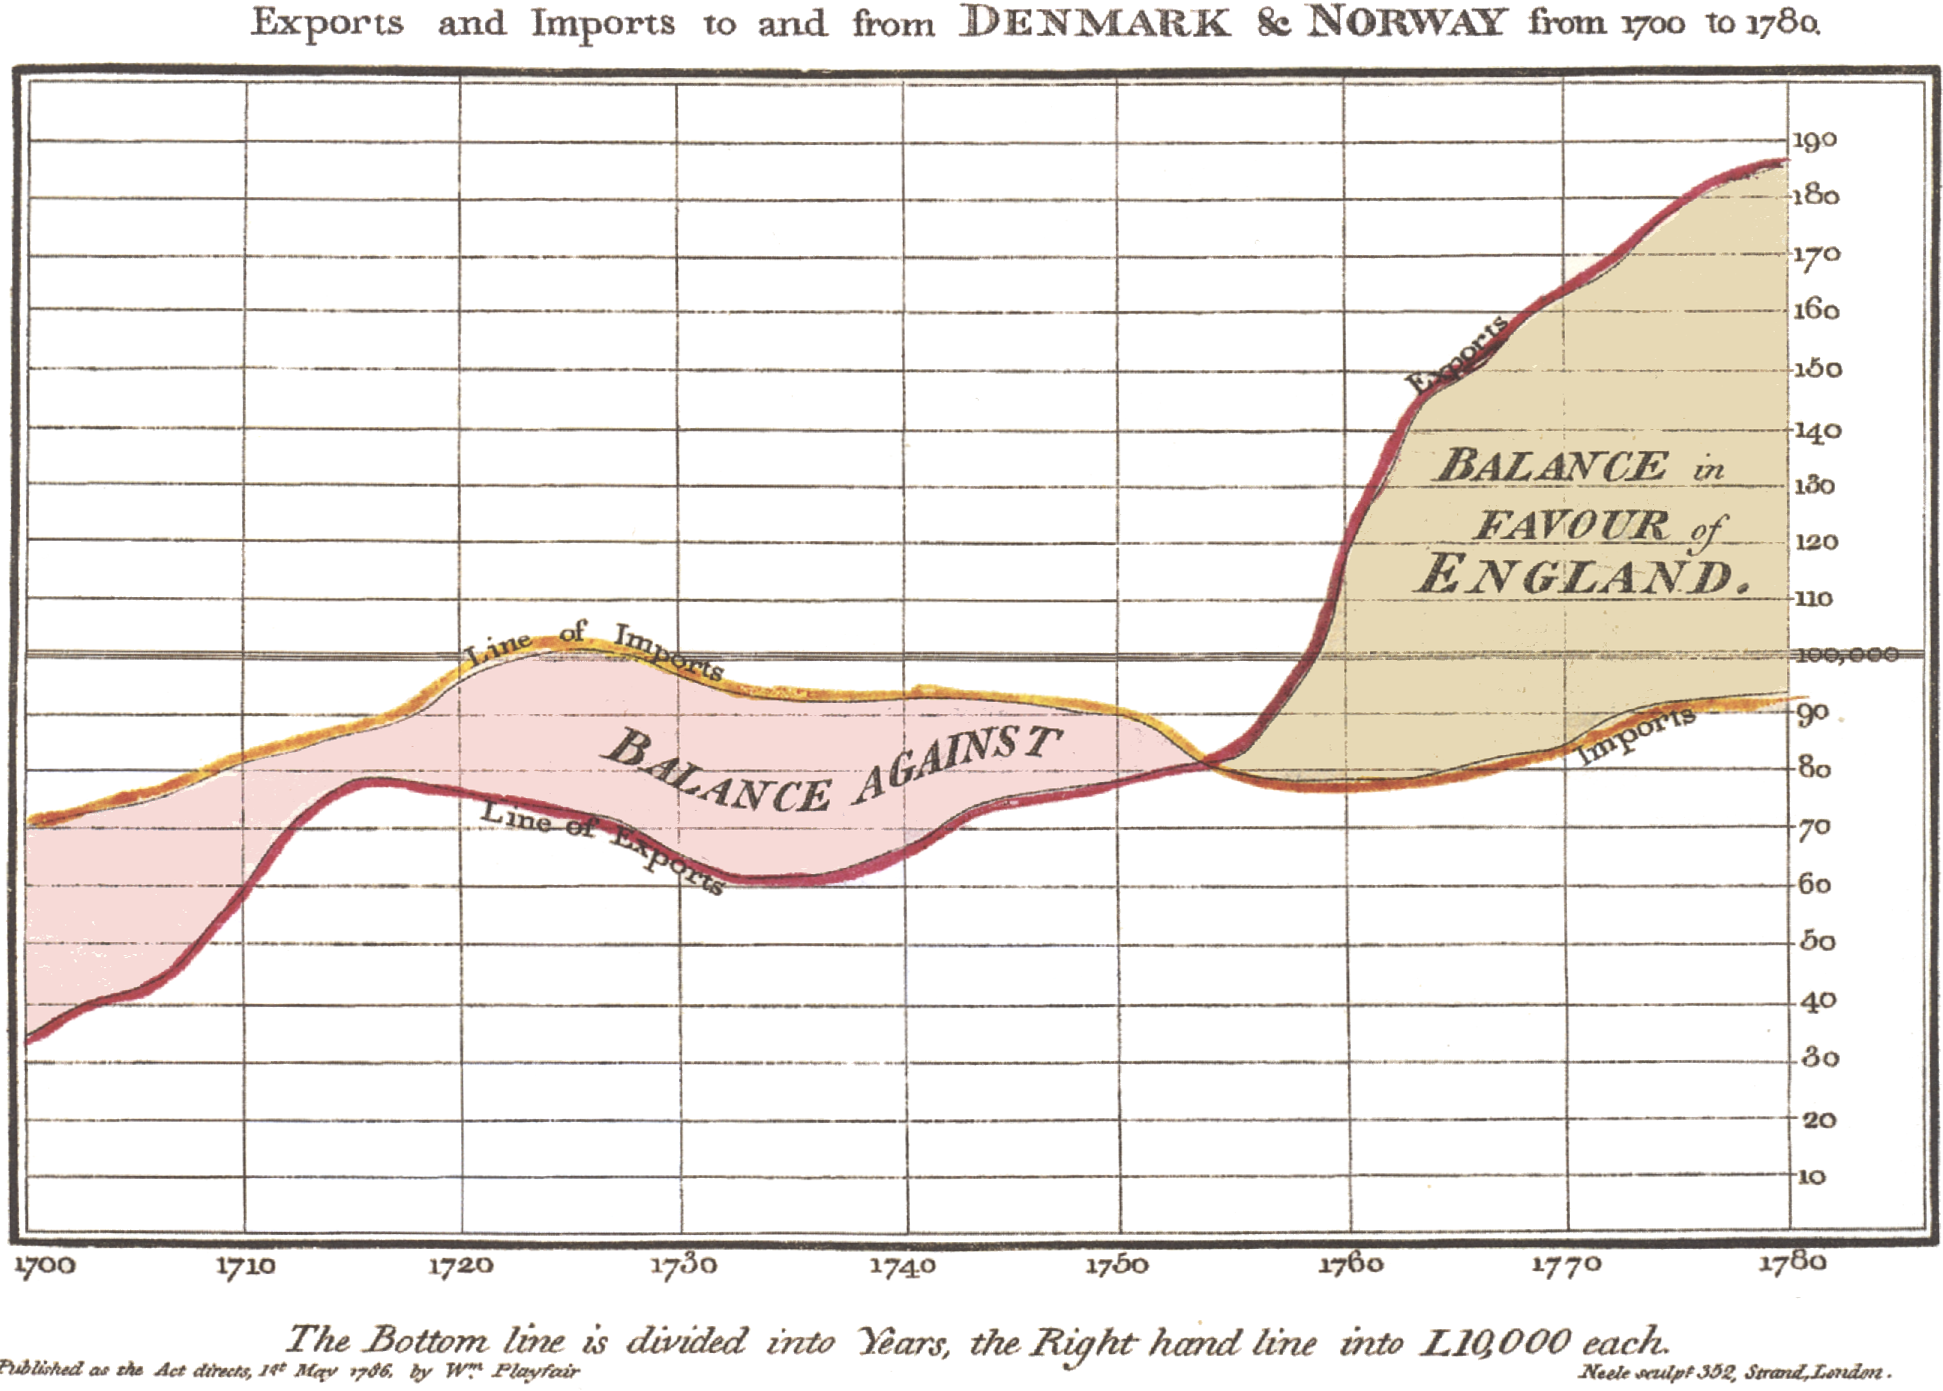
\includegraphics{images/Playfair-TimeSeries} 

}

\caption[William Playfair 的时序线图 ]{\citet{Playfair86} 绘制的线图。 这幅图主要展示了 1700 年至 1780 年间英格兰的进出口时序数据,左边表明了对外贸易对英格兰不利,而随着时间发展,大约 1752 年后,对外贸易逐渐变得有利。图片来源: \url{https://en.wikipedia.org/wiki/William_Playfair}}\label{fig:playfair86}
\end{figure}



\begin{figure}

{\centering \subfloat[\label{fig:playfair01-1}]{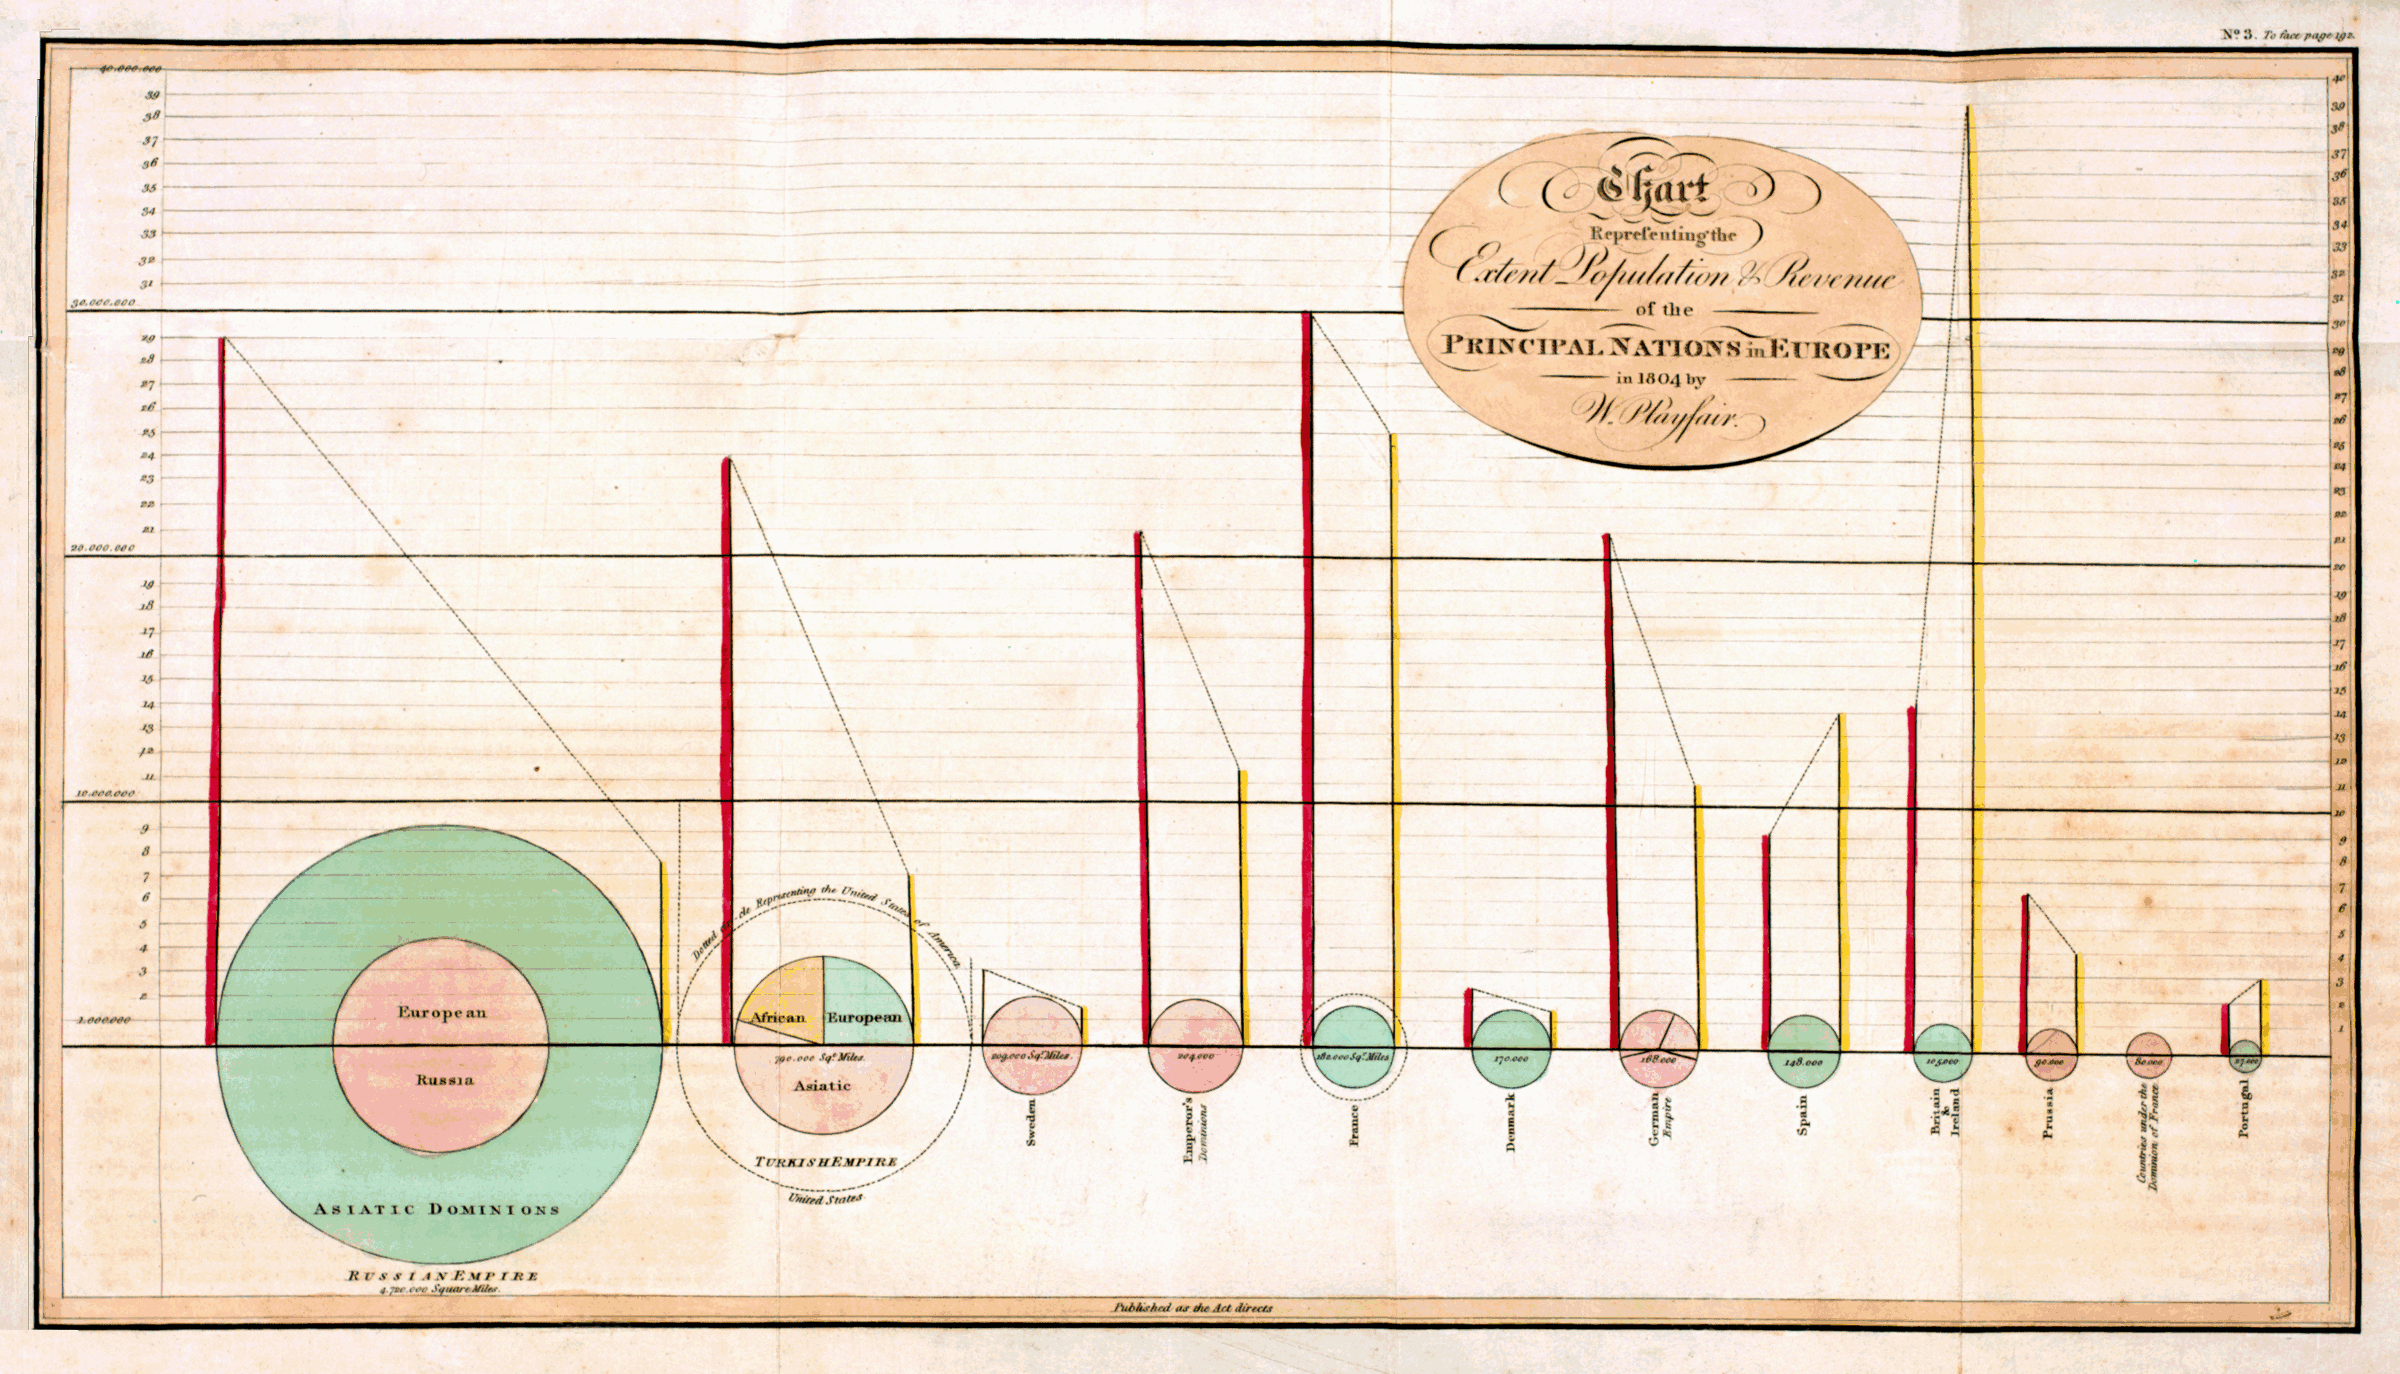
\includegraphics{images/Playfair-pie1} }\newline\subfloat[\label{fig:playfair01-2}]{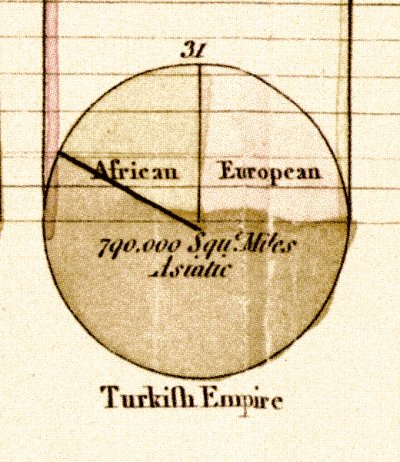
\includegraphics{images/Playfair-pie2} }\newline

}

\caption[William Playfair 的饼图 ]{\citet{Playfair01} 绘制的饼图。这是历史上最早出现的饼图,描述了法国大革命前后一些欧洲国家的统计数据。上方的大图展示了各个国家的领土面积(和圆圈成比例)以及人口(左垂线)、税收(右垂线)、国土在各大洲分布比例等数据,两条垂线连线的斜率可表示税负的轻重(这一点颇有争议,因为斜率与圆的半径有关)。下方的饼图展示了土耳其帝国在三大洲的国土面积分布。图片来源:\url{https://en.wikipedia.org/wiki/William_Playfair},\url{https://www.math.usu.edu/~symanzik/papers/2009_cost/editorial.html}}\label{fig:playfair01}
\end{figure}



\section{霍乱传染之谜}\label{sec:the-mystery-of-cholera-infection}

袭击欧洲大城市最严重的天灾要数 19 世纪的霍乱。由于垃圾没有得到及时清理,清洁水源的缺少,以及下水管道系统的不足,伦敦成为无药可医的流行病滋生的最佳地点。公众一致认为霍乱是由空气传播的,如果呼吸到了``瘴气''或者接触到霍乱患者,就会染上这种病。医生兼自学成才的科学家 John Snow 对这个观点颇为怀疑,他决心通过彻底调查这种致命疾病的根源来证实他的怀疑。

通过和当地居民交谈,他确定了霍乱爆发的源头是位于 Broad 大街的公共水泵。他对这种疾病类型的研究看起来很可信,因此他成功说服了当地政府废弃那个水泵。他所利用的主要证据就是图 \ref{fig:snow-cholera}:死亡发生的地点有明显的地理规律,在这种规律的指引和相关调查证据的支持下,他最终确定了霍乱的源头。后来证实离这口井仅三英尺远的地方有一处污水坑,坑内释放出来的细菌正是霍乱发生的罪魁祸首。

\begin{figure}

{\centering \href{https://en.wikipedia.org/wiki/John_Snow_(physician)}{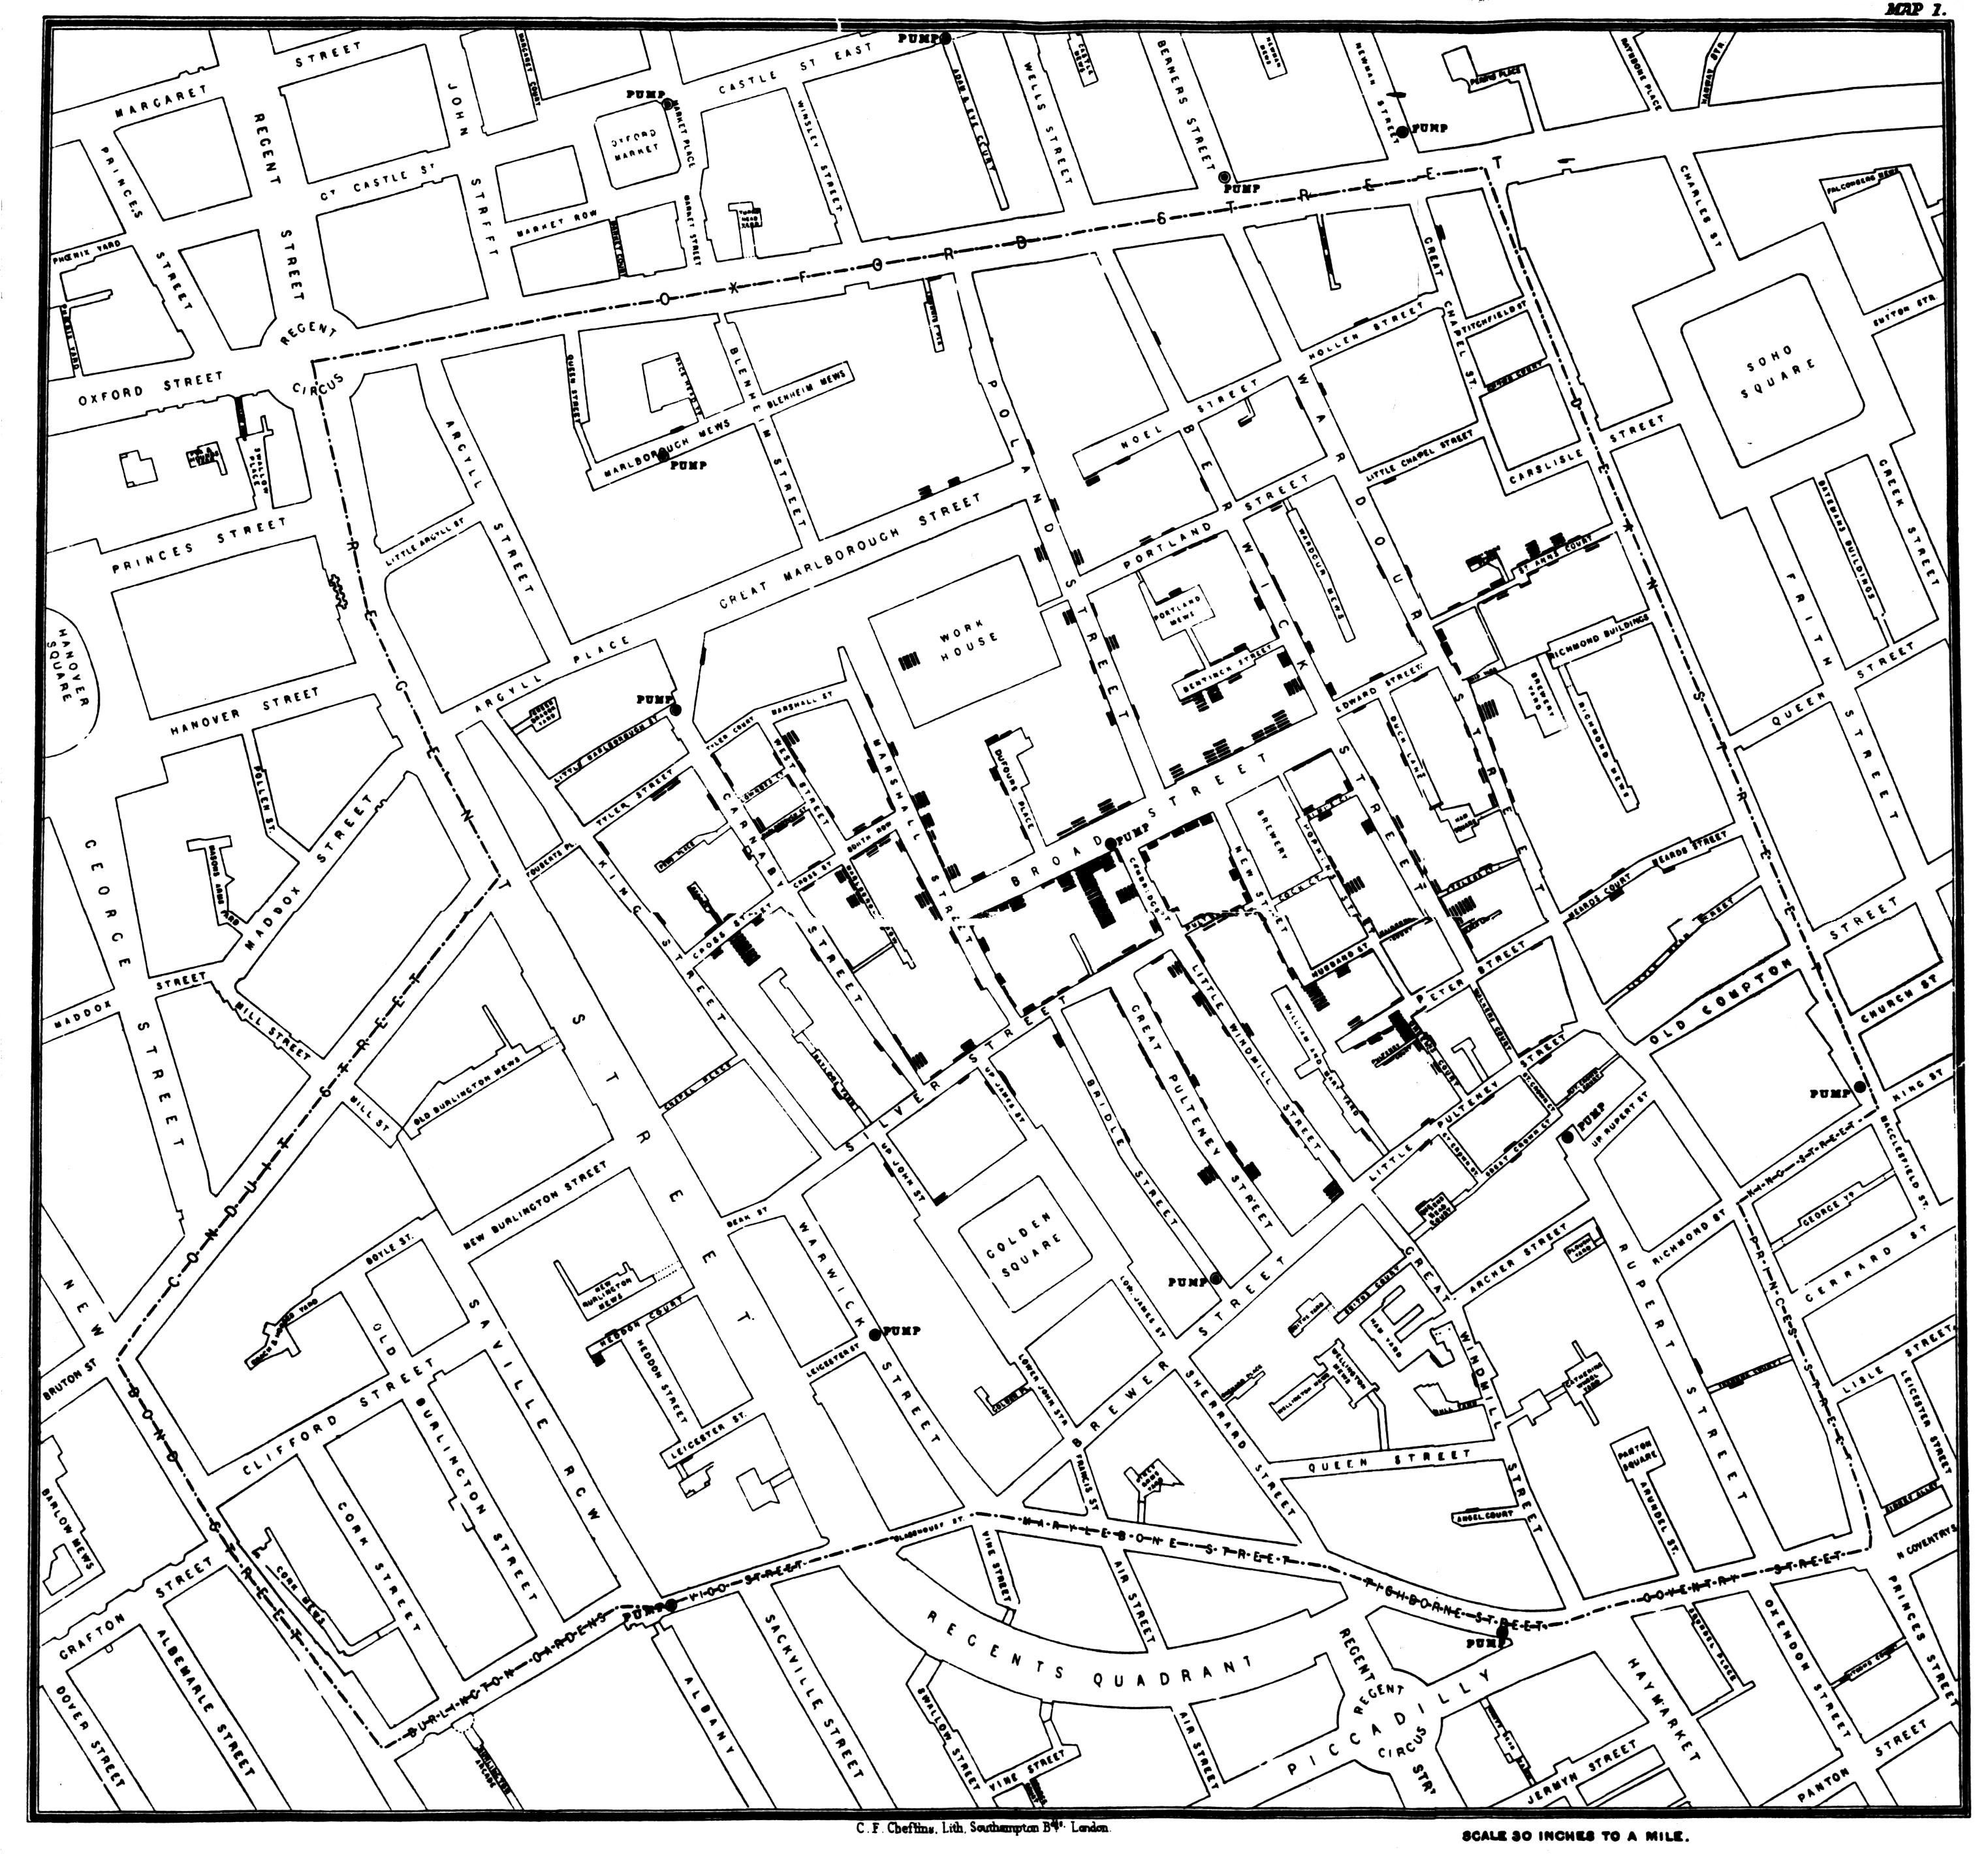
\includegraphics{images/Snow-cholera-map} }

}

\caption[John Snow 的霍乱传染原因探索图]{1854 年英国 Broad 大街大规模爆发霍乱,当时了解微生物理论的人很少,人们不清楚霍乱传播途径,而``瘴气传播理论''是当时的主导理论;John Snow 对这种理论表示了怀疑,于 1849 年发表了关于霍乱传播理论的论文,本图即其主要依据。图中心东西方向的街道即为 Broad 大街,黑点表示死亡的地点,黑点叠加的高度相应表示了该处死亡人数。这幅图形揭示了一个重要现象,就是死亡发生地都在街道中部一处水源(水井)周围,市内其它水源周围极少发现死者。进一步调查他发现这些死者都饮用过这里的井水}\label{fig:snow-cholera}
\end{figure}



\section{提灯女士的玫瑰图}\label{sec:nightingale}

南丁格尔(Florence Nightingale)是我们耳熟能详的``提灯女士'',她不仅是现代护理的鼻祖及现代护理专业的创始人,而且是历史上使用极坐标面积图的先驱。这种图形外形如玫瑰,因此后来也称之为玫瑰图,其主要构思是用``花瓣''的面积表示统计数值的大小。图 \ref{fig:nightingale-mortality} 反映了克里米亚战争(英国等与俄国争夺巴尔干半岛的战争)中英国军队自 1854 年 4 月至 1856 年 3 月的逐月死亡人数 \citep{Nightingale58};其中,右图为 1854 年 4 月至 1855 年 3 月的死亡人数,左图为 1855 年 4 月至 1856 年 3 月的死亡人数。玫瑰图不仅清楚展示了这两年军队死亡人数的变化,而且更重要的是,她将每个月中三种死亡情况也分别用不同颜色标记出来:蓝色表示死于可预防的疾病、红色表示死于战争伤害、黑色表示死于其它原因。这样我们可以清楚知道军队伤亡原因的结构,尤其是``绝大多数士兵死于可预防的疾病''(图中最高的花瓣)。凭借这一条重要信息,她让英国政府意识到,真正影响战争伤亡的并非战争本身,而是由于军队缺乏有效的医疗护理!

\begin{figure}

{\centering \href{<https://en.wikipedia.org/wiki/Florence_Nightingale>}{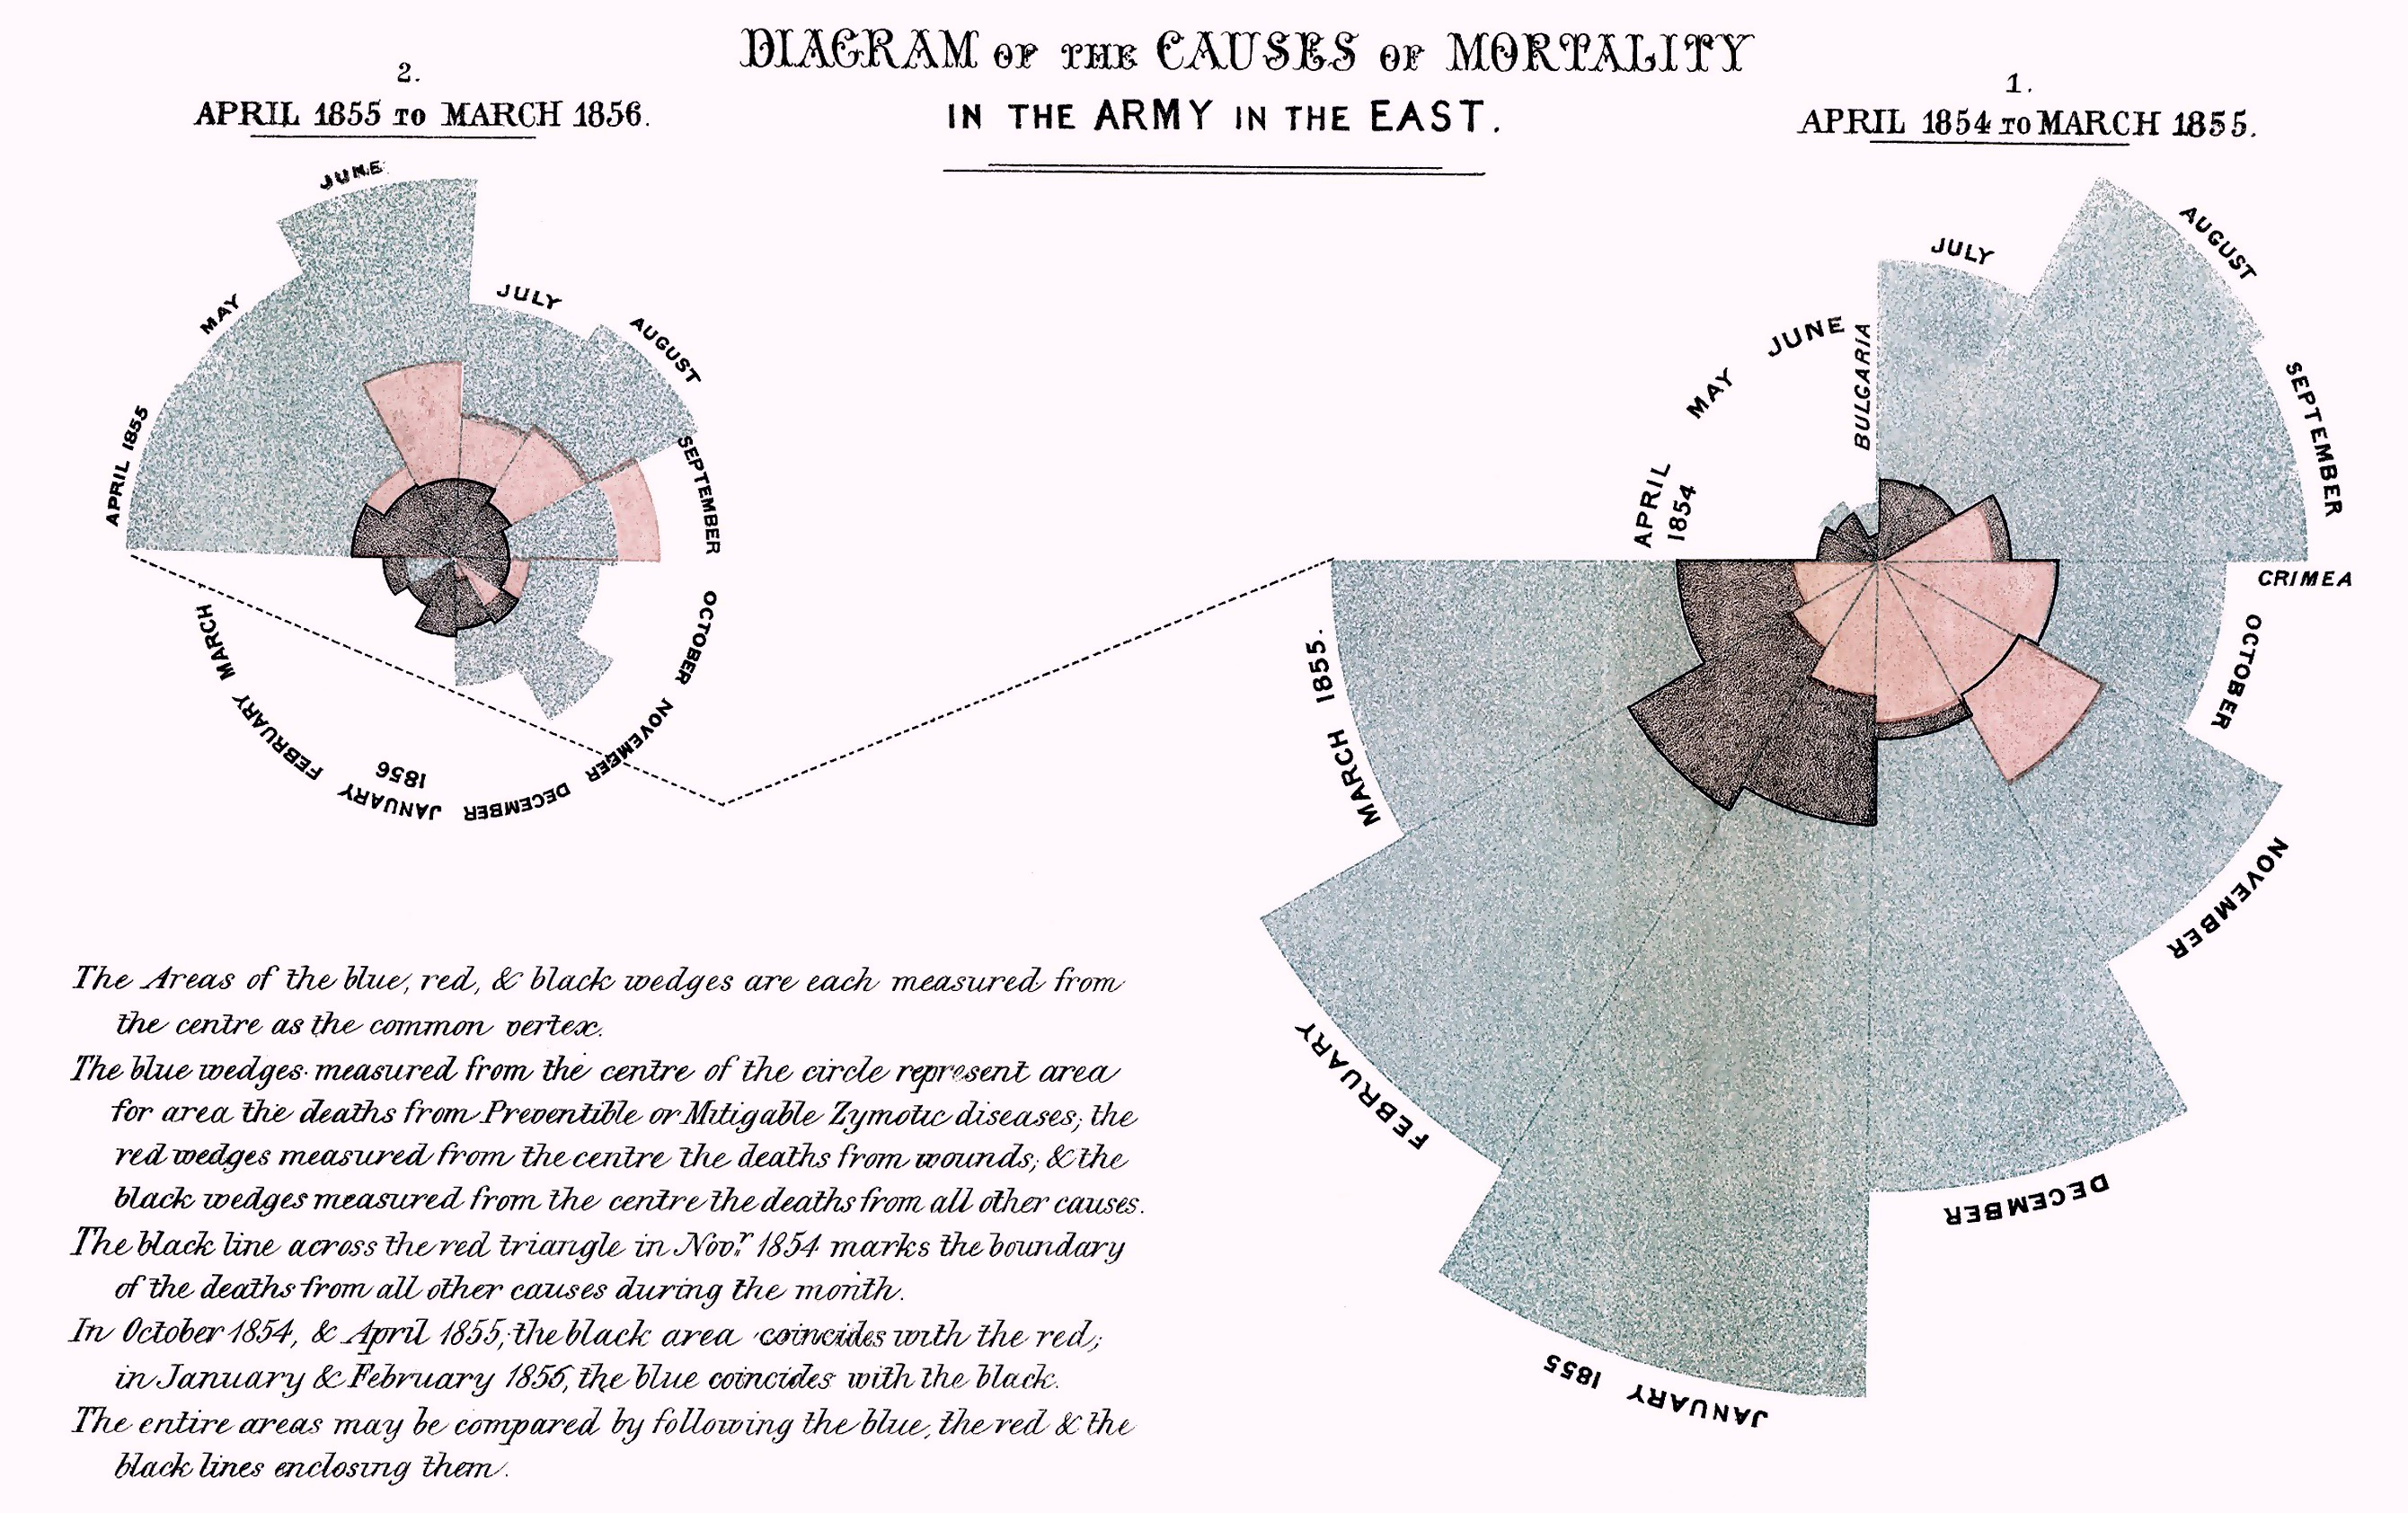
\includegraphics{images/Nightingale-mortality} }

}

\caption[Florence Nightingale 的极坐标面积图]{南丁格尔的极坐标面积图:两幅图分别是 1854 年和 1855 年的军队伤亡人数,一年 12 个月恰好可以将极坐标分为 12 等分,每一瓣代表一个月。图中用颜色标记出了三种死亡原因。南丁格尔的重大贡献在于使得英国政府意识到真正影响战争伤亡的并非战争本身,而是由于军队缺乏有效的医疗护理,导致大量的士兵死于可预防的疾病。1857 年,在她的努力下,英国皇家陆军卫生委员会成立。同年,军医学校成立。}\label{fig:nightingale-mortality}
\end{figure}





\section{拿破仑的俄罗斯远征}\label{sec:charles-joseph-minard}



\begin{figure}

{\centering \href{https://en.wikipedia.org/wiki/Charles_Joseph_Minard}{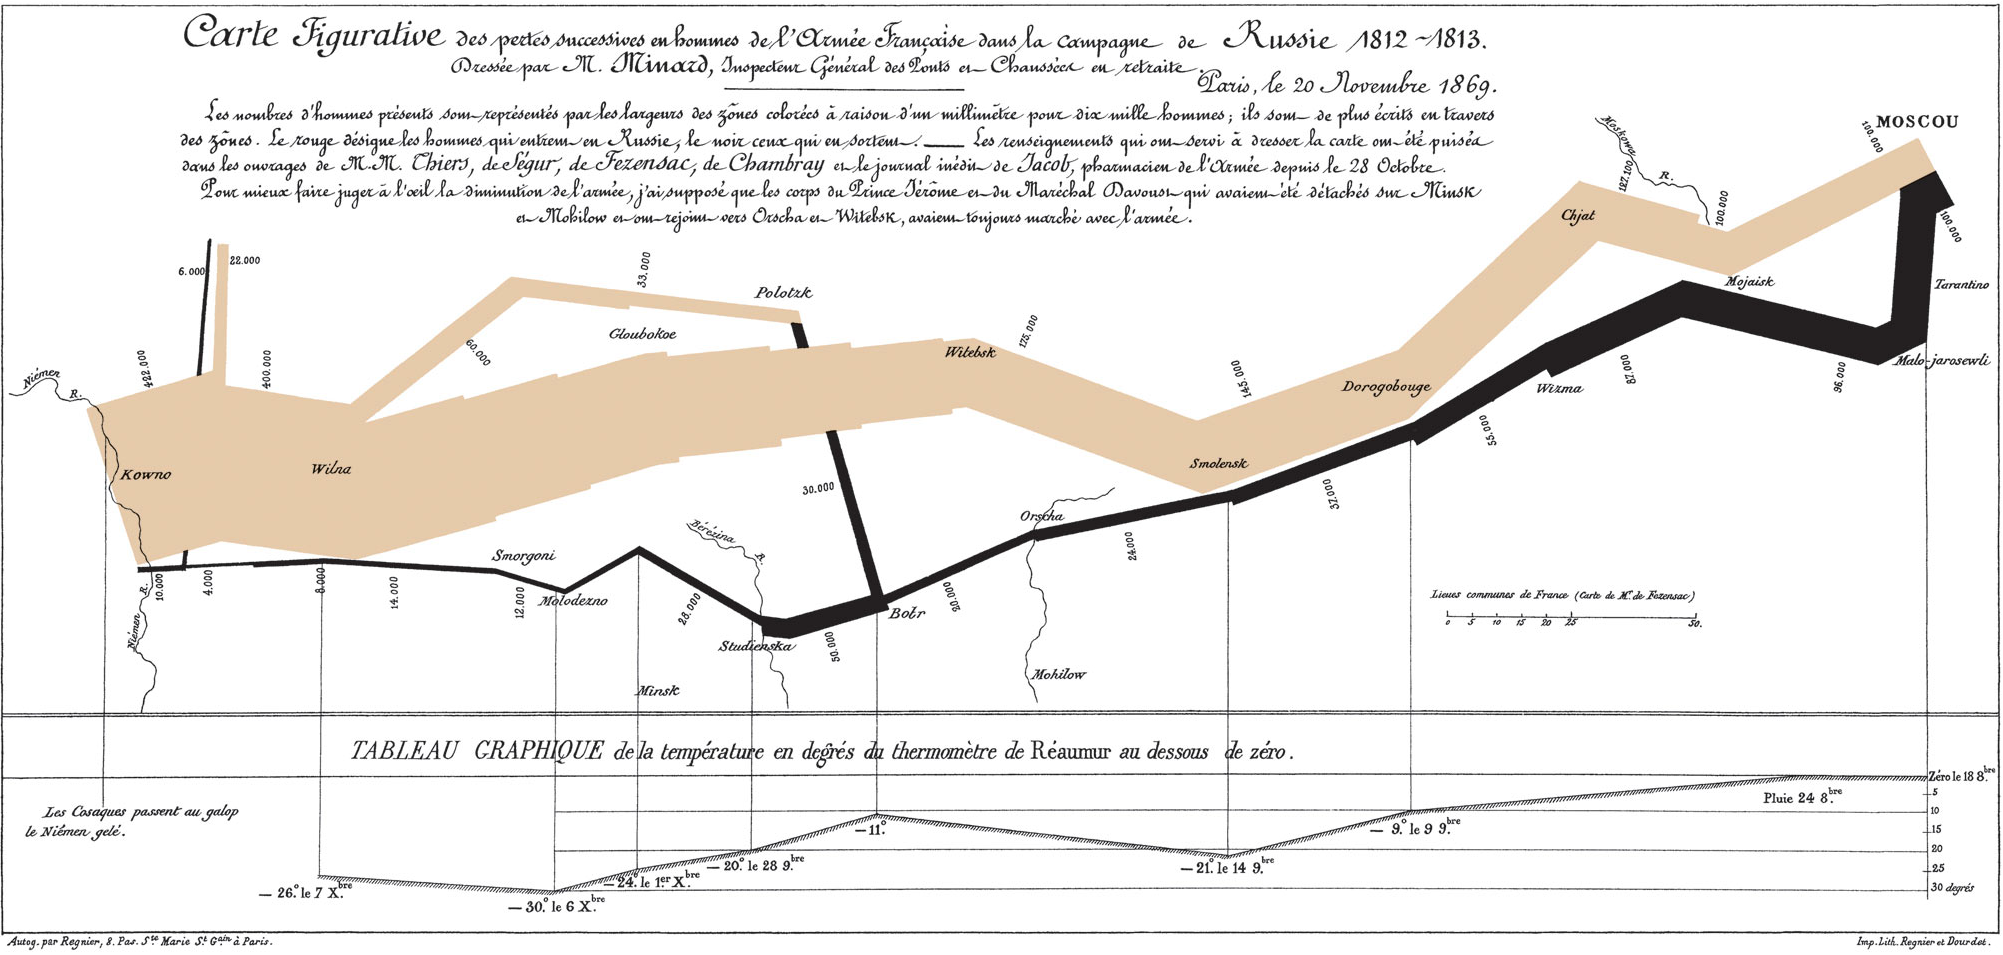
\includegraphics{images/Minard} }

}

\caption[Charles Joseph Minard 的拿破仑远征图 ]{Minard 绘制的地图,展现了 1812 年拿破仑的大军团进军俄国的路线(上半部分)和撤退时的气温变化(下半部分)。这一历史事件中,法军数量的急剧减少以及恶劣的气候条件一览无遗,法国科学家 Étienne-Jules Marey 称``该图所展现出的雄辩对历史学家的笔是一种极大的挑战''}\label{fig:minard}
\end{figure}

1812 年 6 月 24 日,拿破仑率领的 691,501 人的大兵团---同时也是欧洲历史上集结的最大规模的部队---开赴莫斯科。但等他们到达那里,看到的只是一座空城。城里的人都被遣散,所有的供给也被中断。由于没有正式的投降,拿破仑觉得俄国人从他那儿剥夺了一场传统意义上的胜利。

军队不得不撤退。在归程中,因为天气过于恶劣,给军队提供补给几乎是不可能的。马匹因为缺少粮草而变得虚弱,所有的马要么饿死,要么被饥饿的士兵拿去果腹。没有了坐骑,法国骑兵们成了步兵,大炮和马车被迫丢弃,部队没了装甲。饥饿与疾病带来惨重的伤亡,而逃兵数目也直线上升。大军团的小分队在 Vyazma,Krasnoi 和 Polotsk 也被俄国人击溃。法国军队在渡贝尔齐纳河时遭到俄军两面夹击,伤亡惨重,这也是法军在俄国遭遇的最后一场灾难。1812 年 12 月 14 日,大军团被驱逐出俄国领土。在这场远征俄罗斯的战役中,拿破仑的士兵只有大约 22,000 人得以幸存。

这一历史事件被 Charles Joseph Minard 用一张二维平面图形记录了下来,Minard 是一位法国工程师,他以在工程和统计中应用图形而闻名。图 \ref{fig:minard} 就是他的著名作品:在一张二维图形中,他成功地展示了如下信息:

\begin{itemize}
\tightlist
\item
  军队的位置和前进方向,以及一路上军队的分支和汇合情况
\item
  士兵数目的减少(图形顶端最粗的线条表示最初渡河的 422,000 人,他们一路深入到俄国领土,在莫斯科停下来的时候还有 100,000 人左右。从右到左,他们朝西走回头路,渡过 Niemen 河的时候,仅仅剩下 10,000。随着大部队和余部会师(比如在渡贝尔齐纳河之前),图中显示的数字降中也有升)
\item
  撤退时的气温变化(参见图的下半部分,可知当时气候条件极其恶劣)
\end{itemize}

这幅图形在统计图形界内享有至高无上的地位,被 Edward Tufte 称为``有史以来最好的统计图形''(Tufte 是统计图形和信息可视化领域的领军人物,人称``数据达芬奇'')。

\section{小结与开始}\label{sec:begin}

在前面四节中,我们看到了具有历史意义的几幅统计图形,它们融入了前人的智慧与艺术,有些甚至具有重大社会价值。当然我们不能苛求每一幅统计图形都能达到那样的效果,但至少我们了解到了统计图形在揭示特殊现象或规律上的功能,这种功能是数据本身不能替代的。试想,若只是将每一个霍乱死者的数据列在纸上,那么要观察出霍乱发生的规律是何其艰难。

统计图形领域还有大批卓有成就的研究者,为统计图形的发展做出了不少贡献。在上个世纪八九十年代甚至更早,国外已经有比较全面的图示书籍文献资料,如前文提到的``数据达芬奇'' Tufte,他的著作如 \citet{Tufte92} 和 \citet{Tufte01} 在可视化领域有非常深远的影响,他本人于 2010 年被奥巴马政府聘请加入``经济复苏独立咨询小组''(Recovery Independent Advisory Panel),从这一点可见他的成就和威望;但如果说统计图形有一位启蒙思想家的话,那么恐怕非 Tukey 莫属了,\citet{Tukey1977} 提出来的探索性数据分析可以说在当时引领了一个统计学的新方向,在数理统计为主导的统计界注入了一股新活力,探索性数据分析的主要工具就是统计图形,注意 Tukey 本人的数学功底极好,这一点从若干著名统计学家的回忆录中都可以找到证据(统计学刊物 Statistical Science 每一期的最后都有一篇采访,本人在这些采访中时常见到 Tukey 被提及),但从他的一些论文著作中我们可以看到他非常重视数据分析,\citet{Tukey62} 就是一篇很好的例证(他认为数学不是一门科学,而数据分析则是);Tukey 常常体现在一些细节之处展现他的观察力,令人不得不感到佩服,例如 \citet{Wainer81} 中提到了一件事:过去人们常用斜线计数,\(\text{/}\) 表示 1,\(\text{//}\) 表示 2,\ldots\ldots,达到 4 条线(\(\text{////}\))之后紧接着用 \(\bcancel{\text{////}}\) 表示 5,但 Tukey 认为这样很容易出错,比如要是在 3 条线之后不小心早划了表示 5 的斜线 \(\bcancel{\text{///}}\),或者在 5 条线之后才画那条反方向的斜线 \(\bcancel{\text{/////}}\),都将造成难以修复的错误,因此他提出了一种新的计数方法:先用正方形的四个顶点分别表示 1、2、3、4,到 4 点的时候就开始连边线,每连一条线就表示数字增加 1,这样 4 条边都连好之后就可以表示到 8 了,最后分别连对角线表示 9 和 10,即 \(\boxtimes\) 表示 10,用这种计数法则不必担心画错线,因为不管连哪条线都是表示 1,其实细心的中文读者马上能联想到我们的``正''字计数法,这个计数法比 Tukey 的方法更具有稳健性;统计图形一直以来都因为缺乏像数学那样的理论而受人诟病,关于这一点,\citet{Wilkinson05} 则给出了一个很好的框架,它也是 R 包 \textbf{ggplot2} 的理论基础;贝尔实验室的的 Cleveland 在图形认知方面做了不少工作,告诉我们应该怎样合理构建图形以及解读图形,如 \citet{Cleveland85} 和 \citet{Cleveland93} 等,其中值得一提的是他可能是最早研究统计图形对读者心理感知的影响的统计学家之一,但不幸的是,这项工作似乎并没有引起人们的广泛重视(饼图直至今日仍然泛滥便是一个最好的例证),另外他提出了 S 语言中的 Trellis 图形,这对统计图形软件的发展来说也是具有划时代意义的贡献,后来 R 语言中的 \textbf{lattice} 包正是继承了 Trellis 图形的概念,近些年来也非常有影响力。关于统计图形的历史总结,\citet{Friendly01} 是一份非常详尽的资料,该文档整理、记载了自 17 世纪以前至今数百年历史中较有影响力的统计图形。

近代统计图形以 \citet{Tukey1977} 的探索性数据分析为里程碑式的起点,诞生了大批具有数理统计意义和计算机应用的图形著作和图形种类,如我们熟知的箱线图 \citep{McGill78},LOWESS 曲线 \citep{Cleveland79},直方图和密度曲线 \citep{Scott92},基于 S 语言的著作 \citep{Chambers83} 以及注重表达信息的著作(如前文介绍的 Tufte)等;现代统计图形的发展则更偏重计算机工具的开发以及高维图形和动态图形的展示,其中 S 语言 \citep{Becker88} 为现代统计图形的发展奠定了重要的基础,随后 R 语言 \citep{Ihaka96, base} 的兴起,更是带来了数不胜数的统计图形方法,比较有代表性的如 R 语言的基础包 \textbf{graphics} 包和 \textbf{grid} 包 \citep{Murrell05}、基于 Trellis 图形 \citep{Cleveland93} 思想的 lattice 图形 \citep{Sarkar08}、基于统计图形理论著作 \citet{Wilkinson05} 的 ggplot2 图形 \citep{ggplot2}、基于动态图形 GGobi 软件 \citep{Cook07} 的高维数据交互图形实现 \textbf{rggobi} 包 \citep{rggobi}、基于 OpenGL 的三维动态图形系统 \textbf{rgl} 包 \citep{rgl} 和分类数据图示的 \textbf{vcd} 包 \citep{vcd} 等,此外,还有一批新的高维图形思想被提出,如打破笛卡尔坐标系常规的平行坐标图 \citep{Inselberg07},并出现了一些 R 语言之外的独立交互图形软件如用于分析缺失值的 MANET 软件 \citep{Unwin96} 和交互式图形分析软件 Mondrian \citep{Theus02} 等,这些动态图形和交互图形的综述可参考 \citet{Jurgen04}。

如今统计图形的使用看似已经比较普遍,饼图、条形图都已不是什么新鲜内容,人人都能做,但是,一方面统计图形的价值并没有被很好地体现出来,另一方面人们对统计图形的了解也被统计软件所限,而不能随心创造图形。我们来看这样一组事实 \citep{Xie08}:

\begin{quote}
以期刊《统计研究》在 2006 年 12 月 \textasciitilde{} 2007 年 11 月期间共 12 个月的所有论文作为统计对象,剔除部分非学术研究型论文之后,挑选论文总数为 168 篇,其中使用表格的论文篇数为 136 篇(81.43\%),表格总数为 528 个,而使用图形的论文仅有 63 篇(37.72\%),若将仅仅使用示意图(非统计图形)、条形图和折线图的论文排除在外,使用其它图形的论文仅剩下 9 篇。
\end{quote}

这可算国内统计图形应用现状的一个缩影。为了改变这种局面、发掘出统计图形在数据分析中应有的潜力,我们特别撰写这本书,供广大统计研究者参考。我们的目的并非仅限于如何作出漂亮的统计图形,而是在作图的同时,强调图背后更重要的工作,那就是``数据分析与统计图形的有机结合''。传统的统计分析大约可以分为三类:

\begin{itemize}
\tightlist
\item
  描述性统计分析:Descriptive Statistical Analysis
\item
  推断性统计分析:Inferential Statistical Analysis
\item
  探索性统计分析:Exploratory Statistical Analysis
\end{itemize}

前两类统计分析往往都是从既定的统计模型、方法的角度入手,而探索统计分析则主要借助图形对数据进行探索性分析,这对于数据分析的手段是一种重要的拓展(姑且称之为``图形统计分析'');然而要使用这种手段,则必须清楚了解如何制图以及现有图形有哪些种类,这样才能真正开发出统计图形的价值。

其实,``图形统计分析''也不是一个新概念,平常的统计图示已经或多或少用到了这样的思想,只是我们往往更倾向于数理意义上的统计模型分析,而不会把图形统计分析作为主要分析手段。当然,由于图形的表达限制以及统计图形的普及程度,也使得它不可能替代模型分析,但无论如何,我们对统计图形在统计分析中的地位应该加深认识,不仅是因为这是一个信息爆炸的时代、大量的信息让我们无法在短时间内获取核心信息,更重要的是,目前在国内仍有大量的统计图形未被开发介绍出来,图形种类过于单一,表达信息的效果大打折扣。

本书介绍统计图形的方式主要是从两方面入手,第一,阐明各种统计图形所用到的统计量;第二,与实例结合,解释图形中表现的统计量的实际含义。在本书的附录 \ref{cha:tricks} 中,我们也会介绍一些有用的细节和作图技巧,用以辅助完善统计图形。

总的说来,要把图形提到``统计分析''的高度,就一定要搞清楚统计图形的来龙去脉,包括原始数据的来源和类型、统计量的计算、图形的构造与组合机制等,这与统计模型实际上没有本质的区别:若不清楚模型的假设前提、计算原理以及相应的结果解释,同样也不能随便使用模型分析。除了图形本身之外,用好图形分析还需要一定的洞察力,最简单的莫过于观察数据的分布状况、离群点、线性/非线性关系等表面观察,而更重要也是最本质的莫过于洞察到种种规律或异常现象背后的深刻原因,至此,我们才达到了分析的目的。

\section{思考与练习}\label{ux601dux8003ux4e0eux7ec3ux4e60}

\begin{enumerate}
\def\labelenumi{\arabic{enumi}.}
\item
  图 \ref{fig:playfair86} 的主旨是用来刻画贸易顺差或逆差,因此把出口额和进口额画在同一幅图上似乎是自然而然的选择,但是我们真正关心的是两条曲线之差。你认为 Playfair 的这幅图是否存在不足、以及应该怎样改进?
\item
  某种程度上,Tukey 引导了``用数据说话''的潮流,这样的做法有什么潜在危险?换句话说,当我们浏览一幅图形的时候,我们首先要考虑的是数据的来源,如果我们忽略数据的来源而直接去考虑基于图形的发现,所谓的``数据说的话''是什么话?
\item
  统计图形和统计模型的最大区别在哪里?提示:并非高下之分,而是二者各自的假设是什么。更具体地,我们知道数理统计中的假设检验通常有零假设和备择假设,统计图形更像在研究哪一个假设,而统计模型又通常研究哪一个?
\end{enumerate}

\chapter{工具}\label{cha:tools}

\begin{quote}
``好了,好了,我的好伙计,就这么办吧。我们在这房子里共同生活了好几年,如果再蹲在同一座牢房里就更有意思了。华生,我跟你说实话。我一直有个想法:我要是当罪犯,一定是超一流的。这是我在这方面难得的一次机会。看这儿!''他从抽屉里拿出一个整洁的皮制小袋,打开来亮出里面几件闪亮的工具。``这是最新最好的盗窃工具,镀镍的撬棒,镶着金刚石的玻璃刀,万能钥匙,以及对付现代文明所需要的各种新玩意儿。我这儿还有在黑暗中使用的灯。一切都准备好了。你有走路不出声的鞋吗?''

\hspace*{\fill} --- 柯南·道尔《查尔斯·密尔沃顿》
\end{quote}

那么我们面对这么多工具应该如何选择呢?我们认为主要的准则有三点:一是统计计算功能齐全,二是统计元素易于控制,三是图形类型丰富多样。

\section{选择作图工具}\label{ux9009ux62e9ux4f5cux56feux5de5ux5177}

在人们通常的观念中,图形往往代表着简单,然而直观与简单是两个不同的概念,图形的首要作用的确是直观展示信息,然而这里的信息未必是简单的。一幅优秀的统计图形背后也许隐藏着重要的统计量,而统计量是统计图形的最关键构成因素。

我们通常见到的所谓统计图形也许只是 Microsoft Office Excel 的产物,事实上,Excel 的图形总体看来只有三种,第一种是表现绝对数值大小,如条形图、柱形图、折线图等,第二种是表现比例,如饼图,第三种则是表示二维平面上的变量关系,如 X-Y 散点图;从更广泛的意义上来说,Excel 展示的几乎都是原始数据,基于数据的统计推断的意味比较淡薄。而统计学的核心研究对象是什么?答案应该是分布(Distribution),注意分布不仅包含一元变量的分布,而且更重要的是多元变量的分布,诸如''均值 ``、''方差''、``相关''和''概率''等概念都可以归为分布的范畴。无论 Excel 的图形如何搭配色彩、怎样变得立体化,都跳不出上面三种类型的限制,而且不能全面妥善表达统计学的要义。可能正是因为这样的原因,统计图形界内的一位大家 Leland Wilkinson 才说给统计刊物投稿时永远不要用 Excel 作图。本书所要介绍的 R 语言能表达的统计量种类极其丰富,甚至可以毫不夸张地说,任何理论上可以计算出来的统计量都能在 R 中很方便地以图形的方式表达出来。

除了统计量之外,我们也应对图形本身的组成元素给予足够的重视,这些元素包括点、线(直线、曲线、线段和箭头等)、多边形、文本、图例、颜色等,往往这部分工作都由常见的统计软件替我们做了---我们不必自己设计点、线等基本元素,但同时也就意味着我们几乎无法灵活运用这些元素(比如在图中添加点、线、文本标注等)。表面上看似计算机软件给我们省了不少麻烦,实际上,这种限制的弊端要大于那一点微不足道的好处。我们在实际工作中遇到不少这样的例子,比如往散点图中添加若干条不同的回归直线(根据某自变量不同分类的回归、或者是不同分位数的分位回归 \citep{quantreg} 直线等)、在图中添加箭头或者文本标注甚至添加包含希腊字母、微积分符号、上下标的数学公式,等等,不一而足,对于这些简单问题,用传统的(商业)统计软件恐怕太难解决,原因就在于,它们让计算机替代了太多本可以由用户完成的工作。当然,总体来说,自动化是好事,但如果为了自动化而大幅度牺牲可定制性,则可能得不偿失了。

相比之下,R 语言汇集统计计算与统计图示两种功能于一身,灵活的面向对象(Object-Oriented,OO)编程方式让我们可以很方便地控制图形输出,从而制作出既精美又专业的统计图形。我们说图形并不意味着简单,指的是统计图形的构造可以很细致入微(包括统计量的选定和图形元素的设计),而不是指 R 作图的过程或程序很复杂。同样,如果我们总是需要在图形细节上耗费大量的精力,那么 R 也将不是一个好工具。在后面第 \ref{cha:elements} 、\ref{cha:gallery} 章和附录 \ref{cha:tricks} 中,我们会介绍若干作图的细节问题,读者需要斟酌美观与效率之间的平衡,避免陷入细节泥潭;实际上 ggplot2 是一个可以大幅减少细节设置的图形系统,我们将会在第 \ref{sec:ggplot2} 小节中详细介绍。

要想真正精通统计图形,则应首先要练好基本功(例如对图形基础元素或构造作深入的了解),然后在此基础上通过各种抽象、提炼和认识最终上升到理性认识的境界(自如地表达统计量)。

\section{R 语言简介}\label{sec:R-intro}

R\citep{base} 是一款优秀的统计软件,同时也是一门统计计算与作图的语言,它最初由奥克兰大学统计学系的 Ross Ihaka 和 Robert Gentleman 编写 \citep{Ihaka96};自 1997 年起 R 开始由一个核心团队(R Core Team)开发,这个团队的成员大部分来自大学机构(统计及相关院系),
包括牛津大学、华盛顿大学、威斯康星大学、爱荷华大学、奥克兰大学等,除了这些作者之外,R 还拥有一大批贡献者(来自哈佛大学、加州大学洛杉矶分校、麻省理工大学等),他们为 R 编写代码、修正程序缺陷和撰写文档。迄今为止,R 中的程序包(Package)已经是数以千计,各种统计前沿理论方法的相应计算机程序都会在短时间内以软件包的形式得以实现,这种速度是其它统计软件无法比拟的。除此之外,R 还有一个重要的特点,那就是它是自由、开源的!由于 R 背后的强大技术支持力量和它在统计理论及应用上的优势,加上目前国内对 R 的了解相对较少,我们期望能够通过本书引进并推动它在国内的广泛使用。

R 的功能概括起来可以分为两方面,一是统计计算(Statistical Computation),二是统计图示(Graphics);一般而言,图形往往比较直观而且相对简易,因此本书从 R 图形入手,以期给初学者提供一份好的 R 作图入门学习资料。

安装好 R 之后,Windows 用户可以从程序快捷方式直接启动 R,Linux 用户则可从终端敲入命令 \texttt{R} 启动;在启动 R 时,屏幕上会显示类似如下信息,告诉我们 R 是由很多贡献者一起协作编写的自由软件,用户可以在一定许可和条件(GPL)下重新发布它:

\begin{Shaded}
\begin{Highlighting}[]
\FunctionTok{cat}\NormalTok{(}\FunctionTok{head}\NormalTok{(}\FunctionTok{system}\NormalTok{(}\StringTok{"R {-}e NULL"}\NormalTok{, }\ConstantTok{TRUE}\NormalTok{)[}\SpecialCharTok{{-}}\DecValTok{1}\NormalTok{], }\DecValTok{16}\NormalTok{), }\AttributeTok{sep =} \StringTok{"}\SpecialCharTok{\textbackslash{}n}\StringTok{"}\NormalTok{)}
\end{Highlighting}
\end{Shaded}

\begin{verbatim}
## R version 4.4.0 (2024-04-24) -- "Puppy Cup"
## Copyright (C) 2024 The R Foundation for Statistical Computing
## Platform: aarch64-apple-darwin20
## 
## R is free software and comes with ABSOLUTELY NO WARRANTY.
## You are welcome to redistribute it under certain conditions.
## Type 'license()' or 'licence()' for distribution details.
## 
##   Natural language support but running in an English locale
## 
## R is a collaborative project with many contributors.
## Type 'contributors()' for more information and
## 'citation()' on how to cite R or R packages in publications.
## 
## Type 'demo()' for some demos, 'help()' for on-line help, or
## 'help.start()' for an HTML browser interface to help.
\end{verbatim}

从技术上来讲,R 是一套用于统计计算和图示的综合系统,它由一个语言系统(R 语言)和运行环境构成,后者包括图形、调试器(Debugger)、对某些系统函数的调用和运行脚本文件的能力。R 的设计原型是基于两种已有的语言:S 语言 \citep{Becker88} 以及 Sussman 的 Scheme,因此它在外观上很像 S,而背后的执行方式和语义是来自 Scheme。

R 的核心是一种解释性计算机语言,大部分用户可见的函数都是用 R 语言编写的,而用户也可以调用 C、C++ 或者 FORTRAN 程序以提高运算效率。正式发行的 R 版本中默认包括了 \textbf{base}(R 基础包)、\textbf{stats}(统计函数包)、\textbf{graphics}(图形包)、\textbf{grDevices}(图形设备包)、\textbf{datasets}(数据集包)等基础程序包,其中包含了大量的统计模型函数,如:线性模型/广义线性模型、非线性回归模型、时间序列分析、经典的参数/非参数检验、聚类和光滑方法等,还有大批灵活的作图程序。此外,附加程序包(add-on
packages)中也提供了各式各样的程序用于特殊的统计学方法,但这些附加包都必须先安装到 R 的系统中才能够使用 \citep{Hornik-FAQ}。

本书不会过多涉及到附加包,所介绍图形主要基于 R 自身的 \textbf{graphics} 包,当然也不可避免会使用 \textbf{base} 和 \textbf{grDevices} 等基础包中的函数,这些基础包一般不用特别加载,R 在启动的时候会自动加载进来;在第 \ref{cha:gallery} 章中会使用一些附加包介绍特殊的统计数据和统计方法、模型涉及到的图形,例如分类数据(Categorical Data)会提到 \textbf{vcd} 包,生存分析会用到 \textbf{survival} 包。当我们需要调用附加包时,可以使用 \texttt{library()} 函数,例如加载 \textbf{MSG} 包:

\begin{Shaded}
\begin{Highlighting}[]
\FunctionTok{search}\NormalTok{()}
\end{Highlighting}
\end{Shaded}

\begin{verbatim}
##  [1] ".GlobalEnv"        "package:formatR"   "package:stats"    
##  [4] "package:graphics"  "package:grDevices" "package:utils"    
##  [7] "package:datasets"  "package:methods"   "Autoloads"        
## [10] "package:base"
\end{verbatim}

R 的官方网站 \url{https://www.R-project.org} 中对 R 有详细介绍,我们也可以从它在世界各地的镜像(CRAN:\url{https://CRAN.R-project.org},全称 Comprehensive R Archive Network)下载 R 的安装程序和附加包,通常我们可以在 R 中用函数 \texttt{install.packages()} 安装附加包,Windows 用户也可以从菜单中点击安装:Packages \(\Rightarrow\) Install Package(s)),注意,附加包都是从镜像上下载的,因此安装时要保证网络连接正常;当然我们也可以先将程序包下载到本地计算机上然后安装。

可能令读者感到不便的一点是,R 不像别的统计软件那样有图形用户界面(GUI,即 Graphical User Interface,后面附录 \ref{cha:GUI} 会详细介绍),因此它不会显得很傻瓜,它的界面常常是命令行界面(CLI,即 Command Line Interface),即:输入一些代码,R 就会输出相应的运算结果或其它输出结果。因此,在正式使用 R 之前,我们有必要大致了解一下 R 的运作方式。

计算机科学家 Nikiklaus Wirth 曾经提出,程序语言的经典构成是``数据结构+算法'':数据结构是程序要处理的对象,算法则是程序的灵魂。R 也不例外,它有自己独特的数据结构,这些数据结构尤其适应统计分析的需要,它们包括:向量(vector)、矩阵(matrix)、数据框(data frame)、列表(list)、数组(array)、因子(factor)和时间序列(ts)等。当然,数值、文本和逻辑数据都可以在 R 中灵活使用,附录 \ref{sec:object} 中给出了一些简单的数据操作例子,请读者通过阅读该章熟悉 R 的数据对象;至于算法,我们暂时可以不去过多了解,因为 R 中已经包含了大量设计好的函数,对于一般的用户来讲都不必自行设计算法,除非有特殊或者自定义的算法,那么也可以根据 R 的语法规则编写程序代码。

对 R 的运作方式粗略了解之后,我们再回头看看 GUI。一个软件的菜单、按钮、对话框等 GUI 组件不可能无限增多,否则软件会变得无比庞大臃肿,而繁杂的操作顺序的难度将很可能会超过使用程序命令行的难度,而且非开源的 GUI 隐藏了计算原理,除了程序的原始编写者,无人知道输出结果究竟是以怎样的方式计算出来。随着统计学的发展,各种新方法、模型必将不断涌现,我们现在不妨试想未来的统计软件用户界面将会变成什么样子。看看 R 的发展,可以体会到这种思路:菜单不可能无限增加,但是程序、函数都是可以无限增加的---道理很简单,因为它们不受计算机屏幕的限制。迄今为止,R 的仓库(repository)中附加包的数量已经超过 14800 个,这还只是 CRAN 上的仓库,不算另外两个站点 \href{https://www.bioconductor.org/}{Bioconductor}、 \href{https://r-forge.r-project.org/}{R-Forge} 和 \href{http://www.omegahat.net/}{Omegahat},以及 \href{https://github.com}{Github} 上处于开发状态的。在这样的大仓库中,我们可以找到最前沿的统计理论方法的实现,所需做的仅仅就是下载一个通常在几十 K 到几百 K 的一个附加包。值得注意的是,R 的主安装程序大小约为 70 M。相比之下,SPSS 的安装程序已达六七百 M,而 SAS 的基本安装程序也有数百 M,从程序大小角度便可知 R 语言的精炼。

关于 R 更深入的介绍,请参考官方发行的若干手册和网站上的大量学习材料,如官方的 7 本手册(均可从 R 的安装目录或者网站 \url{https://cran.r-project.org/manuals.html} 上找到):

\begin{itemize}
\tightlist
\item
  An Introduction to R (R-intro)
\item
  R Data Import/Export (R-data)
\item
  R Installation and Administration (R-admin)
\item
  Writing R Extensions (R-exts)
\item
  R Internals (R-ints)
\item
  The R Language Definition (R-lang)
\end{itemize}

其中 R-intro 手册附录 A 中给了一个很好的代码入门演示,推荐读者通过这个演示初步熟悉 R 语言;其它手册都比较偏重 R 的底层介绍,不适合对计算机程序没有深入了解的初学者阅读;另外还有 Emmanuel Paradis 编写的《R for Beginners》也是较好的入门教材(已由本书作者及其他几位合作者翻译为中文,可从统计之都 \url{https://cosx.org} 获得);丁国徽也已将几本官方手册翻译为中文,R-intro 的中文翻译文档可以在官方网站上下载。鉴于目前 R 的中文资料并不多,我们也推荐 R 的初学者和爱好者通过访问统计之都网站及其 R 语言版块 \url{https://d.cosx.org/t/r} 共同学习、讨论和研究。

最后需要特别指出的是,R 拥有一套完善而便利的帮助系统,这对于初学者也是很好的资源。若已知函数名称,我们可以简单用问号 \texttt{?} 来获取该函数的帮助,比如查询计算均值的函数帮助,只需要在命令行中敲入 \texttt{?mean},则会弹出一个窗口显示该函数的详细说明。大多数情况下 \texttt{?} 等价于 \texttt{help()} 函数;但有少数特殊的函数在查询其帮助时需要在函数名上加引号,比如 \texttt{?+} 就查不到加法的帮助信息,而 \texttt{?\textquotesingle{}+\textquotesingle{}} 或者 \texttt{help(\textquotesingle{}+\textquotesingle{})} 则可顺利查到加法帮助信息,类似的还有 \texttt{if}、\texttt{for} 等。

一般来说,帮助窗口会显示一个函数所属的包、用途、用法、参数说明、返回值、参考文献、相关函数以及示例,这些信息是相当丰富的。当然,更多情况下是我们并不知道函数名称是什么,此时也可以使用搜索功能,即函数 \texttt{help.search()}(几乎等价于双问号 \texttt{??})。例如我们想知道方差分析的函数名称,则可输入命令 \texttt{help.search(\textquotesingle{}analysis\ of\ variance\textquotesingle{})},弹出的信息窗口会显示与搜索关键词相关的所有函数,如 \texttt{aov()} 等。

知道名称以后,接下来我们就可以通过前面讲到的 ``\texttt{?}'' 来查询具体函数的帮助信息。函数 \texttt{help.start()} 可以打开一个网页浏览器用来浏览帮助。如果这些帮助功能还不够用,例如有时候需要的函数在已经安装的包中找不到,那么可以到官方网站上搜索:\url{https://www.r-project.org/search.html},网站上的邮件列表导航(Mailing List Archives)也是很有用的资源,其中有大批统计相关学科的著名教授以及世界各地的统计研究者和 R 爱好者在那里用邮件的方式公开回答各种关于 R 的问题。

我们在此如此强调帮助系统,目的在于告诉读者,要想学好 R 语言,除了阅读相关书籍资料,也应该自己多多动手利用信息资源解决自己的问题。

\section{安装 R 语言}\label{ux5b89ux88c5-r-ux8bedux8a00}

读者在进入下一章学习之前,可以先将 R 安装在自己的计算机上,以便阅读时可以随时打开 R 进行实际操作。R 软件可以在多种操作系统上运行,包括 Windows、Linux 以及 MacOS 等,进入官方网站主页会发现中间有 Download 一项,点击进入便可以看到世界各地的 R 镜像,任意选择一个进入,比如选择清华大学 \url{https://mirrors.tuna.tsinghua.edu.cn/CRAN/},我们就会看到 R 安装程序和源代码的下载页面,此时只需要根据自己的操作系统选择相应的链接进入下载即可。例如 Windows 用户应该选择链接 Windows 进入,然后下载基础安装包(base),其中 R-*.*.*-win.exe 字样(*.*.* 表示版本号,例如 2.12.2)的链接便是 Windows 安装程序;Linux 用户则可根据具体的系统如 RedHat、Ubuntu 等选择对应的链接,既可以用现成的二进制包,也可以自行下载源代码编译安装,但要注意如果从源代码编译,则需要自己解决依赖问题,这些依赖包如果不存在,那么运行 \texttt{./configure} 的时候会给出提示。注意 R 语言一直在开发更新中,通常每隔三个月会发布一次新版本,请读者务必注意检查自己的 R 是否为最新版本,这一点尤其 Windows 用户容易忽略,据作者本人的经验,保持 R 软件跟上最新版本通常利大于弊。

由于 R 是完全开放源代码的,所以我们可以自由修改代码以构建符合自己需要的程序,但是一方面这需要一定的其它程序语言技能(典型的如 C 语言),因为 R 的很多基础函数都是用 C 写的;另一方面,对于绝大多数用户,其实没有必要对基础包进行修改------既然 R 是开源软件,其代码必然受到很多用户监视,这样就会最大程度减少程序错误、优化程序代码,而且我们也可以在 R 里面自定义函数,这些函数可以保存起来,以后同样还能继续使用,或者自行编写 R 包。对比起来,现今的商业统计软件都将源代码和计算过程封闭在用户完全不知道的黑匣子中,而在用户界面上花大量的功夫,这对统计来说,毫无疑问并非长久之计。我们相信,随着读者对 R 的深入了解,一定能体会到这个软件的真正强大之处。

下面我们以一个例子开始 R 图形之旅,见图 \ref{fig:ggplot2-minard} ,它是基于 \textbf{ggplot2} 包的拿破仑远征图,可以说是 R 画图灵活性的一个典型代表。





\begin{Shaded}
\begin{Highlighting}[]
\NormalTok{troops }\OtherTok{\textless{}{-}} \FunctionTok{read.table}\NormalTok{(}\FunctionTok{system.file}\NormalTok{(}\StringTok{"extdata"}\NormalTok{, }\StringTok{"troops.txt"}\NormalTok{, }\AttributeTok{package =} \StringTok{"MSG"}\NormalTok{), }\AttributeTok{header =} \ConstantTok{TRUE}\NormalTok{)}
\NormalTok{cities }\OtherTok{\textless{}{-}} \FunctionTok{read.table}\NormalTok{(}\FunctionTok{system.file}\NormalTok{(}\StringTok{"extdata"}\NormalTok{, }\StringTok{"cities.txt"}\NormalTok{, }\AttributeTok{package =} \StringTok{"MSG"}\NormalTok{), }\AttributeTok{header =} \ConstantTok{TRUE}\NormalTok{)}
\FunctionTok{library}\NormalTok{(ggplot2)}
\NormalTok{p }\OtherTok{\textless{}{-}} \FunctionTok{ggplot}\NormalTok{(cities, }\FunctionTok{aes}\NormalTok{(}\AttributeTok{x =}\NormalTok{ long, }\AttributeTok{y =}\NormalTok{ lat)) }\CommentTok{\# 框架}
\NormalTok{p }\OtherTok{\textless{}{-}}\NormalTok{ p }\SpecialCharTok{+} \FunctionTok{geom\_path}\NormalTok{(}\FunctionTok{aes}\NormalTok{(}\AttributeTok{linewidth =}\NormalTok{ survivors, }\AttributeTok{colour =}\NormalTok{ direction, }\AttributeTok{group =}\NormalTok{ group), }
                   \AttributeTok{data =}\NormalTok{ troops, }\AttributeTok{lineend =} \StringTok{"round"}\NormalTok{) }\CommentTok{\# 军队路线}
\NormalTok{p }\OtherTok{\textless{}{-}}\NormalTok{ p }\SpecialCharTok{+} \FunctionTok{geom\_point}\NormalTok{() }\CommentTok{\# 城市点}
\NormalTok{p }\OtherTok{\textless{}{-}}\NormalTok{ p }\SpecialCharTok{+} \FunctionTok{geom\_text}\NormalTok{(}\FunctionTok{aes}\NormalTok{(}\AttributeTok{label =}\NormalTok{ city), }\AttributeTok{hjust =} \DecValTok{0}\NormalTok{, }\AttributeTok{vjust =} \DecValTok{1}\NormalTok{, }\AttributeTok{size =} \FloatTok{2.5}\NormalTok{) }\CommentTok{\# 城市名称}
\NormalTok{p }\OtherTok{\textless{}{-}}\NormalTok{ p }\SpecialCharTok{+} \FunctionTok{scale\_colour\_manual}\NormalTok{(}\AttributeTok{values =} \FunctionTok{c}\NormalTok{(}\StringTok{"grey50"}\NormalTok{, }\StringTok{"red"}\NormalTok{)) }\SpecialCharTok{+} 
  \FunctionTok{scale\_size}\NormalTok{(}\AttributeTok{range =} \FunctionTok{c}\NormalTok{(}\DecValTok{1}\NormalTok{, }\DecValTok{10}\NormalTok{)) }\SpecialCharTok{+}
  \FunctionTok{theme}\NormalTok{(}\AttributeTok{legend.position =} \StringTok{"none"}\NormalTok{) }\SpecialCharTok{+} 
  \FunctionTok{xlim}\NormalTok{(}\DecValTok{24}\NormalTok{, }\DecValTok{39}\NormalTok{) }\CommentTok{\# 细节调整工作}
\FunctionTok{print}\NormalTok{(p) }\CommentTok{\# 打印全图}
\end{Highlighting}
\end{Shaded}

\begin{figure}

{\centering 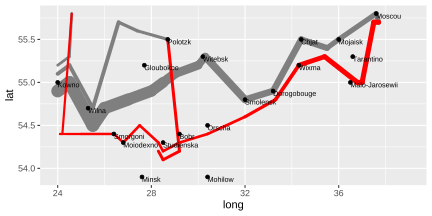
\includegraphics{tools_files/figure-latex/ggplot2-minard-1} 

}

\caption[在 R 中用 \textbf{ggplot2} 包重制拿破仑远征图]{在 R 中用 \textbf{ggplot2} 包重制拿破仑远征图:我们可以对比图 \ref{fig:minard}。}\label{fig:ggplot2-minard}
\end{figure}

\section{思考与练习}\label{ux601dux8003ux4e0eux7ec3ux4e60-1}

\begin{enumerate}
\def\labelenumi{\arabic{enumi}.}
\item
  大多数开源软件都会特别强调说明 ABSOLUTELY NO WARRANTY,这是否让你感到开源软件质量没有保证?CRAN 上的 R 包已经数以千计,而这些用户贡献的附加包几乎都是没有人去检查质量好坏(服务器上只做一些例行检查如是否有语法错误),我们应该以什么样的原则去使用附加包?盲目信任、完全摒弃或者自行测试?
\item
  统计图形和统计计算有怎样的联系?
\end{enumerate}

\chapter{元素}\label{cha:elements}

\begin{quote}
他从信封里拿出一页四折叠的半张 \(13\times17\) 英寸的信纸。他把信纸打开铺在桌上,中间有一行铅字拼贴成的句子:

若你看重自己生命的价值或还有理性,那就远离沼地。

只有``沼地''两个字是用墨水写的。

``现在,''亨利·巴斯克维尔爵士说,``福尔摩斯先生,也许您可以告诉我,这是什么意思,到底是谁对我的事这么感兴趣呢?''

\ldots\ldots{}``可是,亲爱的华生,两者之间的联系非常紧密,短信中的每个单字都是从这个长句中抽出来的。例如:`你'、`你的'、`生'、`命'、`理性'、`价值'、'远离'等,你现在还看不出这些字是从那里面弄来的吗?''

``天啊!太对了!唉呀,您可聪明绝顶!''亨利爵士喊了起来。

\hspace*{\fill} --- 柯南·道尔《巴斯克维尔的猎犬》
\end{quote}

任何一幅统计图形都是由最基础的图形元素构成的,这些元素我们并不陌生,无非就是颜色、点、线(直线、曲线、线段甚至箭头)、矩形、任意多边形、文本以及图例。R 提供了相应的一系列函数,用以向已有的图形中添加图形元素。事实上,R 的所有作图函数分为两类,一类是高层函数(high-level),用以生成新的图形;另一类就是低层函数(low-level),这一类指的正是绘制图形元素的这些基础函数。

本章所介绍的图形元素都是基础图形系统的元素,关于其它系统的元素,参见第 \ref{chap:system} 章,但归根结底,构建图形的原理是类似的。本章的目的是让读者了解如何从底层一步步构造一幅完整图形。当然,这并非对所有读者都有用,若想直接了解 R 高层作图函数,不妨直接跳入第 \ref{cha:gallery} 章。

\section{颜色}\label{sec:color}

默认情况下,R 中颜色的设置主要需要依靠 \textbf{grDevices} 包的支持,其中提供了大量的颜色选择函数和生成函数,以及几种预先设置好的调色板(Palette),用以表现不同的主题。我们把 \textbf{grDevices} 包中所有关于颜色的函数大致分为三类:固定颜色选择函数、颜色生成和转换函数、特定颜色主题调色板,这些函数将在下面三小节中详细介绍。

\subsection{固定颜色选择函数}\label{sec:palette}

固定颜色选择函数也就是 R 提供的它自带固定种类的颜色,主要是函数 \texttt{colors()} 以及 \texttt{palette()}:

\begin{description}
\tightlist
\item[\texttt{colors(),\ colours()}]
这两个函数完全一样,只是英文的两种不同拼写而已,它们不需要任何参数,会生成 657 种颜色名称,如:\texttt{\textquotesingle{}beige\textquotesingle{}}(米色)、 \texttt{\textquotesingle{}bisque\textquotesingle{}}(桔黄色)、\texttt{\textquotesingle{}chocolate\textquotesingle{}}(巧克力色)、\texttt{\textquotesingle{}cyan\textquotesingle{}}(青色)、\texttt{\textquotesingle{}gold\textquotesingle{}}(金黄色)、 \texttt{\textquotesingle{}ivory\textquotesingle{}}(象牙色)、\texttt{\textquotesingle{}lavender\textquotesingle{}}(浅紫色)等。下面的代码表示从 \texttt{colors()} 中随机抽取 20 种颜色(注意,\texttt{sample()} 是随机抽样函数,因此重复这个语句每次得到的结果可能会不一样,这是正常的):
\end{description}

\begin{Shaded}
\begin{Highlighting}[]
\FunctionTok{sample}\NormalTok{(}\FunctionTok{colors}\NormalTok{(), }\DecValTok{20}\NormalTok{)}
\end{Highlighting}
\end{Shaded}

\begin{verbatim}
##  [1] "skyblue"         "grey61"          "goldenrod3"      "turquoise4"     
##  [5] "lightsteelblue2" "gray68"          "navajowhite1"    "grey72"         
##  [9] "mistyrose1"      "greenyellow"     "darkolivegreen1" "burlywood4"     
## [13] "dodgerblue1"     "honeydew"        "darkseagreen4"   "grey0"          
## [17] "cornflowerblue"  "dodgerblue3"     "darkseagreen3"   "firebrick4"
\end{verbatim}

有兴趣观看所有 657 种颜色的读者可以试着运行下面的语句,其中 \texttt{pdf()} 函数的作用是打开一个作图设备,详情参见附录 \ref{sec:device} 节,可以把参数 \texttt{\textquotesingle{}colors-bar.pdf\textquotesingle{}} 替换为任意一个可以读写的路径 \footnote{Windows 用户注意路径的写法,不能用通常的单反斜杠 \textbackslash,而应该把路径中的单反斜杠换成双反斜杠 \textbackslash\textbackslash{} 或者用单斜杠 /;如 \texttt{D:/colors.pdf} 或 \texttt{D:\textbackslash{}\textbackslash{}colors.pdf}},条形图 \texttt{barplot()} 的说明参见 \ref{sec:barplot} 小节。最后结果是在设定文件路径上获得一个 PDF 文件,展示所有颜色名称及其对应的颜色。

\begin{Shaded}
\begin{Highlighting}[]
\FunctionTok{pdf}\NormalTok{(}\StringTok{"colors{-}bar.pdf"}\NormalTok{, }\AttributeTok{height =} \DecValTok{120}\NormalTok{)}
\FunctionTok{par}\NormalTok{(}\AttributeTok{mar =} \FunctionTok{c}\NormalTok{(}\DecValTok{0}\NormalTok{, }\DecValTok{10}\NormalTok{, }\DecValTok{3}\NormalTok{, }\DecValTok{0}\NormalTok{) }\SpecialCharTok{+} \FloatTok{0.1}\NormalTok{, }\AttributeTok{yaxs =} \StringTok{"i"}\NormalTok{)}
\FunctionTok{barplot}\NormalTok{(}\FunctionTok{rep}\NormalTok{(}\DecValTok{1}\NormalTok{, }\FunctionTok{length}\NormalTok{(}\FunctionTok{colors}\NormalTok{())),}
  \AttributeTok{col =} \FunctionTok{rev}\NormalTok{(}\FunctionTok{colors}\NormalTok{()), }\AttributeTok{names.arg =} \FunctionTok{rev}\NormalTok{(}\FunctionTok{colors}\NormalTok{()), }\AttributeTok{horiz =} \ConstantTok{TRUE}\NormalTok{,}
  \AttributeTok{las =} \DecValTok{1}\NormalTok{, }\AttributeTok{xaxt =} \StringTok{"n"}\NormalTok{, }\AttributeTok{main =} \FunctionTok{expression}\NormalTok{(}\StringTok{"Bars of colors in"} \SpecialCharTok{\textasciitilde{}} \FunctionTok{italic}\NormalTok{(}\FunctionTok{colors}\NormalTok{()))}
\NormalTok{)}
\FunctionTok{dev.off}\NormalTok{()}
\end{Highlighting}
\end{Shaded}

\begin{description}
\tightlist
\item[\texttt{palette()}]
调色板函数;用法 \texttt{palette(value)},这个函数用来设置调色板或者获得调色板颜色值;注意,实际上这个函数的结果可能并非``固定''颜色,但是只要设定好了调色板,它的取值就不会再改变(直到下一次重新设定调色板)。如果不写任何参数,那么该函数返回当前的调色板设置,即一个包含当前调色板中所有颜色的向量;若参数长度为 1 则将当前调色板重新设置为以该参数为名称的调色板,目前这种参数只有 \texttt{\textquotesingle{}default\textquotesingle{}} 这一种,即设置为默认调色板:\texttt{palette(\textquotesingle{}default\textquotesingle{})};若参数为一个颜色向量,那么将当前调色板中的颜色更改为该参数表示的颜色。如下例:
\end{description}

\begin{Shaded}
\begin{Highlighting}[]
\FunctionTok{palette}\NormalTok{() }\CommentTok{\# 默认的调色板颜色}
\end{Highlighting}
\end{Shaded}

\begin{verbatim}
## [1] "black"   "#DF536B" "#61D04F" "#2297E6" "#28E2E5" "#CD0BBC" "#F5C710"
## [8] "gray62"
\end{verbatim}

\begin{Shaded}
\begin{Highlighting}[]
\FunctionTok{palette}\NormalTok{(}\FunctionTok{colors}\NormalTok{()[}\DecValTok{1}\SpecialCharTok{:}\DecValTok{10}\NormalTok{]) }\CommentTok{\# 重新设置调色板为 colors() 的前 10 种颜色}
\FunctionTok{palette}\NormalTok{() }\CommentTok{\# 更改后的调色板颜色}
\end{Highlighting}
\end{Shaded}

\begin{verbatim}
##  [1] "white"         "aliceblue"     "antiquewhite"  "antiquewhite1"
##  [5] "antiquewhite2" "antiquewhite3" "antiquewhite4" "aquamarine"   
##  [9] "aquamarine"    "aquamarine2"
\end{verbatim}

\begin{Shaded}
\begin{Highlighting}[]
\FunctionTok{palette}\NormalTok{(}\StringTok{"default"}\NormalTok{) }\CommentTok{\# 恢复默认调色板}
\end{Highlighting}
\end{Shaded}

调色板的好处在于,我们可以在 R 中使用一个整数来表示颜色,而这个整数对应的颜色就是调色板中相应位置的颜色,比如在某作图函数中调用参数 \texttt{col\ =\ 2} 表示取调色板中第 2 种颜色。 若整数值超过了调色板颜色向量的长度,那么 R 会自动取该整数除以调色板颜色向量长度的余数。

\subsection{颜色生成和转换函数}\label{ux989cux8272ux751fux6210ux548cux8f6cux6362ux51fdux6570}

R 提供了一系列利用颜色生成模型如 RGB 模型(红绿蓝三原色混合)、HSV 色彩模型(色调、饱和度和纯度)、HCL 色彩模型(色调、色度和亮度)和灰色生成模型等。颜色的构造原理比较复杂,超出了本书讨论范围,因此这里仅对相关函数的用法作介绍。

\begin{description}
\tightlist
\item[\texttt{rgb()}]
红绿蓝三原色混合,用法 \texttt{rgb(red,\ green,\ blue,\ alpha,\ names\ =\ NULL,\ maxColorValue\ =\ 1)};其中前四个参数都取值于区间 {[}0, maxColorValue{]},\texttt{names} 参数用来指定生成颜色向量的名称。这里前三个参数不用过多解释,值越大就说明那种颜色的成分越高;可能 \texttt{alpha} 我们不太熟悉,它指的是颜色的透明度,取 0 表示完全透明,取最大值表示完全不透明(默认),透明度在统计图形中有着重要地位,因为它具有一个非常有用的性质 --- 透明度可以叠加,即:两个或多个带有透明色的图形元素重叠在一起时,重叠部分的透明度会变小;这在某些统计图形中可以找到很好的应用,例如当散点图中点的数目过多而导致大量的点相互重叠时,我们可以使用透明色来看清图中的深层规律,其中一个直接的规律就是二维密度,点重叠越密集,则颜色越深(由于透明度的的叠加),该处的密度值也越大,图 \ref{fig:scatter-alpha} 给出了一个半透明色应用的示例。
\item[\texttt{hsv()}]
用色调(Hue)、饱和度(Saturation)和纯度(Value)来构造颜色,用法 \texttt{hsv(h\ =\ 1,\ s\ =\ 1,\ v\ =\ 1,\ alpha)};前三个参数分别对应色调、饱和度和纯度,取值于区间 \([0, 1]\);\texttt{alpha} 意思同上,但取值于区间 \([0, 1]\)
\item[\texttt{hcl()}]
用色调(Hue)、色度(Chroma)和亮度(Luminance)构造颜色,用法为 \texttt{hcl(h\ =\ 0,\ c\ =\ 35,\ l\ =\ 85,\ alpha,\ fixup\ =\ TRUE)};参数 h 取值于区间 \([0, 360]\),可以将它想象为一个角度:\(0\,^{\circ}\) 表示红色,\(120\,^{\circ}\) 表示绿色,\(240\,^{\circ}\) 表示蓝色,中间的都是过渡色;参数 \texttt{c} 取值受 \texttt{h} 和 \texttt{l} 限制;参数 \texttt{l} 取值在区间 \([0, 100]\) 上,取值越大生成的颜色越亮;\texttt{alpha} 意思同 \texttt{hsv()};\texttt{fixup} 表示是否修正生成的颜色值,之所以要修正,是因为有些搭配生成的 RGB 颜色 \texttt{(r,\ g,\ b)} 可能出现某一个元素超过 1 的情形
\item[\texttt{gray(),\ grey()}]
生成灰色系列;只有一个参数 \texttt{level},表示灰度水平,取值在 0 到 1 之间,其中 0 表示纯黑色,而 1 表示纯白色;\texttt{level} 取一个向量则可以生成一系列灰色值,如下例:
\end{description}

\begin{Shaded}
\begin{Highlighting}[]
\FunctionTok{gray}\NormalTok{(}\FunctionTok{seq}\NormalTok{(}\DecValTok{0}\NormalTok{, }\DecValTok{1}\NormalTok{, }\AttributeTok{length =} \DecValTok{5}\NormalTok{))}
\end{Highlighting}
\end{Shaded}

\begin{verbatim}
## [1] "#000000" "#404040" "#808080" "#BFBFBF" "#FFFFFF"
\end{verbatim}

熟悉十六进制的人应该能看出这些颜色都是由六个十六进制数字组成的,每两位数字(合起来取值从 0 到 255)分别表示红绿蓝(RGB 颜色)的比例。我们知道,当三原色完全混合时,生成的颜色是白色,上面结果的最后一个 \texttt{\textquotesingle{}\#FFFFFF\textquotesingle{}} 正是纯白色。

除了颜色生成函数之外,\textbf{grDevices} 包还提供了两种颜色转换函数,作用就是把一种颜色从一种颜色系统空间转移到另一种颜色系统空间中表示。这两个函数分别是:

\begin{description}
\tightlist
\item[\texttt{rgb2hsv()}]
将 RGB 颜色转换为 HSV 颜色,用法 \texttt{rgb2hsv(r,\ g\ =\ NULL,\ b\ =\ NULL,\ maxColorValue\ =\ 255)};所有参数意思已经在上面的列表中解释过,只是要注意,当 \texttt{r} 是一个矩阵时,另外两个参数 \texttt{g} 和 \texttt{b} 就应省略不写。下例中我们将一个 \(3\times4\) 的 RGB 颜色矩阵传入函数 \texttt{rgb2hsv()},该函数会把每一列 RGB 颜色都转化为相应的 HSV 颜色。颜色矩阵的前三列分别是红、绿和蓝色,请观察和对比两种颜色系统的表示方法。
\end{description}

\begin{Shaded}
\begin{Highlighting}[]
\CommentTok{\# 赋值给变量 rgb.mat}
\NormalTok{(rgb.mat }\OtherTok{\textless{}{-}} \FunctionTok{matrix}\NormalTok{(}\FunctionTok{c}\NormalTok{(}\DecValTok{255}\NormalTok{, }\DecValTok{0}\NormalTok{, }\DecValTok{0}\NormalTok{, }\DecValTok{0}\NormalTok{, }\DecValTok{255}\NormalTok{, }\DecValTok{0}\NormalTok{, }\DecValTok{0}\NormalTok{, }\DecValTok{0}\NormalTok{, }\DecValTok{255}\NormalTok{, }\DecValTok{10}\NormalTok{, }\DecValTok{100}\NormalTok{, }\DecValTok{200}\NormalTok{), }\AttributeTok{nrow =} \DecValTok{3}\NormalTok{))}
\end{Highlighting}
\end{Shaded}

\begin{verbatim}
##      [,1] [,2] [,3] [,4]
## [1,]  255    0    0   10
## [2,]    0  255    0  100
## [3,]    0    0  255  200
\end{verbatim}

\begin{Shaded}
\begin{Highlighting}[]
\FunctionTok{rgb2hsv}\NormalTok{(rgb.mat)}
\end{Highlighting}
\end{Shaded}

\begin{verbatim}
##   [,1]      [,2]      [,3]      [,4]
## h    0 0.3333333 0.6666667 0.5877193
## s    1 1.0000000 1.0000000 0.9500000
## v    1 1.0000000 1.0000000 0.7843137
\end{verbatim}

\begin{description}
\tightlist
\item[\texttt{col2rgb()}]
将任意一种 R 颜色值转换为 RGB 表示,用法 \texttt{col2rgb(col,\ alpha\ =\ FALSE)};参数 \texttt{col} 的取值可以有三种形式,第一种是 \texttt{colors()} 函数中的任意一种颜色名称(字符串),第二种是如 \texttt{\#rrggbb} 十六进制形式的的 RGB 颜色表示,第三种是一个整数,即调色板中相应位置的颜色。
\end{description}

\begin{Shaded}
\begin{Highlighting}[]
\FunctionTok{col2rgb}\NormalTok{(}\DecValTok{4}\NormalTok{) }\CommentTok{\# 调色板中第 4 种颜色默认是蓝色}
\end{Highlighting}
\end{Shaded}

\begin{verbatim}
##       [,1]
## red     34
## green  151
## blue   230
\end{verbatim}

\begin{Shaded}
\begin{Highlighting}[]
\FunctionTok{col2rgb}\NormalTok{(}\StringTok{"yellow"}\NormalTok{) }\CommentTok{\# 黄色是由红绿混合得到的}
\end{Highlighting}
\end{Shaded}

\begin{verbatim}
##       [,1]
## red    255
## green  255
## blue     0
\end{verbatim}

\begin{Shaded}
\begin{Highlighting}[]
\FunctionTok{col2rgb}\NormalTok{(}\StringTok{"\#FF00FF"}\NormalTok{) }\CommentTok{\# 红蓝混合为紫色}
\end{Highlighting}
\end{Shaded}

\begin{verbatim}
##       [,1]
## red    255
## green    0
## blue   255
\end{verbatim}

\subsection{特定颜色主题调色板}\label{subsec:palette}

前面介绍的颜色生成过程对于一般人来说也许显得太复杂,除了美术和绘图专业人士,大部分人可能并不懂颜色的透明度、饱和度等概念,那么在配制大批量颜色的时候可能会比较迷惑。此时,R 提供了第三种选择,那就是特定颜色主题的调色板。这些调色板都用一系列渐变的颜色表现了特定的主题,例如彩虹颜色系列、白热化颜色系列、地形颜色系列等等。

\begin{description}
\tightlist
\item[\texttt{rainbow()}]
顾名思义,就是用彩虹的颜色(``红橙黄绿青蓝紫'')来产生一系列颜色,用法 \texttt{rainbow(n,\ s\ =\ 1,\ v\ =\ 1,\ start\ =\ 0,\ end\ =\ max(1,\ n\ -\ 1)/n)};参数 \texttt{n} 设定产生颜色的数目,参数 \texttt{s}、\texttt{v} 前文已经解释过;参数 \texttt{start} 和 \texttt{end} 设定彩虹颜色的一个子集,生成的颜色将从这个子集中选取,这个子集选取的大致分界线为:红色(red)为 0,黄色(yellow)为 1/6,绿色(green)为 2/6,青色(cyan)为 3/6,蓝色(blue)为 4/6,红紫色(magenta)为 5/6
\item[\texttt{heat.colors()}]
从红色渐变到黄色再变到白色(以体现``高温''、``白热化'',读者可以在 R 中运行 \texttt{demo(image)} 并观察第二幅等高线图)
\item[\texttt{terrain.colors()}]
从绿色渐变到黄色再到棕色最后到白色(这些颜色适合表示地理地形,读者可以运行 \texttt{demo(persp)} 并观察最后两幅关于火山的三维图形,以及运行 \texttt{demo(image)} 并观察第一幅等高线图)
\item[\texttt{topo.colors()}]
从蓝色渐变到青色再到黄色最后到棕色
\item[\texttt{cm.colors()}]
从青色渐变到白色再到粉红色(读者可以运行 \texttt{demo(image)} 并观察最后几幅颜色图)
\end{description}

若想要获得更复杂更精细的颜色或调色板,不妨使用 \textbf{grDevices} 包中的颜色``插值''函数,如 \texttt{colorRamp()} 和 \texttt{colorRampPalette()} 函数,读者可以根据需要产生符合特定要求的调色板,以适应展示主题的需要,这里不详述这两个函数的使用方法。

对于缺乏耐心和兴趣去研究颜色的用户来说,附加包 \textbf{RColorBrewer}\citep{RColorBrewer} 也不失为一个好的选择。这个包提供了三类调色板,用户只需要指定调色板名称,就可以用包中的 \texttt{brewer.pal()} 函数生成颜色。这三类调色板包括:

\begin{description}
\tightlist
\item[连续型调色板 Sequential palettes]
生成一系列连续渐变的颜色,通常用来标记连续型数值的大小
\item[极端化调色板 Diverging palettes]
生成用深色强调两端、浅色标示中部的系列颜色,可用来标记数据中的离群点
\item[离散型调色板 Qualitative palettes]
生成一系列彼此差异比较明显的颜色,通常用来标记分类数据
\end{description}

每一类调色板下有若干种具体的实现,例如 Blues 是连续型调色板下的一种,用以蓝色主题的渐变颜色:

\begin{Shaded}
\begin{Highlighting}[]
\FunctionTok{library}\NormalTok{(RColorBrewer)}
\FunctionTok{brewer.pal}\NormalTok{(}\DecValTok{9}\NormalTok{, }\StringTok{"Blues"}\NormalTok{)}
\end{Highlighting}
\end{Shaded}

\begin{verbatim}
## [1] "#F7FBFF" "#DEEBF7" "#C6DBEF" "#9ECAE1" "#6BAED6" "#4292C6" "#2171B5"
## [8] "#08519C" "#08306B"
\end{verbatim}

所有调色板名称及其展示参见图 \ref{fig:ColorBrewer-all}。这些调色板并非一些简单的颜色组合,而是有一定科学根据的。例如离散型调色板下的颜色对大多数人来说都有较好的区分度,甚至色盲也可以辨认其中不同类的颜色。如果用户对颜色选取拿捏不准,不妨用这个包来生成颜色。实际上这个 R 包是一款叫 ColorBrewer 的产品的重新实现,更多信息可以访问网站 \url{http://colorbrewer2.org/}。

\begin{Shaded}
\begin{Highlighting}[]
\FunctionTok{layout}\NormalTok{(}\FunctionTok{matrix}\NormalTok{(}\DecValTok{1}\SpecialCharTok{:}\DecValTok{3}\NormalTok{, }\DecValTok{3}\NormalTok{), }\AttributeTok{heights =} \FunctionTok{c}\NormalTok{(}\DecValTok{2}\NormalTok{, }\DecValTok{1}\NormalTok{, }\DecValTok{1}\NormalTok{))}
\FunctionTok{par}\NormalTok{(}\AttributeTok{mar =} \FunctionTok{c}\NormalTok{(}\DecValTok{0}\NormalTok{, }\DecValTok{4}\NormalTok{, }\DecValTok{0}\NormalTok{, }\DecValTok{0}\NormalTok{))}
\FunctionTok{display.brewer.all}\NormalTok{(}\AttributeTok{type =} \StringTok{"seq"}\NormalTok{) }\CommentTok{\# 连续型:18 种}
\FunctionTok{display.brewer.all}\NormalTok{(}\AttributeTok{type =} \StringTok{"div"}\NormalTok{) }\CommentTok{\# 极端化:9 种}
\FunctionTok{display.brewer.all}\NormalTok{(}\AttributeTok{type =} \StringTok{"qual"}\NormalTok{) }\CommentTok{\# 离散型:8 种}
\end{Highlighting}
\end{Shaded}

\begin{figure}

{\centering 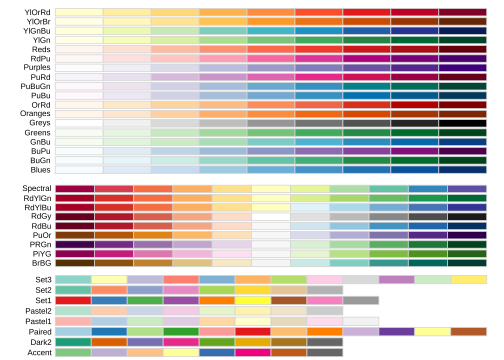
\includegraphics{elements_files/figure-latex/ColorBrewer-all-1} 

}

\caption[RColorBrewer 包中所有调色板颜色的演示 ]{RColorBrewer 包中所有调色板颜色的演示:从上至下依次是连续型、极端化和离散型调色板。}\label{fig:ColorBrewer-all}
\end{figure}



\subsection{渐变色的简单原理及应用}\label{ux6e10ux53d8ux8272ux7684ux7b80ux5355ux539fux7406ux53caux5e94ux7528}

\begin{Shaded}
\begin{Highlighting}[]
\NormalTok{xx }\OtherTok{\textless{}{-}} \FunctionTok{c}\NormalTok{(}\DecValTok{1912}\NormalTok{, }\DecValTok{1912}\SpecialCharTok{:}\DecValTok{1971}\NormalTok{, }\DecValTok{1971}\NormalTok{)}
\NormalTok{yy }\OtherTok{\textless{}{-}} \FunctionTok{c}\NormalTok{(}\FunctionTok{min}\NormalTok{(nhtemp), nhtemp, }\FunctionTok{min}\NormalTok{(nhtemp))}
\FunctionTok{plot}\NormalTok{(xx, yy, }\AttributeTok{type =} \StringTok{"n"}\NormalTok{, }\AttributeTok{xlab =} \StringTok{"Year"}\NormalTok{, }\AttributeTok{ylab =} \StringTok{"Temperatures"}\NormalTok{)}
\ControlFlowTok{for}\NormalTok{ (i }\ControlFlowTok{in} \FunctionTok{seq}\NormalTok{(}\DecValTok{255}\NormalTok{, }\DecValTok{0}\NormalTok{, }\SpecialCharTok{{-}}\DecValTok{3}\NormalTok{)) \{}
\NormalTok{  yy }\OtherTok{\textless{}{-}} \FunctionTok{c}\NormalTok{(}\DecValTok{45}\NormalTok{, nhtemp }\SpecialCharTok{{-}}\NormalTok{ (nhtemp }\SpecialCharTok{{-}} \FunctionTok{min}\NormalTok{(nhtemp)) }\SpecialCharTok{*}\NormalTok{ (}\DecValTok{1} \SpecialCharTok{{-}}\NormalTok{ i }\SpecialCharTok{/} \DecValTok{255}\NormalTok{), }\DecValTok{45}\NormalTok{) }\CommentTok{\# rgb() 中的绿色成分逐渐变小}
  \FunctionTok{polygon}\NormalTok{(xx, yy, }\AttributeTok{col =} \FunctionTok{rgb}\NormalTok{(}\DecValTok{1}\NormalTok{, i }\SpecialCharTok{/} \DecValTok{255}\NormalTok{, }\DecValTok{0}\NormalTok{), }\AttributeTok{border =} \ConstantTok{NA}\NormalTok{)}
  \CommentTok{\# 读者可以在这里加上 Sys.sleep(0.05) 以便看清作图过程}
\NormalTok{\}}
\FunctionTok{box}\NormalTok{() }\CommentTok{\# 补齐边框}
\end{Highlighting}
\end{Shaded}

\begin{figure}

{\centering 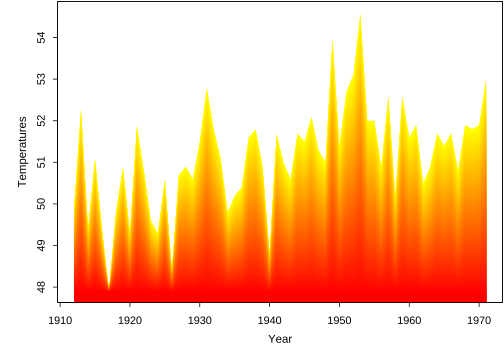
\includegraphics{elements_files/figure-latex/grad-color-1} 

}

\caption[New Haven 地区的年均气温(1912~1971 年)]{New Haven 地区的年均气温(1912\textasciitilde1971 年):统计图形的应用应该根据数据和事实的环境灵活选取图形的样式。本图的数据为 1912 年至 1971 年 New Haven 地区的年均气温。数据来源:\textbf{datasets} 包中的 nhtemp。}\label{fig:grad-color}
\end{figure}



在此我们特别用一节来讲述``渐变色'',原因在于在图形中应用渐变色往往能让图形看起来更美观、避免单调的颜色在图形中显得突兀。不难想象,所谓``渐变'',也就是逐渐变化的意思,这种变化必然对应着某种单调或非单调的(可导)函数,这些函数用来控制颜色值逐步变化。最简单的例子莫过于线性函数:从一种颜色值到另一种颜色值线性变化。比如我们在 \texttt{rgb()} 函数中用一元线性函数控制绿色在 \([0, 1]\) 上的取值,同时将红色和蓝色分别控制为 1 和 0, 那么我们将得到从纯红色到黄色的一个颜色渐变。如:

\begin{Shaded}
\begin{Highlighting}[]
\NormalTok{(x }\OtherTok{\textless{}{-}} \FunctionTok{rgb}\NormalTok{(}\DecValTok{1}\NormalTok{, }\FunctionTok{seq}\NormalTok{(}\DecValTok{0}\NormalTok{, }\DecValTok{1}\NormalTok{, }\AttributeTok{length =} \DecValTok{30}\NormalTok{), }\DecValTok{0}\NormalTok{))}
\end{Highlighting}
\end{Shaded}

\begin{verbatim}
##  [1] "#FF0000" "#FF0900" "#FF1200" "#FF1A00" "#FF2300" "#FF2C00" "#FF3500"
##  [8] "#FF3E00" "#FF4600" "#FF4F00" "#FF5800" "#FF6100" "#FF6A00" "#FF7200"
## [15] "#FF7B00" "#FF8400" "#FF8D00" "#FF9500" "#FF9E00" "#FFA700" "#FFB000"
## [22] "#FFB900" "#FFC100" "#FFCA00" "#FFD300" "#FFDC00" "#FFE500" "#FFED00"
## [29] "#FFF600" "#FFFF00"
\end{verbatim}

\begin{Shaded}
\begin{Highlighting}[]
\CommentTok{\# 读者不妨用 barplot(rep(1, 30), col = x) 看看效果}
\end{Highlighting}
\end{Shaded}

显然本小节的内容与前一小节所讲到的调色板是一致的,只不过调色板是预先配置好了的渐变色系列;我们在这里``重复''讲述渐变色的简单原理,目的是尽量让读者了解各种看起来比较神秘和高深的颜色使用招数的本质。

在本节的最后,我们要再次强调颜色的艺术性:根据不同的环境选用不同的颜色。虽然统计专业人士对绘画、美学可能不必深入了解,但是漂亮、适宜的统计图形总是受人欢迎的。作者曾经在 \href{https://www.stat.auckland.ac.nz/~ihaka/}{Ross Ihaka} 的个人主页上看到一个很好的例子,内容是展示全球气候变暖的温度随年份变化的折线图,这幅图使用了从黄色到红色的渐变色,而这样的颜色恰好能体现温度的灼热感,对于警示温室效应来说,这种渐变色是极为恰当的(思考一下我们平时作折线图是否会考虑这样的颜色搭配);Ross Ihaka 并没有给出具体的代码,但通过前面的介绍和后面 \ref{sec:polygon} 小节的阅读,相信读者一定可以自己动手作出类似的折线图。这里我们也给出一段示例代码,核心部分在于控制多边形的 \texttt{col} 参数;事实上,这幅``折线图''是由多个颜色渐变的多边形重叠而成的,效果见图 \ref{fig:grad-color}(图中数据为真实气温数据)。

\section{点}\label{sec:points}

关于点的设置,我们既可以在很多作图函数中用 \texttt{pch} 等参数实现,也可以在用低层函数 \texttt{points()} 向已有图形中添加点来实现。后一种方法往往更灵活自由。\texttt{points()} 用法:

\begin{Shaded}
\begin{Highlighting}[]
\FunctionTok{usage}\NormalTok{(points, }\StringTok{"default"}\NormalTok{)}
\end{Highlighting}
\end{Shaded}

\begin{verbatim}
## points(x, ...)
\end{verbatim}

函数 \texttt{points()} 的参数如 \texttt{pch} 和 \texttt{col} 等在 \ref{sec:par} 小节介绍 \texttt{par()} 函数时中有详细解释,但这两个函数中相同名称的参数最主要的一点区别就是,前者可以使用向量,而后者只能接受一个单值作为参数。此外还有一点细小差异在于参数 \texttt{bg},它在函数 \texttt{points()} 中表示的是点的背景色而非图形的背景色。为了向图中添加一系列不同样式的点,我们可以使用向量作为 \texttt{points()} 的参数。

\begin{Shaded}
\begin{Highlighting}[]
\FunctionTok{demo}\NormalTok{(}\StringTok{"pointTypes"}\NormalTok{, }\AttributeTok{package =} \StringTok{"MSG"}\NormalTok{)}
\end{Highlighting}
\end{Shaded}

\begin{figure}

{\centering 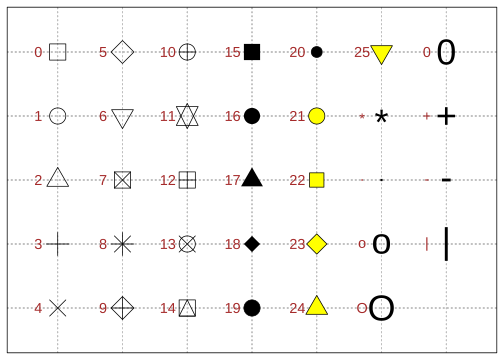
\includegraphics{elements_files/figure-latex/point-type-1} 

}

\caption[点的类型:\texttt{pch} 参数取值从 0 到 25 及其它符号]{点的类型:\texttt{pch} 参数取值从 1 到 25 及其它符号。注意:21\textasciitilde25 的点可以填充背景颜色。}\label{fig:point-type}
\end{figure}





本节不再赘述参数的意思(读者可以自行查阅帮助),但有三点仍需特别说明一下。首先是 \texttt{lwd} 参数,我们知道这是设定线条宽度的,对于点来说,这个参数同样可以设置点的边缘``线条''宽度;其次,\texttt{pch} 参数同样可以接受字符作为参数值,而不仅仅是数字;最后,参数 \texttt{pch} 取值从 21\textasciitilde25 的点可以填充背景颜色。注意观察,图 \ref{fig:point-type} 中 21\textasciitilde25 的点边缘线颜色和背景色是不同的,而在 25 之后的点则采用了文本符号作为参数 \texttt{pch} 的值。图 \ref{fig:point-type} 中也有几对形状一样的点,但是它们实质上是不一样的,例如 0、15 和 22 对应的点都是正方形,但前二者分别是空心正方形和实心正方形,且都不可填充背景,而 22 对应的点是空心正方形,可以填充背景。

一次性作出不同样式的点对于图形阅读和统计分析来说是很有利的,比如有时候我们可以把样本根据某一特征分为几组,对每一组子样本都采用不同的样式作点图,那么我们或许可以从图中点的散布情况发现组间的差异特征。图 \ref{fig:point-iris} 给出了一个鸢尾花散点图的示例(注意向量的使用),很明显,setosa 这一类花的型号较小,因为它们都处于散点图的左下角。

\begin{Shaded}
\begin{Highlighting}[]
\CommentTok{\# 先将鸢尾花的类型转化为整数 1、2、3,便于使用向量}
\NormalTok{idx }\OtherTok{\textless{}{-}} \FunctionTok{as.integer}\NormalTok{(iris[[}\StringTok{"Species"}\NormalTok{]])}
\FunctionTok{plot}\NormalTok{(iris[, }\DecValTok{3}\SpecialCharTok{:}\DecValTok{4}\NormalTok{],}
  \AttributeTok{pch =} \FunctionTok{c}\NormalTok{(}\DecValTok{24}\NormalTok{, }\DecValTok{21}\NormalTok{, }\DecValTok{25}\NormalTok{)[idx],}
  \AttributeTok{col =} \FunctionTok{c}\NormalTok{(}\StringTok{"black"}\NormalTok{, }\StringTok{"red"}\NormalTok{, }\StringTok{"blue"}\NormalTok{)[idx], }\AttributeTok{panel.first =} \FunctionTok{grid}\NormalTok{()}
\NormalTok{)}
\FunctionTok{legend}\NormalTok{(}\StringTok{"topleft"}\NormalTok{,}
  \AttributeTok{legend =} \FunctionTok{levels}\NormalTok{(iris[[}\StringTok{"Species"}\NormalTok{]]),}
  \AttributeTok{col =} \FunctionTok{c}\NormalTok{(}\StringTok{"black"}\NormalTok{, }\StringTok{"red"}\NormalTok{, }\StringTok{"blue"}\NormalTok{), }\AttributeTok{pch =} \FunctionTok{c}\NormalTok{(}\DecValTok{24}\NormalTok{, }\DecValTok{21}\NormalTok{, }\DecValTok{25}\NormalTok{), }\AttributeTok{bty =} \StringTok{"n"}
\NormalTok{)}
\end{Highlighting}
\end{Shaded}

\begin{figure}

{\centering 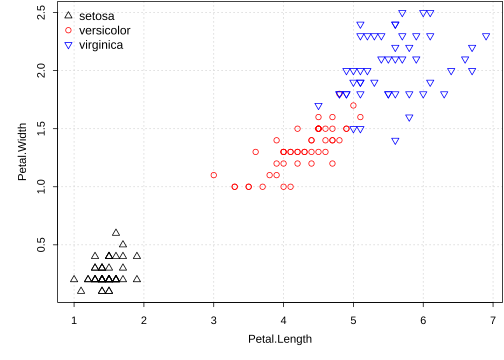
\includegraphics{elements_files/figure-latex/point-iris-1} 

}

\caption[鸢尾花的花瓣长宽散点图 ]{鸢尾花的花瓣长宽散点图:我们可以给每一种鸢尾花标记不同类型的点和颜色,这样可以帮助我们更清楚地区分鸢尾花类型。}\label{fig:point-iris}
\end{figure}

图 \ref{fig:point-random} 为本书的一例``彩蛋'':基于随机性的图形可能会具有某种艺术性。这里仅仅展示了四幅可能的输出,其它更多可能的结果参见:\url{https://yihui.org/cn/2010/08/art-of-points-in-r/},或观看演示 \texttt{demo(\textquotesingle{}pointArts\textquotesingle{},\ package\ =\ \textquotesingle{}MSG\textquotesingle{})}。若读者感兴趣,甚至可以用 R 为自己生成一幅桌面背景图片,制作方法在前面链接中有介绍。

\begin{Shaded}
\begin{Highlighting}[]
\FunctionTok{par}\NormalTok{(}\AttributeTok{mar =} \FunctionTok{c}\NormalTok{(}\FloatTok{0.2}\NormalTok{, }\FloatTok{0.2}\NormalTok{, }\FloatTok{0.2}\NormalTok{, }\FloatTok{0.2}\NormalTok{), }\AttributeTok{mfrow =} \FunctionTok{c}\NormalTok{(}\DecValTok{2}\NormalTok{, }\DecValTok{2}\NormalTok{))}
\ControlFlowTok{for}\NormalTok{ (n }\ControlFlowTok{in} \FunctionTok{c}\NormalTok{(}\DecValTok{63}\NormalTok{, }\DecValTok{60}\NormalTok{, }\DecValTok{76}\NormalTok{, }\DecValTok{74}\NormalTok{)) \{}
  \FunctionTok{set.seed}\NormalTok{(}\DecValTok{711}\NormalTok{)}
  \FunctionTok{plot.new}\NormalTok{()}
  \FunctionTok{box}\NormalTok{()}
\NormalTok{  size }\OtherTok{\textless{}{-}} \FunctionTok{c}\NormalTok{(}\FunctionTok{replicate}\NormalTok{(n, }\DecValTok{1} \SpecialCharTok{/} \FunctionTok{rbeta}\NormalTok{(}\DecValTok{2}\NormalTok{, }\FloatTok{1.5}\NormalTok{, }\DecValTok{4}\NormalTok{)))}
\NormalTok{  center }\OtherTok{\textless{}{-}} \FunctionTok{t}\NormalTok{(}\FunctionTok{replicate}\NormalTok{(n, }\FunctionTok{runif}\NormalTok{(}\DecValTok{2}\NormalTok{)))[}\FunctionTok{rep}\NormalTok{(}\DecValTok{1}\SpecialCharTok{:}\NormalTok{n, }\AttributeTok{each =} \DecValTok{2}\NormalTok{), ]}
\NormalTok{  color }\OtherTok{\textless{}{-}} \FunctionTok{paste}\NormalTok{(}\StringTok{"\#"}\NormalTok{, }\FunctionTok{apply}\NormalTok{(}
    \FunctionTok{replicate}\NormalTok{(}\DecValTok{2} \SpecialCharTok{*}\NormalTok{ n, }\FunctionTok{sample}\NormalTok{(}\FunctionTok{c}\NormalTok{(}\DecValTok{0}\SpecialCharTok{:}\DecValTok{9}\NormalTok{, LETTERS[}\DecValTok{1}\SpecialCharTok{:}\DecValTok{6}\NormalTok{]), }\DecValTok{8}\NormalTok{, }\ConstantTok{TRUE}\NormalTok{)), }\DecValTok{2}\NormalTok{, paste,}
    \AttributeTok{collapse =} \StringTok{""}
\NormalTok{  ), }\AttributeTok{sep =} \StringTok{""}\NormalTok{)}
  \FunctionTok{points}\NormalTok{(center, }\AttributeTok{cex =}\NormalTok{ size, }\AttributeTok{pch =} \FunctionTok{rep}\NormalTok{(}\DecValTok{20}\SpecialCharTok{:}\DecValTok{21}\NormalTok{, n), }\AttributeTok{col =}\NormalTok{ color)}
\NormalTok{\}}
\end{Highlighting}
\end{Shaded}

\begin{figure}

{\centering 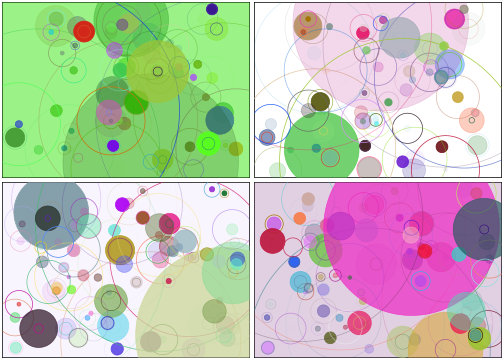
\includegraphics{elements_files/figure-latex/point-random-1} 

}

\caption[点的随机艺术作品]{点的随机艺术作品:随机生成点的大小、颜色和位置,分别用空心点和实心点画图。}\label{fig:point-random}
\end{figure}





\section{曲线、直线、线段、箭头、X-样条}\label{sec:lines}

在 \ref{sec:par} 小节介绍函数 \texttt{par()} 时我们提到了关于线条的一些参数设置,例如 \texttt{lwd} 和 \texttt{lty} 等。类似地,我们可以用函数 \texttt{lines()} 来向图中添加曲线(这里所说的曲线本质上是一些线段的连接,并非光滑的曲线);下面主要补充说明一下关于线条样式 \texttt{lty} 的设定。

R 中可以实现几乎无数种线条样式,因为它的 \texttt{lty} 参数相当灵活,除了取值 0\textasciitilde6 之外,可以根据一个十六进制的数字串(位数必须是偶数位,且非零)来设定线条的虚实,具体原理是这样:数字串的奇数位上的数字表示画相应长度的实线,然后偶数位上的数字则表示空缺相应的长度,这样就构成了一条虚线。例如,\texttt{\textquotesingle{}A5\textquotesingle{}} 表示先画 11 单位长的实线,再接着画 5 单位长的空白,紧接着又画 11 单位长的实线,\ldots\ldots,就这样重复下去,完成一条虚线;同理,\texttt{\textquotesingle{}711911\textquotesingle{}} 表示:7 单位长实线、1 单位长空白、1 单位长实线、9 单位长空白、1 单位长实线、1 单位长空白。这个十六进制的数字串的最长长度限制为 8 位。

当设定 \texttt{type\ =\ \textquotesingle{}h\textquotesingle{}} 时,\texttt{col} 参数可以使用向量,此时各条竖线都将使用不同的颜色;除此情况之外,若其它参数使用了向量,那么只有向量的第一个元素会被使用,其它元素都将被忽略掉。

\begin{Shaded}
\begin{Highlighting}[]
\CommentTok{\# 不作图,只画出框架,且指定坐标轴范围}
\FunctionTok{plot}\NormalTok{(}\DecValTok{1}\SpecialCharTok{:}\DecValTok{10}\NormalTok{, }\AttributeTok{type =} \StringTok{"n"}\NormalTok{, }\AttributeTok{xlim =} \FunctionTok{c}\NormalTok{(}\DecValTok{0}\NormalTok{, }\DecValTok{10}\NormalTok{), }\AttributeTok{ylim =} \FunctionTok{c}\NormalTok{(}\DecValTok{0}\NormalTok{, }\DecValTok{10}\NormalTok{))}
\FunctionTok{lines}\NormalTok{(}\DecValTok{1}\SpecialCharTok{:}\DecValTok{10}\NormalTok{, }\FunctionTok{abs}\NormalTok{(}\FunctionTok{rnorm}\NormalTok{(}\DecValTok{10}\NormalTok{))) }\CommentTok{\# 10 个正态随机数绝对值的波动线}
\FunctionTok{abline}\NormalTok{(}\AttributeTok{a =} \DecValTok{0}\NormalTok{, }\AttributeTok{b =} \DecValTok{1}\NormalTok{, }\AttributeTok{col =} \StringTok{"gray"}\NormalTok{) }\CommentTok{\# 不同的直线}
\FunctionTok{abline}\NormalTok{(}\AttributeTok{v =} \DecValTok{2}\NormalTok{, }\AttributeTok{h =} \DecValTok{2}\NormalTok{, }\AttributeTok{lty =} \DecValTok{2}\NormalTok{)}
\FunctionTok{text}\NormalTok{(}\DecValTok{8}\NormalTok{, }\DecValTok{3}\NormalTok{, }\StringTok{"abline(a = 0, b = 1)"}\NormalTok{) }\CommentTok{\# 添加文本}
\FunctionTok{arrows}\NormalTok{(}\DecValTok{8}\NormalTok{, }\FloatTok{3.5}\NormalTok{, }\DecValTok{6}\NormalTok{, }\FloatTok{5.7}\NormalTok{, }\AttributeTok{angle =} \DecValTok{40}\NormalTok{) }\CommentTok{\# 添加箭头}
\CommentTok{\# 参数用了向量:不同灰度的线段}
\FunctionTok{segments}\NormalTok{(}\FunctionTok{rep}\NormalTok{(}\DecValTok{3}\NormalTok{, }\DecValTok{4}\NormalTok{), }\DecValTok{6}\SpecialCharTok{:}\DecValTok{9}\NormalTok{, }\FunctionTok{rep}\NormalTok{(}\DecValTok{5}\NormalTok{, }\DecValTok{4}\NormalTok{), }\DecValTok{6}\SpecialCharTok{:}\DecValTok{9}\NormalTok{, }\AttributeTok{col =} \FunctionTok{gray}\NormalTok{(}\FunctionTok{seq}\NormalTok{(}\FloatTok{0.2}\NormalTok{, }\FloatTok{0.8}\NormalTok{, }\AttributeTok{length =} \DecValTok{4}\NormalTok{)))}
\FunctionTok{text}\NormalTok{(}\DecValTok{4}\NormalTok{, }\FloatTok{9.8}\NormalTok{, }\StringTok{"segments"}\NormalTok{)}
\end{Highlighting}
\end{Shaded}

\begin{figure}

{\centering 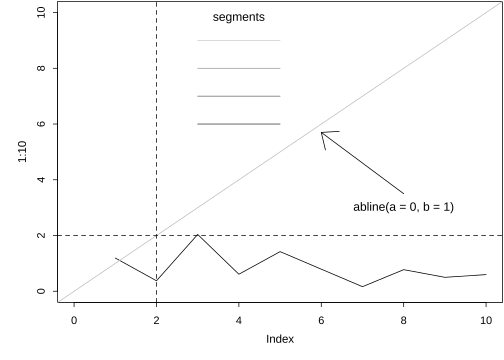
\includegraphics{elements_files/figure-latex/lines-demo-1} 

}

\caption{ 曲线、直线、直线段、箭头的展示说明 }\label{fig:lines-demo}
\end{figure}

关于直线,我们在平面坐标系中只需要确定两个因素就可以确定它的位置:即斜率和截距。函数 \texttt{abline()} 就是用来添加直线的,参数同样可以使用向量(这一点在低层函数中几乎普遍适用,所以后面不再重复说明)。函数用法如下:

\begin{Shaded}
\begin{Highlighting}[]
\FunctionTok{usage}\NormalTok{(abline)}
\end{Highlighting}
\end{Shaded}

\begin{verbatim}
## abline(a = NULL, b = NULL, h = NULL, v = NULL, reg = NULL, coef = NULL,
##   untf = FALSE, ...)
\end{verbatim}

其中,\texttt{a} 是截距,\texttt{b} 是斜率,\texttt{h} 是画水平线时的纵轴值,\texttt{v} 是画垂直线时的横轴值,\texttt{reg} 是一个能用函数 \texttt{coef()} 提取系数(包含斜率和截距)的 R 对象,典型的就是用线性模型(回归)生成的对象,系数是一个长度为 2 的向量,分别为截距和斜率;后面的 \texttt{...} 表示还可以传入其它参数(比如 \texttt{lty}、\texttt{col} 等)。

线段可以用函数 \texttt{segments()} 生成,用法如下:

\begin{Shaded}
\begin{Highlighting}[]
\FunctionTok{usage}\NormalTok{(segments)}
\end{Highlighting}
\end{Shaded}

\begin{verbatim}
## segments(x0, y0, x1 = x0, y1 = y0, col = par("fg"), lty = par("lty"),
##   lwd = par("lwd"), ...)
\end{verbatim}

前四个参数表示线段的起点和终点坐标,后面的参数相信读者也都已经熟悉。箭头可以用函数 \texttt{arrows()} 生成,用法如下:

\begin{Shaded}
\begin{Highlighting}[]
\FunctionTok{usage}\NormalTok{(arrows)}
\end{Highlighting}
\end{Shaded}

\begin{verbatim}
## arrows(x0, y0, x1 = x0, y1 = y0, length = 0.25, angle = 30, code = 2,
##   col = par("fg"), lty = par("lty"), lwd = par("lwd"), ...)
\end{verbatim}

类似于线段,前四个参数表示箭头的起点和终点坐标,\texttt{length} 表示箭头尖上短线的长度(单位:英寸),\texttt{angle} 表示箭头尖短线的角度(默认为 \(30\,^{\circ}\)),\texttt{code} 表示箭头的样式(整数 1\textasciitilde3 分别表示尾部箭头、首部箭头和两端都带箭头),注意若 \texttt{length} 设置为 0,那么将不会画出箭头(只有箭头线的主体即一条线段)。关于曲线、直线、线段和箭头函数的示例代码和效果参见图 \ref{fig:lines-demo}

\begin{Shaded}
\begin{Highlighting}[]
\FunctionTok{demo}\NormalTok{(}\StringTok{"xsplineDemo"}\NormalTok{, }\AttributeTok{package =} \StringTok{"MSG"}\NormalTok{)}
\end{Highlighting}
\end{Shaded}

\begin{figure}

{\centering 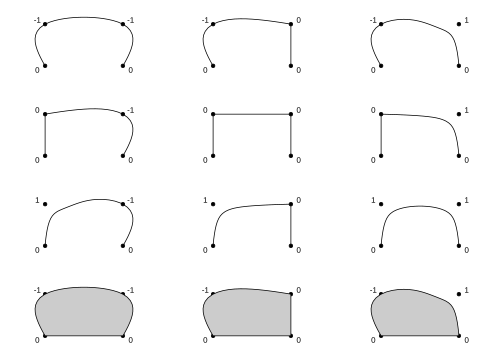
\includegraphics{elements_files/figure-latex/xspline-demo-1} 

}

\caption[X-样条各种形状的展示]{X-样条各种形状的展示:观察 \texttt{shape} 参数的取值(图中标注的数字)与样条形状的对应关系。}\label{fig:xspline-demo}
\end{figure}





下面我们再介绍一下一种特殊的曲线 --- X-样条(X-spline),样条是用光滑曲线连接若干数据点的曲线,注意它与前面提到的曲线 \texttt{lines()} 的区别在于数据点之间的连接线。样条函数用法如下:

\begin{Shaded}
\begin{Highlighting}[]
\FunctionTok{usage}\NormalTok{(xspline)}
\end{Highlighting}
\end{Shaded}

\begin{verbatim}
## xspline(x, y = NULL, shape = 0, open = TRUE, repEnds = TRUE, draw = TRUE,
##   border = par("fg"), col = NA, ...)
\end{verbatim}

前两个参数给定点的位置,\texttt{shape} 为样条的形状,取值在 \([-1, 1]\) 之间,当取值为负数时,曲线穿过给定的点,负值绝对值越小则曲线的角度越尖锐,反之角度越圆滑,\texttt{shape} 取值为正数时,曲线脱离给定的点,正值越小越靠近给定点;\texttt{open} 决定是否样条曲线封闭;\texttt{repEnds} 为逻辑值,当样条曲线不封闭时,该参数决定是否重复使用端点上的点;\texttt{draw} 决定是否画线,若为 \texttt{FALSE},则仅仅计算曲线的坐标位置而不画线;\texttt{border} 为曲线的颜色;\texttt{col} 为封闭曲线的填充颜色。图 \ref{fig:xspline-demo} 为各种形状的 X-样条,注意观察 \texttt{shape} 参数与曲线形状的对应关系。

\section{矩形、多边形}\label{sec:polygon}

R 中绘制多边形也是很方便的,主要使用 \texttt{polygon()} 函数,矩形是多边形的特例,不过 R 也提供了专门的函数 \texttt{rect()} 来绘制它。多边形的主要特征在于增加了一些填充选项,比如颜色填充,或者用阴影线填充。关于颜色、线条样式的设置就不必再重复说明。矩形和多边形的用法如下:

\begin{Shaded}
\begin{Highlighting}[]
\FunctionTok{usage}\NormalTok{(rect)}
\end{Highlighting}
\end{Shaded}

\begin{verbatim}
## rect(xleft, ybottom, xright, ytop, density = NULL, angle = 45, col = NA,
##   border = NULL, lty = par("lty"), lwd = par("lwd"), ...)
\end{verbatim}

\begin{Shaded}
\begin{Highlighting}[]
\FunctionTok{usage}\NormalTok{(polygon)}
\end{Highlighting}
\end{Shaded}

\begin{verbatim}
## polygon(x, y = NULL, density = NULL, angle = 45, border = NULL, col = NA,
##   lty = par("lty"), ..., fillOddEven = FALSE)
\end{verbatim}

矩形函数的前四个参数分别制定左下角和右上角的坐标,用以确定矩形的位置,同样,多边形函数的前两个参数给出一系列坐标点,用以围成一个多边形;\texttt{density} 参数设置阴影线的填充密度(每英寸填充多少条线),如果设置了一个正值,那么颜色填充参数 \texttt{col} 将被用到阴影线上,只有当 \texttt{density} 被设置为负数或 \texttt{NA} 或 \texttt{NULL} 时 \texttt{col} 才可以填充整个区块颜色;\texttt{angle} 参数设置填充线条的角度;\texttt{col} 设置填充颜色;\texttt{border} 设置边框颜色,若设置为 \texttt{FALSE} 或 \texttt{NA},那么边框线将被省略。

绘制多边形时要清楚它的过程:线条会随着横纵坐标逐点延伸,也就是画普通折线的过程,当走到最后一点时,就会重新延伸回第一点,这就是多边形的绘制基本原理。一般来说,大部分作图函数对于缺失数据都会默认省略不画,不会对图形造成什么影响,而对于多边形函数,数据中的缺失将构成``分界点'',用以分隔缺失点两端的点群,因此,若数据含缺失值,那么会有多个多边形被作出来。这一点性质对与多边形的灵活运用也是很重要的,我们有时可以故意设置缺失值,用以将图形分割为不同的区域;下文我们将马上看到一个例子。

\begin{Shaded}
\begin{Highlighting}[]
\NormalTok{x }\OtherTok{\textless{}{-}} \FunctionTok{rnorm}\NormalTok{(}\DecValTok{40}\NormalTok{) }\CommentTok{\# 产生 40 个正态随机数}
\FunctionTok{plot}\NormalTok{(x, }\AttributeTok{xlab =} \StringTok{""}\NormalTok{, }\AttributeTok{type =} \StringTok{"l"}\NormalTok{) }\CommentTok{\# 画线图}
\CommentTok{\# 请思考为什么坐标值要这样设置:多边形的连线路径}
\FunctionTok{polygon}\NormalTok{(}\FunctionTok{c}\NormalTok{(}\DecValTok{1}\NormalTok{, }\DecValTok{1}\SpecialCharTok{:}\DecValTok{40}\NormalTok{, }\DecValTok{40}\NormalTok{), }\FunctionTok{c}\NormalTok{(}\DecValTok{0}\NormalTok{, x, }\DecValTok{0}\NormalTok{), }\AttributeTok{col =} \StringTok{"gray"}\NormalTok{)}
\NormalTok{xy }\OtherTok{\textless{}{-}} \FunctionTok{par}\NormalTok{(}\StringTok{"usr"}\NormalTok{) }\CommentTok{\# 获取当前图形区域坐标范围,以便下用}
\CommentTok{\# 用白色矩形挡住了 0 以下的部分}
\FunctionTok{rect}\NormalTok{(xy[}\DecValTok{1}\NormalTok{], xy[}\DecValTok{3}\NormalTok{], xy[}\DecValTok{2}\NormalTok{], }\DecValTok{0}\NormalTok{, }\AttributeTok{col =} \StringTok{"white"}\NormalTok{)}
\FunctionTok{lines}\NormalTok{(x) }\CommentTok{\# 重画一遍 x 的线条}
\FunctionTok{abline}\NormalTok{(}\AttributeTok{h =} \DecValTok{0}\NormalTok{, }\AttributeTok{col =} \StringTok{"lightgray"}\NormalTok{) }\CommentTok{\# 添加水平线}
\end{Highlighting}
\end{Shaded}

\begin{figure}

{\centering 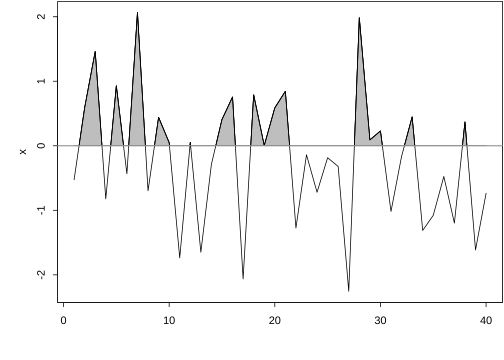
\includegraphics{elements_files/figure-latex/polygon-demo-1} 

}

\caption[多边形和矩形结合使用的一个巧妙图示]{多边形和矩形结合使用的一个巧妙图示:将 0 上下的数值分别用不同颜色填充。本图也可以利用 \texttt{clip()} 函数更方便地完成,请读者自行查阅帮助。}\label{fig:polygon-demo}
\end{figure}





最后要说明,其实还有一个特殊的``矩形'',那就是整幅图形的边框,它可以用 \texttt{box()} 函数来完成。我们可以不使用任何参数以添加默认的边框,也可以调整一些参数画出不同样式的方框(如虚线框等),具体参见 \texttt{?box}。

关于多边形和矩形,我们用一个比较巧妙的例子来说明具体用法,代码和效果参见图 \ref{fig:polygon-demo}。这幅图的目的在于只填充 y 值在 0 以上的部分,0 以下的部分留空。采取的手段是:先用多边形整体填充颜色,然后根据当前图形的坐标范围(用 \texttt{par(\textquotesingle{}usr\textquotesingle{})} 获得(或者等价使用 \texttt{par()\$usr}),参见 \ref{sec:par} 小节)画一个白色的矩形覆盖 0 以下的图形部分,此时下面部分的线条也被覆盖了,因此接着我们必须再次画线,将所有线条补充完整,最后,添加一条高度为 0 的水平线,即完成本图。

\begin{Shaded}
\begin{Highlighting}[]
\FunctionTok{demo}\NormalTok{(}\StringTok{"kaleidoscope"}\NormalTok{, }\AttributeTok{package =} \StringTok{"MSG"}\NormalTok{)}
\end{Highlighting}
\end{Shaded}

\begin{figure}

{\centering 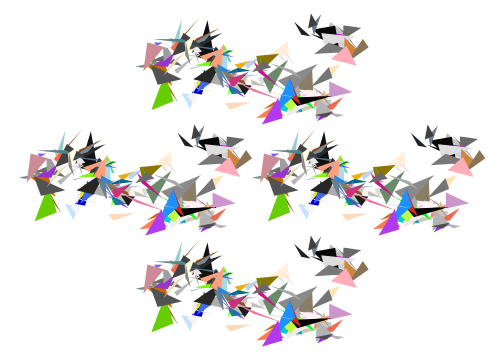
\includegraphics{elements_files/figure-latex/polygon-kaleidoscope-1} 

}

\caption[ 用多边形生成的“万花筒”]{用多边形生成的``万花筒'':若干彩色三角形(或者称之为``千纸鹤图''?)}\label{fig:polygon-kaleidoscope}
\end{figure}



图 \ref{fig:polygon-kaleidoscope} 是利用含有缺失值的数据画出来的多边形,它看起来与万花筒图案有些相似(本例为``彩蛋'')。这幅图的生成过程是:随机生成 3 个标准正态分布随机数,然后插入一个缺失值 NA,下一次再以上一批随机数的最后一个为均值生成 3 个随机数,依此类推生成若干组``三个随机数加上一个 NA''这样的数据,这样最后画多边形的时候,得到的就是若干个独立的三角形。我们将这一组三角形分别向右、向上和向下平移,得到四组三角形,也就是不太精确地模仿了万花筒的原理。该演示收录在 \textbf{MSG} 包中,读者可用 \texttt{demo(\textquotesingle{}kaleidoscope\textquotesingle{},\ package\ =\ \textquotesingle{}MSG\textquotesingle{})} 查看源代码。

\section{网格线}\label{sec:grid}

有时为了方便图形阅读者知道图中元素的更精确的位置,我们可以用添加背景网格线的办法来辅助读者的视线对齐坐标轴。函数 \texttt{grid()} 所实现的就是这一个功能,它的用法较简单:

\begin{Shaded}
\begin{Highlighting}[]
\FunctionTok{usage}\NormalTok{(grid)}
\end{Highlighting}
\end{Shaded}

\begin{verbatim}
## grid(nx = NULL, ny = nx, col = "lightgray", lty = "dotted", lwd = par("lwd"),
##   equilogs = TRUE)
\end{verbatim}

可以看到,这个函数已经使用了一些默认的参数设置,例如将网格线的颜色设置为浅灰色,线条样式设置为点线,这是一种比较美观的设置,让网格线既不显得太突兀,又能达到辅助的效果;一般情况下,我们可以直接使用不带参数的 \texttt{grid()} 函数添加网格。参数 \texttt{nx} 和 \texttt{ny} 分别表示横纵轴上网格线的条数,颜色、线条样式和线条宽度参数不必再说明,最后 \texttt{equilogs} 参数意思是,当坐标取了对数之后,是依然使用等距的网格线(\texttt{TRUE})还是根据对数函数使用不等距的网格线(\texttt{FALSE})。

细心的读者也许能发现,其实前面讲到的内容中已经有两处可以实现``网格线''的功能,第一处是 \texttt{par()} 函数中的 \texttt{tcl}(或 \texttt{tck}),将坐标轴的刻度线长度设置为图形的宽高就可以构成一种粗略的网格;第二处是 \texttt{abline()} 函数,使用参数 \texttt{h} 和 \texttt{v} 即可实现更细致的网格线。

\section{标题、任意文本、周边文本}\label{sec:text}

本节中的文本以及下一节中的图例都是用来辅助解释图形的信息,图形中的所有文本可以分为三类:标题(主副标题和坐标轴标题)、任意文本和图形周边文本。\texttt{title()} 函数用来添加标题,\texttt{text()} 函数用来向图形中任意位置添加文本,\texttt{mtext()} 函数用来向图的四条边上添加文本。用法如下:

\begin{Shaded}
\begin{Highlighting}[]
\FunctionTok{usage}\NormalTok{(title)}
\end{Highlighting}
\end{Shaded}

\begin{verbatim}
## title(main = NULL, sub = NULL, xlab = NULL, ylab = NULL, line = NA,
##   outer = FALSE, ...)
\end{verbatim}

\begin{Shaded}
\begin{Highlighting}[]
\FunctionTok{usage}\NormalTok{(text, }\StringTok{"default"}\NormalTok{)}
\end{Highlighting}
\end{Shaded}

\begin{verbatim}
## text(x, ...)
\end{verbatim}

\begin{Shaded}
\begin{Highlighting}[]
\FunctionTok{usage}\NormalTok{(mtext)}
\end{Highlighting}
\end{Shaded}

\begin{verbatim}
## mtext(text, side = 3, line = 0, outer = FALSE, at = NA, adj = NA, padj = NA,
##   cex = NA, col = NA, font = NA, ...)
\end{verbatim}

若无特别设定,这些文本的样式都将根据当前的函数 \texttt{par()} 结果来设置,比如颜色、字体等。函数 \texttt{title()} 的前四个参数就是主、副、x 轴、y 轴标题的字符串,\texttt{line} 设置一个距离图形边缘的行数(即:文本与图形边缘的距离为 line\(\times\) 行高);\texttt{outer} 表示是否将文本放在外边界中(参见 \ref{sec:par} 小节的说明);函数 \texttt{text()} 的参数 \texttt{labels} 就是欲添加的文本(对应横纵坐标的设置,可以是字符串向量),若不指定本参数,那么默认将以数字 \texttt{1:length(x)} 作为文本标记添加到图中;\texttt{adj} 与 \texttt{par()} 中说明相同;\texttt{pos} 参数取值整数 1\textasciitilde4 分别表示文本的位置在坐标点的下、左、上、右方,注意,它会覆盖参数 \texttt{adj} 的设置;\texttt{offset} 参数会根据 \texttt{pos} 参数的取值将文本向相应的方向移动一定比例的距离;\texttt{vfont} 参数用 Hershey 矢量字体来设置文本的字体式样,取值长度为 2 的向量,第一个元素指定字体(Typeface),第二个元素指定式样(Style),关于字体和式样的搭配种类,请查看帮助 \texttt{?Hershey},使用 Hershey 矢量字体的优势在于:

\begin{itemize}
\tightlist
\item
  Hershey 字体会产生更好的输出,特别在计算机屏幕上,或者用于旋转以及小字体时
\item
  Hershey 字体提供一些标准字体库没有的字体。如提供星座记号,地图符号和天文学符号
\item
  Hershey 字体提供西里尔字符(cyrillic)和日语字符(假名和日本汉字)
\end{itemize}

此外,等高线图中通常使用 Hershey 矢量字体以使等高线上的文本更清晰好看,由于字体设置搭配内容体系比较庞大,因此感兴趣的读者请仔细阅读帮助(该字体的一个缺陷是不能用在数学公式中);\texttt{side} 参数取值为整数 1\textasciitilde4 分别把周边文本作在表示图形的下、左、上、右边;其它参数基本已经都已经接触过,有些不常用的参数在此处省略不讲。

\section{图例}\label{sec:legend}

\begin{Shaded}
\begin{Highlighting}[]
\FunctionTok{par}\NormalTok{(}\AttributeTok{mar =} \FunctionTok{c}\NormalTok{(}\DecValTok{4}\NormalTok{, }\DecValTok{4}\NormalTok{, }\DecValTok{4}\NormalTok{, }\DecValTok{3}\NormalTok{))}
\FunctionTok{plot}\NormalTok{(}\DecValTok{0}\SpecialCharTok{:}\DecValTok{10}\NormalTok{, }\AttributeTok{type =} \StringTok{"n"}\NormalTok{, }\AttributeTok{xlab =} \StringTok{""}\NormalTok{, }\AttributeTok{ylab =} \StringTok{""}\NormalTok{, }\AttributeTok{xlim =} \FunctionTok{c}\NormalTok{(}\DecValTok{0}\NormalTok{, }\DecValTok{12}\NormalTok{))}
\FunctionTok{grid}\NormalTok{(}\AttributeTok{col =} \StringTok{"gray"}\NormalTok{)}
\FunctionTok{title}\NormalTok{(}
  \AttributeTok{main =} \StringTok{"Demonstration of text in R Graphics"}\NormalTok{,}
  \AttributeTok{xlab =} \StringTok{"X{-}axis title"}\NormalTok{, }\AttributeTok{ylab =} \StringTok{"Y{-}axis title"}
\NormalTok{)}
\FunctionTok{mtext}\NormalTok{(}\StringTok{"Here is }\SpecialCharTok{\textbackslash{}"}\StringTok{side = 4}\SpecialCharTok{\textbackslash{}"}\StringTok{"}\NormalTok{, }\AttributeTok{side =} \DecValTok{4}\NormalTok{, }\AttributeTok{line =} \DecValTok{1}\NormalTok{)}
\NormalTok{x }\OtherTok{\textless{}{-}} \FunctionTok{c}\NormalTok{(}\DecValTok{6}\NormalTok{, }\DecValTok{4}\NormalTok{, }\DecValTok{6}\NormalTok{, }\DecValTok{8}\NormalTok{)}
\NormalTok{y }\OtherTok{\textless{}{-}} \FunctionTok{c}\NormalTok{(}\DecValTok{8}\NormalTok{, }\DecValTok{5}\NormalTok{, }\DecValTok{2}\NormalTok{, }\DecValTok{5}\NormalTok{)}
\NormalTok{s }\OtherTok{\textless{}{-}} \FunctionTok{c}\NormalTok{(}\DecValTok{0}\NormalTok{, }\DecValTok{90}\NormalTok{, }\DecValTok{180}\NormalTok{, }\DecValTok{270}\NormalTok{)}
\ControlFlowTok{for}\NormalTok{ (i }\ControlFlowTok{in} \DecValTok{1}\SpecialCharTok{:}\DecValTok{4}\NormalTok{) \{}
  \FunctionTok{text}\NormalTok{(x[i], y[i], }\FunctionTok{sprintf}\NormalTok{(}\StringTok{"srt = \%d"}\NormalTok{, s[i]), }\AttributeTok{srt =}\NormalTok{ s[i])}
\NormalTok{\}}
\FunctionTok{segments}\NormalTok{(}\FunctionTok{c}\NormalTok{(}\DecValTok{6}\NormalTok{, }\DecValTok{0}\NormalTok{, }\DecValTok{6}\NormalTok{, }\DecValTok{12}\NormalTok{), }\FunctionTok{c}\NormalTok{(}\DecValTok{10}\NormalTok{, }\DecValTok{5}\NormalTok{, }\DecValTok{0}\NormalTok{, }\DecValTok{5}\NormalTok{), }\FunctionTok{c}\NormalTok{(}\DecValTok{0}\NormalTok{, }\DecValTok{6}\NormalTok{, }\DecValTok{12}\NormalTok{, }\DecValTok{6}\NormalTok{),}
  \FunctionTok{c}\NormalTok{(}\DecValTok{5}\NormalTok{, }\DecValTok{0}\NormalTok{, }\DecValTok{5}\NormalTok{, }\DecValTok{10}\NormalTok{),}
  \AttributeTok{lty =} \FunctionTok{c}\NormalTok{(}\DecValTok{2}\NormalTok{, }\DecValTok{1}\NormalTok{, }\DecValTok{1}\NormalTok{, }\DecValTok{2}\NormalTok{)}
\NormalTok{)}
\FunctionTok{legend}\NormalTok{(}\SpecialCharTok{{-}}\FloatTok{0.2}\NormalTok{, }\FloatTok{9.8}\NormalTok{, }\FunctionTok{c}\NormalTok{(}\StringTok{"Upper"}\NormalTok{, }\StringTok{"Lower"}\NormalTok{),}
  \AttributeTok{lty =} \DecValTok{2}\SpecialCharTok{:}\DecValTok{1}\NormalTok{, }\AttributeTok{cex =} \FloatTok{0.8}\NormalTok{,}
  \AttributeTok{bty =} \StringTok{"n"}
\NormalTok{)}
\end{Highlighting}
\end{Shaded}

\begin{figure}

{\centering 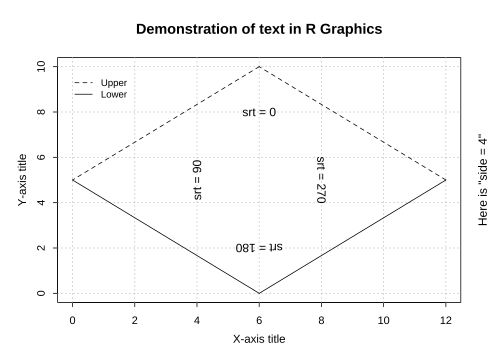
\includegraphics{elements_files/figure-latex/text-1} 

}

\caption{添加标题、任意文本和周边文本的一个演示}\label{fig:text}
\end{figure}

函数 \texttt{legend()} 的作用是添加图例,总所周知,图例也是很重要的辅助信息,告诉图形使用者图中各组不同样式的元素分别代表何种对象。它的参数比较多,但实际应用中通常仅仅用到其中少数几个:

\begin{Shaded}
\begin{Highlighting}[]
\FunctionTok{usage}\NormalTok{(legend)}
\end{Highlighting}
\end{Shaded}

\begin{verbatim}
## legend(x, y = NULL, legend, fill = NULL, col = par("col"), border = "black",
##   lty, lwd, pch, angle = 45, density = NULL, bty = "o", bg = par("bg"),
##   box.lwd = par("lwd"), box.lty = par("lty"), box.col = par("fg"), pt.bg = NA,
##   cex = 1, pt.cex = cex, pt.lwd = lwd, xjust = 0, yjust = 1, x.intersp = 1,
##   y.intersp = 1, adj = c(0, 0.5), text.width = NULL, text.col = par("col"),
##   text.font = NULL, merge = do.lines && has.pch, trace = FALSE, plot = TRUE,
##   ncol = 1, horiz = FALSE, title = NULL, inset = 0, xpd,
##   title.col = text.col[1], title.adj = 0.5, title.cex = cex[1],
##   title.font = text.font[1], seg.len = 2)
\end{verbatim}

前两个参数 \texttt{x} 和 \texttt{y} 表示图例的坐标位置(左上角顶点的坐标);\texttt{legend} 参数通常为一个字符向量,表示图例中的文字;\texttt{fill} 参数指定一个与图例字符向量对应的颜色向量用以在文本左边绘制一个颜色填充方块;\texttt{col} 参数设置图例中点和线的颜色;\texttt{lty}、\texttt{lwd} 和 \texttt{pch} 参数指定图例中点线的样式;\texttt{angle} 和 \texttt{density} 参数效果类似于 \texttt{fill} 参数,只是换成指定角度和密度的阴影线填充方块;\texttt{bty} 参数设置图例框的样式,很类似 \texttt{par()} 中的同名参数;\texttt{title} 参数设定图例的标题;剩余参数用来设置更细微的地方,不太常用。

从以上几节对图形元素的介绍可以看出,R 可以设置极其细微的元素特征,当然,读者不必过于细究所有的参数,对于大多数函数来说,都只有两三个核心参数,比如,坐标位置向量是几乎所有函数的共同核心参数,而 \texttt{legend()} 函数的主要参数除此之外还有字符向量 \texttt{legend}。对于其它参数,请在使用时即时查阅即可。

关于网格线、文本和图例,图 \ref{fig:text} 给出了它们的示例。

\section{坐标轴}\label{sec:axis}

坐标轴是图中元素所代表数值大小的参照物,因此它在图形中的作用也很重要,特别是有时候我们需要对坐标轴做一定的特殊设置,比如作一幅双坐标轴的图形,或者在坐标轴标记中使用特殊的文本,那么就必须使用 \texttt{axis()} 函数来辅助完成对坐标轴的设置和调整。该函数的用法如下:

\begin{Shaded}
\begin{Highlighting}[]
\FunctionTok{usage}\NormalTok{(axis)}
\end{Highlighting}
\end{Shaded}

\begin{verbatim}
## axis(side, at = NULL, labels = TRUE, tick = TRUE, line = NA, pos = NA,
##   outer = FALSE, font = NA, lty = "solid", lwd = 1, lwd.ticks = lwd,
##   col = NULL, col.ticks = NULL, hadj = NA, padj = NA, gap.axis = NA, ...)
\end{verbatim}

\begin{Shaded}
\begin{Highlighting}[]
\FunctionTok{data}\NormalTok{(Export.USCN, }\AttributeTok{package =} \StringTok{"MSG"}\NormalTok{)}
\FunctionTok{par}\NormalTok{(}\AttributeTok{mar =} \FunctionTok{c}\NormalTok{(}\DecValTok{4}\NormalTok{, }\FloatTok{4.5}\NormalTok{, .}\DecValTok{1}\NormalTok{, }\FloatTok{4.5}\NormalTok{))}
\CommentTok{\# 看似条形图,实为粗线条,宽度 lwd = 10}
\FunctionTok{plot}\NormalTok{(}\DecValTok{1}\SpecialCharTok{:}\DecValTok{13}\NormalTok{, Export.USCN}\SpecialCharTok{$}\NormalTok{Export,}
  \AttributeTok{xlab =} \StringTok{"Year / Country"}\NormalTok{,}
  \AttributeTok{ylab =} \StringTok{"US Dollars ($10\^{}\{16\}$)"}\NormalTok{, }\AttributeTok{xaxt =} \StringTok{"n"}\NormalTok{, }\AttributeTok{type =} \StringTok{"h"}\NormalTok{,}
  \AttributeTok{lwd =} \DecValTok{10}\NormalTok{, }\AttributeTok{col =} \FunctionTok{c}\NormalTok{(}\FunctionTok{rep}\NormalTok{(}\DecValTok{2}\NormalTok{, }\DecValTok{6}\NormalTok{), }\ConstantTok{NA}\NormalTok{, }\FunctionTok{rep}\NormalTok{(}\DecValTok{4}\NormalTok{, }\DecValTok{6}\NormalTok{)), }\AttributeTok{lend =} \DecValTok{1}\NormalTok{,}
  \AttributeTok{panel.first =} \FunctionTok{grid}\NormalTok{()}
\NormalTok{)}
\CommentTok{\# 设置 x 轴的刻度标记:\textbackslash{}n 的意思是换行符}
\NormalTok{xlabel }\OtherTok{\textless{}{-}} \FunctionTok{paste}\NormalTok{(Export.USCN}\SpecialCharTok{$}\NormalTok{Year, }\StringTok{"}\SpecialCharTok{\textbackslash{}n}\StringTok{"}\NormalTok{, Export.USCN}\SpecialCharTok{$}\NormalTok{Country)}
\NormalTok{xlabel[}\DecValTok{7}\NormalTok{] }\OtherTok{\textless{}{-}} \StringTok{""}
\FunctionTok{abline}\NormalTok{(}\AttributeTok{v =} \DecValTok{7}\NormalTok{, }\AttributeTok{lty =} \DecValTok{2}\NormalTok{) }\CommentTok{\# 添加一条分隔线}
\CommentTok{\# 使用带有换行符的刻度标记}
\FunctionTok{axis}\NormalTok{(}\DecValTok{1}\NormalTok{, }\DecValTok{1}\SpecialCharTok{:}\DecValTok{13}\NormalTok{, }\AttributeTok{labels =}\NormalTok{ xlabel, }\AttributeTok{tick =} \ConstantTok{FALSE}\NormalTok{, }\AttributeTok{cex.axis =} \FloatTok{0.75}\NormalTok{)}
\CommentTok{\# 换算为人民币再计算另一个坐标轴刻度(汇率 8.27)}
\NormalTok{ylabel }\OtherTok{\textless{}{-}} \FunctionTok{pretty}\NormalTok{(Export.USCN}\SpecialCharTok{$}\NormalTok{Export }\SpecialCharTok{*} \FloatTok{8.27}\NormalTok{)}
\FunctionTok{axis}\NormalTok{(}\DecValTok{4}\NormalTok{, }\AttributeTok{at =}\NormalTok{ ylabel }\SpecialCharTok{/} \FloatTok{8.27}\NormalTok{, }\AttributeTok{labels =}\NormalTok{ ylabel)}
\FunctionTok{mtext}\NormalTok{(}\StringTok{"Chinese RMB ($10\^{}\{16\}$)"}\NormalTok{, }\AttributeTok{side =} \DecValTok{4}\NormalTok{, }\AttributeTok{line =} \DecValTok{2}\NormalTok{)}
\FunctionTok{box}\NormalTok{()}
\end{Highlighting}
\end{Shaded}

\begin{figure}

{\centering 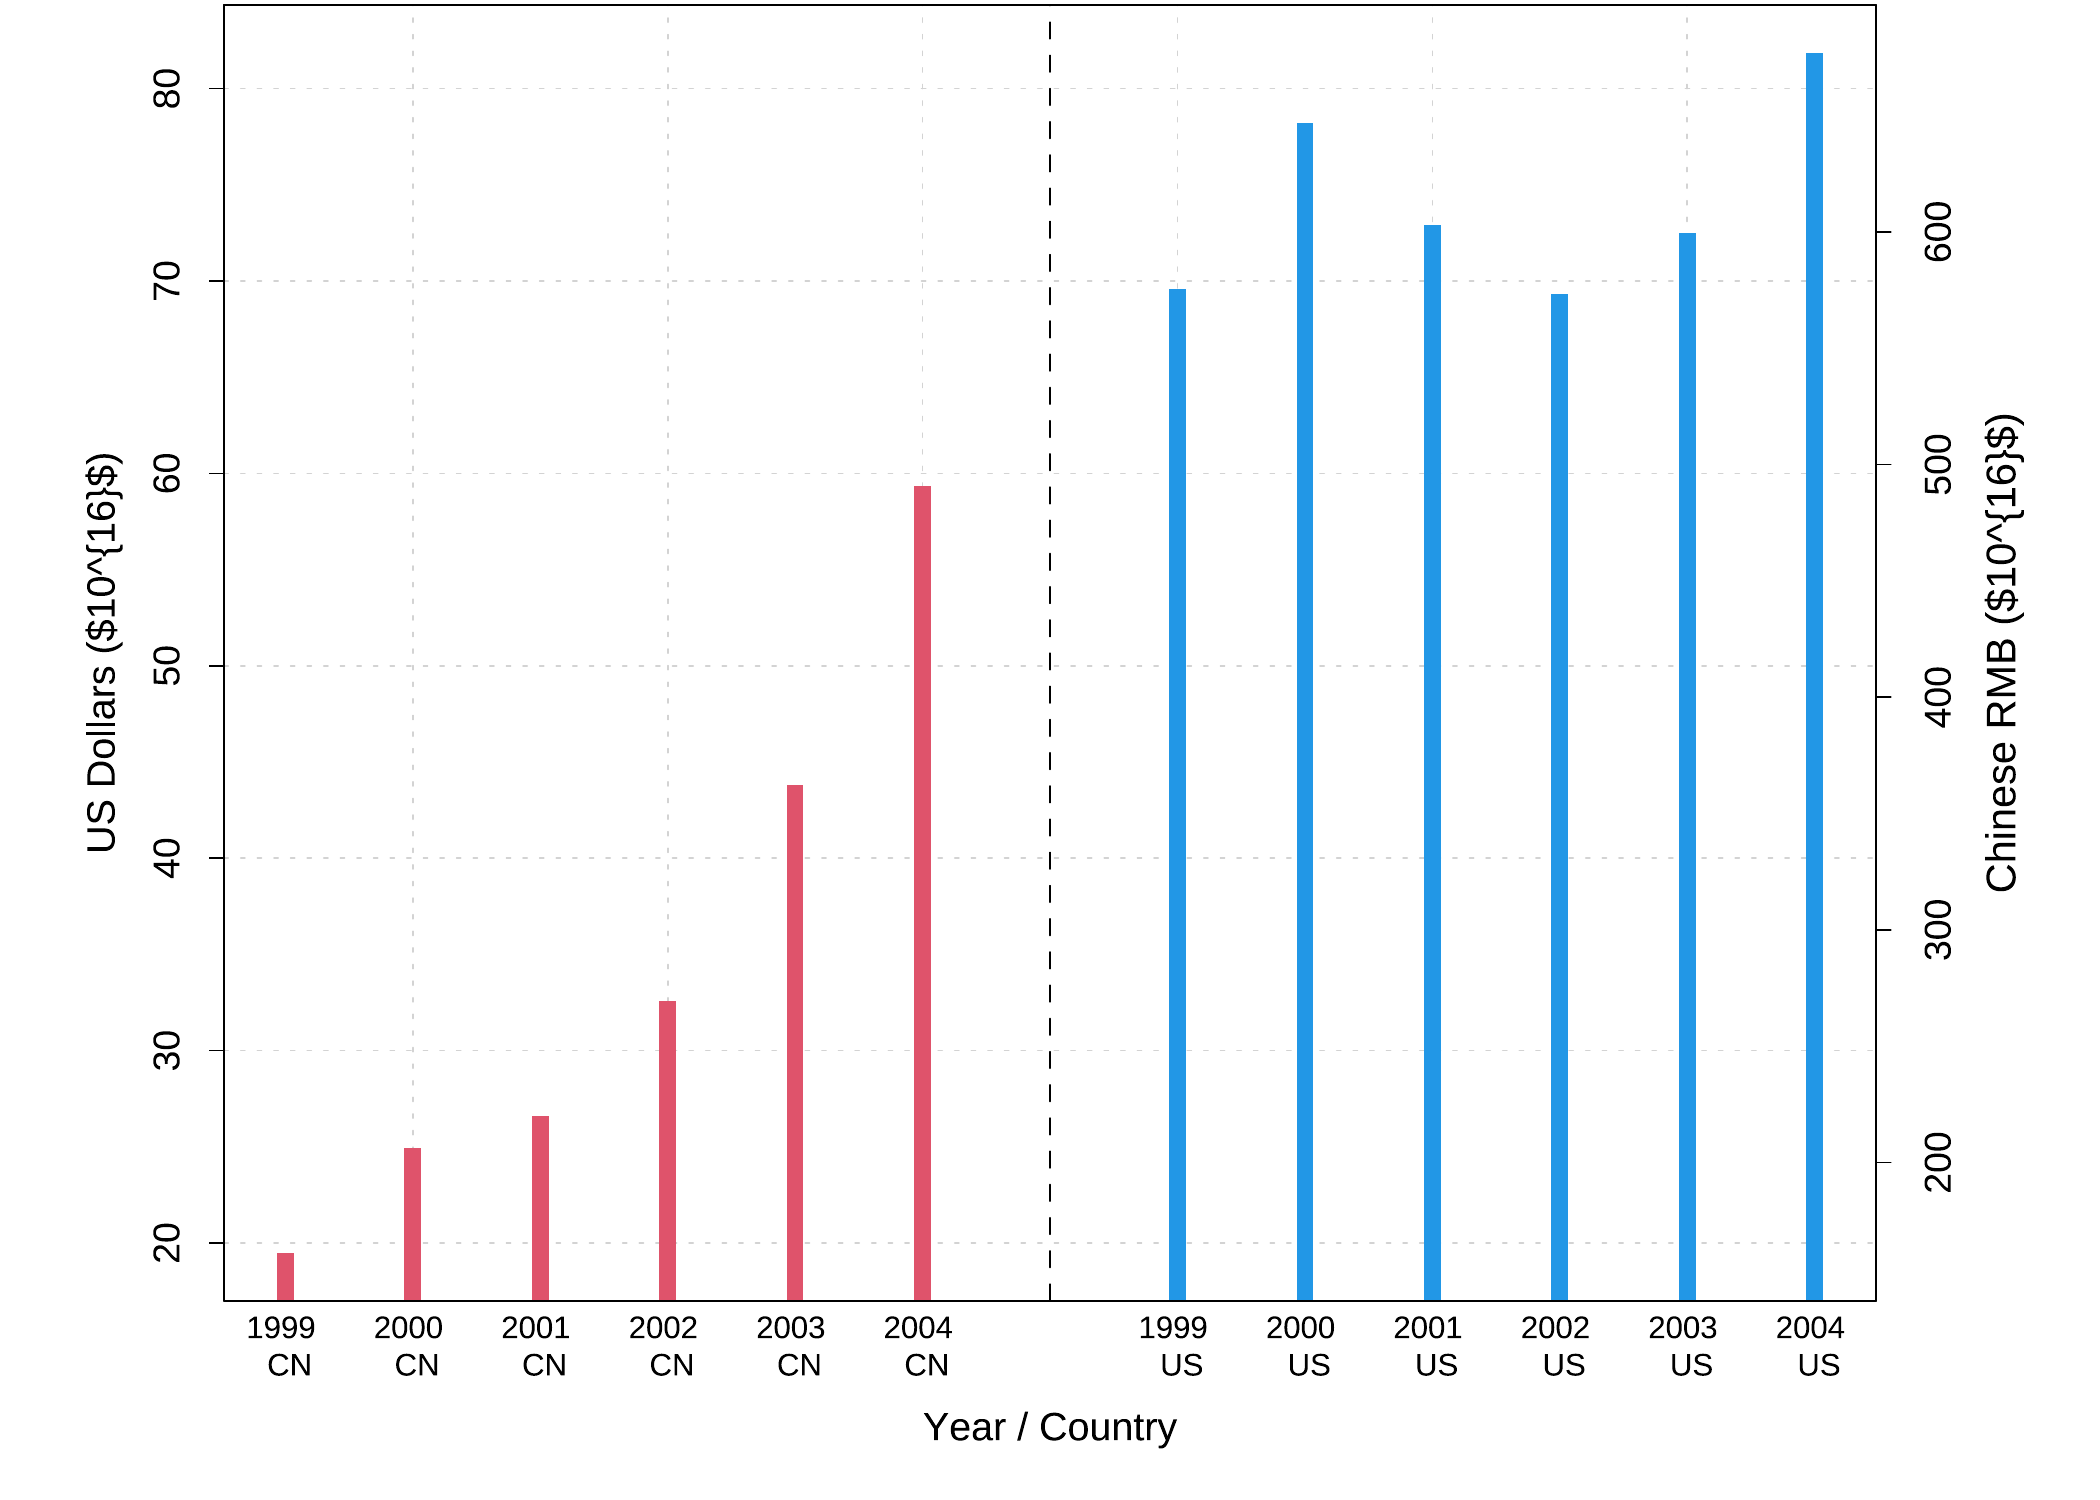
\includegraphics{elements_files/figure-latex/axis-demo-1} 

}

\caption[中美出口额双坐标轴图示]{双坐标轴图示:中美两国 1999\textasciitilde2004 年出口额,分别以美元和人民币表示。注意图中 x 轴标签文本是如何换行的。}\label{fig:axis-demo}
\end{figure}



其中,\texttt{side} 参数与 \texttt{mtext()} 函数中的参数意思相类似,表示将坐标轴画在哪条边上,事实上通过前面一些图形元素参数的讲解,读者应该能意识到,R 中上下左右方向的顺序一般都是``下、左、上、右'',分别用 1、2、3、4 表示;\texttt{at} 参数表示在什么位置画坐标轴标记线;\texttt{labels} 参数指定坐标轴刻度标记的字符。

\citet{Murrell05} 中第 3.4.5 小节举了一个双坐标轴图形的例子,图中用左右两边的纵轴分别表示摄氏和华氏的温度,即:对于图中同一点,既可以对照左边看摄氏度,也可以对照右边看华氏度;这就是双坐标轴的用途。此处我们不妨也举一个类似的例子来说明 \texttt{axis()} 函数的功能。图 \ref{fig:axis-demo} 展示的是从 1999\textasciitilde2004 年中美两国的出口贸易总额,其中 \texttt{axis()} 函数主要作用在于两个地方:第一点是横轴的刻度标记,注意这些刻度标记与我们平时看到的标记有所不同,主要是这一系列标记都是两行文本,原因就在于 \texttt{labels} 参数中使用了换行符,对 C 语言比较熟悉的读者对此不会感到陌生,这里第一行是年份,第二行说明了国家:CN 表示中国,US 表示美国;第二点是图的右边多了一根坐标轴,左边的纵轴表示出口额按美元计价(单位:\(10^{16}\) 美元,出口额数值太大,因此采用较大的单位),右边表示同样的出口额用人民币计价(例如右边轴上 400 人民币对应左边 \(400/8.27\approx48.4\) 美元),同一个数值在图中既可以从左边观察美元金额,又可以从右边观察人民币金额。本例中使用的数据来源为:汇率数据来自联合国统计署网站 \url{https://unstats.un.org},从 1999\textasciitilde2004 年人民币和美元的平均汇率稳定在 8.27,出口额年度数据来自 WTO 网站:\url{https://data.wto.org}。整理后的数据如下,程序代码可以参见图 \ref{fig:axis-demo}。

\begin{Shaded}
\begin{Highlighting}[]
\FunctionTok{data}\NormalTok{(Export.USCN, }\AttributeTok{package =} \StringTok{"MSG"}\NormalTok{)}
\NormalTok{Export.USCN}
\end{Highlighting}
\end{Shaded}

\begin{verbatim}
##     Export Year Country
## 1  19.4931 1999      CN
## 2  24.9203 2000      CN
## 3  26.6098 2001      CN
## 4  32.5596 2002      CN
## 5  43.8228 2003      CN
## 6  59.3326 2004      CN
## 7       NA   NA    <NA>
## 8  69.5797 1999      US
## 9  78.1918 2000      US
## 10 72.9100 2001      US
## 11 69.3103 2002      US
## 12 72.4771 2003      US
## 13 81.8520 2004      US
\end{verbatim}

\section{图形元素应用示例}\label{ux56feux5f62ux5143ux7d20ux5e94ux7528ux793aux4f8b}

在介绍了图形的基本构成元素的作法之后,我们应该可以理解 R 作图的自由------几乎所有图形的细节都可以被我们控制。下面我们举几个例子来说明如何利用图形元素来构造完整的图形。

\subsection{瀑布图}\label{subsec:waterfall-chart}

瀑布图(Waterfall Chart)的最初发明者我们无法考证,但可以在麦肯锡的报告中看到它的身影。如果在 Google 中搜索 Excel 瀑布图,我们可以看见一些令人无奈的结果,例如

\begin{quote}
步步致赢瀑布图(步行图)制作系统 1.1 {[}\ldots{]} 下载 {[}\ldots{]} 共享版最多支持 6 个数,正式版无限制。
\end{quote}

或是

\begin{quote}
瀑布图的完美解决方案 {[}Excel 图表{]} {[}\ldots{]} 简单说明一下:{[}\ldots{]} (分为 6 步)
\end{quote}

作者曾在某咨询公司听过一场关于 Excel 作图的培训,其中也大谈瀑布图的技巧,大致思路是用一些本来不直观的方法来完成瀑布图的制作,例如用白色填充矩形条,使之``隐藏''起来,而上面的矩形条才能得到``悬空''的效果。

瀑布图究竟是什么呢?只不过是一系列矩形而已(\ref{sec:polygon} 小节)。它的外观类似于条形图,区别在于除了第一个矩形条之外,后面的矩形条都不再以零点为基准线来画,而是以前一个矩形条的高度为起点画矩形到该矩形条位置上的取值,这样可以反映一个变量取值的上下变化情况(主要是体现相邻矩形条的差值)。下面我们结合一个数据实例来说明瀑布图的简单思想和简单做法。

我们选取了 2010 年 8 月第一周``统计之都''网站的``绝对唯一访问次数''(Absolute Unique Visitors)来画瀑布图,数据如下

\begin{Shaded}
\begin{Highlighting}[]
\CommentTok{\# 七天之内的唯一访问次数数据(周一为 2010 年 8 月 2 日)}
\NormalTok{auv }\OtherTok{\textless{}{-}} \FunctionTok{c}\NormalTok{(}\DecValTok{939}\NormalTok{, }\DecValTok{1005}\NormalTok{, }\DecValTok{973}\NormalTok{, }\DecValTok{910}\NormalTok{, }\DecValTok{875}\NormalTok{, }\DecValTok{658}\NormalTok{, }\DecValTok{688}\NormalTok{)}
\CommentTok{\# 相邻两天作差}
\FunctionTok{diff}\NormalTok{(auv)}
\end{Highlighting}
\end{Shaded}

\begin{verbatim}
## [1]   66  -32  -63  -35 -217   30
\end{verbatim}

瀑布图中第一个矩形条高度为 939,第二个矩形则从 939 继续向上画 \(1005-939=66\) 单位,第三个矩形则从 1005 开始向下画 32 单位,依此类推。对于访问量下滑的那些日期,可以用特殊颜色标示(比如红色警告),以区分访问量增长的日期。图 \ref{fig:waterfall-chart} 给出了 R 代码和瀑布图结果,其中核心代码只有最后一句,前面的代码仅以布局和美观为目的。从代码可以看到,我们用低层作图函数 \texttt{rect()} 来画瀑布图是非常直观的:前四个参数给定了矩形的位置坐标,而这些位置经过简单的逻辑思考很容易得到。所有任务只是画矩形而已,在缺少对图形元素充分支持的软件包中,我们付出了不必要的代价。

\begin{Shaded}
\begin{Highlighting}[]
\FunctionTok{par}\NormalTok{(}\AttributeTok{mar =} \FunctionTok{c}\NormalTok{(}\DecValTok{4}\NormalTok{, }\DecValTok{4}\NormalTok{, .}\DecValTok{5}\NormalTok{, .}\DecValTok{1}\NormalTok{))}
\FunctionTok{plot}\NormalTok{(auv,}
  \AttributeTok{xlab =} \StringTok{"八月第一周"}\NormalTok{,}
  \AttributeTok{ylab =} \StringTok{"绝对唯一访问次数"}\NormalTok{, }\AttributeTok{type =} \StringTok{"n"}\NormalTok{,}
  \AttributeTok{xlim =} \FunctionTok{c}\NormalTok{(}\FloatTok{0.5}\NormalTok{, }\FloatTok{7.5}\NormalTok{),}
  \AttributeTok{ylim =} \FunctionTok{c}\NormalTok{(}\DecValTok{0}\NormalTok{, }\FunctionTok{max}\NormalTok{(auv)),}
  \AttributeTok{xaxt =} \StringTok{"n"}\NormalTok{, }\AttributeTok{panel.first =} \FunctionTok{grid}\NormalTok{()}
\NormalTok{)}
\FunctionTok{axis}\NormalTok{(}\DecValTok{1}\NormalTok{, }\DecValTok{1}\SpecialCharTok{:}\DecValTok{7}\NormalTok{, }\FunctionTok{sprintf}\NormalTok{(}\StringTok{"周\%s"}\NormalTok{, }\FunctionTok{c}\NormalTok{(}
  \StringTok{"一"}\NormalTok{, }\StringTok{"二"}\NormalTok{, }\StringTok{"三"}\NormalTok{, }\StringTok{"四"}\NormalTok{, }\StringTok{"五"}\NormalTok{, }\StringTok{"六"}\NormalTok{, }\StringTok{"日"}
\NormalTok{)))}
\FunctionTok{rect}\NormalTok{(}\DecValTok{1}\SpecialCharTok{:}\DecValTok{7} \SpecialCharTok{{-}} \FloatTok{0.3}\NormalTok{, }\FunctionTok{c}\NormalTok{(}\DecValTok{0}\NormalTok{, auv[}\DecValTok{1}\SpecialCharTok{:}\DecValTok{6}\NormalTok{]), }\DecValTok{1}\SpecialCharTok{:}\DecValTok{7} \SpecialCharTok{+} \FloatTok{0.3}\NormalTok{, auv,}
  \AttributeTok{col =} \FunctionTok{c}\NormalTok{(}\ConstantTok{NA}\NormalTok{, }\FunctionTok{ifelse}\NormalTok{(}\FunctionTok{diff}\NormalTok{(auv) }\SpecialCharTok{\textless{}} \DecValTok{0}\NormalTok{, }\StringTok{"red"}\NormalTok{, }\ConstantTok{NA}\NormalTok{))}
\NormalTok{)}
\end{Highlighting}
\end{Shaded}

\begin{figure}

{\centering 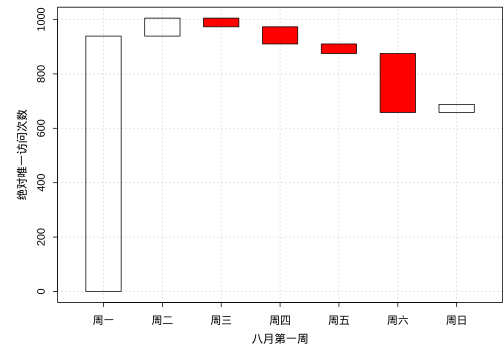
\includegraphics{elements_files/figure-latex/waterfall-chart-1} 

}

\caption[``统计之都''网站八月第一周访问数据瀑布图]{``统计之都''网站八月第一周访问数据瀑布图:周一访问量为 939, 周二上升,周三开始下降(红色矩形表示访问量下降),直到周末降到最低。这个规律在其它星期都存在,也许它反映了大众普遍的劳累和忙碌规律?}\label{fig:waterfall-chart}
\end{figure}





\subsection{梯度下降算法}\label{subsec:grad-desc}

箭头在图形中的作用通常是指示,例如图 \ref{fig:lines-demo} 中的箭头用来将文本标注指向一条直线,这样使得文本的位置可以灵活安排。下面我们再给一个看起来更复杂的例子,来说明箭头的一个自然而然应用。很多统计计算过程都涉及到迭代,因为这些计算问题没有显式解(即:没有明确的数学表达式),很难一步得到答案,但可以通过迭代来一步步逼近真实解,梯度下降算法就是诸多具有迭代特征方法中的一种。梯度下降算法的目标在于寻找一个函数 \(F(\mathsf{x})\) 的极值,不失一般性,我们假设寻找的是极小值。这里我们简单描述一些梯度下降算法的原理:

假设函数 \(F(\mathsf{x})\) 在点 \(\mathsf{a}\) 的一个小邻域内可导(这里 \(\mathsf{x}\) 可以是多维向量),那么从点 \(\mathsf{a}\) 出发,\(F(\mathsf{x})\) 沿负梯度方向 \(-\nabla F(\mathsf{a})\) 函数值下降最快。可以证明对足够小的 \(\gamma>0\),若

\[\mathsf{b} = \mathsf{a}-\gamma\nabla F(\mathsf{a})\]
那么 \(F(\mathsf{a})\geq F(\mathsf{b})\)。这样,我们随机猜测一个迭代的起点 \(\mathsf{x}_{0}\),然后按以下方式迭代计算下一步的解 \(\mathsf{x}_{n}\):

\[\mathsf{x}_{n+1} = \mathsf{x}_{n}-\gamma\nabla F(\mathsf{x}_{n}),\ n\ge0\]

即可满足:

\[F(\mathsf{x}_{0})\ge F(\mathsf{x}_{1})\ge F(\mathsf{x}_{2})\ge\cdots\]

这样序列 \(\left\{ \mathsf{x}_{n}\right\}\) 将收敛到局部最小值。

上述算法中,核心计算就是目标函数 F 的导数(多维情况下通常称为梯度),剩下的就是简单的四则运算。求导可以用 R 自身的函数 \texttt{deriv()},所以这个计算实现起来并不困难,而我们想要通过一个例子来说明几个在统计计算中容易被广大统计应用者忽略的问题:

\begin{enumerate}
\def\labelenumi{\arabic{enumi}.}
\tightlist
\item
  迭代的起点
\item
  步长(本算法中可以看作是 \(\gamma\))
\item
  迭代次数
\item
  误差
\end{enumerate}

我们在实际应用中,往往过于依赖和相信计算机程序,认为所有默认设置都是最优或最可靠的,实际并非如此,否则所有的函数都没有必要设置参数了。以上四个问题是大多数迭代性质的算法都会涉及到的:迭代起点通常需要和真实的解相隔较近,但这个要求不具备可操作性,因为我们并不知道真实解在哪里;步长通常尽量小,保证迭代能稳定收敛,否则迭代过程中跳跃很大不容易找到解,但小步长的缺点也很明显,它使得迭代进行得很慢;迭代次数通常需要尽量大;误差显然应该越小越好,例如在求根的问题中,我们希望目标函数值越接近于 0 越好。图 \ref{fig:gradArrows} 选取了一个二元函数

\[f(x,y)=\sin(x^{2}/2-y^{2}/4+3)\cos(2x+1-\exp(y)),\]

目标是在 \(\left\{ (x,y)|x\in[-1,1],\ y\in[0.5,2.2]\right\}\) 范围内求得一对 \((x,y)\) 使得 \(f(\cdot,\cdot)\) 最小,整幅图的背景是一幅颜色图(\ref{sec:image} 小节将会介绍),图中横轴表示 x,纵轴表示 y,每一对 \((x,y)\) 对应的地方有一个颜色方块,它的颜色深浅代表了函数 \(f(x,y)\) 的取值大小,越深表示值越小。理想情况是,我们随意选取一个迭代起点,梯度下降算法能把我们带到图中的最深处去,这个过程在图中用一系列首尾相接的箭头表示,但图 \ref{fig:gradArrows} 显示的情况并不完全与我们的预期相符:有些起始点能把我们带到低处,有些则不能;有些步长下收敛较稳定,有些步长则让迭代路径蜿蜒崎岖;有的箭头还没到最低点就停滞不前了,有些则一直能往最低的地方走。本例的目标函数也可以用 R 自身的 \texttt{optim()} 函数来求极小值,它的收敛代码为 0,表示这个计算结果在一定条件下可以收敛(但不代表找到了全局最小值,甚至不代表找到了局部最小值):

\begin{Shaded}
\begin{Highlighting}[]
\NormalTok{f2 }\OtherTok{\textless{}{-}} \ControlFlowTok{function}\NormalTok{(x) }\FunctionTok{sin}\NormalTok{(}\DecValTok{1} \SpecialCharTok{/} \DecValTok{2} \SpecialCharTok{*}\NormalTok{ x[}\DecValTok{1}\NormalTok{]}\SpecialCharTok{\^{}}\DecValTok{2} \SpecialCharTok{{-}} \DecValTok{1} \SpecialCharTok{/} \DecValTok{4} \SpecialCharTok{*}\NormalTok{ x[}\DecValTok{2}\NormalTok{]}\SpecialCharTok{\^{}}\DecValTok{2} \SpecialCharTok{+} \DecValTok{3}\NormalTok{) }\SpecialCharTok{*}
    \FunctionTok{cos}\NormalTok{(}\DecValTok{2} \SpecialCharTok{*}\NormalTok{ x[}\DecValTok{1}\NormalTok{] }\SpecialCharTok{+} \DecValTok{1} \SpecialCharTok{{-}} \FunctionTok{exp}\NormalTok{(x[}\DecValTok{2}\NormalTok{]))}
\CommentTok{\# par 为局部解;value 为目标函数值; convergence 为收敛指示代码}
\FunctionTok{optim}\NormalTok{(}\FunctionTok{c}\NormalTok{(}\SpecialCharTok{{-}}\NormalTok{.}\DecValTok{9}\NormalTok{, .}\DecValTok{9}\NormalTok{), f2, }\AttributeTok{method =} \StringTok{"L{-}BFGS{-}B"}\NormalTok{, }\AttributeTok{lower =} \FunctionTok{c}\NormalTok{(}\SpecialCharTok{{-}}\DecValTok{1}\NormalTok{, .}\DecValTok{5}\NormalTok{), }\AttributeTok{upper =} \FunctionTok{c}\NormalTok{(}\DecValTok{1}\NormalTok{, }\FloatTok{2.2}\NormalTok{))}
\end{Highlighting}
\end{Shaded}

\begin{verbatim}
## $par
## [1] 0.3227365 1.6024052
## 
## $value
## [1] -0.6574
## 
## $counts
## function gradient 
##       13       13 
## 
## $convergence
## [1] 0
## 
## $message
## [1] "CONVERGENCE: REL_REDUCTION_OF_F <= FACTR*EPSMCH"
\end{verbatim}

为了叙述方便,我们将图中最高的点编号为 1,其它点按逆时针方向依次编号。点 1 初始位置在``山脊''上,最初几步迭代可能使它到达了一个``陡峭''的区域(即导数值很大),所以在某一步迭代中一下跳到图的下方,然后不知所终;点 3 的步长大,也有跳跃性,但迂回几次之后最终还是步入了``正轨'';点 6 表现很好,但由于迭代次数很少,因此停在了在离最低点很远的地方;左下角的点 7 到点 15 都表现较好,只是有些点的迭代次数不够,停在了半路;右下角那个点迭代了几步就超出了搜索范围,可能前往另一个局部最小值去了;最后两个点由于已经足够靠近最低点,所以步长显得太大,迭代过程左右大幅摇晃,但前进方向是对的。图中每一个箭头所指的方向都是当前位置上的负梯度方向,理论上它与等高线是垂直的(本图没有加等高线,读者凭眼睛从颜色区域中简单勾勒),显然,负梯度方向大致说来都是使得函数值下降最快的方向,因为大多数箭头都是尽快往颜色最深的地方走,这使得``梯度''的含义非常直观;另外,20 个点的表现告诉我们,有些数值计算方法在特定条件下可能并不会收敛到极大值或极小值。作者对流行的结构方程模型一直持保守态度,原因就是很少有人关心计算层面的东西,把一切都交给计算机去做,殊不知结构方程模型的目标函数是何等的复杂:一个普通的模型可能就包含三十个参数,这些参数是矩阵的构成元素,而目标函数又是由矩阵的逆、行列式等运算构成。也许作者在这个问题上多虑了,但作者所看到的模型应用者几乎无人关心迭代起始点和迭代次数,甚至有人为了防止``坏情况''发生,故意将迭代初始值或者随机数种子固定住,这样的运算毫无疑问是稳定的,但它是否可靠,还值得验证。

图 \ref{fig:gradArrows} 同时展示了梯度下降算法的原理以及在应用中可能出现的问题(演示 \texttt{demo(\textquotesingle{}gradArrows2\textquotesingle{},\ package\ =\ \textquotesingle{}MSG\textquotesingle{})} 可以获得更好的图形质量以及箭头动画效果),它充分显示了 R 语言的统计图形能力可以紧密结合它的统计计算优势,创造出有意义的统计图形。我们使用的只是简单的图形元素(箭头)和基本的计算(求导),但结果的深刻远大于过程的简单。从某种程度上来说,在 R 语言中作图缺的不是工具(工具俯拾皆是),而是创意、思考以及对数据的理解。

\begin{Shaded}
\begin{Highlighting}[]
\FunctionTok{demo}\NormalTok{(}\StringTok{"gradArrows1"}\NormalTok{, }\AttributeTok{package =} \StringTok{"MSG"}\NormalTok{)}
\end{Highlighting}
\end{Shaded}

\begin{figure}

{\centering 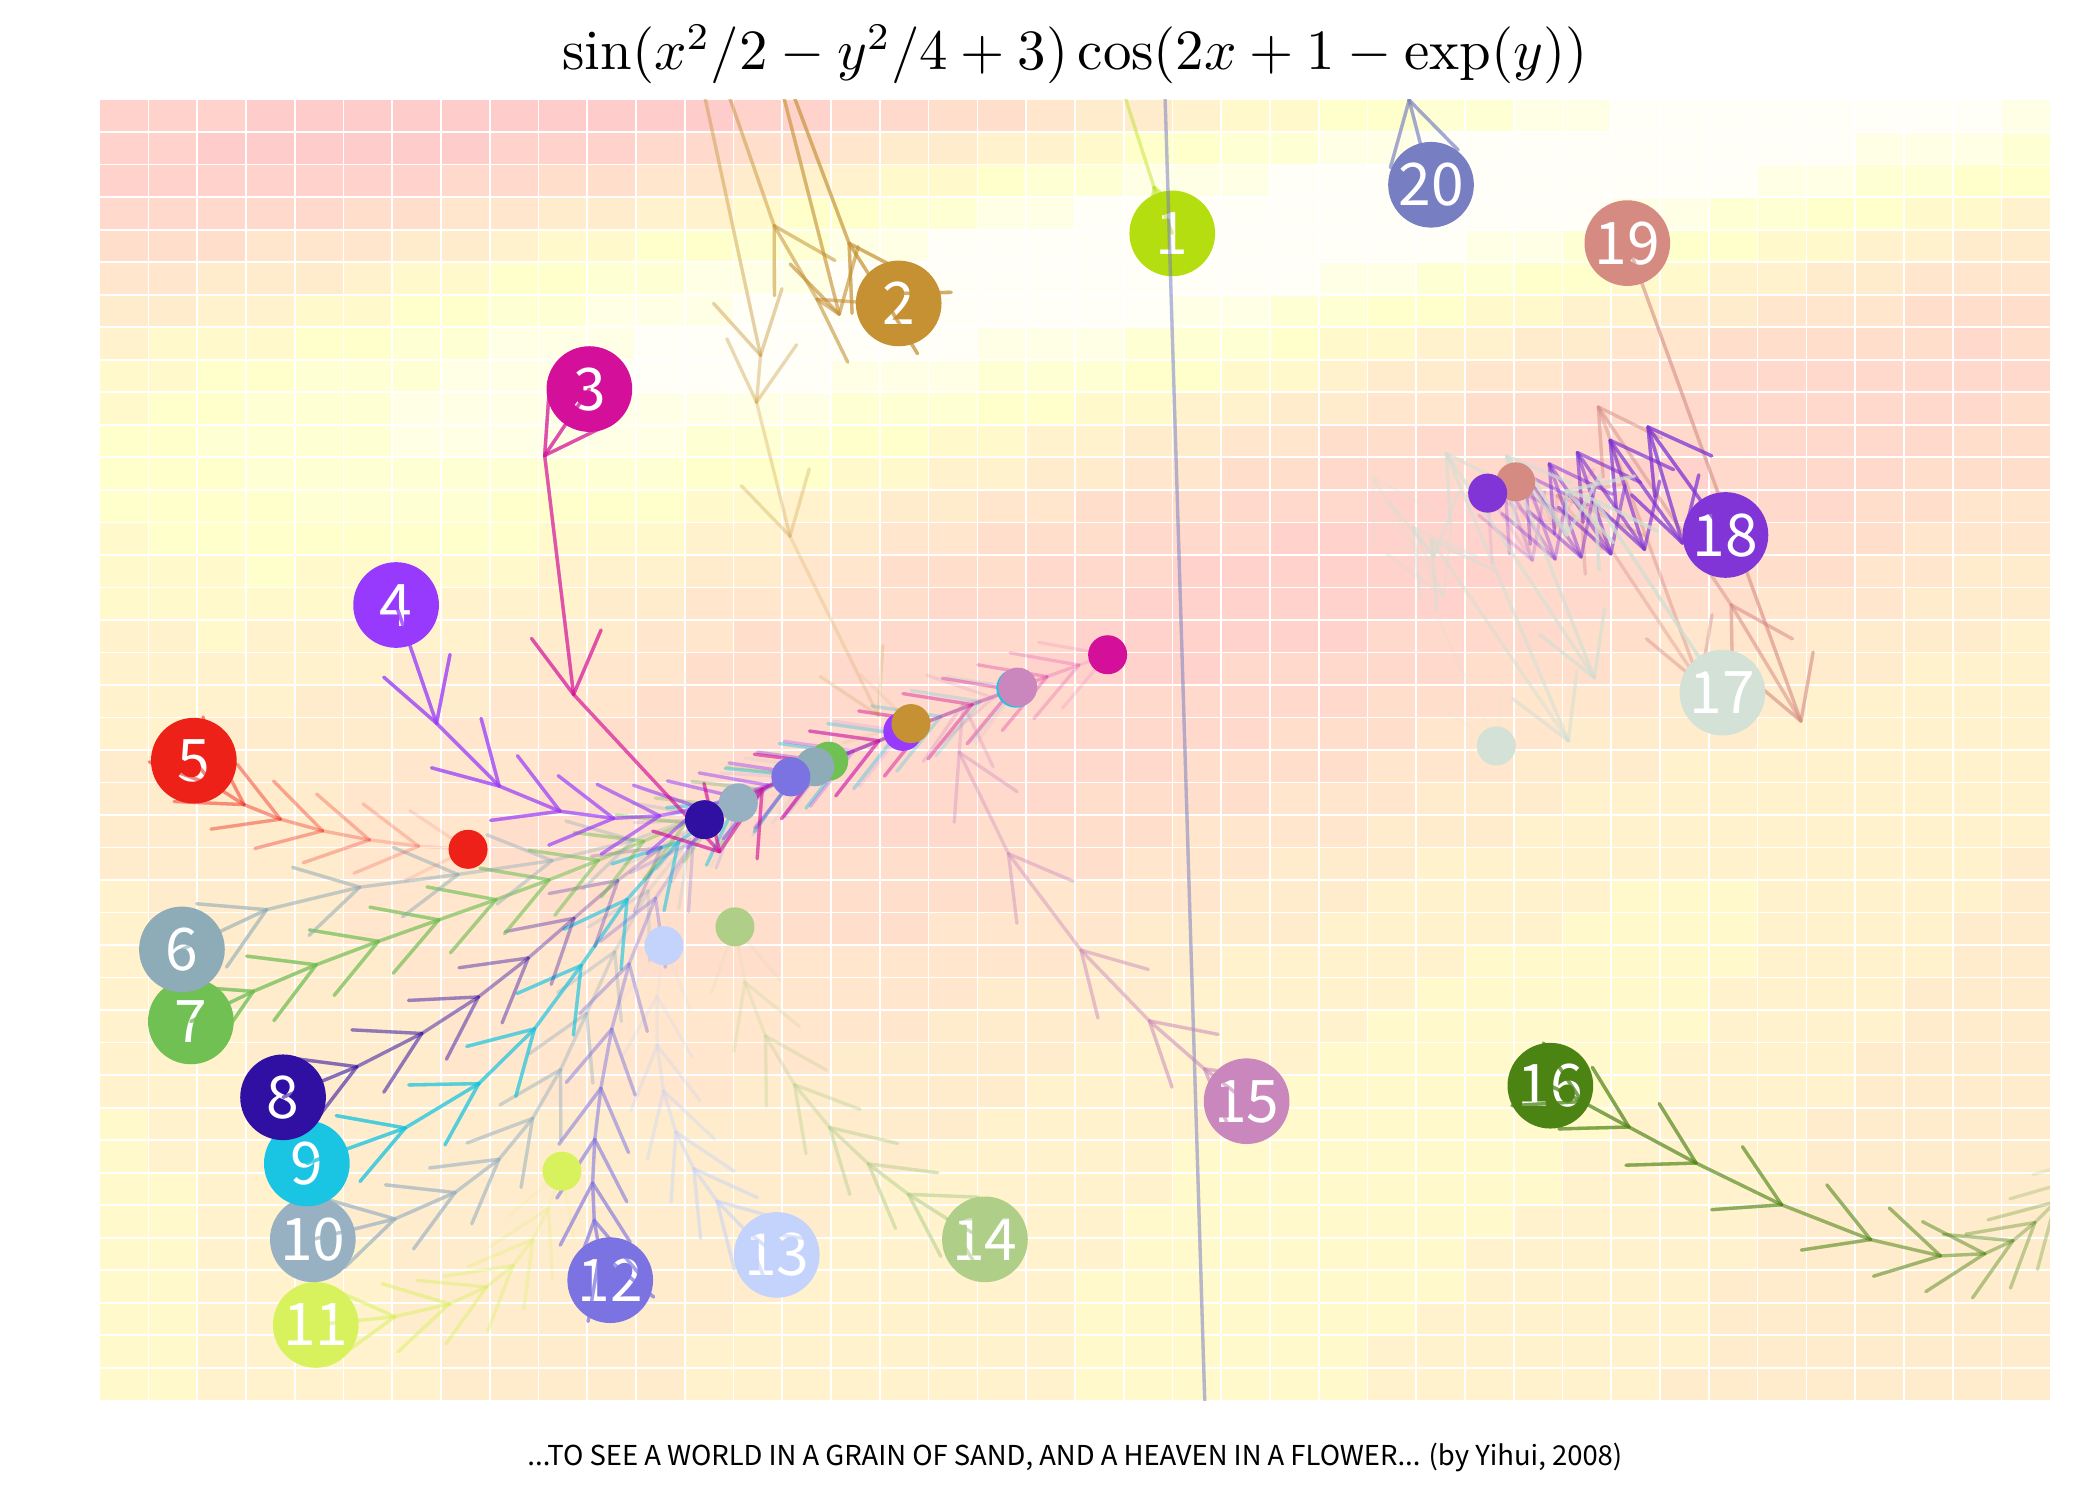
\includegraphics{elements_files/figure-latex/gradArrows-1} 

}

\caption[ 梯度下降算法的过程演示 ]{梯度下降算法的过程演示:对于同一个函数,我们选取 20 个迭代起点(外围大实心点),分别用不同的步长和迭代次数来进行迭代(里围相应颜色的小实心点为迭代终止位置)。从每一个起始点开始的迭代过程都由一系列箭头表示,最终这些箭头都大致指向同一个区域。本图是 2008 年作者为中国人民大学统计学院学生刊物《统计功课》设计的封面图形,底部一行附注``一沙一世界,一花一天堂'',取自英国诗人布莱克的诗《天真的预言》,意即仔细观察统计计算过程,会看到一个我们没注意过的微观世界。}\label{fig:gradArrows}
\end{figure}



\begin{Shaded}
\begin{Highlighting}[]
\FunctionTok{demo}\NormalTok{(}\StringTok{"signSTAT"}\NormalTok{, }\AttributeTok{package =} \StringTok{"MSG"}\NormalTok{)}
\end{Highlighting}
\end{Shaded}

\begin{figure}

{\centering 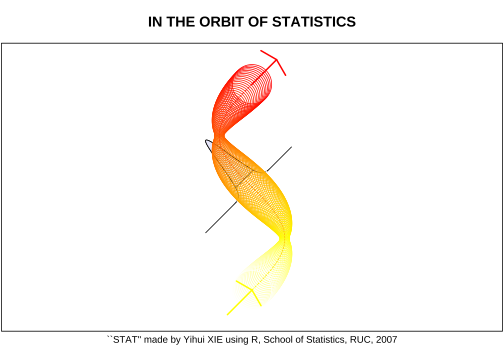
\includegraphics{elements_files/figure-latex/sign-stat-1} 

}

\caption[ 在统计学的轨道中(彩蛋)]{在统计学的轨道中(彩蛋):本图综合运用了折线、多边形、箭头、文本和圆圈等元素,它原本是作者于 2007 年为中国人民大学统计学院 06 级硕士班设计的一件班徽作品,但后来很多同学认为该图应重命名为``美人鱼图''。作者初衷是将``STAT''四个字母抽象表达为一些图形元素,例如图中一系列圆圈代表``S'',两端的箭头代表``T'',中间的正态分布曲线以及阴影部分代表``A''。}\label{fig:sign-stat}
\end{figure}



\section{小结}\label{ux5c0fux7ed3}

本章对图形元素的介绍就到此为止,后面章节的统计图形构造仍然会用到这些基础元素。具备这些低层函数的知识之后,只要我们不嫌麻烦,其实所有的统计图形都可以用它们的组合使用加上一定的统计计算而一步步构建出来。当然,一般也不会有人真用这样的方法去作图(练习除外)。我们指出这一点,也是为了说明,统计图形并没有任何神秘可言,随着对图形元素的绘制以及统计量的逐渐深入了解,当一幅统计图形摆在我们面前,我们也应该能如``庖丁解牛''一般洞穿其架构。例如,从纯粹作图的意义上来讲,直方图、条形图、棘状图和马赛克图不过是矩形,条件密度图和饼图是多边形,散点图和带状图是点,折线图和向日葵散点图是线段,等等。事实上,用 R 语言的作图功能作音乐五线谱、画地图、做动画等等,都不足为奇。本书 \ref{sec:animation} 小节中所谈到的统计学动画则是图形元素的另类应用,动画包 \textbf{animation} \citep{animation} 几乎完全是依靠统计计算与 R 基础图形系统而写成,例如前面提到的梯度下降算法的动画演示可以参考 \textbf{animation} 包中的 \texttt{grad.desc()} 函数。

前两章中,我们对 R 的作图基础元素和大部分参数都作了比较详细的介绍,大致掌握这些知识之后,下一章我们就可以正式进入本书的核心部分 --- 统计图形,在那些图形中,我们还会多次遇到这些基础知识的应用,到时读者可以再回顾复习。图 \ref{fig:sign-stat} 是本章最后一例``彩蛋'',供读者体会折线、多边形、箭头和文本等图形元素的用法。

\section{思考与练习}\label{ux601dux8003ux4e0eux7ec3ux4e60-2}

\begin{enumerate}
\def\labelenumi{\arabic{enumi}.}
\item
  彩色图形虽然在外观上很吸引人,但是它的一个局限是可能受客观条件限制而不能被打印出来(例如黑白打印机),我们在选取颜色的时候该如何平衡外观和打印效果?另外,男性和女性的色盲 / 色弱比例各是多少?(可以查阅维基百科:\url{https://en.wikipedia.org/wiki/Color_blindness})
\item
  图 \ref{fig:point-iris} 在点的样式选取上是否有明显的缺陷?或者说散点图中的点应该如何选取形状以使得各组点之间的外观差异尽量大?第 \ref{subsec:clear-symbols} 小节会对这个问题有详细评论。
\item
  当箭头角度参数 \texttt{angle} 为 \(90\,^{\circ}\)、\texttt{code} 参数为 3 时,箭头的形状是怎样的?这种形状是否和数学上的``区间''有类似之处?请考虑如何利用这种``双箭头''表达统计学中的置信区间。
\item
  利用三角形的边长关系画一个指北箭头如下

  \begin{center}
\includegraphics{elements_files/figure-latex/north-arrow-1} \end{center}
\item
  一些数学上函数可以产生有趣的``心形曲线'',例如在极坐标系下 \(r(\theta)=1-\sin(\theta)\) 生成的就是心形的曲线,笛卡尔坐标下方程 \((x^{2}+y^{2}-1)^{3}-x^{2}y^{3}=0\) 对应的解也可以形成心形曲线。这里我们考虑一种简单的心形曲线如下图所示:

  \begin{center}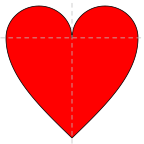
\includegraphics{elements_files/figure-latex/heart-curve-1} \end{center}

  这是个左右对称的形状,因此只需要知道左右任一侧的画法就知道整体画法了。实际上,右侧由上下两部分构成,上面是直径为 1 的半圆,下面是翻转了 \(90\,^{\circ}\) 的曲线 \(y=\sin(x),x\in[0,\pi/2]\)。请思考如何用多边形构造这个形状。MSG 包中的函数 \texttt{heart\_curve()} 可供参考。
\item
  温度计形状用来表达比例数据通常很形象,我们可以设定温度计的范围在 \([0,\,1]\) 之间,用汞柱的高度来表达比例。用 R 构造一支``温度计''很简单,如下图:这些温度计实际上由一个灰圆点、一个红圆点、一条灰线段和一条红线段叠加构成,红线段的长度表示比例大小,其它图形元素都只是背景。请尝试用四个图形元素构造温度计,注意这些图形元素的叠加顺序(例如红线必须在灰线之后画,否则会被覆盖)。\ref{sec:symbols} 小节的符号图中,``符号''的选项之一就是用温度计,但不如这里的温度计形象。对于追求细节完美的用户来说,这里线段末端的样式也值得注意,因为我们实际生活中看到的汞柱末端是弧形的,所以这里要是画成矩形就不合适了;线段末端的三种样式在 \ref{sec:par} 小节中有介绍。

  \begin{center}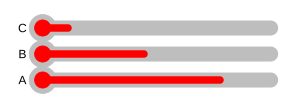
\includegraphics{elements_files/figure-latex/thermometer-demo-1} \end{center}
\end{enumerate}

\chapter{图库}\label{cha:gallery}

\begin{quote}
他解释说:``你要明白,我认为人的大脑原本像一间空空的屋子,必须有选择地用一些家具填满它。只有笨蛋才把他碰到的各种各样的破烂都塞进去。这样的话,那些可能用得上的知识就被挤了出来;或者,充其量也只是把那些破烂同其它东西混杂在一块儿。结果,在需要时却难得找到了。因此,一个善于工作的人,对于将什么东西纳入自己的头脑里是非常仔细的。他只会容纳那些工作时用得着的工具,而且又将这些工具分门别类,安排得井然有序。如果认为这间屋子的墙壁富有弹性,可以随意扩展,那就大错特错了。毫无疑问,总有一天,当你增加点滴知识时,却把从前熟悉的知识给忘记了。因此,不要让无用的信息挤掉那些有用的信息,这一点是至关重要的。''

\hspace*{\fill} --- 柯南·道尔《血字的研究》
\end{quote}

本章中,我们结合 R 语言中的相关函数以及数据实例对各种统计图形依次作出介绍。从第 \ref{sec:hist} 节到 \ref{sec:pie} 节的所有图形都是基于 \textbf{graphics} 包所作,其后的图形均来自于其它函数包。图形的介绍顺序大致按函数的字母序,但直方图、箱线图和散点图等常见图形放在前面,而饼图被有意安排在最后。

\section{直方图}\label{sec:hist}

直方图(Histogram)是展示连续数据分布最常用的工具,它本质上是对密度函数的一种估计。在介绍作图方法之前我们有必要先了解一下它的基本数学思想,本节仅作简要介绍,
详细的数学理论参见 \citet{Scott92}。

我们知道,对于连续随机变量来说,其密度函数即为分布函数的导数:

\begin{equation} 
f(x)=F'(x)=\lim_{h\rightarrow0}\frac{F(x+h)-F(x)}{h}
\label{eq:density}
\end{equation}

因此我们不妨自然而然地从分布函数的估计出发得到密度函数的估计。当我们拿到一批数据 \(X_1,X_2,\ldots,X_n\) 时,我们最容易想到的分布函数估计就是经验分布函数:

\begin{equation} 
\hat{F}_{n}(x)=\frac{1}{n}\sum_{i=1}^{n}\mathbf{I}(X_{i}\leq x)
\label{eq:empirical}
\end{equation}

其中 \(\mathbf{I}(\cdot)\) 为示性函数;结合公式 \eqref{eq:density} 和 \eqref{eq:empirical} 以及示性函数的性质,我们可以直接得到以下密度函数估计:

\begin{equation} 
\hat{f}_{n}(x)=\lim_{h\rightarrow0}\frac{1}{n}\sum_{i=1}^{n}\frac{\mathbf{I}(x<X_{i}\leq x+h)}{h}
\label{eq:den-est}
\end{equation}

公式 \eqref{eq:den-est} 实际上已经给出了直方图作为密度函数估计工具的基本思想:划分区间并计数有多少数据点落入该区间。实际数据不可能无限稠密,因此 \(h\rightarrow0\) 的条件往往是不可能实现的,于是我们退而求其次,只是在某一些区间段里面估计区间上的密度。首先我们将实数轴划分为若干宽度为 \(h\) 的区间(我们称 \(h\) 为``窗宽''):

\begin{equation} 
b_{1}<b_{2}<\cdots<b_{j}<b_{j+1}<\cdots;\;b_{j+1}-b_{j}=h,\,j=1,2,\cdots
\label{eq:den-est2}
\end{equation}

然后根据以下直方图密度估计表达式计算区间 \((b_j,b_{j+1}]\) 上的密度估计值:

\begin{equation} 
\hat{f}_{n}(x)=\frac{1}{nh}\sum_{i=1}^{n}\mathbf{I}(b_{j}<X_{i}\leq b_{j+1});\;x\in(b_{j},b_{j+1}]
\label{eq:den-formula}
\end{equation}

最后我们将密度估计值以矩形的形式表示出来,就完成了直方图的基本制作。当然我们没有必要使用这样原始的方式制作直方图,R 中提供了 \texttt{hist()} 函数,其默认用法如下:

\begin{Shaded}
\begin{Highlighting}[]
\FunctionTok{usage}\NormalTok{(hist.default)}
\end{Highlighting}
\end{Shaded}

\begin{verbatim}
## ## Default S3 method:
## hist(x, breaks = "Sturges", freq = NULL, probability = !freq,
##   include.lowest = TRUE, right = TRUE, fuzz = 1e-07, density = NULL,
##   angle = 45, col = "lightgray", border = NULL,
##   main = paste("Histogram of", xname), xlim = range(breaks), ylim = NULL,
##   xlab = xname, ylab, axes = TRUE, plot = TRUE, labels = FALSE, nclass = NULL,
##   warn.unused = TRUE, ...)
\end{verbatim}

其中, \texttt{x} 为欲估计分布的数值向量;\texttt{breaks} 决定了计算分段区间的方法,它可以是一个向量(依次给出区间端点),或者一个数字(决定拆分为多少段),或者一个字符串(给出计算划分区间的算法名称),或者一个函数(给出划分区间个数的方法),区间的划分直接决定了直方图的形状,因此这个参数是非常关键的; \texttt{freq} 和 \texttt{probability} 参数均取逻辑值(二者互斥),前者决定是否以频数作图,后者决定是否以概率密度作图(这种情况下矩形面积为 1); \texttt{labels} 为逻辑值,决定是否将频数的数值添加到矩形条的上方;其它参数诸如 \texttt{density} 、 \texttt{angle} 、 \texttt{border} 均可参见低层作图函数''矩形''( \texttt{rect()} ,\ref{sec:polygon} 节)。





\begin{Shaded}
\begin{Highlighting}[]
\FunctionTok{par}\NormalTok{(}\AttributeTok{mfrow =} \FunctionTok{c}\NormalTok{(}\DecValTok{2}\NormalTok{, }\DecValTok{2}\NormalTok{), }\AttributeTok{mar =} \FunctionTok{c}\NormalTok{(}\DecValTok{2}\NormalTok{, }\DecValTok{3}\NormalTok{, }\DecValTok{2}\NormalTok{, .}\DecValTok{5}\NormalTok{), }\AttributeTok{mgp =} \FunctionTok{c}\NormalTok{(}\DecValTok{2}\NormalTok{, .}\DecValTok{5}\NormalTok{, }\DecValTok{0}\NormalTok{))}
\FunctionTok{data}\NormalTok{(geyser, }\AttributeTok{package =} \StringTok{"MASS"}\NormalTok{)}
\FunctionTok{hist}\NormalTok{(geyser}\SpecialCharTok{$}\NormalTok{waiting, }\AttributeTok{main =} \StringTok{"(1) freq = TRUE"}\NormalTok{, }\AttributeTok{xlab =} \StringTok{"waiting"}\NormalTok{)}
\FunctionTok{hist}\NormalTok{(geyser}\SpecialCharTok{$}\NormalTok{waiting, }\AttributeTok{freq =} \ConstantTok{FALSE}\NormalTok{, }\AttributeTok{xlab =} \StringTok{"waiting"}\NormalTok{, }\AttributeTok{main =} \StringTok{"(2) freq = FALSE"}\NormalTok{)}
\FunctionTok{hist}\NormalTok{(geyser}\SpecialCharTok{$}\NormalTok{waiting, }\AttributeTok{breaks =} \DecValTok{5}\NormalTok{, }\AttributeTok{density =} \DecValTok{10}\NormalTok{, }\AttributeTok{xlab =} \StringTok{"waiting"}\NormalTok{, }\AttributeTok{main =} \StringTok{"(3) breaks = 5"}\NormalTok{)}
\FunctionTok{hist}\NormalTok{(geyser}\SpecialCharTok{$}\NormalTok{waiting, }\AttributeTok{breaks =} \DecValTok{40}\NormalTok{, }\AttributeTok{col =} \StringTok{"red"}\NormalTok{, }\AttributeTok{xlab =} \StringTok{"waiting"}\NormalTok{, }\AttributeTok{main =} \StringTok{"(4) breaks = 40"}\NormalTok{)}

\FunctionTok{library}\NormalTok{(ggplot2)}
\FunctionTok{library}\NormalTok{(cowplot)}
\NormalTok{p }\OtherTok{\textless{}{-}} \FunctionTok{ggplot}\NormalTok{(}\FunctionTok{aes}\NormalTok{(waiting), }\AttributeTok{data =}\NormalTok{ geyser)}
\NormalTok{p1 }\OtherTok{\textless{}{-}}\NormalTok{ p }\SpecialCharTok{+} \FunctionTok{geom\_histogram}\NormalTok{(}\AttributeTok{breaks =} \FunctionTok{seq}\NormalTok{(}\DecValTok{40}\NormalTok{, }\DecValTok{110}\NormalTok{, }\AttributeTok{by =} \DecValTok{5}\NormalTok{))}
\NormalTok{p2 }\OtherTok{\textless{}{-}}\NormalTok{ p }\SpecialCharTok{+} \FunctionTok{geom\_histogram}\NormalTok{(}\AttributeTok{breaks =} \FunctionTok{seq}\NormalTok{(}\DecValTok{40}\NormalTok{, }\DecValTok{110}\NormalTok{, }\AttributeTok{by =} \DecValTok{5}\NormalTok{), }\FunctionTok{aes}\NormalTok{(}\AttributeTok{y =} \FunctionTok{after\_stat}\NormalTok{(density)))}
\NormalTok{p3 }\OtherTok{\textless{}{-}}\NormalTok{ p }\SpecialCharTok{+} \FunctionTok{geom\_histogram}\NormalTok{(}\AttributeTok{breaks =} \FunctionTok{seq}\NormalTok{(}\DecValTok{40}\NormalTok{, }\DecValTok{110}\NormalTok{, }\AttributeTok{by =} \DecValTok{10}\NormalTok{))}
\NormalTok{p4 }\OtherTok{\textless{}{-}}\NormalTok{ p }\SpecialCharTok{+} \FunctionTok{geom\_histogram}\NormalTok{(}\AttributeTok{breaks =} \FunctionTok{seq}\NormalTok{(}\DecValTok{42}\NormalTok{, }\DecValTok{108}\NormalTok{, }\AttributeTok{by =} \DecValTok{2}\NormalTok{), }\AttributeTok{fill =} \StringTok{"red"}\NormalTok{, }\AttributeTok{color =} \StringTok{"black"}\NormalTok{)}
\FunctionTok{plot\_grid}\NormalTok{(p1, p2, p3, p4, }\AttributeTok{labels =} \FunctionTok{c}\NormalTok{(}
  \StringTok{"(1) freq = TRUE"}\NormalTok{,}
  \StringTok{"(2) freq = FALSE"}\NormalTok{,}
  \StringTok{"(3) breaks = 5"}\NormalTok{,}
  \StringTok{"(4) breaks = 40"}
\NormalTok{), }\AttributeTok{ncol =} \DecValTok{2}\NormalTok{)}
\end{Highlighting}
\end{Shaded}

\begin{figure}

{\centering 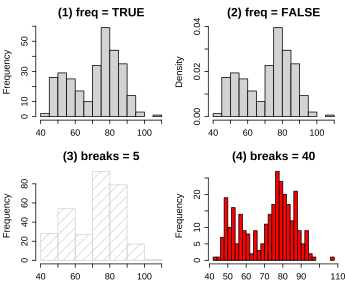
\includegraphics[width=0.7\linewidth]{gallery_files/figure-latex/hist-geyser-1} 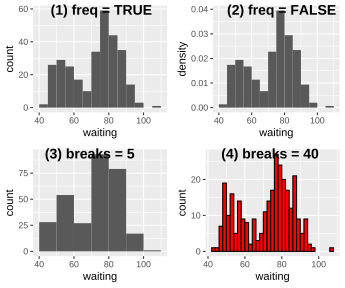
\includegraphics[width=0.7\linewidth]{gallery_files/figure-latex/hist-geyser-2} 

}

\caption[喷泉间隔时间直方图]{喷泉间隔时间直方图:(1)使用默认参数值(作频数图);(2)概率密度直方图;(3)减小区间段数,直方图看起来更平滑(偏差大,方差小);(4)增大区间段数,直方图更突兀(偏差小,方差大)}\label{fig:hist-geyser}
\end{figure}

我们以黄石国家公园喷泉数据 \texttt{geyser} \citep{Venables02} 为例。图 \ref{fig:hist-geyser} 展示了喷泉喷发间隔时间的分布情况。(1)和(2)中的直方图看起来形状完全一样,区别仅仅是前者为频数图,后者为密度图。二者在统计量上仅相差一个常数倍,但密度直方图的一个便利之处在于它可以方便地添加密度曲线,用以辅助展示数据的统计分布(图 \ref{fig:hist-density} 即为一个示例);(3)和(4)的区别在于区间划分段数,我们可以很清楚看出区间划分的多少对直方图的直接影响。关于区间划分的一些讨论可以参考 \citet{Venables02},这里我们需要特别指出的是,直方图的理论并非想象中或看起来的那么简单,窗宽也并非可以任意选择,不同的窗宽或区间划分方法会导致不同的估计误差。关于这一点,Excel 的直方图可以说是非常不可靠的,因为它把区间的划分方法完全交给了用户去选择,这样随意制作出来的直方图很可能会导致大的估计误差、掩盖数据的真实分布情况。另外一点需要提醒的是关于直方图中的密度曲线,SPSS 软件在绘制直方图时会有选项提示是否添加正态分布密度曲线,这也是完全的误导,因为数据不一定来自正态分布,添加正态分布的密度曲线显然是不合理的,相比之下,图 \ref{fig:hist-density} 的做法才是真正从数据本来的分布出发得到的密度曲线。





\begin{Shaded}
\begin{Highlighting}[]
\FunctionTok{demo}\NormalTok{(}\StringTok{"hist\_geyser"}\NormalTok{, }\AttributeTok{package =} \StringTok{"MSG"}\NormalTok{)}
\NormalTok{df }\OtherTok{\textless{}{-}} \FunctionTok{data.frame}\NormalTok{(}
  \AttributeTok{x =} \FunctionTok{seq}\NormalTok{(}\DecValTok{40}\NormalTok{, }\DecValTok{110}\NormalTok{, }\DecValTok{5}\NormalTok{), }\AttributeTok{y =} \DecValTok{0}\NormalTok{,}
  \AttributeTok{xend =} \FunctionTok{seq}\NormalTok{(}\DecValTok{40}\NormalTok{, }\DecValTok{110}\NormalTok{, }\DecValTok{5}\NormalTok{), }\AttributeTok{yend =}\NormalTok{ ht}
\NormalTok{)}
\NormalTok{p2 }\SpecialCharTok{+} \FunctionTok{geom\_density}\NormalTok{(}\AttributeTok{fill =} \StringTok{"lightgray"}\NormalTok{, }\AttributeTok{color =} \StringTok{"black"}\NormalTok{) }\SpecialCharTok{+}
  \FunctionTok{geom\_segment}\NormalTok{(}\FunctionTok{aes}\NormalTok{(}\AttributeTok{x =}\NormalTok{ x, }\AttributeTok{y =}\NormalTok{ y, }\AttributeTok{xend =}\NormalTok{ xend, }\AttributeTok{yend =}\NormalTok{ yend),}
    \AttributeTok{data =}\NormalTok{ df, }\AttributeTok{lty =} \DecValTok{3}
\NormalTok{  )}
\end{Highlighting}
\end{Shaded}

\begin{figure}

{\centering 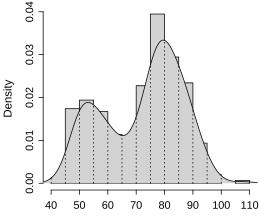
\includegraphics[width=0.35\linewidth]{gallery_files/figure-latex/hist-density-1} 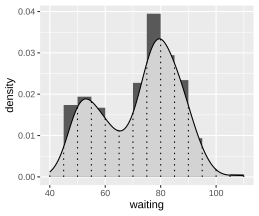
\includegraphics[width=0.35\linewidth]{gallery_files/figure-latex/hist-density-2} 

}

\caption[直方图与密度曲线的结合]{直方图与密度曲线的结合:借助函数 \texttt{density()} 可以计算出数据的核密度估计,然后利用低层作图函数 \texttt{lines()} 将核密度估计曲线添加到直方图中。}\label{fig:hist-density}
\end{figure}

直方图函数在作图完毕之后会有一些计算返回值,这些值对于进一步的作图或者分析很有用,例如区间划分端点、频数(或密度)、区间中点等等,这些信息可以被灵活应用在图形定制上
(例如图 \ref{fig:layout-margin})。

由于直方图需要对连续型数据做离散分组,因此它有一个明显的缺点,就是它的形状依赖于分组的端点,例如若有好几个相同的数值正好处在分组端点上,那么我们只要稍微向左或向右移动一下分组端点,这些数据点就会被划分入不同的区间,导致矩形条的高度变化。\citet{Scott92} 提出了一种解决这种直方图不稳定性问题的办法叫``移动平均直方图''(Average Shifted Histogram,简称 ASH),它的思想是使用一系列移动的区间去划分数据,比如 \((b_1+ih/n,b_2+ih/n,\ldots,b_n+ih/n)\),\(i=0,\cdots,n-1\),最后将这 \(n\) 种划分方法的频数结果''平均''起来,就得到了 ASH 图,这样有效避免了边界点的归属问题。然而,在核密度估计理论已经非常完备的今天,我们几乎没有必要再用这种技巧去克服原来的问题了,毕竟 ASH 与核密度估计比起来显得还是太粗糙。图 \ref{fig:hist-density} 的核密度曲线基于函数 \texttt{density()} 计算而来,它的参数包括核函数和窗宽等,实际应用中我们可能需要尝试不同的核函数以及窗宽值,\citet{Venables02} 第 5.6 小节介绍了一些选择的经验可供参考。

\section{茎叶图}\label{ux830eux53f6ux56fe}

茎叶图(Stem-and-Leaf Plot)与直方图的功能类似,也是展示数据密度的一种工具,但相比之下茎叶图对密度的刻画显得非常粗略,而且对原始数据通常会作舍入处理,它只是在早期计算机尚不发达时对于手工整理数据来说比较方便。茎叶图的整体形状如同植物的茎和叶,对于一个数据,通常取其 \(10^n\) 部分为茎(\(n\) 视所有数据的数量级而定),剩下的尾数为叶,放置于茎旁,这样每隔 \(m10^n\) 就对数据作一次归类汇总,将落入区间 \([km10^{n},\ (k+1)m10^{n}]\) 的数据汇集为叶子(\(k,m\) 为整数,\(m\) 通常取 1,\(k=1,2,3,\cdots\)),我们不妨称这种区间为一个``节'',节的长度与直方图的``窗宽''本质上是同样的概念。显然,叶子越长则表明该节上数据频数越高。

R 中茎叶图的函数为 \texttt{stem()},其用法为:

\begin{Shaded}
\begin{Highlighting}[]
\FunctionTok{usage}\NormalTok{(stem)}
\end{Highlighting}
\end{Shaded}

\begin{verbatim}
## stem(x, scale = 1, width = 80, atom = 1e-08)
\end{verbatim}

参数 \texttt{scale} 控制着 \(m\),即节与节之间的长度( \texttt{scale} 越大则 \(m\) 越小); \texttt{width} 控制了茎叶图的宽度,若叶子的长度超出了这个设置,则叶子会被截取到长度 \texttt{width} ,然后以一个整数表示后面尚有多少片叶子没有被画出来。

下面我们以 \textbf{datasets} 包中 \texttt{islands} 数据为例说明茎叶图的作法。该数据记录了世界上各大陆地块的面积大小,原始数据前 10 条如下(单位:千平方英里):

\begin{Shaded}
\begin{Highlighting}[]
\FunctionTok{head}\NormalTok{(islands, }\DecValTok{10}\NormalTok{)}
\end{Highlighting}
\end{Shaded}

\begin{verbatim}
##       Africa   Antarctica         Asia    Australia Axel Heiberg       Baffin 
##        11506         5500        16988         2968           16          184 
##        Banks       Borneo      Britain      Celebes 
##           23          280           84           73
\end{verbatim}

可以看出,以上数据中最大的数量级为 \(10^{4}\),而大部分数据的数量级集中在 \(10^{1}\),因此茎上的数量级取作 \(10^{3}\) 相对比较合适---更大的数量级会导致茎的节数非常少,对分布的刻画过于粗略;而更小的数量级会导致节数过多,使得茎叶图几乎退化为数据的原始表示,这样也难以看出数据的集中趋势。下图展示了 48 块大陆块面积的分布,该茎叶图窗宽为 \(2\times10^{3}\),图中注明了原始数据小数点位置在 \texttt{\textbar{}} 后面三位数处,因此我们从图中``还原''原始数据时,需要用(``茎的区间`+'叶'')\(\times10^{3}\)。

\begin{Shaded}
\begin{Highlighting}[]
\FunctionTok{stem}\NormalTok{(islands)}
\end{Highlighting}
\end{Shaded}

\begin{verbatim}
## 
##   The decimal point is 3 digit(s) to the right of the |
## 
##    0 | 00000000000000000000000000000111111222338
##    2 | 07
##    4 | 5
##    6 | 8
##    8 | 4
##   10 | 5
##   12 | 
##   14 | 
##   16 | 0
\end{verbatim}

\begin{Shaded}
\begin{Highlighting}[]
\FunctionTok{stem}\NormalTok{(islands, }\AttributeTok{width =} \DecValTok{20}\NormalTok{)}
\end{Highlighting}
\end{Shaded}

\begin{verbatim}
## 
##   The decimal point is 3 digit(s) to the right of the |
## 
##    0 | 00000000+21
##    2 | 07
##    4 | 5
##    6 | 8
##    8 | 4
##   10 | 5
##   12 | 
##   14 | 
##   16 | 0
\end{verbatim}

\begin{Shaded}
\begin{Highlighting}[]
\CommentTok{\# 可以增大窗宽 stem(islands, scale = 2) 看看效果}
\end{Highlighting}
\end{Shaded}

可以明显看出,这些面积数据是严重右偏的,即:少数陆地块的面积非常大,而大多数陆地块的面积相对来说都很小。事实上,主要是七大洲的大陆块面积非常大,而其它岛屿诸如海南岛、帝汶岛、九洲岛等面积都相对较小。

我们以上图为例说明一下茎叶图的制作过程及其相应解释。首先我们将原始数据除以 \(10^{3}\),并四舍五入到小数点后的一位数:

\begin{Shaded}
\begin{Highlighting}[]
\CommentTok{\# 去掉陆地名称以便显示数据}
\FunctionTok{unname}\NormalTok{(}\FunctionTok{sort}\NormalTok{(}\FunctionTok{round}\NormalTok{(islands }\SpecialCharTok{/} \DecValTok{1000}\NormalTok{, }\DecValTok{1}\NormalTok{)))}
\end{Highlighting}
\end{Shaded}

\begin{verbatim}
##  [1]  0.0  0.0  0.0  0.0  0.0  0.0  0.0  0.0  0.0  0.0  0.0  0.0  0.0  0.0  0.0
## [16]  0.0  0.0  0.0  0.0  0.0  0.0  0.0  0.0  0.0  0.0  0.0  0.0  0.0  0.0  0.1
## [31]  0.1  0.1  0.1  0.1  0.1  0.2  0.2  0.2  0.3  0.3  0.8  3.0  3.7  5.5  6.8
## [46]  9.4 11.5 17.0
\end{verbatim}

然后从 0 到 \(18\times10^{3}\)、以 \(2\times10^{3}\) 为窗宽,分段整理数据,每一段(节)中依次放置落入该段的数据的小数位,堆砌起来便形成了茎叶图的叶子。例如 \(11.5\) 落入了 \([10,12]\) 的区间,我们就将尾数 5 放在 10 的右边;类似地,17.0 在 \([16,18]\) 之间,我们将 0 放在 16 右边;关于茎叶图顶部的一长串 0 的解释此处不再赘述。

下图是利用泊松分布(\(\lambda=10\))随机数生成的茎叶图,可以看出数据密度在 10 附近最高,这与理论相符。由于窗宽为 1,不存在舍入问题,所以图形可以还原到原始数据,请读者自行对应数据观察茎叶图。

\begin{Shaded}
\begin{Highlighting}[]
\CommentTok{\# 均值 lambda 为 10 的泊松分布随机数}
\FunctionTok{sort}\NormalTok{(x }\OtherTok{\textless{}{-}} \FunctionTok{rpois}\NormalTok{(}\DecValTok{80}\NormalTok{, }\AttributeTok{lambda =} \DecValTok{10}\NormalTok{))}
\end{Highlighting}
\end{Shaded}

\begin{verbatim}
##  [1]  3  4  5  5  5  6  6  6  7  7  7  7  7  7  7  7  8  8  8  8  8  9  9  9  9
## [26]  9  9  9  9  9 10 10 10 10 10 10 10 10 10 10 10 10 10 10 10 10 10 10 11 11
## [51] 11 11 11 11 11 12 12 12 12 12 12 12 12 12 12 12 13 13 13 14 14 15 15 15 15
## [76] 15 16 17 17 18
\end{verbatim}

\begin{Shaded}
\begin{Highlighting}[]
\FunctionTok{stem}\NormalTok{(x, }\AttributeTok{scale =} \DecValTok{2}\NormalTok{)}
\end{Highlighting}
\end{Shaded}

\begin{verbatim}
## 
##   The decimal point is at the |
## 
##    3 | 0
##    4 | 0
##    5 | 000
##    6 | 000
##    7 | 00000000
##    8 | 00000
##    9 | 000000000
##   10 | 000000000000000000
##   11 | 0000000
##   12 | 00000000000
##   13 | 000
##   14 | 00
##   15 | 00000
##   16 | 0
##   17 | 00
##   18 | 0
\end{verbatim}

经过前面的说明,现在我们不妨将茎叶图简单理解为横放着的直方图,只是茎叶图通常都以某个便利的整数为窗宽,不如直方图那样精细。此外,茎叶图曾经的优势(简单、可手工绘制)在今天这个计算机时代也显得并不突出,因此,除非特殊情况,我们建议主要使用直方图作为密度函数估计工具。

\section{箱线图}\label{sec:boxplot}

箱线图(Box Plot 或 Box-and-Whisker Plot)主要是从四分位数的角度出发
描述数据的分布,它通过最大值(\(Q_4\))、上四分位数(\(Q_3\))、中位数(\(Q_2\))、下四分位数(\(Q_1\))和最小值(\(Q_0\))五处位置来获取一维数据的分布概况。我们知道,这五处位置之间依次包含了四段数据,每段中数据量均为总数据量的 \(1/4\)。通过每一段数据占据的长度,我们可以大致推断出数据的集中或离散趋势(长度越短,说明数据在该区间上越密集,反之则稀疏)。

R 中相应的函数为 \texttt{boxplot()},其用法如下:

\begin{Shaded}
\begin{Highlighting}[]
\CommentTok{\# 默认用法}
\FunctionTok{usage}\NormalTok{(boxplot.default)}
\end{Highlighting}
\end{Shaded}

\begin{verbatim}
## ## Default S3 method:
## boxplot(x, ..., range = 1.5, width = NULL, varwidth = FALSE, notch = FALSE,
##   outline = TRUE, names, plot = TRUE, border = par("fg"), col = "lightgray",
##   log = "", pars = list(boxwex = 0.8, staplewex = 0.5, outwex = 0.5),
##   ann = !add, horizontal = FALSE, add = FALSE, at = NULL)
\end{verbatim}

\begin{Shaded}
\begin{Highlighting}[]
\CommentTok{\# 公式用法}
\FunctionTok{usage}\NormalTok{(graphics}\SpecialCharTok{:::}\NormalTok{boxplot.formula)}
\end{Highlighting}
\end{Shaded}

\begin{verbatim}
## ## S3 method for class 'formula'
## boxplot(formula, data = NULL, ..., subset, na.action = NULL,
##   xlab = mklab(y_var = horizontal), ylab = mklab(y_var = !horizontal),
##   add = FALSE, ann = !add, horizontal = FALSE, drop = FALSE, sep = ".",
##   lex.order = FALSE)
\end{verbatim}

因为 \texttt{boxplot()} 是一个泛型函数,所以它可以适应不同的参数类型。目前它支持两种参数类型:公式( \texttt{formula} )和数据,后者对我们来说可能更容易理解(给一批数据、作相应的箱线图),而前者在某些情况下更为方便,后面我们会举例说明。参数 \texttt{x} 为一个数值向量或者列表,若为列表则对列表中每一个子对象依次作出箱线图; \texttt{range} 是一个延伸倍数,决定了箱线图的末端(须)延伸到什么位置,这主要是考虑到离群点的原因,在数据中存在离群点的情况下,将箱线图末端直接延伸到最大值和最小值对描述数据分布来说并不合适(图形缺乏稳健性),所以 R 中的箱线图默认只将图形延伸到离箱子两端 \(\mathrm{range}\times(Q_3-Q_1)\) 处,即上下四分位数分别加/减内四分位距(Interquartile
Range,简称 \(\text{IQR}\equiv Q_3-Q_1\))的倍数,超过这个范围的数据点就被视作离群点,在图中直接以点的形式表示出来; \texttt{width} 给定箱子的宽度; \texttt{varwidth} 为逻辑值,若为 \texttt{TRUE},那么箱子的宽度与样本量的平方根成比例,这在多批数据同时画多个箱线图时比较有用,能进一步反映出样本量的大小; \texttt{notch} 也是一个有用的逻辑参数,它决定了是否在箱子上画凹槽,凹槽所表示的实际上是中位数的一个区间估计,其计算式为 \(Q_2+/-1.58\mathrm{IQR}/\sqrt{n}\)
\citep{McGill78, Chambers83},区间置信水平为 95\%,在比较两组数据中位数差异时,我们只需要观察箱线图的凹槽是否有重叠部分,若两个凹槽互不交叠,那么说明这两组数据的中位数有显著差异(P 值小于 0.05); \texttt{horizontal} 为逻辑值,设定箱线图是否水平放置; \texttt{add} 设置是否将箱线图添加到现有图形上(例:图 \ref{fig:symbols-pop});其它参数诸如设置箱子颜色、位置、更详细的宽度等参见 \texttt{?boxplot}。





\begin{Shaded}
\begin{Highlighting}[]
\FunctionTok{boxplot}\NormalTok{(count }\SpecialCharTok{\textasciitilde{}}\NormalTok{ spray, }\AttributeTok{data =}\NormalTok{ InsectSprays,}
        \AttributeTok{col =} \StringTok{"lightgray"}\NormalTok{, }\AttributeTok{horizontal =} \ConstantTok{TRUE}\NormalTok{, }\AttributeTok{pch =} \DecValTok{4}\NormalTok{)}
\FunctionTok{ggplot}\NormalTok{(}\FunctionTok{aes}\NormalTok{(}\AttributeTok{y =}\NormalTok{ count, }\AttributeTok{x =}\NormalTok{ spray), }\AttributeTok{data =}\NormalTok{ InsectSprays) }\SpecialCharTok{+}
  \FunctionTok{geom\_boxplot}\NormalTok{(}\AttributeTok{outlier.shape =} \DecValTok{4}\NormalTok{) }\SpecialCharTok{+}
  \FunctionTok{coord\_flip}\NormalTok{()}
\end{Highlighting}
\end{Shaded}

\begin{figure}

{\centering 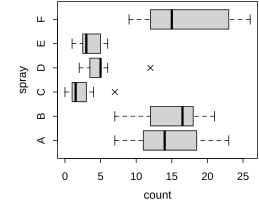
\includegraphics{gallery_files/figure-latex/insects-boxplot-1} 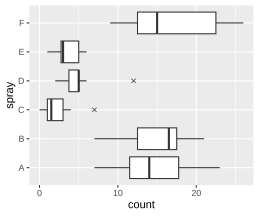
\includegraphics{gallery_files/figure-latex/insects-boxplot-2} 

}

\caption[各种杀虫剂下昆虫数目的箱线图]{昆虫数目箱线图:六种杀虫剂下昆虫的数目分布。}\label{fig:insects-boxplot}
\end{figure}

绘制单个箱线图时只需要给 \texttt{boxplot()} 传入一个数值向量即可,如:\texttt{boxplot(rnorm(100))};这里我们主要使用公式型的参数,以 \textbf{datasets} 包中的杀虫剂数据 \texttt{InsectSprays} 为例。该数据有两列,第一列为昆虫数目,第二列为杀虫剂种类(ABCDEF),这里是随机抽取的 10 列数据:

\begin{Shaded}
\begin{Highlighting}[]
\NormalTok{InsectSprays[}\FunctionTok{sample}\NormalTok{(}\FunctionTok{nrow}\NormalTok{(InsectSprays), }\DecValTok{10}\NormalTok{), ]}
\end{Highlighting}
\end{Shaded}

\begin{verbatim}
##    count spray
## 38     5     D
## 44     5     D
## 25     0     C
## 33     3     C
## 61    11     F
## 18    14     B
## 47     2     D
## 12    13     A
## 21    19     B
## 28     2     C
\end{verbatim}

为了了解杀虫剂的效果,我们需要对各种杀虫剂下昆虫的数目作出比较。图 \ref{fig:insects-boxplot} 是一个简单的箱线图展示,不难看出,除了 B 和 D 对应的昆虫数据呈左偏形态外,其它组均有右偏趋势,看起来各组数据的平均水平差异比较明显;另外注意观察图中的两个离群点(以 ``\(\times\)'' 表示)。总体看来,C 的效果最好。事实上,我们可以对这个数据作方差分析,检验杀虫剂类型对昆虫数目是否有显著影响:

\begin{Shaded}
\begin{Highlighting}[]
\NormalTok{insects.aov }\OtherTok{\textless{}{-}} \FunctionTok{aov}\NormalTok{(count }\SpecialCharTok{\textasciitilde{}}\NormalTok{ spray, }\AttributeTok{data =}\NormalTok{ InsectSprays)}
\FunctionTok{summary}\NormalTok{(insects.aov)}
\end{Highlighting}
\end{Shaded}

\begin{verbatim}
##             Df Sum Sq Mean Sq F value Pr(>F)    
## spray        5   2669   533.8    34.7 <2e-16 ***
## Residuals   66   1015    15.4                   
## ---
## Signif. codes:  0 '***' 0.001 '**' 0.01 '*' 0.05 '.' 0.1 ' ' 1
\end{verbatim}

上述分析告诉我们杀虫剂类型有显著影响(P 值接近于 0),也印证了我们对图形的观察。





\begin{Shaded}
\begin{Highlighting}[]
\NormalTok{x }\OtherTok{\textless{}{-}} \FunctionTok{rnorm}\NormalTok{(}\DecValTok{150}\NormalTok{)}
\NormalTok{y }\OtherTok{\textless{}{-}} \FunctionTok{rnorm}\NormalTok{(}\DecValTok{50}\NormalTok{, }\FloatTok{0.8}\NormalTok{)}
\FunctionTok{boxplot}\NormalTok{(}\FunctionTok{list}\NormalTok{(x, y),}
  \AttributeTok{names =} \FunctionTok{c}\NormalTok{(}\StringTok{"x"}\NormalTok{, }\StringTok{"y"}\NormalTok{), }\AttributeTok{horizontal =} \ConstantTok{TRUE}\NormalTok{,}
  \AttributeTok{col =} \DecValTok{2}\SpecialCharTok{:}\DecValTok{3}\NormalTok{, }\AttributeTok{notch =} \ConstantTok{TRUE}\NormalTok{, }\AttributeTok{varwidth =} \ConstantTok{TRUE}
\NormalTok{)}
\FunctionTok{ggplot}\NormalTok{(}
  \AttributeTok{data =} \FunctionTok{data.frame}\NormalTok{(}
    \AttributeTok{num =} \FunctionTok{c}\NormalTok{(x, y),}
    \AttributeTok{idx =} \FunctionTok{c}\NormalTok{(}\FunctionTok{rep}\NormalTok{(}\StringTok{"x"}\NormalTok{, }\DecValTok{150}\NormalTok{), }\FunctionTok{rep}\NormalTok{(}\StringTok{"y"}\NormalTok{, }\DecValTok{50}\NormalTok{))}
\NormalTok{  ),}
  \FunctionTok{aes}\NormalTok{(}\AttributeTok{y =}\NormalTok{ num, }\AttributeTok{fill =}\NormalTok{ idx)}
\NormalTok{) }\SpecialCharTok{+}
  \FunctionTok{geom\_boxplot}\NormalTok{(}\AttributeTok{notch =} \ConstantTok{TRUE}\NormalTok{) }\SpecialCharTok{+}
  \FunctionTok{coord\_flip}\NormalTok{()}
\CommentTok{\# Wilcoxon检验的P值}
\FunctionTok{wilcox.test}\NormalTok{(x, y)}\SpecialCharTok{$}\NormalTok{p.value}
\end{Highlighting}
\end{Shaded}

\begin{verbatim}
## [1] 0.0001356766
\end{verbatim}

\begin{figure}

{\centering 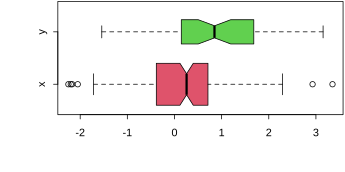
\includegraphics{gallery_files/figure-latex/rnorm-boxplot-1} 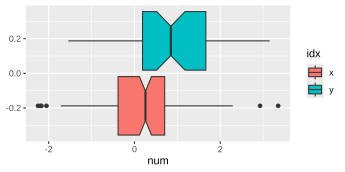
\includegraphics{gallery_files/figure-latex/rnorm-boxplot-2} 

}

\caption[箱线图的凹槽与统计推断]{箱线图的凹槽与统计推断:从凹槽不交叠的情况来看,两样本中位数有显著差异。}\label{fig:rnorm-boxplot}
\end{figure}

最后我们再以一个模拟数据的例子展示箱线图凹槽的功能。这里我们分别从正态分布 \(\mathrm{N}(0,1)\) 和 \(\mathrm{N}(0.5,1)\) 中各自产生 150 和 50 个随机数,然后作箱线图比较两组数据中间位置的差异。图 \ref{fig:rnorm-boxplot} 为一次模拟的结果,图中的凹槽表明了两组数据的中位数有显著差异,Wilcoxon 秩和检验也证实了这一结论。此外,该图还使用了 \texttt{varwidth} 参数以表明两组数据样本量的大小不同。

\section{条形图}\label{sec:barplot}





\begin{Shaded}
\begin{Highlighting}[]
\FunctionTok{library}\NormalTok{(RColorBrewer) }\CommentTok{\# 用分类调色板}
\FunctionTok{par}\NormalTok{(}\AttributeTok{mfrow =} \FunctionTok{c}\NormalTok{(}\DecValTok{2}\NormalTok{, }\DecValTok{1}\NormalTok{), }\AttributeTok{mar =} \FunctionTok{c}\NormalTok{(}\DecValTok{3}\NormalTok{, }\FloatTok{2.5}\NormalTok{, }\FloatTok{0.5}\NormalTok{, }\FloatTok{0.1}\NormalTok{))}
\NormalTok{death }\OtherTok{\textless{}{-}} \FunctionTok{t}\NormalTok{(VADeaths)[, }\DecValTok{5}\SpecialCharTok{:}\DecValTok{1}\NormalTok{]}
\FunctionTok{barplot}\NormalTok{(death, }\AttributeTok{col =} \FunctionTok{brewer.pal}\NormalTok{(}\DecValTok{4}\NormalTok{, }\StringTok{"Set1"}\NormalTok{))}
\FunctionTok{barplot}\NormalTok{(death,}
  \AttributeTok{col =} \FunctionTok{brewer.pal}\NormalTok{(}\DecValTok{4}\NormalTok{, }\StringTok{"Set1"}\NormalTok{), }\AttributeTok{beside =} \ConstantTok{TRUE}\NormalTok{,}
  \AttributeTok{legend.text =} \ConstantTok{TRUE}
\NormalTok{)}
\CommentTok{\# ggplot2}
\NormalTok{reshape\_VADeaths }\OtherTok{\textless{}{-}} \FunctionTok{transform}\NormalTok{(}
  \FunctionTok{expand.grid}\NormalTok{(}
    \AttributeTok{sex =} \FunctionTok{colnames}\NormalTok{(VADeaths),}
    \AttributeTok{age =} \FunctionTok{rownames}\NormalTok{(VADeaths)}
\NormalTok{  ),}
  \AttributeTok{rates =} \FunctionTok{as.vector}\NormalTok{(}\FunctionTok{t}\NormalTok{(VADeaths))}
\NormalTok{)}
\NormalTok{p }\OtherTok{\textless{}{-}} \FunctionTok{ggplot}\NormalTok{(}\AttributeTok{data =}\NormalTok{ reshape\_VADeaths, }\FunctionTok{aes}\NormalTok{(}\AttributeTok{x =}\NormalTok{ age, }\AttributeTok{y =}\NormalTok{ rates, }\AttributeTok{fill =}\NormalTok{ sex))}
\NormalTok{p1 }\OtherTok{\textless{}{-}}\NormalTok{ p }\SpecialCharTok{+} \FunctionTok{geom\_col}\NormalTok{(}\AttributeTok{position =} \StringTok{"stack"}\NormalTok{)}
\NormalTok{p2 }\OtherTok{\textless{}{-}}\NormalTok{ p }\SpecialCharTok{+} \FunctionTok{geom\_col}\NormalTok{(}\AttributeTok{position =} \StringTok{"dodge"}\NormalTok{)}
\FunctionTok{plot\_grid}\NormalTok{(p1, p2, }\AttributeTok{ncol =} \DecValTok{1}\NormalTok{)}
\end{Highlighting}
\end{Shaded}

\begin{figure}

{\centering 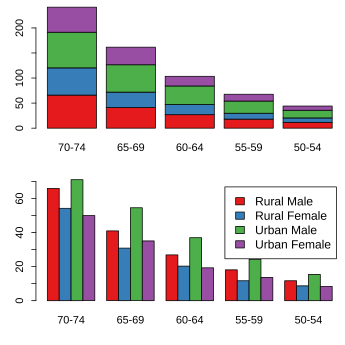
\includegraphics{gallery_files/figure-latex/vadeaths-barplot-1} 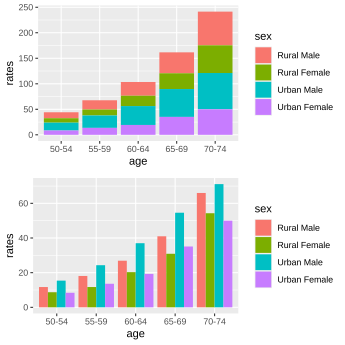
\includegraphics{gallery_files/figure-latex/vadeaths-barplot-2} 

}

\caption[弗吉尼亚死亡率数据条形图]{弗吉尼亚死亡率数据条形图: 堆砌和并列的条形图效果}\label{fig:vadeaths-barplot}
\end{figure}

如同前面 \ref{sec:begin} 节中曾经提到的,条形图目前是各种统计图形中应用最广泛的,但条形图所能展示的统计量比较贫乏:它只能以矩形条的长度展示原始数值,对数据没有任何概括或推断。

R 中条形图的函数为 \texttt{barplot()},用法如下:

\begin{Shaded}
\begin{Highlighting}[]
\FunctionTok{usage}\NormalTok{(barplot.default)}
\end{Highlighting}
\end{Shaded}

\begin{verbatim}
## ## Default S3 method:
## barplot(height, width = 1, space = NULL, names.arg = NULL, legend.text = NULL,
##   beside = FALSE, horiz = FALSE, density = NULL, angle = 45, col = NULL,
##   border = par("fg"), main = NULL, sub = NULL, xlab = NULL, ylab = NULL,
##   xlim = NULL, ylim = NULL, xpd = TRUE, log = "", axes = TRUE,
##   axisnames = TRUE, cex.axis = par("cex.axis"), cex.names = par("cex.axis"),
##   inside = TRUE, plot = TRUE, axis.lty = 0, offset = 0, add = FALSE,
##   ann = !add && par("ann"), args.legend = NULL, ...)
\end{verbatim}

条形图的主要参数是 \texttt{height},它指定了长条的长度,这个参数可以接受一个数值向量或者一个数值矩阵作为参数,前者容易理解,后者稍有些复杂,当传入一个矩阵时,条形图针对矩阵的每一列画图,若 \texttt{beside} 为 \texttt{FALSE},则矩阵每一列占据一条的位置,该条由若干矩形堆砌而成,这些矩形的高度对应着矩阵的行数据,若 \texttt{beside} 为 \texttt{TRUE},这些矩形则并排排列而非堆砌; \texttt{width} 可以设置条的宽度; \texttt{space} 用以设置条之间的间距; \texttt{names.arg} 为条形图的标签,即每一条的名称; \texttt{legend.text} 参数在 \texttt{height} 为矩阵时比较有用,可以用来添加图例; \texttt{horiz} 用以设置条形图的方向(水平或垂直); \texttt{density} 、 \texttt{angle} 等参数可以参考矩形的章节(\ref{sec:polygon} 节); \texttt{plot} 为逻辑值,决定是否将条形图添加到现有图形上。

图 \ref{fig:vadeaths-barplot}
下图展示了参数 \texttt{beside} 和 \texttt{legend.text} 的效果。该图以 1940 年弗吉尼亚州分年龄组、分地区和分性别死亡率数据 \texttt{VADeaths} 为基础,展示了各组之间死亡率的差异,其中堆砌的条形图容易比较各年龄组总死亡率的大小,显然年龄越高死亡率越大,而并列的条形图容易比较组内的城乡和性别差异,一般说来,男性死亡率高于女性,农村男性死亡率低于城市男性,但女性的城乡差异没有明显规律。由于人眼对长度比比例更敏感(例如在区分城乡和性别差异时,图 \ref{fig:vadeaths-barplot}
的上图就不如下图直观),所以我们制图时要考虑清楚我们想展示的是数据的哪一方面,即:将最关键的信息用最能激发视觉感知的形式表现出来。

\begin{Shaded}
\begin{Highlighting}[]
\NormalTok{VADeaths }\CommentTok{\# 弗吉尼亚州死亡数据}
\end{Highlighting}
\end{Shaded}

\begin{verbatim}
##       Rural Male Rural Female Urban Male Urban Female
## 50-54       11.7          8.7       15.4          8.4
## 55-59       18.1         11.7       24.3         13.6
## 60-64       26.9         20.3       37.0         19.3
## 65-69       41.0         30.9       54.6         35.1
## 70-74       66.0         54.3       71.1         50.0
\end{verbatim}

\section{散点图}\label{sec:plot-default}

散点图通常用来展示两个变量之间的关系,这种关系可能是线性或非线性的。图中每一个点的横纵坐标都分别对应两个变量各自的观测值,因此散点所反映出来的趋势也就是两个变量之间的关系。

R 中散点图的函数为 \texttt{plot.default()},但由于 \texttt{plot()} 是泛型函数(参见 \ref{sec:plot} 小节),通常我们只需要提供两个数值型向量给 \texttt{plot()} 即可画散点图,或者提供一个两列的矩阵或数据框。函数 \texttt{plot.default()} 的用法如下:

\begin{Shaded}
\begin{Highlighting}[]
\FunctionTok{usage}\NormalTok{(plot.default)}
\end{Highlighting}
\end{Shaded}

\begin{verbatim}
## ## Default S3 method:
## plot(x, y = NULL, type = "p", xlim = NULL, ylim = NULL, log = "", main = NULL,
##   sub = NULL, xlab = NULL, ylab = NULL, ann = par("ann"), axes = TRUE,
##   frame.plot = axes, panel.first = NULL, panel.last = NULL, asp = NA,
##   xgap.axis = NA, ygap.axis = NA, ...)
\end{verbatim}

其中若 \texttt{x} 是一个两列的矩阵或数据框,则无需再提供 \texttt{y} ,否则 \texttt{x} 和 \texttt{y} 都必须是数值型向量;其它参数均已在 \ref{sec:plot} 小节中介绍。





\begin{Shaded}
\begin{Highlighting}[]
\FunctionTok{demo}\NormalTok{(}\StringTok{"alphaDemo"}\NormalTok{, }\AttributeTok{package =} \StringTok{"MSG"}\NormalTok{)}

\NormalTok{p }\OtherTok{\textless{}{-}} \FunctionTok{ggplot}\NormalTok{(BinormCircle, }\FunctionTok{aes}\NormalTok{(V1, V2)) }\SpecialCharTok{+}
  \FunctionTok{theme\_void}\NormalTok{() }\SpecialCharTok{+}
  \FunctionTok{theme}\NormalTok{(}\AttributeTok{axis.ticks =} \FunctionTok{element\_blank}\NormalTok{(), }
    \AttributeTok{axis.text =} \FunctionTok{element\_blank}\NormalTok{(),}
    \AttributeTok{axis.title =} \FunctionTok{element\_blank}\NormalTok{(),}
    \AttributeTok{plot.background =} \FunctionTok{element\_rect}\NormalTok{(}\AttributeTok{linetype =} \StringTok{"solid"}\NormalTok{,}\AttributeTok{color =} \StringTok{"black"}\NormalTok{)}
\NormalTok{  )}
\NormalTok{p1 }\OtherTok{\textless{}{-}}\NormalTok{ p }\SpecialCharTok{+} \FunctionTok{geom\_point}\NormalTok{(}\AttributeTok{color =} \FunctionTok{rgb}\NormalTok{(}\DecValTok{1}\NormalTok{, }\DecValTok{0}\NormalTok{, }\DecValTok{0}\NormalTok{))}
\NormalTok{p2 }\OtherTok{\textless{}{-}}\NormalTok{ p }\SpecialCharTok{+} \FunctionTok{geom\_point}\NormalTok{(}\AttributeTok{color =} \FunctionTok{rgb}\NormalTok{(}\DecValTok{1}\NormalTok{, }\DecValTok{0}\NormalTok{, }\DecValTok{0}\NormalTok{), }\AttributeTok{alpha =} \FloatTok{0.01}\NormalTok{)}
\FunctionTok{plot\_grid}\NormalTok{(p1, p2, }\AttributeTok{ncol =} \DecValTok{2}\NormalTok{)}
\end{Highlighting}
\end{Shaded}

\begin{figure}

{\centering 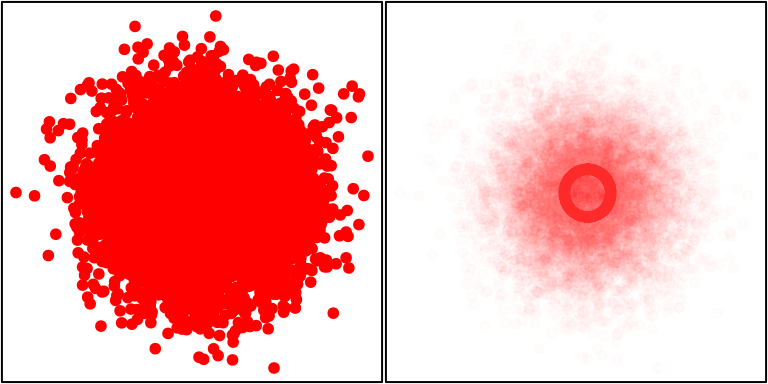
\includegraphics{gallery_files/figure-latex/scatter-alpha-1} 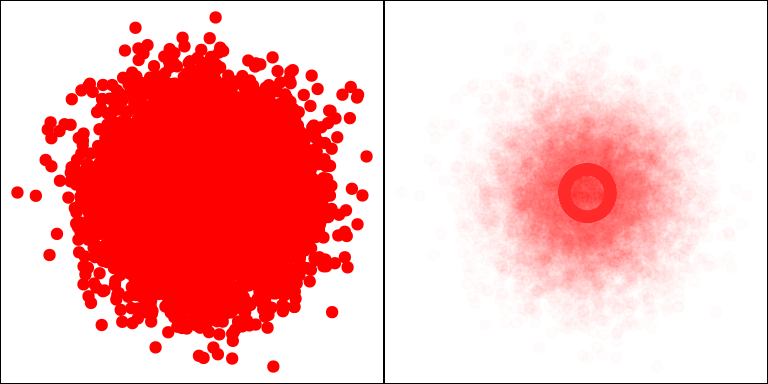
\includegraphics{gallery_files/figure-latex/scatter-alpha-2} 

}

\caption[半透明散点图中的规律]{半透明散点图中的规律:左图是一幅普通的散点图,图中几乎看不出数据有任何异常特征;右图中对点使用了透明度为 0.01 的红色,图中立即显示出一个深色的圆圈,表明该圆圈上集中了大量数据点。}\label{fig:scatter-alpha}
\end{figure}

图 \ref{fig:scatter-alpha}
展示了一个人造数据的散点图:我们设计了 2 万个样本,其中有 1 万个样本点来自于两个独立的标准正态分布,另 1 万个样本点的坐标落在半径为 0.5 的圆上,最后将这 2 万个样本拼起来并打乱顺序。该数据收录在 \textbf{MSG} 包中,名为 \texttt{BinormCircle}。虽然数据只有两个变量,但我们用普通的统计模型和数值分析几乎无法找出数据的特征,例如线性回归显示两个变量 \texttt{V1} 和 \texttt{V2} 的回归系数非常不显著:

\begin{Shaded}
\begin{Highlighting}[]
\FunctionTok{data}\NormalTok{(BinormCircle, }\AttributeTok{package =} \StringTok{"MSG"}\NormalTok{)}
\FunctionTok{head}\NormalTok{(BinormCircle) }\CommentTok{\# 数据前 6 行}
\end{Highlighting}
\end{Shaded}

\begin{verbatim}
##       V1     V2
## 1  0.889 -1.764
## 2  0.072 -0.495
## 3  0.123 -0.180
## 4 -0.499  0.030
## 5  0.252  0.432
## 6  0.450  0.218
\end{verbatim}

\begin{Shaded}
\begin{Highlighting}[]
\CommentTok{\# 回归系数以及 P 值(不显著)}
\FunctionTok{coef}\NormalTok{(}\FunctionTok{summary}\NormalTok{(}\FunctionTok{lm}\NormalTok{(V2 }\SpecialCharTok{\textasciitilde{}}\NormalTok{ V1, BinormCircle)))}
\end{Highlighting}
\end{Shaded}

\begin{verbatim}
##                 Estimate  Std. Error    t value  Pr(>|t|)
## (Intercept) -0.006085156 0.005258164 -1.1572776 0.2471728
## V1           0.003988851 0.007015317  0.5685917 0.5696397
\end{verbatim}

换用高阶回归的结果也类似,无论回归阶数为多少,系数均不显著,这一点从数据的构造上就可以知道(理论上两个变量的相关系数为 0)。由于样本量太大,普通的散点图上点与点之间严重重叠,所以也很难看出散点图有何异常,而使用半透明色的散点图则很容易看出,在大量的数据点中,还隐藏着一个圆圈,说明有相当一部分数据分布有特殊规律。我们在网页 \url{https://yihui.org/en/2008/09/to-see-a-circle-in-a-pile-of-sand/}
上给出了其它五种不同的解决方案,都可以从图形的角度反映出这种规律。本章 \ref{sec:smoothScatter} 小节也将以平滑散点图的方式再回顾这批数据。

\section{关联图}\label{sec:assocplot}





\begin{Shaded}
\begin{Highlighting}[]
\NormalTok{(x }\OtherTok{\textless{}{-}} \FunctionTok{margin.table}\NormalTok{(HairEyeColor, }\FunctionTok{c}\NormalTok{(}\DecValTok{1}\NormalTok{, }\DecValTok{2}\NormalTok{)))}
\end{Highlighting}
\end{Shaded}

\begin{verbatim}
##        Eye
## Hair    Brown Blue Hazel Green
##   Black    68   20    15     5
##   Brown   119   84    54    29
##   Red      26   17    14    14
##   Blond     7   94    10    16
\end{verbatim}

\begin{Shaded}
\begin{Highlighting}[]
\FunctionTok{assocplot}\NormalTok{(x)}
\end{Highlighting}
\end{Shaded}

\begin{figure}

{\centering 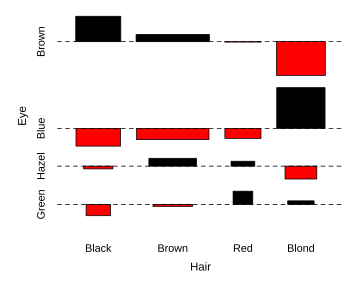
\includegraphics{gallery_files/figure-latex/assocplot-1} 

}

\caption[眼睛颜色与头发颜色的关联图]{眼睛颜色与头发颜色的关联图}\label{fig:assocplot}
\end{figure}

\begin{Shaded}
\begin{Highlighting}[]
\FunctionTok{chisq.test}\NormalTok{(x)}\SpecialCharTok{$}\NormalTok{p.value }\CommentTok{\# 卡方检验 P 值}
\end{Highlighting}
\end{Shaded}

\begin{verbatim}
## [1] 2.325287e-25
\end{verbatim}

关联图(Cohen-Friendly Association
Plot)是展示二维列联表数据的一种工具 \citep{Cohen80, Friendly92},它主要是基于列联表的独立性检验理论(Pearson
\(\chi^{2}\) 检验)生成的图形。

我们知道,对于一个 \(r\times c\) 列联表,\(\chi^{2}\) 统计量的定义为如下平方和形式:

\begin{equation} 
\chi^{2}=\sum_{i=1}^{r}\sum_{j=1}^{c}d_{ij}^{2};\;\; d_{ij}=\frac{f_{ij}-e_{ij}}{\sqrt{e_{ij}}}
\label{eq:cap}
\end{equation}

其中,\(f_{ij}\) 为单元格中的观测频数,\(e_{ij}\) 为期望频数,二者相差越大,则会导致检验统计量的值越大,说明行变量和列变量越不独立。关联图所展示内容的正是这种差异,它的设计思路是,将图形同样以 \(r\times c\) 的形式布局,每一个 ``单元格'' 中用一个矩形表示观测频数和期望频数的信息,具体来说,矩形的高度与 Pearson 残差 \(f_{ij}-e_{ij}\) 成比例,宽度与期望频数 \(\sqrt{e_{ij}}\) 成比例,这样一来,矩形的面积便与 \(d_{ij}\) 成比例;此外,矩形自身带有方向,朝上表示残差为正,朝下则为负,不同方向的矩形同时也以不同颜色区分开来。

R 中关联图的函数为 \texttt{assocplot()},用法如下:

\begin{Shaded}
\begin{Highlighting}[]
\FunctionTok{usage}\NormalTok{(assocplot)}
\end{Highlighting}
\end{Shaded}

\begin{verbatim}
## assocplot(x, col = c("black", "red"), space = 0.3, main = NULL, xlab = NULL,
##   ylab = NULL)
\end{verbatim}

其中 \texttt{x} 为一个列联表数据(或者矩阵); \texttt{col} 为朝上和朝下矩形的颜色; \texttt{space} 用来设置矩形之间的间距。

图 \ref{fig:assocplot}
是关于 \texttt{HairEyeColor} 数据的关联图。原始数据为一个三维数组,首先我们在性别维度上将数据汇总,得到眼睛颜色(棕蓝褐绿)和头发颜色(黑棕红金)人数的列联表。我们关心的问题是头发颜色与眼睛颜色之间是否存在关联,当然我们可以马上用函数 \texttt{chisq.test()} 作检验,但是检验的结果非常单一,我们只能知道零假设(独立)可否被拒绝,而图 \ref{fig:assocplot} 则细致展示了数据的内部信息,例如从图中我们可以清楚看到,并非所有单元格都与期望频数有很大差异,只是少数几个单元格贡献了较大的 \(\chi^{2}\) 值,如金发碧眼、金发棕眼等;事实上,这批数据为调查数据,眼睛颜色和头发颜色都为受访者(Delaware 大学的 592 名学生)自己填写,我们观察到金发碧眼单元格的期望频数和实际频数差异甚大,据说这背后有一则有趣的故事:由于``金发碧眼''是大家公认的美的标准,因此有些学生在填问卷时故意偏向于填写``金发碧眼'',导致``金发碧眼''的实际频数严重偏高\footnote{本书作者在爱荷华州立大学统计系读博士期间,每周统计图形小组有一次讨论,这则消息来自于作者的一位导师 Heike Hofmann 教授}。从图 \ref{fig:assocplot} 的代码输出中我们知道,\(\chi^{2}\) 检验可以拒绝零假设,眼睛的颜色与头发的颜色并不独立,二者之间存在某种关联关系,然而这种关联关系是由于生物或遗传原因引起还是受访者有意隐瞒自己的信息,则需要我们进一步斟酌了。

在 \textbf{vcd} 包 \citep{vcd} 中有一个类似的关联图函数 \texttt{assoc()},但功能比本节中介绍的函数要更强大,详细介绍参见 \citeauthor{Meyer06} \citetext{\citeyear{Meyer06}; \citealp{Zeileis07}}。

\section{条件密度图}\label{sec:cdplot}

条件密度图(Conditional Density Plot),顾名思义,展示的是一个变量的条件密度,确切的说是一个分类变量 \(Y\) 相对一个连续变量 \(X\) 的条件密度 \(P(Y|X)\)。假设 \(Y\) 的取值为 \(1,2,\cdots,k\),那么条件密度图将按照 \(X\) 的取值从小到大在纵轴方向上依次展示出 \(Y=i\;(i=1,2,\cdots,k)\) 的条件概率分布比例 \(P_{i}=P(Y=i|X=x)\),这些比例大小沿横轴方向上以多边形表示,在任一一个 \(X\) 点,所有比例之和均为 1,这个性质是显而易见的:

\begin{equation} 
\sum_{i=1}^{k}P(Y=i|X=x)=1;\;\forall x
\label{eq:cdp}
\end{equation}

R 中条件密度图的函数为 \texttt{cdplot()},它主要是基于密度函数 \texttt{density()} 完成条件密度的计算 \citep{Hofmann05},其用法如下:

\begin{Shaded}
\begin{Highlighting}[]
\FunctionTok{usage}\NormalTok{(graphics}\SpecialCharTok{:::}\NormalTok{cdplot.default)}
\end{Highlighting}
\end{Shaded}

\begin{verbatim}
## ## Default S3 method:
## cdplot(x, y, plot = TRUE, tol.ylab = 0.05, ylevels = NULL, bw = "nrd0",
##   n = 512, from = NULL, to = NULL, col = NULL, border = 1, main = "",
##   xlab = NULL, ylab = NULL, yaxlabels = NULL, xlim = NULL, ylim = c(0, 1),
##   weights = NULL, ...)
\end{verbatim}

\begin{Shaded}
\begin{Highlighting}[]
\FunctionTok{usage}\NormalTok{(graphics}\SpecialCharTok{:::}\NormalTok{cdplot.formula)}
\end{Highlighting}
\end{Shaded}

\begin{verbatim}
## ## S3 method for class 'formula'
## cdplot(formula, data = list(), plot = TRUE, tol.ylab = 0.05, ylevels = NULL,
##   bw = "nrd0", n = 512, from = NULL, to = NULL, col = NULL, border = 1,
##   main = "", xlab = NULL, ylab = NULL, yaxlabels = NULL, xlim = NULL,
##   ylim = c(0, 1), ..., subset = NULL, weights = NULL)
\end{verbatim}

函数 \texttt{cdplot()} 是泛型函数,它可以支持两种参数类型:直接输入两个数值向量 \texttt{x} 和 \texttt{y} 或者一个公式 \texttt{y\textasciitilde{}x}。 \texttt{x} 为条件变量 \(X\),它是一个数值向量, \texttt{y} 是一个因子向量,即离散变量 \(Y\); \texttt{plot} 为逻辑值,决定了是否作出图形(或者仅仅是计算而不作图); \texttt{ylevels} 给出因子的取值水平(或者分类的名称), \texttt{bw} 、 \texttt{n} 、 \texttt{from} 和 \texttt{to} 都将被传递给 \texttt{density()} 函数以计算密度值,请参考 \texttt{density()} 帮助文件; \texttt{col} 给定一个颜色向量用以代表 \(Y\) 的各种取值(默认为不同深浅的灰色); \texttt{border} 为多边形的边线颜色;其它参数诸如标题、坐标轴范围等此处略去。





\begin{Shaded}
\begin{Highlighting}[]
\FunctionTok{demo}\NormalTok{(}\StringTok{"cdplotDemo"}\NormalTok{, }\AttributeTok{package =} \StringTok{"MSG"}\NormalTok{)}

\NormalTok{fail }\OtherTok{\textless{}{-}}  \FunctionTok{factor}\NormalTok{(}
  \FunctionTok{c}\NormalTok{(}\DecValTok{2}\NormalTok{, }\DecValTok{2}\NormalTok{, }\DecValTok{2}\NormalTok{, }\DecValTok{2}\NormalTok{, }\DecValTok{1}\NormalTok{, }\DecValTok{1}\NormalTok{, }\DecValTok{1}\NormalTok{, }\DecValTok{1}\NormalTok{, }\DecValTok{1}\NormalTok{, }\DecValTok{1}\NormalTok{, }\DecValTok{2}\NormalTok{, }\DecValTok{1}\NormalTok{,}
    \DecValTok{2}\NormalTok{, }\DecValTok{1}\NormalTok{, }\DecValTok{1}\NormalTok{, }\DecValTok{1}\NormalTok{, }\DecValTok{1}\NormalTok{, }\DecValTok{2}\NormalTok{, }\DecValTok{1}\NormalTok{, }\DecValTok{1}\NormalTok{, }\DecValTok{1}\NormalTok{, }\DecValTok{1}\NormalTok{, }\DecValTok{1}\NormalTok{),}
  \AttributeTok{levels =} \DecValTok{2}\SpecialCharTok{:}\DecValTok{1}\NormalTok{, }
  \AttributeTok{labels =} \FunctionTok{c}\NormalTok{(}\StringTok{"yes"}\NormalTok{, }\StringTok{"no"}\NormalTok{)}
\NormalTok{)}
\NormalTok{temperature }\OtherTok{=} \FunctionTok{c}\NormalTok{(}\DecValTok{53}\NormalTok{, }\DecValTok{57}\NormalTok{, }\DecValTok{58}\NormalTok{, }\DecValTok{63}\NormalTok{, }\DecValTok{66}\NormalTok{, }\DecValTok{67}\NormalTok{, }\DecValTok{67}\NormalTok{, }\DecValTok{67}\NormalTok{, }\DecValTok{68}\NormalTok{, }\DecValTok{69}\NormalTok{, }\DecValTok{70}\NormalTok{,}
  \DecValTok{70}\NormalTok{, }\DecValTok{70}\NormalTok{, }\DecValTok{70}\NormalTok{, }\DecValTok{72}\NormalTok{, }\DecValTok{73}\NormalTok{, }\DecValTok{75}\NormalTok{, }\DecValTok{75}\NormalTok{, }\DecValTok{76}\NormalTok{, }\DecValTok{76}\NormalTok{, }\DecValTok{78}\NormalTok{, }\DecValTok{79}\NormalTok{, }\DecValTok{81}
\NormalTok{)}
\NormalTok{fail\_temperature }\OtherTok{\textless{}{-}} \FunctionTok{data.frame}\NormalTok{(}\AttributeTok{fail =}\NormalTok{ fail, }\AttributeTok{temperature =}\NormalTok{ temperature)}
\FunctionTok{ggplot}\NormalTok{(fail\_temperature, }\FunctionTok{aes}\NormalTok{(temperature, }\FunctionTok{after\_stat}\NormalTok{(count), }\AttributeTok{fill =}\NormalTok{ fail)) }\SpecialCharTok{+}
  \FunctionTok{geom\_density}\NormalTok{(}\AttributeTok{position =} \StringTok{"fill"}\NormalTok{) }\SpecialCharTok{+}
  \FunctionTok{geom\_point}\NormalTok{(}\FunctionTok{aes}\NormalTok{(temperature, }\FunctionTok{c}\NormalTok{(}\FloatTok{0.75}\NormalTok{, }\FloatTok{0.25}\NormalTok{)[}\FunctionTok{as.integer}\NormalTok{(fail)]),}
    \AttributeTok{shape =} \DecValTok{21}\NormalTok{, }\AttributeTok{colour =} \StringTok{"blue"}\NormalTok{, }\AttributeTok{fill =} \StringTok{"yellow"}\NormalTok{) }\SpecialCharTok{+}
  \FunctionTok{scale\_x\_continuous}\NormalTok{(}\AttributeTok{expand =} \FunctionTok{c}\NormalTok{(}\DecValTok{0}\NormalTok{, }\DecValTok{0}\NormalTok{)) }\SpecialCharTok{+}
  \FunctionTok{scale\_y\_continuous}\NormalTok{(}\StringTok{"fail"}\NormalTok{, }\AttributeTok{expand =} \FunctionTok{c}\NormalTok{(}\DecValTok{0}\NormalTok{, }\DecValTok{0}\NormalTok{), }\AttributeTok{breaks =} \FunctionTok{c}\NormalTok{(}\FloatTok{0.25}\NormalTok{, }\FloatTok{0.75}\NormalTok{), }
    \AttributeTok{labels =} \FunctionTok{c}\NormalTok{(}\StringTok{"no"}\NormalTok{, }\StringTok{"yes"}\NormalTok{),}
    \AttributeTok{sec.axis =} \FunctionTok{dup\_axis}\NormalTok{(}\AttributeTok{name =} \ConstantTok{NULL}\NormalTok{, }
      \AttributeTok{breaks =} \FunctionTok{seq}\NormalTok{(}\DecValTok{0}\NormalTok{, }\DecValTok{1}\NormalTok{, }\FloatTok{0.2}\NormalTok{), }
      \AttributeTok{labels =} \FunctionTok{c}\NormalTok{(}\DecValTok{0}\NormalTok{, }\StringTok{""}\NormalTok{, }\FloatTok{0.4}\NormalTok{, }\StringTok{""}\NormalTok{, }\FloatTok{0.8}\NormalTok{, }\StringTok{""}\NormalTok{))}
\NormalTok{  ) }\SpecialCharTok{+}
  \FunctionTok{scale\_fill\_manual}\NormalTok{(}\AttributeTok{values =} \FunctionTok{c}\NormalTok{(}\StringTok{"red"}\NormalTok{, }\StringTok{"lightblue"}\NormalTok{)) }\SpecialCharTok{+}
  \FunctionTok{theme\_classic}\NormalTok{() }\SpecialCharTok{+}
  \FunctionTok{theme}\NormalTok{(}\AttributeTok{legend.position =} \StringTok{"none"}\NormalTok{)}
\end{Highlighting}
\end{Shaded}

\begin{figure}

{\centering 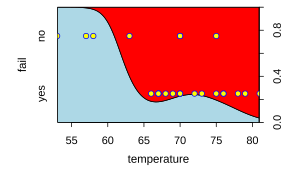
\includegraphics{gallery_files/figure-latex/cdplot-1} 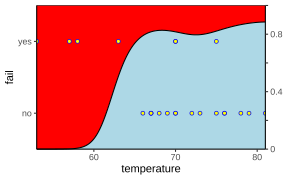
\includegraphics{gallery_files/figure-latex/cdplot-2} 

}

\caption[航天飞机 O 型环在不同温度下失效的条件密度图]{航天飞机 O 型环在不同温度下失效的条件密度图:随着温度升高,O 型环越来越不容易失效。}\label{fig:cdplot}
\end{figure}

这里我们以美国国家航空和宇宙航行局的一批 O 型环(O-ring,一种由橡胶或塑料制成的平环,用作垫圈)失效数据为例,这批数据有两个变量:温度变量和是否失效的变量。为了探索温度对 O 型环失效的影响,我们可以使用诸如 Logistic 回归之类的统计模型去计算、分析,而这里我们用条件密度图来展示温度的影响,如图 \ref{fig:cdplot}。由于因变量是一个二分类变量,图中相应有两个多边形(带颜色的区域)分别表示是否失效,从图中我们可以清楚观察到,随着温度的上升,失效的可能性越来越小(下面的多边形高度越来越高),但失效的概率与温度并不是简单的线性关系,例如 55 到 65 之间的温度上升会使得失效概率迅速下降,而当气温更高的时候,失效概率下降的速度会减缓。为了更清楚地观察条件密度图的效果,我们也将原始数据以点的形式添加到图中;不难发现,O 型环失效的情况大多对应着相对较低的温度。

这里需要提醒读者注意的是,密度值的计算和估计与数据样本量大小有关系,小的样本量可能会导致密度估计的不精确,进而导致图形的误导性,因此使用条件密度图的时候务必注意样本量的问题。

\section{等高图/等高线}\label{sec:contour}

等高图(Contour Plot)和等高线(Contour
Line)表面上看起来是二维形式,但实际上展示的是三维数据。我们知道,三维图形往往比二维图形看起来更具有吸引力,然而在平面上展示三维图形也有其缺陷,最主要的就是视角问题,一幅三维图形可以有无数种视角,正视、侧视、俯视可能都会看到不同的信息,而且各种角度下可能都有一部分数据被前面的数据挡住而不能被看到,当然这些问题都可以通过更灵活的图形设备克服,如 \textbf{rgl} 包 \citep{rgl},但是在更多的情况下,我们的图形都必须展示在静态介质上(如书籍、论文等),我们不可能在纸面上拖动鼠标对图形进行交互式操作,因此,我们需要等高图这样一种以二维形式展示三维数据的工具。





\begin{figure}

{\centering 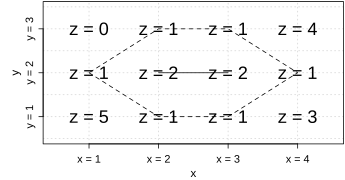
\includegraphics{gallery_files/figure-latex/contour-grid-1} 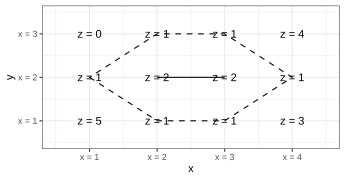
\includegraphics{gallery_files/figure-latex/contour-grid-2} 

}

\caption[网格数据的示意图]{网格数据的示意图:体会 x、y 与 z 的对应关系}\label{fig:contour-grid}
\end{figure}

首先我们需要理解等高图所展示数据的形式,因为它与我们想象的三维数据有所不同:并非三个数值向量,而是两个数值向量 x、y 和一个相应的矩阵 z。我们不妨将数据的形式想象为一座山峰,两个数值向量分别是横向和纵向的位置(如经纬度),第三维数据是每一种横纵向位置点组合上的高度,而横纵交叉组合之后形成的是一个网格,矩阵 z 则是这个网格上的高度数值,用数学式子表示这种关系就是 \(z_{ij}=f(x_{i},y_{j})\)。图 \ref{fig:contour-grid} 为这种网格数据的示意图,请读者自行体会。

所谓等高线,就是将平面上对应的 z 值(高度)相等的点连接起来形成的线。同样,我们可以以一座山峰来想象:在同一海拔高度上围绕山峰一圈的线就是一条等高线。图 \ref{fig:contour-grid}
中的连线即等高线,如实线表示的是高度为 2 的点,而虚线表示高度为 1 的点。注意等高线之间不可能相交,因为同一点不可能同时有两种高度。

等高线上通常会有数字表示高度,从这些数字我们不难想象出三维的山峰的形状,从这个意义上来说,等高图本质上也是一种三维图示方法。

R 中等高图的函数为 \texttt{contour()},同时 \textbf{grDevices} 包中也提供了等高线的计算函数 \texttt{contourLines()},用法分别如下:

\begin{Shaded}
\begin{Highlighting}[]
\FunctionTok{usage}\NormalTok{(contour.default)}
\end{Highlighting}
\end{Shaded}

\begin{verbatim}
## ## Default S3 method:
## contour(x = seq(0, 1, length.out = nrow(z)),
##   y = seq(0, 1, length.out = ncol(z)), z, nlevels = 10,
##   levels = pretty(zlim, nlevels), labels = NULL,
##   xlim = range(x, finite = TRUE), ylim = range(y, finite = TRUE),
##   zlim = range(z, finite = TRUE), labcex = 0.6, drawlabels = TRUE,
##   method = "flattest", vfont, axes = TRUE, frame.plot = axes, col = par("fg"),
##   lty = par("lty"), lwd = par("lwd"), add = FALSE, ...)
\end{verbatim}

\begin{Shaded}
\begin{Highlighting}[]
\FunctionTok{usage}\NormalTok{(contourLines)}
\end{Highlighting}
\end{Shaded}

\begin{verbatim}
## contourLines(x = seq(0, 1, length.out = nrow(z)),
##   y = seq(0, 1, length.out = ncol(z)), z, nlevels = 10,
##   levels = pretty(range(z, na.rm = TRUE), nlevels))
\end{verbatim}

参数 \texttt{x} 、 \texttt{y} 与 \texttt{z} 此处不再介绍; \texttt{nlevels} 可以设定等高线的条数、调整等高线的疏密; \texttt{levels} 设定一系列等高线的 \texttt{z} 值,只有这些值或者这些值附近的点才会被连起来; \texttt{labels} 为等高线上的标记字符串,默认是高度的数值; \texttt{xlim} 、 \texttt{ylim} 和 \texttt{zlim} 设定分别设定 \texttt{x} 、 \texttt{y} 与 \texttt{z} 的范围,默认从数据中获得; \texttt{method} 设定等高线的画法,有三种取值:\texttt{\textquotesingle{}simple\textquotesingle{}}(在等高线的末端加标签、标签与等高线重叠)、\texttt{\textquotesingle{}edge\textquotesingle{}}(在等高线的末端加标签、标签嵌在等高线内)或 \texttt{\textquotesingle{}flattest\textquotesingle{}}(在等高线最平缓的地方加标签、嵌在等高线内);其它参数用来调整等高图的外观,此处略去不介绍。





\begin{Shaded}
\begin{Highlighting}[]
\FunctionTok{par}\NormalTok{(}\AttributeTok{mar =} \FunctionTok{c}\NormalTok{(}\DecValTok{4}\NormalTok{, }\DecValTok{4}\NormalTok{, }\FloatTok{0.2}\NormalTok{, }\FloatTok{0.2}\NormalTok{))}
\FunctionTok{library}\NormalTok{(MSG)}
\FunctionTok{data}\NormalTok{(ChinaLifeEdu)}
\NormalTok{x }\OtherTok{\textless{}{-}}\NormalTok{ ChinaLifeEdu}
\FunctionTok{library}\NormalTok{(KernSmooth)}
\end{Highlighting}
\end{Shaded}

\begin{verbatim}
## KernSmooth 2.23 loaded
## Copyright M. P. Wand 1997-2009
\end{verbatim}

\begin{Shaded}
\begin{Highlighting}[]
\NormalTok{est }\OtherTok{\textless{}{-}} \FunctionTok{bkde2D}\NormalTok{(x, }\FunctionTok{apply}\NormalTok{(x, }\DecValTok{2}\NormalTok{, dpik))}
\FunctionTok{contour}\NormalTok{(est}\SpecialCharTok{$}\NormalTok{x1, est}\SpecialCharTok{$}\NormalTok{x2, est}\SpecialCharTok{$}\NormalTok{fhat,}
  \AttributeTok{nlevels =} \DecValTok{15}\NormalTok{, }\AttributeTok{col =} \StringTok{"darkgreen"}\NormalTok{,}
  \AttributeTok{vfont =} \FunctionTok{c}\NormalTok{(}\StringTok{"sans serif"}\NormalTok{, }\StringTok{"plain"}\NormalTok{),}
  \AttributeTok{xlab =} \StringTok{"预期寿命"}\NormalTok{,}
  \AttributeTok{ylab =} \StringTok{"高学历人数"}
\NormalTok{)}
\FunctionTok{points}\NormalTok{(x, }\AttributeTok{pch =} \DecValTok{20}\NormalTok{)}


\NormalTok{est\_tidy }\OtherTok{\textless{}{-}} \FunctionTok{data.frame}\NormalTok{(}
  \AttributeTok{life =} \FunctionTok{rep}\NormalTok{(est}\SpecialCharTok{$}\NormalTok{x1, }\FunctionTok{length}\NormalTok{(est}\SpecialCharTok{$}\NormalTok{x2)),}
  \AttributeTok{edu =} \FunctionTok{rep}\NormalTok{(est}\SpecialCharTok{$}\NormalTok{x2, }\AttributeTok{each =} \FunctionTok{length}\NormalTok{(est}\SpecialCharTok{$}\NormalTok{x1)),}
  \AttributeTok{z =} \FunctionTok{as.vector}\NormalTok{(est}\SpecialCharTok{$}\NormalTok{fhat)}
\NormalTok{)}
\NormalTok{levels }\OtherTok{\textless{}{-}} \FunctionTok{pretty}\NormalTok{(}\FunctionTok{range}\NormalTok{(est\_tidy}\SpecialCharTok{$}\NormalTok{z, }\AttributeTok{finite =} \ConstantTok{TRUE}\NormalTok{), }\DecValTok{15}\NormalTok{)}

\FunctionTok{ggplot}\NormalTok{(est\_tidy, }\FunctionTok{aes}\NormalTok{(life, edu)) }\SpecialCharTok{+}
  \FunctionTok{geom\_contour}\NormalTok{(}\FunctionTok{aes}\NormalTok{(}\AttributeTok{z =}\NormalTok{ z), }\AttributeTok{breaks =}\NormalTok{ levels, }\AttributeTok{colour =} \StringTok{"darkgreen"}\NormalTok{) }\SpecialCharTok{+}
  \FunctionTok{geom\_point}\NormalTok{(}\FunctionTok{aes}\NormalTok{(Life.Expectancy, High.Edu.NO), }\AttributeTok{data =}\NormalTok{ x) }\SpecialCharTok{+}
  \FunctionTok{labs}\NormalTok{(}\AttributeTok{x =}\StringTok{"预期寿命"}\NormalTok{, }\AttributeTok{y =} \StringTok{"高学历人数"}\NormalTok{) }\SpecialCharTok{+}
  \FunctionTok{theme\_bw}\NormalTok{()}
\end{Highlighting}
\end{Shaded}

\begin{figure}

{\centering 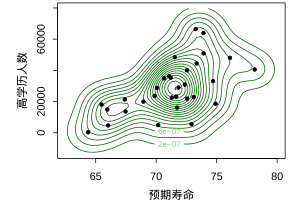
\includegraphics{gallery_files/figure-latex/contour-pop-1} 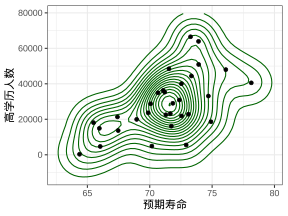
\includegraphics{gallery_files/figure-latex/contour-pop-2} 

}

\caption[中国 31 地区国民预期寿命和高学历人数密度等高图]{2005 年中国 31 地区国民预期寿命和高学历人数密度等高图}\label{fig:contour-pop}
\end{figure}

图 \ref{fig:contour-pop}
利用等高图展示了一个聚类现象。数据来源于 2005 年中国统计年鉴,数值参见 \textbf{MSG} 包中的 \texttt{ChinaLifeEdu} 数据,这里使用了其中两个变量:人口预期寿命(实际数据来自 2000 年)和高学历人口数量(定义为大专以上学历人数)。首先我们对这二维变量利用 \textbf{KernSmooth} 包 \citep{KernSmooth} 进行核密度估计,得到二维核密度值(一个矩阵),然后用两个原始变量以及这个密度值矩阵作等高图。由于密度值反映的是某个位置上数据的密集程度,图 \ref{fig:contour-pop} 所能揭示的现象是:中国 31 省市自治区在人口预期寿命和高学历人口数量上呈现出聚类的特征,图中密度值大的区域主要有中部、右上和左下三个,东中西格局比较明显,即:东部地区分布在图中右上角,中部省市分布在图中中部,西部地区集中在图中的左下角,对照图 \ref{fig:symbols-pop} 可以知道聚类的具体地区名称,就更能理解这里''聚类''的含义了。关于这批数据的分析,我们在 \ref{sec:symbols} 小节仍会继续,这里不再深入。





\begin{Shaded}
\begin{Highlighting}[]
\FunctionTok{par}\NormalTok{(}\AttributeTok{mar =} \FunctionTok{rep}\NormalTok{(}\DecValTok{0}\NormalTok{, }\DecValTok{4}\NormalTok{)) }\CommentTok{\# 继续前面的例子}
\FunctionTok{persp}\NormalTok{(est}\SpecialCharTok{$}\NormalTok{x1, est}\SpecialCharTok{$}\NormalTok{x2, est}\SpecialCharTok{$}\NormalTok{fhat, }\AttributeTok{shade =} \FloatTok{0.75}\NormalTok{, }\AttributeTok{border =} \ConstantTok{NA}\NormalTok{, }
      \AttributeTok{col =} \StringTok{"lightblue"}\NormalTok{, }\AttributeTok{phi =} \DecValTok{20}\NormalTok{, }\AttributeTok{theta =} \DecValTok{15}\NormalTok{, }\AttributeTok{box =} \ConstantTok{FALSE}\NormalTok{)}
\end{Highlighting}
\end{Shaded}

\begin{figure}

{\centering 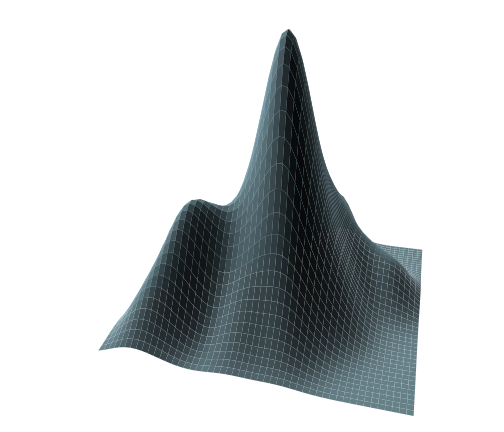
\includegraphics{gallery_files/figure-latex/contour-persp-1} 

}

\caption[与等高图对应的三维透视图]{与等高图对应的三维透视图:从右至左依次有三个山峰,尤其是中部山峰最为突出,对照后面 \ref{sec:symbols} 小节中图 \ref{fig:symbols-pop} 可知,这三个山峰分别代表东中西的省份。}\label{fig:contour-persp}
\end{figure}

在 \textbf{graphics} 包中还有一个类似的等高图函数 \texttt{filled.contour()},它的原理完全类似,只是它用颜色来区分高度值的大小并且有颜色图例,看起来可能更美观一些,\ref{sec:filled-contour} 小节中我们会详细介绍。

\section{条件分割图}\label{sec:coplot}

条件分割图(Conditioning Plot)的思想源自于统计学中的条件分布,即:给定某一个(或几个)变量之后看我们所关心的变量的分布情况。在条件分割图中,这种''分布''主要指的是两个变量之间的关系,通常以散点图表示。

条件分割图可以看作是对散点图的进一步深入发掘,它可以以一个或者两个条件变量作为所有数据的划分条件,条件变量在图形的边缘用灰色矩形条标记出变量的取值范围,每个矩形条对应着一幅散点图(严格来说此时应该称作''条件散点图''),这就是条件分割图的基本做法。后面我们会结合例子详细说明。

R 中条件分割图的函数为 \texttt{coplot()},其用法如下:

\begin{Shaded}
\begin{Highlighting}[]
\FunctionTok{usage}\NormalTok{(coplot)}
\end{Highlighting}
\end{Shaded}

\begin{verbatim}
## coplot(formula, data, given.values, panel = points, rows, columns,
##   show.given = TRUE, col = par("fg"), pch = par("pch"),
##   bar.bg = c(num = gray(0.8), fac = gray(0.95)),
##   xlab = c(x.name, paste("Given :", a.name)),
##   ylab = c(y.name, paste("Given :", b.name)), subscripts = FALSE,
##   axlabels = function(f) abbreviate(levels(f)), number = 6, overlap = 0.5,
##   xlim, ylim, ...)
\end{verbatim}

\begin{Shaded}
\begin{Highlighting}[]
\FunctionTok{usage}\NormalTok{(co.intervals)}
\end{Highlighting}
\end{Shaded}

\begin{verbatim}
## co.intervals(x, number = 6, overlap = 0.5)
\end{verbatim}

参数 \texttt{formula} 为一个公式,形式为 \texttt{y\ \textasciitilde{}\ x\ \textbar{}\ a}(一个条件变量)或 \texttt{y\ \textasciitilde{}\ x\ \textbar{}\ a\ *\ b}(两个条件变量),``\texttt{\textbar{}}'' 后面即为条件变量; \texttt{data} 为数据,其中包含了 \texttt{x} 、 \texttt{y} 、 \texttt{a} 和 \texttt{b} 等变量; \texttt{given.values} 指定条件变量的取值范围; \texttt{panel} 参数为该函数的关键参数,它决定了每一幅散点图的画法,默认只是画点,我们可以将其任意扩展为我们需要的图示功能,如添加回归直线等等; \texttt{rows} 和 \texttt{columns} 参数用来设定散点图的摆放行数和列数; \texttt{col} 和 \texttt{pch} 分别设定散点图中点的颜色和样式; \texttt{bar.bg} 给定条件变量指示条的填充颜色; \texttt{number} 和 \texttt{overlap} 传给 \texttt{co.intervals()} 函数用来计算划分连续变量的区间,前者设定划分段数,后者设定区间之间的重叠比例,如:

\begin{Shaded}
\begin{Highlighting}[]
\FunctionTok{co.intervals}\NormalTok{(}\DecValTok{1}\SpecialCharTok{:}\DecValTok{10}\NormalTok{, }\AttributeTok{number =} \DecValTok{5}\NormalTok{, }\AttributeTok{overlap =} \FloatTok{0.5}\NormalTok{)}
\end{Highlighting}
\end{Shaded}

\begin{verbatim}
##      [,1] [,2]
## [1,]  0.5  3.5
## [2,]  2.5  5.5
## [3,]  3.5  7.5
## [4,]  5.5  8.5
## [5,]  7.5 10.5
\end{verbatim}

上述代码将数字 \texttt{1:10} 划分为了 5 段,每段长度为 2,重叠长度为 1,因此重叠比例为 0.5。条件分割图中散点图的顺序是从左到右、从下到上,分别与条件变量从左到右、从下到上的指示条对应。





\begin{Shaded}
\begin{Highlighting}[]
\FunctionTok{par}\NormalTok{(}\AttributeTok{mar =} \FunctionTok{rep}\NormalTok{(}\DecValTok{0}\NormalTok{, }\DecValTok{4}\NormalTok{), }\AttributeTok{mgp =} \FunctionTok{c}\NormalTok{(}\DecValTok{2}\NormalTok{, .}\DecValTok{5}\NormalTok{, }\DecValTok{0}\NormalTok{))}
\FunctionTok{library}\NormalTok{(maps)}
\FunctionTok{coplot}\NormalTok{(lat }\SpecialCharTok{\textasciitilde{}}\NormalTok{ long }\SpecialCharTok{|}\NormalTok{ depth,}
  \AttributeTok{data =}\NormalTok{ quakes, }\AttributeTok{number =} \DecValTok{4}\NormalTok{,}
  \AttributeTok{ylim =} \FunctionTok{c}\NormalTok{(}\SpecialCharTok{{-}}\DecValTok{45}\NormalTok{, }\SpecialCharTok{{-}}\FloatTok{10.72}\NormalTok{), }\AttributeTok{panel =} \ControlFlowTok{function}\NormalTok{(x, y, ...) \{}
    \FunctionTok{map}\NormalTok{(}\StringTok{"world2"}\NormalTok{,}
      \AttributeTok{regions =} \FunctionTok{c}\NormalTok{(}\StringTok{"New Zealand"}\NormalTok{, }\StringTok{"Fiji"}\NormalTok{),}
      \AttributeTok{add =} \ConstantTok{TRUE}\NormalTok{, }\AttributeTok{lwd =} \FloatTok{0.1}\NormalTok{, }\AttributeTok{fill =} \ConstantTok{TRUE}\NormalTok{, }\AttributeTok{col =} \StringTok{"lightgray"}
\NormalTok{    )}
    \FunctionTok{text}\NormalTok{(}\DecValTok{180}\NormalTok{, }\SpecialCharTok{{-}}\DecValTok{13}\NormalTok{, }\StringTok{"Fiji"}\NormalTok{, }\AttributeTok{adj =} \DecValTok{1}\NormalTok{)}
    \FunctionTok{text}\NormalTok{(}\DecValTok{170}\NormalTok{, }\SpecialCharTok{{-}}\DecValTok{35}\NormalTok{, }\StringTok{"NZ"}\NormalTok{)}
    \FunctionTok{points}\NormalTok{(x, y, }\AttributeTok{col =} \FunctionTok{rgb}\NormalTok{(}\FloatTok{0.2}\NormalTok{, }\FloatTok{0.2}\NormalTok{, }\FloatTok{0.2}\NormalTok{, .}\DecValTok{5}\NormalTok{))}
\NormalTok{  \}}
\NormalTok{)}
\end{Highlighting}
\end{Shaded}

\begin{figure}

{\centering 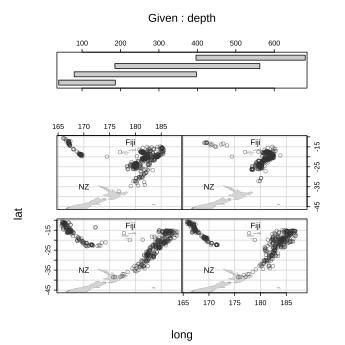
\includegraphics{gallery_files/figure-latex/coplot-1} 

}

\caption[给定震源深图的地震经纬度条件分割图]{给定震源深图的地震经纬度条件分割图:四幅散点图有相同的坐标系,震源深度按左下、右下、左上、右上的顺序逐渐增加,可以看到地震发生地点逐渐在向斐济岛靠近。}\label{fig:coplot}
\end{figure}

图 \ref{fig:coplot}
展示了斐济岛(Fiji)附近的地震数据 \texttt{quakes},数据包括地震发生地点的经纬度和震源的深度,我们想知道该地区在地震深度上分布是否均匀,因此我们令深度变量为条件变量,看在不同条件下地震发生地点(经纬度)是否有变化。从图中可以清楚看出,随着深度值的增加,地震发生地点逐渐由西向东、由南向北移动,震源较深的地震都发生在离斐济岛很近的东南侧。另外,图 \ref{fig:coplot}
还展示了 \texttt{panel} 参数的用法,我们借助 \textbf{maps} 包 \citep{maps} 在散点图上添加了新西兰和斐济岛的地图作为辅助信息,关于 R 中地图的使用请参考 \ref{sec:maps} 小节。

\section{一元函数曲线图}\label{sec:curve}





\begin{Shaded}
\begin{Highlighting}[]
\FunctionTok{par}\NormalTok{(}\AttributeTok{mar =} \FunctionTok{c}\NormalTok{(}\FloatTok{4.5}\NormalTok{, }\DecValTok{4}\NormalTok{, }\FloatTok{0.2}\NormalTok{, }\FloatTok{0.2}\NormalTok{), }\AttributeTok{mfrow =} \FunctionTok{c}\NormalTok{(}\DecValTok{2}\NormalTok{, }\DecValTok{1}\NormalTok{))}
\NormalTok{chippy }\OtherTok{\textless{}{-}} \ControlFlowTok{function}\NormalTok{(x) }\FunctionTok{sin}\NormalTok{(}\FunctionTok{cos}\NormalTok{(x) }\SpecialCharTok{*} \FunctionTok{exp}\NormalTok{(}\SpecialCharTok{{-}}\NormalTok{x }\SpecialCharTok{/} \DecValTok{2}\NormalTok{))}
\FunctionTok{curve}\NormalTok{(chippy, }\SpecialCharTok{{-}}\DecValTok{8}\NormalTok{, }\DecValTok{7}\NormalTok{, }\AttributeTok{n =} \DecValTok{2008}\NormalTok{, }\AttributeTok{xlab =} \StringTok{"$x$"}\NormalTok{, }\AttributeTok{ylab =} \StringTok{"$}\SpecialCharTok{\textbackslash{}\textbackslash{}}\StringTok{mathrm\{chippy\}(x)$"}\NormalTok{)}
\FunctionTok{curve}\NormalTok{(}\FunctionTok{sin}\NormalTok{(x) }\SpecialCharTok{/}\NormalTok{ x, }\AttributeTok{from =} \SpecialCharTok{{-}}\DecValTok{20}\NormalTok{, }\AttributeTok{to =} \DecValTok{20}\NormalTok{, }\AttributeTok{n =} \DecValTok{200}\NormalTok{, }
      \AttributeTok{xlab =} \StringTok{"$t$"}\NormalTok{, }\AttributeTok{ylab =} \StringTok{"$}\SpecialCharTok{\textbackslash{}\textbackslash{}}\StringTok{varphi\_\{X\}(t)$"}\NormalTok{)}
\end{Highlighting}
\end{Shaded}

\begin{figure}

{\centering 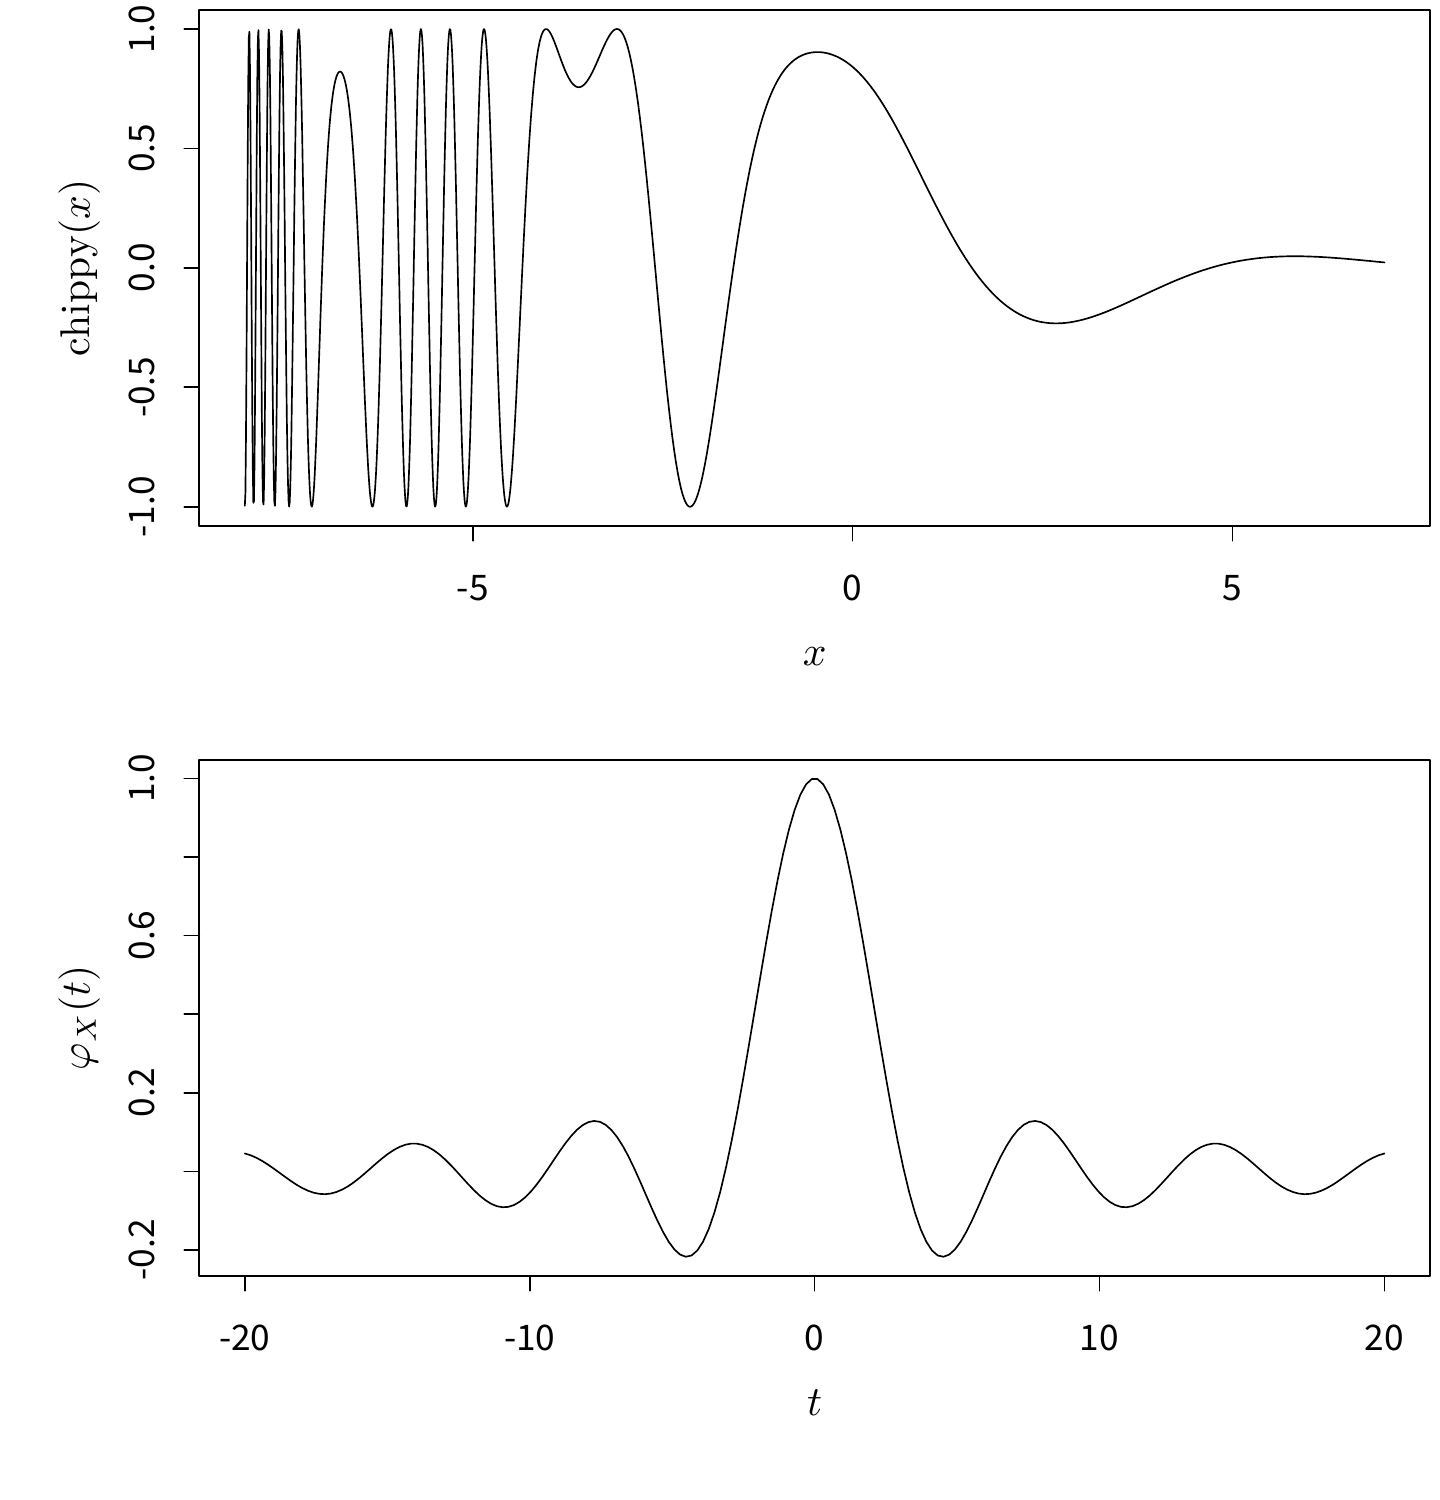
\includegraphics{gallery_files/figure-latex/curve-1} 

}

\caption[函数 \(f(x)=\mathrm{sin}(\mathrm{cos}(x)*\mathrm{exp}(-x/2))\) 的曲线图]{函数 \(f(x)=\mathrm{sin}(\mathrm{cos}(x)*\mathrm{exp}(-x/2))\) 的曲线图(上)和均匀分布 \(U(-1,1)\) 的特征函数图(下)。}\label{fig:curve}
\end{figure}

函数曲线图没有什么特殊之处,仅仅是一条曲线而已,R 专门提供了一个函数,目的是为了节省我们去使用低层作图函数(如 \texttt{lines()})的精力和时间。利用这个函数,我们可以方便地对任何一元函数作出它在某段定义域上的曲线。

R 中函数曲线图的函数为 \texttt{curve()},其用法如下:

\begin{Shaded}
\begin{Highlighting}[]
\FunctionTok{usage}\NormalTok{(curve)}
\end{Highlighting}
\end{Shaded}

\begin{verbatim}
## curve(expr, from = NULL, to = NULL, n = 101, add = FALSE, type = "l",
##   xname = "x", xlab = xname, ylab = NULL, log = NULL, xlim = NULL, ...)
\end{verbatim}

参数 \texttt{expr} 为一个一元函数或者该函数的名称; \texttt{from} 和 \texttt{to} 分别定义了曲线的起点和终点; \texttt{n} 决定将定义域分成多少个小区间,以便计算函数值并连接曲线, \texttt{n} 值越大曲线越光滑; \texttt{add} 参数决定是否将曲线添加到现有图形上; \texttt{type} 参数决定了作图类型(参见 \ref{sec:plot} 小节和图 \ref{fig:plot-type})。注意:若对一个函数直接应用 \texttt{plot()} 函数,那么泛型函数 \texttt{plot()} 会自动调用 \texttt{curve()} 完成作图。

图 \ref{fig:curve} 给出了函数 \(f(x)=\sin(\cos(x)*\exp(-x/2))\) 的曲线以及均匀分布 \(U(-1,1)\) 的特征函数曲线作为示例,其中特征函数为概率论中定义的 \(\varphi_{X}(t) = \mathrm{E}[\exp(itX)]\)。由于 \texttt{curve()} 与数据分析关系不甚密切,我们在此只是粗略介绍一下。

\section{Cleveland 点图}\label{sec:dotchart}

在前面条形图(\ref{sec:barplot} 小节)和后面饼图(\ref{sec:pie} 小节)的章节中我们提到了点图 \citep{Cleveland85},事实上点图和条形图的功能非常类似:条形图通过条的长度表示数值大小,点图通过点的位置表示数值大小,二者几乎可以在任何情况下互换。





\begin{Shaded}
\begin{Highlighting}[]
\FunctionTok{par}\NormalTok{(}\AttributeTok{mar =} \FunctionTok{c}\NormalTok{(}\DecValTok{4}\NormalTok{, }\DecValTok{4}\NormalTok{, }\FloatTok{0.2}\NormalTok{, }\FloatTok{0.2}\NormalTok{))}
\FunctionTok{dotchart}\NormalTok{(}\FunctionTok{t}\NormalTok{(VADeaths)[, }\DecValTok{5}\SpecialCharTok{:}\DecValTok{1}\NormalTok{], }\AttributeTok{col =} \FunctionTok{brewer.pal}\NormalTok{(}\DecValTok{4}\NormalTok{, }\StringTok{"Set1"}\NormalTok{), }\AttributeTok{pch =} \DecValTok{19}\NormalTok{, }\AttributeTok{cex =}\NormalTok{ .}\DecValTok{65}\NormalTok{)}
\end{Highlighting}
\end{Shaded}

\begin{figure}

{\centering 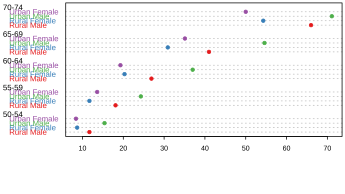
\includegraphics{gallery_files/figure-latex/dotchart-1} 

}

\caption[弗吉尼亚死亡率数据的 Cleveland 点图]{弗吉尼亚死亡率数据的 Cleveland 点图}\label{fig:dotchart}
\end{figure}

R 中点图的函数为 \texttt{dotchart()},用法如下:

\begin{Shaded}
\begin{Highlighting}[]
\FunctionTok{usage}\NormalTok{(dotchart)}
\end{Highlighting}
\end{Shaded}

\begin{verbatim}
## dotchart(x, labels = NULL, groups = NULL, gdata = NULL, offset = 1/8,
##   ann = par("ann"), xaxt = par("xaxt"), frame.plot = TRUE, log = "",
##   cex = par("cex"), pt.cex = cex, pch = 21, gpch = 21, bg = par("bg"),
##   color = par("fg"), gcolor = par("fg"), lcolor = "gray",
##   xlim = range(x[is.finite(x)]), main = NULL, xlab = NULL, ylab = NULL, ...)
\end{verbatim}

其中 \texttt{x} 与条形图的 \texttt{height} 参数相同,为一个数值向量或者矩阵; \texttt{labels} 为数据的标签;其它参数主要用来设置图形的样式如颜色、缩放倍数、点的样式等,此处略去。

图 \ref{fig:dotchart} 再次以弗吉尼亚死亡率数据为例,给出了点图的展示。对比图 \ref{fig:vadeaths-barplot} 不难发现点图与条形图的相通之处。相比之下,点图的图形元素更加简洁,制图时不会显得太拥挤,我们可以视情况在这二者选其一作为表达工具。

\section{颜色等高图/层次图}\label{sec:filled-contour}

颜色等高图,\citet{Cleveland93} 又称之为层次图(Level Plot),与等高图的原理完全类似,只是颜色等高图用不同颜色表示不同高度,并配有颜色图例,用以说明图中的颜色与高度值的对应关系。读者可以回顾 \ref{sec:contour} 小节关于等高图的介绍。





\begin{Shaded}
\begin{Highlighting}[]
\FunctionTok{demo}\NormalTok{(}\StringTok{"volcano"}\NormalTok{, }\AttributeTok{package =} \StringTok{"MSG"}\NormalTok{)}
\end{Highlighting}
\end{Shaded}

\begin{figure}

{\centering 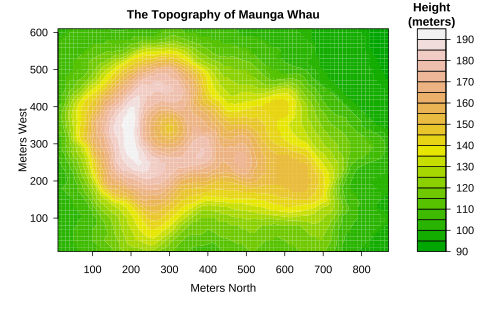
\includegraphics{gallery_files/figure-latex/filled-contour-1} 

}

\caption[新西兰 Maunga Whau 火山高度数据颜色等高图]{新西兰 Maunga Whau 火山高度数据颜色等高图}\label{fig:filled-contour}
\end{figure}

R 中的颜色等高图函数为 \texttt{filled.contour()},其用法如下:

\begin{Shaded}
\begin{Highlighting}[]
\FunctionTok{usage}\NormalTok{(filled.contour)}
\end{Highlighting}
\end{Shaded}

\begin{verbatim}
## filled.contour(x = seq(0, 1, length.out = nrow(z)),
##   y = seq(0, 1, length.out = ncol(z)), z, xlim = range(x, finite = TRUE),
##   ylim = range(y, finite = TRUE), zlim = range(z, finite = TRUE),
##   levels = pretty(zlim, nlevels), nlevels = 20,
##   color.palette = function(n) hcl.colors(n, "YlOrRd", rev = TRUE),
##   col = color.palette(length(levels) - 1), plot.title, plot.axes, key.title,
##   key.axes, key.border = NULL, asp = NA, xaxs = "i", yaxs = "i", las = 1,
##   axes = TRUE, frame.plot = axes, ...)
\end{verbatim}

这里面大多数参数与 \texttt{contour()} 函数完全相同,区别在于多了几个定义颜色的参数。 \texttt{color.palette} 给定一个调色板函数,用以生成一系列颜色供等高图填充使用,默认是青、白、粉调色板(回顾 \ref{sec:palette} 小节);如果我们不指定调色板,也可以用 col 参数指定各高度水平对应的颜色; \texttt{plot.title} 、 \texttt{plot.axes} 、 \texttt{key.title} 和 \texttt{key.axes} 四个参数分别控制着等高图的标题、等高图的坐标轴、图例的标题和图例的坐标轴,它们都能接受若干语句(statement)作为参数值。

图 \ref{fig:filled-contour}
描绘了新西兰 Maunga Whau 火山的地理数据 \texttt{volcano},这份数据包含了在 \(10\mathrm{m}\times10\mathrm{m}\) 的地理网格上测得的火山高度,是一个 \(87\times61\) 的矩阵。仔细观察图 \ref{fig:filled-contour},由于火山口的存在,颜色等高图的中部(偏左)有一小块区域的颜色并非白色,意即此处的高度比周围一圈要低。这种情况在三维图中有时未必能够迅速看出来,必须将视角调整为略向下俯视才能看到火山口。注意本图的调色板用的是''绿黄棕白''调色板,如 \ref{sec:palette} 小节所介绍的,这种调色板比较适合展示地理数据。图 \ref{fig:persp-pop}
提供了真实的火山立体图形。

颜色等高图中的图形布局(等高图和图例实质上都是独立的图形)是用 \texttt{layout()} 函数(\ref{sec:multipage} 小节)完成的,这给我们带来了扩展上的不便,主要是因为颜色等高图的坐标系统与单幅统计图形的坐标系统并不一样,例如我们无法在作完一幅等高图之后再往图中添加诸如标题、坐标轴等图形元素,这种情况下,我们不妨采用另一种类似的图形--- 颜色图,参见 \ref{sec:image} 小节。

\section{四瓣图}\label{sec:fourfoldplot}

四瓣图(Fourfold Plot)是用来查看 \(2\times2\times k\) 列联表中两个二分变量之间关联关系的一种图示工具,它主要是基于二维列联表的检验理论而建立起来的 \citep{Friendly94}。

表 \ref{tab:contingency} 是一个典型的二维列联表,通常我们想检验的是行变量与列变量是否独立;前面 \ref{sec:assocplot} 小节中曾经利用 \(\chi^{2}\) 检验构造了关联图,这里我们从优比(Odds Ratio,OR)的角度出发对列联表进行检验。

首先我们定义以下二式分别为在因素出现和不出现的情况下事件的发生率(医学上常称为风险):

\begin{equation} 
\frac{P_{1}}{P_{1}+P_{3}};\;\;\frac{P_{2}}{P_{2}+P_{4}}
\label{eq:OR1}
\end{equation}

进而我们用这二式之比得到优比:

\begin{equation} 
\mathrm{OR}\equiv\frac{P_{1}}{P_{1}+P_{3}}/\frac{P_{2}}{P_{2}+P_{4}}=\frac{P_{1}(P_{2}+P_{4})}{P_{2}(P_{1}+P_{3})}
\label{eq:OR}
\end{equation}

\begin{longtable}[]{@{}rcl@{}}
\caption{\label{tab:contingency} 二维列联表的经典形式}\tabularnewline
\toprule\noalign{}
& 事件 & \\
\midrule\noalign{}
\endfirsthead
\toprule\noalign{}
& 事件 & \\
\midrule\noalign{}
\endhead
\bottomrule\noalign{}
\endlastfoot
& 发生  不发生 & \\
因素 有 & \(P_{1}\)  \(P_{3}\) & \(P_{1}+P_{3}\) \\
无 & \(P_{2}\)  \(P_{4}\) & \(P_{2}+P_{4}\) \\
& \(P_{1}+P_{2}\) \(P_{3}+P_{4}\) & \\
\end{longtable}

由于通常情况下事件发生的几率都比较小(尤其是医学上的疾病),即 \(P_{1}\) 相对 \(P_{3}\) 来说较小,\(P_{2}\) 相对 \(P_{4}\) 来说较小,因此 \eqref{eq:OR} 式可以近似用 \eqref{eq:ORapprox} 式代替:

\begin{equation} 
\mathrm{OR}\approx\Psi\equiv\frac{P_{1}P_{4}}{P_{2}P_{3}}
\label{eq:ORapprox}
\end{equation}

我们记各单元格的样本实现值分别为 \(a,b,c,d\);如果事件和因素相互独立,那么因素是否发生对事件是否发生(或发生率)没有影响,因此在零假设下优比的样本实现值 \(ad/bc\) 应该接近于 1,换句话说,如果优比与 1 显著不同,那么很可能行列变量不独立。

四瓣图正是基于这样一个比例来完成制图的,它将优比体现在两个相邻的四分之一圆的半径之比上,如果两个扇形半径差异显著,那么说明行列变量不独立,即因素对事件有影响,这便是四瓣图最基本的用法,而背后还有关于优比置信区间的计算,并且这个置信区间也在图中用两道弧线表现了出来,四瓣图最终的读法就是观察两瓣相邻扇形的置信区间弧线是否有重叠,有则说明不能拒绝零假设,反之可以拒绝。这是基于假设检验和区间估计之间的转换关系而得以成立的。

计算置信区间需要用到 \(\Psi\) 的方差以及正态性假定;\(\Psi\) 的方差并不容易直接计算,但取对数之后就很容易了:

\begin{equation}
\mathrm{Var}(\mathrm{log}(\Psi))=\frac{1}{a}+\frac{1}{b}+\frac{1}{c}+\frac{1}{d}
\label{eq:ORlog}
\end{equation}

其置信区间为:

\begin{equation}
\mathrm{log}(\Psi)\pm q_{1-\alpha/2}\sqrt{\mathrm{Var}(\mathrm{log}(\Psi))}
\label{eq:ORconf}
\end{equation}

通过对 \eqref{eq:ORconf} 取指数即可还原到 \(\Psi\) 本身的置信区间。关于四瓣图的数学理论就介绍到这里,感兴趣的读者可以参阅 \citet{Friendly94} 或者直接阅读 \texttt{fourfoldplot()} 的源代码(大约 200 行)。

R 中四瓣图函数 \texttt{fourfoldplot()} 的用法如下:

\begin{Shaded}
\begin{Highlighting}[]
\FunctionTok{usage}\NormalTok{(fourfoldplot)}
\end{Highlighting}
\end{Shaded}

\begin{verbatim}
## fourfoldplot(x, color = c("#99CCFF", "#6699CC"), conf.level = 0.95,
##   std = c("margins", "ind.max", "all.max"), margin = c(1, 2), space = 0.2,
##   main = NULL, mfrow = NULL, mfcol = NULL)
\end{verbatim}

其中 \texttt{x} 是一个 \(2\times2\times k\) 的数组,当 \(k=1\) 时,它也可以直接取一个 \(2\times2\) 的矩阵; \texttt{color} 设定四分之一圆的填充颜色,处于同一对角线上的扇形颜色相同,颜色填充的顺序也反映出优比与 1 的大小; \texttt{onf.level} 为置信水平; \texttt{std} 为列联表的标准化方法,决定了标准化时分母所除的数。当 \(k\geq1\) 时,该函数会依次生成 \(k\) 幅四瓣图。





\begin{Shaded}
\begin{Highlighting}[]
\FunctionTok{ftable}\NormalTok{(UCBAdmissions) }\CommentTok{\# 以紧凑形式展现出来的 UCB 录取数据}
\end{Highlighting}
\end{Shaded}

\begin{verbatim}
##                 Dept   A   B   C   D   E   F
## Admit    Gender                             
## Admitted Male        512 353 120 138  53  22
##          Female       89  17 202 131  94  24
## Rejected Male        313 207 205 279 138 351
##          Female       19   8 391 244 299 317
\end{verbatim}

\begin{Shaded}
\begin{Highlighting}[]
\FunctionTok{fourfoldplot}\NormalTok{(UCBAdmissions, }\AttributeTok{mfcol =} \FunctionTok{c}\NormalTok{(}\DecValTok{2}\NormalTok{, }\DecValTok{3}\NormalTok{)) }\CommentTok{\# 2 行 3 列排版}
\end{Highlighting}
\end{Shaded}

\begin{figure}

{\centering \includegraphics{gallery_files/figure-latex/fourfoldplot-1} 

}

\caption[加州伯克利分校录取数据四瓣图]{加州伯克利分校录取数据四瓣图}\label{fig:fourfoldplot}
\end{figure}

图 \ref{fig:fourfoldplot} 是加州伯克利分校(UCB)录取数据的四瓣图,数据见于图中的代码输出。这批数据为一个 \(2\times2\times6\) 的数组,我们可以分系别来看学生的录取是否与性别有关。从图中反映的情况来看,只有 A 系的四瓣图显示出了置信区间弧线不相交的情况,说明 A 系学生的录取与性别不独立,而其它系都不能拒绝零假设''录取与性别无关''。

现在我们不妨通过一些简单的 R 语言计算来证实两件事情。首先是扇形颜色的填充与优比的关系,计算优比的代码如下:

\begin{Shaded}
\begin{Highlighting}[]
\NormalTok{(x }\OtherTok{\textless{}{-}} \FunctionTok{apply}\NormalTok{(UCBAdmissions, }\DecValTok{3}\NormalTok{, }\ControlFlowTok{function}\NormalTok{(x) (x[}\DecValTok{1}\NormalTok{, }\DecValTok{1}\NormalTok{] }\SpecialCharTok{*}\NormalTok{ x[}\DecValTok{2}\NormalTok{, }\DecValTok{2}\NormalTok{]) }\SpecialCharTok{/}\NormalTok{ (x[}\DecValTok{1}\NormalTok{, }\DecValTok{2}\NormalTok{] }\SpecialCharTok{*}\NormalTok{ x[}\DecValTok{2}\NormalTok{, }\DecValTok{1}\NormalTok{])))}
\end{Highlighting}
\end{Shaded}

\begin{verbatim}
##         A         B         C         D         E         F 
## 0.3492120 0.8025007 1.1330596 0.9212838 1.2216312 0.8278727
\end{verbatim}

C 和 E 系的优比大于 1,观察图 \ref{fig:fourfoldplot} 可知, \texttt{color} 参数的第一个颜色值填充第一、三象限的扇形,而优比小于 1 时,第一个颜色值填充第二、四象限。

其次我们完全可以将优比的置信区间分别算出来,看它们是否包含数值 1:

\begin{Shaded}
\begin{Highlighting}[]
\NormalTok{y }\OtherTok{\textless{}{-}} \FunctionTok{qnorm}\NormalTok{(}\FloatTok{0.975}\NormalTok{) }\SpecialCharTok{*} \FunctionTok{sqrt}\NormalTok{(}\FunctionTok{apply}\NormalTok{(UCBAdmissions, }\DecValTok{3}\NormalTok{, }\ControlFlowTok{function}\NormalTok{(x) \{}
  \FunctionTok{sum}\NormalTok{(}\DecValTok{1} \SpecialCharTok{/}\NormalTok{ x)}
\NormalTok{\}))}
\NormalTok{conf }\OtherTok{\textless{}{-}} \FunctionTok{exp}\NormalTok{(}\FunctionTok{cbind}\NormalTok{(}\FunctionTok{log}\NormalTok{(x) }\SpecialCharTok{{-}}\NormalTok{ y, }\FunctionTok{log}\NormalTok{(x) }\SpecialCharTok{+}\NormalTok{ y))}
\FunctionTok{colnames}\NormalTok{(conf) }\OtherTok{\textless{}{-}} \FunctionTok{c}\NormalTok{(}\StringTok{"2.5\%"}\NormalTok{, }\StringTok{"97.5\%"}\NormalTok{)}
\NormalTok{conf}
\end{Highlighting}
\end{Shaded}

\begin{verbatim}
##        2.5%     97.5%
## A 0.2086756 0.5843954
## B 0.3403815 1.8920166
## C 0.8545328 1.5023696
## D 0.6863345 1.2366620
## E 0.8250748 1.8087848
## F 0.4552059 1.5056335
\end{verbatim}

显然,这些置信区间中只有 A 系的不包含 1 在内,因此对于该系来说可以拒绝零假设。这与图形得到的结论是完全相符的。这里我们提醒读者注意上面的 R 代码与数学公式的对应关系,很多时候根据数学公式写 R 代码是非常简单的工作。最后我们可以看看卡方检验的 P 值,这些 P 值对应的结论和上面的图形和优比的结论都相同:

\begin{Shaded}
\begin{Highlighting}[]
\CommentTok{\# 对每个系的录取数据进行卡方检验分别得到 P 值}
\FunctionTok{round}\NormalTok{(}\FunctionTok{apply}\NormalTok{(UCBAdmissions, }\DecValTok{3}\NormalTok{, }\ControlFlowTok{function}\NormalTok{(x) }\FunctionTok{chisq.test}\NormalTok{(x)}\SpecialCharTok{$}\NormalTok{p.value), }\DecValTok{3}\NormalTok{)}
\end{Highlighting}
\end{Shaded}

\begin{verbatim}
##     A     B     C     D     E     F 
## 0.000 0.771 0.426 0.638 0.369 0.640
\end{verbatim}

\section{颜色图}\label{sec:image}





\begin{Shaded}
\begin{Highlighting}[]
\FunctionTok{par}\NormalTok{(}\AttributeTok{mar =} \FunctionTok{rep}\NormalTok{(}\DecValTok{0}\NormalTok{, }\DecValTok{4}\NormalTok{))}
\NormalTok{x }\OtherTok{\textless{}{-}} \FunctionTok{matrix}\NormalTok{(}\FunctionTok{sample}\NormalTok{(}\DecValTok{24}\NormalTok{), }\DecValTok{8}\NormalTok{)}
\FunctionTok{image}\NormalTok{(}\DecValTok{1}\SpecialCharTok{:}\DecValTok{8}\NormalTok{, }\DecValTok{1}\SpecialCharTok{:}\DecValTok{3}\NormalTok{, x, }\AttributeTok{col =} \FunctionTok{heat.colors}\NormalTok{(}\DecValTok{24}\NormalTok{), }\AttributeTok{axes =} \ConstantTok{FALSE}\NormalTok{, }\AttributeTok{ann =} \ConstantTok{FALSE}\NormalTok{)}
\FunctionTok{text}\NormalTok{(}\FunctionTok{rep}\NormalTok{(}\DecValTok{1}\SpecialCharTok{:}\DecValTok{8}\NormalTok{, }\DecValTok{3}\NormalTok{), }\FunctionTok{rep}\NormalTok{(}\DecValTok{1}\SpecialCharTok{:}\DecValTok{3}\NormalTok{, }\AttributeTok{each =} \DecValTok{8}\NormalTok{), }\FunctionTok{as.vector}\NormalTok{(x))}
\end{Highlighting}
\end{Shaded}

\begin{figure}

{\centering \includegraphics{gallery_files/figure-latex/image24-1} 

}

\caption[颜色图中色块与数值的对应关系]{颜色图中色块与数值的对应关系:矩阵中数值越大,色块越趋近于白色,反之趋近红色。}\label{fig:image24}
\end{figure}

颜色图(Color Image)与颜色等高图看起来非常类似,但是等高图需要从网格矩阵中计算等高的数据点,有时还需要一些平滑处理,而颜色图并不涉及任何背后的计算,只是简单将一个网格矩阵映射到指定的颜色序列上、以颜色方块表示数据的大小。在数据规律性较强且数据量较大的时候,这两种图形的区别可以说微乎其微,而当数据没什么规律或者数据量比较小的时候,颜色图的色块就可以很清楚地显露出来了,图 \ref{fig:image24}
为一个简单的示意图。

R 中颜色图的函数为 \texttt{image()},其用法如下:

\begin{Shaded}
\begin{Highlighting}[]
\FunctionTok{usage}\NormalTok{(image.default)}
\end{Highlighting}
\end{Shaded}

\begin{verbatim}
## ## Default S3 method:
## image(x = seq(0, 1, length.out = nrow(z)), y = seq(0, 1, length.out = ncol(z)),
##   z, zlim = range(z[is.finite(z)]), xlim = range(x), ylim = range(y),
##   col = hcl.colors(12, "YlOrRd", rev = TRUE), add = FALSE, xaxs = "i",
##   yaxs = "i", xlab, ylab, breaks, oldstyle = FALSE, useRaster, ...)
\end{verbatim}

参数 \texttt{x} 、 \texttt{y} 、 \texttt{z} 与等高线的参数类似,不过由于该函数为泛型函数,因此也可以接受不同类型的参数,这三个参数除了可以接受两个数值向量和一个矩阵之外, \texttt{x} 还可以接受一个列表,列表中包含三个子对象:\texttt{x\$x}、\texttt{x\$y} 和 \texttt{x\$z},这三个子对象分别为两个数值向量和一个矩阵,这种情况下就不需要另外单独提供 \texttt{y} 和 \texttt{z} 参数了; \texttt{col} 设置一个颜色序列以便映射到不同大小的数值; \texttt{add} 为逻辑值,决定是否将颜色图添加到现有图形上; \texttt{breaks} 给定 \texttt{z} 分段的区间端点。





\begin{Shaded}
\begin{Highlighting}[]
\FunctionTok{par}\NormalTok{(}\AttributeTok{mar =} \FunctionTok{rep}\NormalTok{(}\DecValTok{0}\NormalTok{, }\DecValTok{4}\NormalTok{), }\AttributeTok{ann =} \ConstantTok{FALSE}\NormalTok{)}
\NormalTok{x }\OtherTok{\textless{}{-}} \DecValTok{10} \SpecialCharTok{*}\NormalTok{ (}\DecValTok{1}\SpecialCharTok{:}\FunctionTok{nrow}\NormalTok{(volcano))}
\NormalTok{y }\OtherTok{\textless{}{-}} \DecValTok{10} \SpecialCharTok{*}\NormalTok{ (}\DecValTok{1}\SpecialCharTok{:}\FunctionTok{ncol}\NormalTok{(volcano))}
\FunctionTok{image}\NormalTok{(x, y, volcano, }\AttributeTok{col =} \FunctionTok{terrain.colors}\NormalTok{(}\DecValTok{100}\NormalTok{), }\AttributeTok{axes =} \ConstantTok{FALSE}\NormalTok{)}
\FunctionTok{contour}\NormalTok{(x, y, volcano,}
  \AttributeTok{levels =} \FunctionTok{seq}\NormalTok{(}\DecValTok{90}\NormalTok{, }\DecValTok{200}\NormalTok{, }\AttributeTok{by =} \DecValTok{5}\NormalTok{),}
  \AttributeTok{add =} \ConstantTok{TRUE}\NormalTok{, }\AttributeTok{col =} \StringTok{"peru"}
\NormalTok{)}
\FunctionTok{box}\NormalTok{()}
\end{Highlighting}
\end{Shaded}

\begin{figure}

{\centering \includegraphics{gallery_files/figure-latex/image-1} 

}

\caption[新西兰 Maunga Whau 火山高度数据颜色图]{新西兰 Maunga Whau 火山高度颜色图:图 \ref{fig:persp} 提供了真实的火山立体图形;读者可以到作者个人主页下载原图并放大 8 倍以上查看颜色图和颜色等高图的区别:颜色图是用颜色填充方块,而颜色等高图则是用颜色填充等高线之间的区域。}\label{fig:image}
\end{figure}

这里我们仍然以新西兰 Maunga Whau 火山高度数据 \texttt{volcano} 为例。图 \ref{fig:image}
是火山数据的颜色图,从外观上来看,它与前面的颜色等高图几乎无异(图 \ref{fig:filled-contour}),但图 \ref{fig:image} 中多了一些等高线,这也说明了颜色图较之颜色等高图的灵活性和可扩展性。在 \ref{sec:filled-contour} 小节的最后我们曾提到颜色等高图作完之后就不容易再往图中添加图形元素,而这里颜色图只是单幅图形,作完之后仍然可以方便地添加图形元素。

统计数据中有不少是矩阵形式,例如相关系数阵、协方差阵等,我们可以将颜色图应用到这些矩阵形式数据的展示上,尤其是当矩阵行数列数较大时,我们可以借助人眼对颜色的视觉感知从颜色图中迅速找出一定的统计特征来(如很大或者很小的数值),而相比之下,对数据的直接观察并不容易找到规律或特征,因为这种形式下我们必须在脑中对数据两两比较,其速度必然会很慢。

\textbf{lattice} 包 \citep{Sarkar08} 中提供了一个类似的函数 \texttt{levelplot()},展示方法更为灵活,感兴趣的读者请参考函数的帮助文件。

\section{矩阵图、矩阵点、矩阵线}\label{sec:matplot}





\begin{Shaded}
\begin{Highlighting}[]
\NormalTok{sines }\OtherTok{\textless{}{-}} \FunctionTok{outer}\NormalTok{(}\DecValTok{1}\SpecialCharTok{:}\DecValTok{20}\NormalTok{, }\DecValTok{1}\SpecialCharTok{:}\DecValTok{4}\NormalTok{, }\ControlFlowTok{function}\NormalTok{(x, y) }\FunctionTok{sin}\NormalTok{(x }\SpecialCharTok{/} \DecValTok{20} \SpecialCharTok{*}\NormalTok{ pi }\SpecialCharTok{*}\NormalTok{ y))}
\FunctionTok{par}\NormalTok{(}\AttributeTok{mar =} \FunctionTok{c}\NormalTok{(}\DecValTok{2}\NormalTok{, }\DecValTok{4}\NormalTok{, .}\DecValTok{1}\NormalTok{, .}\DecValTok{1}\NormalTok{))}
\FunctionTok{matplot}\NormalTok{(sines, }\AttributeTok{type =} \StringTok{"b"}\NormalTok{, }\AttributeTok{pch =} \DecValTok{21}\SpecialCharTok{:}\DecValTok{24}\NormalTok{, }\AttributeTok{col =} \DecValTok{2}\SpecialCharTok{:}\DecValTok{5}\NormalTok{, }\AttributeTok{bg =} \DecValTok{2}\SpecialCharTok{:}\DecValTok{5}\NormalTok{)}
\end{Highlighting}
\end{Shaded}

\begin{figure}

{\centering \includegraphics{gallery_files/figure-latex/matplot-1} 

}

\caption[用矩阵图画出的一系列正弦曲线]{用矩阵图画出的一系列正弦曲线:每条曲线都有不同的点线样式和颜色。}\label{fig:matplot}
\end{figure}

\begin{Shaded}
\begin{Highlighting}[]
\CommentTok{\# 数据矩阵的前 6 行}
\FunctionTok{round}\NormalTok{(}\FunctionTok{head}\NormalTok{(sines), }\DecValTok{5}\NormalTok{)}
\end{Highlighting}
\end{Shaded}

\begin{verbatim}
##         [,1]    [,2]    [,3]     [,4]
## [1,] 0.15643 0.30902 0.45399  0.58779
## [2,] 0.30902 0.58779 0.80902  0.95106
## [3,] 0.45399 0.80902 0.98769  0.95106
## [4,] 0.58779 0.95106 0.95106  0.58779
## [5,] 0.70711 1.00000 0.70711  0.00000
## [6,] 0.80902 0.95106 0.30902 -0.58779
\end{verbatim}

矩阵图的名称来自于其参数类型,它可以针对一个矩阵将所有列以曲线的形式表达出来,同一元函数曲线图(\ref{sec:curve} 小节)一样,它也没有什么特别之处,仅仅是提供了一个便利的封装,我们可以不必调用 \texttt{lines()} 等函数依次对矩阵的所有列画曲线。

R 中矩阵图的函数为 \texttt{matplot()},矩阵点的函数为 \texttt{matpoints()},矩阵线的函数为 \texttt{matlines()},它们的用法如下:

\begin{Shaded}
\begin{Highlighting}[]
\FunctionTok{usage}\NormalTok{(matplot)}
\end{Highlighting}
\end{Shaded}

\begin{verbatim}
## matplot(x, y, type = "p", lty = 1:5, lwd = 1, lend = par("lend"), pch = NULL,
##   col = 1:6, cex = NULL, bg = NA, xlab = NULL, ylab = NULL, xlim = NULL,
##   ylim = NULL, log = "", ..., add = FALSE, verbose = getOption("verbose"))
\end{verbatim}

\begin{Shaded}
\begin{Highlighting}[]
\FunctionTok{usage}\NormalTok{(matpoints)}
\end{Highlighting}
\end{Shaded}

\begin{verbatim}
## matpoints(x, y, type = "p", lty = 1:5, lwd = 1, pch = NULL, col = 1:6, ...)
\end{verbatim}

\begin{Shaded}
\begin{Highlighting}[]
\FunctionTok{usage}\NormalTok{(matlines)}
\end{Highlighting}
\end{Shaded}

\begin{verbatim}
## matlines(x, y, type = "l", lty = 1:5, lwd = 1, pch = NULL, col = 1:6, ...)
\end{verbatim}

函数 \texttt{matplot()} 为高层作图函数(创建新图形),而后两个函数均为低层作图函数(向现有图形上添加元素)。参数 \texttt{x} 和 \texttt{y} 为输入的矩阵,做图的方式是用 \texttt{x} 的列为横轴方向的变量, \texttt{y} 的列为纵轴方向的变量,然后用这些列依次作散点图( \texttt{x} 的第一列对 y 的第一列, \texttt{x} 的第二列对 \texttt{y} 的第二列,依次类推);如果这两个参数有一个缺失,那么 x 将被 \texttt{1:nrow(y)} 代替, \texttt{y} 被非缺失的参数矩阵代替;注意两个矩阵要么有一个列数为 1,要么列数相等,否则会报错;后面设置颜色、线型等样式的参数 \texttt{type} 、 \texttt{lty} 、 \texttt{lwd} 、 \texttt{pch} 、 \texttt{col} 、 \texttt{cex} 、 \texttt{bg} 等在附录 \ref{cha:tricks} 和第 \ref{cha:elements} 章已经讲述过多次,此处不再赘述。

图 \ref{fig:matplot}
展示了一个正弦值矩阵的矩阵图。从图上方的代码中我们可以看到矩阵的前 6 行数值,该例中只给出了参数 \texttt{x} 而没有 \texttt{y},所以 \texttt{matplot()} 用矩阵 \texttt{sines} 的每一列依次和 \texttt{1:20} 画曲线。

\section{马赛克图}\label{sec:mosaicplot}

马赛克图(Mosaic Plots)是展示多维列联表数据的工具。前面我们已经提到过两种展示列联表数据的工具(\ref{sec:assocplot} 和 \ref{sec:fourfoldplot} 小节),但它们都只能展示低维列联表,而马赛克图对于列联表的维数没有限制。

马赛克图的表现形式为与频数成比例的矩形块,整幅图形看起来就像是若干块马赛克放置在平面上。马赛克图背后的统计理论是对数线性模型(log-linear model),我们先回顾一个最简单的二维列联表的独立模型。

二维列联表的独立性从概率角度来说就是单元格的频率等于边际频率的乘积:

\begin{equation}
\pi_{ij}=\pi_{i\cdot}\pi_{\cdot j}
\label{eq:independence}
\end{equation}

取对数即得:

\begin{equation}
\mathrm{log}(\pi_{ij})=\mathrm{log}(\pi_{i\cdot})+\mathrm{log}(\pi_{\cdot j})
\label{eq:logindependence}
\end{equation}

根据 \(\mu_{ij}=n\pi_{ij}\) 进一步写成频数的形式:

\begin{equation}
\mathrm{log}(\mu_{ij})=\lambda+\lambda_{i}^{r}+\lambda_{j}^{c}
\label{eq:freqindependence}
\end{equation}

\(\lambda_{i}^{r}\) 和 \(\lambda_{j}^{c}\) 分别表示行效应和列效应,\(\lambda\) 为常数。 \eqref{eq:freqindependence} 式就是最普通的对数线性模型,通过计算拟合,我们可以得到行列效应的估计值。对数线性模型在马赛克图中的主要表现是单元格的残差,而单元格的残差可以有三种:似然比残差(离差,deviance)\(G^{2}\)、Pearson \(\chi^{2}\) 残差和 Freeman-Tukey 残差,前两种定义如下式:

\begin{equation}
G^{2}=2\sum n_{ij}\mathrm{log}(\frac{n_{ij}}{\hat{\mu}_{ij}});\;\;\chi^{2}=\sum\frac{\left(n_{ij}-\hat{\mu}_{ij}\right)^{2}}{\hat{\mu}_{ij}}
\label{eq:loglinearres}
\end{equation}

残差反映的是某个单元格拟合的好坏,马赛克图用 5 级颜色表达了残差的大小,后面我们结合具体例子说明。

R 中马赛克图的函数为 \texttt{mosaicplot()} ,其用法如下:

\begin{Shaded}
\begin{Highlighting}[]
\FunctionTok{usage}\NormalTok{(graphics}\SpecialCharTok{:::}\NormalTok{mosaicplot.default)}
\end{Highlighting}
\end{Shaded}

\begin{verbatim}
## ## Default S3 method:
## mosaicplot(x, main = deparse1(substitute(x)), sub = NULL, xlab = NULL,
##   ylab = NULL, sort = NULL, off = NULL, dir = NULL, color = NULL,
##   shade = FALSE, margin = NULL, cex.axis = 0.66, las = par("las"),
##   border = NULL, type = c("pearson", "deviance", "FT"), ...)
\end{verbatim}

\begin{Shaded}
\begin{Highlighting}[]
\FunctionTok{usage}\NormalTok{(graphics}\SpecialCharTok{:::}\NormalTok{mosaicplot.formula)}
\end{Highlighting}
\end{Shaded}

\begin{verbatim}
## ## S3 method for class 'formula'
## mosaicplot(formula, data = NULL, ..., main = deparse1(substitute(data)),
##   subset, na.action = stats::na.omit)
\end{verbatim}

马赛克图函数是泛型函数,可以直接接受列联表数据或者公式作为参数,这里我们只介绍前一种情况。 \texttt{x} 为一个列联表数据(可以用函数 \texttt{table()} 生成); \texttt{main} 、 \texttt{sub} 、 \texttt{xlab} 和 \texttt{ylab} 分别设定主标题、副标题和坐标轴标题; \texttt{sort} 指定展示变量的顺序; \texttt{dir} 指定马赛克图的拆分方向(横向拆分或纵向拆分); \texttt{type} 给定残差的类型,即如前所述的三种残差。

下面我们结合泰坦尼克号数据 \texttt{Titanic} 来说明马赛克图的用法。泰坦尼克号乘客生存情况的原始数据如下:

\begin{Shaded}
\begin{Highlighting}[]
\FunctionTok{ftable}\NormalTok{(Titanic)}
\end{Highlighting}
\end{Shaded}

\begin{verbatim}
##                    Survived  No Yes
## Class Sex    Age                   
## 1st   Male   Child            0   5
##              Adult          118  57
##       Female Child            0   1
##              Adult            4 140
## 2nd   Male   Child            0  11
##              Adult          154  14
##       Female Child            0  13
##              Adult           13  80
## 3rd   Male   Child           35  13
##              Adult          387  75
##       Female Child           17  14
##              Adult           89  76
## Crew  Male   Child            0   0
##              Adult          670 192
##       Female Child            0   0
##              Adult            3  20
\end{verbatim}

该数据给出了分舱位(一二三等舱和船员舱)、分性别(男女)、分年龄(大人小孩)的生存情况。泰坦尼克号的沉没是一件著名的历史事件,至今仍然有很多人在研究它。我们所关心的问题主要是通过一些比例看出当时救援的侧重性,如:是否头等舱的乘客生还比例最高?``女士和孩子优先'' 的原则在各船舱有没有被很好遵守?\ldots\ldots{}





\begin{Shaded}
\begin{Highlighting}[]
\FunctionTok{par}\NormalTok{(}\AttributeTok{mar =} \FunctionTok{c}\NormalTok{(}\DecValTok{2}\NormalTok{, }\FloatTok{3.5}\NormalTok{, .}\DecValTok{1}\NormalTok{, .}\DecValTok{1}\NormalTok{))}
\FunctionTok{mosaicplot}\NormalTok{(Titanic, }\AttributeTok{shade =} \ConstantTok{TRUE}\NormalTok{, }\AttributeTok{main =} \StringTok{""}\NormalTok{)}
\end{Highlighting}
\end{Shaded}

\begin{figure}

{\centering \includegraphics{gallery_files/figure-latex/mosaicplot-1} 

}

\caption[泰坦尼克号乘客生存数据马赛克图]{泰坦尼克号乘客生存数据马赛克图:按性别、年龄和船舱等级划分}\label{fig:mosaicplot}
\end{figure}

图 \ref{fig:mosaicplot} 以马赛克图的形式将这个 \(4\times2\times2\times2\) 的列联表数据展示在了同一张图中,通过矩形块(马赛克)的大小,我们可以清楚看出各舱位、不同性别、年龄的人群的生还状况。例如,对头等舱来说,无论是大人小孩或男女,下方的矩形都比上方的矩形要高(尤其是女性和小孩),这说明头等舱的生还率相对来说都比较高,很可能当时的救援是偏向头等舱的;从年龄来说,头等舱和二等舱中小孩的生存率要远高于大人,但三等舱中小孩的生存率和大人相比差异并不是太显著;但从性别角度来看,各舱位基本上还是将生存机会优先让给女性了,男性的生还率在各舱位来说都相对较低。类似地,我们还可以从图中挖掘出更多的现象,这里不再深入。另外,图中用不同颜色表示出了个单元格的残差大小,其中虚线框表示残差为负数,我们可以清楚看出哪些单元格的拟合欠佳。感兴趣的读者还可以使用 \textbf{stats} 包中的 \texttt{loglin()} 函数拟合对数线性模型、从统计模型的角度继续分析。

\section{散点图矩阵}\label{sec:scatterplot-matrix}

散点图矩阵(Scatterplot Matrices)是散点图的高维扩展,它的基本构成是普通散点图,只是将多个变量的两两散点图以矩阵的形式排列起来,就构成了所谓的散点图矩阵,它通常包含 \(p\times p\) 个窗格(\(p\) 为变量个数)。散点图矩阵从一定程度上克服了在平面上展示高维数据的困难,对于我们查看变量之间的两两关系非常有用。

R 中散点图矩阵的函数为 \texttt{pairs()} ,其用法如下:

\begin{Shaded}
\begin{Highlighting}[]
\FunctionTok{usage}\NormalTok{(pairs.default)}
\end{Highlighting}
\end{Shaded}

\begin{verbatim}
## ## Default S3 method:
## pairs(x, labels, panel = points, ..., horInd = 1:nc, verInd = 1:nc,
##   lower.panel = panel, upper.panel = panel, diag.panel = NULL,
##   text.panel = textPanel, label.pos = 0.5 + has.diag/3, line.main = 3,
##   cex.labels = NULL, font.labels = 1, row1attop = TRUE, gap = 1, log = "",
##   horOdd = !row1attop, verOdd = !row1attop)
\end{verbatim}

\begin{Shaded}
\begin{Highlighting}[]
\FunctionTok{usage}\NormalTok{(graphics}\SpecialCharTok{:::}\NormalTok{pairs.formula)}
\end{Highlighting}
\end{Shaded}

\begin{verbatim}
## ## S3 method for class 'formula'
## pairs(formula, data = NULL, ..., subset, na.action = stats::na.pass)
\end{verbatim}

散点图矩阵函数是泛型函数,可以直接接受数据矩阵或者公式作为参数。 \texttt{x} 是一个矩阵或数据框,包含了要作散点图的那些变量; \texttt{labels} 是变量名称(标签); \texttt{panel} 参数给定一个画散点图的函数,这个函数将应用在每一格图形中;有时候我们并不需要统一的散点图函数,这时可以利用 \texttt{lower.panel} 和 \texttt{upper.panel} 来分别指定上三角窗格和下三角窗格中的作图函数,也就意味着上三角和下三角窗格中的图形(不一定非得是散点图)可以不一样; \texttt{diag.panel} 和 \texttt{text.panel} 分别指定对角线窗格上的作图函数和添加文本标签的函数; \texttt{label.pos} 指定文本标签的位置; \texttt{cex.labels} 指定标签的缩放倍数; \texttt{font.labels} 指定标签的字体样式; \texttt{row1attop} 为逻辑值,指定散点图的第 1 行出现在顶部还是底部(按常规讲,前者是矩阵的形式,后者是图的形式,因为矩阵通常是从上至下、从左至右,而图的坐标是从下至上、从左至右); \texttt{gap} 设定窗格之间的间距大小。

图 \ref{fig:pairs}
是对鸢尾花数据 \texttt{iris} 所作的散点图矩阵,注意其中的上三角和下三角作图函数是如何定义的。对角线窗格显示的是自定义的直方图,定义如下:

\begin{Shaded}
\begin{Highlighting}[]
\CommentTok{\# 观察如何使用 hist() 做计算并用 rect() 画图}
\NormalTok{panel.hist }\OtherTok{\textless{}{-}} \ControlFlowTok{function}\NormalTok{(x, ...) \{}
\NormalTok{  h }\OtherTok{\textless{}{-}} \FunctionTok{hist}\NormalTok{(x, }\AttributeTok{plot =} \ConstantTok{FALSE}\NormalTok{)}
\NormalTok{  nB }\OtherTok{\textless{}{-}} \FunctionTok{length}\NormalTok{(breaks }\OtherTok{\textless{}{-}}\NormalTok{ h}\SpecialCharTok{$}\NormalTok{breaks)}
\NormalTok{  y }\OtherTok{\textless{}{-}}\NormalTok{ h}\SpecialCharTok{$}\NormalTok{counts }\SpecialCharTok{/} \FunctionTok{max}\NormalTok{(h}\SpecialCharTok{$}\NormalTok{counts)}
  \FunctionTok{rect}\NormalTok{(breaks[}\SpecialCharTok{{-}}\NormalTok{nB], }\DecValTok{0}\NormalTok{, breaks[}\SpecialCharTok{{-}}\DecValTok{1}\NormalTok{], y, }\AttributeTok{col =} \StringTok{"beige"}\NormalTok{)}
\NormalTok{\}}
\end{Highlighting}
\end{Shaded}





\begin{Shaded}
\begin{Highlighting}[]
\NormalTok{idx }\OtherTok{\textless{}{-}} \FunctionTok{as.integer}\NormalTok{(iris[[}\StringTok{"Species"}\NormalTok{]])}
\FunctionTok{pairs}\NormalTok{(iris[}\DecValTok{1}\SpecialCharTok{:}\DecValTok{4}\NormalTok{],}
  \AttributeTok{upper.panel =} \ControlFlowTok{function}\NormalTok{(x, y, ...) \{}
    \FunctionTok{points}\NormalTok{(x, y, }\AttributeTok{pch =} \FunctionTok{c}\NormalTok{(}\DecValTok{17}\NormalTok{, }\DecValTok{16}\NormalTok{, }\DecValTok{6}\NormalTok{)[idx], }\AttributeTok{col =}\NormalTok{ idx)}
\NormalTok{  \},}
  \AttributeTok{lower.panel =}\NormalTok{ panel.smooth, }\AttributeTok{diag.panel =}\NormalTok{ panel.hist}
\NormalTok{)}
\end{Highlighting}
\end{Shaded}

\begin{figure}

{\centering \includegraphics{gallery_files/figure-latex/pairs-1} 

}

\caption[鸢尾花数据的散点图矩阵]{鸢尾花数据的散点图矩阵:上三角区域为不同样式的点,对应着不同种类的鸢尾花,对角线的直方图展示了花瓣花萼长宽的一维分布,下三角区域用平滑曲线显示了变量之间的关系。}\label{fig:pairs}
\end{figure}

我们可以看到,主对角线上用了直方图,从中我们可以看到四个变量各自的分布情况;上三角窗格中用不同样式的点标记出了鸢尾花的不同类型(回顾图 \ref{fig:point-iris}
);下三角窗格中简化了点的样式,但是利用函数 \texttt{panel.smooth()} 添加了一条平滑曲线,对鸢尾花的四个变量两两之间的关系作出了一种非参数概括(散点图平滑技术,参见 \citet{Cleveland79})。

在变量数目较多时,我们不妨将散点图矩阵作为一种探索变量之间相关关系的工具,它比起相关系数矩阵等统计指标来优势在于:散点图矩阵展示了所有原始数据,这样我们可以看到变量之间的任何关系(线性或非线性、离群点),从而避免被单一的统计指标所误导。

\section{三维透视图}\label{sec:persp}

\begin{Shaded}
\begin{Highlighting}[]
\CommentTok{\# 代码参见 example(persp)}
\end{Highlighting}
\end{Shaded}





\begin{figure}

{\centering \includegraphics{gallery_files/figure-latex/persp-1} 

}

\caption[新西兰 Maunga Whau 火山的三维透视图]{新西兰 Maunga Whau 火山的三维透视图}\label{fig:persp}
\end{figure}

相比其二维平面图形来说,三维透视图(Perspective Plot)可能在视觉上更具有吸引力。三维透视图的数据基础是网格数据(回顾 \ref{sec:contour} 小节和图 \ref{fig:contour-grid}),它将一个矩阵中包含的高度数值用曲面连接起来,便形成了我们所看到的三维透视图。前面等高图一节中我们曾经用到过透视图,参见图 \ref{fig:persp-pop}
。

R 中透视图的函数为 \texttt{persp()} ,其用法如下:

\begin{Shaded}
\begin{Highlighting}[]
\FunctionTok{usage}\NormalTok{(graphics}\SpecialCharTok{:::}\NormalTok{persp.default)}
\end{Highlighting}
\end{Shaded}

\begin{verbatim}
## ## Default S3 method:
## persp(x = seq(0, 1, length.out = nrow(z)), y = seq(0, 1, length.out = ncol(z)),
##   z, xlim = range(x), ylim = range(y), zlim = range(z, na.rm = TRUE),
##   xlab = NULL, ylab = NULL, zlab = NULL, main = NULL, sub = NULL, theta = 0,
##   phi = 15, r = sqrt(3), d = 1, scale = TRUE, expand = 1, col = "white",
##   border = NULL, ltheta = -135, lphi = 0, shade = NA, box = TRUE, axes = TRUE,
##   nticks = 5, ticktype = "simple", ...)
\end{verbatim}

透视图函数为泛型函数,主要体现在它的第一个参数既可以是单个 \texttt{x} 向量,也可以是一个包含了向量 \texttt{x} 和 \texttt{y} 的列表,这一点与等高图函数是类似的。参数 \texttt{x} 和 \texttt{y} 分别是两个数值向量, \texttt{z} 是一个与前两个参数对应的矩阵; \texttt{xlim} 、 \texttt{ylim} 和 \texttt{zlim} 分别设定三个坐标轴的范围; \texttt{xlab} 、 \texttt{ylab} 和 \texttt{zlab} 分别设定三个坐标轴的标题; \texttt{theta} 和 \texttt{phi} 分别设定立体图形左右方向和上下方向旋转的角度; \texttt{r} 设定眼睛离透视图中心的距离,这个距离的远近会给我们一种从远近看物体的感觉; \texttt{d} 设定立体效果的程度,大于 1 的值会减弱立体程度,反之会增强立体程度; \texttt{scale} 为逻辑值,决定是否对三个坐标进行缩放,若为 \texttt{TRUE},则 \texttt{x} 、 \texttt{y} 和 \texttt{z} 都会被缩放到 \([0, 1]\) 范围内,若为 \texttt{FALSE},那么所有坐标轴都按照数据的原始量纲处理,这样可以得到数据的真实比例; \texttt{expand} 为 z 轴的缩放因子,它决定了 z 轴的长短; \texttt{col} 为组成曲面的所有小方块的颜色; \texttt{border} 为组成曲面的小方块的边框样式,设置为 \texttt{NA} 可以去掉边框; \texttt{ltheta} 和 \texttt{lphi} 设置透视图的光源位置; \texttt{shade} 决定的阴影效果; \texttt{box} 为逻辑值,设定透视图是否需要画外框; \texttt{axes} 决定是否画坐标轴; \texttt{nticks} 为坐标轴刻度线的数目; \texttt{ticktype} 设定坐标轴刻度类型,取值 \texttt{\textquotesingle{}simple\textquotesingle{}} 则简单画箭头表示坐标轴,\texttt{\textquotesingle{}detailed\textquotesingle{}} 则将详细的刻度标记在坐标轴上。

图 \ref{fig:persp-pop} 为我们展示了新西兰 Maunga Whau 火山的真面目,读者不妨将这幅立体图形与前面章节中的等高图 \ref{fig:filled-contour} 和颜色图 \ref{fig:image} 对应起来并分别体会等高图和颜色图是怎样展示三维数据的。





\begin{figure}

{\centering \includegraphics{gallery_files/figure-latex/persp-pop-1} 

}

\caption[向三维透视图中添加图形元素的展示]{向三维透视图中添加图形元素的展示:\texttt{trans3d()} 函数的应用。}\label{fig:persp-pop}
\end{figure}

\textbf{grDevices} 包提供了一个相关的三维透视图转换函数 \texttt{trans3d()} ,它可以将一个空间的点的三维坐标根据透视图的特征转换为平面坐标,这样我们就可以很方便地使用一般的底层作图函数向立体图中添加图形元素。图 \ref{fig:persp-pop}
就是这样的一个例子,读者可以参考 \texttt{persp()} 帮助文件中的示例。

最后,我们介绍另一个专门的三维图形包:\textbf{scatterplot3d}
\citep{Ligges03},这个包提供了更方便且美观的作图函数 \texttt{scatterplot3d()} ;在 \textbf{lattice} 包 \citep{Sarkar08} 中也有三维图形函数 \texttt{cloud()} 和 \texttt{wireframe()} ;此外,\textbf{rgl} 包 \citep{rgl} 也不失为一个非常便利的三维数据探索工具,它基于 OpenGL 系统写成,最大的优势在于它生成的三维图形可以通过鼠标交互操作,例如拖拽旋转等,立体效果非常逼真;\textbf{rgl} 系统到后面 \ref{sec:rgl} 小节我们再详细介绍。

\section{因素效应图}\label{plot-design}

方差分析是很常见的统计模型,它的目的是比较不同组别之间的因变量均值是否有显著差异,因素效应图所展现的就是各种分组条件下因变量的水平,这里的水平可以由任何统计函数定义,例如均值、中位数等。

R 中因素效应图的函数为 \texttt{plot.design()},其用法如下:

\begin{Shaded}
\begin{Highlighting}[]
\FunctionTok{usage}\NormalTok{(plot.design)}
\end{Highlighting}
\end{Shaded}

\begin{verbatim}
## plot.design(x, y = NULL, fun = mean, data = NULL, ..., ylim = NULL,
##   xlab = "Factors", ylab = NULL, main = NULL, ask = NULL, xaxt = par("xaxt"),
##   axes = TRUE, xtick = FALSE)
\end{verbatim}

\texttt{x} 为包含自变量(分类变量)的数据框,它也可以包含因变量,这种情况下第二个参数就不必提供了; \texttt{y} 为因变量; \texttt{fun} 为计算因变量水平的函数; \texttt{data} 为所用数据,包含自变量和因变量,当参数 \texttt{x} 为一个公式时,则会用到本参数提取数值,否则不必提供本参数;其它参数用于调整图形外观或设置图形标题、标记等。





\begin{Shaded}
\begin{Highlighting}[]
\FunctionTok{par}\NormalTok{(}\AttributeTok{mfrow =} \FunctionTok{c}\NormalTok{(}\DecValTok{2}\NormalTok{, }\DecValTok{1}\NormalTok{))}
\FunctionTok{par}\NormalTok{(}\AttributeTok{mar =} \FunctionTok{c}\NormalTok{(}\FloatTok{4.5}\NormalTok{, }\DecValTok{4}\NormalTok{, }\FloatTok{0.2}\NormalTok{, }\FloatTok{0.2}\NormalTok{))}
\FunctionTok{plot.design}\NormalTok{(warpbreaks, }\AttributeTok{col =} \StringTok{"blue"}\NormalTok{)}
\FunctionTok{plot.design}\NormalTok{(warpbreaks, }\AttributeTok{fun =}\NormalTok{ median, }\AttributeTok{col =} \StringTok{"blue"}\NormalTok{)}
\end{Highlighting}
\end{Shaded}

\begin{figure}

{\centering \includegraphics{gallery_files/figure-latex/plot-design-1} 

}

\caption[经纱断裂数据的因素效应图]{经纱断裂数据的因素效应图:每种羊毛(A、B)和拉力强度(L、M、H)下断裂数目的均值(上图)和中位数(下图)。}\label{fig:plot-design}
\end{figure}

我们以经纱断裂数据 \texttt{warpbreaks} 为例,这个数据包含三个变量:经纱断裂数目 \texttt{breaks} 、羊毛种类 \texttt{wool}(A、B 两种)和拉力强度 \texttt{tension}(L、M、H 三种强度)。我们可以通过因素效应图看羊毛种类和拉力强度两个变量分别对经纱断裂根数的影响,如图 \ref{fig:plot-design}
。上图中的刻度线展示出了不同羊毛种类和拉力强度下断裂根数的均值,下图展示的是中位数,两幅图有一定差异,说明数据的分布不对称(中位数和均值不相等)。我们也可以通过方差分析模型查看这两种因素的影响:

\begin{Shaded}
\begin{Highlighting}[]
\FunctionTok{summary}\NormalTok{(}\FunctionTok{aov}\NormalTok{(breaks }\SpecialCharTok{\textasciitilde{}}\NormalTok{ wool }\SpecialCharTok{+}\NormalTok{ tension, }\AttributeTok{data =}\NormalTok{ warpbreaks))}
\end{Highlighting}
\end{Shaded}

\begin{verbatim}
##             Df Sum Sq Mean Sq F value  Pr(>F)   
## wool         1    451   450.7   3.339 0.07361 . 
## tension      2   2034  1017.1   7.537 0.00138 **
## Residuals   50   6748   135.0                   
## ---
## Signif. codes:  0 '***' 0.001 '**' 0.01 '*' 0.05 '.' 0.1 ' ' 1
\end{verbatim}

从以上结果中可以看出,拉力强度对经纱断裂根数有显著影响,而羊毛种类则不太显著。

总的来说,因素效应图是一种非常初级的统计图形,在数据的探索性分析中可能会起到一定作用。有时我们完全可以用一些分类汇总函数去计算各因素的效应(各组均值),例如分别按羊毛种类和拉力强度计算断裂数目的均值:

\begin{Shaded}
\begin{Highlighting}[]
\FunctionTok{with}\NormalTok{(warpbreaks, }\FunctionTok{tapply}\NormalTok{(breaks, wool, mean))}
\end{Highlighting}
\end{Shaded}

\begin{verbatim}
##        A        B 
## 31.03704 25.25926
\end{verbatim}

\begin{Shaded}
\begin{Highlighting}[]
\FunctionTok{with}\NormalTok{(warpbreaks, }\FunctionTok{tapply}\NormalTok{(breaks, tension, mean))}
\end{Highlighting}
\end{Shaded}

\begin{verbatim}
##        L        M        H 
## 36.38889 26.38889 21.66667
\end{verbatim}

\section{坐标轴须}\label{sec:rug}

坐标轴须(Rug)顾名思义就是往坐标轴上添加短须。短须的作用是标示出相应坐标轴上的变量数值的具体位置,每一根短须都对应着一个数据。这样做的好处在于,我们可以从坐标轴须的分布了解到该变量的分布,尤其是当我们使用那些带有汇总性质的图形(如箱线图)时,我们会失去原始数据的位置,得到的只是一幅展示综合统计量的图形。坐标轴须与一些统计图形的结合会让图形表达的信息更丰富,图形的使用者也可以自由选择看图的侧重点。





\begin{Shaded}
\begin{Highlighting}[]
\FunctionTok{par}\NormalTok{(}\AttributeTok{mar =} \FunctionTok{c}\NormalTok{(}\DecValTok{3}\NormalTok{, }\DecValTok{4}\NormalTok{, }\FloatTok{0.4}\NormalTok{, }\FloatTok{0.1}\NormalTok{))}
\FunctionTok{plot}\NormalTok{(}\FunctionTok{density}\NormalTok{(faithful}\SpecialCharTok{$}\NormalTok{eruptions), }\AttributeTok{main =} \StringTok{""}\NormalTok{)}
\FunctionTok{rug}\NormalTok{(faithful}\SpecialCharTok{$}\NormalTok{eruptions)}
\end{Highlighting}
\end{Shaded}

\begin{figure}

{\centering \includegraphics{gallery_files/figure-latex/rug-1} 

}

\caption[带坐标轴须的喷泉间隔时间密度曲线图]{带坐标轴须的喷泉间隔时间密度曲线图}\label{fig:rug}
\end{figure}

R 中坐标轴须的函数为 \texttt{rug()} ,其用法如下:

\begin{Shaded}
\begin{Highlighting}[]
\FunctionTok{usage}\NormalTok{(rug)}
\end{Highlighting}
\end{Shaded}

\begin{verbatim}
## rug(x, ticksize = 0.03, side = 1, lwd = 0.5, col = par("fg"),
##   quiet = getOption("warn") < 0, ...)
\end{verbatim}

其中 \texttt{x} 为一个向量,给出短须的位置; \texttt{ticksize} 为短须的长度; \texttt{side} 为欲画短须的坐标轴的位置(与函数 \texttt{axis()} 的参数相同,参见 \ref{sec:axis} 小节); \texttt{lwd} 和 \texttt{col} 分别设定短须的宽度和颜色。

图 \ref{fig:rug} 为坐标轴须的一个展示;在 \ref{sec:hist} 小节中我们使用喷泉数据制作了直方图和密度图以便查看间隔时间的分布,这里我们在密度曲线的基础上添加上坐标轴须,以使我们能更清楚了解间隔时间数据的具体位置,而不是仅仅看一条曲线。从坐标轴须的疏密我们也可以知道分布密度的大小,这与密度曲线是相辅相成的。

严格来说,坐标轴须不能算作是图形,它只是图形的附加物,从 R 的角度来说它也只是低层作图函数,但由于它在表达数据上的优势,这里我们也将其列入本书的图库中。

\section{平滑散点图}\label{sec:smoothScatter}

平滑散点图的基础是散点图,但它并不直接将散点画出来,而是基于二维核密度估计 \citep{KernSmooth} 用特定颜色深浅表示某个位置的密度值大小,默认颜色越深说明二维密度值越大,即该处数据点越密集。二维核密度估计的原理和一维情况类似:一维核密度估计是在直线上按照距离远近对每个数据点加权,距离越近则对密度值贡献越大,因此数据点密集的地方的核密度值也相应大,二维情况下只是距离的计算放到了平面上,加权思想相同。

由于平滑散点图大致保留了原始数据点的位置,因此两个变量之间的关系仍然可以从图中看出来,这一点和普通的散点图类似。平滑散点图进一步的优势在于它同时还显示了二维变量的密度,从密度中我们也许可以观察到局部的聚类现象(大块的深色)。





\begin{Shaded}
\begin{Highlighting}[]
\FunctionTok{par}\NormalTok{(}\AttributeTok{mar =} \FunctionTok{c}\NormalTok{(}\DecValTok{4}\NormalTok{, }\DecValTok{4}\NormalTok{, }\FloatTok{0.3}\NormalTok{, }\FloatTok{0.1}\NormalTok{))}
\FunctionTok{smoothScatter}\NormalTok{(BinormCircle)}
\end{Highlighting}
\end{Shaded}

\begin{figure}

{\centering \includegraphics{gallery_files/figure-latex/smoothScatter-1} 

}

\caption[BinormCircle 数据的平滑散点图]{BinormCircle 数据的平滑散点图:基于核密度估计找出散点图中暗含的圆圈(圆圈上的颜色深)。}\label{fig:smoothScatter}
\end{figure}

\begin{Shaded}
\begin{Highlighting}[]
\FunctionTok{library}\NormalTok{(ggpointdensity)}
\FunctionTok{ggplot}\NormalTok{(}\AttributeTok{data =}\NormalTok{ BinormCircle, }\FunctionTok{aes}\NormalTok{(}\AttributeTok{x =}\NormalTok{ V1, }\AttributeTok{y =}\NormalTok{ V2)) }\SpecialCharTok{+}
  \FunctionTok{geom\_pointdensity}\NormalTok{(}\AttributeTok{adjust =} \FloatTok{0.1}\NormalTok{)}
\end{Highlighting}
\end{Shaded}

\begin{center}\includegraphics{images/smoothScatter-ggplot} \end{center}

从计算的角度来说,我们首先将平面划分为 \(n\times n\) 的网格,计算每个网格点上的二维密度值,然后用颜色将密度值大小表达出来。关于这一点,可将图 \ref{fig:smoothScatter} 放大 8 倍,就立刻理解''网格''的意思了。

R 中平滑散点图的函数为 \texttt{smoothScatter()} ,其用法如下:

\begin{Shaded}
\begin{Highlighting}[]
\FunctionTok{usage}\NormalTok{(smoothScatter)}
\end{Highlighting}
\end{Shaded}

\begin{verbatim}
## smoothScatter(x, y = NULL, nbin = 128, bandwidth,
##   colramp = colorRampPalette(c("white", blues9)), nrpoints = 100,
##   ret.selection = FALSE, pch = ".", cex = 1, col = "black",
##   transformation = function(x) x^0.25, postPlotHook = box, xlab = NULL,
##   ylab = NULL, xlim, ylim, xaxs = par("xaxs"), yaxs = par("yaxs"), ...)
\end{verbatim}

其中 \texttt{x} 和 \texttt{y} 是两个数值向量,或者如果不提供 \texttt{y} 的话,可以提供一个两列的矩阵/数据框等给 \texttt{x} ; \texttt{nbin} 为横纵坐标方向上划分网格的数目,可以是长度为 1 或 2 的整数向量; \texttt{bandwidth} 为计算核密度估计时使用的带宽; \texttt{colramp} 为生成颜色向量的函数,默认生成从白色到蓝色渐变的颜色向量; \texttt{nrpoints} 为需要画出来的点的数目,因为平滑散点图的目的不是画散点,而是画颜色块,但有时候图形中某些地方的密度估计非常低,因此对应颜色也非常浅,导致读者难以察觉那些地方还有数据点的存在,此时不妨直接将这些''离群点''直接画出来,注意画点时按密度值从小到大的顺序画,一直画到第 \texttt{nrpoints} 个点;其它参数几乎都是画图的一般参数,此处不再介绍。

图 \ref{fig:smoothScatter} 是 \textbf{MSG} 包中 \texttt{BinormCircle} 数据的平滑散点图,其原始散点图参见图 \ref{fig:scatter-alpha} 左图。由于使用了核密度估计,这批数据中藏着的圆圈很容易就能被发现,因为它们的密度值都很大,导致这一圈上颜色也就相应较深。平滑散点图看起来和图 \ref{fig:scatter-alpha} 右图比较相似,但前者蕴含了更多的数理统计背景。不过,我们也不必一味追求数学理论,透明色可叠加这一点性质体现出的原理又何尝不是一种密度估计呢?

\section{棘状图}\label{sec:spineplot}

棘状图(Spine Plot/Spinogram \footnote{对于连续的自变量则称为 Spine Plot,离散自变量则为 Spinogram,这个单词是仿照 Histogram 而造。})可以看作是马赛克图(\ref{sec:mosaicplot} 小节)的特例,也可以看作是堆砌条形图(\ref{sec:barplot} 小节)的推广。棘状图的外观看起来像是高低不齐的荆棘丛,因此而得名。

棘状图的原理和条件密度图非常类似,都展示了在给定某个自变量的情况下因变量的概率分布,但是棘状图首先对连续型的自变量进行了离散化处理,然后在离散的区间内计算因变量的条件分布。除此之外,棘状图还兼顾了自变量的分布,在横轴方向上以不同宽度的矩形表示自变量的分布密度。因此,从纵轴方向上看,棘状图用堆砌的矩形块表示因变量的分布密度,这使得它看起来像堆砌的条形图,而从横轴方向上看,棘状图用不同的矩形宽度表示自变量的密度分布,这使得它又像是马赛克图(马赛克图中矩形的长宽和频数成比例)。尤其是自变量为分类变量时,棘状图与马赛克图几乎无异。从概念和定义上来讲,棘状图实际上是用 \(P(Y|X)\) 对 \(P(X)\) 所作的图。

R 中棘状图的函数为 \texttt{spineplot()} ,其用法如下:

\begin{Shaded}
\begin{Highlighting}[]
\FunctionTok{usage}\NormalTok{(graphics}\SpecialCharTok{:::}\NormalTok{spineplot.default)}
\end{Highlighting}
\end{Shaded}

\begin{verbatim}
## ## Default S3 method:
## spineplot(x, y = NULL, breaks = NULL, tol.ylab = 0.05, off = NULL,
##   ylevels = NULL, col = NULL, main = "", xlab = NULL, ylab = NULL,
##   xaxlabels = NULL, yaxlabels = NULL, xlim = NULL, ylim = c(0, 1), axes = TRUE,
##   weights = NULL, ...)
\end{verbatim}

\begin{Shaded}
\begin{Highlighting}[]
\FunctionTok{usage}\NormalTok{(graphics}\SpecialCharTok{:::}\NormalTok{spineplot.formula)}
\end{Highlighting}
\end{Shaded}

\begin{verbatim}
## ## S3 method for class 'formula'
## spineplot(formula, data = NULL, breaks = NULL, tol.ylab = 0.05, off = NULL,
##   ylevels = NULL, col = NULL, main = "", xlab = NULL, ylab = NULL,
##   xaxlabels = NULL, yaxlabels = NULL, xlim = NULL, ylim = c(0, 1), axes = TRUE,
##   ..., subset = NULL, weights = NULL, drop.unused.levels = FALSE)
\end{verbatim}

棘状图函数是泛型函数,可以直接接受数据或者公式作为参数。 \texttt{x} 可以是一个分类或数值向量(自变量),也可以直接输入一个列联表,后一种情况下则不需要再输入 \texttt{y} 参数; \texttt{y} 为因变量,是一个分类变量; \texttt{breaks} 在自变量是连续变量时给定自变量的分段区间或者分段方法,这个参数最终被传递给直方图函数 \texttt{hist()} (回顾 \ref{sec:hist} 小节)以便计算自变量的密度; \texttt{off} 参数指定矩形竖条之间的间距,对于连续自变量来说, \texttt{off} 默认为 0,对于离散自变量, \texttt{off} 默认为 2; \texttt{col} 用来设定不同类别的 \texttt{y} 的颜色。





\begin{Shaded}
\begin{Highlighting}[]
\CommentTok{\# 数据取自条件密度图一节}
\FunctionTok{par}\NormalTok{(}\AttributeTok{mar =} \FunctionTok{c}\NormalTok{(}\DecValTok{4}\NormalTok{, }\DecValTok{4}\NormalTok{, .}\DecValTok{5}\NormalTok{, }\DecValTok{2}\NormalTok{))}
\FunctionTok{t}\NormalTok{(x }\OtherTok{\textless{}{-}} \FunctionTok{spineplot}\NormalTok{(fail }\SpecialCharTok{\textasciitilde{}}\NormalTok{ temperature, }\AttributeTok{col =} \FunctionTok{c}\NormalTok{(}\StringTok{"lightblue"}\NormalTok{, }\StringTok{"red"}\NormalTok{)))}
\end{Highlighting}
\end{Shaded}

\begin{figure}

{\centering \includegraphics{gallery_files/figure-latex/spineplot-1} 

}

\caption[航天飞机 O 型环在不同温度下失效的棘状图]{航天飞机 O 型环在不同温度下失效的棘状图:随着温度升高,O 型环失效的概率下降;从横轴方向上看,观测的温度数据的分布大多集中在 \((60, 75]\) 区间内。}\label{fig:spineplot}
\end{figure}

\begin{verbatim}
##      temperature
## fail  [50,55] (55,60] (60,65] (65,70] (70,75] (75,80] (80,85]
##   yes       1       2       1       2       1       0       0
##   no        0       0       0       8       3       4       1
\end{verbatim}

图 \ref{fig:spineplot} 重新使用航天飞机 O 型环失效数据作了棘状图。我们可以看到,自变量温度被分为了 7 个长度为 5 的区间,每个区间内失效的比率都用堆砌的矩形表达。注意棘状图的横坐标轴比较特殊,它对自变量的值来说并不一定是均匀的,因为图中矩形的宽需要表达自变量的密度,所以横坐标的作用仅仅是作为密度值大小的参照物。棘状图会返回一个汇总表,表中给出了自变量的分段情况以及相应的频数。读者可以结合频数表理解棘状图。

\section{星状图、蛛网图、雷达图}\label{sec:stars}





\begin{Shaded}
\begin{Highlighting}[]
\CommentTok{\# 预设调色板,stars() 默认用整数来表示颜色}
\FunctionTok{palette}\NormalTok{(}\FunctionTok{rainbow}\NormalTok{(}\DecValTok{12}\NormalTok{, }\AttributeTok{s =} \FloatTok{0.6}\NormalTok{, }\AttributeTok{v =} \FloatTok{0.75}\NormalTok{))}
\FunctionTok{stars}\NormalTok{(mtcars[, }\DecValTok{1}\SpecialCharTok{:}\DecValTok{7}\NormalTok{], }\AttributeTok{len =} \FloatTok{0.8}\NormalTok{, }\AttributeTok{key.loc =} \FunctionTok{c}\NormalTok{(}\DecValTok{14}\NormalTok{, }\FloatTok{1.5}\NormalTok{), }\AttributeTok{ncol =} \DecValTok{7}\NormalTok{, }
      \AttributeTok{main =} \StringTok{""}\NormalTok{, }\AttributeTok{draw.segments =} \ConstantTok{TRUE}\NormalTok{)}
\end{Highlighting}
\end{Shaded}

\begin{figure}

{\centering \includegraphics{gallery_files/figure-latex/stars-1} 

}

\caption[Motor Trend 杂志 1974 年汽车数据的星状图]{Motor Trend 杂志 1974 年汽车数据的星状图}\label{fig:stars}
\end{figure}

\begin{Shaded}
\begin{Highlighting}[]
\FunctionTok{palette}\NormalTok{(}\StringTok{"default"}\NormalTok{) }\CommentTok{\# 恢复默认调色板}
\end{Highlighting}
\end{Shaded}

星状图(Star Plot)、蛛网图(Spider Plot)和雷达图(Radar Plot)本质上是一类图形,它们都用线段离中心的长度来表示变量值的大小,这三种图形名称的区别在于星状图用来展示很多个多变量个体,各个个体的图形相互独立,从而整幅图形看起来就像很多星星,而蛛网图和雷达图将多个多变量个体放在同一张图形上,看起来就像是蛛网或雷达的形状,这样重叠的图形就称为蛛网图或者雷达图。简单说来,就是星状图有若干个中心,而蛛网图和雷达图只有一个中心。

R 中星状图的函数为 \texttt{stars()} ,其用法如下:

\begin{Shaded}
\begin{Highlighting}[]
\FunctionTok{usage}\NormalTok{(stars)}
\end{Highlighting}
\end{Shaded}

\begin{verbatim}
## stars(x, full = TRUE, scale = TRUE, radius = TRUE, labels = dimnames(x)[[1L]],
##   locations = NULL, nrow = NULL, ncol = NULL, len = 1, key.loc = NULL,
##   key.labels = dimnames(x)[[2L]], key.xpd = TRUE, xlim = NULL, ylim = NULL,
##   flip.labels = NULL, draw.segments = FALSE, col.segments = 1L:n.seg,
##   col.stars = NA, col.lines = NA, axes = FALSE, frame.plot = axes, main = NULL,
##   sub = NULL, xlab = "", ylab = "", cex = 0.8, lwd = 0.25, lty = par("lty"),
##   xpd = FALSE,
##   mar = pmin(par("mar"), 1.1 + c(2 * axes + (xlab != ""), 2 * axes + (ylab != ""), 1, 0)),
##   add = FALSE, plot = TRUE, ...)
\end{verbatim}

参数 \texttt{x} 为一个多维数据矩阵或数据框,每一行数据将生成一个星形; \texttt{full} 为逻辑值,决定了是否使用整圆(或半圆); \texttt{scale} 决定是否将数据标准化到区间 \([0,1]\) 内; \texttt{radius} 决定是否画出半径; \texttt{labels} 为每个个体的名称,默认为数据的行名; \texttt{locations} 以一个两列的矩形给出每个星形的放置位置,默认放在一个规则的矩形网格上,若提供给该参数一个长度为 2 的向量,那么所有的星形都将被放在该坐标上,从而形成蛛网图或雷达图; \texttt{nrow} 和 \texttt{ncol} 分别给定网格的行数和列数以便摆放星形,默认 \texttt{nrow} 等于 \texttt{ncol} ; \texttt{len} 为半径和线段的缩放倍数; \texttt{key.loc} 提供比例尺的坐标位置; \texttt{key.labels} 为比例尺的标签,默认为变量名称; \texttt{key.xpd} 设定比例尺的作图范围,参见 \ref{sec:par} 小节(\texttt{par(\textquotesingle{}xpd\textquotesingle{})}); \texttt{flip.labels} 设定每个星形底部的名称是否互相上下错位,以免名称太长导致文本之间互相重叠; \texttt{draw.segments} 设定是否作线段图,即:每个变量以一个扇形表示; \texttt{col.segments} 设定每个扇形区域的颜色(当 \texttt{draw.segments} 为 \texttt{FALSE} 时无效); \texttt{col.stars} 设定每个星形的颜色(当 \texttt{draw.segments} 为 \texttt{TRUE} 时无效); \texttt{axes} 决定是否画坐标轴; \texttt{frame.plot} 决定是否画整个图形的边框; \texttt{add} 决定是否将图形添加到当前图形上。

图 \ref{fig:stars}
为数据 \texttt{mtcars} 的星状图,一共使用了 7 个变量:\texttt{mpg} 为每加仑汽油可行驶英里数,\texttt{cyl} 为汽缸数,\texttt{disp} 为汽缸排量,\texttt{hp} 为马力,\texttt{drat} 为背齿轮比,\texttt{wt} 为车重,\texttt{qsec} 为行驶 \(1/4\) 英里的时间。从图中可以看到各种品牌和型号的汽车在这 7 方面的指标和性能表现。以星状图展示数据可以让我们很快找到一些有突出特征的个体,从而省去了在大批数据中逐个寻找、排序的过程。

\begin{Shaded}
\begin{Highlighting}[]
\CommentTok{\# mtcars 数据前 7 列的前 6 行}
\FunctionTok{head}\NormalTok{(mtcars[, }\DecValTok{1}\SpecialCharTok{:}\DecValTok{7}\NormalTok{])}
\end{Highlighting}
\end{Shaded}

\begin{verbatim}
##                    mpg cyl disp  hp drat    wt  qsec
## Mazda RX4         21.0   6  160 110 3.90 2.620 16.46
## Mazda RX4 Wag     21.0   6  160 110 3.90 2.875 17.02
## Datsun 710        22.8   4  108  93 3.85 2.320 18.61
## Hornet 4 Drive    21.4   6  258 110 3.08 3.215 19.44
## Hornet Sportabout 18.7   8  360 175 3.15 3.440 17.02
## Valiant           18.1   6  225 105 2.76 3.460 20.22
\end{verbatim}

\section{带状图}\label{sec:stripchart}





\begin{Shaded}
\begin{Highlighting}[]
\FunctionTok{layout}\NormalTok{(}\FunctionTok{matrix}\NormalTok{(}\DecValTok{1}\SpecialCharTok{:}\DecValTok{2}\NormalTok{, }\DecValTok{2}\NormalTok{), }\AttributeTok{height =} \FunctionTok{c}\NormalTok{(}\DecValTok{1}\NormalTok{, }\DecValTok{1}\NormalTok{))}
\FunctionTok{par}\NormalTok{(}\AttributeTok{mar =} \FunctionTok{c}\NormalTok{(}\DecValTok{4}\NormalTok{, }\DecValTok{4}\NormalTok{, }\FloatTok{0.2}\NormalTok{, }\FloatTok{0.2}\NormalTok{))}
\FunctionTok{boxplot}\NormalTok{(count }\SpecialCharTok{\textasciitilde{}}\NormalTok{ spray, }\AttributeTok{data =}\NormalTok{ InsectSprays, }\AttributeTok{horizontal =} \ConstantTok{TRUE}\NormalTok{, }
        \AttributeTok{border =} \StringTok{"red"}\NormalTok{, }\AttributeTok{col =} \StringTok{"lightgreen"}\NormalTok{, }\AttributeTok{at =} \DecValTok{1}\SpecialCharTok{:}\DecValTok{6} \SpecialCharTok{{-}} \FloatTok{0.3}\NormalTok{)}
\FunctionTok{stripchart}\NormalTok{(count }\SpecialCharTok{\textasciitilde{}}\NormalTok{ spray, }\AttributeTok{data =}\NormalTok{ InsectSprays, }\AttributeTok{method =} \StringTok{"stack"}\NormalTok{, }\AttributeTok{add =} \ConstantTok{TRUE}\NormalTok{)}
\FunctionTok{stripchart}\NormalTok{(count }\SpecialCharTok{\textasciitilde{}}\NormalTok{ spray, }\AttributeTok{data =}\NormalTok{ InsectSprays, }\AttributeTok{method =} \StringTok{"jitter"}\NormalTok{)}
\end{Highlighting}
\end{Shaded}

\begin{figure}

{\centering \includegraphics{gallery_files/figure-latex/stripchart-1} 

}

\caption[各种杀虫剂下昆虫数目的带状图]{各种杀虫剂下昆虫数目的带状图:堆砌和随机打乱的带状图。}\label{fig:stripchart}
\end{figure}

带状图(Strip Chart),又叫一维散点图(1-D Scatter Plot),是针对一维数据的散点图,它本质上是数据与固定值(固定 x 或固定 y)之间的散点图,这样形成的图形外观是带状的,因此称之为带状图。

R 中带状图的函数为 \texttt{stripchart()} ,其用法如下:

\begin{Shaded}
\begin{Highlighting}[]
\FunctionTok{usage}\NormalTok{(graphics}\SpecialCharTok{:::}\NormalTok{stripchart.default)}
\end{Highlighting}
\end{Shaded}

\begin{verbatim}
## ## Default S3 method:
## stripchart(x, method = "overplot", jitter = 0.1, offset = 1/3,
##   vertical = FALSE, group.names, add = FALSE, at = NULL, xlim = NULL,
##   ylim = NULL, ylab = NULL, xlab = NULL, dlab = "", glab = "", log = "",
##   pch = 0, col = par("fg"), cex = par("cex"), axes = TRUE, frame.plot = axes,
##   ...)
\end{verbatim}

\begin{Shaded}
\begin{Highlighting}[]
\FunctionTok{usage}\NormalTok{(graphics}\SpecialCharTok{:::}\NormalTok{stripchart.formula)}
\end{Highlighting}
\end{Shaded}

\begin{verbatim}
## ## S3 method for class 'formula'
## stripchart(x, data = NULL, dlab = NULL, ..., subset, na.action = NULL)
\end{verbatim}

带状图函数为泛型函数,可以直接接受数据参数或者公式参数。 \texttt{x} 为数据,一般为一个向量; \texttt{method} 指定作图方法,取值 \texttt{overplot} 意思是将所有的数据点画在一条直线上,不管它们是否有重叠,\texttt{jitter} 意思是将直线上的数据随机打乱,以免数据重叠导致我们不知道在某个位置究竟有多少个点,\texttt{stack} 意思是将重叠的数据堆砌起来,某个位置重叠的数据越多,则堆砌越高; \texttt{jitter} 给定打乱的程度,参见 \texttt{jitter()} 函数(图 \ref{fig:discrete-var} 有示例); \texttt{vertical} 设定带状图的方向(横向或纵向); \texttt{group.names} 为每一组数据的名称标签; \texttt{add} 决定是否将带状图添加到现有图形上; \texttt{at} 给定每条带子的位置。

带状图作为描述一维数据分布的工具也有其独特的优势,它的作图方法可以反映出原始数据的疏密,若原始数据有重叠,它也有相应的办法处理,最终使所有的数据点都能够被展示出来。图 \ref{fig:stripchart}
重新使用了杀虫剂数据 \texttt{InsectSprays},上图展示了堆砌的带状图,并且在图中同时放置了箱线图作为对比,如果只是观察箱线图,我们无从得知数据在若干位置有重复,只知道数据四分位点的位置,而带状图则可以告诉我们在哪些位置分别有多少数据点;下图为随机打乱的带状图,作图方法只是将 y 方向上的固定数值添加了随机数,使原本重叠在一起的数据重新拥有不同的纵坐标,从而将重叠的数据分开来。

回顾前面 \ref{sec:rug} 小节中我们曾经用坐标轴须在坐标轴上标记出原始数据,这与带状图在一条直线上用点表达原始数据的想法有异曲同工之妙,然而坐标轴须本身没有堆砌和随机打乱数据的功能(可以通过函数 \texttt{jitter()} 函数实现),所以有时候使用不妨视情况向图中添加带状图作为变量分布的辅助性描述。

\section{向日葵散点图}\label{sec:sunflowerplot}





\begin{Shaded}
\begin{Highlighting}[]
\FunctionTok{par}\NormalTok{(}\AttributeTok{mar =} \FunctionTok{c}\NormalTok{(}\DecValTok{4}\NormalTok{, }\DecValTok{4}\NormalTok{, }\FloatTok{0.2}\NormalTok{, }\FloatTok{0.2}\NormalTok{))}
\FunctionTok{sunflowerplot}\NormalTok{(iris[, }\DecValTok{3}\SpecialCharTok{:}\DecValTok{4}\NormalTok{], }\AttributeTok{col =} \StringTok{"gold"}\NormalTok{, }\AttributeTok{seg.col =} \StringTok{"gold"}\NormalTok{)}
\end{Highlighting}
\end{Shaded}

\begin{figure}

{\centering \includegraphics{gallery_files/figure-latex/sunflowerplot-1} 

}

\caption[鸢尾花花瓣长和宽的向日葵散点图]{鸢尾花花瓣长和宽的向日葵散点图}\label{fig:sunflowerplot}
\end{figure}

向日葵散点图(Sunflower Scatter Plot)是用来克服散点图中数据点重叠问题的特殊散点图工具。它采用的办法是在有重叠的地方用一朵''向日葵花''的花瓣数目来表示重叠数据的个数,这样我们就很容易看出来散点图中哪些地方的数据有重叠,而且能知道重叠的具体数目。向日葵散点图在数据特别密集或者数据类型为分类数据时很有用,因为这两种情况下都容易产生重复的数据点,尤其是后一种情况下,数据几乎必然有重复(除非列联表单元格频数为 1)。

R 中向日葵散点图的函数为 \texttt{sunflowerplot()} ,其用法如下:

\begin{Shaded}
\begin{Highlighting}[]
\FunctionTok{usage}\NormalTok{(graphics}\SpecialCharTok{:::}\NormalTok{sunflowerplot.default)}
\end{Highlighting}
\end{Shaded}

\begin{verbatim}
## ## Default S3 method:
## sunflowerplot(x, y = NULL, number, log = "", digits = 6L, xlab = NULL,
##   ylab = NULL, xlim = NULL, ylim = NULL, add = FALSE, rotate = FALSE, pch = 16,
##   cex = 0.8, cex.fact = 1.5, col = par("col"), bg = NA, size = 1/8,
##   seg.col = 2, seg.lwd = 1.5, ...)
\end{verbatim}

\texttt{x} 和 \texttt{y} 分别为散点图的两个变量; \texttt{number} 为人工给定的数据频数,即图中的花瓣数目,若不指定这个参数的话 R 会自动从 \texttt{x} 和 \texttt{y} 计算; \texttt{digits} 给定数值的有效数字位数,在计算重复数据之前原始数据会按照 \texttt{digits} 四舍五入; \texttt{add} 决定是否将向日葵散点图添加到当前图形上; \texttt{rotate} 决定是否随机旋转向日葵的角度; \texttt{pch} 给定散点图的点的类型; \texttt{cex} 给定散点图的点的缩放倍数; \texttt{cex.fact} 给定向日葵中心点的缩小倍数,真正的缩放倍数为 \texttt{cex/cex.fact} ; \texttt{col} 为散点的颜色, \texttt{bg} 为点的背景色; \texttt{size} 为向日葵花瓣的长度,单位为英寸; \texttt{seg.col} 为花瓣颜色; \texttt{seg.lwd} 为花瓣宽度。

图 \ref{fig:sunflowerplot} 为鸢尾花花瓣长和宽的向日葵散点图,注意左下方和中部都有一些重复数据,这幅图的颜色用的是金色 \texttt{\textquotesingle{}gold\textquotesingle{}},目的是为了使向日葵散点图看起来与其名称相符,不过似乎使用鸢尾花的颜色更符合数据的背景,读者不妨试试看。

\section{符号图}\label{sec:symbols}

符号图是用各种符号展示高维数据的图示工具,它的主要思想是将高维数值体现在图形中符号的特征上。因为受到平面的限制,我们对于高维数据的展示方法总是很有限,仅仅是对于二维数据的展示最为方便,对更高维度的如三维、四维甚至五维的数据相对缺乏好的工具。由于符号的存在,使得我们可以将高于二维的数据''寄托''在符号的各种特征上,如:以矩形为散点图的基本符号,那么我们可以用其长宽分别代表两个变量,这样一幅图形中至少可以放置四个变量;类似地,我们可以以圆圈、正方形、多边形、箱线图、温度计等符号为散点图中的''点'',于是散点图就可以被扩展为高维数据的展示工具。

R 中的符号图函数为 \texttt{symbols()},它提供了六种基本符号:圆、正方形、长方形、星形、温度计和箱线图,分别由相应的参数指定; \texttt{symbols()} 的用法如下:

\begin{Shaded}
\begin{Highlighting}[]
\FunctionTok{usage}\NormalTok{(symbols)}
\end{Highlighting}
\end{Shaded}

\begin{verbatim}
## symbols(x, y = NULL, circles, squares, rectangles, stars, thermometers,
##   boxplots, inches = TRUE, add = FALSE, fg = par("col"), bg = NA, xlab = NULL,
##   ylab = NULL, main = NULL, xlim = NULL, ylim = NULL, ...)
\end{verbatim}

如前所述,符号图的基础是散点图,因此首先要给出两个参数 \texttt{x} 和 \texttt{y} 以便作散点图,然后在散点的位置上画出符号;接下来的六个参数分别指定符号的形状:

\begin{description}
\item[circles]
圆:一个数值向量,给定圆的半径(实际上是与圆的半径成比例,下同)
\item[squares]
正方形:一个数值向量,给定正方形的边长
\item[rectangles]
长方形:一个矩阵,列数为 2,这两列分别给定长方形的宽和高
\item[stars]
星形:一个矩阵,列数 \(\geq3\),类似雷达图,给定从星星中心向每个方向的射线的长度(严格说是线段),最终这些射线的端点会连接起来形成一个星形,但射线本身不会被画出来;缺失值将被视作 0 (星形在符号图中并不直观,推荐直接使用星状图,见 \ref{fig:stars} 小节)
\item[thermometers]
温度计:一个矩阵,列数为 3 或 4,前两列分别给定温度计的宽和高;若矩阵为三列,那么第三列为温度计内的''温度''高度,注意这一列的值应该小于 1,否则温度的填充会超过温度计的范围;若矩阵为四列,那么温度将按照第三列与第四列的比率进行填充,同样,这两列的比率需要小于 1
\item[boxplots]
箱线图:一个矩阵,列数为 5,前两列分别给定箱子的宽和高,第三、四列分别给定两条线(下线和上线)的长度,第五列与温度计类似,给定箱线图内的中位数标记线在箱子内部的高度比例,因此这一列数据也需要在 \([0,1]\) 范围内;这里只是借用了箱线图的称谓,符号图中的箱线与真正的箱线图之间没有关系
\end{description}





\begin{Shaded}
\begin{Highlighting}[]
\FunctionTok{demo}\NormalTok{(}\StringTok{"symbols\_all"}\NormalTok{, }\AttributeTok{echo =} \ConstantTok{FALSE}\NormalTok{, }\AttributeTok{package =} \StringTok{"MSG"}\NormalTok{)}
\end{Highlighting}
\end{Shaded}

\begin{figure}

{\centering \includegraphics{gallery_files/figure-latex/symbols-1} 

}

\caption[符号图提供的六种基本符号]{符号图提供的六种基本符号}\label{fig:symbols}
\end{figure}

不难看出,这六种符号图能展示的数据维度分别为 3、3、4、\(\geq5\)、5 或 6、7;参数 \texttt{inches} 为逻辑值,控制着符号的大小,若为 \texttt{TRUE}(默认),那么图中所有符号的最长长度(边长或半径等等)将被设置为 1 英寸(约 2.54 厘米),其它长度按比例缩放,若该参数取一个正数,那么类似地,所有符号的最长长度的英寸值为该正数,因此 \texttt{TRUE} 和 1 的效果是相同的,如果 \texttt{inches} 为 \texttt{FALSE} 那么符号的长度单位取相应坐标轴的单位,例如符号中的 1 长度即为坐标轴上的 1 单位; \texttt{add} 为逻辑值,设定是否将符号图添加到现有图形上; \texttt{fg} 为符号的前景色; \texttt{bg} 为符号的背景色或填充色;其它参数用来添加标题、设定坐标轴范围等。

图 \ref{fig:symbols}
给出了六种基本符号的形状,注意观察各种符号是如何利用自己的特征将高维数据表达出来的。下面我们通过实际数据来看符号图在展示数据时的效果,以 2005 年中国 31 省市自治区的人口特征数据为例,我们选取了人口自然增长率、年底人口总数、城镇人口比重、人口预期寿命和高学历人数五个变量作为国民素质的刻画指标,数据见 \textbf{MSG} 包中的 ChinaPop.R 文件(可用 \texttt{source()} 函数载入,见以下代码),这些数据都可以从《中国统计年鉴》中获得。

\begin{Shaded}
\begin{Highlighting}[]
\FunctionTok{source}\NormalTok{(}\FunctionTok{system.file}\NormalTok{(}\StringTok{"extdata"}\NormalTok{, }\StringTok{"ChinaPop.R"}\NormalTok{, }\AttributeTok{package =} \StringTok{"MSG"}\NormalTok{), }\AttributeTok{encoding =} \StringTok{"UTF{-}8"}\NormalTok{)}
\FunctionTok{head}\NormalTok{(ChinaPop)}
\end{Highlighting}
\end{Shaded}

\begin{verbatim}
##        增长率 总人口 城镇人口比重 预期寿命 高学历人数
## 北京     1.09   1538       0.8362    76.10      48001
## 天津     1.43   1043       0.7511    74.91      18601
## 河北     6.09   6851       0.3769    72.54      40036
## 山西     6.02   3355       0.4211    71.65      23197
## 内蒙古   4.62   2386       0.4720    69.87      23660
## 辽宁     0.97   4221       0.5870    73.34      44404
\end{verbatim}





\begin{Shaded}
\begin{Highlighting}[]
\FunctionTok{demo}\NormalTok{(}\StringTok{"ChinaPop"}\NormalTok{, }\AttributeTok{package =} \StringTok{"MSG"}\NormalTok{)}
\end{Highlighting}
\end{Shaded}

\begin{verbatim}
## Warning in (function (z, notch = FALSE, width = NULL, varwidth = FALSE, : some
## notches went outside hinges ('box'): maybe set notch=FALSE
\end{verbatim}

\begin{figure}

{\centering \includegraphics{gallery_files/figure-latex/symbols-pop-1} 

}

\caption[中国 31 地区五大国民素质特征分布温度计图]{2005 年中国 31 地区五大国民素质特征分布温度计图}\label{fig:symbols-pop}
\end{figure}

图 \ref{fig:symbols-pop} \citep{Xie08} 融合了多种图形和图形元素,它的基础是一幅等高图(回顾 \ref{sec:contour} 小节和图 \ref{fig:contour-pop}),利用人口预期寿命和高学历人数两个变量计算二维密度,画出等高线,便完成了底图的制作;然后我们通过人口预期寿命和高学历人数两个变量的数值往图中添加温度计符号,温度计宽代表增长率,高代表总人口数,温度代表城镇人口比重;然后我们用 \texttt{text()} 函数将各省市的文本标签添加到图中。经过这些图形元素的表达,全国 31 省市自治区的五项人口特征便一目了然,例如通过温度计的高度可以观察出三个人口大省广东、山东、河南(相应的人口总量小的地区如西藏、青海、宁夏等也容易看出),由宽度可以看出西藏、青海、宁夏、新疆等省市自治区的人口自然增长率非常高(而北京、上海、天津等直辖市的增长率则很低),从温度指示的情况来看,北京、上海和天津三大直辖市的城镇人口比例要远高于其它地区;从整幅散点图来看,人口平均预期寿命与高学历者人数呈比较明显的正相关关系。箱线图和坐标轴须分别刻画了人口平均预期寿命与高学历者人数各自的分布特征。这样,我们就完成了在平面上描述五维变量的任务。从这幅图我们可以看出掌握基本图形元素使用的用处和重要性 --- 没有一种统计软件能够提供现成的模块或函数来完成类似的任务。

\section{饼图}\label{sec:pie}





\begin{Shaded}
\begin{Highlighting}[]
\FunctionTok{layout}\NormalTok{(}\FunctionTok{matrix}\NormalTok{(}\FunctionTok{c}\NormalTok{(}\DecValTok{1}\NormalTok{, }\DecValTok{2}\NormalTok{, }\DecValTok{1}\NormalTok{, }\DecValTok{3}\NormalTok{), }\DecValTok{2}\NormalTok{)) }\CommentTok{\# 拆分作图区域}
\FunctionTok{par}\NormalTok{(}\AttributeTok{mar =} \FunctionTok{c}\NormalTok{(}\DecValTok{4}\NormalTok{, }\DecValTok{4}\NormalTok{, }\FloatTok{0.2}\NormalTok{, }\FloatTok{0.2}\NormalTok{))}
\NormalTok{pie.sales }\OtherTok{\textless{}{-}} \FunctionTok{c}\NormalTok{(}\FloatTok{0.12}\NormalTok{, }\FloatTok{0.3}\NormalTok{, }\FloatTok{0.26}\NormalTok{, }\FloatTok{0.16}\NormalTok{, }\FloatTok{0.04}\NormalTok{, }\FloatTok{0.12}\NormalTok{)}
\FunctionTok{names}\NormalTok{(pie.sales) }\OtherTok{\textless{}{-}} \FunctionTok{c}\NormalTok{(}\StringTok{"Blueberry"}\NormalTok{, }\StringTok{"Cherry"}\NormalTok{, }\StringTok{"Apple"}\NormalTok{,}
                      \StringTok{"Boston Cream"}\NormalTok{, }\StringTok{"Other"}\NormalTok{, }\StringTok{"Vanilla Cream"}\NormalTok{)}
\NormalTok{pie.col }\OtherTok{\textless{}{-}} \FunctionTok{c}\NormalTok{(}\StringTok{"purple"}\NormalTok{, }\StringTok{"violetred1"}\NormalTok{, }\StringTok{"green3"}\NormalTok{, }\StringTok{"cornflowerblue"}\NormalTok{, }\StringTok{"cyan"}\NormalTok{, }\StringTok{"white"}\NormalTok{)}
\NormalTok{pie.sales }\OtherTok{\textless{}{-}} \FunctionTok{sort}\NormalTok{(pie.sales, }\AttributeTok{decreasing =} \ConstantTok{TRUE}\NormalTok{) }\CommentTok{\# 排序有助于可读性}
\FunctionTok{pie}\NormalTok{(pie.sales, }\AttributeTok{col =}\NormalTok{ pie.col)}
\FunctionTok{dotchart}\NormalTok{(pie.sales, }\AttributeTok{xlim =} \FunctionTok{c}\NormalTok{(}\DecValTok{0}\NormalTok{, }\FloatTok{0.3}\NormalTok{))}
\FunctionTok{barplot}\NormalTok{(pie.sales, }\AttributeTok{col =}\NormalTok{ pie.col, }\AttributeTok{horiz =} \ConstantTok{TRUE}\NormalTok{, }\AttributeTok{names.arg =} \StringTok{""}\NormalTok{, }\AttributeTok{space =} \FloatTok{0.5}\NormalTok{)}
\end{Highlighting}
\end{Shaded}

\begin{figure}

{\centering \includegraphics{gallery_files/figure-latex/pie-chart-1} 

}

\caption[各类馅饼销售数据的饼图]{各类馅饼销售数据的饼图:对比上面的饼图和下面的点图以及条形图,人眼对角度或比例的感知能力是否弱于对长度的感知能力?}\label{fig:pie-chart}
\end{figure}

饼图是目前应用非常广泛的统计图形,然而,根据统计学家(主要是 Cleveland 和 McGill)和一些心理学家的调查结果 \citep{Cleveland85},这种以比例展示数据的统计图形实际上是很糟糕的可视化方式,因此,R 关于饼图的帮助文件中清楚地说明了并不推荐使用饼图,而是使用条形图(\ref{sec:barplot} 小节)或点图(\ref{sec:dotchart} 小节)作为替代。读者若有兴趣可以到 COS 论坛查看这则关于饼图的幽默:\url{https://d.cosx.org/d/101157}。

饼图的原理很简单,每一个扇形的角度与相应数据的数值大小成比例,关于饼图的知识此处不再赘述。R 提供了函数 \texttt{pie()} 制作饼图,用法如下:

\begin{Shaded}
\begin{Highlighting}[]
\FunctionTok{usage}\NormalTok{(pie)}
\end{Highlighting}
\end{Shaded}

\begin{verbatim}
## pie(x, labels = names(x), edges = 200, radius = 0.8, clockwise = FALSE,
##   init.angle = if (clockwise) 90 else 0, density = NULL, angle = 45,
##   col = NULL, border = NULL, lty = NULL, main = NULL, ...)
\end{verbatim}

参数 \texttt{x} 为一个数值向量, \texttt{labels} 为标签,其它参数基本上都是为多边形准备的,因为扇形实际上是多边形所作,例如 \texttt{edges} 可以设定圆弧的光滑程度(多边形的边越多则越光滑), \texttt{density} 、 \texttt{angle} 等参数参见多边形的章节(\ref{sec:polygon} 小节)。

图 \ref{fig:pie-chart} 同时给出了饼图、点图和条形图分别对一个不同牌子馅饼的销售数据的展示,请读者对比并思考饼图对于展示数据的弱势,例如从饼图中看 Boston Cream 和 Vanilla Cream 差异有多大,而在条形图中看差异又是多大?两种情况下我们对差异的感受相同吗?

至此,我们已经全部介绍完 \textbf{graphics} 包中的统计图形函数,读者一般不用安装别的附加包就可以完成以上的图形制作。下面我们开始选择性介绍其它基础包和附加包中的图形函数和图形种类。

\section{热图}\label{ux70edux56fe}

热图的基础就是 \ref{sec:image} 小节中介绍的颜色图,但它在颜色图上做了一个特殊处理,就是聚类。具体来说,热图也是将一个矩阵中单元格数值用颜色表达,如颜色深表示数值大,但热图并非只是简单表达数值大小,而是对矩阵的行或列进行层次聚类,获得聚类的结果之后将行或列以聚类的顺序排列,并在颜色图的边界区域加上聚类的谱系图。这样一来,我们不仅可以直接观察矩阵中的数值分布状况,也可以立即知道聚类的结果,可谓一举两得。关于聚类分析的进一步介绍,参见 \ref{subsec:cluster}
小节。

R 中热图函数为 \textbf{stats} 包中的 \texttt{heatmap()} ,其用法如下:

\begin{Shaded}
\begin{Highlighting}[]
\FunctionTok{usage}\NormalTok{(heatmap)}
\end{Highlighting}
\end{Shaded}

\begin{verbatim}
## heatmap(x, Rowv = NULL, Colv = if (symm) "Rowv" else NULL, distfun = dist,
##   hclustfun = hclust, reorderfun = function(d, w) reorder(d, w), add.expr,
##   symm = FALSE, revC = identical(Colv, "Rowv"),
##   scale = c("row", "column", "none"), na.rm = TRUE, margins = c(5, 5),
##   ColSideColors, RowSideColors, cexRow = 0.2 + 1/log10(nr),
##   cexCol = 0.2 + 1/log10(nc), labRow = NULL, labCol = NULL, main = NULL,
##   xlab = NULL, ylab = NULL, keep.dendro = FALSE,
##   verbose = getOption("verbose"), ...)
\end{verbatim}

其中 \texttt{x} 是数据矩阵,它的类型只能是矩阵,不能是数据框或其它类型; \texttt{Rowv} 和 \texttt{Colv} 分别决定了行和列如何计算层次聚类和重新排序,若设置为 \texttt{NULL}(默认),则按层次聚类的结果将行和列重新排序并相应画谱系图,若为 \texttt{NA} 的话,则不画谱系图; \texttt{distfun} 决定用哪个函数计算距离以便进一步计算聚类,默认为 \texttt{dist()} ; \texttt{hclustfun} 决定用哪个函数计算层次聚类; \texttt{scale} 决定对行或列进行标准化,或者不进行标准化; \texttt{margins} 设定图形的下边距和右边距; \texttt{...} 参数传递给 \texttt{image()} ,所以我们还可以利用 \texttt{image()} 的参数来调整图形外观,比如用 \texttt{col} 设置单元格的颜色系列。





\begin{Shaded}
\begin{Highlighting}[]
\CommentTok{\# 用极端化调色板}
\FunctionTok{library}\NormalTok{(RColorBrewer)}
\FunctionTok{heatmap}\NormalTok{(}\FunctionTok{as.matrix}\NormalTok{(mtcars), }\AttributeTok{col =} \FunctionTok{brewer.pal}\NormalTok{(}\DecValTok{9}\NormalTok{, }\StringTok{"RdYlBu"}\NormalTok{), }
        \AttributeTok{scale =} \StringTok{"column"}\NormalTok{, }\AttributeTok{margins =} \FunctionTok{c}\NormalTok{(}\DecValTok{4}\NormalTok{, }\DecValTok{8}\NormalTok{))}
\end{Highlighting}
\end{Shaded}

\begin{figure}

{\centering \includegraphics{gallery_files/figure-latex/heatmap-1} 

}

\caption[汽车数据的热图]{Motor Trend 杂志 1974 年汽车数据的热图}\label{fig:heatmap}
\end{figure}

图 \ref{fig:heatmap} 展示了 Motor Trend 杂志 1974 年汽车数据的热图。在图 \ref{fig:stars} 中我们曾经部分使用过这批数据并说明了变量的含义,读者可以对比该图,看用颜色和用星形哪种方式表达数值大小更易感知。在汽车数据热图 \ref{fig:heatmap} 中,我们使用了极端化调色板,用以强调极端值(回顾 \ref{sec:palette} 小节),所以很容易观察到各项较大或较小的汽车性能指标,如马力最大的是 Maserati Bora。从行的聚类来说,可以看到同一品牌的不同型号容易聚在一起,如 Mazda 的两款车,通过颜色的比较,我们又可以看出聚在一类的车中,差异在哪个或哪些指标上;从列的聚类来说,马力 \texttt{hp} 和气缸排量 \texttt{disp} 两个变量比较相似,聚为了一类,而且它们最后才和其它指标聚成一类,说明这两个指标和其它指标的差异较大,可以想象,如果做主成分分析,这两个指标也许可以提取一个成分。注意图中的数据是对列进行过标准化的,如果不做标准化,那么聚类结果就容易被数量级大的变量主导,导致产生一些误解。

普通颜色图只是按照原始行列顺序排列色块,所以看起来可能显得比较混乱,而通常来说热图中的色块看起来会稍微整齐一些,颜色相近的色块往往会排在相近的地方,这样一来,如果样本数据中真的存在很明显的聚类现象,那么在热图中的直接反映就是不同颜色色块的高度集中。

\section{交互效应图}\label{ux4ea4ux4e92ux6548ux5e94ux56fe}

在回归模型或方差分析中,我们常遇到交互效应的概念。所谓交互效应,就是一个自变量对因变量的影响大小受另一个变量取值水平的影响,以二元回归为例,以下就是一个典型的含有交互效应的回归模型:

\[y=\beta_{0}+\beta_{1}x_{1}+\beta_{2}x_{2}+\beta_{12}x_{1}x_{2}+\epsilon\]

令 \(c_{2}\equiv\beta_{2}+\beta_{12}x_{1}\),上式可以改写为:

\[\begin{aligned}
y & =  \beta_{0}+\beta_{1}x_{1}+(\beta_{2}+\beta_{12}x_{1})x_{2}+\epsilon\\
 & \equiv  \beta_{0}+\beta_{1}x_{1}+c_{2}x_{2}+\epsilon\end{aligned}\]

显然,变量 \(x_{2}\) 对因变量 \(y\) 的影响系数 \(c_{2}\) 受 \(x_{1}\) 取值水平的控制,同理 \(x_{1}\) 对 ~\(y\) 的影响也受 \(x_{2}\) 取值水平的影响。若模型中不存在交互项 \(x_{1}x_{2}\),那么无论 \(x_{1}\) 取值水平如何,\(x_{2}\) 每增加 1 单位,\(y\) 都会变化 \(\beta_{2}\) 单位,对 \(x_{2}\) 而言同理。以上数学原理用更直白的话来说就是,若因变量随一个变量的变化幅度与另一个变量的取值水平无关,那么模型中不存在交互效应。这个现象反映到图中,便有了交互效应图,它通常是针对分类变量而言的,看一个分类变量给定分类水平时,因变量在另一个分类变量各水平下的均值如何变化,这种变化趋势如果在前一个分类变量换一个取值水平后仍然保持相同的话,则说明这两个分类变量没有交互效应。

R 中交互效应图的函数为 \texttt{interaction.plot()},用法如下:

\begin{Shaded}
\begin{Highlighting}[]
\FunctionTok{usage}\NormalTok{(interaction.plot)}
\end{Highlighting}
\end{Shaded}

\begin{verbatim}
## interaction.plot(x.factor, trace.factor, response, fun = mean,
##   type = c("l", "p", "b", "o", "c"), legend = TRUE,
##   trace.label = deparse1(substitute(trace.factor)), fixed = FALSE,
##   xlab = deparse1(substitute(x.factor)), ylab = ylabel,
##   ylim = range(cells, na.rm = TRUE), lty = nc:1, col = 1,
##   pch = c(1L:9, 0, letters), xpd = NULL, leg.bg = par("bg"), leg.bty = "n",
##   xtick = FALSE, xaxt = par("xaxt"), axes = TRUE, ...)
\end{verbatim}

其中 \texttt{x.factor} 是横坐标上的分类变量; \texttt{trace.factor} 是第二个分类变量,按照这个分类变量的不同取值水平将 \texttt{x.factor} 分类下的因变量均值连接起来; \texttt{response} 是因变量; \texttt{fun} 是指定的对因变量汇总的函数,默认为均值,当然我们也可以指定其它计算函数如中位数 \texttt{median()} ; \texttt{type} 为画图类型,见 \ref{sec:plot} 小节图 \ref{fig:plot-type}; \texttt{legend} 决定是否画图例;其它参数用以设置图形细节,如各条均值连线的线条样式等。





\begin{Shaded}
\begin{Highlighting}[]
\FunctionTok{par}\NormalTok{(}\AttributeTok{mar =} \FunctionTok{c}\NormalTok{(}\DecValTok{4}\NormalTok{, }\DecValTok{4}\NormalTok{, }\FloatTok{0.2}\NormalTok{, }\FloatTok{0.2}\NormalTok{))}
\FunctionTok{with}\NormalTok{(esoph, \{}
  \FunctionTok{interaction.plot}\NormalTok{(agegp, alcgp, ncases }\SpecialCharTok{/}\NormalTok{ (ncases }\SpecialCharTok{+}\NormalTok{ ncontrols), }\AttributeTok{trace.label =} \StringTok{"alcohol"}\NormalTok{,}
                   \AttributeTok{fixed =} \ConstantTok{TRUE}\NormalTok{, }\AttributeTok{xlab =} \StringTok{"Age"}\NormalTok{, }\AttributeTok{ylab =} \StringTok{"Cancer Proportion"}\NormalTok{)}
  \CommentTok{\# 方差分析,交互项系数不显著}
  \FunctionTok{summary}\NormalTok{(}\FunctionTok{aov}\NormalTok{(ncases }\SpecialCharTok{/}\NormalTok{ (ncases }\SpecialCharTok{+}\NormalTok{ ncontrols) }\SpecialCharTok{\textasciitilde{}}\NormalTok{ agegp }\SpecialCharTok{*}\NormalTok{ alcgp))}
\NormalTok{\})}
\end{Highlighting}
\end{Shaded}

\begin{figure}

{\centering \includegraphics{gallery_files/figure-latex/interaction-plot-1} 

}

\caption[法国食道癌数据的交互效应图]{法国食道癌数据的交互效应图:各饮酒组的折线走势大致一样,说明交互作用很微弱。}\label{fig:interaction-plot}
\end{figure}

\begin{verbatim}
##             Df Sum Sq Mean Sq F value   Pr(>F)    
## agegp        5  3.505  0.7010  14.954 1.04e-09 ***
## alcgp        3  3.474  1.1580  24.704 9.79e-11 ***
## agegp:alcgp 15  1.130  0.0753   1.607   0.0968 .  
## Residuals   64  3.000  0.0469                     
## ---
## Signif. codes:  0 '***' 0.001 '**' 0.01 '*' 0.05 '.' 0.1 ' ' 1
\end{verbatim}

图 \ref{fig:interaction-plot}
展示了一批法国食道癌数据的交互效应图,这个数据名为 \texttt{esoph},在 \textbf{datasets} 包中,它记录了一组人群的年龄、饮酒量、抽烟量以及是否患食道癌,前三个变量都是以分组形式记录的分类变量。我们不难想象,年龄越高则患食道癌的可能性就会越大,但我们现在关心的问题是,在不同饮酒量水平下,年龄对食道癌的影响是一致的吗?图 \ref{fig:interaction-plot}
对这个问题的回答大致是肯定的,因为图中各条折线的增长趋势是差不多的,也就是说,不管人群属于哪种饮酒量水平,年龄对患食道癌概率的影响关系都大致一样,但其中也有一些微小的差异,例如年龄组从 35-44 到 45-54,患食道癌的概率在饮酒量大于 40 克/天的人群中会增长大约 20 \%,但饮酒量小于 40 克/天的人群中,患食道癌的概率反而略微有所下降,在这里我们可以看到一点交互总用,但总体来说,各饮酒组中,年龄对食道癌的影响方向还是大致一致的。这种似有似无的交互作用可以用方差分析来检验,结果如图 \ref{fig:interaction-plot}
的代码输出,交互项的 P 值大于 0.05,
说明交互项基本上可以忽略(系数不显著)。总之,从交互效应图看两个分类变量是否有交互作用,只需要看各条折线是否大致平行即可。

我们也可以计算一下每种分组组合下的因变量均值,辅助理解图 \ref{fig:interaction-plot}:

\begin{Shaded}
\begin{Highlighting}[]
\NormalTok{tbl }\OtherTok{\textless{}{-}} \FunctionTok{aggregate}\NormalTok{(ncases }\SpecialCharTok{/}\NormalTok{ (ncases }\SpecialCharTok{+}\NormalTok{ ncontrols) }\SpecialCharTok{\textasciitilde{}}\NormalTok{ agegp }\SpecialCharTok{*}\NormalTok{ alcgp, }\AttributeTok{data =}\NormalTok{ esoph, mean)}
\FunctionTok{colnames}\NormalTok{(tbl) }\OtherTok{\textless{}{-}} \FunctionTok{c}\NormalTok{(}\StringTok{"agegp"}\NormalTok{, }\StringTok{"alcgp"}\NormalTok{, }\StringTok{"mean"}\NormalTok{)}
\FunctionTok{reshape}\NormalTok{(tbl, }\AttributeTok{timevar =} \StringTok{"alcgp"}\NormalTok{, }\AttributeTok{idvar =} \StringTok{"agegp"}\NormalTok{, }\AttributeTok{direction =} \StringTok{"wide"}\NormalTok{, }\AttributeTok{sep =} \StringTok{"\_"}\NormalTok{)}
\end{Highlighting}
\end{Shaded}

\begin{verbatim}
##   agegp mean_0-39g/day mean_40-79 mean_80-119 mean_120+
## 1 25-34    0.000000000 0.00000000   0.0000000 0.2500000
## 2 35-44    0.017857143 0.05046584   0.0000000 0.3888889
## 3 45-54    0.005434783 0.34899749   0.3290179 0.8541667
## 4 55-64    0.273461657 0.31150210   0.6333333 0.7142857
## 5 65-74    0.168898810 0.45185185   0.6153846 0.8125000
## 6   75+    0.240740741 0.43333333   1.0000000 1.0000000
\end{verbatim}

\section{QQ 图}\label{sec:qqplot}

关于统计分布的检验有很多种,例如 KS 检验、卡方检验等,从图形的角度来说,我们也可以用 QQ 图(Quantile-Quantile
Plots)来检查数据是否服从某种分布。QQ 图的原理并不复杂:如果一批数据 \(x_{1},x_{2},\ldots,x_{n}\) 服从某种理论分布,那么将排序后的数据 \(x_{(1)},x_{(2)},\ldots,x_{(n)}\) 和理论分布的分位数 \(q_{1/n},q_{2/n},\ldots,q{}_{n/n}\) 去画散点图,得到的 \(n\) 个点应该大致排列在对角线上,因为这两批数字应该大致相等。从另一个角度来看,检验一批数据是否服从某种理论分布,也就是看其经验分布和理论分布是否一致,而排序后的数据 \(x_{(1)},x_{(2)},\ldots,x_{(n)}\) 可以看作是经验分布的 \(1/n,\,2/n,\,\cdots,n/n\) 分位数,若这些分位数和理论分位数一致,也就说明了经验分布和理论分布相似。为了说明这一点,我们可以看看数值模拟的结果:

\begin{Shaded}
\begin{Highlighting}[]
\CommentTok{\# 从 N(0, 1) 中生成 1000 个随机数的分位数}
\FunctionTok{quantile}\NormalTok{(}\FunctionTok{rnorm}\NormalTok{(}\DecValTok{1000}\NormalTok{), }\AttributeTok{probs =} \FunctionTok{seq}\NormalTok{(.}\DecValTok{1}\NormalTok{, .}\DecValTok{9}\NormalTok{, .}\DecValTok{2}\NormalTok{))}
\end{Highlighting}
\end{Shaded}

\begin{verbatim}
##         10%         30%         50%         70%         90% 
## -1.26732829 -0.47817587  0.01519423  0.51877480  1.29469538
\end{verbatim}

\begin{Shaded}
\begin{Highlighting}[]
\CommentTok{\# 真实的分位数}
\FunctionTok{qnorm}\NormalTok{(}\FunctionTok{seq}\NormalTok{(}\FloatTok{0.1}\NormalTok{, .}\DecValTok{9}\NormalTok{, .}\DecValTok{2}\NormalTok{))}
\end{Highlighting}
\end{Shaded}

\begin{verbatim}
## [1] -1.2815516 -0.5244005  0.0000000  0.5244005  1.2815516
\end{verbatim}

以上数据的 5 个分位数和理论分位数都比较接近,读者可以模拟其它分布,例如从卡方分布中生成随机数,看其分位数是多少,与正态分布分位数差异如何。

R 中 QQ 图的函数为 \texttt{qqplot()} ,由于正态分布是我们经常检验的分布,R 也直接提供了一个画正态分布 QQ 图的函数 \texttt{qqnorm()} ,这两个函数都在基础包 \textbf{stats} 包中,它们的用法如下:

\begin{Shaded}
\begin{Highlighting}[]
\FunctionTok{usage}\NormalTok{(qqplot)}
\end{Highlighting}
\end{Shaded}

\begin{verbatim}
## qqplot(x, y, plot.it = TRUE, xlab = deparse1(substitute(x)),
##   ylab = deparse1(substitute(y)), ..., conf.level = NULL,
##   conf.args = list(exact = NULL, simulate.p.value = FALSE, B = 2000, col = NA, border = NULL))
\end{verbatim}

\begin{Shaded}
\begin{Highlighting}[]
\FunctionTok{usage}\NormalTok{(stats}\SpecialCharTok{:::}\NormalTok{qqnorm.default)}
\end{Highlighting}
\end{Shaded}

\begin{verbatim}
## ## Default S3 method:
## qqnorm(y, ylim, main = "Normal Q-Q Plot", xlab = "Theoretical Quantiles",
##   ylab = "Sample Quantiles", plot.it = TRUE, datax = FALSE, ...)
\end{verbatim}

\begin{Shaded}
\begin{Highlighting}[]
\FunctionTok{usage}\NormalTok{(qqline)}
\end{Highlighting}
\end{Shaded}

\begin{verbatim}
## qqline(y, datax = FALSE, distribution = qnorm, probs = c(0.25, 0.75),
##   qtype = 7, ...)
\end{verbatim}

由于 \texttt{qqplot()} 检验的是两批数据的分布是否相同,所以它需要两个数据参数 x 和 y , \texttt{qqnorm()} 只需要一个数据参数 x ,其它设置标签和标题等元素的图形参数此处不再赘述。





\begin{Shaded}
\begin{Highlighting}[]
\FunctionTok{par}\NormalTok{(}\AttributeTok{mfrow =} \FunctionTok{c}\NormalTok{(}\DecValTok{1}\NormalTok{, }\DecValTok{2}\NormalTok{))}
\FunctionTok{par}\NormalTok{(}\AttributeTok{mar =} \FunctionTok{c}\NormalTok{(}\DecValTok{4}\NormalTok{, }\DecValTok{4}\NormalTok{, }\FloatTok{0.2}\NormalTok{, }\FloatTok{0.2}\NormalTok{))}
\NormalTok{x }\OtherTok{\textless{}{-}} \FunctionTok{scale}\NormalTok{(geyser}\SpecialCharTok{$}\NormalTok{waiting)}
\FunctionTok{qqnorm}\NormalTok{(x, }\AttributeTok{cex =} \FloatTok{0.7}\NormalTok{, }\AttributeTok{asp =} \DecValTok{1}\NormalTok{, }\AttributeTok{main =} \StringTok{""}\NormalTok{)}
\FunctionTok{abline}\NormalTok{(}\DecValTok{0}\NormalTok{, }\DecValTok{1}\NormalTok{)}
\FunctionTok{plot}\NormalTok{(}\FunctionTok{density}\NormalTok{(x), }\AttributeTok{main =} \StringTok{""}\NormalTok{, }\AttributeTok{xlim =} \FunctionTok{range}\NormalTok{(x))}
\FunctionTok{curve}\NormalTok{(dnorm, }\AttributeTok{from =} \SpecialCharTok{{-}}\DecValTok{3}\NormalTok{, }\AttributeTok{to =} \DecValTok{3}\NormalTok{, }\AttributeTok{lty =} \DecValTok{2}\NormalTok{, }\AttributeTok{add =} \ConstantTok{TRUE}\NormalTok{)}
\end{Highlighting}
\end{Shaded}

\begin{figure}

{\centering \includegraphics{gallery_files/figure-latex/qqnorm-1} 

}

\caption[喷泉间隔时间的正态分布 QQ 图]{喷泉间隔时间的正态分布 QQ 图(左图)及数据密度曲线和实际正态分布密度曲线(右图)。}\label{fig:qqnorm}
\end{figure}

图 \ref{fig:qqnorm} 左图是喷泉间隔时间数据的正态分布 QQ 图(\ref{sec:hist} 小节的直方图用到过),注意其中的数据经过了标准化,使之均值为 0,方差为 1。可以看出,数据点并不呈直线分布,这说明(标准化后的)数据的分布和标准正态分布有所差异,那么具体是何种差异呢?图的左边有一部分点偏离在直线上方,说明实际分位数大于理论分位数,从密度曲线的角度来说,也就是实际数据的分布曲线更偏右一些,理论分布曲线左边的尾巴向左伸得更远,而图的右边又有一些点在直线下方,说明此处实际分布曲线偏左,即实际分位数偏小。右图画出了数据的核密度估计曲线(实线)和真正的标准正态分布密度曲线(虚线),读者可以将二者的对比结合左图来理解 QQ 图中数据点偏离直线的方向与分布曲线的偏向关系。

注意图 \ref{fig:qqnorm} 的 QQ 图中我们用了纵横比参数 \texttt{asp\ =\ 1},这样使得图中横纵坐标的单位长度表示的数值大小相同,为我们比较点的横纵坐标值大小提供了更好的视觉辅助。

QQ 图的用途不仅在检查数据是否服从某种特定理论分布,它也可以推广到检查数据是否来自某个位置参数分布族。例如,若数据来自正态分布 \(N(5,1)\),我们拿它和标准正态分布 \(N(0,1)\) 画 QQ 图的话,数据点仍然会大致排列在直线上,此时直线的斜率仍然是 1,但截距就不是 0 了,而是 5。正态分布是位置参数分布族中的一种分布:若 \(X\sim N(\mu,\sigma^{2})\),那么 \(X + \delta \sim \mathrm{N}(\mu+\delta,\sigma^{2})\) 仍然是正态分布。均值 \(\mu\) 是位置参数。

\section{生存函数图}\label{ux751fux5b58ux51fdux6570ux56fe}

在很多医学研究中,我们主要关心的变量是病人的某种事件发生的时间,例如死亡、疾病复发等。事实上,以``生存时间''为研究对象的领域并不仅限于医学,例如在金融领域,我们可能需要了解信用卡持有者的信用风险发生时间。这类数据一般统称为生存数据(survival data),而生存数据通常有一个特征就是删失,即观测对象因为某种原因退出了我们的观察。关于生存分析的详细理论请参考 \citet{Therneau00} 等。





\begin{Shaded}
\begin{Highlighting}[]
\FunctionTok{library}\NormalTok{(survival)}
\NormalTok{leukemia.surv }\OtherTok{\textless{}{-}} \FunctionTok{survfit}\NormalTok{(}\FunctionTok{Surv}\NormalTok{(time, status) }\SpecialCharTok{\textasciitilde{}}\NormalTok{ x, }\AttributeTok{data =}\NormalTok{ aml)}
\FunctionTok{plot}\NormalTok{(leukemia.surv, }\AttributeTok{lty =} \DecValTok{1}\SpecialCharTok{:}\DecValTok{2}\NormalTok{, }\AttributeTok{xlab =} \StringTok{"time"}\NormalTok{)}
\FunctionTok{legend}\NormalTok{(}\StringTok{"topright"}\NormalTok{, }\FunctionTok{c}\NormalTok{(}\StringTok{"Maintenance"}\NormalTok{, }\StringTok{"No Maintenance"}\NormalTok{), }\AttributeTok{lty =} \DecValTok{1}\SpecialCharTok{:}\DecValTok{2}\NormalTok{, }\AttributeTok{bty =} \StringTok{"n"}\NormalTok{)}
\NormalTok{survminer}\SpecialCharTok{::}\FunctionTok{ggsurvplot}\NormalTok{(leukemia.surv, }\AttributeTok{data =}\NormalTok{ aml)}
\end{Highlighting}
\end{Shaded}

\begin{figure}

{\centering \includegraphics{gallery_files/figure-latex/survival-1} \includegraphics{gallery_files/figure-latex/survival-2} 

}

\caption[急性髓细胞白血病病人生存函数图]{急性髓细胞白血病病人生存函数图}\label{fig:survival}
\end{figure}

本节要介绍的图形对象主要是生存函数(Survival Function),其定义是个体存活超过时间 \(t\) 的概率: \[S(t)=P(T>t);\; t\geq0\]

对于存在删失的生存数据 \((t_{i},\delta_{i}),\, i=1,\cdots,n\)(其中 \(t_{i}\) 为记录时间,\(\delta_{i}=0\) 表示存在删失,1 表示个体没有删失),生存函数的 Kaplan-Meier 估计 \citep{Kaplan58} 为:

\[\hat{S}(t)=\left\{ \begin{array}{ll}
\prod_{i:\, t_{(i)}\leq t}(\frac{n-i}{n-i+1})^{\delta_{(i)}}, & \mbox{对}t\leq t_{(n)};\\
\left\{ \begin{array}{ll}
0 & \mbox{如果}\delta_{(n)}=1,\\
\mbox{未定义} & \mbox{如果}\delta_{(n)}=0,
\end{array}\right. & \mbox{对}t>t_{(n)}.
\end{array}\right.\]

\textbf{survival} 包 \citep{survival} 提供了生存函数的计算和估计方法。具体函数为 \texttt{survfit()},它返回一个 survfit 类的对象,而 \textbf{survival} 包扩展了泛型函数 \texttt{plot()},使其拥有子函数 \texttt{plot.survfit()},因此在估计完生存函数之后,我们可以直接调用 \texttt{plot()} 生成生存函数图。函数 \texttt{plot.survfit()} 的用法如下:

\begin{Shaded}
\begin{Highlighting}[]
\FunctionTok{usage}\NormalTok{(survival}\SpecialCharTok{:::}\NormalTok{plot.survfit)}
\end{Highlighting}
\end{Shaded}

\begin{verbatim}
## ## S3 method for class 'survfit'
## plot(x, conf.int, mark.time = FALSE, pch = 3, col = 1, lty = 1, lwd = 1,
##   cex = 1, log = FALSE, xscale = 1, yscale = 1, xlim, ylim, xmax, fun,
##   xlab = "", ylab = "", xaxs = "r", conf.times, conf.cap = 0.005,
##   conf.offset = 0.012,
##   conf.type = c("log", "log-log", "plain", "logit", "arcsin"), mark,
##   noplot = "(s0)", cumhaz = FALSE, firstx, ymin, ...)
\end{verbatim}

其中 \texttt{x} 为一个 survfit 类的对象,通常由 \texttt{survfit()} 返回; \texttt{conf.int} 决定是否在生存曲线上下作置信区间曲线(当图中只有一条生存曲线时默认会作置信区间); \texttt{mark.time} 决定是否用短竖线标记出删失的时刻,或者直接指定一个时间向量以标记删失时刻; \texttt{mark} 给出删失标记的样式,即:标记点的类型(参见图 \ref{fig:point-type})。

图 \ref{fig:survival} 展示了急性髓细胞白血病(Acute Myelogenous Leukemia)数据 \texttt{aml} 的生存函数图,该数据有一个分组变量 \texttt{x} 表示病人是否接受了化疗,从图中可以看出,接受化疗的病人生存函数的下降速度比没接受化疗的病人要慢,表明化疗还是有一定作用的。进一步我们可以用对数秩检验知道这两组病人的生存时间在 10\% 的显著水平下有显著差异:

\begin{Shaded}
\begin{Highlighting}[]
\FunctionTok{survdiff}\NormalTok{(}\FunctionTok{Surv}\NormalTok{(time, status) }\SpecialCharTok{\textasciitilde{}}\NormalTok{ x, }\AttributeTok{data =}\NormalTok{ aml)}
\end{Highlighting}
\end{Shaded}

\begin{verbatim}
## Call:
## survdiff(formula = Surv(time, status) ~ x, data = aml)
## 
##                  N Observed Expected (O-E)^2/E (O-E)^2/V
## x=Maintained    11        7    10.69      1.27       3.4
## x=Nonmaintained 12       11     7.31      1.86       3.4
## 
##  Chisq= 3.4  on 1 degrees of freedom, p= 0.07
\end{verbatim}

根据 \ref{sec:plot} 小节和图 \ref{fig:plot-type}
的讲解,读者不难发现,生存函数图实际上就是在生存函数估计值的基础上使用阶梯状参数 \texttt{type\ =\ \textquotesingle{}s\textquotesingle{}} 制成的线图。

\section{分类与回归树图}\label{sec:rpart}

分类与回归树(Classification and Regression Tree,CART)是一种递归分割(Recursive Partition)技术,它的目的是寻找自变量的某种分割,使得样本分割之后因变量各组之间的差异最大。这种分割会一直递归进行下去,直到满足停止条件。详细理论请参见 \citet{Breiman84}。

\textbf{rpart} 包 \citep{rpart} 提供了分类与回归树的计算拟合函数 \texttt{rpart()} ,该函数包同时也扩充了泛型函数 \texttt{plot()} ,凡是 rpart 类型的对象在作图时都会自动调用 \texttt{plot.rpart()} 生成树图。\texttt{plot.rpart()} 的用法如下:

\begin{Shaded}
\begin{Highlighting}[]
\FunctionTok{library}\NormalTok{(rpart)}
\FunctionTok{usage}\NormalTok{(rpart}\SpecialCharTok{:::}\NormalTok{plot.rpart)}
\end{Highlighting}
\end{Shaded}

\begin{verbatim}
## ## S3 method for class 'rpart'
## plot(x, uniform = FALSE, branch = 1, compress = FALSE, nspace, margin = 0,
##   minbranch = 0.3, branch.col = 1, branch.lty = 1, branch.lwd = 1, ...)
\end{verbatim}

\texttt{x} 是一个 rpart 类型的对象,一般由 \texttt{rpart()} 函数拟合产生; \texttt{uniform} 决定是否在从上至下的枝节点之间使用相等的纵向距离以避免树枝在某些局部区域靠得太近使图形难以辨认,默认情况下每两个枝节点之间的距离与拟合误差成比例; \texttt{branch} 设定树枝的形状,0 为 ``V'' 字型,1 为垂直的形状,该参数可以取 \([0,1]\) 之间的数值以使得数值形状更像 ``V'' 或更垂直; \texttt{compress} 设定是否在横向上压缩树枝的间距使得图形更紧凑。

我们利用 \textbf{rpart} 包中的一个脊椎矫正手术数据 \texttt{kyphosis} 来作一棵简单的分类树如图 \ref{fig:rpart}。该数据包含一个因变量 \texttt{Kyphosis}(术后是否还存在脊椎畸形)和三个自变量 \texttt{Age}(年龄,以月计)、\texttt{Number}(畸形脊椎的数目)和 \texttt{Start}(从上往下数第一段畸形脊椎的位置)。我们希望知道的是这三个自变量对脊椎矫正手术结果的影响,例如怎样特征的小孩手术容易失败。分类与回归树的读法为:每个节点上的条件若满足则树枝向左生长,否则向右生长,每片叶子(最底端,即不再生长枝节的地方)上标明了该处的因变量的预测结果 \footnote{若因变量为分类变量,则预测值按照多数投票表决(majority vote)原则计算;若为数值变量,则按照叶节点上的样本均值预测。},下方也给出了该叶节点上样本的因变量构成情况。从图 \ref{fig:rpart} 中可以看出,\texttt{Start} 小于 8.5 的小孩的矫正手术容易失败(右边叶节点上有 11 例失败和 8 例成功),而对于 \texttt{Start} 大于等于 8.5 的小孩来说,手术结果则需要继续按照自变量拆分:\texttt{Start} 大于等于 14.5 的 29 名小孩中,所有小孩的手术均获成功,这表明手术成败的重要因素是小孩的第一段畸形脊椎的位置,这个位置越靠下,则手术越易成功;若前面的条件不满足,则继续向右拆分,下一个拆分变量为年龄,从下面的几个叶节点来看,年龄越大则手术越不容易成功。





\begin{Shaded}
\begin{Highlighting}[]
\NormalTok{fit }\OtherTok{\textless{}{-}} \FunctionTok{rpart}\NormalTok{(Kyphosis }\SpecialCharTok{\textasciitilde{}}\NormalTok{ Age }\SpecialCharTok{+}\NormalTok{ Number }\SpecialCharTok{+}\NormalTok{ Start, }\AttributeTok{data =}\NormalTok{ kyphosis)}
\FunctionTok{par}\NormalTok{(}\AttributeTok{mar =} \FunctionTok{rep}\NormalTok{(}\DecValTok{1}\NormalTok{, }\DecValTok{4}\NormalTok{), }\AttributeTok{xpd =} \ConstantTok{TRUE}\NormalTok{)}
\FunctionTok{plot}\NormalTok{(fit, }\AttributeTok{branch =} \FloatTok{0.7}\NormalTok{)}
\FunctionTok{text}\NormalTok{(fit, }\AttributeTok{use.n =} \ConstantTok{TRUE}\NormalTok{, }\AttributeTok{digits =} \DecValTok{7}\NormalTok{)}
\end{Highlighting}
\end{Shaded}

\begin{figure}

{\centering \includegraphics{gallery_files/figure-latex/rpart-1} 

}

\caption[脊椎矫正手术结果的分类树图]{脊椎矫正手术结果的分类树图}\label{fig:rpart}
\end{figure}

我们还可以将叶节点的信息进一步扩充展示,例如,对于连续型因变量,我们可以将每个叶节点上的样本因变量分布用箱线图或直方图或任何其它展示密度的工具在另一幅图上对应表达出来,而对于离散型因变量,则可以利用条形图等工具将样本因变量的频数表达出来。图形的布局可以利用 \texttt{layout()} 函数(\ref{sec:multipage} 小节)等一页多图的方法来实现。关于这样的例子,读者可以参考 \citet{Everitt06} 或 \citet{Xie07} 等。

\section{小提琴图}\label{sec:vioplot}

小提琴图(Violin Plot)是密度曲线图与箱线图的结合,因为它的外观有时候与小提琴的形状比较相像(尤其是展示双峰数据的密度时),所以我们称之为小提琴图。小提琴图的本质是利用密度值生成的多边形(\ref{sec:polygon} 小节),但该多边形同时还沿着一条直线作了另一半对称的``镜像'',这样两个左右或上下对称的多边形拼起来就形成了小提琴图的主体部分,最后一个箱线图也会被添加在小提琴的中轴线上。

小提琴图来自于 \textbf{vioplot} 包 \citep{vioplot},其函数为 \texttt{vioplot()} ,用法如下:

\begin{Shaded}
\begin{Highlighting}[]
\FunctionTok{library}\NormalTok{(sm)}
\FunctionTok{library}\NormalTok{(vioplot)}
\FunctionTok{usage}\NormalTok{(vioplot)}
\end{Highlighting}
\end{Shaded}

\begin{verbatim}
## vioplot(x, ...)
\end{verbatim}





\begin{Shaded}
\begin{Highlighting}[]
\NormalTok{f }\OtherTok{\textless{}{-}} \ControlFlowTok{function}\NormalTok{(mu1, mu2)}
  \FunctionTok{c}\NormalTok{(}\FunctionTok{rnorm}\NormalTok{(}\DecValTok{300}\NormalTok{, mu1, }\FloatTok{0.5}\NormalTok{), }\FunctionTok{rnorm}\NormalTok{(}\DecValTok{200}\NormalTok{, mu2, }\FloatTok{0.5}\NormalTok{))}
\NormalTok{x1 }\OtherTok{\textless{}{-}} \FunctionTok{f}\NormalTok{(}\DecValTok{0}\NormalTok{, }\DecValTok{2}\NormalTok{)}
\NormalTok{x2 }\OtherTok{\textless{}{-}} \FunctionTok{f}\NormalTok{(}\DecValTok{2}\NormalTok{, }\FloatTok{3.5}\NormalTok{)}
\NormalTok{x3 }\OtherTok{\textless{}{-}} \FunctionTok{f}\NormalTok{(}\FloatTok{0.5}\NormalTok{, }\DecValTok{2}\NormalTok{)}
\FunctionTok{vioplot}\NormalTok{(x1, x2, x3,}
  \AttributeTok{horizontal =} \ConstantTok{TRUE}\NormalTok{, }\AttributeTok{col =} \StringTok{"bisque"}\NormalTok{,}
  \AttributeTok{names =} \FunctionTok{c}\NormalTok{(}\StringTok{"A"}\NormalTok{, }\StringTok{"B"}\NormalTok{, }\StringTok{"C"}\NormalTok{)}
\NormalTok{)}
\end{Highlighting}
\end{Shaded}

\begin{figure}

{\centering \includegraphics{gallery_files/figure-latex/vioplot-1} 

}

\caption[三组双峰数据的小提琴图比较]{三组双峰数据的小提琴图比较}\label{fig:vioplot}
\end{figure}

参数 \texttt{x,\ ...} 为一系列数值向量; \texttt{h} 传递给 \textbf{sm} 包 \citep{sm} 中的函数 \texttt{sm.density()} 用来计算密度;至于颜色、方向、边线等样式这里就不再介绍。

图 \ref{fig:vioplot}
用三个随机数序列展示了小提琴图的外观及其在表达数据密度和比较统计分布参数(中位数、众数等)上的功效。

\textbf{lattice} 包中的函数 \texttt{panel.violin()} 也提供了类似的小提琴图展示。关于小提琴图的理论请参考 \citet{Hintze98}。

\section{地图}\label{sec:maps}

地图毫无疑问是展示地理信息数据时最直观的工具,尤其是当地图和统计量结合时,其功效则会进一步加强。在本书的第 \ref{cha:history} 章中曾经提到过 John Snow 的地图,注意图中不仅标示出了霍乱发生的地点,每个地点的死亡人数也用点的数目标示了出来。历史上还有不少类似的使用地图的例子,而在今天,地理信息系统(GIS)已经成为研究空间和地理数据的热门工具,地图的应用也是屡见不鲜。

地图的本质是多边形(\ref{sec:polygon} 小节),而多边形的边界则由地理经纬度数据确定。R 中的附加包 \textbf{maps} \citep{maps} 是目前比较完善的地图程序包之一,因此本节主要介绍该程序包。

\textbf{maps} 包中核心的函数为 \texttt{map()} ,它的用法如下:

\begin{Shaded}
\begin{Highlighting}[]
\FunctionTok{library}\NormalTok{(maps)}
\FunctionTok{usage}\NormalTok{(map)}
\end{Highlighting}
\end{Shaded}

\begin{verbatim}
## map(database = "world", regions = ".", exact = FALSE, boundary = TRUE,
##   interior = TRUE, projection = "", parameters = NULL, orientation = NULL,
##   fill = FALSE, col = 1, plot = TRUE, add = FALSE, namesonly = FALSE,
##   xlim = NULL, ylim = NULL, wrap = FALSE, resolution = if (plot) 1 else 0,
##   type = "l", bg = par("bg"), mar = c(4.1, 4.1, par("mar")[3], 0.1),
##   myborder = 0.01, namefield = "name", lforce = "n", ...)
\end{verbatim}

该函数的两个主要参数为地图数据库 \texttt{database} 和地图区域 \texttt{region} ,地图数据库中包含了所有区域的经纬度数据以及相应的区域名称,在指定一个数据库和一系列区域名称之后,这些区域的地图便可由 \texttt{maps()} 生成。其它参数诸如填充颜色、是否画边界、是否添加到现有图形上等这里就不再介绍,请读者参考帮助文件。





\begin{Shaded}
\begin{Highlighting}[]
\FunctionTok{demo}\NormalTok{(}\StringTok{"AgriComp"}\NormalTok{, }\AttributeTok{package =} \StringTok{"MSG"}\NormalTok{)}
\end{Highlighting}
\end{Shaded}

\begin{figure}

{\centering \includegraphics{gallery_files/figure-latex/map-1} 

}

\caption[2005 年世界各国农业进出口竞争力地图]{2005 年各国农业进出口竞争力地图:农业出口强国在南美,弱国在北非。}\label{fig:map}
\end{figure}

图 \ref{fig:map}
展示了 2005 年世界各国家地区的农业进出口竞争力指标数据 \citep{Xie07},其中我们将竞争力指标简单定义为(出口-进口)/(出口+进口)。地图上方我们自行添加了颜色图例,从图中可以看出,阿根廷、巴西等南美国家的农业进出口竞争力较强,而利比亚、阿尔及利亚等北非国家的竞争力较弱。该地图的大致制作过程为:首先我们用 \texttt{world} 数据库作出一幅空白的世界地图,地区边界用灰色线条表示,然后我们根据竞争力数据中的地区名称与地理数据库中地区名称的对应将数据以颜色的形式表示到世界地图中,最后我们在图中添加了赤道线以及东盟国家(ASEAN)的矩形区域,因为会议论文 \citet{Xie07} 的主题是中澳自由贸易区。

在地理区域上标记大量的数值信息会遇到一个显而易见的困难,就是由于各个地理区域的面积不同而导致地图的解读失真或某些重要地理单元难以辨认。例如,我们在画中国省级地图时,北京和上海等直辖市相比其它省份显得面积太小,此时若用颜色来标记某个数值指标(如 GDP)就会使得各个直辖市的颜色几乎无法辨认。还有另一个更有趣的例子来自 08 年美国总统大选,若用红蓝两种颜色对各个州做标记,以表示该州支持麦凯恩或奥巴马,那么有些面积不大但是权重很大的州(如人口众多的加州)就会影响整幅美国地图,从原始地图上看,似乎麦凯恩会赢,因为他赢得了很多中部面积大的州(但人口稀少),整幅地图看起来以红色为主导,若我们保持州的相对地理位置不变,将各个州的形状进行大小的调整,使其面积与权重成正比,此时红蓝两色的局面就发生了逆转,地图以蓝色为主导色,地图传达信息的偏误才得到了纠正。我们把这种保持地理区域的相对位置不变、调整区域面积与某指标成比例的地图成为''变形地图''(Cartogram),详细内容可阅读 \url{https://yihui.org/cn/2009/03/cartogram-as-special-maps/}。

\section{脸谱图}\label{sec:faces}

脸谱图由 \citet{Chernoff73} 提出,它以一种非常形象有趣的方式来展示多元数据:人的脸部(确切来说是头部)有很多特征,例如眼睛大小、眉毛弧度、脸宽、鼻高等,由于这些特征都可以用数值大小来测量,因此我们也可以反过来将一批数值对应到这些脸部特征上来,如数据的第一列控制眼睛大小、第二列控制嘴巴大小等,每一行观测数据都可以像这样画出一个人脸来。由于人眼通常很容易辨别这些脸谱的具体特征(如谁的脸胖、谁笑得最夸张),因此脸谱图能很好反映其背后的数值大小。

\textbf{TeachingDemos} 包 \citep{TeachingDemos} 提供了两个脸谱图函数 \texttt{faces()} 和 \texttt{faces2()} ,两个函数能反映的面部特征不尽相同,各有所长,例如 \texttt{faces()} 可以画头发和耳朵,但 \texttt{faces2()} 可以画更多的变量,这里我们只介绍后者,读者可以阅读前者的帮助文档了解更多信息。\texttt{faces2()} 的用法如下:

\begin{Shaded}
\begin{Highlighting}[]
\FunctionTok{library}\NormalTok{(TeachingDemos)}
\FunctionTok{usage}\NormalTok{(faces2)}
\end{Highlighting}
\end{Shaded}

\begin{verbatim}
## faces2(mat, which = 1:ncol(mat), labels = rownames(mat),
##   nrows = ceiling(nrow(mat)/ncols), ncols = ceiling(sqrt(nrow(mat))),
##   byrow = TRUE, scale = c("columns", "all", "center", "none"),
##   fill = c(0.5, 0.5, 1, 0.5, 0.5, 0.3, 0.5, 0.5, 0.5, 0.5, 0.5, 0.5, 0.5, 0.5, 0.5, 0.5, 1, 0.5),
##   ...)
\end{verbatim}

其中 \texttt{mat} 是主要参数,它是一个数据矩阵,每一行对应着一张脸谱,脸谱中各个部位的特征对应着矩阵中的列; \texttt{which} 也是一个重要参数,它用来指定数据矩阵中的每一列分别对应着何种面部特征,它是一个整数向量,向量的每个元素取值在 1 到 18 之间,分别表示:

\begin{description}
\item[1]
额头和脸之间的横线宽度(一张脸谱上半部分为额头,下半部分为脸)
\item[2]
额头和脸的相对高度(取值越大则额头越矮脸越高)
\item[3]
脸高
\item[4]
上半边脸的宽度
\item[5]
下半边脸的宽度
\item[6]
鼻子长度
\item[7]
嘴巴高度
\item[8]
嘴巴弧度(绝对值应小于 9)
\item[9]
嘴巴宽度
\item[10]
眼睛高度
\item[11]
两只眼睛之间的距离(取值 0.5\textasciitilde0.9)
\item[12]
眼睛和眉毛的弧度
\item[13]
眼睛圆圈的形状(取值越大越呈椭圆形,越小越圆)
\item[14]
眼睛大小
\item[15]
眼珠和眉毛的位置(越大越靠左,越小越靠右)
\item[16]
眉毛高度
\item[17]
眉毛弧度
\item[18]
眉毛宽度
\end{description}

这些不同取值结合后面的例子就更容易理解了; \texttt{nrows} 和 \texttt{ncols} 决定按多少行列排列这些脸谱,默认尽量以方形 \(n\times n\) 的样式排版; \texttt{scale} 决定如何标准化数据,默认对列标准化使之取值在 \([0, 1]\) 上;若数据不足 18 列,那么 fill 参数中的值就会补充不足的列的取值; \ldots{} 参数都将传给 \texttt{text()} 函数往图中加标签(默认是行名)。





\begin{Shaded}
\begin{Highlighting}[]
\FunctionTok{faces2}\NormalTok{(mtcars[, }\FunctionTok{c}\NormalTok{(}\StringTok{"hp"}\NormalTok{, }\StringTok{"disp"}\NormalTok{, }\StringTok{"mpg"}\NormalTok{, }\StringTok{"qsec"}\NormalTok{, }\StringTok{"wt"}\NormalTok{)], }\AttributeTok{which =} \FunctionTok{c}\NormalTok{(}\DecValTok{14}\NormalTok{, }\DecValTok{9}\NormalTok{, }\DecValTok{11}\NormalTok{, }\DecValTok{6}\NormalTok{, }\DecValTok{5}\NormalTok{))}
\end{Highlighting}
\end{Shaded}

\begin{figure}

{\centering \includegraphics{gallery_files/figure-latex/faces2-1} 

}

\caption[部分汽车数据的脸谱图]{部分汽车数据的脸谱图:谁的脸宽?谁的鼻子长?谁的眼睛大?}\label{fig:faces2}
\end{figure}

图 \ref{fig:faces2}
是汽车数据 \texttt{mtcars} 中 5 个变量的脸谱图,这 5 个变量分别为马力 \texttt{hp}、气缸排量 \texttt{disp}、每加仑行驶英里数 \texttt{mpg}、行驶 1/4 英里时间 \texttt{qsec} 和车重 \texttt{wt}。我们将 which 参数设定为 \texttt{c(14,\ 9,\ 11,\ 6,\ 5)},也就是指定这几个变量分别用眼睛大小、嘴宽、眼距、鼻长和下半脸宽来表示,所以整幅图形的解读方式就是:眼睛瞪得越大,说明该车型的马力越大;嘴越宽则气缸排量越大;两眼距离越大则越省油(每加仑汽油跑得越远);鼻子越长则说明跑得越快;脸越宽则说明车越重。那么,我们很容易看出,Maserati Bora 马力最强(大眼睛),Lincoln Continental 等车气缸排量较大(宽嘴),Honda Civic 等车比较省油(眼距大),Merc 230 跑得最快(鼻子长),Lincoln Continental 等车最重(脸胖)。这里我们尽量将这几个汽车性能指标形象化到合适的脸部特征上(如瞪着大眼睛表示马力大),读者在遇到具体的案例数据时,不妨也仔细考虑一下指标的实际意义以及安排它们到哪个面部表情上。很多人都知道宏基施振荣的''微笑曲线''并且对之印象深刻,其原因何尝不是因为这条曲线形象而且直观呢?

在众多统计图形中,脸谱图可算是最有幽默味道的一种,读者不妨在一些轻松的场合或听众精力不集中时尝试使用这种图形,也许能让听众感觉眼前一亮,主动解读图中的数据。

\section{平行坐标图}\label{sec:parcoords}

平行坐标 \citep{Inselberg07} 是对通常的笛卡尔坐标思维的替代,我们知道,笛卡尔坐标系通常情况下最多只能容纳两个变量(横轴 x 纵轴 y),所以在这样的坐标系下无法直接画出多个变量,当然,前面提到了很多变通方法,使得多元数据可以在笛卡尔坐标系下被表达出来,如 \ref{sec:symbols} 小节的符号图。平行坐标系的基本做法是将相互垂直的坐标轴改成平行的坐标轴,由于平面上可以容纳很多平行线,所以平行坐标系中可以放置多个变量。在每根坐标轴上,根据变量数值大小描点,如数值越大则点的位置越高,而对于一行观测数据,由于它有多列,每一列都相应对应着一根平行线上的点,最终我们把这些点用折线连起来,也就形成了构成平行坐标图的基本元素。类似地,多行数据就能描绘出多条折线,平行坐标图就是由这些折线加上相应的平行坐标轴构成的。

在 R 中有很多包都可以画平行坐标图,例如 \textbf{GGally} 包 \citep{GGally} 中的 \texttt{ggparcoord()} 函数、\textbf{MASS} 包 \citep{Venables02} 中的 \texttt{parcoord()} 函数和 \textbf{iplots} 包 \citep{iplots} 中的 \texttt{ipcp()} 函数等。由于后面 \ref{sec:ggplot2} 小节还会专门介绍 \textbf{ggplot2},这里我们先看看这个包中的平行坐标图。 \texttt{ggparcoord()} 的用法如下:

\begin{Shaded}
\begin{Highlighting}[]
\FunctionTok{library}\NormalTok{(GGally)}
\end{Highlighting}
\end{Shaded}

\begin{verbatim}
## Registered S3 method overwritten by 'GGally':
##   method from   
##   +.gg   ggplot2
\end{verbatim}

\begin{Shaded}
\begin{Highlighting}[]
\FunctionTok{usage}\NormalTok{(ggparcoord)}
\end{Highlighting}
\end{Shaded}

\begin{verbatim}
## ggparcoord(data, columns = 1:ncol(data), groupColumn = NULL, scale = "std",
##   scaleSummary = "mean", centerObsID = 1, missing = "exclude", order = columns,
##   showPoints = FALSE, splineFactor = FALSE, alphaLines = 1, boxplot = FALSE,
##   shadeBox = NULL, mapping = NULL, title = "")
\end{verbatim}

其中 \texttt{data} 是一个数据框,含有多列变量; \texttt{columns} 是要参与画图的列,这个列的顺序也决定了每根平行坐标轴的摆放顺序; \texttt{scale} 指定标准化数据的方法,可以将列标准化到 \([0, 1]\) 区间上(默认),也可以标准化为均值为 0、方差为 1 的向量,或者不进行标准化。





\begin{Shaded}
\begin{Highlighting}[]
\FunctionTok{ggparcoord}\NormalTok{(iris, }\AttributeTok{columns =} \DecValTok{1}\SpecialCharTok{:}\DecValTok{4}\NormalTok{, }\AttributeTok{groupColumn =} \DecValTok{5}\NormalTok{, }\AttributeTok{scale =} \StringTok{"uniminmax"}\NormalTok{) }\SpecialCharTok{+} 
  \FunctionTok{geom\_line}\NormalTok{(}\AttributeTok{linewidth =} \FloatTok{1.2}\NormalTok{)}
\end{Highlighting}
\end{Shaded}

\begin{figure}

{\centering \includegraphics{gallery_files/figure-latex/ggparcoord-1} 

}

\caption[鸢尾花数据的平行坐标图]{鸢尾花数据的平行坐标图:花萼长宽和花瓣长宽以及花的种类。}\label{fig:ggparcoord}
\end{figure}

图 \ref{fig:ggparcoord} 是鸢尾花数据的平行坐标图,数据经过了默认的标准化,取值都在 \([0,1]\) 区间上;其中每条折线代表一朵花。从图中我们可以看出,setosa 这种花的花瓣较小,而另外两种花的花瓣都较大;但 setosa 的花萼特别宽;versicolor 这种花总体来说和 virginica 比较像,只是相对来说尺寸小一些。另外,从图中我们也可以看出相邻变量之间的正向或负向相关关系,例如,由于花萼宽(Sepal.Width)和花瓣长(Petal.Length)两个变量间的线段有很多相交,说明这两个变量有负相关关系,而对于 setosa 这类花来说,由于花萼长和花萼宽这两个变量之间的线段都朝向相同的方向,因此这两个变量在 setosa 这类花中有正向相关关系。这些结论都可以用数值方式验证:

\begin{Shaded}
\begin{Highlighting}[]
\CommentTok{\# 第 2、3 列的相关系数(花萼宽和花瓣长)}
\FunctionTok{cor}\NormalTok{(iris[, }\DecValTok{2}\SpecialCharTok{:}\DecValTok{3}\NormalTok{])}
\end{Highlighting}
\end{Shaded}

\begin{verbatim}
##              Sepal.Width Petal.Length
## Sepal.Width    1.0000000   -0.4284401
## Petal.Length  -0.4284401    1.0000000
\end{verbatim}

\begin{Shaded}
\begin{Highlighting}[]
\CommentTok{\# 第 1、2 列在 setosa 下的相关系数(先对数据取子集)}
\FunctionTok{cor}\NormalTok{(}\FunctionTok{subset}\NormalTok{(iris, Species }\SpecialCharTok{==} \StringTok{"setosa"}\NormalTok{, }\DecValTok{1}\SpecialCharTok{:}\DecValTok{2}\NormalTok{))}
\end{Highlighting}
\end{Shaded}

\begin{verbatim}
##              Sepal.Length Sepal.Width
## Sepal.Length    1.0000000   0.7425467
## Sepal.Width     0.7425467   1.0000000
\end{verbatim}

为什么平行坐标图中线段相交则意味着负相关、平行则意味着正相关呢?我们退回到平行坐标图的作法就很容易理解了:如果线段大量相交,那么说明第一个变量的大值对应着第二个变量的小值,反之亦然,此大彼小,此小彼大,当然就是负相关了;正相关同理。

此外,由于平行坐标图画出了多个的变量,有时候我们可以借助图中折线的位置来观察聚类现象。若图 \ref{fig:ggparcoord}
中没有加以颜色标注,读者应该至少能感觉出所有的数据至少可以分为两类(setosa 和其它),因为花瓣形状小的那些话很可能是单独的一类花,对应着图中偏下的那一簇折线。后面调和曲线图(\ref{sec:andrews-curve} 小节)与平行坐标图有着相似的外观,它更能体现这里的聚类思想。

需要提醒读者注意的是,平行坐标图中的变量顺序非常重要,它直接影响了图的外观,也限制了我们对数据的观察,尤其是相关关系,因为从平行坐标图中我们只可能观察相邻变量之间的关系。有时候将变量顺序交换一下,则也许可以观察到新的信息。

\section{调和曲线图}\label{sec:andrews-curve}

调和曲线图由 \citet{Andrews72} 提出,它是一种巧妙的展示多元数据的技术。我们先介绍一下它的数学原理,然后再说明它为何巧妙。对于一个数据矩阵 \(X_{n\times p}\),我们把其中每一行 \(X_{i}=\left(X_{i,1},\ldots,X_{i,p}\right)\) 转化为一条曲线:

\begin{equation}
f_{i}(t)=\begin{cases}
\frac{X_{i,1}}{\sqrt{2}}+X_{i,2}\sin(t)+X_{i,3}\cos(t)+\cdots\\
\qquad+X_{i,p-1}\sin(\frac{p-1}{2}t)+X_{i,p}\cos(\frac{p-1}{2}t) & \text{若}p\text{为奇数}\\
\frac{X_{i,1}}{\sqrt{2}}+X_{i,2}\sin(t)+X_{i,3}\cos(t)+\cdots\\
\qquad+X_{i,p}\sin(\frac{p}{2}t) & \text{若}p\text{为偶数}
\end{cases} 
\label{eq:andrews-curve}
\end{equation}

其中 \(t\in[-\pi,\pi]\)。

这样一来,将 \(t\) 取一系列值,则每一行观测数据都可以画出一条曲线,最终可以得到 \(n\) 条曲线,也就形成了调和曲线图。这种数学转化表面上看起来很不直观,然而它却有很多好的数学性质及对应的实际意义,这里仅列举两条:

\begin{enumerate}
\def\labelenumi{\arabic{enumi}.}
\item
  如果我们用 \(L_{2}\) 范数来度量两条曲线之间的距离,那么得到的距离值正好是欧氏距离平方的 \(\pi\) 倍,换句话说,两行观测之间的距离恰好可以表现为图中两条曲线之间的差距。这条性质使得我们可以直观地在图中观察聚类现象和离群点,因为聚类和离群点的概念都是基于距离的(距离的定义有多种,这里用欧氏距离的平方)。如果读者感兴趣,可以验证一下这个 \(L_{2}\) 范数的结果:
  \[\int_{-\pi}^{\pi}\left(f_{i}(t)-f_{j}(t)\right)^{2}dt=\pi\sum_{k=1}^{p}\left(X_{i,k}-X_{j,k}\right)^{2}\]
\item
  这个变换从一定程度上保持了线性性,即:若一个观测 \(X_{l}\) 的所有数值都小于 \(X_{i}\) 而大于 \(X_{j}\),那么在调和曲线图上 \(X_{l}\) 对应的曲线也位于 \(X_{i}\) 和 \(X_{j}\) 之间。这一点性质是非常明显的。
\end{enumerate}

我们尚未发现画调和曲线图的 R 包,因此自行编写了一个函数收录在 \textbf{MSG} 包 \citep{MSG} 中,即 \texttt{andrews\_curve()}。它的用法如下:

\begin{Shaded}
\begin{Highlighting}[]
\FunctionTok{library}\NormalTok{(MSG)}
\FunctionTok{usage}\NormalTok{(andrews\_curve)}
\end{Highlighting}
\end{Shaded}

\begin{verbatim}
## andrews_curve(x, n = 101, type = "l", lty = 1, lwd = 1, pch = NA, xlab = "t",
##   ylab = "f(t)", ...)
\end{verbatim}

其中 x 是数据矩阵; n 为画曲线时 \(t\) 在 \([-\pi,\pi]\) 区间上取点的个数,当然,取点越多则曲线越光滑;其它所有参数(包括 \ldots{} 参数)都将传递给矩阵图函数 \texttt{matplot()} ,用以画每条观测数据的曲线,我们可以设置线的样式等。注意本函数会返回所有行(每条观测)在每个 \(t\) 值上对应的 \(f_{i}(t)\) 值,我们可以根据这个返回值来判断图中各条曲线对应的行。





\begin{Shaded}
\begin{Highlighting}[]
\NormalTok{iris.col }\OtherTok{\textless{}{-}} \FunctionTok{vec2col}\NormalTok{(iris}\SpecialCharTok{$}\NormalTok{Species)}
\FunctionTok{par}\NormalTok{(}\AttributeTok{mfrow =} \FunctionTok{c}\NormalTok{(}\DecValTok{2}\NormalTok{, }\DecValTok{2}\NormalTok{))}
\FunctionTok{par}\NormalTok{(}\AttributeTok{mar =} \FunctionTok{c}\NormalTok{(}\DecValTok{4}\NormalTok{, }\DecValTok{4}\NormalTok{, }\FloatTok{0.2}\NormalTok{, }\FloatTok{0.2}\NormalTok{))}
\FunctionTok{andrews\_curve}\NormalTok{(iris[, }\DecValTok{1}\SpecialCharTok{:}\DecValTok{4}\NormalTok{], }\AttributeTok{n =} \DecValTok{50}\NormalTok{, }\AttributeTok{col =}\NormalTok{ iris.col, }
              \AttributeTok{xlab =} \StringTok{"$t$"}\NormalTok{, }\AttributeTok{ylab =} \StringTok{"$f(t)$"}\NormalTok{)}
\FunctionTok{andrews\_curve}\NormalTok{(iris[, }\FunctionTok{c}\NormalTok{(}\DecValTok{3}\NormalTok{, }\DecValTok{4}\NormalTok{, }\DecValTok{2}\NormalTok{, }\DecValTok{1}\NormalTok{)], }\AttributeTok{n =} \DecValTok{50}\NormalTok{, }\AttributeTok{col =}\NormalTok{ iris.col,}
              \AttributeTok{xlab =} \StringTok{"$t$"}\NormalTok{, }\AttributeTok{ylab =} \StringTok{"$f(t)$"}\NormalTok{)}
\FunctionTok{andrews\_curve}\NormalTok{(}\FunctionTok{scale}\NormalTok{(iris[, }\DecValTok{1}\SpecialCharTok{:}\DecValTok{4}\NormalTok{]), }\AttributeTok{n =} \DecValTok{50}\NormalTok{, }\AttributeTok{col =}\NormalTok{ iris.col,}
              \AttributeTok{xlab =} \StringTok{"$t$"}\NormalTok{, }\AttributeTok{ylab =} \StringTok{"$f(t)$"}\NormalTok{)}
\NormalTok{x }\OtherTok{\textless{}{-}} \FunctionTok{andrews\_curve}\NormalTok{(}\FunctionTok{scale}\NormalTok{(trees), }\AttributeTok{n =} \DecValTok{50}\NormalTok{,}
                   \AttributeTok{xlab =} \StringTok{"$t$"}\NormalTok{, }\AttributeTok{ylab =} \StringTok{"$f(t)$"}\NormalTok{)}
\end{Highlighting}
\end{Shaded}

\begin{figure}

{\centering \includegraphics{gallery_files/figure-latex/andrews-curve-1} 

}

\caption[鸢尾花数据和黑莓树数据的调和曲线图]{鸢尾花数据和黑莓树数据的调和曲线图:左上为原始鸢尾花数据,右上为调整变量顺序的鸢尾花数据,左下为标准化之后的鸢尾花数据,右下为标准化之后的黑莓树数据调和曲线图。}\label{fig:andrews-curve}
\end{figure}

\begin{Shaded}
\begin{Highlighting}[]
\CommentTok{\# 离群点是哪行数据?即哪行数据对应的 f(t) 会大于 4?}
\FunctionTok{which}\NormalTok{(}\FunctionTok{apply}\NormalTok{(x }\SpecialCharTok{\textgreater{}} \DecValTok{4}\NormalTok{, }\DecValTok{1}\NormalTok{, any))}
\end{Highlighting}
\end{Shaded}

\begin{verbatim}
## [1] 31
\end{verbatim}

图 \ref{fig:andrews-curve}
展示了两个多维数据的调和曲线图。左上图为原始鸢尾花数据的前四列,并根据鸢尾花的种类对曲线进行了颜色标注,可以看出,setosa 这一类花的曲线''拧''成了一股,说明这些花之间的距离比较近,也就是我们至少可以观察到这一类的聚类现象。右上图调整了四列的顺序,将花瓣长和花瓣宽两个变量放在了前面,这样做的原因我们后面再解释,这里我们首先可以看到,调整顺序后的鸢尾花调和曲线图发生了变化,曲线的振幅和频率都加大了,这跟数据各列的性质有关,鸢尾花数据有四列,我们可以写出曲线的函数表达式:
\[f_{i}(t)=\frac{X_{i,1}}{\sqrt{2}}+X_{i,2}\sin(t)+X_{i,3}\cos(t)+X_{i,4}\sin(2t)\]

我们知道,\(\sin(kt)\) 中的 \(k\) 越大,则三角函数曲线的频率越高,而每个三角函数前面的系数越大,则振幅越大。鸢尾花数据前四列的简单汇总信息如下:

\begin{Shaded}
\begin{Highlighting}[]
\FunctionTok{summary}\NormalTok{(iris[, }\DecValTok{1}\SpecialCharTok{:}\DecValTok{4}\NormalTok{])}
\end{Highlighting}
\end{Shaded}

\begin{verbatim}
##   Sepal.Length    Sepal.Width     Petal.Length    Petal.Width   
##  Min.   :4.300   Min.   :2.000   Min.   :1.000   Min.   :0.100  
##  1st Qu.:5.100   1st Qu.:2.800   1st Qu.:1.600   1st Qu.:0.300  
##  Median :5.800   Median :3.000   Median :4.350   Median :1.300  
##  Mean   :5.843   Mean   :3.057   Mean   :3.758   Mean   :1.199  
##  3rd Qu.:6.400   3rd Qu.:3.300   3rd Qu.:5.100   3rd Qu.:1.800  
##  Max.   :7.900   Max.   :4.400   Max.   :6.900   Max.   :2.500
\end{verbatim}

平均来说,第 1、2 列花萼比第 3、4 列花瓣的长宽数值要大,右上图中,由于大数值赋给了 \(\sin(2t)\) 的系数,所以导致这一项相对占了主导地位,因此曲线频率加大;同时,由于曲线表达式的第一项理论上取值无界(后面所有项都受三角函数取值界限限制),所以它往往很大影响了曲线的振幅,右图中将小值给了第一项,所以振幅相对左上图加大了。右上图的另一个特征是,setosa 类的曲线几乎一致''拧''在所有曲线之下,这也使得观察聚类更方便。为什么要把第 3、4 列调到前面来呢?主要是因为鸢尾花的四个属性中,用花瓣长宽最易区分各类花,这一点,我们可以用分类树验证一下:

\begin{Shaded}
\begin{Highlighting}[]
\FunctionTok{library}\NormalTok{(rpart)}
\FunctionTok{print}\NormalTok{(}\FunctionTok{rpart}\NormalTok{(Species }\SpecialCharTok{\textasciitilde{}}\NormalTok{ ., iris), }\AttributeTok{digits =} \DecValTok{2}\NormalTok{)}
\end{Highlighting}
\end{Shaded}

\begin{verbatim}
## n= 150 
## 
## node), split, n, loss, yval, (yprob)
##       * denotes terminal node
## 
## 1) root 150 100 setosa (0.333 0.333 0.333)  
##   2) Petal.Length< 2.5 50   0 setosa (1.000 0.000 0.000) *
##   3) Petal.Length>=2.5 100  50 versicolor (0.000 0.500 0.500)  
##     6) Petal.Width< 1.8 54   5 versicolor (0.000 0.907 0.093) *
##     7) Petal.Width>=1.8 46   1 virginica (0.000 0.022 0.978) *
\end{verbatim}

在数据各列的数量级都差不多的时候, \eqref{eq:andrews-curve} 式越靠前的变量越能控制曲线的位置,越靠后的变量越能控制曲线的波动,而我们通常并不关心调和曲线图中的波动,仅仅观察曲线是否''拧成股'',所以在安排变量顺序的时候,通常把对聚类有重要贡献的变量放在前面,这样调和曲线图对读者来说才能有更好的可读性。

图 \ref{fig:andrews-curve}
左下图是将鸢尾花数据标准化之后的调和曲线图,由于数据的数量级更加靠近,所以曲线之间的差异也更明显,导致各股曲线更加松散。右下图是标准化之后的黑莓树数据调和曲线图,该数据名为 \texttt{trees},在 \textbf{datasets} 包中,数据包含 3 列:周长、高和体积;从图中我们可以观察到有一条曲线明显与其它曲线''不合群'',因此可以初步判断它是一个离群点,由于这条曲线的数值能够超过 4,我们可以用函数返回值来查找它对应的行(事实是第 31 行),代码见图 \ref{fig:andrews-curve}。

\section{二维箱线图}\label{sec:bagplot}

在 \ref{sec:boxplot} 小节中我们介绍了普通的箱线图,即用箱线表示一维数据的各个分位数,在二维情况下,我们可以用类似的思想画二维箱线图。二维箱线图又名袋图(Bag Plot),它由 \citet{Rousseeuw99} 提出。二维箱线图的做法是从数据的中心向外,逐渐用凸包多边形将散点图中的点包起来,直到包到一半的数据点,此时的凸包相当于普通箱线图中的箱子,然后再向外包到所有数据点。二维箱线图的基本构成就是一个中心和两个多边形,它们能粗略描述数据的二维分布情况。

R 中 \textbf{aplpack} 包 \citep{aplpack} 提供了一个函数 \texttt{bagplot()} 可以用来画二维箱线图,其用法如下:

\begin{Shaded}
\begin{Highlighting}[]
\FunctionTok{library}\NormalTok{(aplpack, }\AttributeTok{warn.conflicts =} \ConstantTok{FALSE}\NormalTok{)}
\FunctionTok{usage}\NormalTok{(bagplot)}
\end{Highlighting}
\end{Shaded}

\begin{verbatim}
## bagplot(x, y, factor = 3, na.rm = FALSE, approx.limit = 300,
##   show.outlier = TRUE, show.whiskers = TRUE, show.looppoints = TRUE,
##   show.bagpoints = TRUE, show.loophull = TRUE, show.baghull = TRUE,
##   create.plot = TRUE, add = FALSE, pch = 16, cex = 0.4, dkmethod = 2,
##   precision = 1, verbose = FALSE, debug.plots = "no", col.loophull = "#aaccff",
##   col.looppoints = "#3355ff", col.baghull = "#7799ff",
##   col.bagpoints = "#000088", transparency = FALSE, show.center = TRUE, ...)
\end{verbatim}

其中 \texttt{x} 和 \texttt{y} 分别是横纵坐标轴上的数据向量,也可以直接提供一个 2 列的矩阵或数据框; factor 类似 \texttt{boxplot()} 中的 \texttt{range} 参数,用来定义离群点,取值越大,则离群点越少(数据点离中心的距离可以越远); \texttt{approx.limit} 界定了大数据的样本量,如果原始数据的样本量超过这个数字,则随机抽取 \texttt{approx.limit} 个数据点用作二维箱线图的计算; \texttt{dkmethod} 取值 1 或 2,决定用哪种方法计算袋子的范围,取值 2 计算更精确;其它设置颜色或形状的参数此处略去。





\begin{Shaded}
\begin{Highlighting}[]
\CommentTok{\# 数据来自 rpart 包中的 car.test.frame}
\FunctionTok{par}\NormalTok{(}\AttributeTok{mfrow =} \FunctionTok{c}\NormalTok{(}\DecValTok{1}\NormalTok{, }\DecValTok{2}\NormalTok{), }\AttributeTok{mar =} \FunctionTok{c}\NormalTok{(}\DecValTok{4}\NormalTok{, }\DecValTok{4}\NormalTok{, }\FloatTok{0.1}\NormalTok{, }\FloatTok{0.1}\NormalTok{), }\AttributeTok{bty =} \StringTok{"l"}\NormalTok{)}
\NormalTok{car.wd }\OtherTok{\textless{}{-}} \FunctionTok{with}\NormalTok{(car.test.frame, }\FunctionTok{cbind}\NormalTok{(Weight, Disp.))}
\FunctionTok{bagplot}\NormalTok{(car.wd, }\AttributeTok{cex =} \FloatTok{0.9}\NormalTok{)}
\FunctionTok{box}\NormalTok{()}
\FunctionTok{library}\NormalTok{(KernSmooth) }\CommentTok{\# 二维核密度估计并画等高线图}
\NormalTok{est }\OtherTok{\textless{}{-}} \FunctionTok{bkde2D}\NormalTok{(car.wd, }\FunctionTok{apply}\NormalTok{(car.wd, }\DecValTok{2}\NormalTok{, dpik))}
\FunctionTok{with}\NormalTok{(est, \{}
  \FunctionTok{contour}\NormalTok{(x1, x2, fhat,}
    \AttributeTok{xlab =} \StringTok{"Weight"}\NormalTok{, }\AttributeTok{ylab =} \StringTok{"Disp."}\NormalTok{,}
    \AttributeTok{xlim =} \FunctionTok{range}\NormalTok{(car.wd[, }\DecValTok{1}\NormalTok{]),}
    \AttributeTok{ylim =} \FunctionTok{range}\NormalTok{(car.wd[, }\DecValTok{2}\NormalTok{])}
\NormalTok{  )}
  \FunctionTok{points}\NormalTok{(car.wd, }\AttributeTok{pch =} \DecValTok{16}\NormalTok{, }\AttributeTok{cex =} \FloatTok{0.9}\NormalTok{)}
\NormalTok{\})}
\end{Highlighting}
\end{Shaded}

\begin{figure}

{\centering \includegraphics{gallery_files/figure-latex/bagplot-1} 

}

\caption[Consumer Reports 中汽车数据的二维箱线图和密度等高图]{Consumer Reports 中汽车数据的二维箱线图(左)和二维密度等高图(右)。}\label{fig:bagplot}
\end{figure}

图 \ref{fig:bagplot} 左图展示了 Consumer Reports 中汽车数据中车重 \texttt{Weight} 和气缸排量 \texttt{Disp.} 两个变量的二维箱线图,图中心有一个米字型的点,代表二维数据的中位数,内层深色袋子包含了一半的数据点(约 30 个),外层袋子本应包含所有数据点,但由于默认设置有 5 个离群点的存在,所以只包含了 55 个数据点,读者可以将 \texttt{factor} 参数设置为 6,便可包含所有数据点。作为对比,右图从二维核密度估计的角度画出了密度值的等高图,这两幅图可以看作是相通的,左图里层袋子就是右图中密度曲面 \footnote{不要忘记:等高图实际上是三维图形!请想象这个``曲面''的形状。} 从中心向外积分数值到 0.5 时对应的区域。

\section{延伸与小结}\label{sec:base-graph-ext}

到目前为止,我们已经用了 38 小节的篇幅介绍了所有 \textbf{graphics} 包中的图形以及部分附加包中的图形,基于以下两个考虑,我们将在本小节简略介绍一下其它包中的其它图形之后结束本章:

\begin{enumerate}
\def\labelenumi{\arabic{enumi}.}
\tightlist
\item
  R 附加包数目太多:截至 2019 年 8 月 25 日,CRAN 上的 R 包数量已经接近 14900 个,其中很多都包含作图的函数,如果我们这样继续列举下去,本书将永远没有尽头;有一个叫``R Graphical Manual''的网站 \footnote{原网页 \url{http://bm2.genes.nig.ac.jp} 已失效,{[}快照{]}(\url{https://web.archive.org/web/20100813180430/http://bm2.genes.nig.ac.jp/RGM2/}},基于 R 的附加包中的例子画出了所有图形,在 R 2.9.0 的 1877 个附加包的示例代码中,一共生成了 21924 幅图形,尽管有很多示例代码可以同时生成多幅图形,但两万多幅图形背后包含的图形种类很可能成百上千,这样的数目是本书无法承载的。
\end{enumerate}

\begin{enumerate}
\def\labelenumi{\arabic{enumi}.}
\setcounter{enumi}{1}
\tightlist
\item
  很多 R 函数的用法都比较类似:一方面,有些附加包为了便于用户使用,只是扩展了泛型函数 \texttt{plot()},这样用户只需要在建完特定的模型之后 \texttt{plot()} 相应的对象即可,例如 \textbf{MASS} 包中的岭回归;另一方面,对于基础图形而言,很多参数都是通用的,它们的意义通常比较固定,例如 \texttt{col} 参数通常表示主要图形元素的颜色等,这样,即使不看帮助文档,大致也能猜到用法,所以我们没有必要把每一个作图函数的用法都详细介绍一遍。
\end{enumerate}

由于 R 拥有大量的附加包,图形种类也被极大扩展,R 的初级用户往往会提出这样一个自然的问题:

\begin{quote}
我怎么知道有哪些作图的包?或者说怎样找到合适我的包呢?
\end{quote}

这个问题并不容易回答,它需要结合具体问题来看。从一般原则来说,用户可以浏览一下 CRAN 关于图形的分类列表(Task
View):\url{https://cran.r-project.org/web/views/Graphics.html},这是一个很好的导航页面,它总结了一些有用的包的功能。对于具体的问题,也可以广泛寻求网络上的帮助和指导(参见 \ref{sec:R-intro} 小节)。

本小节选取了 \textbf{plotrix} 包中的两个作图函数作为代表,让读者了解基于 R 的基础图形系统的扩展可能性。\citet{Lemon06} 是在 R
News 上关于这个包的一篇介绍性文章,文章标题将这个包描述为''(它)位于 R 的红灯区'',原因是它看起来触犯了一些作图的常见规则,比如它扩展了饼图(甚至还有 3D 饼图这种统计学家很不齿的图形!)、介绍了如何将坐标轴截断、可以画像 Excel 那样的渐变色条形图等等,这里本作者也不知该包的作者究竟是开玩笑还是认真的,总之这个包的确显示了 R 基础图形系统的扩展性,但一些扩展的方向需要我们三思,例如截断坐标轴的作法就是 \citet{Cleveland85} 所反对的。下面我们分别介绍风向图和浮动饼图。





\begin{Shaded}
\begin{Highlighting}[]
\FunctionTok{library}\NormalTok{(plotrix) }\CommentTok{\# 直接取自 oz.windrose() 函数的例子}
\NormalTok{windagg }\OtherTok{\textless{}{-}} \FunctionTok{matrix}\NormalTok{(}\FunctionTok{c}\NormalTok{(}
  \DecValTok{8}\NormalTok{, }\DecValTok{0}\NormalTok{, }\DecValTok{0}\NormalTok{, }\DecValTok{0}\NormalTok{, }\DecValTok{0}\NormalTok{, }\DecValTok{0}\NormalTok{, }\DecValTok{0}\NormalTok{, }
  \DecValTok{0}\NormalTok{, }\DecValTok{4}\NormalTok{, }\DecValTok{6}\NormalTok{, }\DecValTok{2}\NormalTok{, }\DecValTok{1}\NormalTok{, }\DecValTok{6}\NormalTok{, }\DecValTok{3}\NormalTok{, }
  \DecValTok{0}\NormalTok{, }\DecValTok{4}\NormalTok{, }\DecValTok{2}\NormalTok{, }\DecValTok{8}\NormalTok{, }\DecValTok{5}\NormalTok{, }\DecValTok{3}\NormalTok{, }\DecValTok{5}\NormalTok{, }
  \DecValTok{2}\NormalTok{, }\DecValTok{1}\NormalTok{, }\DecValTok{1}\NormalTok{, }\DecValTok{5}\NormalTok{, }\DecValTok{5}\NormalTok{, }\DecValTok{2}\NormalTok{, }\DecValTok{4}\NormalTok{, }
  \DecValTok{1}\NormalTok{, }\DecValTok{4}\NormalTok{, }\DecValTok{1}\NormalTok{, }\DecValTok{2}\NormalTok{, }\DecValTok{1}\NormalTok{, }\DecValTok{2}\NormalTok{, }\DecValTok{4}\NormalTok{, }
  \DecValTok{0}\NormalTok{, }\DecValTok{3}\NormalTok{, }\DecValTok{1}\NormalTok{, }\DecValTok{3}\NormalTok{, }\DecValTok{1}
\NormalTok{), }\AttributeTok{nrow =} \DecValTok{5}\NormalTok{, }\AttributeTok{byrow =} \ConstantTok{TRUE}\NormalTok{)}
\FunctionTok{oz.windrose}\NormalTok{(windagg, }\AttributeTok{wrmar =} \FunctionTok{c}\NormalTok{(}\FloatTok{0.5}\NormalTok{, }\FloatTok{0.5}\NormalTok{, }\FloatTok{4.0}\NormalTok{, }\FloatTok{0.5}\NormalTok{))}
\end{Highlighting}
\end{Shaded}

\begin{figure}

{\centering \includegraphics{gallery_files/figure-latex/windrose-1} 

}

\caption[展示风力大小和频数的风向图]{展示风力大小和频数的风向图:将风向分为八个方向,每个方向用一根``指针''来表示该方向上风力的具体情况。图的上方是风向和风速的图例。从图中可以看出,该地区最常刮东北风,因为东北方向的指针最长;相对来说西风较少。从里到外第一节指针的长度大约是 7 \%,因此 0 \textasciitilde{} 10 km/h 的东北风的频率大约是 7 \%。无风的频率大约是 8 \%。}\label{fig:windrose}
\end{figure}

风向图(Wind Rose)通常用来展示东南西北甚至更多方向上的风力强度和频数,它是观察风力在各个方向上分布的一种直观办法,以图 \ref{fig:windrose}
为例:它用八根指针表示东、东南、南、西南等八个方向上的风,在每一根指针上对各等风速进行频数汇总,最后处以观察时间内的刮风次数(包括无风次数),就得到了各种风速的频率,分别用指针的一小节来表示,也就是说,指针的某一小节越长,表示该风速水平上的刮风次数越多。中心的圆圈表示无风的频率,之所以要用圆圈,原因很简单,因为无风是没有风向的,无法用指针表达;无风的总频率被分配到了八个方向上,所以我们不能简单看圆圈的大小来决定无风频率,而是要将圆圈大小乘以方向的数目(这里为 8),当然这种计算对读者来说太麻烦,所以图的左边直接以文本标注的形式标出了无风的总频率。该风向图的模板取自澳大利亚气象局。

在一些与气象有关的部门,风向图有其特殊用处,例如机场需要参考当地的风向图来决定应该以什么样的方向修建飞机跑道,由于顺风对飞机飞行不利,所以飞机在机场起飞和降落最好是能逆风,这样能使飞机在较短距离升空和降落。若图 \ref{fig:windrose} 是一个真实的机场的长期风向数据,则机场跑道可能考虑东北-西南方向或者东西方向,前者的刮风频率较高,但后者的强度较大。作者对机场建设了解甚少,这里只是介绍一种考虑的可能性。另外,根据作者目前掌握的知识,当今的飞机似乎受风向影响已经大大减小了。

我们在风向图中看到一项数据处理的缺陷:风向数据本来应该是连续的,但在画图的时候无论是风向还是风速都被离散化了(也许风向在观测时就只能是离散的),这种离散化对读者理解来说有利,但它毕竟是损失了数据信息。若有气象工作者能看到这里,作者提议考虑将风速的图示表达方式换成小提琴图(\ref{sec:vioplot} 小节),或者至少箱线图(\ref{sec:boxplot} 小节),除非现在这种人工分组的方式有任何坚实的科学基础。





\begin{Shaded}
\begin{Highlighting}[]
\FunctionTok{demo}\NormalTok{(}\StringTok{"float\_pie"}\NormalTok{, }\AttributeTok{package =} \StringTok{"MSG"}\NormalTok{)}
\end{Highlighting}
\end{Shaded}

\begin{figure}

{\centering \includegraphics{gallery_files/figure-latex/floating-pie-1} 

}

\caption[在同一幅图的多个位置放置饼图]{在同一幅图的多个位置放置饼图:这是个人造的``质量测试'',颜色深的成份太大会导致饼图``沉下去''。}\label{fig:floating-pie}
\end{figure}

浮动饼图是 \textbf{plotrix} 包对饼图的一个扩展,它可以将饼图作为一个基本的图形元素安排在任意位置,即:一幅图中可以有多幅饼图分散在不同位置。尽管我们一直批评饼图在表达数据上的弱势,但在某些极端情况下,饼图也未必糟糕得无可救药,试想如果一幅饼图只分为两份或三份,也许我们可以准确识别各个角度的大小。另外,有时候我们也许要比较多组比例的分布情况,例如在空间中表示各个地点的某个变量构成(性别比例、年龄结构等),此时在多个位置分别画饼图也许能让我们很容易比较各个位置上的比例构成。图 \ref{fig:floating-pie}
展示了一个例子,改编自 \texttt{floating.pie()} 函数自身的例子,我们假设要检验一批产品的质量,若``黑色成分''超过 50 \% 则表明质量不合格;图中我们将不合格的产品``沉''了下去,这种形象表达或许更能引起读图者的注意。

至此,除了 \ref{sec:parcoords} 小节,我们所介绍的图形几乎都是基于 R 的基础图形系统构造的,即:用点、线、颜色、形状等基本元素来构造完整的图形。这种方式的确给了我们极大的自由,让我们可以随意控制图形,而且很多时候我们也不必用基本图形元素来自行构造图形,因为 R 及其附加包已经提供了太多相对完善的高层作图函数,这些函数应该可以涵盖相当一部分用户的需求。然而我们在最后需要提醒读者的是,在 R 的基础图形系统之外还存在好几种选择,我们的思维不必局限在如此原始的画图方式上。R 基础图形系统的缺点至少包括:

\begin{enumerate}
\def\labelenumi{\arabic{enumi}.}
\item
  图形元素一旦画出来就不可编辑,如果需要更改图形,只能重画整幅图形(实际上这个缺点并不严重,因为修改代码和重新运行代码对某些代码编辑器来说非常方便)
\item
  作图功能不够自动,比如我们常常需要根据某个分类变量给相应的图形元素赋予颜色,这时候只能将分类变量人工转变为颜色向量,事后还要手工添加图例,再比如添加 LOWESS 光滑曲线或回归直线及其置信区间,用户需要经过繁琐的过程才能完成,而这些作图的常规任务应该能尽量自动完成,而不要让用户操心每一个细节;
\item
  图形系统几乎没有交互功能,用户很难与图形设备交互,比如用鼠标选取一部分点并高亮之(附录 \ref{sec:interaction} 小节介绍了非常简单的交互功能);
\item
  有些细节设置不够合理,例如点的样式默认为空心圆圈(\texttt{pch\ =\ 1}),尽管空心圆圈在某些场合下有其特殊优点,但一般说来这种设置没有足够的视觉冲击力,点在图中不够明显,用 \citet{Cleveland85} 的话说,就是''数据不能突出来'';
\end{enumerate}

接下来的一章,我们将介绍不同的图形系统来弥补 R 基础图形系统的不足。

\section{思考与练习}\label{ux601dux8003ux4e0eux7ec3ux4e60-3}

\begin{enumerate}
\def\labelenumi{\arabic{enumi}.}
\item
  在第 \ref{sec:qqplot} 节中我们了解了如何画 QQ 图,与之对应的还有一种图形叫 PP 图(Probability-Probability),它也是一种检验数据分布是否和理论分布吻合的图形工具,原理和 QQ 图类似:对数据的实际概率分布值和理论概率分布值作散点图即可(也可以选择性地添加一条直线)。编写函数画出 \texttt{geyser\$waiting} 的 PP 图(理论分布选择正态分布,均值和标准差用矩估计获得),并评价该数据的正态性。本题源于 COS 论坛帖子:\url{https://d.cosx.org/d/18521}。
\item
  用 QQ 图评价数据正态性应该注意什么问题?模拟一些正态分布的数据,画出 QQ 图,看看如果数据真的来自正态分布,QQ 图看起来是什么样的。或者参考 \textbf{animation} 包中的 \texttt{sim.qqnorm()} 函数。
\item
  如果箱线图中出现大量的占据范围很大的离群点,则会导致箱子的主体部分被压得很扁,此时我们很难看清分位数的位置。请问对于这种情况有什么好的解决办法?
\item
  条形图的横坐标通常是无序的,人们往往根据数据的原始顺序画条形图;比如画各省市的人口总数时,我们总是看到北京在第一位,这可能是因为统计局数据总是把北京放在第一行。条形图横坐标的顺序选取对读图是否有影响?或者说我们应该怎样安排条形图的横坐标?提示:参考 \ref{subsec:canabalt} 小节。
\item
  尽管一元函数曲线图和展示数据似乎没什么关系,但它在优化一元目标函数或者对一元函数求根时通常有帮助。例如我们用 \texttt{uniroot()} 求根时需要提供根的大致区间,请参考帮助文档说明一元函数曲线图在这里有什么用处。
\item
  基于第 \ref{sec:matplot} 小节介绍的矩阵图,编写一个画平行坐标图的函数,参数主要包括一个数据框(可以选择性地包括其它修饰性参数,例如数据标准化的方法等),函数的主体部分只有一行代码,形式如下:

\begin{Shaded}
\begin{Highlighting}[]
\NormalTok{parcoords }\OtherTok{\textless{}{-}} \ControlFlowTok{function}\NormalTok{(x, ...) \{}
  \CommentTok{\# 如何处理 x?}
  \FunctionTok{matplot}\NormalTok{(..., }\AttributeTok{type =} \StringTok{"l"}\NormalTok{, }\AttributeTok{lty =} \DecValTok{1}\NormalTok{, }\AttributeTok{pch =} \ConstantTok{NA}\NormalTok{)}
\NormalTok{\}}
\CommentTok{\# 测试代码}
\FunctionTok{parcoords}\NormalTok{(iris)}
\end{Highlighting}
\end{Shaded}

  提示:可以考虑 \texttt{col()} 函数,可能需要转置 \texttt{t()} ;想清楚我们是用怎样的两个矩阵去画线。
\item
  在信息可视化(Information
  Visualization)领域,树图和标签云都非常流行,实际上这些图形从统计学角度来说表达的信息非常简单:它们表达的只是数字大小。树图为 Treemap,不是 \ref{sec:rpart} 小节提到的分类与回归树,但思想类似,也是递归分割,如图 \ref{fig:disk-usage} 是本作者操作系统中的 R 包文件大小树图。树图主要是用矩形大小代表数字大小,纵横交替分割一个大矩形为小单元。图 \ref{fig:disk-usage} 中最大的灰色矩形代表所有 R 包的大小,在 \textasciitilde/R/x86\_64-pc-linux-gnu-library/2.12/ 文件夹下有若干 R 包,每个包都有自己的大小,其中最大的是 \textbf{mapdata},其次是 \textbf{RGtk2},然后是 \textbf{Rcpp},等等。纵向划分的长矩形表示一个个包(面积和包的大小成比例),然后在这些矩形内部再横向划分小矩形分别表示子文件夹的大小,若子文件夹下还有子文件夹,那么继续纵横划分。树图同时表达了嵌套关系和数值大小,看起来一目了然,通常最大的矩形能最先吸引人的注意力。例如,若我们想清理磁盘上的文件,那么就会考虑究竟是哪些文件占用了很大的空间,此时树图就是很好的可视化方法(本作者正是用这样的办法清理自己的磁盘空间的)。图 \ref{fig:disk-usage} 显示的是 Ubuntu 系统下的 Disk Usage Analyzer,Windows 下也有类似的软件如 WinDirStat。

  \begin{figure}

  {\centering \includegraphics{images/disk-usage} 

  }

  \caption[系统中 R 附加包文件大小的树图]{系统中 R 附加包文件大小的树图:在作者的系统中,所有 R 包中最大的是 \textbf{mapdata},其次为 \textbf{RGtk2}。}\label{fig:disk-usage}
  \end{figure}

  标签云就更简单了:将一些文本标签按一定顺序排在平面上,文本大小和某个数值成比例,这样最大的文字就能最先吸引我们的注意力。例如我们计算一篇文章中单词出现的频数,用频数大小来决定单词的大小,这样高频出现的词在图中一眼就能看出来,如图 \ref{fig:yihui-name-wordle} 是作者英文博客(\url{https://yihui.org/en/})利用 Wordle 生成的标签云。显然,animation 和 Sweave 两个词字号最大,这说明这两个词在博客中出现频率最高,这不难解释:因为作者一直开发 \textbf{animation} 包,并研究着 Sweave。

  \begin{figure}

  {\centering \includegraphics{images/yihui-name-wordle} 

  }

  \caption[作者英文博客的标签云]{作者英文博客的标签云:animation 和 Sweave 两个词最抢眼。}\label{fig:yihui-name-wordle}
  \end{figure}

  本书大部分内容都是关于数据可视化的,统计学的成分比较大。请结合这里给出的两幅图形思考,信息可视化和数据可视化的区别是什么?它们各有什么优势以及如何结合它们的优势?
\end{enumerate}









\chapter{系统}\label{chap:system}

\begin{quote}
``我不想用各种说法和怀疑来影响你,华生,''他说,``我只要求你将各种事实尽可能详尽地报告给我,至于归纳推理就留给我好了。''

``哪些事实呢?''我问道。

``与该案可能有关的任何事实,无论是多么地间接,特别是年轻的巴斯克维尔与邻里的关系或与查尔兹爵士暴卒有关的任何新的问题。''

\hspace*{\fill} --- 柯南·道尔《巴斯克维尔的猎犬》
\end{quote}

除了基础图形系统之外,R 还自带另一套图形系统即 \textbf{grid}(网格图形),网格图形系统是一套基础设施性质的图形系统,它本身不包含统计图形,只是提供了一些画图形元素的工具。在此基础上诞生了 \textbf{lattice} 图形系统和 \textbf{ggplot2} 图形系统,其中 \textbf{lattice} 包已经随 R 本身发布,\textbf{ggplot2} 包目前的地位还只是一个附加包,但由于它的灵活和美观,用户数量与日俱增,所以我们在本章优先介绍它,并且建议读者可以不必学习 \textbf{lattice} 系统。除了这些静态图形系统之外,R 还有一些附加包支持动态图形和交互式图形,即:用户可以用鼠标或键盘和图形进行交互,比如用鼠标选取图中的点并高亮,或者拖拉旋转图形;代表性的附加包有 \textbf{rggobi} 、 \textbf{iplots} 、 \textbf{rgl} 和 \textbf{playwith} 等。另外我们还可以利用 R 包 \textbf{animation} 生成动画。这些附加包极大增强了统计图形的探索功能和趣味性。

\section{ggplot2 图形}\label{sec:ggplot2}

基础图形系统虽然灵活,但它无穷无尽的选项往往让用户感到迷茫,后面的 \textbf{lattice} 系统也有同样的问题(甚至更严重)。\textbf{ggplot2} 包 \citep{ggplot2} 从易用性出发,结合了基础图形系统的简便以及 \textbf{grid} 和 \textbf{lattice} 的灵活,并以``The Grammar of Graphics''一书 \citep{Wilkinson05} 的理论为支撑,构建了一套易用、实用而且美观的图形系统。ggplot2 的核心概念是``层'',所有的图形都是由层的叠加构成,这是对统计图形的一个非常形象的抽象;另外,它在程序实现上也很巧妙:它扩展了泛型函数 \texttt{+},也许用户会对此感到迷茫,后面我们看了具体例子马上就能明白。加号实际上是一个函数,我们平时看到的加法可以写成函数调用的形式:

\begin{Shaded}
\begin{Highlighting}[]
\DecValTok{1} \SpecialCharTok{+} \DecValTok{2} \CommentTok{\# 我们看到的加法}
\end{Highlighting}
\end{Shaded}

\begin{verbatim}
## [1] 3
\end{verbatim}

\begin{Shaded}
\begin{Highlighting}[]
\StringTok{\textasciigrave{}}\AttributeTok{+}\StringTok{\textasciigrave{}}\NormalTok{(}\DecValTok{1}\NormalTok{, }\DecValTok{2}\NormalTok{) }\CommentTok{\# 加号作为一个函数使用}
\end{Highlighting}
\end{Shaded}

\begin{verbatim}
## [1] 3
\end{verbatim}

\begin{Shaded}
\begin{Highlighting}[]
\FunctionTok{methods}\NormalTok{(}\StringTok{"+"}\NormalTok{) }\CommentTok{\# 加号上的 S3 方法}
\end{Highlighting}
\end{Shaded}

\begin{verbatim}
## [1] +.Date   +.POSIXt
## see '?methods' for accessing help and source code
\end{verbatim}

在 \textbf{ggplot2} 中,画图只需要将若干个图层简单相加即可,语法非常精炼,如:

\begin{Shaded}
\begin{Highlighting}[]
\FunctionTok{library}\NormalTok{(ggplot2)}
\NormalTok{p }\OtherTok{\textless{}{-}} \FunctionTok{ggplot}\NormalTok{(}\FunctionTok{aes}\NormalTok{(}\AttributeTok{x =}\NormalTok{ hp, }\AttributeTok{y =}\NormalTok{ mpg), }\AttributeTok{data =}\NormalTok{ mtcars) }\SpecialCharTok{+}
  \FunctionTok{geom\_point}\NormalTok{() }\CommentTok{\# 先画一个散点图的图层}
\NormalTok{p }\SpecialCharTok{+} \FunctionTok{geom\_smooth}\NormalTok{(}\AttributeTok{method =} \StringTok{"loess"}\NormalTok{) }\CommentTok{\# 用散点图加上平滑层}
\end{Highlighting}
\end{Shaded}

\begin{verbatim}
## `geom_smooth()` using formula = 'y ~ x'
\end{verbatim}

\begin{center}\includegraphics{system_files/figure-latex/plus-ggplot2-1} \end{center}

使用 ggplot2 时通常我们不必担心细节问题,例如图形的边距会自动调整,不会留出大片空白,元素颜色会自动根据变量取值从调色板中选取,图例会自动添加,等等。这些自动化的设计可以为我们节省大量的调整细节的时间,相比之下,我们使用基础图形常常需要缩小边距(默认值太大)、手工添加图例,显得非常麻烦。函数 \texttt{ggplot()} 是 ggplot2 中的核心函数之一,它能让我们快速画出灵活的图形,其用法如下:

\begin{Shaded}
\begin{Highlighting}[]
\FunctionTok{usage}\NormalTok{(qplot)}
\end{Highlighting}
\end{Shaded}

\begin{verbatim}
## qplot(x, y, ..., data, facets = NULL, margins = FALSE, geom = "auto",
##   xlim = c(NA, NA), ylim = c(NA, NA), log = "", main = NULL, xlab = NULL,
##   ylab = NULL, asp = NA, stat = deprecated(), position = deprecated())
\end{verbatim}

其中 x、y、z 分别是要画图的变量,data 可以提供一个数据框(在这里面寻找前面提到的变量);geom 默认值为``自动'',它会根据提供的数据类型自动生成合适的图形,例如,如果我们提供的 x 和 y 是数值型变量,那么画出来的就是散点图;如果只提供数值型的 x,那么就画直方图;如果提供离散型的 x,那么就按照各分类的频数画条形图;下一节我们我们再详细介绍它;stat 指定对数据做的统计变换;剩下的参数都是一些细节调整,可以根据具体任务设定;特别要提到的是 \ldots{} 参数,这里面还有很多灵活设置,最常见的可能是切片(facet),即以某些分类变量对数据切分后分别对小块数据作图。

整个 ggplot2 系统大致由几何形状(geom)、统计量(statistic)、标度(scale)、坐标系(coordinate system)和切片(facet)构成,下面我们分别作介绍。

\subsection{几何形状}\label{ux51e0ux4f55ux5f62ux72b6}

\begin{Shaded}
\begin{Highlighting}[]
\FunctionTok{ggplot}\NormalTok{(}\FunctionTok{aes}\NormalTok{(}\AttributeTok{x =}\NormalTok{ hp, }\AttributeTok{y =}\NormalTok{ mpg), }\AttributeTok{data =}\NormalTok{ mtcars) }\SpecialCharTok{+}
  \FunctionTok{geom\_point}\NormalTok{() }\SpecialCharTok{+}
  \FunctionTok{geom\_smooth}\NormalTok{(}\AttributeTok{method =} \StringTok{"loess"}\NormalTok{)}
\end{Highlighting}
\end{Shaded}

\begin{verbatim}
## `geom_smooth()` using formula = 'y ~ x'
\end{verbatim}

\begin{figure}

{\centering \includegraphics{system_files/figure-latex/mtcars-smooth-1} 

}

\caption[汽车马力与每加仑汽油行驶里程的关系]{汽车马力与每加仑汽油行驶里程的关系:随着马力增大,汽车油耗也变大,但这个关系并不是线性的。}\label{fig:mtcars-smooth}
\end{figure}





在 ggplot2 中几何形状简称 geom (Geometric objects),这些形状包括:点、条、线、箱线图和文本等。实际上它们就是第 \ref{cha:elements} 章介绍的图形元素,但是 ggplot2 在这些元素上做了更多工作,例如箱线图并非基础图形元素,但它在 ggplot2 中的地位也是基础形状,还有平滑曲线和平滑带,背后都涉及到大量的统计计算,而 ggplot2 对它打包之后,用户用起来就简单多了,否则我们需要手工建立平滑模型(可能是线性回归,可能是 LOWESS,或是分位数回归等),然后取一系列 x 值并拟合 y 值。

几何形状通常和统计量紧密相关,因为要画出几何形状,必须计算一些坐标值(例如箱线图中的分位数、条形图的高度),所以我们必须要知道对数据做什么样的统计变换或汇总。

图 \ref{fig:mtcars-smooth} 展示了 \ref{sec:stars} 小节曾经提到过的汽车数据。从图中我们可以看到,随着汽车马力增大,每加仑汽油能行驶的英里数在降低,但并非直线下降,而是在逐渐变缓,这也符合常识--- 不可能有哪种汽车的马力大到无法开动的程度。图中的平滑曲线基于 LOWESS 生成,它是散点图的重要辅助工具,后面 \ref{subsec:percentage} 小节和 \ref{subsec:lowess} 小节还会详细介绍。

\subsection{统计量}\label{ux7edfux8ba1ux91cf}

统计量指定了对原始数据做何种变换,进而用几何形状表达出来。ggplot2 中除了划分直方图区间求频数、求分位数、计算密度值这些普通的变换功能之外,还有一些新颖的统计量,例如根据二维数据用网格划分区间求每个格子内的数据频数(实际上就是二维直方图),或者用蜂巢形状将平面划分为一系列的六边形区间再求数据频数。

\begin{Shaded}
\begin{Highlighting}[]
\FunctionTok{ggplot}\NormalTok{(}\FunctionTok{aes}\NormalTok{(}\AttributeTok{x =}\NormalTok{ carat, }\AttributeTok{y =}\NormalTok{ price), }\AttributeTok{data =}\NormalTok{ diamonds) }\SpecialCharTok{+}
  \FunctionTok{geom\_hex}\NormalTok{() }\SpecialCharTok{+}
  \FunctionTok{scale\_fill\_gradient}\NormalTok{(}\AttributeTok{low =} \StringTok{"blue3"}\NormalTok{, }\AttributeTok{high =} \StringTok{"red3"}\NormalTok{)}
\end{Highlighting}
\end{Shaded}

\begin{figure}

{\centering \includegraphics{system_files/figure-latex/diamonds-hex-1} 

}

\caption[钻石重量与价格的蜂巢图]{钻石重量与价格的蜂巢图:大多数钻石的重量和价格都偏小。}\label{fig:diamonds-hex}
\end{figure}





图 \ref{fig:diamonds-hex} 是 \textbf{ggplot2} 包中 diamonds 数据的一幅蜂巢图,它展示了在每个蜂巢格子里的数据频数大小,这种图形和平滑散点图的思想类似,都是要展示二维数据的密度,只不过实现方法不同而已。蜂巢图的背后是散点图,但具体的点都没有显示出来,我们看到的只有蜂巢及其颜色,从图例中可以看出,红色表示该单元格内的数据频数为 7000 左右,蓝色表示 1000。该数据内大多数钻石的价格(纵轴)和重量(横轴为克拉数)都偏小。另外,我们也很容易看出,随着克拉数增大,价格也相应升高,这也是符合常识的,但有些 3 克拉的钻石价格和 0.5 克拉的一样,这可能是因为打磨质量的问题。

当散点图中的点的数目非常大时,蜂巢图既能保持散点图中两个变量的关系,又能提供对数据密度的概括。蜂巢图的计算基于 \textbf{hexbin} 包 \citep{hexbin},这个包自身也可以画蜂巢图,\textbf{ggplot2} 包只是调用其中的函数完成蜂巢的计算。

统计量相关函数通常会生成一些新的变量,这些变量可以用来手工构造图形。例如计算密度的 \texttt{stat\_density()} 函数会生成一个 density 变量,即密度值,回忆 \ref{sec:vioplot} 小节介绍的小提琴图,它就是基于密度值围成的多边形区域,在 ggplot2 中,我们同样可以构造小提琴图,以下是一个根据钻石数据价格变量生成的小提琴图:

\begin{Shaded}
\begin{Highlighting}[]
\FunctionTok{ggplot}\NormalTok{(diamonds, }\FunctionTok{aes}\NormalTok{(}\AttributeTok{x =}\NormalTok{ price)) }\SpecialCharTok{+}
  \FunctionTok{stat\_density}\NormalTok{(}\FunctionTok{aes}\NormalTok{(}\AttributeTok{ymax =} \FunctionTok{after\_stat}\NormalTok{(density), }\AttributeTok{ymin =} \SpecialCharTok{{-}}\FunctionTok{after\_stat}\NormalTok{(density)),}
    \AttributeTok{geom =} \StringTok{"ribbon"}\NormalTok{, }\AttributeTok{position =} \StringTok{"identity"}
\NormalTok{  )}
\end{Highlighting}
\end{Shaded}

\begin{center}\includegraphics{system_files/figure-latex/ggplot2-violin-1} \end{center}

注意其中 density 变量需要传递给函数 \texttt{after\_stat()},这是 ggplot2 的语法规定,这种写法表示变量从统计量函数中计算而来,并非原始数据自带的。 ribbon 是带状的几何形状,本质上是多边形,通常带有填充色。

\subsection{标度}\label{ux6807ux5ea6}

标度通常指定如何从数据映射到几何形状的颜色、符号和大小等属性,这也是 ggplot2 系统的一个非常吸引人的特征。大多数情况下,我们只需要指定用来做标度的变量即可,剩下的映射工作 ggplot2 会自动完成。例如图 \ref{fig:iris-ggplot2} 中,我们指定 \texttt{color} 和 \texttt{shape} 两个参数之后, ggplot2 就能自动用 \textbf{RColorBrewer} 包的离散调色板生成颜色并添加图例。图 \ref{fig:point-iris} 画的是几乎是同样的散点图,但其代码显然相形见绌。

\begin{Shaded}
\begin{Highlighting}[]
\FunctionTok{ggplot}\NormalTok{(}\FunctionTok{aes}\NormalTok{(}\AttributeTok{x =}\NormalTok{ Petal.Length, }\AttributeTok{y =}\NormalTok{ Petal.Width), }\AttributeTok{data =}\NormalTok{ iris) }\SpecialCharTok{+}
  \FunctionTok{geom\_point}\NormalTok{(}\FunctionTok{aes}\NormalTok{(}\AttributeTok{color =}\NormalTok{ Species, }\AttributeTok{shape =}\NormalTok{ Species))}
\end{Highlighting}
\end{Shaded}

\begin{figure}

{\centering \includegraphics{system_files/figure-latex/iris-ggplot2-1} 

}

\caption[ggplot2 中的鸢尾花花瓣长宽散点图]{ggplot2 中的鸢尾花花瓣长宽散点图:对比图 \ref{fig:point-iris} 看看 ggplot2 中语法之简洁,颜色、形状、图例一气呵成。}\label{fig:iris-ggplot2}
\end{figure}





标度除了用在颜色和符号上之外,还可以用在大小上,例如用图中圆圈的大小表示第三维变量的大小,这与 \ref{sec:symbols} 小节的符号图很相似。ggplot2 中可以用 size 参数还设置和元素大小对应的变量,并可以用 \texttt{scale\_size()} 函数来调整映射的端点(最小值和最大值)。图 \ref{fig:quake6-bubbles} 就是这样的一个示例。\textbf{MSG} 包中的 \texttt{quake6} 数据记录了 1973 年到 2010 年每个月发生的 6 级以上的地震信息,我们可以按照年份和月份汇总地震发生的频数,然后画年份和月份的散点图,并将频数信息附着在点上。从图中可以看到,地震发生的频数似乎随着年份在增加,尤其是 2007 年 4 月和 2009 年 10 月地震活动非常频繁。另外,7 月似乎是地震低发期。注意这批数据来自美国地震局(USGS),这让我们考虑到地震频数逐年增加可能是个假象,很可能是因为近年来地震记录设备越来越先进,更多地震活动被探测到并记录了下来。

\subsection{坐标系}\label{ux5750ux6807ux7cfb}

\begin{Shaded}
\begin{Highlighting}[]
\FunctionTok{data}\NormalTok{(quake6, }\AttributeTok{package =} \StringTok{"MSG"}\NormalTok{)}
\FunctionTok{ggplot}\NormalTok{(quake6, }\FunctionTok{aes}\NormalTok{(}\AttributeTok{x =}\NormalTok{ year, }\AttributeTok{y =}\NormalTok{ month)) }\SpecialCharTok{+}
  \FunctionTok{stat\_sum}\NormalTok{(}\FunctionTok{aes}\NormalTok{(}\AttributeTok{size =} \FunctionTok{after\_stat}\NormalTok{(n))) }\SpecialCharTok{+} \FunctionTok{scale\_size}\NormalTok{(}\AttributeTok{range =} \FunctionTok{c}\NormalTok{(}\DecValTok{1}\NormalTok{, }\DecValTok{8}\NormalTok{))}
\end{Highlighting}
\end{Shaded}

\begin{figure}

{\centering \includegraphics{system_files/figure-latex/quake6-bubbles-1} 

}

\caption[1973 年以来全球 6 级以上地震的时间频数图]{1973 年以来全球 6 级以上地震的时间频数图:圆点大小代表频数高低。近年来地震发生的频率是否在升高?7 月的地震频率相对较低?}\label{fig:quake6-bubbles}
\end{figure}





\begin{Shaded}
\begin{Highlighting}[]
\NormalTok{p }\OtherTok{\textless{}{-}} \FunctionTok{ggplot}\NormalTok{(}\FunctionTok{aes}\NormalTok{(}\AttributeTok{x =}\NormalTok{ cut, }\AttributeTok{y =} \FunctionTok{log}\NormalTok{(price)), }\AttributeTok{data =}\NormalTok{ diamonds) }\SpecialCharTok{+}
  \FunctionTok{geom\_boxplot}\NormalTok{()}
\NormalTok{p}
\NormalTok{p }\SpecialCharTok{+} \FunctionTok{coord\_flip}\NormalTok{()}
\end{Highlighting}
\end{Shaded}

\begin{figure}

{\centering \subfloat[\label{fig:diamonds-cut-1}]{\includegraphics{system_files/figure-latex/diamonds-cut-1} }\newline\subfloat[\label{fig:diamonds-cut-2}]{\includegraphics{system_files/figure-latex/diamonds-cut-2} }\newline

}

\caption[钻石雕琢水平和对数价格的关系]{钻石雕琢水平和对数价格的关系:垂直方向和水平方向的箱线图。从 \texttt{Fair} 到 \texttt{Ideal} 雕琢水平逐渐增高,但价格并没有严格上升。}\label{fig:diamonds-cut}
\end{figure}





我们平时用到的坐标系大多数都是笛卡尔坐标系,ggplot2 也提供了极坐标系和地图坐标系,并支持笛卡尔坐标系的翻转,即交换 x 轴和 y 轴。函数 \texttt{coord\_flip()} 可以用来翻转几乎任何图形,而且由于 ggplot2 的``图层分解''概念,我们可以先画一幅图保存在一个变量中,如果想翻转就加上 \texttt{coord\_flip()} 再打印即可。图 \ref{fig:diamonds-cut} 是钻石数据的价格在每个雕琢水平下的箱线图,上图为垂直箱线图,下图为水平箱线图,它只是在上图的基础上加上了翻转坐标``层''。

\begin{Shaded}
\begin{Highlighting}[]
\FunctionTok{ggplot}\NormalTok{(}\FunctionTok{aes}\NormalTok{(}\AttributeTok{x =}\NormalTok{ cut, }\AttributeTok{fill =}\NormalTok{ cut), }\AttributeTok{data =}\NormalTok{ diamonds) }\SpecialCharTok{+}
  \FunctionTok{coord\_polar}\NormalTok{() }\SpecialCharTok{+}
  \FunctionTok{geom\_bar}\NormalTok{(}\AttributeTok{width =} \DecValTok{1}\NormalTok{, }\AttributeTok{show.legend =} \ConstantTok{FALSE}\NormalTok{)}
\end{Highlighting}
\end{Shaded}

\begin{figure}

{\centering \includegraphics{system_files/figure-latex/diamonds-polar-1} 

}

\caption[钻石雕琢水平的极坐标条形图]{钻石雕琢水平的极坐标条形图:各种雕琢水平下的钻石数量差别很大。}\label{fig:diamonds-polar}
\end{figure}





图 \ref{fig:diamonds-polar} 是钻石雕琢水平频数的极坐标图,实际上它是一幅条形图,只是把坐标系换成了极坐标而已。每个扇形的高度代表钻石的频数;前面我们观察到雕琢水平最好的钻石在价格上平均而言并不如次一等的钻石,也许是因为大多数钻石都雕琢得很好。尽管极坐标图有其新颖之处,但用扇形表达频数常常会造成信息误导。

\subsection{切片}\label{subsec:facet}

切片的思想来自于 Trellis 图形:将整批数据按照某一个或两个分类变量切成一个个子集,然后对这些子集画图。在 ggplot2 中实现切片也很简单,使用 \texttt{qplot()} 的时候指定 \texttt{facets} 参数通常就可以了,这个参数取值为一个公式,公式左侧决定在行上摆放的子集图形,右侧决定列上的图形。

图 \ref{fig:diamonds-carat} 给出了每一种雕琢水平下的钻石重量密度曲线,整幅图形按照雕琢水平切片,公式为 \texttt{cut\ \textasciitilde{}\ .},意思是每一行摆放一种 cut 值。五种雕琢水平下,雕琢最好的钻石的重量大多都在 1 克拉以下,密度曲线严重右偏。

\begin{Shaded}
\begin{Highlighting}[]
\FunctionTok{ggplot}\NormalTok{(}\FunctionTok{aes}\NormalTok{(}\AttributeTok{x =}\NormalTok{ carat), }\AttributeTok{data =}\NormalTok{ diamonds) }\SpecialCharTok{+}
  \FunctionTok{geom\_density}\NormalTok{() }\SpecialCharTok{+}
  \FunctionTok{facet\_grid}\NormalTok{(cut }\SpecialCharTok{\textasciitilde{}}\NormalTok{ .)}
\end{Highlighting}
\end{Shaded}

\begin{figure}

{\centering \includegraphics{system_files/figure-latex/diamonds-carat-1} 

}

\caption[按雕琢水平切片后的钻石重量密度曲线]{按雕琢水平切片后的钻石重量密度曲线:雕琢得好的钻石大多很轻。}\label{fig:diamonds-carat}
\end{figure}





切片的版面设置除了上面介绍的行列排列之外,还有一种从左到右、从上到下的排列方式,有时候切片生成的子集数目如果太多的话,无论按行或按列摆放可能都摆不下,这时候可以考虑这种顺序排列的方式,参见 \texttt{facet\_wrap()} 的帮助文档(前一种排列叫 \texttt{facet\_grid()})。

\subsection{位置调整}\label{ux4f4dux7f6eux8c03ux6574}

位置调整主要针对条形图中的矩形条的位置摆放。在 \ref{sec:barplot} 小节中我们讲到了基础图形系统中的条形图,里面有个 beside 参数可以指定矩形条是并排排列还是堆砌排列,ggplot2 系统中的位置调整也类似。当然,不仅条形图中有矩形条,直方图中也有,所以我们同样可以画堆砌直方图。另外在散点图中也有一类重要的位置调整,即随机打乱,这一点在 \ref{sec:stripchart} 小节和图 \ref{fig:discrete-var} 中都提到过。略微随机打乱散点图中的点的位置,能减轻图的重叠程度,尤其是有很多个点都在同一个位置上时,由于重叠的原因,我们可能会被误导(以为该处只有 1 个点)。随机打乱也可以作为一种几何形状添加到图中,如:

\begin{Shaded}
\begin{Highlighting}[]
\FunctionTok{ggplot}\NormalTok{(}\FunctionTok{aes}\NormalTok{(}\AttributeTok{x =}\NormalTok{ Petal.Length, }\AttributeTok{y =}\NormalTok{ Petal.Width), }\AttributeTok{data =}\NormalTok{ iris) }\SpecialCharTok{+}
  \FunctionTok{geom\_point}\NormalTok{() }\SpecialCharTok{+}
  \FunctionTok{geom\_jitter}\NormalTok{(}\AttributeTok{color =} \StringTok{"red"}\NormalTok{) }\CommentTok{\# 对比随机打乱的散点}
\end{Highlighting}
\end{Shaded}

\begin{center}\includegraphics{system_files/figure-latex/geom-jitter-demo-1} \end{center}

\subsection{主题}\label{subsec:theme}

可能读者已经注意到,ggplot2 图形有一套自己的独特风格,它与别的图形系统在外观上的典型区别就是它通常会画一个灰色的背景,背景中有网格线。首先,网格线是为了辅助阅读图形而画的,这是非常重要的图形组成部分;其次,灰色的背景也有其原因:因为一篇文章的文字通常是黑色,所以灰底的图形会和黑色文字能融合得更好,这是一点美学上的考虑。有的用户可能喜欢这样的设置,有的用户则可能很不习惯这种默认设置。ggplot2 可以自定义主题,例如 \texttt{theme\_bw()} 就是黑白主题,但它的黑白主题几乎仅限于设定灰色背景为白色,图中元素的颜色不会受到影响,如:

\begin{Shaded}
\begin{Highlighting}[]
\FunctionTok{ggplot}\NormalTok{(}\FunctionTok{aes}\NormalTok{(}\AttributeTok{x =}\NormalTok{ mpg, }\AttributeTok{y =}\NormalTok{ wt), }\AttributeTok{data =}\NormalTok{ mtcars) }\SpecialCharTok{+}
  \FunctionTok{geom\_point}\NormalTok{() }\CommentTok{\# 默认主题下的图}
\end{Highlighting}
\end{Shaded}

\begin{center}\includegraphics{system_files/figure-latex/ggplot2-theme-1} \end{center}

\begin{Shaded}
\begin{Highlighting}[]
\NormalTok{old }\OtherTok{\textless{}{-}} \FunctionTok{theme\_set}\NormalTok{(}\FunctionTok{theme\_bw}\NormalTok{()) }\CommentTok{\# 设置黑白主题}
\FunctionTok{ggplot}\NormalTok{(}\FunctionTok{aes}\NormalTok{(}\AttributeTok{x =}\NormalTok{ mpg, }\AttributeTok{y =}\NormalTok{ wt), }\AttributeTok{data =}\NormalTok{ mtcars) }\SpecialCharTok{+}
  \FunctionTok{geom\_point}\NormalTok{() }\CommentTok{\# 黑白主题下的图}
\end{Highlighting}
\end{Shaded}

\begin{center}\includegraphics{system_files/figure-latex/ggplot2-theme-2} \end{center}

\begin{Shaded}
\begin{Highlighting}[]
\FunctionTok{theme\_set}\NormalTok{(old) }\CommentTok{\# 恢复原来的主题设定}
\end{Highlighting}
\end{Shaded}

主题还涉及到大量的细节问题,如文字的大小、颜色、旋转角度、图例的位置等等,读者可以参考 \texttt{theme\_set()} 函数的帮助文档。

经过这些``图层''的分解与抽象,ggplot2 系统中的图形可以像一个魔方一样任意组合,这也是一种重要的编程思想---让对象可重用。例如我们可以创建一个散点图的图层,然后加上平滑层,或者加上切片层,这些``相加''的操作都不需要重新写创建散点图图层的代码,大大减轻了代码量。

\begin{Shaded}
\begin{Highlighting}[]
\NormalTok{p }\OtherTok{\textless{}{-}} \FunctionTok{ggplot}\NormalTok{(}\FunctionTok{aes}\NormalTok{(}\AttributeTok{x =}\NormalTok{ hp, }\AttributeTok{y =}\NormalTok{ mpg), }\AttributeTok{data =}\NormalTok{ mtcars) }\SpecialCharTok{+}
  \FunctionTok{geom\_point}\NormalTok{() }\CommentTok{\# 散点图的图层}
\NormalTok{p }\SpecialCharTok{+} \FunctionTok{geom\_smooth}\NormalTok{(}\AttributeTok{method =} \StringTok{"loess"}\NormalTok{) }\CommentTok{\# 用散点图加上平滑层并打印出来}
\end{Highlighting}
\end{Shaded}

\begin{verbatim}
## `geom_smooth()` using formula = 'y ~ x'
\end{verbatim}

\begin{center}\includegraphics{system_files/figure-latex/ggplot2-layers-1} \end{center}

\begin{Shaded}
\begin{Highlighting}[]
\NormalTok{p }\SpecialCharTok{+} \FunctionTok{facet\_grid}\NormalTok{(}\SpecialCharTok{\textasciitilde{}}\NormalTok{am) }\CommentTok{\# 用自动档和手动挡将散点图切片并打印}
\end{Highlighting}
\end{Shaded}

\begin{center}\includegraphics{system_files/figure-latex/ggplot2-layers-2} \end{center}

\begin{Shaded}
\begin{Highlighting}[]
\NormalTok{p }\SpecialCharTok{+} \FunctionTok{geom\_density2d}\NormalTok{() }\CommentTok{\# 散点图上加上二维核密度估计层}
\end{Highlighting}
\end{Shaded}

\begin{center}\includegraphics{system_files/figure-latex/ggplot2-layers-3} \end{center}

本节对 ggplot2 系统的介绍非常粗略,详细内容可以阅读 \citet{ggplot2}, 该系统的作者也提供了配套的网站示例,这个网站也是本作者经常参考的资源:\url{https://ggplot2.tidyverse.org/}。

\section{网格图形}\label{ux7f51ux683cux56feux5f62}

网格图形(grid graphics)是与基础图形(base graphics)相平行的一套图形系统,在 R 中由 \textbf{grid} 包实现。相对于基础图形而言,网格图形具有更高的可控度和灵活性,但其本身只提供了非常底层的绘图命令,如果要绘制较复杂的图形,则可以考虑使用 lattice 和 ggplot2 图形系统。这两个图形系统都是基于网格图形构建的。

和基础图形系统相比,网格图形有三个非常突出的特性:对绘图区域的灵活控制,支持图形的旋转,以及图形元素的动态编辑。下面本节就从这三个方面对网格图形进行简要的介绍。需要指出的是,由于 \textbf{grid} 包主要的作用是提供底层的绘图支持,因此本节不会涉及具体的绘图细节,而是着重介绍其特性和优势所在。

\subsection{视图区}\label{ux89c6ux56feux533a}

\begin{Shaded}
\begin{Highlighting}[]
\FunctionTok{demo}\NormalTok{(}\StringTok{"subplot"}\NormalTok{, }\AttributeTok{package =} \StringTok{"MSG"}\NormalTok{)}
\end{Highlighting}
\end{Shaded}

\begin{figure}

{\centering \includegraphics{system_files/figure-latex/grid-subplot-1} 

}

\caption[用 \textbf{grid} 包实现的图形局部放大效果]{用 \textbf{grid} 包实现的图形局部放大效果:将大图的局部区域放大显示在空白处。}\label{fig:grid-subplot}
\end{figure}





在网格图形系统中,最为重要的一个概念即是所谓的``视图区''(Viewport),一个视图区也就是一个绘图区域。在网格图形中,可以创建任意多个视图区,每个视图区都可以有自己的一套坐标体系和绘图参数,这是与基础图形系统最大的不同。打个比方来说,基础图形系统就是在一张桌子上放置了一张白纸,然后在这唯一的一张白纸上绘图;而在网格图形系统中,你可以拥有任意数量的白纸并在每一张上进行绘图,然后将图纸按一定的层次堆叠好,作为最终的图形展现。

采用这种设计的一个直接好处是可以在已有的一张图形中嵌入子图,如图 \ref{fig:grid-subplot} 所示。这张完整的图形实际上是由两个视图区堆叠而成的,第一个视图区包含了除虚线框区域之外的坐标轴、散点图和曲线等图形元素,第二个视图区就是图中带虚线框的区域,它将第一个视图区的图形元素进行了复制并放大,然后放置在第一个视图区之上。

在 \textbf{grid} 包中,创建视图区的命令是 \texttt{viewport()},函数的参数包括视图区的位置、大小、度量单位、坐标尺度等信息。需要注意的是,\texttt{viewport()} 函数只是创建了一个视图区对象,而并没有把它应用到图形设备上,如果要完成这一过程,则需要使用 \texttt{popViewport()} 函数。此外,\textbf{grid} 包还提供了 \texttt{upViewport()},\texttt{popViewport()} 和 \texttt{downViewport()} 等函数来对视图区进行进一步的操作,这些函数可以参考 \textbf{grid} 包自带的帮助文档来学习使用。

\subsection{旋转}\label{ux65cbux8f6c}

\begin{Shaded}
\begin{Highlighting}[]
\FunctionTok{library}\NormalTok{(grid)}
\FunctionTok{grid.newpage}\NormalTok{()}
\FunctionTok{pushViewport}\NormalTok{(}\FunctionTok{viewport}\NormalTok{(}\AttributeTok{h =} \FloatTok{0.8}\NormalTok{, }\AttributeTok{w =} \FloatTok{0.8}\NormalTok{, }\AttributeTok{angle =} \DecValTok{15}\NormalTok{))}
\FunctionTok{grid.multipanel}\NormalTok{(}\AttributeTok{newpage =} \ConstantTok{FALSE}\NormalTok{)}
\FunctionTok{popViewport}\NormalTok{()}
\end{Highlighting}
\end{Shaded}

\begin{figure}

{\centering \includegraphics{system_files/figure-latex/grid-rotate-1} 

}

\caption[grid 系统中旋转的视图区]{grid 系统中旋转的视图区:倾斜 \(15\,^{\circ}\) 的图形}\label{fig:grid-rotate}
\end{figure}





图形的旋转是网格图形的一大特色。\textbf{grid} 包自带的帮助文档中给出了一个简单的例子,如图 \ref{fig:grid-rotate} 的代码和图形所示。从程序代码中可以看出,控制图形旋转的实际上就是创建视图区时 \texttt{viewport()} 函数的 \texttt{angle} 参数,其数值表示图形逆时针旋转的角度。因此,在网格图形系统中旋转图形元素是非常方便的,只需先创建一个新的视图区,并在其中指定 \texttt{angle} 参数,然后在这个视图区中绘制图形即可。

图 \ref{fig:grid-princomp} 是对网格图形旋转功能的一个应用,其中涉及了主成分分析的相关知识。图中首先绘制了两个变量之间的散点图,然后通过主成分分析找到了这两个主成分的方向,在图中是用红色的坐标轴表示的。散点图中的每一个点在红色轴线上的坐标就是它在两个主成分上的得分。

根据主成分分析的相关理论,我们知道主成分实际上就是原始变量的一个线性组合,而且每个主成分彼此之间是相互正交的,这在图形中反映就是一套经过平移和旋转的坐标系,其中坐标系的原点定位在原始变量的重心,而 x 轴则是原始变量方差最大的那个方向。

\subsection{图形对象}\label{ux56feux5f62ux5bf9ux8c61}

\begin{Shaded}
\begin{Highlighting}[]
\FunctionTok{demo}\NormalTok{(}\StringTok{"princomp"}\NormalTok{, }\AttributeTok{package =} \StringTok{"MSG"}\NormalTok{)}
\end{Highlighting}
\end{Shaded}

\begin{figure}

{\centering \includegraphics{system_files/figure-latex/grid-princomp-1} 

}

\caption[基于旋转坐标系的主成分分析示意图]{基于旋转坐标系的主成分分析示意图:红色坐标系为主成分方向。}\label{fig:grid-princomp}
\end{figure}



图形对象的动态编辑是网格图形系统的另一大优势。在基础图形系统中,图形元素一旦被绘制到设备上,就无法再对其进行编辑,除非采取覆盖的办法将图形重新绘制一遍。而在网格图形系统中,图形元素会以对象的形式保存在内存中,在需要的时候可以对其进行更改,例如修改颜色、大小等。下面的例子展示了编辑图形对象的方法:

\begin{Shaded}
\begin{Highlighting}[]
\CommentTok{\# 参见 demo(\textquotesingle{}editRect\textquotesingle{}, package = \textquotesingle{}MSG\textquotesingle{}, ask = FALSE)}
\FunctionTok{library}\NormalTok{(grid)}
\FunctionTok{grid.rect}\NormalTok{(}
  \AttributeTok{x =} \DecValTok{0}\NormalTok{, }\AttributeTok{y =} \DecValTok{0}\NormalTok{, }\AttributeTok{width =} \FloatTok{0.1}\NormalTok{, }\AttributeTok{height =} \FloatTok{0.1}\NormalTok{,}
  \AttributeTok{gp =} \FunctionTok{gpar}\NormalTok{(}\AttributeTok{col =} \ConstantTok{NA}\NormalTok{, }\AttributeTok{fill =} \StringTok{"red"}\NormalTok{), }\AttributeTok{name =} \StringTok{"rect0"}
\NormalTok{)}
\FunctionTok{grid.rect}\NormalTok{(}
  \AttributeTok{x =} \FloatTok{0.1}\NormalTok{, }\AttributeTok{y =} \FloatTok{0.9}\NormalTok{, }\AttributeTok{width =} \FloatTok{0.1}\NormalTok{, }\AttributeTok{height =} \FloatTok{0.1}\NormalTok{,}
  \AttributeTok{gp =} \FunctionTok{gpar}\NormalTok{(}\AttributeTok{col =} \ConstantTok{NA}\NormalTok{, }\AttributeTok{fill =} \StringTok{"green"}\NormalTok{), }\AttributeTok{name =} \StringTok{"rect1"}
\NormalTok{)}
\ControlFlowTok{for}\NormalTok{ (i }\ControlFlowTok{in} \DecValTok{1}\SpecialCharTok{:}\DecValTok{100}\NormalTok{) \{}
  \FunctionTok{grid.edit}\NormalTok{(}\StringTok{"rect0"}\NormalTok{, }\AttributeTok{x =} \FunctionTok{unit}\NormalTok{(i }\SpecialCharTok{/} \DecValTok{100}\NormalTok{, }\StringTok{"npc"}\NormalTok{), }\AttributeTok{y =} \FunctionTok{unit}\NormalTok{(}
\NormalTok{    i }\SpecialCharTok{/} \DecValTok{100}\NormalTok{,}
    \StringTok{"npc"}
\NormalTok{  ), }\AttributeTok{gp =} \FunctionTok{gpar}\NormalTok{(}\AttributeTok{fill =} \FunctionTok{rainbow}\NormalTok{(}\DecValTok{100}\NormalTok{)[i])) }\CommentTok{\# 修改位置和颜色}
  \FunctionTok{Sys.sleep}\NormalTok{(}\FloatTok{0.05}\NormalTok{)}
\NormalTok{\}}
\end{Highlighting}
\end{Shaded}

如果在电脑屏幕上运行这段代码,应该会看到一个静止的正方形(``rect1'')和一个移动的正方形(``rect0'')。rect0 的位置和颜色会在循环语句中不断被修改,而 rect1 则保持不变。

以上介绍的内容只是网格图形系统中非常小的一部分,感兴趣的读者可以自行阅读 \textbf{grid} 包附带的帮助文档,来进一步认识和了解网格图形的全貌。当然,在大部分的情况下,读者无需花费太多的时间来研究 \textbf{grid} 包的细节,因为以它为基础的 \textbf{lattice} 包和 \textbf{ggplot2} 包已经可以完成大部分的绘图任务。

\section{lattice 图形}\label{lattice-ux56feux5f62}

lattice \citep{Sarkar08} 是基于 \textbf{grid} 包的一套统计图形系统,它的图形设计理念来自于 \citet{Cleveland93} 的 Trellis 图形 \footnote{原网页 \url{http://cm.bell-labs.com/cm/ms/departments/sia/project/trellis/} 已失效,\href{https://web.archive.org/web/20081019072358/http://cm.bell-labs.com/cm/ms/departments/sia/project/trellis/}{快照}},其主要特征是根据特定变量(往往是分类变量)将数据分解为若干子集,并对每个子集画图。就像数理统计中的条件期望、条件概率一样,lattice 的图形也是一种``条件作图''。

\subsection{简介}\label{subsec:lattice-intro}

lattice 这个单词是格子、格子状的意思。和它意义相近的还有两个词 --- grid 和 trellis,这两个词都与 lattice 有着密不可分的关系,lattice 中一些底层作图的实现,靠的就是 \textbf{grid} 包;而 trellis 则代表了 lattice 的另一个特点,即面向对象的思想。

我们知道,在 R 的基础图形中,有一些函数被称为低层作图函数(第 \ref{cha:elements} 章),例如 \texttt{points()}、\texttt{lines()}、\texttt{arrows()} 等。这些低层作图函数能够帮助我们画出更为复杂的图形。\textbf{grid} 包也借鉴了这个方法,内置了 \texttt{grid.points()}、\texttt{grid.lines()}、\texttt{grid.arrows()} 等函数。这些函数在功能上要强于传统作图,并且帮助 lattice 实现了自己的低层作图函数。不过在 lattice 中,它们的名字相应变为了 \texttt{panel.points()}、\texttt{panel.lines()}、\texttt{panel.arrows()} 等。用好面板(panel)系列函数,是熟练使用 lattice 画图的关键。高层作图函数只给我们勾勒出了一幅草图,细节的完善和和图形的个性化则需要面板函数来完成。

lattice 的另一显著特点就是面向对象的思想,这是 lattice 区别于 R 传统作图的重要特点。在 R 的传统作图中,运行一个高级作图函数,通常会直接生成一幅可见的图形。而在 lattice 里,高层作图函数返回结果的是一个 trellis 对象,要想显示图形,必须使用对象的 \texttt{print()} 方法才可以。我们通过下面的一个小例子来说明这一点:

\begin{Shaded}
\begin{Highlighting}[]
\FunctionTok{library}\NormalTok{(lattice) }\CommentTok{\# 默认 lattice 包不随 R 启动,须手动载入}
\end{Highlighting}
\end{Shaded}

\begin{Shaded}
\begin{Highlighting}[]
\NormalTok{x }\OtherTok{\textless{}{-}} \FunctionTok{hist}\NormalTok{(iris}\SpecialCharTok{$}\NormalTok{Sepal.Length) }\CommentTok{\# 图形立刻显示出来}
\NormalTok{y }\OtherTok{\textless{}{-}} \FunctionTok{histogram}\NormalTok{(}\SpecialCharTok{\textasciitilde{}}\NormalTok{Sepal.Length, }\AttributeTok{data =}\NormalTok{ iris) }\CommentTok{\# 图形不显示}
\end{Highlighting}
\end{Shaded}

这两条语句分别调用了基础图形中的 \texttt{hist()} 函数和 lattice 中的 \texttt{histogram()} 函数,将运行的结果分别赋予了变量 x 和 y。这时如果我们调用 \texttt{str()} 函数分别观察 \texttt{str(x)} 和 \texttt{str(y)} 结果,就会发现 x 中只是保存了作图所需的一些通过计算得出的数据,而 y 中的内容则要更加丰富,有 45 条之多。仔细观察 y 中的条目,描述的都是作图的细节,比如图片的标题,座标轴的属性等等。这时我们再分别运行 \texttt{print(x)} 和 \texttt{print(y)},x 的输出结果保持不变,而 y 的输出结果则成为了图形。如果我们想对 y 生成的图形作一些微调,那么只须调用 \texttt{update()} 函数修改相应的选项即可。例如 \texttt{update(y,\ main\ =\ \textquotesingle{}Hello\ Lattice!\textquotesingle{})},这条语句就为图片增加了一个标题。当我们写自定义函数的时候,也应当特别注意 lattice 的这一特点。比如自定义一个函数:

\begin{Shaded}
\begin{Highlighting}[]
\NormalTok{custom\_iris }\OtherTok{\textless{}{-}} \ControlFlowTok{function}\NormalTok{() \{}
\NormalTok{  z }\OtherTok{\textless{}{-}} \FunctionTok{histogram}\NormalTok{(}\SpecialCharTok{\textasciitilde{}}\NormalTok{Sepal.Length, }\AttributeTok{data =}\NormalTok{ iris)}
  \FunctionTok{return}\NormalTok{(z)}
\NormalTok{\}}
\end{Highlighting}
\end{Shaded}

运行它似乎不会有任何输出内容;只有在函数中加上一句 \texttt{print(z)} 或者对函数返回的结果进行 \texttt{print()} 之后,才能顺利地输出图形。

\begin{Shaded}
\begin{Highlighting}[]
\NormalTok{iris.hist }\OtherTok{\textless{}{-}} \FunctionTok{custom\_iris}\NormalTok{() }\CommentTok{\# 没有任何图形输出}
\FunctionTok{print}\NormalTok{(iris.hist) }\CommentTok{\# 此时才有图形输出}
\end{Highlighting}
\end{Shaded}

grid 和 trellis 是 lattice 的最基础的特点,除此之外它还有两个最直观的特点,一个是所谓``条件作图'',另一个就是稍显复杂的选项系统。

我们先看一个条件作图的例子:\texttt{iris} 数据中有五个变量,四个数值变量分别代表了花的四个部位的属性,一个分类变量表示花的种类。假设现在我们想观察一下三种花的花萼长度的分布情况,并且把它们作一个对比。如果只使用基础图形的方法,无外乎有两种方案。一是分别对每类花的花萼长度画一张直方图,前后总共画三张图。这个方法显得冗繁,而且不易于图形间的对比观察。二是在同一画布上划分出三个区域,把三张图画到同一画布上。这个方法虽然易于图形间的对比,但是仍然显得有些复杂。那么有没有更为简单的方法呢?当然有,在 lattice 中往往只需一条简单的语句就能解决这个问题:

\begin{Shaded}
\begin{Highlighting}[]
\FunctionTok{histogram}\NormalTok{(}\SpecialCharTok{\textasciitilde{}}\NormalTok{ Sepal.Length }\SpecialCharTok{|}\NormalTok{ Species, }\AttributeTok{layout =} \FunctionTok{c}\NormalTok{(}\DecValTok{3}\NormalTok{, }\DecValTok{1}\NormalTok{), }\AttributeTok{data =}\NormalTok{ iris)}
\end{Highlighting}
\end{Shaded}

\begin{figure}

{\centering \includegraphics{system_files/figure-latex/lattice-iris-hist-1} 

}

\caption[三种鸢尾花各自的花萼长度直方图]{三种鸢尾花各自的花萼长度直方图:作图区域被拆分为三个面板分别放置各类的直方图。}\label{fig:lattice-iris-hist}
\end{figure}



图 \ref{fig:lattice-iris-hist} 就是由 \textbf{lattice} 包中的 \texttt{histogram()} 函数生成的分类直方图。观察作图语句,两个逗号把括号里的内容分为了三部分,第一部分是公式,第二部分是选项,第三部分是数据。实际上,还有隐藏的第四部分 --- 面板函数。本节的内容也将按照公式、选项、数据的顺序来对 lattice 系统做介绍。

\subsection{公式}\label{ux516cux5f0f}

相信读者在使用 R 的过程中,或多或少地都已经接触过它的公式系统,基础图形系统中我们也常常遇到使用公式的情况,例如 \ref{sec:boxplot} 小节的箱线图函数中就可以使用公式参数。在 lattice 系统中,公式系统发挥着至关重要的作用。我们可以把公式简单地概括成下面的形式:

\[\text{纵坐标变量}\sim\text{横坐标变量}|\text{条件变量}\]

在上节中,我们已经遇到了一个公式,但是由于分析是单变量的性质,因此公式的纵座标变量是缺失的。另一个分析单变量性质的函数 \texttt{densityplot()},它与 \texttt{histogram()} 有着相似的特点,因此这两个函数共享一个帮助页面。除此之外,我们还会遇到 \texttt{xyplot()}、\texttt{dotplot()} 等函数,它们都被用来分析两个变量之间的关系,同样也共享一个帮助页面。这意味着,这些函数的选项和参数几乎相同,读者可以举一反三、触类旁通。

横纵座标的变量类型要根据具体情况而定,并没有严格的要求。而条件变量则要求变量类型必须是分类型变量。如果用户想将数值型变量作为条件变量,那就需要利用 lattice 中的一种特殊的数据类型 --- 重叠区间(Shingles)。Shingles 的本意是一种由交叠的瓦片搭成的屋顶(用 Google 图片搜索看一下就明白),在 lattice 系统中对它最直观的理解就是,将数值型变量``砍''为 N 段,形成一个类数为 N 的分类型变量,每一段作为分类变量的一类,而且这些区间段之间可能有重叠。为了实现这个``砍''的过程,\textbf{base} 包和 \textbf{lattice} 包都提供了一些函数,常见的有 \texttt{cut()} 和 \texttt{equal.count()}。一般情况下,我们不提倡将连续型数据当作分类数据来处理,因为这样会造成源数据信息的丢失,但偶尔将连续数据离散化也有助于我们观察数据随着这个连续变量取值水平变化而发生的变化。

条件变量可以包含多个具体的变量,假设我们有 a、b 两个分类型变量,a 包括三类,b 包含四类。公式 \texttt{y\ \textasciitilde{}\ x\ \textbar{}\ a\ +\ b} 就表示这幅图一共有 \(3\times4=12\) 个小格,格的数量等于两个分类变量分类数的乘积。

\subsection{选项}\label{ux9009ux9879}

从上两节的例子来看,lattice 的入门很容易,只要把数据整理成既定格式,用公式一套就能出结果,配色、线型等细节问题统统不用考虑;然而画图的工作往往不能一蹴而就,总会有不满意或者不合适的地方需要改进,默认的配置常常不能满足用户的个性化要求。要想实现这些改进,就需要对 lattice 系统的选项系统有一个比较深入的了解,这样才能对症下药,取得到自己想要的效果。

\begin{Shaded}
\begin{Highlighting}[]
\FunctionTok{dotplot}\NormalTok{(VADeaths,}
  \AttributeTok{groups =} \ConstantTok{FALSE}\NormalTok{, }\AttributeTok{aspect =} \FloatTok{0.3}\NormalTok{, }\AttributeTok{type =} \FunctionTok{c}\NormalTok{(}\StringTok{"p"}\NormalTok{, }\StringTok{"h"}\NormalTok{),}
  \AttributeTok{layout =} \FunctionTok{c}\NormalTok{(}\DecValTok{2}\NormalTok{, }\DecValTok{2}\NormalTok{), }\AttributeTok{between =} \FunctionTok{list}\NormalTok{(}\AttributeTok{x =} \FloatTok{0.5}\NormalTok{)}
\NormalTok{)}
\end{Highlighting}
\end{Shaded}

\begin{figure}

{\centering \includegraphics{system_files/figure-latex/lattice-vadeaths-1} 

}

\caption[弗吉尼亚死亡率数据在 lattice 中的点图]{弗吉尼亚死亡率数据在 lattice 中的点图:四种人群组合各自的死亡率。}\label{fig:lattice-vadeaths}
\end{figure}



下面我们以图 \ref{fig:lattice-vadeaths} 为例,介绍一些常用的选项。首先从全图来看,整个图被分割成了四部分,每一部分被称为一个面板,每个面板的顶部被称为分类条(strip),里面显示了分类的名称。以下是各个选项的说明:

\begin{description}
\tightlist
\item[\texttt{layout}]
控制面板的格局,这里取 \texttt{c(2,\ 2)} 表示两列两行的分布格局
\item[\texttt{aspect}]
控制每个面板的纵横比(参见 \ref{sec:plot} 小节)
\item[\texttt{type}]
用于设定所有面板中的线型
\item[\texttt{between}]
设定面板之间的距离,默认值都是 0,表示各个面板间紧紧相连,如同图 \ref{fig:lattice-iris-hist} 中那样
\item[\texttt{groups}]
取值为逻辑型,本例中取值 \texttt{FALSE},于是四类数据被分别画在了四个小面板中。如果它的取值是 \texttt{TRUE},那么四类数据将会画在同一个大面板中,并使用不同的颜色标注出来,这时我们需要使用另一个选项 \texttt{auto.key},来将图例添加进去
\end{description}

最后要说明的是,lattice 的每个选项取值有类型限制,常见的有数值和列表等,在图 \ref{fig:lattice-vadeaths} 中,\texttt{between} 选项的取值就是列表型。有的时候还会碰到列表的嵌套形式,第一眼看上去显得很复杂。其实只要弄清里面的层次结构,它们未必像看上去的那么复杂。

\subsection{数据}\label{ux6570ux636e}

图形的基础是数据,对于大部分人来说,图形常常是简洁美妙的,而数据的整理工作却非常枯燥。使用 lattice 作图,要求数据的结构必须要满足既定的形式。然而理想的数据有时候并非直接存在,因此需要使用函数,将数据整理成要求的形式。本节的主要内容是 lattice 作图,所以我们只看 \textbf{lattice} 包中提供的函数 \texttt{make.groups()}。从名称上看,这个函数是用来制造``组''的,具体的用法如下例:

\begin{Shaded}
\begin{Highlighting}[]
\FunctionTok{set.seed}\NormalTok{(}\DecValTok{100}\NormalTok{) }\CommentTok{\# 首先生成三个向量数据}
\NormalTok{x }\OtherTok{\textless{}{-}} \FunctionTok{runif}\NormalTok{(}\DecValTok{100}\NormalTok{, }\DecValTok{0}\NormalTok{, }\DecValTok{10}\NormalTok{)}
\NormalTok{y }\OtherTok{\textless{}{-}} \FunctionTok{rnorm}\NormalTok{(}\DecValTok{100}\NormalTok{)}
\NormalTok{z }\OtherTok{\textless{}{-}} \FunctionTok{rchisq}\NormalTok{(}\DecValTok{100}\NormalTok{, }\DecValTok{2}\NormalTok{)}
\NormalTok{comp }\OtherTok{\textless{}{-}} \FunctionTok{make.groups}\NormalTok{(x, y, z) }\CommentTok{\# 将三个向量合并到同一数据框中}
\FunctionTok{str}\NormalTok{(comp)}
\end{Highlighting}
\end{Shaded}

\begin{verbatim}
## 'data.frame':    300 obs. of  2 variables:
##  $ data : num  3.078 2.577 5.523 0.564 4.685 ...
##  $ which: Factor w/ 3 levels "x","y","z": 1 1 1 1 1 1 1 1 1 1 ...
\end{verbatim}

此时数据框中包括两列数据,第一列是 data,即 x、y、z 三个向量的 300 个数,第二列是 which,表示各个数据分别来自哪个向量,取值是 100 个 1、100 个 2 和 100 个 3,即前 100 个数来自于 x,中间 100 个来自于 y,最后 100 个来自于 z。我们可以在新的数据基础上画原来三个变量的箱线图如图 \ref{fig:lattice-data-par} 的上图。

这只是数据整理的``冰山一角'',真正复杂的工作还需要结合 R 自身的函数来完成,常用的函数有 \texttt{apply()} 系列函数,\texttt{reshape()}、\texttt{xtabs()} 和 \texttt{subset()} 等等。

\subsection{细节}\label{ux7ec6ux8282}

读者可以阅读一下 R 基础图形系统中的 \texttt{par()} 函数(\ref{sec:par} 小节),它用来设定作图所需的各种参数。在 lattice 里,同样也有一套图形参数,由于作图的需求是千变万化的,因此有时候需要对 lattice 的默认图形参数进行一些必要的修改。主要用到的函数有两个:\texttt{trellis.par.get()} 和 \texttt{trellis.par.set()},名字很直观,先取出来(\texttt{get}),修改完成后,再放回去(\texttt{set}),注意这两个函数仅仅对当前图形设备有效,如果要设置全局选项,则需要使用 \texttt{lattice.options()} 函数。

我们以图 \ref{fig:lattice-data-par} 的上图为例,读者可能会认为图中的蓝色线条过于细,并且颜色也不够醒目,想将线条修改为红色并且加粗,则可以按图 \ref{fig:lattice-data-par} 下图中的步骤来完成,其中省略了我们可以随时用 \texttt{trellis.par.get()} 来观察当前的参数取值情况;实际这是一个经验积累的过程,当有一定的作图经验后,就可以大概知道参数中都有什么样的取值。

\begin{Shaded}
\begin{Highlighting}[]
\FunctionTok{print}\NormalTok{(bxp0 }\OtherTok{\textless{}{-}} \FunctionTok{bwplot}\NormalTok{(which }\SpecialCharTok{\textasciitilde{}}\NormalTok{ data, }\AttributeTok{data =}\NormalTok{ comp, }\AttributeTok{horizontal =} \ConstantTok{TRUE}\NormalTok{))}
\FunctionTok{trellis.par.set}\NormalTok{(}
  \AttributeTok{plot.symbol =} \FunctionTok{list}\NormalTok{(}\AttributeTok{pch =} \DecValTok{19}\NormalTok{, }\AttributeTok{col =} \StringTok{"black"}\NormalTok{),}
  \AttributeTok{box.rectangle =} \FunctionTok{list}\NormalTok{(}\AttributeTok{lwd =} \DecValTok{4}\NormalTok{, }\AttributeTok{col =} \StringTok{"red"}\NormalTok{),}
  \AttributeTok{box.umbrella =} \FunctionTok{list}\NormalTok{(}\AttributeTok{lwd =} \DecValTok{4}\NormalTok{, }\AttributeTok{col =} \StringTok{"red"}\NormalTok{)}
\NormalTok{)}
\FunctionTok{print}\NormalTok{(bxp0) }\CommentTok{\# 这里的 bxp0 对象来自前一幅图,可重用}
\end{Highlighting}
\end{Shaded}

\begin{figure}

{\centering \subfloat[\label{fig:lattice-data-par-1}]{\includegraphics{system_files/figure-latex/lattice-data-par-1} }\newline\subfloat[\label{fig:lattice-data-par-2}]{\includegraphics{system_files/figure-latex/lattice-data-par-2} }\newline

}

\caption[制作 lattice 需要的数据框以及修改 lattice 的图形参数]{制作 lattice 需要的数据框以及修改 lattice 的图形参数:上图为三个向量的箱线图,下图中箱线图的箱子改为红色粗线,点改为黑色实心圆点。}\label{fig:lattice-data-par}
\end{figure}





\begin{Shaded}
\begin{Highlighting}[]
\NormalTok{iris.panel }\OtherTok{\textless{}{-}} \FunctionTok{histogram}\NormalTok{(}\SpecialCharTok{\textasciitilde{}}\NormalTok{ Sepal.Length }\SpecialCharTok{|}\NormalTok{ Species,}
  \AttributeTok{layout =} \FunctionTok{c}\NormalTok{(}\DecValTok{3}\NormalTok{, }\DecValTok{1}\NormalTok{), }\AttributeTok{data =}\NormalTok{ iris, }\AttributeTok{type =} \StringTok{"density"}\NormalTok{,}
  \AttributeTok{panel =} \ControlFlowTok{function}\NormalTok{(x, ...) \{}
    \FunctionTok{panel.histogram}\NormalTok{(x, ...)}
    \FunctionTok{panel.mathdensity}\NormalTok{(}
      \AttributeTok{dmath =}\NormalTok{ dnorm, }\AttributeTok{col =} \StringTok{"red"}\NormalTok{,}
      \AttributeTok{lwd =} \DecValTok{2}\NormalTok{, }\AttributeTok{args =} \FunctionTok{list}\NormalTok{(}\AttributeTok{mean =} \FunctionTok{mean}\NormalTok{(x), }\AttributeTok{sd =} \FunctionTok{sd}\NormalTok{(x))}
\NormalTok{    )}
\NormalTok{  \}}
\NormalTok{)}
\FunctionTok{print}\NormalTok{(iris.panel)}
\end{Highlighting}
\end{Shaded}

\begin{figure}

{\centering \includegraphics{system_files/figure-latex/lattice-panel-function-1} 

}

\caption[lattice 中添加了密度曲线的直方图]{lattice 中添加了密度曲线的直方图:通过自定义面板函数添加密度曲线。}\label{fig:lattice-panel-function}
\end{figure}



\subsection{面板}\label{ux9762ux677f}

在本节开头,我们提到过面板函数,它才是 lattice 的核心。在 lattice 中,高层作图函数不做画图这种底层工作,所有的画图任务都由面板函数来完成。

我们先来看图 \ref{fig:lattice-iris-hist} 中的那条语句:

\begin{Shaded}
\begin{Highlighting}[]
\FunctionTok{histogram}\NormalTok{(}\SpecialCharTok{\textasciitilde{}}\NormalTok{ Sepal.Length }\SpecialCharTok{|}\NormalTok{ Species, }\AttributeTok{layout =} \FunctionTok{c}\NormalTok{(}\DecValTok{3}\NormalTok{, }\DecValTok{1}\NormalTok{), }\AttributeTok{data =}\NormalTok{ iris)}
\end{Highlighting}
\end{Shaded}

这条语句还有另一版本,二者的作图结果是一样的:

\begin{Shaded}
\begin{Highlighting}[]
\FunctionTok{histogram}\NormalTok{(}\SpecialCharTok{\textasciitilde{}}\NormalTok{ Sepal.Length }\SpecialCharTok{|}\NormalTok{ Species,}
  \AttributeTok{layout =} \FunctionTok{c}\NormalTok{(}\DecValTok{3}\NormalTok{, }\DecValTok{1}\NormalTok{), }\AttributeTok{data =}\NormalTok{ iris,}
  \AttributeTok{panel =} \ControlFlowTok{function}\NormalTok{(x, ...) \{}
    \FunctionTok{panel.histogram}\NormalTok{(x, ...)}
\NormalTok{  \}}
\NormalTok{)}
\end{Highlighting}
\end{Shaded}

尽管结果一样,但是第二个版本更好地说明了 lattice 的画图过程。这里有两点值得注意,第一,高级作图函数 \texttt{histogram()} 是管理层人士,它设定了整个程序的框架和一些必要的参数,真正的画图任务是由``打工人员''面板函数来完成的;第二,\texttt{histogram()} 函数有很多的参数,有一部分参数因为取了默认值,因而没有在程序代码中显示出来,但是这些参数需要传递给面板函数。这时,使用者不必知道这些参数具体是什么,只需要在面板函数的参数栏中输入 \ldots,就相当于把所有必需的参数传递给了面板函数。

明白了 lattice 的作图过程后,我们就可以利用自定义面板函数,来自定义图形的显示;还是以图 \ref{fig:lattice-iris-hist} 为例,假设我们现在想要对比一下,各类数据的分布和对应同均值方差正态分布的差别,就可以利用自定义面板函数,来为图中添加正态分布的曲线如图 \ref{fig:lattice-panel-function} 所示。

这只是面板函数的一个最简单的应用,相信读者在熟悉了更多的面板函数之后,一定能够作出更加有说服力的、简洁而美观的统计图形。

\section{rggobi 动态图形}\label{sec:dynamic-graphics}

动态图形指的是可以动态变化的图形,例如三维散点图的自动旋转;交互式图形指的是在图形窗口中,我们可以用鼠标或键盘和图形进行交互,例如用鼠标选取图中的点并高亮之(加深颜色或放大选中的元素)。R 本身并不擅长交互式图形,它的基础图形系统中有非常简单的交互函数,参见附录 \ref{sec:interaction},但是我们可以利用一些 R 包和第三方软件来克服这个缺陷,一个典型的软件就是 GGobi \citep{Cook07},在 R 中我们也可以用 \textbf{rggobi} 包 \citep{rggobi} 来调用 GGobi。GGobi 是开源软件,可以从 \url{http://www.ggobi.org} 免费下载安装。装好 GGobi 之后我们可以打开 R 安装 \textbf{rggobi} 包并开始使用它:

\begin{Shaded}
\begin{Highlighting}[]
\FunctionTok{install.packages}\NormalTok{(}\StringTok{"rggobi"}\NormalTok{) }\CommentTok{\# 安装 rggobi 以及依赖包}
\FunctionTok{library}\NormalTok{(rggobi)}
\FunctionTok{ggobi}\NormalTok{(mtcars)}
\end{Highlighting}
\end{Shaded}

注意由于 \textbf{rggobi} 依赖于 \textbf{RGtk2} 包 \citep{RGtk2},所以安装的时候也会一并安装 \textbf{RGtk2},而 \textbf{RGtk2} 又依赖于 GTK+ 软件,进而也会自动安装 GTK+。读者不必了解这些包或软件之间的依赖关系,只需要按照提示一步步安装即可。从 R 中启动 GGobi 可以对一个数据框使用 \texttt{ggobi()} 函数, 这样我们就会得到如图 \ref{fig:GGobi-main-window} 的窗口。

\begin{figure}

{\centering \subfloat[\label{fig:GGobi-main-window-1}]{\includegraphics[width=0.45\linewidth]{images/GGobi-main-window} }\subfloat[\label{fig:GGobi-main-window-2}]{\includegraphics[width=0.45\linewidth]{images/GGobi-scatterplot} }

}

\caption[GGobi 软件的主窗口和图形窗口 ]{GGobi 软件的主窗口(左)和图形窗口(右):我们可以在主窗口中选择要画散点图的两个变量。}\label{fig:GGobi-main-window}
\end{figure}



主窗口中有一套菜单系统,左侧是一些图形控制选项,右侧是当前画图所用的变量。下面我们简单介绍一下菜单:

\begin{description}
\tightlist
\item[Display]
新建图形类型:我们可以用散点图、散点图矩阵、平行坐标图、时间序列图和条形图,前四种基本上是针对连续数据的,而条形图则适合离散数据,这些图形我们在前面章节中都已经介绍过
\item[View]
视图:可以是一维图(实际上是一维密度曲线)、XY 散点图、一维巡游(Tour)、三维旋转和二维巡游等,巡游是一种很有用的视图模式,后面我们详细介绍
\item[Interaction]
交互:可以是缩放(Zoom)和平移(Pan)、选取(Brush)、识别(Identify)和移动点等;缩放可以通过鼠标滚轮实现,平移可以用鼠标点住图形往任意方向拖动,选取则可以通过一个矩形框(通常称之为``刷子'')选择图中的元素如点、条等,识别可以让我们在选取元素的时候知道所选的元素的相关信息,移动则可以让我们手工操纵图形元素的位置(用鼠标把它们拖到新的位置)
\item[Tools]
工具:这里面的工具较多,我们只介绍其中一种 --- 自动配色(Automatic Brushing),打开这个工具之后,我们会得到一个变量列表框,选取一个变量后,图中的元素会根据这个变量来配色,尤其是数据中有分类变量时这个功能会变得非常有用,我们可以根据一个分类变量的不同类别将图形元素标记为不同颜色,这样在散点图或者巡游视图中我们可以很方便观察各分类之间的区别
\end{description}

交互是 GGobi 的一个重要特征,而各种交互模式中,选取可能是最重要的一种。选取背后有一套连接逻辑,即各图形窗口实际上是被连接在一起的,当我们在其中一个图形窗口中操作时,其它图形窗口也会根据当前窗口中选取的观测相应更新,这些图形窗口也许是同一种图形,也许不是同一种图形。例如我们在散点图中选中一个点,它对应着原数据的一行观测,那么另一个窗口中平行坐标图的一条线也会被刷上,因为这条线对应着同一行观测。总之,选取和连接的逻辑就是从一幅图映射到原数据的行,再从行映射到另一幅图。

选取至少有两方面的意义:

\begin{enumerate}
\def\labelenumi{\arabic{enumi}.}
\item
  让一部分数据凸显出来,让我们观察这部分数据的特征,典型的例子如离群点
\item
  让``条件分割''操作变为动态操作:我们已经不止一次提到图形中的``条件分割'',如 \ref{fig:coplot} 小节的条件分割图、 lattice 系统和 ggplot2 系统的切片功能,所有的这些分割都是对数据的静态、固定分割,例如根据一个分类变量把数据分成子集;当我们使用刷子的时候,实际上也是一种条件分割:我们可以观察随着刷子位置的有序移动(如从左到右),其它图中的图形元素的位置变化,尤其是我们用鼠标右键拖动改变刷子形状为一个狭长的矩形条时,这种条件分割的意味就更加清楚,这一点可能不太好理解,参见后面思考与练习 \ref{fig:GGobi-narrow-brush}
\end{enumerate}

\begin{figure}

{\centering \subfloat[\label{fig:GGobi-brush-1}]{\includegraphics[width=0.45\linewidth]{images/GGobi-hp-mpg} }\subfloat[\label{fig:GGobi-brush-2}]{\includegraphics[width=0.45\linewidth]{images/GGobi-qsec-wt} }\newline\subfloat[\label{fig:GGobi-brush-3}]{\includegraphics[width=0.45\linewidth]{images/GGobi-parcoords} }

}

\caption[GGobi 中选取一个观测对应所有图形窗口的更新 ]{GGobi 中选取一个观测对应所有图形窗口的更新:我们在左上角的散点图中选取一个点,右上角的散点图也相应选取了一个点,而底部的平行坐标图则选取了一条线。所有的这些选取都代表了同一行数据。}\label{fig:GGobi-brush}
\end{figure}



图 \ref{fig:GGobi-brush} 显示了一个 GGobi 刷子选取的场景,我们首先基于 \texttt{mtcars} 数据画了三幅图形,分别为 \texttt{hp} 和 \texttt{mpg} 的散点图、\texttt{qsec} 和 \texttt{wt} 的散点图以及其它七个变量的平行坐标图,其次用自动配色功能根据汽缸数量 \texttt{cyl} 将数据展示为三种颜色,分别对应着 4 (紫)、6 (绿)、8 (黄)个汽缸,然后我们发现第一幅散点图中似乎有个离群点 --- 有一款车的马力 \texttt{hp} 超大且比较费油(每加仑汽油行驶英里数比较小),这款车在其它变量上有什么特征呢?通过使用刷子选取这个点(刷子颜色设置为橙色),我们观察到第二幅散点图中底部也有一个点被刷中了,这款车的重量 \texttt{wt} 一般,但速度超快(行驶 1/4 英里所需时间 \texttt{qsec} 很短),类似地,我们还可以看平行坐标图中其它指标的取值,例如它是手动档的车(\texttt{am} 为 1)。

交互操作在若干图形系统中都存在,且逻辑都差不多,而巡游则几乎是 GGobi 的独特特征,它让我们能够观察高维情况下数据的``形状''。在介绍巡游之前,我们必须了解一项基础知识,即投影。投影的理论很简单,它只是将高维空间映射到低维空间,这种映射通常是通过一个投影矩阵来实现的。最简单的投影例子就是影子:物体本身是三维的,但被光照投射到地面上时我们得到的是二维的形状(影子)。从数学上而言,高维的原始数据可以用矩阵表达:

\[X_{n\times p} = \left[\begin{array}{cccc}
x_{11} & x_{12} & \cdots & x_{1p}\\
x_{21} & x_{22} & \cdots & x_{2p}\\
\vdots & \vdots & \ddots & \vdots\\
x_{n1} & x_{n2} & \cdots & x_{np}
\end{array}\right]\]

其中 \(x_{ij}\) 表示第 \(i\) 行、第 \(j\) 列的数据。这是一个 \(p\) 维矩阵,如果我们要将它投影到二维平面上,则需要右乘一个 \(p\times2\) 的投影矩阵:

\[A_{p\times2} = \left[\begin{array}{cc}
a_{11} & a_{12}\\
a_{21} & a_{22}\\
\vdots & \vdots\\
a_{p1} & a_{p2}
\end{array}\right]\]

这样我们就可以得到一个 \(n\times2\) 的矩阵,从而可以画散点图,因为新的数据只有两列。举个最简单的例子,假设投影矩阵如下:

\[A = \left[\begin{array}{cc}
1 & 0\\
0 & 1\\
0 & 0\\
\vdots & \vdots\\
0 & 0
\end{array}\right]\]

那么根据矩阵乘法:

\[XA = \left[\begin{array}{cc}
x_{11} & x_{12}\\
x_{21} & x_{22}\\
\vdots & \vdots\\
x_{n1} & x_{n2}
\end{array}\right]\]

不难看出,实际上这个投影就是原始数据的前两列。通常我们约束投影矩阵的列平方和为 1。

通过对投影矩阵的系数不断改变,我们可以不断得到新的散点图,这就是二维巡游的基本原理。类似的,一维巡游是将高维数据投影到一维直线上。

\begin{figure}

{\centering \includegraphics{images/GGobi-2d-tour} 

}

\caption[GGobi 中的二维巡游模式 ]{GGobi 中的二维巡游模式:寻找投影将手动档和自动档的车分开。}\label{fig:GGobi-2d-tour}
\end{figure}



图 \ref{fig:GGobi-2d-tour} 是 \texttt{mtcars} 数据的一幅二维巡游截图,图中不同颜色的点分别表示自动档(紫色)和手动档(黄色)的车。我们一共选取了 5 个变量进入巡游,如图左下角的``坐标轴''所示。这里的坐标轴显示的是一个单位圆,半径为 1,其中每个小短轴代表了各个变量的投影系数:轴的长短代表了系数的大小,方向表示投影系数的正负,每根轴都可以分解到水平方向和垂直方向上,水平方向表示对第一维的投影(即散点图的横轴),垂直方向上表示对第二维的投影(即散点图纵轴)。从图中可以看出,如果我们想把手动档和自动档的车分开,那么 \texttt{mpg} 这个变量不太重要,因为它的投影系数几乎为 0,\texttt{wt} 和 \texttt{hp} 对水平方向上的分离有较大贡献,\texttt{qsec} 对垂直方向上的分离有贡献,而 \texttt{drat} 变量对两个方向上都有贡献(分解到两个方向上后系数都会相对较大)。这些投影系数都可以通过菜单 Tour2D-\textgreater Show Projection Vals 显示出来。

和巡游紧密相连的一个统计方法是投影寻踪(Projection Pursuit)。前面介绍的巡游若非特别设定,只是随机改变某些投影系数的值并重新画散点图,这样就生成了不断运动的点。投影寻踪顾名思义,是要寻找投影系数让我们能够发现特殊的现象,并非让巡游图随机巡游。这里的特殊现象有很多种,我们可以从 GGobi 主窗口中打开投影寻踪窗口并选择我们想要的寻踪方式,例如寻找投影使得``散点云''中的``空洞''最大,或者寻找线性判别分析(LDA)的系数,让分类变量的各类能尽量分开。图 \ref{fig:GGobi-2d-tour} 实际上是 LDA 的结果,我们可以看到黄色的点都在图的左下角,紫色的点都在右上角。在进行巡游时,我们同样可以使用刷子选取点,有时候一些数据点在一种投影下不是离群点,但换一种投影则会变成离群点,这种情况下刷子能帮我们标记这种点,进而研究它究竟有什么特殊之处。

本节仅仅对 GGobi 做了初步介绍,关于它的更多功能,读者可以通过配套书籍 \citet{Cook07} 了解,该书中有大量的实际案例,充分展现了 GGobi 在数据可视化和模型可视化方面的探索功能。

GGobi 擅长的是连续数据的动态和交互式图形,关于离散数据的交互式图形系统,Mondrian \citep{Theus02} 可能是更好的选择,参见 \url{http://www.theusrus.de/Mondrian/};另外还有一个基于 Java 的 R 包 \textbf{iplots} \citep{iplots} 也可以是一种选择。

本作者也一直在参与开发 GGobi 的下一代(GGobi 本身已经几乎停止开发),我们的工作基于诺基亚的 Qt,它的交互性能更好,而且 GGobi 的原开发人员也提供了从 Qt 到 R 的 API 接口,这使得我们的新软件可以利用 R 自身强大的统计计算功能,功能上可能超越现有的任何动态与交互式图形系统,关于这些开发工作,感兴趣的读者可以访问 \url{https://github.com/ggobi}。

\section{rgl 三维图形}\label{sec:rgl}

\textbf{rgl} 是 R 的一个附加包(名字来自 R 和 \href{https://www.opengl.org/}{OpenGL}),利用它可以在 R 中绘制可交互的三维图形,用户通过鼠标的点击拖拽和滚轮滚动可以对图形进行旋转和缩放等操作。\textbf{rgl} 包提供了一系列的函数来绘制三维图形,这些函数分为两类,一类是 \texttt{xxx3d()},如 \texttt{plot3d()}、\texttt{points3d()}、\texttt{lines3d()}、\texttt{persp3d()} 等,另一类是 \texttt{rgl.xxx()},如 \texttt{rgl.lines()} 和 \texttt{rgl.points()}。这两类函数通常不建议混用,本节只介绍前一类。不难看出,这些函数的名字是与基础图形系统中的 \texttt{plot()}、\texttt{points()} 等函数相对应的,它们的用法也有很多相似的地方,因此只要我们掌握了基础图形的绘制,\textbf{rgl} 包也会变得很容易学习。

\subsection{三维点线图}\label{ux4e09ux7ef4ux70b9ux7ebfux56fe}

绘制三维点线的方法与二维时非常相像,只需使用 \texttt{plot3d()} 函数并提供 x 轴、y 轴和 z 轴的坐标向量即可。此外,\texttt{plot3d()} 函数还提供了 \texttt{type} 参数,用来指定图形的形式,其可能的取值有 \texttt{p}、\texttt{s}、\texttt{l} 和 \texttt{h},分别表示绘制点、球体、折线和到零点的垂线。如果要在已有的图形中加上新的点或线,则可以使用 \texttt{points3d()} 和 \texttt{lines3d()} 函数,其用法与 \texttt{plot3d()} 类似。

\begin{Shaded}
\begin{Highlighting}[]
\FunctionTok{library}\NormalTok{(rgl)}
\FunctionTok{usage}\NormalTok{(plot3d, }\StringTok{"default"}\NormalTok{)}
\end{Highlighting}
\end{Shaded}

\begin{verbatim}
## plot3d(x, ...)
\end{verbatim}

图 \ref{fig:rgl-ch4} 提供了一个简单的示例,即模拟甲烷分子(\(\mathrm{CH_{4}}\))的构造。

\begin{Shaded}
\begin{Highlighting}[]
\NormalTok{x }\OtherTok{\textless{}{-}} \FunctionTok{c}\NormalTok{(}\DecValTok{0}\NormalTok{, }\DecValTok{0}\NormalTok{, }\DecValTok{1}\NormalTok{, }\DecValTok{1}\NormalTok{, }\FloatTok{0.5}\NormalTok{)}
\NormalTok{y }\OtherTok{\textless{}{-}} \FunctionTok{c}\NormalTok{(}\DecValTok{1}\NormalTok{, }\DecValTok{0}\NormalTok{, }\DecValTok{1}\NormalTok{, }\DecValTok{0}\NormalTok{, }\FloatTok{0.5}\NormalTok{)}
\NormalTok{z }\OtherTok{\textless{}{-}} \FunctionTok{c}\NormalTok{(}\DecValTok{1}\NormalTok{, }\DecValTok{0}\NormalTok{, }\DecValTok{0}\NormalTok{, }\DecValTok{1}\NormalTok{, }\FloatTok{0.5}\NormalTok{)}
\FunctionTok{plot3d}\NormalTok{(x, y, z,}
  \AttributeTok{type =} \StringTok{"s"}\NormalTok{, }\AttributeTok{xlab =} \StringTok{""}\NormalTok{, }\AttributeTok{ylab =} \StringTok{""}\NormalTok{, }\AttributeTok{zlab =} \StringTok{""}\NormalTok{,}
  \AttributeTok{box =} \ConstantTok{FALSE}\NormalTok{, }\AttributeTok{axes =} \ConstantTok{FALSE}\NormalTok{, }\AttributeTok{radius =} \FunctionTok{c}\NormalTok{(}\FunctionTok{rep}\NormalTok{(}\FloatTok{0.2}\NormalTok{, }\DecValTok{4}\NormalTok{), }\FloatTok{0.4}\NormalTok{),}
  \AttributeTok{col =} \FunctionTok{c}\NormalTok{(}\FunctionTok{rep}\NormalTok{(}\StringTok{"blue"}\NormalTok{, }\DecValTok{4}\NormalTok{), }\StringTok{"black"}\NormalTok{)}
\NormalTok{)}
\NormalTok{ind }\OtherTok{\textless{}{-}} \FunctionTok{c}\NormalTok{(}\DecValTok{5}\NormalTok{, }\DecValTok{1}\NormalTok{, }\DecValTok{5}\NormalTok{, }\DecValTok{2}\NormalTok{, }\DecValTok{5}\NormalTok{, }\DecValTok{3}\NormalTok{, }\DecValTok{5}\NormalTok{, }\DecValTok{4}\NormalTok{)}
\FunctionTok{lines3d}\NormalTok{(x[ind], y[ind], z[ind], }\AttributeTok{lwd =} \DecValTok{2}\NormalTok{)}
\end{Highlighting}
\end{Shaded}

\begin{figure}

{\centering \includegraphics{images/rgl-ch4} 

}

\caption[用 \textbf{rgl} 包画出来的甲烷分子立体结构]{用 \textbf{rgl} 包画出来的甲烷分子立体结构:四个氢原子和一个碳原子。}\label{fig:rgl-ch4}
\end{figure}





\subsection{三维透视图}\label{ux4e09ux7ef4ux900fux89c6ux56fe}

三维透视图对于探索二元函数的形状非常有帮助。在基础图形系统中,已经有 \texttt{persp()} 函数可以绘制三维透视图,但其视角是固定的,无法进行交互。\textbf{rgl} 包中提供了类似的函数 \texttt{persp3d()},它支持对图形进行旋转和缩放,因此可以方便地观察图形的每个细节。

\begin{Shaded}
\begin{Highlighting}[]
\NormalTok{x }\OtherTok{\textless{}{-}}\NormalTok{ y }\OtherTok{\textless{}{-}} \FunctionTok{seq}\NormalTok{(}\DecValTok{1}\NormalTok{, }\DecValTok{5}\NormalTok{, .}\DecValTok{1}\NormalTok{)}
\NormalTok{m }\OtherTok{\textless{}{-}} \FunctionTok{outer}\NormalTok{(x, y, }\ControlFlowTok{function}\NormalTok{(a, b) }\FunctionTok{beta}\NormalTok{(a, b))}
\FunctionTok{persp3d}\NormalTok{(x, y, m, }\AttributeTok{col =} \StringTok{"green3"}\NormalTok{, }\AttributeTok{zlab =} \StringTok{"Beta(x, y)"}\NormalTok{)}
\end{Highlighting}
\end{Shaded}

\begin{figure}

{\centering \includegraphics{images/rgl-beta} 

}

\caption[Beta 函数的三维透视图]{Beta 函数的三维透视图:\(\mathrm{Beta}(x,\,y) = \Gamma(x)\Gamma(y)/\Gamma(x+y)\)}\label{fig:rgl-beta}
\end{figure}





函数中 \texttt{x} 和 \texttt{y} 都是一个向量,\texttt{z} 是一个矩阵,它第 \(i\) 行第 \(j\) 列的元素就是函数在 \texttt{x{[}i{]}} 和 \texttt{y{[}j{]}} 上的取值;\texttt{z} 矩阵一般可以通过 \texttt{outer()} 函数生成,但其中的 \texttt{FUN} 参数必须是向量化的函数。图 \ref{fig:rgl-beta} 展示了二元函数 \(z = \mathrm{Beta}(x,\,y) = \Gamma(x)\Gamma(y)/\Gamma(x+y) = \int_{0}^{1}t^{x-1}(1-t)^{y-1}\,\mathrm{dt}\) 的形状。\texttt{persp3d()} 还有一些有趣的应用,例如图 \ref{fig:rgl-china-map} 绘制出了中国及周边地区的地势图,图中可以很清楚看见青藏高原、塔里木盆地、四川盆地等我们熟悉的地区;为了更好地显示 3D 效果,高度在图中按比例调整过。

\begin{Shaded}
\begin{Highlighting}[]
\CommentTok{\# 读入地势数据}
\NormalTok{mat }\OtherTok{\textless{}{-}} \FunctionTok{as.matrix}\NormalTok{(}\FunctionTok{read.csv}\NormalTok{(}\FunctionTok{system.file}\NormalTok{(}\StringTok{"extdata"}\NormalTok{, }\StringTok{"ChinaGeoMap.csv"}\NormalTok{, }\AttributeTok{package =} \StringTok{"MSG"}\NormalTok{)))}
\NormalTok{x }\OtherTok{\textless{}{-}} \DecValTok{20} \SpecialCharTok{*}\NormalTok{ (}\DecValTok{1}\SpecialCharTok{:}\FunctionTok{nrow}\NormalTok{(mat))}
\NormalTok{y }\OtherTok{\textless{}{-}} \DecValTok{20} \SpecialCharTok{*}\NormalTok{ (}\DecValTok{1}\SpecialCharTok{:}\FunctionTok{ncol}\NormalTok{(mat))}
\NormalTok{z }\OtherTok{\textless{}{-}} \FloatTok{0.05} \SpecialCharTok{*}\NormalTok{ mat}
\FunctionTok{persp3d}\NormalTok{(x, y, z,}
  \AttributeTok{xlab =} \StringTok{""}\NormalTok{, }\AttributeTok{ylab =} \StringTok{""}\NormalTok{, }\AttributeTok{zlab =} \StringTok{""}\NormalTok{,}
  \AttributeTok{col =} \StringTok{"green"}\NormalTok{, }\AttributeTok{aspect =} \StringTok{"iso"}\NormalTok{, }\AttributeTok{axes =} \ConstantTok{FALSE}\NormalTok{, }\AttributeTok{box =} \ConstantTok{FALSE}
\NormalTok{)}
\end{Highlighting}
\end{Shaded}

\begin{figure}

{\centering \includegraphics{images/rgl-china-map} 

}

\caption[基于 \textbf{rgl} 包绘制的中国地势图]{基于 \textbf{rgl} 包绘制的中国地势图}\label{fig:rgl-china-map}
\end{figure}





\subsection{动画和截图}\label{ux52a8ux753bux548cux622aux56fe}

在 rgl 绘图设备中,除了通过鼠标拖动来控制图形的旋转,还可以调用函数来使图形``自动播放''。感兴趣的读者可以运行 \texttt{demo(\textquotesingle{}flag\textquotesingle{},\ package\ =\ \textquotesingle{}rgl\textquotesingle{})} 来观看动画效果,其原理就是使用了 \texttt{play3d()} 函数; \texttt{play3d()} 函数的第一个参数 \texttt{f} 是一个控制绘图参数的函数,一般可以通过 \texttt{spin3d()} 和 \texttt{par3dinterp()} 这两个函数生成,具体的细节可以参阅 \textbf{rgl} 包自带的帮助文档。

如果想将 rgl 动画保存下来,则可以使用 \texttt{movie3d()} 函数。下面的命令会将动画逐帧保存为 PNG 图片,存放在当前的工作目录下。

\begin{Shaded}
\begin{Highlighting}[]
\FunctionTok{library}\NormalTok{(rgl)}
\FunctionTok{open3d}\NormalTok{()}
\FunctionTok{plot3d}\NormalTok{(}\FunctionTok{cube3d}\NormalTok{(}\AttributeTok{col =} \StringTok{"green"}\NormalTok{))}
\FunctionTok{movie3d}\NormalTok{(}\FunctionTok{spin3d}\NormalTok{(), }\AttributeTok{duration =} \DecValTok{5}\NormalTok{, }\AttributeTok{convert =} \ConstantTok{FALSE}\NormalTok{, }\AttributeTok{dir =} \StringTok{"."}\NormalTok{)}
\end{Highlighting}
\end{Shaded}

如果系统中安装了 ImageMagick 软件,则可以在上述命令中指定 \texttt{convert\ =\ TRUE},这可以使动画保存为单个的 GIF 文件。除此之外,\textbf{rgl} 包还提供了 \texttt{snapshot3d()} 函数来保存单张的窗口截图。用户只需将三维图形调整到合适的角度,然后调用这个函数即可。\ref{sec:animation} 小节的动画包也可以很方便抓取 rgl 图形直接生成动画。

\section{动画视频}\label{sec:animation}

作者的个人兴趣之一是统计学动画,这里也简要介绍一下动画的基本原理以及它与统计学理论的内在联系。\textbf{animation} 包 \citep{animation} 利用 R 基础图形系统生成了一系列统计学动画;从这个附加包的展示中,读者可以更加深刻认识到对图形元素的控制是一门具有广泛意义的艺术。

动画的基本原理很简单,即快速连续展示一幅幅静态图形,利用人眼的视觉错觉功能造成动态效果;下文中我们把一幅静态图形称为动画的一帧。在 R 中我们可以快速生成一系列的静态图片并播放出来,这样就可以构成基本的动画了。整个动画包的代码设计方案如下:

\begin{Shaded}
\begin{Highlighting}[]
\FunctionTok{library}\NormalTok{(animation)}
\NormalTok{oopt }\OtherTok{\textless{}{-}} \FunctionTok{ani.options}\NormalTok{(}\AttributeTok{interval =} \FloatTok{0.2}\NormalTok{, }\AttributeTok{nmax =} \DecValTok{10}\NormalTok{) }\CommentTok{\# 设置动画选项}
\CommentTok{\# 用一个循环不断创建静态图形}
\ControlFlowTok{for}\NormalTok{ (i }\ControlFlowTok{in} \DecValTok{1}\SpecialCharTok{:}\FunctionTok{ani.options}\NormalTok{(}\StringTok{"nmax"}\NormalTok{)) \{}
  \FunctionTok{draw\_plot}\NormalTok{() }\CommentTok{\# 画图}
  \FunctionTok{ani.pause}\NormalTok{() }\CommentTok{\# 停顿(用 ani.options(\textquotesingle{}interval\textquotesingle{}) 设置)}
\NormalTok{\}}
\FunctionTok{ani.options}\NormalTok{(oopt) }\CommentTok{\# 重置动画选项}
\end{Highlighting}
\end{Shaded}

其中 \texttt{ani.options()} 可以用来设定一些和动画有关的选项,例如 \texttt{interval} 是动画中的停顿时间,\texttt{nmax} 是循环的次数,通常也是动画的总帧数。上面的代码大意就是用一个循环不断画图,每一次画图之后停顿一小会儿。这里的停顿是基于 R 函数 \texttt{Sys.sleep()} 实现的,后面我们可以看到 \texttt{ani.pause()} 函数的源代码。首先我们以一个具体实例``布朗运动''说明动画构建过程,参见 \textbf{animation} 包中的函数 \texttt{brownian.motion()}:

\begin{Shaded}
\begin{Highlighting}[]
\FunctionTok{library}\NormalTok{(animation)}
\NormalTok{brownian.motion}
\end{Highlighting}
\end{Shaded}

\begin{verbatim}
## function (n = 10, xlim = c(-20, 20), ylim = c(-20, 20), ...) 
## {
##     x = rnorm(n)
##     y = rnorm(n)
##     for (i in seq_len(ani.options("nmax"))) {
##         dev.hold()
##         plot(x, y, xlim = xlim, ylim = ylim, ...)
##         text(x, y)
##         x = x + rnorm(n)
##         y = y + rnorm(n)
##         ani.pause()
##     }
## }
## <bytecode: 0x132390408>
## <environment: namespace:animation>
\end{verbatim}

\begin{Shaded}
\begin{Highlighting}[]
\CommentTok{\# 函数 ani.pause() 定义如下}
\NormalTok{ani.pause}
\end{Highlighting}
\end{Shaded}

\begin{verbatim}
## function (interval = ani.options("interval")) 
## {
##     if (dev.interactive()) {
##         dev.flush()
##         Sys.sleep(interval)
##     }
## }
## <bytecode: 0x1323fd6d8>
## <environment: namespace:animation>
\end{verbatim}

布朗运动就是一些点在平面上随机游走,下一次的位置坐标是在上一次的位置坐标上加上独立同分布的正态随机数。注意这个动画中我们需要固定图的坐标范围,这样所有的点的位置才有一个固定的参照系,从而显示出``动感''。

\textbf{animation} 包主要有两方面的贡献,一方面是它有一套完善的动画导出工具,另一方面是它收录了大量的统计学主题相关的动画函数。下面我们分别介绍包中的导出工具和统计学主题。

gifski 将 PNG 图形合成制作 GIF 动态图形

\begin{Shaded}
\begin{Highlighting}[]
\ControlFlowTok{for}\NormalTok{ (i }\ControlFlowTok{in} \DecValTok{1}\SpecialCharTok{:}\DecValTok{2}\NormalTok{) \{}
  \FunctionTok{pie}\NormalTok{(}\FunctionTok{c}\NormalTok{(i }\SpecialCharTok{\%\%} \DecValTok{2}\NormalTok{, }\DecValTok{6}\NormalTok{), }\AttributeTok{col =} \FunctionTok{c}\NormalTok{(}\StringTok{\textquotesingle{}red\textquotesingle{}}\NormalTok{, }\StringTok{\textquotesingle{}yellow\textquotesingle{}}\NormalTok{), }\AttributeTok{labels =} \ConstantTok{NA}\NormalTok{)}
\NormalTok{\}}
\end{Highlighting}
\end{Shaded}

\begin{center}\animategraphics[,controls,loop]{1}{system_files/figure-latex/unnamed-chunk-1-}{1}{2}\end{center}

上面那个例子是用 Base R 生成基本图形,下面这个例子将使用 ggplot2 生成的图形,并结合 gganimate 制作动画 \url{https://github.com/thomasp85/gganimate}

\begin{Shaded}
\begin{Highlighting}[]
\FunctionTok{library}\NormalTok{(ggplot2)}
\FunctionTok{library}\NormalTok{(gganimate)}
\FunctionTok{ggplot}\NormalTok{(mtcars, }\FunctionTok{aes}\NormalTok{(}\FunctionTok{factor}\NormalTok{(cyl), mpg)) }\SpecialCharTok{+} 
  \FunctionTok{geom\_boxplot}\NormalTok{() }\SpecialCharTok{+} 
  \CommentTok{\# Here comes the gganimate code}
  \FunctionTok{transition\_states}\NormalTok{(}
\NormalTok{    gear,}
    \AttributeTok{transition\_length =} \DecValTok{2}\NormalTok{,}
    \AttributeTok{state\_length =} \DecValTok{1}
\NormalTok{  ) }\SpecialCharTok{+}
  \FunctionTok{enter\_fade}\NormalTok{() }\SpecialCharTok{+} 
  \FunctionTok{exit\_shrink}\NormalTok{() }\SpecialCharTok{+}
  \FunctionTok{ease\_aes}\NormalTok{(}\StringTok{\textquotesingle{}sine{-}in{-}out\textquotesingle{}}\NormalTok{)}
\end{Highlighting}
\end{Shaded}

\subsection{动画导出工具}\label{ux52a8ux753bux5bfcux51faux5de5ux5177}

根据前面的描述,我们已经可以马上写一些 R 动画,但是我们会立刻遇到问题:因为 R 图形默认显示在图形窗口中,而 R 的图形窗口对双重缓冲(double buffering)的支持还不太完善,目前只是 Windows 下的图形窗口支持双重缓冲,Linux 和 Mac OS 的图形窗口都会因为不支持缓冲而导致动画很``卡''。此外,按照前面的代码方案,在 R 里面播放动画时所有的计算都得重新实时进行,这些计算可能会很耗时间。综合这两个原因,我们可能需要将 R 中的动画导出为其它可以直接观看的格式。\textbf{animation} 包提供了五种导出格式,对应着以下五个函数:

\begin{description}
\tightlist
\item[\texttt{saveHTML()}]
HTML 格式:将所有的帧用图形设备(\ref{sec:device} 小节)记录为图片文件,并生成一个 HTML 页面,其中用 JavaScript 调用这些静态图片逐个显示形成动画;这个 HTML 页面的界面就像一个影音播放器,有开始/停止/前进/后退等功能,特别值得一提的是这个函数会把制作动画的 R 代码也写入 HTML 页面,这样观看动画的用户也能知道页面内的动画是如何生成的
\item[\texttt{saveLatex()}]
PDF 格式:同样用图形设备记录所有帧并写入一个 LaTeX 文件,然后基于 LaTeX 宏包 animate 将这些帧编译为 PDF 文件中的动画,可以用 Adobe Reader 在页面内直接观看动画(其它 PDF 阅读器无法观看),实际上这里的动画也是用 JavaScript 驱动的;注意 \texttt{saveLatex()} 函数可以结合 Sweave 实时生成动画,这样我们可以将动画动态嵌入 LaTeX 文档
\item[\texttt{saveGIF()}]
GIF 动画格式:GIF 是一种最常见的动画图片格式,这里我们调用的是第三方软件 \href{https://imagemagick.org/}{ImageMagick} 或者 \href{http://www.graphicsmagick.org}{GraphicsMagick} 将 R 的图片转化为 GIF 动画,因此用户必须安装这两个软件中的一种(都是免费开源软件)
\item[\texttt{saveSWF()}]
Flash 格式:这也是网络上最常见的动画格式,这个函数可以调用第三方软件 \href{http://swftools.org}{SWFTools} 将 R 图片转化为 Flash 动画
\item[\texttt{saveVideo()}]
影音格式:调用第三方软件 \href{https://ffmpeg.org/}{FFmpeg} 将图片转化为常见的影音格式,如 AVI 和 MP4 等
\end{description}

这五种导出方式中,\texttt{saveHTML()} 是最便利的,它不需要借助任何第三方软件,而且通常我们都有网页浏览器(如 Firefox ),这样就足够观看动画了。这些函数的用法都比较类似,一般情况下我们只需要提供一段生成多幅图片的 R 代码,利用默认参数设置就足够导出动画。它们的具体用法如下:

\begin{Shaded}
\begin{Highlighting}[]
\FunctionTok{usage}\NormalTok{(saveHTML)}
\end{Highlighting}
\end{Shaded}

\begin{verbatim}
## saveHTML(expr, img.name = "Rplot", global.opts = "", single.opts = "",
##   navigator = ani.options("nmax") <= 100 && ani.options("interval") >= 0.05,
##   htmlfile = "index.html", ...)
\end{verbatim}

\begin{Shaded}
\begin{Highlighting}[]
\FunctionTok{usage}\NormalTok{(saveLatex)}
\end{Highlighting}
\end{Shaded}

\begin{verbatim}
## saveLatex(expr, nmax, img.name = "Rplot", ani.opts, centering = TRUE,
##   caption = NULL, label = NULL, pkg.opts = NULL, documentclass = "article",
##   latex.filename = "animation.tex", pdflatex = "pdflatex",
##   install.animate = TRUE, overwrite = TRUE, full.path = FALSE, ...)
\end{verbatim}

\begin{Shaded}
\begin{Highlighting}[]
\FunctionTok{usage}\NormalTok{(saveGIF)}
\end{Highlighting}
\end{Shaded}

\begin{verbatim}
## saveGIF(expr, movie.name = "animation.gif", img.name = "Rplot",
##   convert = "magick", cmd.fun, clean = TRUE, extra.opts = "", ...)
\end{verbatim}

\begin{Shaded}
\begin{Highlighting}[]
\FunctionTok{usage}\NormalTok{(saveSWF)}
\end{Highlighting}
\end{Shaded}

\begin{verbatim}
## saveSWF(expr, swf.name = "animation.swf", img.name = "Rplot", swftools = NULL,
##   ...)
\end{verbatim}

\begin{Shaded}
\begin{Highlighting}[]
\FunctionTok{usage}\NormalTok{(saveVideo)}
\end{Highlighting}
\end{Shaded}

\begin{verbatim}
## saveVideo(expr, video.name = "animation.mp4", img.name = "Rplot",
##   ffmpeg = ani.options("ffmpeg"),
##   other.opts = if (grepl("[.]mp4$", video.name)) "-pix_fmt yuv420p", ...)
\end{verbatim}

所有函数的第一个参数都是 \texttt{expr},它通常是一段用大括号括起来的 R 代码。下面的代码是一个导出布朗运动动画为 HTML 页面的例子,其中 \texttt{img.name} 设定了图片的基础文件名,即所有图片将以 bm-plot1、bm-plot2、\ldots\ldots、bm-plot50 依次命名(扩展名默认为 \texttt{.png}),\texttt{title} 指定了 HTML 页面的标题,\texttt{description} 是对动画的一个描述,将会被以 R 注释的形式写入 HTML 页面,\texttt{ani.height} 和 \texttt{ani.width} 分别设定动画的高度和宽度,单位默认为像素。这段代码生成的结果如图 \ref{fig:html-interface} 所示。

\begin{Shaded}
\begin{Highlighting}[]
\FunctionTok{saveHTML}\NormalTok{(\{}
  \FunctionTok{ani.options}\NormalTok{(}\AttributeTok{interval =} \FloatTok{0.05}\NormalTok{, }\AttributeTok{nmax =} \DecValTok{50}\NormalTok{)}
  \FunctionTok{par}\NormalTok{(}\AttributeTok{mar =} \FunctionTok{c}\NormalTok{(}\DecValTok{4}\NormalTok{, }\DecValTok{4}\NormalTok{, .}\DecValTok{1}\NormalTok{, }\FloatTok{0.1}\NormalTok{), }\AttributeTok{mgp =} \FunctionTok{c}\NormalTok{(}\DecValTok{2}\NormalTok{, }\FloatTok{0.7}\NormalTok{, }\DecValTok{0}\NormalTok{))}
  \FunctionTok{brownian.motion}\NormalTok{(}\AttributeTok{pch =} \DecValTok{21}\NormalTok{, }\AttributeTok{cex =} \DecValTok{5}\NormalTok{, }\AttributeTok{col =} \StringTok{"red"}\NormalTok{, }\AttributeTok{bg =} \StringTok{"yellow"}\NormalTok{)}
\NormalTok{\},}
\AttributeTok{img.name =} \StringTok{"bm{-}plot"}\NormalTok{,}
\AttributeTok{title =} \StringTok{"Demonstration of the Brownian Motion"}\NormalTok{,}
\AttributeTok{description =} \FunctionTok{c}\NormalTok{(}
  \StringTok{"Random walk"}\NormalTok{, }\StringTok{"on the 2D plane: for each point"}\NormalTok{,}
  \StringTok{"(x, y), x = x + rnorm(1) and y = y + rnorm(1)."}
\NormalTok{), }\AttributeTok{ani.height =} \DecValTok{300}\NormalTok{, }\AttributeTok{ani.width =} \DecValTok{550}
\NormalTok{)}
\end{Highlighting}
\end{Shaded}

\begin{figure}

{\centering \includegraphics{images/html-interface} 

}

\caption[HTML 页面内的动画界面]{这一系列动画导出函数默认都用 PNG 图形设备抓取并保存每一帧图片,这是由选项 \texttt{ani.options(\textquotesingle{}ani.dev\textquotesingle{})} 设定的,我们也可以使用别的图形设备来记录 R 图形;\textbf{animation} 包中的一个演示 \texttt{demo(\textquotesingle{}rgl\_animation\textquotesingle{})} 就展示了这种功能。}\label{fig:html-interface}
\end{figure}



\subsection{统计学动画}\label{ux7edfux8ba1ux5b66ux52a8ux753b}

统计学中的很多理论方法都与动画有紧密联系,这些方法通常有一个共性,就是它们不能一步完成,而是涉及到一个变化的过程,所以我们可以用动画的形式把这些过程详细展示出来。这些统计学主题大致可归为四类:

\begin{description}
\tightlist
\item[迭代算法]
统计计算中经常涉及到迭代算法,典型的如二分法、牛顿法和梯度下降法;\ref{subsec:grad-desc} 小节中给出的是梯度下降法的静态展示,实际上我们也可以把这个迭代过程一步一步显示出来,用户可以看到箭头在图中的移动过程
\item[随机模拟]
模拟通常不会只有一步,而是会重复多次,例如经典的布丰投针问题中,我们需要不断把一根针扔到平行线上看它是否与平行线相交,在这个过程中,我们每投一次针都可以计算一下 \(\pi\) 的估计值,看随着投针次数的增加,估计值是否趋近真值 \(3.1415926\ldots\)
\item[重抽样]
Bootstrap 是应用最广泛的统计方法之一,它的核心就是有放回的重抽样,这个过程同随机模拟一样,也需要重复多次,我们也可以用动画展示每次重抽样的结果,\textbf{animation} 包中的 \texttt{boot.iid()} 函数就是这样的一个演示
\item[动态趋势]
动画最直观的应用可能就是动态趋势,这也最符合人们通常概念上的``动画'',如卡通动画片就是人物的运动,在统计学中(尤其是数据分析中)我们也经常需要展示某个统计量随着时间的变化或随着另一个变量的变化,例如时序图本身是静态图形,但如果我们不断取一个时间区间上的数据并画图,那么随着这个区间的推进,这些静态图形也可以构成动画
\end{description}

从版本 2.6 开始,\textbf{animation} 包已经收录了大约 30 个统计学主题相关的函数,函数主题包括布朗运动、布丰投针、大数定律、中心极限定理、牛顿法求根、二分法求根、梯度下降法、抛硬币、置信区间、交叉验证、K-Means 聚类、k 近邻方法、最小二乘法、蒙特卡罗、豌豆机和抽样方法等。感兴趣的读者可以访问网站 \url{https://yihui.org/animation/examples/} 看在线演示。

此外 \textbf{animation} 包还带有大量的演示(demo),这些演示展示了一些另类功能,如 \texttt{demo(\textquotesingle{}rgl\_animation\textquotesingle{})} 展示了如何捕捉 rgl 生成的 3D 动画并转化为动画如图 \ref{fig:animation-pollen},\texttt{demo(\textquotesingle{}game\_of\_life\textquotesingle{})} 展示了经典游戏 Game of Life,\texttt{demo(\textquotesingle{}hanoi\textquotesingle{})} 展示了我们熟知的汉诺塔游戏(演示递归),\texttt{demo(\textquotesingle{}fire\textquotesingle{})} 展示了跳动火焰的模拟,\texttt{demo(\textquotesingle{}flowers\textquotesingle{})} 展示了从网络上下载图片并转化为动画,\texttt{demo(\textquotesingle{}CLEvsLAL\textquotesingle{})} 则是一场 NBA 球赛的``回放'',等等。

\begin{Shaded}
\begin{Highlighting}[]
\FunctionTok{demo}\NormalTok{(}\StringTok{"rgl\_animation"}\NormalTok{, }\AttributeTok{package =} \StringTok{"animation"}\NormalTok{)}
\end{Highlighting}
\end{Shaded}

\begin{figure}

{\centering \subfloat[\label{fig:animation-pollen-1}]{\includegraphics[width=0.45\linewidth]{images/rgl-animation4} }\subfloat[\label{fig:animation-pollen-2}]{\includegraphics[width=0.45\linewidth]{images/rgl-animation19} }

}

\caption[pollen 数据中暗藏的特征]{pollen 数据中暗藏的特征:通过图形的不断放大,我们会发现一团随机的点中隐藏着六个字母。这里只显示了动画的首尾两帧。}\label{fig:animation-pollen}
\end{figure}





\section{思考与练习}\label{ux601dux8003ux4e0eux7ec3ux4e60-4}

\begin{enumerate}
\def\labelenumi{\arabic{enumi}.}
\item
  lattice 和 ggplot2 系统都可以用两个或多个分类变量拆分数据形成数据子集并分别画图,当这些分类变量的类数特别多的时候,图形必然会变得非常拥挤,因为画布被拆分为很小的矩形块,此时我们也几乎无法从图中清楚看到数据的特征,对这种情况你有什么解决办法?动态图形系统或者动画是否有帮助?如果我们感兴趣的只是某一个特定的子集,我们是否可以通过数据变换的方式来凸显这个子集?(例如新生成一个逻辑变量来标明某些行是否属于这个子集)
\item
  ggplot2 默认背景为灰色的理由是否令你信服?
\item
  图 \ref{fig:diamonds-cut} 的上图和下图看起来唯一的区别就是箱线图的方向不同,但下图至少从排版上而言略占优势,这个优势是什么?
\item
  \textbf{ggplot2} 包中的钻石数据 \texttt{diamonds} 中提供了钻石的长 \texttt{x} 宽 \texttt{y} 深 \texttt{z} 三个变量,请用这些变量画散点图并指出这批数据可能存在的问题。
\item
  对钻石数据的重量 \texttt{carat} 和价格 \texttt{price} 画散点图,其中不同的 \texttt{cut} 分类标记不同颜色,并观察:

  \begin{enumerate}
  \def\labelenumii{(\alph{enumii})}
  \item
    图中是否有异常区域?例如空白区域。克拉数的分布是否均匀?
  \item
    图中五种颜色的点是否清楚可辨?如果觉得某些点覆盖了另一些点,那么你是否有办法对这幅散点图进行简化?(提示:可以不画点,只画平滑曲线)
  \item
    对数据作对数变换是否能增强图形的可读性?
  \end{enumerate}
\item
  在介绍 GGobi 时我们提到动态的``条件分割'',请思考当刷子在散点图中从左到右或者从下到上移动时,对数据来说,我们实际上是在选取具有何种特征的子集?如图 \ref{fig:GGobi-narrow-brush}。

  \begin{figure}

   {\centering \includegraphics{images/GGobi-narrow-brush} 

   }

   \caption[GGobi 中用刷子实现动态条件分割]{GGobi 中用刷子实现动态条件分割:这把狭长的刷子可以从下到上移动。}\label{fig:GGobi-narrow-brush}
   \end{figure}
\item
  \textbf{fun} 包 \citep{fun} 中有一个 3D 版本的``我的中国心'',效果如图 \ref{fig:China-Heart-3D};请对照 \texttt{demo(\textquotesingle{}ChinaHeart3D\textquotesingle{},\ package\ =\ \textquotesingle{}fun\textquotesingle{})} 以及代码中的源链接思考它的制作过程,并学习如何将平面图形嵌入 rgl 三维图形。

  \begin{figure}

   {\centering \includegraphics{images/China-Heart-3D} 

   }

   \caption{3D 版本的``中国心'':基于 \textbf{rgl} 包和求根函数制成。}\label{fig:China-Heart-3D}
   \end{figure}
\item
  网络上已经有无数的关于中心极限定理(CLT)的动画展示,大意就是随着样本量增加,样本均值 \(\bar{X}_{n}\) 的分布密度曲线逐渐变成了``钟形曲线'',而正态分布的密度曲线也是钟形曲线,所以人们就下结论说 CLT 成立。这样的结论是否可靠?\textbf{animation} 包中的 \texttt{clt.ani()} 函数也可以用来演示 CLT,但角度略有不同,它将每个样本量下的样本均值拿来做了正态性检验,并将相应的 P 值画出来,以刻画当前的这些样本均值和正态分布的拟合好坏,这样做是否让 CLT 的动画演示更加严谨?
\item
  比较 \textbf{animation} 包中的五种导出格式:HTML、PDF、GIF、Flash 和视频,它们各自有什么优势劣势?(如:HTML 页面适合网络发布而且对播放器的要求非常低,但它包含了太多文件,不方便复制传播)
\end{enumerate}





\chapter{数据}\label{chap:data}

\begin{quote}
``哦,你还不知道吧?''他笑了,大声说道。``很惭愧,我写了几篇专论,都是技术方面的。比方说,有一篇叫《论各种烟灰的辨别》。此文列举了一百四十种雪茄烟。卷烟、烟斗烟丝的烟灰,并附有彩色插图,以说明烟灰的区别。这是刑事审判中常常出现的重要证据,有时还是案件的重要线索。举例说,如果你断定某一谋杀案系一个抽印度雪茄的男人所为,显然缩小了侦查范围。在训练有素的人看来,印度雪茄的黑灰与`鸟眼'牌的白灰的区别,正如白菜和土豆的区别一样大。''

\hspace*{\fill} --- 柯南·道尔《四签名》
\end{quote}

本章中我们首先从数据的角度对前文中所叙述的统计图形进行简单的梳理与总结,即:什么样的数据适合用什么样的统计图形展示,以及数据中的信息以怎样的方式表达;然后我们以一些实际数据案例来说明统计图形的应用,这些数据都尽量取自生活,以保证足够的新颖性;最后我们也利用统计模拟生成的数据来说明统计图形的另类价值,即它在解释统计模型中的独特地位。

\section{数据类型}\label{sec:data-type}

我们知道统计数据可以分为离散型和连续型两种。所谓离散数据,又称分类数据(categorical data),就是数据的取值范围只是有限个元素的集合,或者可以一一列举的元素的集合,例如性别、民族、国籍等;所谓连续数据,也就是取值范围为一段连续的区间,例如气温、速度、体重等。如本书最早第 \ref{cha:tools} 章所提到的,统计图形要刻画的核心对象是统计分布。对分类数据来说,和分布联系最密切的概念是频数;对连续数据来说,则有很多种可能性,可以是分位数、密度曲线、相关系数等等。下面我们对每种数据类型在不同维度下的图形类型做一个简单概括如表 \ref{tab:plot-summary},注意该表格并非一个完整的作图指引,面对实际数据时,我们仍然需要具体问题具体分析。

\begin{longtable}[]{@{}lcccc@{}}
\caption{\label{tab:plot-summary} 各种类型的数据对应的统计图形概览}\tabularnewline
\toprule\noalign{}
\endfirsthead
\endhead
\bottomrule\noalign{}
\endlastfoot
& 一维 & 二维 & 高维 & 矩阵 \\
分类数据 & 条形图 & 马赛克图 & 马赛克图 & \\
& & 关联图、四瓣图 & & \\
连续数据 & 直方图 & 散点图 & 平行坐标图 & 颜色图 \\
& 箱线图 & & 散点图矩阵、三维散点图 & 热图 \\
& Cleveland 点图 & & 三维透视图、平滑散点图 & 等高图 \\
& 一维散点图 & & 星状图、符号图、脸谱图 & \\
混合数据 & & 条件密度图 & 条件分割图 & \\
& & 棘状图 & & \\
\end{longtable}

\subsection{分类数据}\label{ux5206ux7c7bux6570ux636e}

对于分类数据,我们关心的往往是每个分类的频数或者比例是多少,这样的问题通常也都很简单,阅读图形仅仅是用眼睛排序的工作。一维分类数据几乎没有别的选择,我们最常用的是条形图(\ref{sec:barplot} 小节);多维数据情况下,马赛克图(\ref{sec:mosaicplot} 小节)能清晰表达列联表中各个单元格的频数大小,同时也能观察表中的边际概率和条件概率。除了描述性质的图形,我们还可以使用具有推断性质的关联图(\ref{sec:assocplot} 小节)和四瓣图(\ref{sec:fourfoldplot} 小节),前者可以让我们清楚看到如果列联表的行列变量不独立,那么哪些单元格对这个``不独立''的结论贡献大;后者可以让我们很快读出列联表的行列变量是否独立,即扇形环是否有重叠部分。

\subsection{连续数据}\label{ux8fdeux7eedux6570ux636e}

相比之下连续数据的表达方式则要宽广得多:一维情况下,我们可以用直方图和密度曲线展示数据的概率分布,用箱线图以刻画四分位数的方式展示数据的概要(这是粗略的分布表达方式),用 Cleveland 点图表达原始数值的大小,或者用一维散点图同时表达原始数值及其粗略的分布;二维情况下最常用的是散点图,通常用来表达两个连续变量之间的线性或非线性关系,而散点图又常常和其它图形元素结合使用,例如回归直线等;三维情况下我们可以画三维的散点图,后面 \ref{subsec:music} 小节有示例,对于特殊的三维数据我们还可以画三元图(\ref{subsec:ternary} 小节);更高维情况下,我们有以下选择:

\begin{description}
\tightlist
\item[寻找载体]
在二维平面上寻找其它维度的``载体'',这些``载体''有很多可能性,但都是用图形元素的某些属性来附着高维数据,例如符号图中的符号长宽高等(\ref{sec:symbols} 小节)、脸谱图中的脸部特征(\ref{sec:faces} 小节)
\item[更改坐标系]
笛卡尔坐标系理论上只能放二维变量,因此使用其它坐标系也是扩展到高维的自然选择,例如星状图使用的是星状的坐标系,从中心向外的每个分支都是一个坐标(\ref{sec:stars} 小节);平行坐标图也是常见的表达高维数据的工具,它将垂直的坐标系改为平行的,而平面上理论上可以容纳无穷多根平行线,所以平行坐标图理论上也可以放置任意多的变量(\ref{sec:parcoords} 小节)
\item[重复二维图形]
二维的重复也可以达到表达高维数据的目的,例如散点图矩阵就是对所有变量两两重复画散点图,这样所有变量组合的散点图都可以表达在平面上了(\ref{sec:scatterplot-matrix} 小节)
\item[降维]
把高维数据降为二维数据也不失为一种办法,例如对数据做主成分分析,然后仅仅画前两个成分的散点图;实际上 GGobi 系统的巡游模式也是一种降维(\ref{sec:dynamic-graphics} 小节)
\end{description}

\subsection{混合数据}\label{ux6df7ux5408ux6570ux636e}

\begin{Shaded}
\begin{Highlighting}[]
\FunctionTok{par}\NormalTok{(}
  \AttributeTok{mfrow =} \FunctionTok{c}\NormalTok{(}\DecValTok{2}\NormalTok{, }\DecValTok{2}\NormalTok{), }\AttributeTok{mar =} \FunctionTok{c}\NormalTok{(}\FloatTok{2.5}\NormalTok{, }\DecValTok{3}\NormalTok{, }\DecValTok{2}\NormalTok{, }\FloatTok{0.1}\NormalTok{), }\AttributeTok{pch =} \DecValTok{20}\NormalTok{,}
  \AttributeTok{mgp =} \FunctionTok{c}\NormalTok{(}\FloatTok{1.5}\NormalTok{, }\FloatTok{0.5}\NormalTok{, }\DecValTok{0}\NormalTok{), }\AttributeTok{cex.main =} \DecValTok{1}
\NormalTok{)}
\NormalTok{x }\OtherTok{\textless{}{-}} \FunctionTok{sample}\NormalTok{(}\FunctionTok{rep}\NormalTok{(}\DecValTok{1}\SpecialCharTok{:}\DecValTok{2}\NormalTok{, }\FunctionTok{c}\NormalTok{(}\DecValTok{12}\NormalTok{, }\DecValTok{18}\NormalTok{)))}
\NormalTok{y }\OtherTok{\textless{}{-}} \FunctionTok{rep}\NormalTok{(}\DecValTok{1}\SpecialCharTok{:}\DecValTok{2}\NormalTok{, }\FunctionTok{c}\NormalTok{(}\DecValTok{18}\NormalTok{, }\DecValTok{12}\NormalTok{))}
\FunctionTok{plot}\NormalTok{(x, y,}
  \AttributeTok{main =} \StringTok{"(1) 原始散点图"}\NormalTok{, }\AttributeTok{xlim =} \FunctionTok{c}\NormalTok{(}\FloatTok{0.8}\NormalTok{, }\FloatTok{2.2}\NormalTok{),}
  \AttributeTok{ylim =} \FunctionTok{c}\NormalTok{(}\FloatTok{0.8}\NormalTok{, }\FloatTok{2.2}\NormalTok{)}
\NormalTok{)}
\FunctionTok{plot}\NormalTok{(}\FunctionTok{jitter}\NormalTok{(x), }\FunctionTok{jitter}\NormalTok{(y), }\AttributeTok{main =} \StringTok{"(2) 随机打散后的散点图 "}\NormalTok{)}
\FunctionTok{points}\NormalTok{(x, y, }\AttributeTok{cex =} \DecValTok{3}\NormalTok{)}
\FunctionTok{sunflowerplot}\NormalTok{(x, y,}
  \AttributeTok{main =} \StringTok{"(3) 向日葵散点图"}\NormalTok{,}
  \AttributeTok{xlim =} \FunctionTok{c}\NormalTok{(}\FloatTok{0.8}\NormalTok{, }\FloatTok{2.2}\NormalTok{), }\AttributeTok{ylim =} \FunctionTok{c}\NormalTok{(}\FloatTok{0.8}\NormalTok{, }\FloatTok{2.2}\NormalTok{)}
\NormalTok{)}
\FunctionTok{mosaicplot}\NormalTok{(}\FunctionTok{table}\NormalTok{(x, y), }\AttributeTok{main =} \StringTok{"(4) 马塞克图"}\NormalTok{)}
\end{Highlighting}
\end{Shaded}

\begin{figure}

{\centering \includegraphics{data_files/figure-latex/discrete-var-1} 

}

\caption[分类变量的散点图示方法示例]{分类变量的散点图示方法示例:原始散点图、打散方法、向日葵散点图和马赛克图。}\label{fig:discrete-var}
\end{figure}



专门针对混合数据的图形并不多,前面介绍过的条件密度图(\ref{sec:cdplot} 小节)和棘状图(\ref{sec:spineplot} 小节)是两个少见的例子。在绝大多数情况下,我们都推荐使用``条件分割''的办法,利用分类变量的各个取值水平分别画二维图形,这样让我们很容易比较分类变量不同取值水平下的二维变量之间关系的差别。基础图形系统中的条件分割图(\ref{sec:coplot} 小节)只是一个引子,\textbf{ggplot2} 包中的切片功能更灵活易用。

一定程度上,这种针对数据类型总结图形类型的做法有些死板,例如两个分类变量一般情况下是无法画散点图的,因为分类变量只取有限的几个值,所以两个分类变量之间的散点图通常只是若干个网格点,而这些点本身并不能反映出该位置上真正的频数。我们在第 \ref{cha:gallery} 章中提到过一些分类变量的图示方法,包括关联图(\ref{sec:assocplot} 节)、四瓣图(\ref{sec:fourfoldplot} 节)和马赛克图(\ref{sec:mosaicplot} 节)等,不过它们都不是最直接的散点图,而是将频数表达在其它图形元素中。那么分类变量是否一定不能画散点图呢?当然不是,向日葵散点图和随机打散的散点图就是两种可能。

关于向日葵散点图,在 \ref{sec:sunflowerplot} 小节中已经有详细介绍,这里我们再次强调一下它在展示分类变量散点图上的功效。如 \ref{sec:sunflowerplot} 小节中讲到的,向日葵散点图用向日葵的花瓣表示该处有多少个重复的数据点,而分类变量的散点图大多数情况下都会有重叠的数据点,因此分类变量尤其适合用向日葵散点图来表示。图 \ref{fig:discrete-var}(3) 给出了一个用向日葵散点图表示分类变量的示例。

由于分类变量散点图的关键问题是重叠问题,因此我们不妨将重叠的数据稍微``打散''一些,然后再作散点图。关于打散方法,我们曾经在 \ref{sec:stripchart} 小节中用到过,即 \texttt{jitter()} 函数。注意打散过的散点图不能严格按照点的坐标来解读,而是应该按聚集在一处的点的数目来解读频数。图 \ref{fig:discrete-var}(2) 给出了一个打散之后的分类变量散点图示例。当然,最自然的选择可能还是马赛克图。我们画图不必墨守陈规,按照需要去考虑应该使用的图形类型即可。

\section{数据案例}\label{sec:data-case}

本节中我们通过一些数据实例来说明统计图形的创建过程,以及应用中可能存在的问题。首先我们看一个最简单的数据:猪肉价格。

\subsection{价格走势}\label{ux4ef7ux683cux8d70ux52bf}

最近几年我们都比较关心物价问题,民间也有不少描述物价上涨的方式,比如作者曾经在邮件中收到一幅``猪肉价格走势图''如图 \ref{fig:pork-price-orig},这幅图非常生动有趣,但莞尔之余我们不妨细看一下这幅图的横坐标 --- 前四根柱子的对应的单位是一年,而后面五根柱子的单位却变成了三个月。虽然图中的小猪作腾飞状,但这幅图本身似乎看不出那么夸张的上涨效果。如果我们按照真实的横坐标单位来重画这幅图,则会看到另一番景象。因为这批数据很简单,我们可以手工录入到 R:

\begin{Shaded}
\begin{Highlighting}[]
\NormalTok{year }\OtherTok{\textless{}{-}} \FunctionTok{c}\NormalTok{(}\DecValTok{2006}\NormalTok{, }\DecValTok{2007}\NormalTok{, }\DecValTok{2008}\NormalTok{, }\DecValTok{2009}\NormalTok{, }\DecValTok{2010} \SpecialCharTok{+} \FunctionTok{c}\NormalTok{(}\DecValTok{1}\NormalTok{, }\DecValTok{4}\NormalTok{, }\DecValTok{7}\NormalTok{, }\DecValTok{10}\NormalTok{, }\DecValTok{13}\NormalTok{) }\SpecialCharTok{/} \DecValTok{12}\NormalTok{)}
\NormalTok{price }\OtherTok{\textless{}{-}} \FunctionTok{c}\NormalTok{(}\FloatTok{12.11}\NormalTok{, }\FloatTok{18.8}\NormalTok{, }\FloatTok{22.09}\NormalTok{, }\FloatTok{18.39}\NormalTok{, }\FloatTok{19.86}\NormalTok{, }\FloatTok{14.89}\NormalTok{, }\FloatTok{16.68}\NormalTok{, }\FloatTok{18.76}\NormalTok{, }\FloatTok{19.57}\NormalTok{)}
\end{Highlighting}
\end{Shaded}

这是一个一维时间序列数据,对于时间序列,我们通常会采用折线图来表达数据的波动起伏,观察的核心是数据的大小随着时间的变化,但原图使用条形图实际上也有一定道理。这批数据一共只有 9 个数字,如果只是用折线画图,则整幅图形显得单薄,加上该图的装饰物太多,所以更容易埋没数据。相比之下,矩形条的视觉冲击力较强,更能让读者的注意力集中在数据上。本例中,选取折线图或是条形图取决于具体的应用场景。

\begin{figure}

{\centering \includegraphics{images/pork-price-orig} 

}

\caption{自 2006 年以来猪肉价格的走势图}\label{fig:pork-price-orig}
\end{figure}

图 \ref{fig:pork-price} 同时给出了两种图形。横坐标被调整到正确的位置上之后,我们可以看出 2010 年的价格上涨真的如原图中的小猪一样直飞而上。道理很简单,原本三个月的上涨如果被``稀释''到一年中,那么我们当然不会感觉到强烈的上升趋势。图 \ref{fig:pork-price} 给我们另外一点启示是,条形图容易观察差异大小(比较条的长短),而折线图更容易观察斜率大小(升降速度)。

当我们用 R 重画出图形的时候,我们意识到纵坐标可能也存在问题:原图的纵坐标的零点对应的价格是多少?可以肯定并不是 0,这一点通过简单地选取参照物就能判断出来,例如 06 和 07 年的差价大约是 6.7,两年价格条高度之差和 2010 年 4 月的价格条高度差不多,这说明零点可能在 8 元/千克左右。这个零点选择似乎非常随意,通常我们画图会以真实的 0 为零点,或者以数据的最小值为零点,很少选取其它位置为零点。关于零点的选取,我们在 \ref{subsec:data-processing} 小节中会继续解释。这里我们简要说明一下:如果将零点选在真实的 0 上,那么我们更容易计算真实的比率(高度之比);若选在最小值上,那么更容易看出绝对变化值(因为差异被``放大''了)。

\begin{Shaded}
\begin{Highlighting}[]
\FunctionTok{par}\NormalTok{(}\AttributeTok{mfrow =} \FunctionTok{c}\NormalTok{(}\DecValTok{2}\NormalTok{, }\DecValTok{2}\NormalTok{), }\AttributeTok{mar =} \FunctionTok{c}\NormalTok{(}\DecValTok{4}\NormalTok{, }\DecValTok{4}\NormalTok{, }\FloatTok{0.5}\NormalTok{, }\FloatTok{0.5}\NormalTok{))}
\FunctionTok{plot}\NormalTok{(year, price, }\AttributeTok{type =} \StringTok{"h"}\NormalTok{, }\AttributeTok{lwd =} \DecValTok{5}\NormalTok{, }\AttributeTok{lend =} \DecValTok{1}\NormalTok{, }\AttributeTok{ylim =} \FunctionTok{c}\NormalTok{(}\DecValTok{0}\NormalTok{, }\FunctionTok{max}\NormalTok{(price) }\SpecialCharTok{+} \DecValTok{1}\NormalTok{), }\AttributeTok{yaxs =} \StringTok{"i"}\NormalTok{)}
\FunctionTok{plot}\NormalTok{(year, price, }\AttributeTok{type =} \StringTok{"h"}\NormalTok{, }\AttributeTok{lwd =} \DecValTok{5}\NormalTok{, }\AttributeTok{lend =} \DecValTok{1}\NormalTok{)}
\FunctionTok{plot}\NormalTok{(year, price, }\AttributeTok{type =} \StringTok{"o"}\NormalTok{, }\AttributeTok{ylim =} \FunctionTok{c}\NormalTok{(}\DecValTok{0}\NormalTok{, }\FunctionTok{max}\NormalTok{(price) }\SpecialCharTok{+} \DecValTok{1}\NormalTok{), }\AttributeTok{yaxs =} \StringTok{"i"}\NormalTok{)}
\FunctionTok{plot}\NormalTok{(year, price, }\AttributeTok{type =} \StringTok{"o"}\NormalTok{)}
\end{Highlighting}
\end{Shaded}

\begin{figure}

{\centering \includegraphics{data_files/figure-latex/pork-price-1} 

}

\caption[ 更新后的猪肉价格走势图 ]{更新后的猪肉价格走势图:上方为条形图,下方为折线图,左侧图形的 y 轴从 0 开始,右侧图形的 y 轴从数据的最小值开始。}\label{fig:pork-price}
\end{figure}



\subsection{末日狂奔}\label{subsec:canabalt}

\begin{figure}

{\centering \includegraphics{images/canabalt-screenshot} 

}

\caption[末日狂奔游戏截图]{末日狂奔游戏截图:楼顶左侧的小人为游戏主角,任务为尽力向前跑,一路上可能遇到很多障碍和意外;右上角为奔跑的距离(483 米)。}\label{fig:canabalt-screenshot}
\end{figure}



末日狂奔(Canabalt)是一款速度躲避游戏,操控很简单,点击屏幕控制主角跳起,控制好跳跃力度尽量避开一路上的障碍,不要掉下楼,看最后能跑多远。这款游戏的简单与刺激吸引了很多玩家;此外游戏中还有一定的随机成分,玩家无法预测下一步的场景是什么。由于游戏结束时画面上会提示是否把奔跑的距离发到 Twitter 上,所以 Twitter 上有不少关于这个游戏的得分消息,我们可以抓取这些消息来看各位玩家跑了多远以及玩游戏的平台信息。

\textbf{MSG} 包中的数据集 \texttt{canabalt} 收录了 1208 条这样的数据,数据包括 3 列:得分、死因和游戏平台(iPad、iPhone 和 iPod touch)。

\begin{Shaded}
\begin{Highlighting}[]
\FunctionTok{data}\NormalTok{(canabalt)}
\FunctionTok{summary}\NormalTok{(canabalt)}
\end{Highlighting}
\end{Shaded}

\begin{verbatim}
##      score                                           death    
##  Min.   :  102   hitting a wall and tumbling to my death:684  
##  1st Qu.: 2110   missing another window                 :243  
##  Median : 3402   turning into a fine mist               : 86  
##  Mean   : 4427   colliding with some enormous obstacle  : 40  
##  3rd Qu.: 5488   falling to my death                    : 37  
##  Max.   :40630   missing a crane completely             : 22  
##                  (Other)                                : 96  
##         device   
##  iPad      :284  
##  iPhone    :735  
##  iPod touch:189  
##                  
##                  
##                  
## 
\end{verbatim}

我们关心的重点当然是得分,因此拿到这批数据我们可以先看一下得分的分布,例如用直方图;其次我们会考虑游戏得分和平台是否有关,高分玩家会因为什么原因死亡,等等,这都是基于离散变量的连续变量比较,一个自然而然的选择就是对离散变量的每一分类分别画图。图 \ref{fig:canabalt-boxplot} 是基于离散变量的不同分类的箱线图,从图中可以看出,iPad 玩家的平均得分较高,这可能是因为 iPad 相比起 iPhone 或者 iPod touch 来说屏幕较大,玩家易于控制,也可能是因为 iPad 需要专门开机,不像另外两个平台随时都能打开玩,因此 iPad 玩家玩起来会更集中精力。至于死因,由于作者对这款游戏并不在行,玩了几次,得到的结果都是因为跳得不够高而撞墙坠落摔死,最多能跑几百米,因此不了解其它死因的场景。因为撞墙摔死的玩家中有很多人得分超高,看来这种障碍的难度并不小。注意我们画箱线图时,对死因做了重新排序 --- 按照得分的中位数排序,这样能方便读者阅读这幅图,否则,读者需要额外花费功夫用眼睛对箱线图排序,对读者来说是不必要的阅读负担。按照原始数据的顺序画图尤其是条形图和饼图中常见的问题,其实排序对于制图者只是举手之劳,对读者却能带来很大的方便。

\begin{Shaded}
\begin{Highlighting}[]
\NormalTok{canabalt\_g1 }\OtherTok{\textless{}{-}} \FunctionTok{ggplot}\NormalTok{(}\FunctionTok{aes}\NormalTok{(device, score), }\AttributeTok{data =}\NormalTok{ canabalt) }\SpecialCharTok{+}
  \FunctionTok{geom\_boxplot}\NormalTok{() }\SpecialCharTok{+}
  \FunctionTok{coord\_flip}\NormalTok{()}
\NormalTok{canabalt\_g2 }\OtherTok{\textless{}{-}} \FunctionTok{ggplot}\NormalTok{(}\FunctionTok{aes}\NormalTok{(}\FunctionTok{reorder}\NormalTok{(death, score, median), score),}
  \AttributeTok{data =}\NormalTok{ canabalt}
\NormalTok{) }\SpecialCharTok{+}
  \FunctionTok{geom\_boxplot}\NormalTok{() }\SpecialCharTok{+}
  \FunctionTok{coord\_flip}\NormalTok{() }\SpecialCharTok{+}
  \FunctionTok{labs}\NormalTok{(}\AttributeTok{xlab =} \StringTok{"death"}\NormalTok{)}
\FunctionTok{library}\NormalTok{(cowplot)}
\FunctionTok{plot\_grid}\NormalTok{(canabalt\_g1, canabalt\_g2, }\AttributeTok{ncol =} \DecValTok{1}\NormalTok{)}
\end{Highlighting}
\end{Shaded}

\begin{figure}

{\centering \includegraphics{data_files/figure-latex/canabalt-boxplot-1} 

}

\caption[游戏得分在不同游戏平台以及死因下的比较]{游戏得分在不同游戏平台以及死因下的比较:iPad 玩家的分数平均较高,得分最高的人最终是因为``错过另一扇窗''而死。}\label{fig:canabalt-boxplot}
\end{figure}



在 \texttt{canabalt} 数据的帮助文档中有这批数据的来源以及收集方式,对抓取网络数据感兴趣的读者不妨看看原作者是如何用 Python 等工具获得数据的。

\subsection{音乐之声}\label{subsec:music}

\citet{Cook07} 中使用了一个关于音乐曲目的数据,它整理了一些曲目的前 40 秒的音频统计量,这批数据也被收录在 \textbf{MSG} 包中,名为 music。数据包含 36 个曲目,其中有古典音乐如莫扎特和维瓦尔第的作品,也有摇滚乐如 Abba 和 Eels 乐队的曲目。这里除了曲目类型(古典或摇滚)之外,我们仅仅使用三个连续变量:左声道频率的均值、最大值和方差。

\begin{Shaded}
\begin{Highlighting}[]
\FunctionTok{data}\NormalTok{(music)}
\FunctionTok{head}\NormalTok{(music[, }\DecValTok{1}\SpecialCharTok{:}\DecValTok{5}\NormalTok{]) }\CommentTok{\# 头 6 行数据}
\end{Highlighting}
\end{Shaded}

\begin{verbatim}
##               artist type     lvar      lave  lmax
## Dancing Queen   Abba Rock 17600756 -90.00687 29921
## Knowing Me      Abba Rock  9543021 -75.76672 27626
## Take a Chance   Abba Rock  9049482 -98.06292 26372
## Mamma Mia       Abba Rock  7557437 -90.47106 28898
## Lay All You     Abba Rock  6282286 -88.95263 27940
## Super Trouper   Abba Rock  4665867 -69.02084 25531
\end{verbatim}

\begin{Shaded}
\begin{Highlighting}[]
\FunctionTok{summary}\NormalTok{(music[, }\DecValTok{1}\SpecialCharTok{:}\DecValTok{5}\NormalTok{])}
\end{Highlighting}
\end{Shaded}

\begin{verbatim}
##      artist          type         lvar                lave        
##  Abba   :10   Classical:16   Min.   :   295397   Min.   :-98.063  
##  Eels   :10   Rock     :20   1st Qu.:  3236492   1st Qu.:-68.120  
##  Mozart : 6                  Median :  6214614   Median : -1.077  
##  Vivaldi:10                  Mean   : 17823069   Mean   : -8.968  
##                              3rd Qu.: 16614547   3rd Qu.:  5.376  
##                              Max.   :129472199   Max.   :216.232  
##       lmax      
##  Min.   : 2985  
##  1st Qu.:15758  
##  Median :23725  
##  Mean   :22506  
##  3rd Qu.:30168  
##  Max.   :32759
\end{verbatim}

\begin{Shaded}
\begin{Highlighting}[]
\FunctionTok{par}\NormalTok{(}\AttributeTok{mfrow =} \FunctionTok{c}\NormalTok{(}\DecValTok{1}\NormalTok{, }\DecValTok{2}\NormalTok{), }\AttributeTok{mar =} \FunctionTok{c}\NormalTok{(}\FloatTok{4.1}\NormalTok{, }\FloatTok{4.1}\NormalTok{, }\FloatTok{0.5}\NormalTok{, }\FloatTok{0.5}\NormalTok{))}
\FunctionTok{andrews\_curve}\NormalTok{(}\FunctionTok{scale}\NormalTok{(music[, }\DecValTok{4}\SpecialCharTok{:}\DecValTok{6}\NormalTok{]), }\AttributeTok{xlab =} \StringTok{"$t$"}\NormalTok{, }\AttributeTok{ylab =} \StringTok{"$f(t)$"}\NormalTok{,}
              \AttributeTok{n =} \DecValTok{50}\NormalTok{, }\AttributeTok{col =} \DecValTok{1}\NormalTok{)}
\FunctionTok{with}\NormalTok{(}
\NormalTok{  music,}
  \FunctionTok{andrews\_curve}\NormalTok{(}\FunctionTok{scale}\NormalTok{(music[, }\DecValTok{4}\SpecialCharTok{:}\DecValTok{6}\NormalTok{]),}
    \AttributeTok{n =} \DecValTok{50}\NormalTok{, }\AttributeTok{xlab =} \StringTok{"$t$"}\NormalTok{, }\AttributeTok{ylab =} \StringTok{"$f(t)$"}\NormalTok{,}
    \AttributeTok{col =}\NormalTok{ artist, }\AttributeTok{lty =} \FunctionTok{as.integer}\NormalTok{(type)}
\NormalTok{  )}
\NormalTok{)}
\end{Highlighting}
\end{Shaded}

\begin{figure}

{\centering \includegraphics{data_files/figure-latex/music-andrews-1} 

}

\caption[音乐曲目左声道频率的调和曲线图]{音乐曲目左声道频率的调和曲线图:左图中曲线是否有``拧成股''的现象?右图是否是你真实感受到的聚类?}\label{fig:music-andrews}
\end{figure}



对这样一批数据,我们关心的问题可能是古典乐和摇滚乐在音频变量上是否有差异。由于这里的变量个数是 3,所以我们可以考虑三维散点图,并用不同颜色标注曲目类型。在真正使用曲目类型这个变量之前,我们不妨对数据做一个简单的探索:试想如果我们并不知道曲目的分类,我们是否能从某些图中看出数据有聚类现象?考虑到古典乐和摇滚乐的区别,以及艺术家风格的不同,这种聚类现象应该是很自然的。对于三个连续变量,我们的选择余地并不大:\ref{sec:andrews-curve} 小节介绍的调和曲线图可以作为探索聚类的工具。图 \ref{fig:music-andrews} 为三个变量的调和曲线图,为了不把预期中的聚类现象强加于我们脑中,首先我们不使用任何方式标注分类信息,统一用黑色,如左图所示,这些曲线的走势是否有扎堆现象?这里我们不想故意引导读者,请读者自行观察。某种程度上,标记和不标记分类变量会对一幅图形产生很大的影响,比如即使一幅图中本来没有聚类现象,但由于我们使用了颜色或其它手段将图形元素分了组,这时我们的眼睛很容易引导我们认为图中存在聚类。看完左图之后再看右图,你的结论有变化吗?右图中虚线表示摇滚,实线表示古典;红色为 Eels,黑色为 Abba,蓝色为维瓦尔第,绿色为莫扎特。从``事后诸葛亮''的角度来说,这些曲目似乎确实存在差异。

\begin{Shaded}
\begin{Highlighting}[]
\FunctionTok{library}\NormalTok{(scatterplot3d)}
\FunctionTok{with}\NormalTok{(}
\NormalTok{  music,}
  \FunctionTok{scatterplot3d}\NormalTok{(lave, lmax, lvar }\SpecialCharTok{/} \FloatTok{1e6}\NormalTok{,}
    \AttributeTok{pch =} \DecValTok{19}\NormalTok{,}
    \AttributeTok{color =} \FunctionTok{as.integer}\NormalTok{(type), }\AttributeTok{mar =} \FunctionTok{c}\NormalTok{(}\FloatTok{2.5}\NormalTok{, }\DecValTok{3}\NormalTok{, .}\DecValTok{1}\NormalTok{, }\DecValTok{2}\NormalTok{)}
\NormalTok{  )}
\NormalTok{)}
\FunctionTok{library}\NormalTok{(GGally)}
\FunctionTok{ggparcoord}\NormalTok{(music, }\AttributeTok{columns =} \FunctionTok{c}\NormalTok{(}\DecValTok{4}\NormalTok{, }\DecValTok{5}\NormalTok{, }\DecValTok{3}\NormalTok{), }\AttributeTok{groupColumn =} \StringTok{"type"}\NormalTok{)}
\end{Highlighting}
\end{Shaded}

\begin{figure}

{\centering \subfloat[\label{fig:music-3d-pcp-1}]{\includegraphics{data_files/figure-latex/music-3d-pcp-1} }\newline\subfloat[\label{fig:music-3d-pcp-2}]{\includegraphics{data_files/figure-latex/music-3d-pcp-2} }\newline

}

\caption[ 音乐曲目左声道频率的三维散点图与平行坐标图 ]{音乐曲目左声道频率的三维散点图(上)与平行坐标图(下):三维散点图中我们难以感知点的位置,平行坐标图则更易读。}\label{fig:music-3d-pcp}
\end{figure}



调和曲线图展示的并非原始数据,所以即使我们知道有差异,也无法知道差异具体是什么样的。图 \ref{fig:music-3d-pcp} 上图为三维散点图,用颜色区分了古典乐和摇滚乐;下图为三个变量的平行坐标图。三维散点图往往被人们视为很能吸引眼球的图形,但本作者倾向于反对使用它,原因是多数情况下我们看到的三维图形都是静态的,不可旋转,而三维图形的外观非常依赖于我们观察它的视角,正所谓``横看成岭侧成峰,远近高低各不同'',这给读图带来了视觉上的限制,此外,三维图形也需要空间想象力,例如我们是否能看清图中每个点在纵轴上的高度?观察三维图形中的数值需要用眼睛对三个垂直的平面做投影,这是一件非常费力的工作。这里顺便提一下,Excel 中可以画三维条形图 / 柱形图甚至饼图,这些图形通常都是非常糟糕的选择。\citet{Krause09} 是一篇关于三维条形图的短小评论,感兴趣的读者不妨一读。

尽管三维散点图有种种劣势,但在本例中有一点可以肯定,那就是古典乐和摇滚乐在频率上是有差异的,因为我们可以看到图中的散点并没有混杂在一起,而是有着较好的分隔(请再考虑一下这是否是``事后诸葛亮''的结论)。为了看清具体的数值上的差异,我们可以使用平行坐标图如 \ref{fig:music-3d-pcp} 下图。古典乐左声道的频率均值相对较高,但最大值相对较低,而且方差非常小,这说明古典乐的演奏频率相对固定在较高的水平上;而摇滚乐的平均频率相对较低,但最大值和方差都很大,这说明摇滚乐的频率波动幅度较大,高方差也可能是因为最大值太大引起的,这似乎让我们不由联想到嘶吼的摇滚歌手,读者若有兴趣,可以用 \textbf{tuneR} 包 \citep{tuneR} 读入信乐团的《离歌》做分析,看是否能看到``低均值高方差''的特征。

\subsection{绝望主妇}\label{subsec:tvearn}

2010 年 8 月 11 日,TV Guide 杂志公布了一批收入最高的电视剧演员名单,数据中包括演员名称、电视剧名称、类别(正剧 Drama 或喜剧 Comedy)、平均每集的收入,随后有人继续整理了演员性别、IMDB (环球电影数据库)评分等信息。这批数据收录在 \textbf{MSG} 包的 \texttt{tvearn} 中:

\begin{Shaded}
\begin{Highlighting}[]
\FunctionTok{data}\NormalTok{(tvearn, }\AttributeTok{package =} \StringTok{"MSG"}\NormalTok{)}
\CommentTok{\# 薪酬前十}
\FunctionTok{head}\NormalTok{(tvearn[}\FunctionTok{order}\NormalTok{(tvearn}\SpecialCharTok{$}\NormalTok{pay, }\AttributeTok{decreasing =} \ConstantTok{TRUE}\NormalTok{), }\DecValTok{1}\SpecialCharTok{:}\DecValTok{4}\NormalTok{], }\DecValTok{10}\NormalTok{)}
\end{Highlighting}
\end{Shaded}

\begin{verbatim}
##                 actor                 show     pay   type
## 34      Charlie Sheen   Two and a Half Men 1250000 Comedy
## 35          Jon Cryer   Two and a Half Men  550000 Comedy
## 4        Marcia Cross Desperate Housewives  400000 Comedy
## 5        Teri Hatcher Desperate Housewives  400000 Comedy
## 6    Felicity Huffman Desperate Housewives  400000 Comedy
## 7        Eva Longoria Desperate Housewives  400000 Comedy
## 45        Hugh Laurie           House M.D.  400000  Drama
## 46   Dan Castellaneta         The Simpsons  400000 Comedy
## 47       Julie Kavner         The Simpsons  400000 Comedy
## 56 Christopher Meloni     Law & Order: SVU  395000  Drama
\end{verbatim}

数据中一共有 72 位演员,包括《绝望的主妇》中的 4 位,《好汉两个半》中的 3 位,等等。最高薪酬为每集 125 万美元 --- 该演员为《好汉两个半》中的 Charlie Sheen。《绝望的主妇》中的 4 位演员(Marcia Cross、Teri Hatcher、Felicity Huffman、Eva Longoria)的薪酬为 40 万美元,排在并列第 3。

对于这样一批数据,我们关心的核心对象当然是薪酬:除了简单排序之外,它与其它变量的关系是怎样的?例如正剧和喜剧是否有差异、评分和薪酬是否有关系、男女演员的薪酬是否有高低,等等。我们可以用数值的方式回答这些问题,也可以作图。如男女演员的平均薪酬:

\begin{Shaded}
\begin{Highlighting}[]
\CommentTok{\# 平均薪酬 pay.mean 以及男女演员数量 pay.number}
\NormalTok{myfun }\OtherTok{\textless{}{-}} \ControlFlowTok{function}\NormalTok{(x) \{}
 \FunctionTok{c}\NormalTok{(}\AttributeTok{mean =} \FunctionTok{mean}\NormalTok{(x), }\AttributeTok{number =} \FunctionTok{length}\NormalTok{(x))}
\NormalTok{\}}
\FunctionTok{aggregate}\NormalTok{(pay }\SpecialCharTok{\textasciitilde{}}\NormalTok{ gender, }\AttributeTok{data =}\NormalTok{ tvearn, }\AttributeTok{FUN =}\NormalTok{ myfun)}
\end{Highlighting}
\end{Shaded}

\begin{verbatim}
##   gender pay.mean pay.number
## 1 Female 212391.3       23.0
## 2   Male 195244.9       49.0
\end{verbatim}

\begin{Shaded}
\begin{Highlighting}[]
\FunctionTok{ggplot}\NormalTok{(}\FunctionTok{aes}\NormalTok{(}\AttributeTok{x =}\NormalTok{ pay), }\AttributeTok{data =}\NormalTok{ tvearn) }\SpecialCharTok{+}
  \FunctionTok{geom\_histogram}\NormalTok{(}\AttributeTok{binwidth =} \DecValTok{20000}\NormalTok{) }\SpecialCharTok{+}
  \FunctionTok{facet\_grid}\NormalTok{(gender }\SpecialCharTok{\textasciitilde{}}\NormalTok{ .)}

\FunctionTok{ggplot}\NormalTok{(}\FunctionTok{aes}\NormalTok{(}\AttributeTok{x =}\NormalTok{ rating, }\AttributeTok{y =}\NormalTok{ pay, }\AttributeTok{color =}\NormalTok{ type), }\AttributeTok{data =}\NormalTok{ tvearn) }\SpecialCharTok{+}
  \FunctionTok{geom\_jitter}\NormalTok{() }\SpecialCharTok{+}
  \FunctionTok{geom\_smooth}\NormalTok{(}\AttributeTok{method =} \StringTok{"loess"}\NormalTok{) }\SpecialCharTok{+}
  \FunctionTok{scale\_y\_continuous}\NormalTok{(}
    \AttributeTok{labels =}\NormalTok{ scales}\SpecialCharTok{::}\FunctionTok{unit\_format}\NormalTok{(}\AttributeTok{unit =} \StringTok{"w"}\NormalTok{, }\AttributeTok{scale =} \FloatTok{1e{-}4}\NormalTok{),}
    \AttributeTok{breaks =} \FunctionTok{seq}\NormalTok{(}\DecValTok{0}\NormalTok{, }\DecValTok{125}\NormalTok{, }\DecValTok{15}\NormalTok{) }\SpecialCharTok{*} \DecValTok{10}\SpecialCharTok{\^{}}\DecValTok{4}
\NormalTok{  )}
\end{Highlighting}
\end{Shaded}

\begin{verbatim}
## `geom_smooth()` using formula = 'y ~ x'
\end{verbatim}

\begin{figure}

{\centering \subfloat[\label{fig:tvearn-1}]{\includegraphics{data_files/figure-latex/tvearn-1} }\newline\subfloat[\label{fig:tvearn-2}]{\includegraphics{data_files/figure-latex/tvearn-2} }\newline

}

\caption[演员的薪酬直方图及薪酬与电视剧评分的散点图]{最高收入的男女演员的薪酬直方图(上):薪酬呈右偏,女演员平均薪酬略高。IMDB 评分与薪酬的关系非线性。}\label{fig:tvearn}
\end{figure}



可以看出女演员平均薪酬比男演员略高。图 \ref{fig:tvearn} 上图为男女演员各自薪酬的直方图,可以看出直方图呈右偏趋势,这是由少数演员的薪酬极高造成的;下图为 IMDB 评分与薪酬的关系,我们将电视剧类别用不同颜色标注出来,发现不同类别之间的电视剧薪酬随着评分的变化关系并不相同。图中曲线为 LOWESS 曲线(\ref{subsec:lowess} 小节),对正剧而言, IMDB 评分与演员薪酬似乎没有关系,曲线几乎为一条水平线;对喜剧而言,这个关系并非直线关系,评分在 7.9 附近的薪酬最高,此前的薪酬随着评分上升而增加,此后的薪酬则大多回落到 20 万美元以下并再次呈上升趋势。为了理解这些现象背后的原因,我们有必要研究一下 IMDB 的评分机制。据作者的初步了解,IMDB 网站并非简单将用户的打分平均,而是综合考虑诸多用户背景信息而加权得到的评分。为何评分高的喜剧不如评分低的喜剧中的演员薪酬高?是制片公司的问题还是 IMDB 评分的问题?作者并非美剧迷,对这个问题的探索就到此为止,感兴趣的读者可以继续利用数据中的其它变量进一步分析。

当我们对两组直方图进行比较时(实际上是比较两个分布),我们应该如何排列这两幅直方图?图 \ref{fig:tvearn} 中的直方图为上下排列,原因是这样可以很方便比较分布的各个特征,如最小值、最大值、众数、中位数等;如果我们将直方图左右排列,那么这些比较都将变得困难,因为此时眼睛仅仅上下移动是不够的,我们必须先分别看左右横轴的数字,记住数字之后再在脑中对比数字大小。另外,当我们在画散点图的时候,如果能加上某些平滑曲线或回归直线,那么图中的趋势也将变得更加明显,因为谁都无法用眼睛做回归模型或局部平滑,仅凭眼睛去看,容易被各个孤立的点分散注意力。

\subsection{灌篮高手}\label{ux704cux7beeux9ad8ux624b}

2009 年 12 月 25 日,CLE 骑士与 LAL 湖人在洛杉矶 Staples Center 展开一场圣诞大战,最终骑士以 102:87 胜出。我们可以从 \url{http://www.basketballgeek.com} 获得这一场比赛的详细数据,甚至包括每一次投篮时球员的在球场上的坐标,这些坐标数据被收集在 \textbf{animation} 包的 \texttt{CLEvsLAL09} 中,同时我们也整理了比赛中的助攻数据放在 \textbf{MSG} 包的 \texttt{assists} 中。

\begin{Shaded}
\begin{Highlighting}[]
\FunctionTok{data}\NormalTok{(CLELAL09, }\AttributeTok{package =} \StringTok{"animation"}\NormalTok{)}
\FunctionTok{head}\NormalTok{(CLELAL09, }\DecValTok{10}\NormalTok{) }\CommentTok{\# 前 10 行数据}
\end{Highlighting}
\end{Shaded}

\begin{verbatim}
##              player  time period realx realy result team
## 1              <NA> 12:00      1    NA    NA   <NA>  OFF
## 2      Derek Fisher 11:45      1    11    43 missed  LAL
## 3      Derek Fisher 11:44      1    NA    NA   <NA>  LAL
## 4      Derek Fisher 11:41      1     6    25   made  LAL
## 5       Mo Williams 11:35      1    NA    NA   <NA>  CLE
## 6         Pau Gasol 11:23      1    14    31   made  LAL
## 7  Shaquille O'Neal 11:04      1    82    25 missed  CLE
## 8       Kobe Bryant 11:03      1    NA    NA   <NA>  LAL
## 9       Kobe Bryant 10:53      1    13    42   made  LAL
## 10 Shaquille O'Neal 10:36      1    88    25   made  CLE
\end{verbatim}

这里我们需要解释一下,NBA 比赛场地尺寸为 \(94\times50\) 英寸,而数据中的 \texttt{realx} 和 \texttt{realy} 变量是转换过的坐标:假设左半场为骑士(向右半场进攻),右半场为湖人(向左半场进攻),那么 \texttt{realx} 和 \texttt{realy} 分别指的是球员位置离左侧底线和下边边线的距离(单位为英寸)。简单推理可知,对于骑士来说,\texttt{realx} 一定大于 47,湖人则小于 47,例如上面数据中湖人队的加索尔(Gasol)在第 1 节于坐标 \((14,31)\) 处投篮命中。图 \ref{fig:CLEvsLAL09} 是一幅球场示意图,读者可以对照理解这里的坐标,甚至可以找出图中代表加索尔的点。

\begin{Shaded}
\begin{Highlighting}[]
\FunctionTok{library}\NormalTok{(sna, }\AttributeTok{warn.conflicts =} \ConstantTok{FALSE}\NormalTok{)}
\FunctionTok{par}\NormalTok{(}\AttributeTok{xpd =} \ConstantTok{TRUE}\NormalTok{, }\AttributeTok{mar =} \FunctionTok{c}\NormalTok{(}\DecValTok{0}\NormalTok{, }\FloatTok{2.4}\NormalTok{, }\DecValTok{0}\NormalTok{, }\FloatTok{3.2}\NormalTok{))}
\FunctionTok{set.seed}\NormalTok{(}\DecValTok{2011}\NormalTok{) }\CommentTok{\# 元素位置是随机安排的,设定种子固定它们}
\FunctionTok{data}\NormalTok{(assists, }\AttributeTok{package =} \StringTok{"MSG"}\NormalTok{)}
\FunctionTok{gplot}\NormalTok{(assists, }\AttributeTok{displaylabels =} \ConstantTok{TRUE}\NormalTok{, }\AttributeTok{label.cex =}\NormalTok{ .}\DecValTok{7}\NormalTok{)}
\end{Highlighting}
\end{Shaded}

\begin{figure}

{\centering \includegraphics{data_files/figure-latex/assists-sna-1} 

}

\caption[ 骑士与湖人比赛的助攻网络图 ]{骑士与湖人比赛的助攻网络图:詹姆斯曾为 5 位队友助攻,而奥尼尔不为任何人助攻。}\label{fig:assists-sna}
\end{figure}



在我们分析坐标与投篮结果之前,我们先看一下这场比赛中的助攻情况如图 \ref{fig:assists-sna};\textbf{sna} 包中的 \texttt{gplot()} 函数可以基于给定的相互关系矩阵很方便作出网络图,如图 \ref{fig:assists-sna} 的数据矩阵形式如下:

\begin{Shaded}
\begin{Highlighting}[]
\NormalTok{assists[}\DecValTok{1}\SpecialCharTok{:}\DecValTok{5}\NormalTok{, }\DecValTok{1}\SpecialCharTok{:}\DecValTok{5}\NormalTok{]}
\end{Highlighting}
\end{Shaded}

\begin{verbatim}
##                   x1
## x2                 Anthony Parker Anderson Varejao Delonte West J.J. Hickson
##   Anthony Parker                0                0            0            0
##   Anderson Varejao              0                0            0            0
##   Delonte West                  0                1            0            1
##   J.J. Hickson                  0                0            0            0
##   LeBron James                  1                0            1            0
##                   x1
## x2                 LeBron James
##   Anthony Parker              0
##   Anderson Varejao            0
##   Delonte West                1
##   J.J. Hickson                0
##   LeBron James                0
\end{verbatim}

West 为 Varejao、Hickson 和 James 各助攻 1 次,James 为 Parker 和 West 各助攻一次。数据中一共有 22 位球员,因此完整数据矩阵维数为 \(22\times22\)。网络图能让我们很快看出比赛中的助攻关系,图中两个``聚类''显然分别是骑士和湖人的队员。总体来看,骑士队内部助攻次数较多,助攻网比较大,但也有些特立独行的球员如``大鲨鱼''奥尼尔(中锋),他在这场比赛里没有为任何人助攻。湖人队依然是以科比为中心,这一点想必没有读者会觉得惊讶。据说因为莫·威廉姆斯在雄鹿队的时候不爱给易建联传球,所以中国球迷给他取名``莫不传'',实际上这场比赛中他也是有助攻的。

\begin{Shaded}
\begin{Highlighting}[]
\FunctionTok{demo}\NormalTok{(}\StringTok{"basketball"}\NormalTok{, }\AttributeTok{package =} \StringTok{"MSG"}\NormalTok{)}
\end{Highlighting}
\end{Shaded}

\begin{figure}

{\centering \includegraphics{data_files/figure-latex/CLEvsLAL09-1} 

}

\caption[ 投篮坐标与结果的平滑散点图 ]{投篮坐标与结果的平滑散点图:绝大多数投篮的位置都在篮筐下,湖人投篮次数多但命中率低。}\label{fig:CLEvsLAL09}
\end{figure}



也许是这场比赛骑士队的协作比较好,最终赢了湖人,不过这都是事后分析。我们可以再看看正常比赛中所有投篮的地点如图 \ref{fig:CLEvsLAL09},显然这是一幅平滑散点图,颜色越深的区域说明在该地点进行的投篮尝试最多。毫无疑问,几乎所有的篮球比赛都有一个共同特点,那就是大多数投篮都是在篮筐下进行的。湖人进攻时的投篮地点分布相对比较均匀,而骑士的进攻地点则似乎有两处``空白区域'',这很容易让我们考虑,投篮地点和进球结果之间有什么关系?

作者对篮球纯属外行,这里提出的问题也许很愚蠢,不过我们还是对地点进行了左右划分,看从篮筐左侧和右侧投篮和是否进球有没有关系,也许有些球员在篮筐某一侧的进球率较高。首先我们去掉在中轴线上的数据(即 realy 不是 25 的数据),然后看左右侧和是否进球的列联表并作出相应的四瓣图如图 \ref{fig:basketball-fourfold}。骑士在左侧投篮 21 次,进球 7 个;右侧投篮 22 次,进球 11 个;湖人的数据可类似解读。图中扇形环都有重叠区域,所以无论是骑士还是湖人,在篮筐左右侧投篮和结果之间并没有显著关联。仅从数字上看,两队都在右侧进球的几率更高(右上角的扇形半径更长)。

本例的数据比前面的例子都大,所以不适合把每一条数据的细节都展示出来,我们需要想办法尽量展示数据的某种概要信息。助攻网络图让我们一眼就能看清球员之间的助攻关系,每个人的贡献都在网络图中显示了出来。篮球场平滑散点图实际上是用低层作图函数和三角函数按照尺寸一点一点勾画出来,在上面叠上一层平滑散点图,让这幅图既能紧扣故事主题,又能展示数据中的信息。四瓣图是对列联表的一种代替,它同时显示了列联表数据和相应的统计推断,避免只是基于数据草率得出结论。

\begin{Shaded}
\begin{Highlighting}[]
\FunctionTok{fourfoldplot}\NormalTok{(}
  \FunctionTok{with}\NormalTok{(}
    \FunctionTok{subset}\NormalTok{(CLELAL09, realy }\SpecialCharTok{!=} \DecValTok{25}\NormalTok{),}
    \FunctionTok{table}\NormalTok{(result,}
      \AttributeTok{location =} \FunctionTok{ifelse}\NormalTok{(}
\NormalTok{        (realy }\SpecialCharTok{\textgreater{}} \DecValTok{25} \SpecialCharTok{\&}\NormalTok{ team }\SpecialCharTok{==} \StringTok{"CLE"}\NormalTok{) }\SpecialCharTok{|}\NormalTok{ (realy }\SpecialCharTok{\textless{}} \DecValTok{25} \SpecialCharTok{\&}\NormalTok{ team }\SpecialCharTok{==} \StringTok{"LAL"}\NormalTok{),}
        \StringTok{"left"}\NormalTok{, }\StringTok{"right"}
\NormalTok{      ),}
      \AttributeTok{team =} \FunctionTok{droplevels}\NormalTok{(team)}
\NormalTok{    )}
\NormalTok{  ),}
  \AttributeTok{mfrow =} \FunctionTok{c}\NormalTok{(}\DecValTok{1}\NormalTok{, }\DecValTok{2}\NormalTok{)}
\NormalTok{)}
\end{Highlighting}
\end{Shaded}

\begin{figure}

{\centering \includegraphics{data_files/figure-latex/basketball-fourfold-1} 

}

\caption[ 球场左右侧投篮命中的四瓣图 ]{球场左右侧投篮命中的四瓣图:两队从球场两侧投篮命中率是否有差别?}\label{fig:basketball-fourfold}
\end{figure}



在 \textbf{animation} 包中有一个动画展示了这场比赛按时间顺序的所有投篮信息(队员、位置、结果和时间等),参见 \texttt{demo(\textquotesingle{}CLEvsLAL\textquotesingle{},\ package\ =\ \textquotesingle{}animation\textquotesingle{})}。专业球迷可以去前面提到的网站下载数据进一步分析。

\subsection{神奇数字}\label{subsec:percentage}

这个案例的背景是一则名为``神奇 87.53 这个数字竟然走红''的新闻报导 \footnote{\url{https://news.sina.com.cn/c/2009-12-12/034016758777s.shtml}},而这则新闻的导火索是``国家统计局称,在他们随机调查的 100 位网友中,有 87.53\% 的网友支持封杀 BTchina '',其中百分比 87.53\% 引起了网友们的注意,进而有人继续收集了各大网站中的百分比数据 \footnote{原网页 \url{http://chemhack.com/cn/2009/12/87-53-stat/} 已失效,\href{https://web.archive.org/web/20120115032226/http://chemhack.com/cn/2009/12/87-53-stat/}{快照}},试图说明一些统计数字的荒谬。我们也对这件事情关注了一段时间,并得到了一批通过程序自动抓取的百分比数据进行了一个粗略的探索。图 \ref{fig:gov-cn-pct} 展示了中国政府网站(域名后缀为 gov.cn 的网站)中通过 Google 搜索得到的从 0.00 到 99.99 的百分比数据的搜索频数,这批数据收录在 \textbf{MSG} 包中,名为 \texttt{gov.cn.pct},以下是数据的前 6 行:

\begin{Shaded}
\begin{Highlighting}[]
\FunctionTok{data}\NormalTok{(gov.cn.pct, }\AttributeTok{package =} \StringTok{"MSG"}\NormalTok{)}
\CommentTok{\# 如 0.01\% 在所有网站中出现的频数是 171000 次}
\FunctionTok{head}\NormalTok{(gov.cn.pct)}
\end{Highlighting}
\end{Shaded}

\begin{verbatim}
##   percentage  count round0 round1
## 1       0.00 158000   TRUE   TRUE
## 2       0.01 171000  FALSE  FALSE
## 3       0.02 156000  FALSE  FALSE
## 4       0.03 114000  FALSE  FALSE
## 5       0.04 103000  FALSE  FALSE
## 6       0.05 201000  FALSE  FALSE
\end{verbatim}

\begin{Shaded}
\begin{Highlighting}[]
\FunctionTok{example}\NormalTok{(}\StringTok{"gov.cn.pct"}\NormalTok{, }\AttributeTok{package =} \StringTok{"MSG"}\NormalTok{)}
\end{Highlighting}
\end{Shaded}

\begin{figure}

{\centering \includegraphics{data_files/figure-latex/gov-cn-pct-1} 

}

\caption[中国政府网站中的百分比数据 LOWESS 图]{中国政府网站中的百分比数据 LOWESS 图:首先我们画出每个百分比数据的频数(左上),然后放大 \([10\%,\,11\%]\) 区间上的频数图(右上),继而猜测数据有四舍五入的特征,所以分别对整数位和非整数位的百分比画 LOWESS 曲线(左下),最后分别对保留一位和两位小数的百分比画 LOWESS 曲线(右下)。}\label{fig:gov-cn-pct}
\end{figure}



图 \ref{fig:gov-cn-pct} 中左上图用垂线表示了每个百分比的搜索频数大小,从中我们可以发现垂线在某些区间上显得异常得高,为了更清楚查看这些大频数的位置,我们可以把图形放大,如右上图显示了 \([10\%,\,11\%]\) 区间上的频数,这里我们可以清楚看到取整的百分比的频数明显比其它百分比的频数大,其它区间上有类似的特征(GIF 动画 \url{https://yihui.org/cn/2009/12/statistics-in-their-eyes/} 展示了所有长度为 1 的区间上的频数,使这个特征更容易观察到)。为了进一步验证``取整''的猜测,我们可以分别将取整和不取整的百分比以不同样式的点表示出来,并且加上 LOWESS 曲线(见 \ref{subsec:lowess} 小节),从图中可以看到,无论是取整到整数还是取整到 1 位小数,搜索频数都明显更高。注意左下图和右下图的 y 轴是取过对数的,因此取整和不取整的实际差异比图中看到的更大。

类似的建模前的探索性分析还可以在 \citet{Cook07} 中找到(小费数据的分析)。这种分析结果很难用数值的方式从数学模型中得到,因此在统计模型应用中,若能事先辅之以统计图形之类的探索,则可能会发现意想不到的信息。下面我们继续以一例数据讨论二元变量关系探索中 LOWESS 曲线相比起线性回归模型的重要地位。

\subsection{化点为线}\label{subsec:lowess}

\begin{Shaded}
\begin{Highlighting}[]
\FunctionTok{data}\NormalTok{(PlantCounts, }\AttributeTok{package =} \StringTok{"MSG"}\NormalTok{)}
\FunctionTok{par}\NormalTok{(}\AttributeTok{mar =} \FunctionTok{c}\NormalTok{(}\FloatTok{4.5}\NormalTok{, }\FloatTok{4.5}\NormalTok{, .}\DecValTok{1}\NormalTok{, }\FloatTok{0.2}\NormalTok{), }\AttributeTok{mfrow =} \FunctionTok{c}\NormalTok{(}\DecValTok{1}\NormalTok{, }\DecValTok{2}\NormalTok{), }\AttributeTok{pch =} \DecValTok{20}\NormalTok{)}
\FunctionTok{with}\NormalTok{(PlantCounts, \{}
  \FunctionTok{plot}\NormalTok{(altitude, counts, }\AttributeTok{panel.first =} \FunctionTok{grid}\NormalTok{(), }\AttributeTok{col =} \FunctionTok{rgb}\NormalTok{(}\DecValTok{0}\NormalTok{, }\DecValTok{0}\NormalTok{, }\DecValTok{0}\NormalTok{, }\FloatTok{0.3}\NormalTok{))}
  \ControlFlowTok{for}\NormalTok{ (i }\ControlFlowTok{in} \FunctionTok{seq}\NormalTok{(}\FloatTok{0.01}\NormalTok{, }\DecValTok{1}\NormalTok{, }\AttributeTok{length =} \DecValTok{70}\NormalTok{)) \{}
    \FunctionTok{lines}\NormalTok{(}\FunctionTok{lowess}\NormalTok{(altitude, counts, }\AttributeTok{f =}\NormalTok{ i), }\AttributeTok{col =} \FunctionTok{rgb}\NormalTok{(}
      \FloatTok{0.4}\NormalTok{,}
\NormalTok{      i, }\FloatTok{0.4}
\NormalTok{    ), }\AttributeTok{lwd =} \FloatTok{1.5}\NormalTok{) }\CommentTok{\# 改变 LOWESS 的范围参数 f}
\NormalTok{  \}}
  \FunctionTok{plot}\NormalTok{(altitude, counts, }\AttributeTok{col =} \FunctionTok{rgb}\NormalTok{(}\DecValTok{0}\NormalTok{, }\DecValTok{0}\NormalTok{, }\DecValTok{0}\NormalTok{, }\FloatTok{0.3}\NormalTok{))}
  \ControlFlowTok{for}\NormalTok{ (i }\ControlFlowTok{in} \DecValTok{1}\SpecialCharTok{:}\DecValTok{200}\NormalTok{) \{}
    \CommentTok{\# 有放回抽取 300 个样本序号}
\NormalTok{    idx }\OtherTok{\textless{}{-}} \FunctionTok{sample}\NormalTok{(}\FunctionTok{nrow}\NormalTok{(PlantCounts), }\DecValTok{300}\NormalTok{, }\ConstantTok{TRUE}\NormalTok{)}
    \FunctionTok{lines}\NormalTok{(}\FunctionTok{lowess}\NormalTok{(altitude[idx], counts[idx]), }\AttributeTok{col =} \FunctionTok{rgb}\NormalTok{(}
      \DecValTok{0}\NormalTok{,}
      \DecValTok{0}\NormalTok{, }\DecValTok{0}\NormalTok{, }\FloatTok{0.1}
\NormalTok{    ), }\AttributeTok{lwd =} \FloatTok{1.5}\NormalTok{)}
\NormalTok{  \}}
\NormalTok{\})}
\end{Highlighting}
\end{Shaded}

\begin{figure}

{\centering \includegraphics{data_files/figure-latex/PlantCounts-1} 

}

\caption[海拔高度与物种数目的 LOWESS 曲线]{海拔高度与物种数目的 LOWESS 曲线:左图为范围参数从 1\% 到 100\% 的 LOWESS 曲线(深色表示范围参数小),右图为 200 次 Bootstrap 重抽样之后的数据分别建立的 LOWESS 曲线。}\label{fig:PlantCounts}
\end{figure}



我们知道线性模型只是非线性模型的特例,尤其对于二元变量,我们不应仅仅以线性模型的简便性而直接假设线性关系。局部加权回归散点平滑法(Locally Weighted Scatterplot Smoother,LOWESS)提供了一种非常方便的探索二元变量之间关系的图示方法 \citep{Cleveland79}。LOWESS 主要思想是取一定比例的局部数据,在这部分子集中拟合多项式回归曲线,这样我们便可以观察到数据在局部展现出来的规律和趋势;而通常的回归分析往往是根据全体数据建模,这样可以描述整体趋势,但现实生活中规律不总是(或者很少是)教科书上告诉我们的一条直线。我们将局部范围从左往右依次推进,最终一条连续的曲线就被计算出来了。显然,曲线的光滑程度与我们选取数据比例有关:比例越少,拟合越不光滑(因为过于看重局部性质),反之越光滑(捕捉全局性质)。普通的线性回归可以看作 LOWESS 的特例:数据选取范围为全部数据,局部回归模型用一阶线性回归。

\citet{Xie08LOWESS} 提供了一个植物物种数目与海拔高度的数据,数据中记录了每个海拔高度上的某地植物物种数量。图 \ref{fig:PlantCounts} 用 LOWESS 曲线对这批数据进行了初步探索。左图中,曲线颜色越浅表示所取数据比例越大。不难看出中部浅色的曲线几乎已呈直线状,而深色的线则波动较大,总体看来,图中大致有四处海拔上的物种数目偏离回归直线较严重:450 米(偏低)、550 米(偏高)、650 米(偏高)和 700 米(偏低)附近。若研究者的问题是,多高海拔处的物种数最多?那么答案应该是在 650 米附近。如果仅仅从回归直线来看,似乎是海拔越高,则物种数目越多。但如此推断下去,必然得到荒谬的结论(地势不可能无限高)。从图中的曲线族来看,物种数目在过了 650 米高度之后有下降趋势,所以从这批数据来看,我们的结论将是物种数目在 650 米海拔处达到最大值。图 \ref{fig:PlantCounts} 右图发挥统计计算的优势,从重抽样的角度对左图的规律作了进一步验证:我们对数据进行重抽样(在 600 行数据中有放回地抽取 300 行),并对重抽样数据画 LOWESS 曲线,为了得到比较稳定的规律,我们将这个过程重复 200 次,得到右图中的 200 条曲线,此处 LOWESS 的范围参数为默认的 2/3。从 Bootstrap 之后的 LOWESS 曲线族来看,在海拔 700 米处的预测可能会有很大的波动,因为这一族曲线在低海拔的位置吻合较好,但在高海拔位置``分歧''比较严重,这进一步说明了我们不能简单以直线外推的方式来预测高海拔的物种数目走向。

至此我们看到了 LOWESS 方法的灵活性,但遗憾的是在国内大多数涉及到回归模型的图形中,我们却极少看到它的使用。本例没有任何数学推导(尽管 LOWESS 方法有一定的数学背景),但两个变量的所有可能关系都可以在图中的曲线中显示出来,而且 LOWESS 方法可以看作是一种非参数方法,不涉及到统计分布的假设,这和基于参数理论的回归相比也具备一定的优势。

\subsection{三足鼎立}\label{subsec:ternary}

三元图(Ternary diagram)是用来展示一类特殊数据的图形:数据只有三列,每一行之和为 1 或 100,这类数据通常是成分数据,在化学中比较常见,比如某混合物中各种成分的百分比。又如,我们知道土壤可以分为沙土(\texttt{sand})、壤土(\texttt{clay})和黏土(\texttt{silt})三种成分或类别,从不同地点采集的土壤样本在这三种成分上的分布可能不一样。

\begin{Shaded}
\begin{Highlighting}[]
\FunctionTok{data}\NormalTok{(murcia, }\AttributeTok{package =} \StringTok{"MSG"}\NormalTok{)}
\FunctionTok{library}\NormalTok{(vcd)}
\FunctionTok{ternaryplot}\NormalTok{(murcia[, }\DecValTok{2}\SpecialCharTok{:}\DecValTok{4}\NormalTok{], }\AttributeTok{main =} \StringTok{""}\NormalTok{, }\AttributeTok{col =} \FunctionTok{vec2col}\NormalTok{(murcia}\SpecialCharTok{$}\NormalTok{site), }\AttributeTok{cex =}\NormalTok{ .}\DecValTok{5}\NormalTok{)}
\end{Highlighting}
\end{Shaded}

\begin{figure}

{\centering \includegraphics{data_files/figure-latex/murcia-ternary-1} 

}

\caption[西班牙 Murcia 省的土壤样本三元图]{西班牙 Murcia 省的土壤样本三元图:三角形的三个顶点分别代表沙土、壤土和黏土。图中的点越靠近某个顶点则说明该成分越大。}\label{fig:murcia-ternary}
\end{figure}



\textbf{MSG} 包中的 \texttt{murcia} 数据包含了西班牙 Murcia 省的 88 个土壤样本的成分,这些样本取自 8 个样地,每个样地随机取 11 处样本。我们关心的问题是,用这些成分数据能否区分出不同的样地?

\begin{Shaded}
\begin{Highlighting}[]
\FunctionTok{head}\NormalTok{(murcia) }\CommentTok{\# 数据前 6 行}
\end{Highlighting}
\end{Shaded}

\begin{verbatim}
##   site sand silt clay
## 1    1 23.5 46.2 30.3
## 2    1 36.4 36.0 27.6
## 3    1 11.8 47.3 40.9
## 4    1 27.0 40.8 32.2
## 5    1 35.4 30.9 33.7
## 6    1 38.5 34.9 26.6
\end{verbatim}

图 \ref{fig:murcia-ternary} 是这批数据的三元图。三元图的思想是把每一行数据以一个点的形式放在等边三角形中,它越靠近三角形的某个顶点则说明对应的成分数值越大。显然,如果一个点完全处在某个顶点上,那么说明这个点对应的样本在某个成分上取值为 100\%,在另外两个成分上取值为 0\%。图 \ref{fig:murcia-ternary} 中 8 个样地分别用不同颜色标记,可以看出,每个样地的三种成分有所区别,比如左下角的一批样本(绿点)的沙土成分较大,而右上角的样本(蓝点)沙土成分很小。

该图用 \textbf{vcd} 包中的 \texttt{ternaryplot()} 函数所作,由于数据中的成分数值差异不是太极端,所以图中的点都聚在一起,不太容易观察。感兴趣的读者可以自行编写函数实现设置坐标轴范围的功能,例如本例的图可以通过缩小坐标轴范围来放大点与点之间的差异。实际上这个图形的核心计算部分非常简单:假设原始数据是 \((a,\,b,\,c)\) 且 \(a+b+c=1\),那么在三元图中的坐标就是 \((b+c/2,\,\sqrt{3}c/2)\),也就是说三元图本质上就是散点图。这个坐标变换的原理是物理学中的质心概念:首先我们知道等边三角形三个顶点的坐标分别为 \((0,\,0)\),\((1,\,0)\) 和 \((1/2,\,\sqrt{3}/2)\),如果以一条数据的三个成分为权重对这三个顶点坐标加权平均的话,得到的就是该条数据对应的坐标,实际上也就是认为三个顶点上的质量都为 1,以成分为权重求质心的位置,即 \((0a+1b+c/2,\,0a+0b+\sqrt{3}c/2)\)。

本章最后的思考与练习中有对三元图的扩展,读者可以看看四维情况下的三棱锥和这里的三角形的相似之处。

\subsection{背景地图}\label{ux80ccux666fux5730ux56fe}

地图是展示空间数据最直接的方式,\ref{sec:maps} 小节中我们有介绍 R 中地图的用法。刘思喆曾给出一张 2010 年 11 月和 2011 年 3 月我国地震震源分布情况的对比图 \footnote{原网页现仅有文字存档 \url{http://bjt.name/2011/03/13/china-earthquake-map.html}},此图利用 \textbf{MASS} 包中的 \texttt{kde2d()} 函数进行二维核密度估计,蓝色的深浅反映了点的密集程度。由图可见,2010 年的四川地区是地震频发区域,而 2011 年,云南盈江地区地震的发生次数明显增加。有时,由 R 中自带的地图数据绘制的图形显得较为单调。Markus Loecher 就此开发了 \textbf{RgoogleMaps} 包 \citep{RgoogleMaps},将 Google Maps 提供的(卫星)地图数据引入 R 中:首先,此包利用 Google Maps API,为 R 提供了一个十分便利的接口,以抓取 Google 服务器上的静态地图;其次,用户可使用获得的地图作为背景,在其上方自由叠加图形元素。对于一般的经纬度坐标数据,此包可计算包含这些数据点的矩形边界,以确定抓取地图的范围。其工作流程概括如下:

\begin{itemize}
\tightlist
\item
  读取经纬度数据
\item
  通过计算确定获取图片所需参数
\item
  访问 Google Maps 服务器抓取图片
\item
  依据经纬度数据在图片上叠加图形元素
\end{itemize}

\textbf{MSG} 包中的 \texttt{eq2010} 数据收录了来自中国国家地震科学数据共享中心的 354 条四川地区地震数据。3 个变量分别为震源的纬度、经度和震级大小(单位:面波震级 Ms),时间跨度为 2010 年 3 月 23 日到 2010 年 4 月 23 日。本节具体的代码参见 \texttt{eqMaps} 演示:

\begin{Shaded}
\begin{Highlighting}[]
\FunctionTok{demo}\NormalTok{(}\StringTok{"eqMaps"}\NormalTok{, }\AttributeTok{package =} \StringTok{"MSG"}\NormalTok{)}
\end{Highlighting}
\end{Shaded}

\begin{figure}

{\centering \subfloat[\label{fig:RgoogleMaps-1}]{\includegraphics[width=0.45\linewidth]{images/RgoogleMaps-1} }\subfloat[\label{fig:RgoogleMaps-2}]{\includegraphics[width=0.45\linewidth]{images/RgoogleMaps-2} }

}

\caption[ 在卫星地图上标记地震发生的地点和震级 ]{在卫星地图上标记地震发生的地点和震级:左图仅标记地点,右图用圆圈大小代表震级大小。}\label{fig:RgoogleMaps}
\end{figure}



图 \ref{fig:RgoogleMaps} 显示了地震震源位置分布情况,背景采用了 Google Maps 提供的卫星地图数据。左图仅仅体现了震源位置的分布情况,不妨考虑将震级的大小映射为圆的半径大小,但图中存在着部分地震多发地带,如果使用圆来呈现震源的位置,这些区域的圆将出现严重的叠加现象,此处可以尝试使用 \ref{sec:plot} 节中的透明度叠加来克服这类重叠问题,如右图所示,然而这里由于数据量不够大,这种透明度叠加的效果并不是非常明显。

\textbf{RgoogleMaps} 包的潜力仍尚待挖掘。在 2010 年的 ggplot2 案例分析竞赛中,David Kahle 利用 \textbf{RgoogleMaps} 包和公开的犯罪信息数据,展示了休斯顿地区暴力犯罪的分布情况 \footnote{\url{http://1t.click/Ksb}}。另一方面,如果数据包含时间属性,那么我们可以固定住抓取图片的边界,并保证叠加元素的坐标对应正确,便能制作出有用的动画。读者可以发挥想象力,拓展更多的应用情境。

本节只是介绍了一个非常简单的应用,但也引出了一个重要话题:统计图形如何与它要表达的问题的背景相融合?用通俗的话讲,就是要找``应景''的背景。在这方面,图 \ref{fig:pork-price-orig} 实际上做得很好,很有吸引眼球的效果,让人一看就明白要表达的主题。当然,背景元素也不能喧宾夺主,这一点在 \ref{subsec:element-priority} 小节中有详细论述。

\subsection{统计词话}\label{subsec:cluster}

每一位作者都有自己独特的风格,比如句子段落的长短、用词用语的习惯性等。在文学界,利用统计方法研究作者的文风,并对作品、作者进行分类、判别早就有了非常成功的案例,比如 \citet{Li87} 在考证《红楼梦》前八十回和后四十回的作者归属问题时,统计了 120 章回中 47 个常用虚词的频率差异,并以此为据分析得到了很多有意思的结论,解决了几百年来悬而未决的作者疑案,令红学界学者们非常叹服。

词是我国文化艺术的瑰宝, \citet{Qiu11} 避开了传统中文分词的困难,用近乎``大巧若拙''的方法统计出了词中的高频词汇。词都短小精悍且多意象,而其中高频词往往是体现作者风格、意象情感的重要指标,因此分析这些高频词汇有助于得到词人们的词风差异及意象之间的联系。本节采用的数据共包含我国历史上 16 位词人的 3395 篇词,词人是:李煜、苏轼、辛弃疾、黄庭坚、欧阳修、秦观、姜夔、李清照、柳永、晏几道、晏殊、周邦彦、马钰、丘处机、谭处端、王处一;其中最后 4 位是我国宋末元初的道家(全真教)名人,也是金庸的小说《射雕英雄传》中``全真七子''中的四位,其他 12 位都是词宗级别人物。

首先我们根据高频词分析 16 位作者的作词风格:先统计出每位作者的前 20 高频词,然后将这些高频词(去重复后共 218 个)作为指标,计算出每位作者的词中出现这 218 个双字词的频数矩阵,该矩阵共 16 列 218 行,收录在 \textbf{MSG} 包中,名为 \texttt{SongWords};输出部分数据如下:

\begin{Shaded}
\begin{Highlighting}[]
\CommentTok{\# 加载高频词数据}
\FunctionTok{load}\NormalTok{(}\FunctionTok{system.file}\NormalTok{(}\StringTok{"extdata"}\NormalTok{, }\StringTok{"SongWords.rda"}\NormalTok{, }\AttributeTok{package =} \StringTok{"MSG"}\NormalTok{))}
\FunctionTok{set.seed}\NormalTok{(}\DecValTok{110317}\NormalTok{) }\CommentTok{\# 随机显示 10 行数据}
\NormalTok{SongWords[}\FunctionTok{sample}\NormalTok{(}\FunctionTok{nrow}\NormalTok{(SongWords), }\DecValTok{10}\NormalTok{), ]}
\end{Highlighting}
\end{Shaded}

\begin{verbatim}
##      丘处机 周邦彦 姜夔 晏几道 晏殊 李清照 李煜 柳永 欧阳修 王处一 秦观 苏轼
## 十方      1      0    0      0    0      0    0    0      0      8    0    0
## 南溪      8      0    0      0    0      0    0    0      0      0    0    0
## 万里      7      2    1      0    0      0    1    0      1      1    2   12
## 往事      0      2    0      3    6      0    3    0      7      0    3    2
## 西风      1      2    2      6    6      3    0    0      4      0    3    2
## 回首      2      4    2      2    2      0    4    0      2      1    5   12
## 梧桐      0      0    0      2    5      5    3    0      2      0    0    3
## 别有      2      3    2      0    1      1    1    1      0      6    0    2
## 杨柳      0      0    3      8    6      0    0    1      1      0    2    3
## 多情      0      1    0      4    2      1    0    2      8      0    1   20
##      谭处端 辛弃疾 马钰 黄庭坚
## 十方      0      0    3      0
## 南溪      0      1    0      1
## 万里      3     32    2     18
## 往事      1     10    1      1
## 西风      0     47    0      1
## 回首      0     16   10      1
## 梧桐      0      1    0      0
## 别有      5      9   12      1
## 杨柳      0     11    2      2
## 多情      0     14    0      1
\end{verbatim}

我们对这些高频词可能并不陌生,例如苏轼常用的词中有``人间''(出现过 23 次),我们会自然想到``起舞弄清影,何似在人间''。根据这个矩阵计算 16 位作者的词风相关系数矩阵,以这个相关系数矩阵度量作者之间的相似性,我们就可以对这 16 位作者进行聚类如图 \ref{fig:song-words-hclust}。这样的图形称为``谱系图'',它很形象地解释了聚类的过程,下面我们先结合图 \ref{fig:song-words-hclust} 来介绍层次聚类的基本原理。

聚类的数据基础是距离矩阵;个体与个体能够聚为一类,本质原因是它们之间的距离相近,这里的距离通常采用欧氏距离,即点 \(\mathbf{x}_{i}=(x_{i1},x_{i2},\ldots,x_{ip})\) 与点 \(\mathbf{x}_{j}=(x_{j1},x_{j2},\ldots,x_{jp})\) 之间的距离为 \(d_{ij}=\sqrt{(x_{i1}-x_{j1})^{2}+\cdots+(x_{ip}-x_{jp})^{2}}\)。除了个体与个体之间的距离之外,我们还需要定义个体与类、以及类与类之间的距离,这些定义又有多种方式,例如定义一个点与一类点之间的距离为这个点与该类中离它最近的点之间的距离(或最远的点,或类的中心,等等)。定义好这些距离之后,我们就可以开始层次聚类了:首先将所有个体视为单独的类(即:若个体数量为 \(n\) 那么此时就有 \(n\) 类),然后将最近的两类归到同一类中,接着重新计算一下 \(n-1\) 类之间的距离并将最近的两类归为一类,如此操作下去最终所有的个体都将归入同一类。在 R 中我们可以用函数 \texttt{hclust()} 来实现层次聚类,需要提供的是距离矩阵和类与类之间的距离定义:

\begin{Shaded}
\begin{Highlighting}[]
\FunctionTok{usage}\NormalTok{(hclust)}
\end{Highlighting}
\end{Shaded}

\begin{verbatim}
## hclust(d, method = "complete", members = NULL)
\end{verbatim}

\begin{Shaded}
\begin{Highlighting}[]
\NormalTok{SongCorr }\OtherTok{\textless{}{-}} \FunctionTok{cor}\NormalTok{(SongWords) }\CommentTok{\# 词风相关矩阵}
\NormalTok{song.hc }\OtherTok{\textless{}{-}} \FunctionTok{hclust}\NormalTok{(}\FunctionTok{as.dist}\NormalTok{(}\DecValTok{1} \SpecialCharTok{{-}}\NormalTok{ SongCorr))}
\FunctionTok{par}\NormalTok{(}\AttributeTok{mar =} \FunctionTok{c}\NormalTok{(}\FloatTok{0.5}\NormalTok{, }\DecValTok{4}\NormalTok{, .}\DecValTok{2}\NormalTok{, }\FloatTok{0.1}\NormalTok{))}
\FunctionTok{plot}\NormalTok{(song.hc, }\AttributeTok{main =} \StringTok{""}\NormalTok{, }\AttributeTok{cex =}\NormalTok{ .}\DecValTok{8}\NormalTok{)}
\FunctionTok{rect.hclust}\NormalTok{(song.hc, }\AttributeTok{k =} \DecValTok{4}\NormalTok{, }\AttributeTok{border =} \StringTok{"red"}\NormalTok{)}
\end{Highlighting}
\end{Shaded}

\begin{figure}

{\centering \includegraphics{data_files/figure-latex/song-words-hclust-1} 

}

\caption[宋词作者层次聚类谱系图]{宋词作者层次聚类谱系图:从下到上,16 位作者逐渐``合并'',最终聚为 1 类。作者在纵轴上的位置高低标明了他们进入类的先后顺序。}\label{fig:song-words-hclust}
\end{figure}



图 \ref{fig:song-words-hclust} 背后的距离矩阵是``\(1-\text{相关系数矩阵}\)'',意即:若两位词人之间的相关系数为 1 (完全正相关),那么他们的距离为 \(1-1=0\);若相关系数为-1 (完全负相关),那么他们之间的距离为 \(1-(-1)=2\)。我们知道相关系数取值在-1 到 1 之间,所以这里的距离矩阵确实能体现作者之间的``距离'' --- 距离越大,则相关系数越低。图中我们可以看到,所有作者中,马钰和谭处端最先聚为一类,这是因为他们之间的距离最小,接下来苏轼和黄庭坚聚为一类,他们的距离次之,后面不断有新的作者聚为一类,如晏几道和欧阳修,也有一些作者直接加入现有的类,如王处一加入马钰和谭处端。我们可以根据这幅谱系图将作者划分为任意数量的类,只需在图的纵轴上以一条横线将这棵倒挂的``树''切割为``树枝''即可(读者若愿意,将它想象成吊着的葡萄枝也未尝不可)。图 \ref{fig:song-words-hclust} 中的红色矩形框是将作者分为 4 类的结果,我们也可以将他们分为 2 类(结果将是道家作者和其他作者)或者更多类。

实际上我们也可以直接画出相关系数矩阵: \textbf{corrplot} 包 \citep{corrplot} 提供了若干可视化相关系数的方法,图 \ref{fig:song-words-corr} 就是对宋词作者相关系数矩阵可视化的一种结果,由于这里我们使用了同样的聚类方法,因此这幅图中得到的最终结果和图 \ref{fig:song-words-hclust} 是一样的。

\begin{Shaded}
\begin{Highlighting}[]
\CommentTok{\# 做系统聚类并根据聚类结果将作者分为 4 类}
\FunctionTok{library}\NormalTok{(corrplot)}
\FunctionTok{corrplot}\NormalTok{(SongCorr, }\AttributeTok{order =} \StringTok{"hc"}\NormalTok{, }\AttributeTok{diag =} \ConstantTok{FALSE}\NormalTok{, }\AttributeTok{addrect =} \DecValTok{4}\NormalTok{, }\AttributeTok{tl.cex =} \FloatTok{0.75}\NormalTok{)}
\end{Highlighting}
\end{Shaded}

\begin{figure}

{\centering \includegraphics{data_files/figure-latex/song-words-corr-1} 

}

\caption[ 宋词作者词风相关矩阵图 ]{宋词作者词风相关矩阵图:主对角线上是对应作者的名字,圆圈大小、颜色深浅和相关系数的绝对值正相关,蓝色、红色分别表示系数的正负,如图右侧颜色图例所示。}\label{fig:song-words-corr}
\end{figure}



观察图 \ref{fig:song-words-corr} 可以一目了然地看到词人之间风格的相似程度。词人被划分为 4 类,如图中方框所示。可以看出,全真四子的词风非常接近,和其他词人风格差别较大; 而全真四子中,只有丘处机和苏轼、辛弃疾、黄庭坚等人的词呈正相关,而其他三子和另外 12 位作者相关系数都为负数。金庸武侠小说中写到,丘处机侠骨热肠,多行走江湖,而他的师兄弟们则执着于道;从这里词风分析来看,亦有相似的结果。李煜、晏殊、姜夔、辛弃疾、黄庭坚、苏轼、秦观、周邦彦、欧阳修、晏几道属于第二类,该类中李煜和其他作者的关系系数较小,其他 9 位之间的相关系数都较大,尤其是辛弃疾、黄庭坚、苏轼之间,苏辛都是豪放派词人的代表,而黄庭坚是苏轼的第一弟子。第三类只包含了李清照一人,她和其他 15 位词人的关系都很弱,从图中看她是最为独特的词人。 实际上,李清照词的与众不同是广为人知的。她的名作《词论》中,就对很多词人进行了评价:

\begin{quote}
李煜语虽甚奇,所谓``亡国之音哀以思''也。柳永词虽协音律,而词语尘下。张子野、宋子京兄弟、沈唐、元绛、晁次之辈,虽时时有妙语,而破碎何足名家!晏殊、欧阳修、苏轼学际天人,然皆句读不茸之诗尔,且常不协音律。王安石、曾巩,文章似西汉,若作一小歌词,则人必绝倒,不可读也。词别是一家,至晏几道、贺铸、秦观、黄庭坚出,始能知之。然晏苦无铺叙;贺苦少重典;秦即专主情致,而少故实;黄即尚故实而多疵病。
\end{quote}

最后一类是柳永。晏殊和欧阳修、晏几道(晏殊之子)的词风相关系数也较大。晏殊是欧阳修仕途中的伯乐,他们的词风也较为接近,后人曾一并评价他们``晏元献,欧阳文忠公,风流蕴藉,一时莫及,而温润秀洁,亦无其比''。这和我们从图中得到的信息是完全一致的。此外,除了图 \ref{fig:song-words-corr},\textbf{corrplot} 包还支持以其它方式来展示相关矩阵,读者不妨一试。

图 \ref{fig:song-words-corr} 中最重要的信息就是作者两两之间的相关系数,这些信息是不变的;而词人的聚类信息可以随着聚类方法的不同而变动,这些信息是变动的;这对那些所属类群不太明显的作者尤其敏感。 因此,对聚类结果的分析应该慎重而不能绝对化。

从以上的可视分析结果可以看出,结合统计分析和可视化可以在浩如烟海的卷帙中迅速挖掘并展示出很多有用的信息;这在信息爆炸的时代无疑很有应用价值。

接下来我们分析一下高频词之间的关系。很多高频词都是词作中常用的意象,分析它们之间的联系可以得到词的特点以及情感、意象的联系。这里我们只分析 16 位作者中前 100 高频词的相互联系。首先定义两高频词的关系系数 \(R\):

\[R_{i,j}=\frac{\mbox{同时出现高频词}i\mbox{和}{j}\mbox{的词的数目}}{\mbox{出现高频词}i\mbox{或}j\mbox{的词的数目}}\]
显然当高频词 \(i\) 和 \(j\) 总是同时出现时,关系系数为 1;当它们从来不同时出现在同一首词时,关系系数为 0。据此可以得到一个 \(100\times100\) 的矩阵。利用 \textbf{igraph} 包 \citep{igraph} 画出这 100 个词的关系网络图如图 \ref{fig:song-high-freq}。

\begin{Shaded}
\begin{Highlighting}[]
\FunctionTok{library}\NormalTok{(igraph, }\AttributeTok{warn.conflicts =} \ConstantTok{FALSE}\NormalTok{)}
\FunctionTok{load}\NormalTok{(}\FunctionTok{system.file}\NormalTok{(}\StringTok{"extdata"}\NormalTok{, }\StringTok{"HighFreq100.rda"}\NormalTok{, }\AttributeTok{package =} \StringTok{"MSG"}\NormalTok{))}
\NormalTok{g }\OtherTok{\textless{}{-}} \FunctionTok{graph\_from\_adjacency\_matrix}\NormalTok{((HighFreq100 }\SpecialCharTok{\textgreater{}} \FloatTok{0.05}\NormalTok{) }\SpecialCharTok{*}\NormalTok{ HighFreq100,}
  \AttributeTok{mode =} \StringTok{"undirected"}\NormalTok{, }\AttributeTok{weighted =} \ConstantTok{TRUE}\NormalTok{, }\AttributeTok{diag =} \ConstantTok{FALSE}
\NormalTok{)}
\NormalTok{cg }\OtherTok{\textless{}{-}} \FunctionTok{components}\NormalTok{(g)}
\NormalTok{colbar }\OtherTok{\textless{}{-}} \FunctionTok{as.numeric}\NormalTok{(}\FunctionTok{as.factor}\NormalTok{(cg}\SpecialCharTok{$}\NormalTok{csize[cg}\SpecialCharTok{$}\NormalTok{membership }\SpecialCharTok{+} \DecValTok{1}\NormalTok{]))}
\FunctionTok{V}\NormalTok{(g)}\SpecialCharTok{$}\NormalTok{color }\OtherTok{\textless{}{-}} \FunctionTok{rev}\NormalTok{(}\FunctionTok{heat.colors}\NormalTok{(}\DecValTok{9}\NormalTok{))[colbar]}

\NormalTok{ff }\OtherTok{\textless{}{-}} \FunctionTok{as.numeric}\NormalTok{(}\FunctionTok{cut}\NormalTok{(}\FunctionTok{E}\NormalTok{(g)}\SpecialCharTok{$}\NormalTok{weight, }\AttributeTok{breaks =} \FunctionTok{c}\NormalTok{(}\FloatTok{0.05}\NormalTok{, }\FloatTok{0.1}\NormalTok{, }\FloatTok{0.2}\NormalTok{, }\FloatTok{0.3}\NormalTok{, }\FloatTok{0.4}\NormalTok{)), }\AttributeTok{right =} \ConstantTok{FALSE}\NormalTok{)}
\FunctionTok{E}\NormalTok{(g)}\SpecialCharTok{$}\NormalTok{width }\OtherTok{\textless{}{-}} \DecValTok{2} \SpecialCharTok{*}\NormalTok{ (}\DecValTok{1}\SpecialCharTok{:}\DecValTok{4}\NormalTok{)[ff]}

\NormalTok{col }\OtherTok{\textless{}{-}} \FunctionTok{c}\NormalTok{(}\StringTok{"greenyellow"}\NormalTok{, }\StringTok{"cadetblue1"}\NormalTok{, }\StringTok{"cornflowerblue"}\NormalTok{, }\StringTok{"blue"}\NormalTok{, }\StringTok{"darkblue"}\NormalTok{)}
\FunctionTok{E}\NormalTok{(g)}\SpecialCharTok{$}\NormalTok{color }\OtherTok{\textless{}{-}}\NormalTok{ col[ff]}
\FunctionTok{par}\NormalTok{(}\AttributeTok{mar =} \FunctionTok{c}\NormalTok{(}\DecValTok{0}\NormalTok{, }\DecValTok{0}\NormalTok{, }\DecValTok{0}\NormalTok{, }\DecValTok{0}\NormalTok{))}
\FunctionTok{set.seed}\NormalTok{(}\DecValTok{2011}\NormalTok{)}
\NormalTok{L.sc }\OtherTok{\textless{}{-}} \FunctionTok{layout.fruchterman.reingold}\NormalTok{(g, }\AttributeTok{niter =} \DecValTok{500}\NormalTok{)}
\FunctionTok{plot}\NormalTok{(g,}
  \AttributeTok{layout =}\NormalTok{ L.sc, }\AttributeTok{vertex.frame.color =} \ConstantTok{NA}\NormalTok{,}
  \AttributeTok{vertex.label =} \FunctionTok{attr}\NormalTok{(}\FunctionTok{V}\NormalTok{(g), }\StringTok{"names"}\NormalTok{), }\AttributeTok{vertex.label.cex =} \FloatTok{0.6}\NormalTok{,}
  \AttributeTok{vertex.label.color =} \FunctionTok{grey}\NormalTok{(}\FloatTok{0.1}\NormalTok{),}
  \AttributeTok{vertex.size =} \DecValTok{8}\NormalTok{, }\AttributeTok{vertex.label.family =} \StringTok{"wqy{-}microhei"}
\NormalTok{)}
\FunctionTok{legend}\NormalTok{(}\FloatTok{0.7}\NormalTok{, }\SpecialCharTok{{-}}\FloatTok{0.8}\NormalTok{, }\FunctionTok{c}\NormalTok{(}\StringTok{"[0.05,0.10)"}\NormalTok{, }\StringTok{"[0.10,0.20)"}\NormalTok{, }\StringTok{"[0.20,0.30)"}\NormalTok{, }\StringTok{"[0.30,0.40)"}\NormalTok{),}
  \AttributeTok{col =}\NormalTok{ col, }\AttributeTok{lwd =} \FunctionTok{sort}\NormalTok{(}\FunctionTok{unique}\NormalTok{(}\FunctionTok{E}\NormalTok{(g)}\SpecialCharTok{$}\NormalTok{width)), }\AttributeTok{cex =} \FloatTok{0.8}
\NormalTok{)}
\end{Highlighting}
\end{Shaded}

\begin{figure}

{\centering \includegraphics{data_files/figure-latex/song-high-freq-1} 

}

\caption[ 宋词前 100 高频词的关系网络图 ]{宋词前 100 高频词的关系网络图:节点越多的类中圆圈颜色越深,节点间连线的粗细颜色对应不同的关系系数,如逍遥和自在之间的连线最粗。}\label{fig:song-high-freq}
\end{figure}



观察图 \ref{fig:song-high-freq},可以发现这一百个高频词被划分为多个类,有些类包含多个节点,是个大家族;而有些类仅有一个节点。将包含两个节点以上的类整理如下:

\begin{itemize}
\item
  第一类(22 个节点,图右上) 自然、 逍遥、 物外、 无为、 蓬莱、 修行、 清净、 山侗、 长生、 功成、 云水、 自在、 马风、 神仙、 水云、 风仙、 自有、 日月、 赴蓬、 功行、 虎龙 、些儿
\item
  第二类(9 个节点,图左下) 人间、 风流、 无人、 归来、 江南、 万里、 千古、 当年、 寂寞
\item
  第三类(8 个节点,图右下) 归去、 落花、 风雨、 如今、 芳草、 不见、 人不、 夜来
\item
  第四类(7 个节点,图左侧) 尊前、 万事、 白发、 相逢、 人生、 青山、 几时
\item
  第五类(5 个节点,图左上) 千里、 多少、 回首、 月明、 昨夜
\item
  第六类(5 个节点,图左上) 今日、 去年、 时时、 日日、 从今
\item
  第七类(4 个节点,图正上) 春风、 多情、 无情、 杨柳
\item
  第八类(3 个节点,图正下) 东风、 风吹、 无限
\item
  第九类(3 个节点,图中部) 相思、 梅花、 花开
\item
  第十类(2 个节点,图左中) 明月、 清风
\end{itemize}

第一类颇具清修悟道之味,经查证全真四子的大多数词都是这个主题和路数,反反复复出现这些字眼,因此这些词之间形成了一个大类。其他几类也都有各自的特色,比如第二类寂寥,第三类凄凉,第四类沧桑,第五类哀思,第六类时间,第七类怀春等等。当然各个类 都具有自己独特的拓扑结构,同一个类内节点的关系也是不一样的。

高频词之间的关系强弱在图中用不同颜色、粗细的线条表示,比如逍遥和自在关系系数最大,超过了 0.3;清静和无为次之,在 0.2 和 0.3 之间;清风和明月、自然和清静、自然和无为、逍遥和云水、逍遥和物外的关系系数也较大,在 0.1 和 0.2 之间。这相比关系系数的中位数(0.007874) 、平均数(0.010280)、上四分位数(0.015380)来说已经非常大了。

从图 \ref{fig:song-high-freq} 中可以清楚地看出高频词之间的联系,对词感兴趣的读者肯定可以挖掘到更多有意思的信息。需要说明的是,这里仅仅用设定阈值的粗糙方法来划分高词频的类,\textbf{igraph} 包中提供了很多算法对网络进行聚类,比如 fastgreedy、walktrap、spinglass 等方法,读者可以自行尝试。此外,由于本节中的分词手法的局限性,出现了一些意外的高频词,比如``赴蓬''和``人不'',它们本来应该是``赴蓬莱''、``人不寐''、``人不见''等三字词语中的一部分。 对于双字词来说,这些都是噪音,但对整体分析的影响并不大。

本节主要以词频为依据,对词风关系、高频词关系进行了可视分析。图形主要用了相关矩阵图和关系网络图两种;它们都是展示关系的典型方法,可以广泛适用于各种领域中多变量的关系研究,比如蛋白质相互作用网络、社交圈子网络、动植物生存关系网络等。矩阵图和网络图在展示关系数据时各有所长:网络图更直观易懂,但仅局限于较为稀疏的关系矩阵,当关系矩阵比较稠密时连线太多会导致图形杂乱无章(图 \ref{fig:song-high-freq} 中,我们仅选取了大于 0.05 的关系系数,且进行了离散化处理;而图 \ref{fig:song-words-corr} 则是完全展示)。相关矩阵图对关系矩阵是否稀疏不敏感,并且可以更精准地表达更多形式的关系系数(比如带正负的、更多水平的), 但它没有网络图直观,且在变量较多时占地面积较大。

两种方法的共同特点是都以具体统计、数学模型为基础来探求相关关系,且这些关系发掘算法有很多是可以互通的。可视分析是数据分析和图形展示的有机结合,显然前期的数据分析是最终图形的基础,比如本节中系统聚类的应用以及词风、高频词关系系数的定义等都是极其重要的。在实践中,我们应该根据具体问题和需求选择恰当的数据分析方法和最终的可视化方式。

\section{统计模拟}\label{sec:simulations}

统计模型中常出现一些抽象概念,我们可以通过图形和模拟去将这些抽象的概念具体化,用事实说话,使得模型的意义直观可见,本节以回归中的一些概念和问题为例,说明图形和模拟对模型意义的解释。这里没有用到任何实际数据,所有数据都是通过设计、模拟而来,用到的图形主要是散点图和它的变种。

\subsection{线性回归}\label{ux7ebfux6027ux56deux5f52}

回归模型是绝大多数统计模型的基础,而一元回归又是回归的基础。一般教学中常从一元回归引入基本思想,在讲完大量的一元回归性质之后再开始多元回归。这种顺序的优点在于它由浅入深,使初学者容易入门,但同时也会带来一些误区。多元回归与一元回归的显著不同在于,它通过控制其它自变量来检查一个自变量与因变量的关系,而这里的``控制''可能会对初学者造成理解上的困难;其次多元回归引入了``交互作用''的概念,也是一元回归中不存在的。为了使初学者走出用一元回归的视角去看待多元回归的常见误区,我们可以通过模拟和图形的方式给出两个非常直观的例子。

首先考虑``控制变量'':一元回归下我们通常用散点图观察自变量和因变量的关系,并将回归模型解释为 \(X\) 变化导致 \(Y\) 如何变化,多元回归则需要考虑其它自变量的水平,在其它自变量保持不变的条件下,看我们关心的自变量和因变量的关系。模拟的场景设计为:因变量 \(y\) 与自变量 \(x\) 在控制了第二个自变量 \(z\) 之后为负相关关系,但不控制 \(z\) 的时候为正相关关系。真实模型如下:

\[y=-x+z+\epsilon\]

其中 \(x\) 在 \([0,4]\) 区间上取值,\(z=0,1,\cdots,4\),\(\epsilon\sim N(0,\sigma^{2})\),\(\sigma=0.25\)。这个模拟的关键在于让 \(z\) 的增长胜过 \(x\),这样看似 \(y\) 随着 \(x\) 的增大而增大,实际上控制 \(z\) 的水平之后 \(y\) 与 \(x\) 是负向关系。以下是一个示例:

\begin{Shaded}
\begin{Highlighting}[]
\FunctionTok{set.seed}\NormalTok{(}\DecValTok{123}\NormalTok{)}
\NormalTok{x }\OtherTok{\textless{}{-}} \FunctionTok{seq}\NormalTok{(}\DecValTok{0}\NormalTok{, }\DecValTok{4}\NormalTok{, }\AttributeTok{length =} \DecValTok{100}\NormalTok{)}
\NormalTok{z }\OtherTok{\textless{}{-}} \FunctionTok{rep}\NormalTok{(}\DecValTok{0}\SpecialCharTok{:}\DecValTok{4}\NormalTok{, }\AttributeTok{each =} \DecValTok{20}\NormalTok{)}
\NormalTok{y }\OtherTok{\textless{}{-}} \SpecialCharTok{{-}}\NormalTok{x }\SpecialCharTok{+}\NormalTok{ z }\SpecialCharTok{+} \FunctionTok{rnorm}\NormalTok{(}\DecValTok{100}\NormalTok{, }\DecValTok{0}\NormalTok{, .}\DecValTok{25}\NormalTok{)}
\CommentTok{\# 回归系数全都显著}
\FunctionTok{coef}\NormalTok{(}\FunctionTok{summary}\NormalTok{(}\FunctionTok{lm}\NormalTok{(y }\SpecialCharTok{\textasciitilde{}}\NormalTok{ x)))}
\end{Highlighting}
\end{Shaded}

\begin{verbatim}
##               Estimate Std. Error   t value     Pr(>|t|)
## (Intercept) -0.3847108 0.06964946 -5.523529 2.733688e-07
## x            0.2036561 0.03008323  6.769757 9.555139e-10
\end{verbatim}

\begin{Shaded}
\begin{Highlighting}[]
\FunctionTok{coef}\NormalTok{(}\FunctionTok{summary}\NormalTok{(}\FunctionTok{lm}\NormalTok{(y }\SpecialCharTok{\textasciitilde{}}\NormalTok{ x }\SpecialCharTok{+}\NormalTok{ z)))}
\end{Highlighting}
\end{Shaded}

\begin{verbatim}
##                Estimate Std. Error   t value     Pr(>|t|)
## (Intercept) -0.03297214 0.05475317 -0.602196 5.484488e-01
## x           -0.90709758 0.09831225 -9.226699 6.272130e-15
## z            0.93488438 0.08107839 11.530624 6.949985e-20
\end{verbatim}

\begin{Shaded}
\begin{Highlighting}[]
\FunctionTok{par}\NormalTok{(}\AttributeTok{mar =} \FunctionTok{c}\NormalTok{(}\FloatTok{4.5}\NormalTok{, }\FloatTok{4.5}\NormalTok{, .}\DecValTok{1}\NormalTok{, }\FloatTok{0.5}\NormalTok{), }\AttributeTok{mfrow =} \FunctionTok{c}\NormalTok{(}\DecValTok{1}\NormalTok{, }\DecValTok{2}\NormalTok{))}
\FunctionTok{plot}\NormalTok{(x, y)}
\FunctionTok{abline}\NormalTok{(}\FunctionTok{lm}\NormalTok{(y }\SpecialCharTok{\textasciitilde{}}\NormalTok{ x), }\AttributeTok{col =} \StringTok{"red"}\NormalTok{)}
\FunctionTok{plot}\NormalTok{(x, y, }\AttributeTok{pch =}\NormalTok{ z, }\AttributeTok{col =} \FunctionTok{rainbow}\NormalTok{(}\DecValTok{5}\NormalTok{)[z }\SpecialCharTok{+} \DecValTok{1}\NormalTok{])}
\CommentTok{\# 对每一组 z 的取值,分别拿相应的 x 和 y 回归并画回归直线}
\ControlFlowTok{for}\NormalTok{ (i }\ControlFlowTok{in}\NormalTok{ z) }\FunctionTok{abline}\NormalTok{(}\FunctionTok{lm}\NormalTok{(y }\SpecialCharTok{\textasciitilde{}}\NormalTok{ x, }\AttributeTok{subset =}\NormalTok{ z }\SpecialCharTok{==}\NormalTok{ i), }\AttributeTok{col =} \StringTok{"darkgray"}\NormalTok{)}
\end{Highlighting}
\end{Shaded}

\begin{figure}

{\centering \includegraphics{data_files/figure-latex/multireg-scatter-1} 

}

\caption[控制变量 \(z\) 之后 \(y\) 与 \(x\) 的关系]{控制变量 \(z\) 之后 \(y\) 与 \(x\) 的关系:左图看似 \(x\) 和 \(y\) 正向关系,而右图中控制了 \(z\) 取值水平之后 \(x\) 和 \(y\) 就变成了负向关系。}\label{fig:multireg-scatter}
\end{figure}





显然,若用 \(y\) 对 \(x\) 直接做一元回归的话,得到的回归系数是非常显著的正数,但若在回归模型中加入 \(z\) 变量,\(x\) 的系数则变为非常显著的负数!图 \ref{fig:multireg-scatter} 用散点图进一步揭示了这个问题的本质。左图中,我们可以看到 \(x\) 与 \(y\) 是正向关系,而右图中我们根据 \(z\) 的不同取值将样本点用不同的符号和颜色标示出来,每一种符号(及颜色)代表了一种 \(z\) 的取值,可见每一小组数据点中,\(y\) 与 \(x\) 都是负向关系。所谓多元回归的``控制其它变量''的意义,可以用图 \ref{fig:multireg-scatter} 清晰表达出来。本例也说明了一元回归和多元回归的本质不同,多元回归系数不能由简单的一元回归得到。

然后我们考虑``交互作用'':交互作用仅存在于模型中有多个变量时的情形,它的含义是一个自变量对因变量的影响系数受另一个自变量的取值水平影响,其基本数学形式为(以二元回归为例):

\[y=\beta_{0}+\beta_{1}x_{1}+\beta_{2}x_{2}+\beta_{3}x_{1}x_{2}+\epsilon\]

我们将上式稍作改写:

\begin{align}
y   &=  (\beta_{0}+\beta_{1}x_{1})+(\beta_{2}+\beta_{3}x_{1})x_{2}+\epsilon \\
    &\equiv \alpha_{0}+\alpha_{2}x_{2}+\epsilon
\end{align}

若我们将 \(x_{1}\) 固定在特定水平,那么 \(x_{2}\) 的回归系数为 \(\alpha_{2}=\beta_{2}+\beta_{3}x_{1}\),它与 \(x_{1}\) 有关;同理,\(y\) 与 \(x_{1}\) 的关系也受 \(x_{2}\) 的不同水平影响。交互作用的含义在传统的统计学教科书中一般都用折线图表示,而折线图只能表示自变量为分类变量时的交互效应,对于连续自变量情况的交互作用图示,我们则很难找到任何示例。

\begin{Shaded}
\begin{Highlighting}[]
\FunctionTok{par}\NormalTok{(}\AttributeTok{mar =} \FunctionTok{c}\NormalTok{(}\FloatTok{4.5}\NormalTok{, }\FloatTok{4.5}\NormalTok{, }\DecValTok{2}\NormalTok{, }\FloatTok{0.2}\NormalTok{), }\AttributeTok{mfrow =} \FunctionTok{c}\NormalTok{(}\DecValTok{1}\NormalTok{, }\DecValTok{2}\NormalTok{), }\AttributeTok{cex.main =} \DecValTok{1}\NormalTok{)}
\NormalTok{sq }\OtherTok{\textless{}{-}} \DecValTok{1}\SpecialCharTok{:}\DecValTok{10}
\NormalTok{x }\OtherTok{\textless{}{-}} \FunctionTok{rep}\NormalTok{(sq, }\DecValTok{10}\NormalTok{)}
\NormalTok{z }\OtherTok{\textless{}{-}} \FunctionTok{rep}\NormalTok{(sq, }\AttributeTok{each =} \DecValTok{10}\NormalTok{)}
\NormalTok{y }\OtherTok{\textless{}{-}} \FunctionTok{c}\NormalTok{(}\FunctionTok{outer}\NormalTok{(sq, sq, }\ControlFlowTok{function}\NormalTok{(x, z) }\DecValTok{2} \SpecialCharTok{+}\NormalTok{ x }\SpecialCharTok{+} \FloatTok{0.5} \SpecialCharTok{*}\NormalTok{ z }\SpecialCharTok{+} \FloatTok{0.5} \SpecialCharTok{*}\NormalTok{ x }\SpecialCharTok{*}\NormalTok{ z }\SpecialCharTok{+} \FunctionTok{runif}\NormalTok{(}\DecValTok{1}\NormalTok{))) }\CommentTok{\# 有交互效应}
\FunctionTok{symbols}\NormalTok{(x, z, y, }\AttributeTok{xlab =} \StringTok{"$x$"}\NormalTok{, }\AttributeTok{ylab =} \StringTok{"$z$"}\NormalTok{,}
  \AttributeTok{bg =} \FunctionTok{rgb}\NormalTok{(}\DecValTok{0}\NormalTok{, }\DecValTok{1}\NormalTok{, }\DecValTok{0}\NormalTok{, }\FloatTok{0.3}\NormalTok{), }\AttributeTok{fg =} \StringTok{"blue"}\NormalTok{, }\AttributeTok{inches =} \FloatTok{0.4}\NormalTok{,}
  \AttributeTok{main =} \StringTok{"$y = 2 + x + 0.5 z + 0.5 x z + }\SpecialCharTok{\textbackslash{}\textbackslash{}}\StringTok{epsilon$"}
\NormalTok{)}
\NormalTok{y }\OtherTok{\textless{}{-}} \FunctionTok{c}\NormalTok{(}\FunctionTok{outer}\NormalTok{(sq, sq, }\ControlFlowTok{function}\NormalTok{(x, z) }\DecValTok{2} \SpecialCharTok{+}\NormalTok{ x }\SpecialCharTok{+} \FloatTok{0.5} \SpecialCharTok{*}\NormalTok{ z }\SpecialCharTok{+} \FunctionTok{runif}\NormalTok{(}\DecValTok{1}\NormalTok{))) }\CommentTok{\# 无交互效应}
\FunctionTok{symbols}\NormalTok{(x, z, y,}
  \AttributeTok{bg =} \FunctionTok{rgb}\NormalTok{(}\DecValTok{0}\NormalTok{, }\DecValTok{1}\NormalTok{, }\DecValTok{0}\NormalTok{, }\FloatTok{0.3}\NormalTok{), }\AttributeTok{fg =} \StringTok{"blue"}\NormalTok{, }\AttributeTok{xlab =} \StringTok{"$x$"}\NormalTok{, }\AttributeTok{ylab =} \StringTok{"$z$"}\NormalTok{,}
  \AttributeTok{main =} \StringTok{"$y = 2 + x + 0.5 z + }\SpecialCharTok{\textbackslash{}\textbackslash{}}\StringTok{epsilon$"}\NormalTok{, }\AttributeTok{inches =} \FloatTok{0.2}
\NormalTok{)}
\end{Highlighting}
\end{Shaded}

\begin{figure}

{\centering \includegraphics{data_files/figure-latex/interaction-bubble-1} 

}

\caption[连续型自变量的交互作用气泡图]{连续型自变量的交互作用气泡图:左图中 \(x\) 与 \(z\) 有交互效应,右图无交互效应。气泡图中,气泡的大小与真实的 \(y\) 值大小成正比,所以如果我们要查看自变量对 \(y\) 的影响,只需要看自变量对气泡大小的影响即可。以左图为例:例如分别给定 \(x=1\) 和 \(x=10\),随着 \(z\) 的增大(从下向上看),\(y\) 值在增大,但 \(x=1\) 和 \(x=10\) 处的增大速度明显不一样(后者快),也就是说,\(z\) 对 \(y\) 的影响大小受 \(x\) 的取值水平影响。同理可以看右图,任意给定 \(x\) 值,\(y\) 随着 \(z\) 的增大速度都一样,说明 \(x\) 与 \(z\) 之间没有交互效应。}\label{fig:interaction-bubble}
\end{figure}





这里我们提出用气泡图的方式来展示连续变量的交互效应。模拟场景如下:

\begin{align} 
y   &=  2+x+0.5z+0.5xz+\epsilon \label{eq:interaction} \\
y   &=  2+x+0.5z+\epsilon \label{eq:nointeraction}
\end{align}

式 \eqref{eq:interaction} 是有交互效应的回归模型,式 \eqref{eq:nointeraction} 不包含交互效应。我们让 \(x\) 和 \(z\) 都从 1 到 10 取值,然后对于每一组 \(x\) 和 \(z\) 的组合,计算出 \(y\) 值,最终我们将 \(x\)、\(z\) 和 \(y\) 用气泡图表示出来如图 \ref{fig:interaction-bubble}。我们无需用数值的方式去解读交互效应,只需要看图中``气泡''的大小随着 \(x\) 和 \(z\) 的取值不同如何变化即可。这样一来,交互效应的概念便一目了然。同时本例也是对交互效应的传统展示方法的一种补充。

\subsection{稳健回归}\label{ux7a33ux5065ux56deux5f52}

统计模拟具有简便易行的优势,只要我们清楚数学理论假设,就可以按照假设条件设置模拟环境,以计算作为推导的一种替代。本小节以 \citet{Venables02} 中介绍的最小中位数平方(Least Median Squares,LMS)回归模型为对象,来设计统计模拟并用图形说明这种模型的性质。

最小中位数平方回归(下文简称 LMS 回归)是稳健回归方法中的一种,它对离群点有良好的耐抗性,即:数据中的离群点对 LMS 回归系数的影响非常小。LMS 回归的目标函数是残差平方的中位数,系数估计通过下式得到:

\[\hat{\boldsymbol{\beta}}=\arg\min_{\boldsymbol{\beta}}\text{median}\left\{ (y_{i}-\hat{y}_{i})^{2}\right\} ,\ i=1,2,\cdots,n\]

其中 \(\hat{y}_{i}=X_{i}\boldsymbol{\beta}\)。\citet{Venables02} 简略介绍了 LMS 回归并提出了它的一个缺点:它对大量集中在数据中心的数据点非常敏感。这一条性质在书中并没有详细介绍,但我们可以很快用模拟的方式来验证它,而不需要真正去进行数学推导。模拟场景如下:

首先生成具有线性关系的自变量 \(x\) 和因变量 \(y\),然后在各自的均值附近生成大量随机数填充进原数据,最后计算 LMS 回归结果,看原来的线性关系是否能被保持(理论上 \(x\) 与 \(y\) 的线性关系将受到严重影响)。为了更直观地观察计算结果,我们用散点图加回归直线的方式来表达结果。下面的 R 函数用来生成包含普通最小二乘(OLS)回归直线和 LMS 回归直线的散点图:

\begin{Shaded}
\begin{Highlighting}[]
\FunctionTok{library}\NormalTok{(MASS)}
\NormalTok{olsLms }\OtherTok{\textless{}{-}} \ControlFlowTok{function}\NormalTok{(x, y, }\AttributeTok{l.col =} \FunctionTok{c}\NormalTok{(}\StringTok{"red"}\NormalTok{, }\StringTok{"blue"}\NormalTok{),}
                   \AttributeTok{l.lty =} \FunctionTok{c}\NormalTok{(}\DecValTok{1}\NormalTok{, }\DecValTok{2}\NormalTok{), ...) \{}
  \FunctionTok{plot}\NormalTok{(x, y, ...)}
  \FunctionTok{abline}\NormalTok{(}\FunctionTok{lm}\NormalTok{(y }\SpecialCharTok{\textasciitilde{}}\NormalTok{ x), }\AttributeTok{col =}\NormalTok{ l.col[}\DecValTok{1}\NormalTok{], }\AttributeTok{lty =}\NormalTok{ l.lty[}\DecValTok{1}\NormalTok{])}
  \FunctionTok{abline}\NormalTok{(}\FunctionTok{lqs}\NormalTok{(y }\SpecialCharTok{\textasciitilde{}}\NormalTok{ x, }\AttributeTok{method =} \StringTok{"lqs"}\NormalTok{), }\AttributeTok{col =}\NormalTok{ l.col[}\DecValTok{2}\NormalTok{], }\AttributeTok{lty =}\NormalTok{ l.lty[}\DecValTok{2}\NormalTok{])}
  \FunctionTok{legend}\NormalTok{(}\StringTok{"topleft"}\NormalTok{,}
    \AttributeTok{legend =} \FunctionTok{c}\NormalTok{(}\StringTok{"OLS"}\NormalTok{, }\StringTok{"LMS"}\NormalTok{), }\AttributeTok{col =}\NormalTok{ l.col,}
    \AttributeTok{lty =}\NormalTok{ l.lty, }\AttributeTok{bty =} \StringTok{"n"}
\NormalTok{  )}
\NormalTok{\}}
\end{Highlighting}
\end{Shaded}

然后我们按照模型 \(y=2+3x+\epsilon\) 生成两批模拟数据,第一批包含一个离群点,用以检验 LMS 回归相比起 OLS 回归的稳健性;第二批数据包含 500 个分布在数据中心附近的随机数,用以检验``LMS 回归对中心数据敏感''的性质:

\begin{Shaded}
\begin{Highlighting}[]
\FunctionTok{set.seed}\NormalTok{(}\DecValTok{123}\NormalTok{)}
\NormalTok{x }\OtherTok{\textless{}{-}} \FunctionTok{runif}\NormalTok{(}\DecValTok{50}\NormalTok{)}
\NormalTok{y }\OtherTok{\textless{}{-}} \DecValTok{2} \SpecialCharTok{+} \DecValTok{3} \SpecialCharTok{*}\NormalTok{ x }\SpecialCharTok{+} \FunctionTok{rnorm}\NormalTok{(}\DecValTok{50}\NormalTok{)}
\CommentTok{\# 插入一个离群点 (2, 50)}
\NormalTok{x1 }\OtherTok{\textless{}{-}} \FunctionTok{c}\NormalTok{(x, }\DecValTok{2}\NormalTok{)}
\NormalTok{y1 }\OtherTok{\textless{}{-}} \FunctionTok{c}\NormalTok{(y, }\DecValTok{50}\NormalTok{)}
\CommentTok{\# 插入 500 个分布在数据中心的随机数}
\NormalTok{x2 }\OtherTok{\textless{}{-}} \FunctionTok{c}\NormalTok{(x, }\FunctionTok{jitter}\NormalTok{(}\FunctionTok{rep}\NormalTok{(}\FunctionTok{mean}\NormalTok{(x), }\DecValTok{500}\NormalTok{), }\DecValTok{10}\NormalTok{))}
\NormalTok{y2 }\OtherTok{\textless{}{-}} \FunctionTok{c}\NormalTok{(y, }\FunctionTok{jitter}\NormalTok{(}\FunctionTok{rep}\NormalTok{(}\FunctionTok{mean}\NormalTok{(y), }\DecValTok{500}\NormalTok{), }\DecValTok{10}\NormalTok{))}
\end{Highlighting}
\end{Shaded}

\begin{Shaded}
\begin{Highlighting}[]
\FunctionTok{par}\NormalTok{(}\AttributeTok{mar =} \FunctionTok{c}\NormalTok{(}\FloatTok{4.5}\NormalTok{, }\FloatTok{4.5}\NormalTok{, }\DecValTok{1}\NormalTok{, }\FloatTok{0.2}\NormalTok{), }\AttributeTok{mfrow =} \FunctionTok{c}\NormalTok{(}\DecValTok{1}\NormalTok{, }\DecValTok{2}\NormalTok{), }\AttributeTok{pch =} \DecValTok{20}\NormalTok{)}
\FunctionTok{olsLms}\NormalTok{(x1, y1)}
\FunctionTok{olsLms}\NormalTok{(x2, y2, }\AttributeTok{cex =} \FunctionTok{c}\NormalTok{(}\FunctionTok{rep}\NormalTok{(}\DecValTok{1}\NormalTok{, }\DecValTok{50}\NormalTok{), }\FunctionTok{rep}\NormalTok{(}\FloatTok{0.1}\NormalTok{, }\DecValTok{500}\NormalTok{)))}
\end{Highlighting}
\end{Shaded}

\begin{figure}

{\centering \includegraphics{data_files/figure-latex/OLS-LMS-1} 

}

\caption[LMS 回归的稳健性及其缺点 ]{LMS 回归的稳健性及其缺点:左图体现了 LMS 回归的稳健性,右图体现了 LMS 回归对中心数据点敏感的特征。}\label{fig:OLS-LMS}
\end{figure}



图 \ref{fig:OLS-LMS} 中的两幅散点图及其回归直线表明了 LMS 回归对离群点的稳健性和对中心数据的敏感性。左图中 OLS 回归直线的斜率明显被右上角的离群点``拉''大,但 LMS 回归并没有受离群点影响,它的斜率反映了大部分数据所体现的规律;右图中 OLS 回归直线斜率反映了所有数据的趋势,而 LMS 回归的斜率则明显违背了数据的趋势。通过模拟和图形,LMS 回归的优缺点一目了然。

\subsection{离群检测}\label{ux79bbux7fa4ux68c0ux6d4b}

在某些情况下,我们也可以在统计模拟中找到解决问题的新思路,这样能避免严格的数学证明推导,更有效地利用现有的计算机资源为统计模型理论提供发展和创新的可能性。在绝大多数情况下,统计模拟一定能得出结果(无论对错或是否有普遍意义),但数学推导则并不一定,这也是统计模拟的一大优势。下面我们基于传统的回归离群点诊断方法通过模拟和图形提出一种新的诊断方法。

我们知道传统的离群点诊断方法有一个很大的弱点,就是当数据中有多个离群点的时候,传统方法如 Cook 距离等测度可能会失效,因为这些方法都是基于删除一个数据点来看回归模型的变化;多个离群点有可能会在同一个``方向''上,如果只是删除其中一个,剩下的离群点仍然会影响回归模型,从而掩盖掉删除该离群点的效果。对这个问题,作者的一个直接想法是,我们可以通过重抽样或部分抽样并结合图形可以找出多个离群点。具体来说,我们可以把``删除一个数据点''的想法推广到``删除若干个数据点'',这样一来,就存在多个离群点被同时删掉的可能性了,当出现这种情况时,回归系数理论上会发生很大变化,这种变化既可以用数值指标计算出来,也可以用图形画出来。

以下是模拟场景:生成两个服从标准正态分布的独立随机变量 \texttt{x} 和 \texttt{y},长度为 100,理论上它们的回归系数为 0,但是在样本点中加入 2 个距离相近的离群点,然后用 Cook 距离方法诊断,最后用前面的部分抽样思路诊断。以下是模拟的 R 代码:

\begin{Shaded}
\begin{Highlighting}[]
\FunctionTok{set.seed}\NormalTok{(}\DecValTok{123}\NormalTok{)}
\CommentTok{\# 生成随机数并插入两个离群点}
\NormalTok{x }\OtherTok{\textless{}{-}} \FunctionTok{c}\NormalTok{(}\FunctionTok{rnorm}\NormalTok{(}\DecValTok{100}\NormalTok{), }\DecValTok{20}\NormalTok{, }\DecValTok{21}\NormalTok{)}
\NormalTok{y }\OtherTok{\textless{}{-}} \FunctionTok{c}\NormalTok{(}\FunctionTok{rnorm}\NormalTok{(}\DecValTok{100}\NormalTok{), }\DecValTok{20}\NormalTok{, }\DecValTok{24}\NormalTok{)}
\NormalTok{fit }\OtherTok{\textless{}{-}} \FunctionTok{lm}\NormalTok{(y }\SpecialCharTok{\textasciitilde{}}\NormalTok{ x) }\CommentTok{\# y 对 x 做回归}
\CommentTok{\# 仅用前 60 条数据做回归}
\NormalTok{fit1 }\OtherTok{\textless{}{-}} \FunctionTok{update}\NormalTok{(fit, }\AttributeTok{subset =} \DecValTok{1}\SpecialCharTok{:}\DecValTok{60}\NormalTok{)}
\CommentTok{\# 对数据抽样 100 次,分别回归并记录斜率}
\NormalTok{betaSim }\OtherTok{\textless{}{-}} \FunctionTok{numeric}\NormalTok{(}\DecValTok{100}\NormalTok{)}
\ControlFlowTok{for}\NormalTok{ (i }\ControlFlowTok{in} \DecValTok{1}\SpecialCharTok{:}\DecValTok{100}\NormalTok{) \{}
\NormalTok{  idx }\OtherTok{\textless{}{-}} \FunctionTok{sample}\NormalTok{(}\FunctionTok{c}\NormalTok{(}\ConstantTok{TRUE}\NormalTok{, }\ConstantTok{FALSE}\NormalTok{), }\FunctionTok{length}\NormalTok{(x), }\AttributeTok{replace =} \ConstantTok{TRUE}\NormalTok{, }
                \AttributeTok{prob =} \FunctionTok{c}\NormalTok{(}\FloatTok{0.6}\NormalTok{, }\FloatTok{0.4}\NormalTok{))}
\NormalTok{  betaSim[i] }\OtherTok{\textless{}{-}} \FunctionTok{coef}\NormalTok{(}\FunctionTok{update}\NormalTok{(fit, }\AttributeTok{subset =}\NormalTok{ idx))[}\DecValTok{2}\NormalTok{]}
\NormalTok{\}}
\end{Highlighting}
\end{Shaded}

\begin{Shaded}
\begin{Highlighting}[]
\FunctionTok{par}\NormalTok{(}\AttributeTok{mar =} \FunctionTok{c}\NormalTok{(}\FloatTok{4.1}\NormalTok{, }\FloatTok{4.1}\NormalTok{, }\FloatTok{0.5}\NormalTok{, }\FloatTok{0.5}\NormalTok{), }\AttributeTok{mfrow =} \FunctionTok{c}\NormalTok{(}\DecValTok{2}\NormalTok{, }\DecValTok{2}\NormalTok{), }\AttributeTok{pch =} \DecValTok{20}\NormalTok{)}
\FunctionTok{plot}\NormalTok{(x, y, }\AttributeTok{col =} \FunctionTok{rgb}\NormalTok{(}\DecValTok{0}\NormalTok{, }\DecValTok{0}\NormalTok{, }\DecValTok{0}\NormalTok{, }\FloatTok{0.5}\NormalTok{), }\AttributeTok{xlab =} \StringTok{"$x$"}\NormalTok{, }\AttributeTok{ylab =} \StringTok{"$y$"}\NormalTok{)}
\FunctionTok{abline}\NormalTok{(fit)}
\FunctionTok{plot}\NormalTok{(}\FunctionTok{cooks.distance}\NormalTok{(fit), }\AttributeTok{ylab =} \StringTok{"Cook\textquotesingle{}s distance"}\NormalTok{)}
\FunctionTok{plot}\NormalTok{(x, y, }\AttributeTok{xlab =} \StringTok{"$x$"}\NormalTok{, }\AttributeTok{ylab =} \StringTok{"$y$"}\NormalTok{, }
     \AttributeTok{col =} \FunctionTok{rgb}\NormalTok{(}\DecValTok{0}\NormalTok{, }\DecValTok{0}\NormalTok{, }\DecValTok{0}\NormalTok{, }\FloatTok{0.5}\NormalTok{), }\AttributeTok{pch =} \FunctionTok{rep}\NormalTok{(}\DecValTok{20}\SpecialCharTok{:}\DecValTok{21}\NormalTok{, }\FunctionTok{c}\NormalTok{(}\DecValTok{60}\NormalTok{, }\DecValTok{42}\NormalTok{)))}
\FunctionTok{abline}\NormalTok{(fit1) }\CommentTok{\# 部分抽样:前 60 条数据}
\FunctionTok{plot}\NormalTok{(betaSim, }\AttributeTok{ylab =} \StringTok{"$}\SpecialCharTok{\textbackslash{}\textbackslash{}}\StringTok{beta\_1$"}\NormalTok{)}
\end{Highlighting}
\end{Shaded}

\begin{figure}

{\centering \includegraphics{data_files/figure-latex/outlier-resample-1} 

}

\caption[用部分抽样方法诊断多个离群点]{用部分抽样方法诊断多个离群点:普通线性回归受离群点影响(左上),但传统离群点诊断方法如 Cook 距离并不能诊断出所有离群点(右上),如果我们对数据进行抽样(左下),则可以得到几类回归系数值(右下)。}\label{fig:outlier-resample}
\end{figure}



图 \ref{fig:outlier-resample} 展示了传统诊断方法与这里提出的抽样诊断方法的比较。左上图显示普通线性回归受离群点影响严重:理论上回归直线应该是水平的(斜率为 0),但右上角的两个离群点将回归直线拉起;右上图画出了这个回归模型中每个样本点的 Cook 距离,从图中可以看到,只有最后一条数据是离群点,而事实上倒数第二条数据也是离群点,只是删除这一条数据之后回归模型不会有太大变化(受最后一条数据掩盖),所以它不能被 Cook 距离识别出来;左下图显示了一种抽样的可能性:我们抽取数据的前 60 条(图中用实心点表示),去掉数据的后 42 条(空心点表示),然后重新建立回归模型,并画出回归直线,此时我们可以看到,由于去掉了两个离群点,回归直线的斜率大致为 0,与理论相符了;基于这种抽样的想法,我们将这个步骤重复 100 次,每次重新随机抽取一部分数据(可能包含离群点,也可能不包含),并重新计算回归系数,最终把 100 次的斜率都记录下来并画在右下图中,可以看出,这些斜率大致分为三群,这种``多群''的特征反映出原数据中有不止一个离群点(否则 100 个斜率只会分为两群:包含或不包含一个离群点的结果),靠近 0 的斜率是抽样不包含两个离群点的结果,而靠近 1 的斜率是包含两个离群点的结果,中间一层斜率是包含一个离群点的结果(可能是最后一条数据,也可能是倒数第二条)。这样我们就成功诊断出传统方法找不出来或者找不完全的离群点现象。这个模拟的 Flash 动画版本可以在网页 \url{https://yihui.org/cn/2008/09/multiple-outliers-detection/} 观看。

本例仅仅是以模拟的方法提供了一种离群点诊断新思路,沿着这种想法,我们可以继续发展新的理论,来弥补传统理论的不足。

\section{思考与练习}\label{ux601dux8003ux4e0eux7ec3ux4e60-5}



\begin{enumerate}
\def\labelenumi{\arabic{enumi}.}
\item
  三元图的思想可以被扩展到四维的情况,但此时的图形就不是平面图了,而是一个三棱锥,它有四个顶点。以下 R 代码先对 \ref{subsec:music} 小节的 \texttt{music} 数据做了一个随机森林模型,然后用这个模型预测原始数据中每个样本的来自每个艺术家的可能性(有四种可能,概率之和为 1,因为有四个艺术家)。通常我们取最大可能的预测为一个样本的因变量预测值,但这样做有时候会显得武断,对数据探索不够,例如四个概率值为 \((0.01,\,0.49,\,0.48,\,0.02)\),那么我们的预测结果一定是第二类吗?显然第三类的概率也很大,那么这个样本究竟有什么异常情况导致预测值在两类上的概率都比较大?此时不妨用 GGobi (\ref{sec:dynamic-graphics} 小节)看一看这些预测概率的``形状''。图 \ref{fig:randomForest-music} 就是这样一个四列概率值的三维图形,从这一幅图形可能很难感受到它是棱锥形状的,当我们使用 GGobi 的``二维巡游''模式时就能看清楚了。在三棱锥中间位置上的样本都是有较高不确定性的音乐样本,即:很难判断它们究竟该预测为哪一类。用 GGobi 的刷子识别这些点,看看它们对应的原始变量值是否有什么异常。

\begin{Shaded}
\begin{Highlighting}[]
\FunctionTok{data}\NormalTok{(music, }\AttributeTok{package =} \StringTok{"MSG"}\NormalTok{)}
\FunctionTok{library}\NormalTok{(randomForest) }\CommentTok{\# 建立随机森林模型}
\NormalTok{fit }\OtherTok{\textless{}{-}} \FunctionTok{randomForest}\NormalTok{(artist }\SpecialCharTok{\textasciitilde{}}\NormalTok{ ., }\AttributeTok{data =}\NormalTok{ music[, }\SpecialCharTok{{-}}\DecValTok{2}\NormalTok{])}
\NormalTok{music.prob }\OtherTok{\textless{}{-}} \FunctionTok{predict}\NormalTok{(fit, }\AttributeTok{type =} \StringTok{"prob"}\NormalTok{) }\CommentTok{\# 预测四类概率}
\FunctionTok{library}\NormalTok{(rggobi)}
\NormalTok{g }\OtherTok{\textless{}{-}} \FunctionTok{ggobi}\NormalTok{(music.prob)}
\NormalTok{music.ggobi }\OtherTok{\textless{}{-}} \FunctionTok{ggobi\_get}\NormalTok{()}\SpecialCharTok{$}\NormalTok{music.prob}
\FunctionTok{glyph\_colour}\NormalTok{(music.ggobi) }\OtherTok{\textless{}{-}} \FunctionTok{as.integer}\NormalTok{(music}\SpecialCharTok{$}\NormalTok{artist)}
\NormalTok{d }\OtherTok{\textless{}{-}} \FunctionTok{displays}\NormalTok{(g)[[}\DecValTok{1}\NormalTok{]]}
\FunctionTok{pmode}\NormalTok{(d) }\OtherTok{\textless{}{-}} \StringTok{"2D Tour"} \CommentTok{\# 二维巡游模式}
\CommentTok{\# 保存截图 ggobi\_display\_save\_picture(path = \textquotesingle{}randomForest{-}music.png\textquotesingle{})}
\end{Highlighting}
\end{Shaded}

  \begin{figure}

   {\centering \includegraphics{images/randomForest-music} 

   }

   \caption[音乐数据预测概率的棱锥图]{音乐数据预测概率的棱锥图:四种颜色表示四个艺术家,点越接近于顶点则预测为该艺术家的概率越大。}\label{fig:randomForest-music}
   \end{figure}
\item
  自行编写一个画三元图的函数,并体会这种从三维到二维的变换。以下是不完整的代码,核心部分已经完成,需要实现控制边长范围和坐标网格线等功能:

\begin{Shaded}
\begin{Highlighting}[]
\NormalTok{triplot }\OtherTok{\textless{}{-}} \ControlFlowTok{function}\NormalTok{(x, ...) \{}
\NormalTok{  x }\OtherTok{\textless{}{-}} \FunctionTok{as.matrix}\NormalTok{(x)}
\NormalTok{  x }\OtherTok{\textless{}{-}}\NormalTok{ x }\SpecialCharTok{/} \FunctionTok{rowSums}\NormalTok{(x) }\CommentTok{\# 将行之和标准化到 1}
  \FunctionTok{plot}\NormalTok{(x[, }\DecValTok{2}\NormalTok{] }\SpecialCharTok{+}\NormalTok{ x[, }\DecValTok{3}\NormalTok{] }\SpecialCharTok{/} \DecValTok{2}\NormalTok{, x[, }\DecValTok{3}\NormalTok{] }\SpecialCharTok{*} \FunctionTok{sqrt}\NormalTok{(}\DecValTok{3}\NormalTok{) }\SpecialCharTok{/} \DecValTok{2}\NormalTok{, }\AttributeTok{asp =} \DecValTok{1}\NormalTok{, }
       \AttributeTok{ann =} \ConstantTok{FALSE}\NormalTok{, }\AttributeTok{axes =} \ConstantTok{FALSE}\NormalTok{, }\AttributeTok{xlim =} \FunctionTok{c}\NormalTok{(}\DecValTok{0}\NormalTok{, }\DecValTok{1}\NormalTok{), }
       \AttributeTok{ylim =} \FunctionTok{c}\NormalTok{(}\DecValTok{0}\NormalTok{, }\FunctionTok{sqrt}\NormalTok{(}\DecValTok{3}\NormalTok{) }\SpecialCharTok{/} \DecValTok{2}\NormalTok{), ...)}
  \FunctionTok{polygon}\NormalTok{(}\FunctionTok{c}\NormalTok{(}\DecValTok{0}\NormalTok{, }\DecValTok{1}\NormalTok{, }\DecValTok{1} \SpecialCharTok{/} \DecValTok{2}\NormalTok{), }\FunctionTok{c}\NormalTok{(}\DecValTok{0}\NormalTok{, }\DecValTok{0}\NormalTok{, }\FunctionTok{sqrt}\NormalTok{(}\DecValTok{3}\NormalTok{) }\SpecialCharTok{/} \DecValTok{2}\NormalTok{))}
\NormalTok{\}}
\CommentTok{\# 测试数据}
\FunctionTok{data}\NormalTok{(murcia, }\AttributeTok{package =} \StringTok{"MSG"}\NormalTok{)}
\FunctionTok{triplot}\NormalTok{(murcia[, }\DecValTok{2}\SpecialCharTok{:}\DecValTok{4}\NormalTok{], }\AttributeTok{col =} \FunctionTok{vec2col}\NormalTok{(murcia}\SpecialCharTok{$}\NormalTok{site), }\AttributeTok{pch =} \DecValTok{19}\NormalTok{)}
\end{Highlighting}
\end{Shaded}

  \begin{center}\includegraphics{data_files/figure-latex/triplot-fun-1} \end{center}
\item
  对于统计模拟来说,使用静态图形有什么潜在危险或劣势?换言之,动画有什么优势?另一方面,当今的计算机资源如此强大,让模拟变得非常简单,你是否担心模拟数据泛滥成灾?
\item
  聚类分析的一个关键问题就是我们无法验证究竟这些所谓的``类''到底是真的存在,还是被视觉误导;\ref{sec:psychology} 小节也提到了一个 K-Means 聚类的例子。从图形的角度而言,你是否有什么办法移除可能的``伪聚类''现象?例如:设计试验让不同的人群看原始图形和用聚类方法作过标记的图形。
\end{enumerate}

\chapter{原则}\label{chap:principle}

\begin{quote}
``情况的确如此,我在这方面有直觉。偶尔也会出现一些较复杂的案子,那我就得忙碌一阵子,亲自去查访一番。要知道,我有许多特殊知识,可以用来解开这些谜团,而且能轻易地解决问题。那篇文章中讨论的推理的原则,让你很鄙视,但对我的实际工作却是无价之宝。敏锐的观察力是我的第二天性。我们俩第一次见面时;我说起你是从阿富汗来的,你那时似乎很惊讶哩。''

\hspace*{\fill} --- 柯南·道尔《血字的研究》
\end{quote}

从技术角度来说,作图是一件很容易的事情,但作一幅好的统计图形则并非易事,它需要一些指导原则。那么图形优劣的评判标准是什么?最直接的标准就是,读者能否通过图形清楚地了解数据中的信息。这涉及到对读者群体的心理学研究和对数据的反复思考,比如,饼图和条形图分别用角度和长度来表达数值大小,那么人眼对角度和长度的感知精度是一样的吗?心理学调查结果显示并非如此:人眼对角度的感知较差。迄今为止,专门做过统计图形方面的心理学研究的统计学家寥寥无几,其中成果最显著的当属 \citet{Cleveland85} ,本章也主要基于他的一些观点进行总结与展开。

\section{数据至上}\label{sec:data-priority}

数据是宝贵的,它们也许来自艰辛的问卷调查,或是繁琐的实验测量,因此我们应该尽量珍惜,但现实状况是我们经常有意或无意糟蹋数据,这样的情形包括:表达数据的元素被次要图形元素遮挡,数据的特征无法在图中凸显,或者数据经过了不恰当的人工处理等。

\subsection{分清主次}\label{subsec:element-priority}

对于一幅图形而言,显然并非所有的图形元素都同等重要。例如,散点图中的点应该是最重要的元素,等高线图中的线更重要,等等。因此,我们不能让次要的图形元素干涉数据的表达,要让图形显得干净、清晰。主要元素的外观要仔细选择,使数据在图中占有最重要的视觉地位,而不会被标签等元素遮挡或干涉。用 Cleveland 的话说,就是要让数据突出来(stand out)。

R 基础图形系统中默认的点的样式是空心点,在很多情况下这并不是一个好的选择,因为空心点在图中看起来太不起眼,尤其是数据点较少的时候。我们延续 \ref{subsec:tvearn} 小节中的美剧演员收入数据,在这里讨论如何突出主要元素。图 \ref{fig:pay-rating-points} 是演员收入与电视剧评分的散点图,左图使用了默认的空心点,右图使用了实心点。这批数据的样本量只有 72,左图中的点所用的墨水可能和坐标轴等次要元素差不多,所以数据在图中也显得不够突出,而实心点则很明显占据了一幅图的视觉重心。

\begin{Shaded}
\begin{Highlighting}[]
\FunctionTok{par}\NormalTok{(}\AttributeTok{mfrow =} \FunctionTok{c}\NormalTok{(}\DecValTok{1}\NormalTok{, }\DecValTok{2}\NormalTok{))}
\FunctionTok{data}\NormalTok{(}\StringTok{"tvearn"}\NormalTok{, }\AttributeTok{package =} \StringTok{"MSG"}\NormalTok{)}
\FunctionTok{plot}\NormalTok{(pay}\SpecialCharTok{/}\DecValTok{10}\SpecialCharTok{\^{}}\DecValTok{4} \SpecialCharTok{\textasciitilde{}}\NormalTok{ rating, }\AttributeTok{data =}\NormalTok{ tvearn, }\AttributeTok{ylab =} \StringTok{"pay (10\^{}4)"}\NormalTok{) }\CommentTok{\# 默认为空心点}
\FunctionTok{plot}\NormalTok{(pay}\SpecialCharTok{/}\DecValTok{10}\SpecialCharTok{\^{}}\DecValTok{4} \SpecialCharTok{\textasciitilde{}}\NormalTok{ rating, }\AttributeTok{data =}\NormalTok{ tvearn, }\AttributeTok{pch =} \DecValTok{19}\NormalTok{, }\AttributeTok{ylab =} \StringTok{"pay (10\^{}4)"}\NormalTok{) }\CommentTok{\# 改为实心点}
\end{Highlighting}
\end{Shaded}

\begin{figure}

{\centering \includegraphics{principle_files/figure-latex/pay-rating-points-1} 

}

\caption[演员收入与电视剧评分的空心和实心散点图]{演员收入与电视剧评分的空心和实心散点图:右图的视觉冲击力更强。}\label{fig:pay-rating-points}
\end{figure}



这两幅图实际上有个共同的问题,就是图中空白区域太大,这是由最高收入的那位演员引起的。这种情况也从一定程度上降低了图形元素的表达效率,因为我们放眼望去,一幅图的一半区域都是空白,绝大部分点都集中在图的下半部分。当然,在这个问题上我们也不能绝对化,因为有时候这种大片空白能反衬处离群点 --- 取决于我们要显示的重点是什么。当图中存在离群点时,解决办法之一就是取对数,这种办法能减轻数量级的影响,数据越大,则被拉向原点的幅度越大。我们都知道,取对数的前提条件是数字全都大于零,正好本例中的收入数据满足这个条件。对收入取过对数之后的散点图如图 \ref{fig:pay-rating-log} 上图,由于此时纵坐标的刻度意义变了,我们在读图的时候需要了解数字 n 实际上代表的是 \(10^{n}\),例如 6 与 5 的差距并非 1,而是 10 倍,即 \(10^{6-5}\)。

如果我们关心的对象是收入和评分的关系,那么一幅散点图就足够了;如果我们还想进一步从图中了解每个点代表的演员是谁,那么我们就需要往图中加文本标签。标签是有很强显示力的工具,它能直截了当告诉我们信息,然而由于它的体积相对较大,若处理不当,反而会让图中充满文本信息,从而失去了数据本身的意义。在本例中添加姓名标签不容易做到自动化,即自动安排标签的位置让它们不要重叠,因为本身这幅图中的点就已经有重叠,不过 \textbf{maptools} 包中的 \texttt{pointLabel()} 函数提供了基于模拟退火算法和遗传算法的添加标签方案,它能尽量做到不让标签重叠。事实上即使用这些算法来添加标签,也仍然会出现大量的遮挡现象,如图 \ref{fig:pay-rating-log} 下图,这也是受本书版面大小所限,读者可以运行代码在更大的图形窗口中查看结果,重叠程度应该会轻一些。

\begin{Shaded}
\begin{Highlighting}[]
\FunctionTok{par}\NormalTok{(}\AttributeTok{mfrow =} \FunctionTok{c}\NormalTok{(}\DecValTok{1}\NormalTok{, }\DecValTok{2}\NormalTok{), }\AttributeTok{mar =} \FunctionTok{c}\NormalTok{(}\FloatTok{3.2}\NormalTok{, }\FloatTok{3.6}\NormalTok{, .}\DecValTok{05}\NormalTok{, .}\DecValTok{05}\NormalTok{))}
\FunctionTok{plot}\NormalTok{(}\FunctionTok{log10}\NormalTok{(pay) }\SpecialCharTok{\textasciitilde{}}\NormalTok{ rating, }\AttributeTok{data =}\NormalTok{ tvearn, }\AttributeTok{pch =} \DecValTok{19}\NormalTok{)}
\FunctionTok{plot}\NormalTok{(}\FunctionTok{log10}\NormalTok{(pay) }\SpecialCharTok{\textasciitilde{}}\NormalTok{ rating, }\AttributeTok{data =}\NormalTok{ tvearn, }\AttributeTok{pch =} \DecValTok{20}\NormalTok{, }\AttributeTok{ylab =} \StringTok{""}\NormalTok{, }\AttributeTok{col =} \StringTok{"red"}\NormalTok{)}
\FunctionTok{with}\NormalTok{(tvearn, car}\SpecialCharTok{::}\FunctionTok{pointLabel}\NormalTok{(rating, }\FunctionTok{log10}\NormalTok{(pay), }\AttributeTok{labels =}\NormalTok{ actor, }
                        \AttributeTok{cex =}\NormalTok{ .}\DecValTok{6}\NormalTok{, }\AttributeTok{col =} \StringTok{"\#00000099"}\NormalTok{, }\AttributeTok{xpd =} \ConstantTok{TRUE}\NormalTok{))}
\end{Highlighting}
\end{Shaded}

\begin{figure}

{\centering \includegraphics{principle_files/figure-latex/pay-rating-log-1} 

}

\caption[ 取对数的收入与评分散点图以及演员名称 ]{取对数的收入与评分散点图以及演员名称:纵轴的收入数据经过了以 10 为底的对数处理;下图中加上了演员的名称。}\label{fig:pay-rating-log}
\end{figure}



顺便提一下,关于文本标签的使用,多维标度分析(Multidimensional Scaling,MDS)是一个非常适合以标签展示为主的统计学方法。简言之,MDS 的思想是将高维空间中个体之间的距离在低维空间中尽量准确地表达出来,这里的低维空间通常是二维平面。因为我们关心的重点是个体与个体之间的距离,那么最好将个体的某种特征画在图中,最直接的想法当然就是个体的名称,此时图的重点就是这些名称标签,所以尽管标签的背后对应着坐标点,我们也不必把点画出来,甚至坐标轴都可以完全去掉。图 \ref{fig:music-mds} 是 \ref{subsec:music} 小节提到过的音乐数据的 MDS 平面图,这幅图没有坐标轴,也没有点,只有曲目名称,这就足够了,因为这些名称之间的距离就是它们在标准化之后的原始数据上的距离(注意原始数据有 10 个变量,这里降维为 2),从图中我们可以很快看出曲目之间的相似性。

\begin{Shaded}
\begin{Highlighting}[]
\FunctionTok{data}\NormalTok{(}\StringTok{"music"}\NormalTok{, }\AttributeTok{package =} \StringTok{"MSG"}\NormalTok{)}
\FunctionTok{par}\NormalTok{(}\AttributeTok{mar =} \FunctionTok{c}\NormalTok{(}\DecValTok{0}\NormalTok{, }\DecValTok{2}\NormalTok{, }\DecValTok{0}\NormalTok{, }\DecValTok{0}\NormalTok{))}
\CommentTok{\# 标准化所有频率变量到 0{-}1 之间并计算曲目之间欧式距离}
\NormalTok{st.music }\OtherTok{\textless{}{-}} \FunctionTok{apply}\NormalTok{(music[, }\SpecialCharTok{{-}}\NormalTok{(}\DecValTok{1}\SpecialCharTok{:}\DecValTok{2}\NormalTok{)], }\DecValTok{2}\NormalTok{, }\ControlFlowTok{function}\NormalTok{(x) \{}
\NormalTok{  (x }\SpecialCharTok{{-}} \FunctionTok{min}\NormalTok{(x)) }\SpecialCharTok{/}\NormalTok{ (}\FunctionTok{max}\NormalTok{(x) }\SpecialCharTok{{-}} \FunctionTok{min}\NormalTok{(x))}
\NormalTok{\})}
\NormalTok{fit }\OtherTok{\textless{}{-}} \FunctionTok{cmdscale}\NormalTok{(}\FunctionTok{dist}\NormalTok{(st.music))}
\FunctionTok{plot}\NormalTok{(fit, }\AttributeTok{type =} \StringTok{"n"}\NormalTok{, }\AttributeTok{ann =} \ConstantTok{FALSE}\NormalTok{, }\AttributeTok{axes =} \ConstantTok{FALSE}\NormalTok{)}
\FunctionTok{text}\NormalTok{(fit[, }\DecValTok{1}\NormalTok{], fit[, }\DecValTok{2}\NormalTok{], }\FunctionTok{rownames}\NormalTok{(music), }\AttributeTok{cex =}\NormalTok{ .}\DecValTok{7}\NormalTok{, }\AttributeTok{xpd =} \ConstantTok{TRUE}\NormalTok{)}
\end{Highlighting}
\end{Shaded}

\begin{figure}

{\centering \includegraphics{principle_files/figure-latex/music-mds-1} 

}

\caption[ 音乐数据的多维标度分析平面图 ]{音乐数据的多维标度分析平面图:Eels 的 Saturday Morning 离所有曲目最远,维瓦尔第的 V8 也比较独特。}\label{fig:music-mds}
\end{figure}



关于图形元素主次关系,还牵涉到一些细节设置问题,这也是我们在附录 \ref{cha:tricks} 介绍那么多图形细节的原因之一。例如,坐标轴的刻度短线的方向默认朝外(\texttt{tcl} 参数),这是合理的设置,如果刻度线朝内伸去的话,就可能会干涉到作图区域的元素;又如 \texttt{xaxs} 和 \texttt{yaxs} 参数,它们默认会先让作图区域的范围向外扩展 4\%,这样坐标轴和作图数据的边界之间就留出了一片小空间,数据中的最小值和最大值都不会紧贴坐标轴,也能让主要图形元素充分显示出来,不受坐标轴线的干扰。

\subsection{符号明确可分}\label{subsec:clear-symbols}

我们经常遇到需要在图中表达分组信息的情况,如图 \ref{fig:point-iris},此时我们应该选择差异最大的外观,以免各组数据无法区分开来。例如空心圆圈和空心方框的区别就不够显著,但空心圆圈和实心圆圈就有很明显的区别。为了检验两种符号是否有足够的区分度,我们可以用 \textbf{MSG} 包中的 \texttt{char\_gen()} 函数生成一个字符方阵,看我们是否能从中快速找出不同的字符,例如 O 和 Q 很相似,所以从一群 Q 的方阵中找一个 O 可能就很困难,但从一群 Q 中找星号*则要容易得多:

\begin{Shaded}
\begin{Highlighting}[]
\FunctionTok{char\_gen}\NormalTok{(}\FunctionTok{c}\NormalTok{(}\StringTok{"O"}\NormalTok{, }\StringTok{"Q"}\NormalTok{), }\AttributeTok{n =} \DecValTok{320}\NormalTok{, }\AttributeTok{nrow =} \DecValTok{8}\NormalTok{) }\CommentTok{\# 从 Q 中找 O}
\end{Highlighting}
\end{Shaded}

\begin{verbatim}
## QQQQQQQQQQQQQQQQQQQQQQQQQQQQQQQQQQQQQQQQ
## QQQQQQQQQQQQQQQQOQQQQQQQQQQQQQQQQQQQQQQQ
## QQQQQQQQQQQQQQQQQQQQQQQQQQQQQQQQQQQQQQQQ
## QQQQQQQQQQQQQQQQQQQQQQQQQQQQQQQQQQQQQQQQ
## QQQQQQQQQQQQQQQQQQQQQQQQQQQQQQQQQQQQQQQQ
## QQQQQQQQQQQQQQQQQQQQQQQQQQQQQQQQQQQQQQQQ
## QQQQQQQQQQQQQQQQQQQQQQQQQQQQQQQQQQQQQQQQ
## QQQQQQQQQQQQQQQQQQQQQQQQQQQQQQQQQQQQQQQQ
\end{verbatim}

\begin{Shaded}
\begin{Highlighting}[]
\FunctionTok{char\_gen}\NormalTok{(}\FunctionTok{c}\NormalTok{(}\StringTok{"*"}\NormalTok{, }\StringTok{"Q"}\NormalTok{), }\AttributeTok{n =} \DecValTok{320}\NormalTok{, }\AttributeTok{nrow =} \DecValTok{8}\NormalTok{) }\CommentTok{\# 从 Q 中找 *}
\end{Highlighting}
\end{Shaded}

\begin{verbatim}
## QQQQQQQQQQQQQQQQQQQQQQQQQQQQQQQQQQQQQQQQ
## QQQQQQQQQQQQQQQQQQQQQQQQQQQQQQQQQQQQQQQQ
## QQQQQQQQQQQQQQQQQQQQQQQQQQQQQQQQQQQQQQQQ
## QQQQQQQQ*QQQQQQQQQQQQQQQQQQQQQQQQQQQQQQQ
## QQQQQQQQQQQQQQQQQQQQQQQQQQQQQQQQQQQQQQQQ
## QQQQQQQQQQQQQQQQQQQQQQQQQQQQQQQQQQQQQQQQ
## QQQQQQQQQQQQQQQQQQQQQQQQQQQQQQQQQQQQQQQQ
## QQQQQQQQQQQQQQQQQQQQQQQQQQQQQQQQQQQQQQQQ
\end{verbatim}

关于符号使用的问题,\citet{Robinson03} 是一篇很好的参考短文,这里我们不再深入介绍,但是要提醒注意的是,尽管我们可以小心挑选外形差别大的符号,当数据分组数目特别大的时候这种努力往往过犹不及,因为人眼的识别能力毕竟有限,太多太杂的符号混在同一幅图中很可能无法清楚表达任何信息,仅仅是制造图形垃圾而已。

\subsection{谨慎处理数据}\label{subsec:data-processing}

通常数据只有经过处理才能揭示我们想要知道的信息,例如给我们全国所有人的身高数据只会让我们被淹没在数字中,但一个均值或者中位数就能告诉我们身高的平均水平。人们可能因为这个原因形成了处理数据的习惯,但这对于统计图形来说往往是灾难,宝贵的原始信息被毁灭于人为处理。在图形中,我们提倡尽量表达原始数据,而不要人为处理数据,包括不要省略数据,以及不要离散化数据。

\citet{Cleveland85} 中给了一个省略数据的例子,可以看作是 1986 年美国挑战者号航天飞机失事的原因之一,大意是航天局的工程师们在发射之前研究了 O 型环的故障与温度的关系,他们看的是一幅散点图,横轴为温度,纵轴为 O 型环发生故障的数量,从散点图中来看,温度与这个零件的故障数量并没有什么联系,然而最终挑战者号还是因为温度原因发射失败并解体爆炸。那么这幅散点图有什么问题呢?首先,它只画出了零件失效的情况,而省略了零件未失效的那些观测数据,退一步讲,他们的散点图中即使没有观察到零件失效与温度的关系,也不能代表温度与零件不失效没有关系,而事实是如果把零件未失效的数量和相应的温度加上去的话,我们就能观察到低温情况下 O 型环容易发生故障;其次,这幅散点图中的温度范围不够大,而发射当前的气温是 31 华氏度(零下 1 摄氏度),属于超低温,这样的情况也没有在以往数据中观察到,因此这个发射行动是非常鲁莽的。

图形相比起表格的优势之一就是它能以较小的空间展示很多信息,10 行数据和 1000 行数据占用的空间可能没有区别,而表格则不然,数据越多就需要更大的空间展示。我们几乎没有必要刻意删减原始数据再画图,即使需要删减,通常也应该在看完全局数据之后再决定看局部数据。

离散化数据是人们更常用的数据处理手段,并且这种手段的缺点更不容易被发觉。所有离散化,就是将原本连续的数据人为分组,例如,将年龄分为 0-5 岁、5-10 岁、\ldots\ldots。作者猜想这种处理方式一方面是陈旧的计算手段留下来的糟粕,因为分组统计更容易计算,另一方面也是受一些基于分类数据统计方法的引诱,例如列联表的各种``精美''分析,换句话说,我们在拿方法硬套数据。为什么我们不推荐将连续数据离散化?原因非常简单:连续数据包含的信息比离散数据多,离散化处理会损失信息。或者通俗解释:你问一个人的年龄,若得到的回答是``20 岁到 50 岁之间'',你必然觉得不够满意。

图形中的离散化现象很普遍,如 \ref{sec:base-graph-ext} 小节的风向图就是一个例子,当然风向图中的离散化也许有一定道理。更多情况下是不必要的离散化,如根据不同年龄组计算身高的均值,这种情况下我们完全可以画身高和年龄(连续变量)的散点图,此时身高和年龄的关系一目了然,而不需要从一组组均值中去看它们的关系。更严重的问题是,离散化的分组往往带有任意性,我们可以按 5 岁一个区间分组,也可以按 10 岁一个区间,这种任意性的存在可能会导致结果的截然不同,甚至让我们得出相反的结论。

\begin{Shaded}
\begin{Highlighting}[]
\FunctionTok{set.seed}\NormalTok{(}\DecValTok{319}\NormalTok{)}
\NormalTok{x }\OtherTok{\textless{}{-}} \FunctionTok{rnorm}\NormalTok{(}\DecValTok{100}\NormalTok{)}
\NormalTok{y }\OtherTok{\textless{}{-}} \FunctionTok{rnorm}\NormalTok{(}\DecValTok{100}\NormalTok{)}
\FunctionTok{par}\NormalTok{(}\AttributeTok{mfrow =} \FunctionTok{c}\NormalTok{(}\DecValTok{1}\NormalTok{, }\DecValTok{2}\NormalTok{)) }\CommentTok{\# 以下 cut\_plot() 函数来自 MSG 包}
\FunctionTok{cut\_plot}\NormalTok{(x, y, }\FunctionTok{c}\NormalTok{(}\SpecialCharTok{{-}}\FloatTok{2.02}\NormalTok{, }\SpecialCharTok{{-}}\FloatTok{0.9}\NormalTok{, }\SpecialCharTok{{-}}\FloatTok{0.3}\NormalTok{, }\DecValTok{1}\NormalTok{, }\DecValTok{2}\NormalTok{, }\FloatTok{2.5}\NormalTok{), }\AttributeTok{col =} \StringTok{"gray"}\NormalTok{)}
\FunctionTok{cut\_plot}\NormalTok{(x, y, }\FunctionTok{c}\NormalTok{(}\SpecialCharTok{{-}}\FloatTok{2.02}\NormalTok{, }\DecValTok{0}\NormalTok{, }\FloatTok{0.25}\NormalTok{, }\FloatTok{0.5}\NormalTok{, }\FloatTok{2.8}\NormalTok{, }\DecValTok{3}\NormalTok{), }\AttributeTok{col =} \StringTok{"gray"}\NormalTok{)}
\end{Highlighting}
\end{Shaded}

\begin{figure}

{\centering \includegraphics{principle_files/figure-latex/cut-plot-1} 

}

\caption[ 任意离散化连续数据得到的不同结果 ]{任意离散化连续数据得到的不同结果:左右散点图中数据完全相同,只是离散化分组区间不同,导致趋势截然不同。}\label{fig:cut-plot}
\end{figure}



图 \ref{fig:cut-plot} 展示了离散化数据的一种弊病:左右两幅图中的数据完全相同,只是两幅图中我们用了不同的分组区间去将变量 x 离散化为 5 组,竖着的虚线表示分组的端点,在每一组内我们计算 y 的均值并连线,左图中我们看到数据有下降趋势,右图则显示为上升趋势,而事实是 x 和 y 是独立的,毫无关系。这就像盲人摸象的故事 --- 有人摸到了耳朵说它像扇子,有人摸到了尾巴说像绳子。

同样我们也不能将``不处理数据''这条原则绝对化,有一种情况下处理数据会让图形表达更清楚,那就是从原始数据中不易直接观察的数据,例如两条折线的差异,或两组数据均值的差异,或观察增长率。 \citet{Xie10Thesis} 分别使用等方差和异方差假设对同一批数据作了 t 检验并得到 P 值,为了比较这两组 P 值的差异,作者将它们作差再画图,原因是绝大多数 P 值都非常接近,若直接画两组 P 值的散点图,那么得到的几乎是一条直线,看不出差异,而作差之后,差异就变得很明显了。这样的数据处理并没有改变原始数据的性质,只是将同样的数据换一种形式表达,没有损失任何信息。读者可以再回顾第 \ref{cha:history} 章中的图 \ref{fig:playfair86},这幅图可以换个角度来表达,即画出出口减去进口的值,这样只需要和 0 对比就知道顺差逆差的情况了。

还有一种可能需要略微处理数据的情况,就是当数据中重叠的点很多时,我们要想办法让读者能够读出这些重叠的信息,随机略微打乱数据点的位置是一种处理办法(参见图 \ref{fig:discrete-var}),尽管它看起来修改了原始数据,但只要经过充分的解释说明,读者应该不会被误导;如果我们不处理数据,当然也有办法表达这些重叠信息,如 \ref{sec:plot-default} 小节。

实际应用中我们常常还会遇到一种``无意识的处理数据'',即原始数据并没有经过任何中间处理,但最终画到图中的时候被无意识地改变了意义。这一点我们在 \ref{subsec:music} 小节中曾经提到过,即``事后诸葛亮''的做法。当我们已知图中元素分类信息的时候,我们可以用一些特殊标记(如颜色)来表达这个信息,当分类信息未知时,我们就需要慎重了,典型的应用如聚类分析,有时候聚类结果可能比较牵强,但经过给数据标记颜色的处理,读者会被刻意引导到特定结论上。后面 \ref{sec:psychology} 小节我们再看例子。

\section{节约墨水}\label{ux8282ux7ea6ux58a8ux6c34}

谈到墨水问题,我们不得不提及可视化大师级人物 Edward Tufte,他发明了一个有趣的词,叫图形垃圾(chartjunk),所谓的图形垃圾就是一幅图形中的多余元素,它们对表达数据毫无帮助,甚至掩盖或歪曲数据中的信息。我们身边的图形垃圾实在数不胜数,例如毫无意义的渐变色背景(有人可能会争论这是为了美观考虑),或者用复杂的图形表达简单的数据。

Cleveland 也有类似的观点,提倡用尽量简单的图形元素表达尽量多的数据信息;用更量化的指标来说,就是``数据/墨水比''要尽量高,意思是用少的墨水打印出多的数据。Cleveland 提出他的点图(\ref{sec:dotchart} 小节)也有此考虑,因为点图中的图形元素占用的空间小,但和条形图一样能表达出数字的大小。

\citet{Tufte01} 中提到一个浪费墨水的极端例子,他本人的评论为``它可能是史上出版物中最糟糕的图形''(This may well be the worst graphic ever to find its way into print),这幅图由《美国教育》杂志发表,如图 \ref{fig:worst-graph} 所示。这幅看起来很炫目的图到底画了什么?其实只是 5 个数字,记录了 1972 到 1976 年中,25 岁及以上的美国大学生录取比例;该图的标题为``大学新生年龄结构'',而这个所谓的``结构''分两类,一类是 25 岁及以上的新生,另一类是 25 岁以下的,这两个比例相加为 100\%,图下半边代表了 25 岁及以上的学生,这 5 个比例分别为 28.0\%、29.2\%、32.8\%、33.6\% 和 33.0\%,这便是这幅三维立体图形要表达的全部,图的上半边是下半边的``倒影''。Michael Friendly 在他的数据可视化网站(\url{http://www.datavis.ca/})中也给出了评价:

\begin{quote}
一幅图形可以用三种手段之一来装潢,一是让人眼花缭乱的颜色,二是 3D 效果,三是伪装得就像有丰富的内容一样,而这幅图动用了全部三种手段。
\end{quote}

通过这一则例子,相信读者可以深刻体会到什么是图形垃圾。

\begin{figure}

{\centering \includegraphics{images/worst-graph} 

}

\caption[史上最糟糕的图形垃圾]{史上最糟糕的图形垃圾:一幅超级复杂的图形,一共表达了 5 个数字,即 1972 年到 1976 年中,25 岁及以上的美国大学新生比例。}\label{fig:worst-graph}
\end{figure}



\section{设计布局}\label{ux8bbeux8ba1ux5e03ux5c40}

这里说的布局主要指 \ref{sec:plot} 小节提到的纵横比,它是一个对图形解释非常重要的概念,尤其是折线图。简单来说,纵横比影响的是图形元素宽高的比率。``瘦高''的图中,折线的斜率大,给人的感觉是升降趋势非常剧烈,而``矮胖''的图中,趋势变化则看起来平缓一些。

\begin{Shaded}
\begin{Highlighting}[]
\FunctionTok{layout}\NormalTok{(}\FunctionTok{matrix}\NormalTok{(}\DecValTok{1}\SpecialCharTok{:}\DecValTok{2}\NormalTok{, }\DecValTok{2}\NormalTok{), }\AttributeTok{heights =} \FunctionTok{c}\NormalTok{(}\DecValTok{2}\NormalTok{, }\DecValTok{1}\NormalTok{))}
\FunctionTok{par}\NormalTok{(}\AttributeTok{mar =} \FunctionTok{c}\NormalTok{(}\DecValTok{4}\NormalTok{, }\DecValTok{4}\NormalTok{, }\FloatTok{0.1}\NormalTok{, }\FloatTok{0.1}\NormalTok{))}
\FunctionTok{plot}\NormalTok{(sunspots)}
\FunctionTok{plot}\NormalTok{(sunspots, }\AttributeTok{asp =}\NormalTok{ .}\DecValTok{1}\NormalTok{)}
\end{Highlighting}
\end{Shaded}

\begin{figure}

{\centering \includegraphics{principle_files/figure-latex/sunspots-asp-1} 

}

\caption[不同纵横比设置下的太阳黑子时序图]{不同纵横比设置下的太阳黑子时序图:上图没有特别的纵横比设置,下图的 \texttt{asp} 参数为 0.1,从下图可以看出太阳黑子数量随着时间上升比下降速度更快。}\label{fig:sunspots-asp}
\end{figure}



R 基础图形系统中通常用 \texttt{asp} 参数设置纵横比,下面我们给一个经典例子来说明它的作用。图 \ref{fig:sunspots-asp} 是 1749 到 1984 年太阳黑子数量的时间序列图,数据为月度数据。我们都知道太阳黑子的数量有周期性,其周期大约为 11 年,这一点在图中可以很容易看出来(折线有规律地起伏)。图 \ref{fig:sunspots-asp} 上图使用的是默认纵横比设置,即纵横比随着图形大小自动调整,而下图中固定为 0.1,初看起来这两幅图没有什么不同,但下图揭示了一个重要的发现:太阳黑子数量上升时的速度比下降的速度更快,注意观察图中上升的折线比下降的折线更陡峭,而上图中则很难看出这个现象,因为折线斜率太大。关于图 \ref{fig:sunspots-asp} 我们要补充说明的是,下图并不是简单地把高度压缩了一下而已,即使图形的高度更高,图中的折线形状也不会变化,关于这一点读者可以自行验证。

Cleveland 对这个问题的建议是调整纵横比让所有的折线的倾斜角度平均值接近 \(45\,^{\circ}\)(banking to \(45\,^{\circ}\)),因为人眼对 \(45\,^{\circ}\) 附近的角度感知最精确,而对太大或者太小的角度感知都很差,例如图 \ref{fig:sunspots-asp} 中为什么我们更难看出上图中的折线角度差异?

纵横比是一个很有用的调整图形感观的工具,换句话说,用它来撒谎也是很容易的,不过如今的读者应该都能识破这种小伎俩了。

\section{附带解释}\label{ux9644ux5e26ux89e3ux91ca}

尽管我们说``一图胜千言'',但图形本身对于不同读者来说可能会有不同的解读,甚至有些读者未必能理解一幅图的真正意思,这时候就很有必要提供附带文字解释。附带解释有两种方式,一种是向图中加上文本标注,这种方式有很大的局限性,因为图的空间毕竟有限,而且过多的文本标注可能会使图形本身失去重心(\ref{subsec:element-priority} 小节);另外一种方式就是图的标题,据作者的观察,这一点在英语文献中似乎做得相对好一些,图形通常有明确的标题,而且标题就像一段完整的话,但大多数中文文献中的图都惜字如金,图的标题只有一句话,关于图的解释通常放在正文中,这种做法可能会让读者无法专注于图形的阅读,因为需要不断回到正文结合相应的解释文字来理解图形。

理想情况下,一幅图配上相应的标题文字解释,应该能够形成一个相对独立而完整的故事。但话说回来,如果一幅图需要太多的文字解释,那么这幅图本身的设计质量也值得怀疑,作者可能需要考虑简化图形。本书中大部分图形都遵循了添加详细标题文字解释的原则。从技术上而言,这只是 LaTeX 中 figure 环境的 \texttt{\textbackslash{}caption\{\}} 而已。

\section{考虑心理}\label{sec:psychology}

图形中有许多的心理因素需要考虑,相信读者应该看过一些关于视觉欺骗的图片,图 \ref{fig:optical-illusion} 就是一个经典示例,其实红线和黑线一样长,但由于箭头方向内外朝向的问题,使得红线看起来更长。类似的心理因素还包括:

\begin{Shaded}
\begin{Highlighting}[]
\FunctionTok{set.seed}\NormalTok{(}\DecValTok{320}\NormalTok{)}
\FunctionTok{par}\NormalTok{(}\AttributeTok{mar =} \FunctionTok{c}\NormalTok{(}\DecValTok{1}\NormalTok{, }\DecValTok{0}\NormalTok{, }\DecValTok{1}\NormalTok{, }\DecValTok{0}\NormalTok{), }\AttributeTok{xpd =} \ConstantTok{TRUE}\NormalTok{)}
\FunctionTok{plot.new}\NormalTok{()}
\NormalTok{h }\OtherTok{\textless{}{-}} \FunctionTok{runif}\NormalTok{(}\DecValTok{4}\NormalTok{)}
\NormalTok{v }\OtherTok{\textless{}{-}} \FunctionTok{runif}\NormalTok{(}\DecValTok{4}\NormalTok{, }\DecValTok{0}\NormalTok{, .}\DecValTok{4}\NormalTok{)}
\FunctionTok{arrows}\NormalTok{(v[}\DecValTok{1}\SpecialCharTok{:}\DecValTok{2}\NormalTok{], h[}\DecValTok{1}\SpecialCharTok{:}\DecValTok{2}\NormalTok{], v[}\DecValTok{1}\SpecialCharTok{:}\DecValTok{2}\NormalTok{] }\SpecialCharTok{+}\NormalTok{ .}\DecValTok{6}\NormalTok{, h[}\DecValTok{1}\SpecialCharTok{:}\DecValTok{2}\NormalTok{], }\AttributeTok{angle =} \DecValTok{45}\NormalTok{, }\AttributeTok{code =} \DecValTok{3}\NormalTok{)}
\FunctionTok{arrows}\NormalTok{(v[}\DecValTok{3}\SpecialCharTok{:}\DecValTok{4}\NormalTok{], h[}\DecValTok{3}\SpecialCharTok{:}\DecValTok{4}\NormalTok{], v[}\DecValTok{3}\SpecialCharTok{:}\DecValTok{4}\NormalTok{] }\SpecialCharTok{+}\NormalTok{ .}\DecValTok{6}\NormalTok{, h[}\DecValTok{3}\SpecialCharTok{:}\DecValTok{4}\NormalTok{], }\AttributeTok{angle =} \DecValTok{135}\NormalTok{, }\AttributeTok{code =} \DecValTok{3}\NormalTok{, }\AttributeTok{col =} \DecValTok{2}\NormalTok{)}
\end{Highlighting}
\end{Shaded}

\begin{figure}

{\centering \includegraphics{principle_files/figure-latex/optical-illusion-1} 

}

\caption[一个经典的视觉欺骗示例]{一个经典的视觉欺骗示例:红线和黑线谁更长?}\label{fig:optical-illusion}
\end{figure}



\begin{itemize}
\tightlist
\item
  红色为夸张色,所以红色区域可能看起来比实际大小更大
\item
  大区域中的填充颜色看起来比小区域更深一些
\item
  同一个角度在不同方向上放置可能会导致它看起来不一样,例如从水平线出发的角度和从 \(45\,^{\circ}\) 角出发的同一个角看起来大小不同,这会影响饼图的解读
\end{itemize}

\citet{Cleveland85} 在一些心理学实验基础上将一系列视觉判断任务按照人眼感知精度从高到低排了以下顺序:

\begin{enumerate}
\def\labelenumi{\arabic{enumi}.}
\tightlist
\item
  位置
\item
  长度
\item
  斜率和角度
\item
  面积
\item
  体积
\item
  颜色(顺序:色调、饱和度和亮度)
\end{enumerate}

根据这个顺序,散点图和 Cleveland 点图表达的信息最精确,因为我们看的是点的位置,而气泡图表达信息则不太精确,因为我们要看气泡的面积。

以上的研究结论当然很重要,但这里我们还要指出另一种影响心理的做法。\ref{subsec:data-processing} 小节提到了对数据附加标记的做法,这在聚类分析中尤其常见,并且它也对人的心理有很大的影响。例如,从原散点图中我们根本看不出聚类现象,但经过颜色或其它方式标注,我们被无意识引导到了聚类现象上。图 \ref{fig:kmeans-cluster} 就是这样的例子:数据完全是没有规律的随机数,如果我们对它做 K-Means 聚类,结果如左图;如果做 \(\alpha\) 凸包计算,结果如右图。表面上看来,这些随机数中似乎有规律,但实际上我们看到的都是假象。左图用不同样式的点作了标记,所以看起来上下分别有聚类;右图因为有连线的存在,诱使我们认为图中有个``空心''。\(\alpha\) 凸包由 \textbf{alphahull} 包 \citep{alphahull} 生成,详细原理我们就不在这里介绍了,大意是从散点图中根据一个参数 \(\alpha\) 的取值找出所有的凸包(convex hull,用一个圈包住一些点),\(\alpha\) 越小则找到的凸包越多,反之越少。

\begin{Shaded}
\begin{Highlighting}[]
\FunctionTok{set.seed}\NormalTok{(}\DecValTok{320}\NormalTok{)}
\FunctionTok{par}\NormalTok{(}\AttributeTok{mfrow =} \FunctionTok{c}\NormalTok{(}\DecValTok{1}\NormalTok{, }\DecValTok{2}\NormalTok{))}
\NormalTok{x }\OtherTok{\textless{}{-}} \FunctionTok{matrix}\NormalTok{(}\FunctionTok{rnorm}\NormalTok{(}\DecValTok{200}\NormalTok{), }\AttributeTok{ncol =} \DecValTok{2}\NormalTok{)}
\FunctionTok{plot}\NormalTok{(x,}
  \AttributeTok{pch =} \FunctionTok{c}\NormalTok{(}\DecValTok{4}\NormalTok{, }\DecValTok{19}\NormalTok{)[}\FunctionTok{kmeans}\NormalTok{(x, }\AttributeTok{centers =} \DecValTok{2}\NormalTok{)}\SpecialCharTok{$}\NormalTok{cluster],}
  \AttributeTok{xlab =} \FunctionTok{expression}\NormalTok{(x[}\DecValTok{1}\NormalTok{]), }\AttributeTok{ylab =} \FunctionTok{expression}\NormalTok{(x[}\DecValTok{2}\NormalTok{])}
\NormalTok{)}
\FunctionTok{library}\NormalTok{(alphahull)}
\FunctionTok{plot}\NormalTok{(}\FunctionTok{ahull}\NormalTok{(x, }\AttributeTok{alpha =} \FloatTok{0.4}\NormalTok{), }\AttributeTok{xlab =} \FunctionTok{expression}\NormalTok{(x[}\DecValTok{1}\NormalTok{]), }\AttributeTok{ylab =} \FunctionTok{expression}\NormalTok{(x[}\DecValTok{2}\NormalTok{]))}
\end{Highlighting}
\end{Shaded}

\begin{figure}

{\centering \includegraphics{principle_files/figure-latex/kmeans-cluster-1} 

}

\caption[不存在聚类的 K-Means 聚类散点图和 \(\alpha\) 凸包]{不存在聚类的 K-Means 聚类散点图(左)和 \(\alpha\) 凸包(右)}\label{fig:kmeans-cluster}
\end{figure}





\section{统计原则}\label{ux7edfux8ba1ux539fux5219}

对统计图形来说,自然也应该有统计学上的考虑,这些考虑说到底仍然是以``尊重数据''为核心。本节用两个例子来说明统计图形中应该考虑的一些统计原则,一是直方图,二是误差线图。

直方图实际上也是对数据离散化分组,所以它不可避免有一定的随意性,只是这里的分组有一定的理论背景,并非像 \ref{subsec:data-processing} 小节中提到的例子那样没有章法、毁灭信息。无论如何,它还是隐藏了原始数据,因此我们认为在画直方图(包括移动平均直方图)时,若有可能,则尽量加上密度曲线,或者坐标轴须(\ref{sec:rug} 小节),因为密度曲线不受分组区间的影响,坐标轴须能反映原始数据的位置。试想,若有一大批数据集中正好在某个分组边界上,那么这个边界点归于左边组或右边组会在很大程度上影响直方图的形状,而在密度曲线上则会显示出这里有较高的密度值。

误差线图似乎是统计学工作者极为常用的一种图形,本书没有介绍它,因为这种图形对数据的毁灭程度往往更高。误差线图通常是一个连续变量对一个分类变量画的图,基于分类变量的每个类别,分别计算连续变量的均值 \(\bar{X}\) 及标准差 \(s\),然后用短横线标记出 \(\bar{X}\pm m\cdot s/\sqrt{n}\) 的位置,其中 \(n\) 是组内样本量,\(m\) 是一个倍数,可以是 1 或 2 或其它数字,这样做的原因是短横线的标记表达了均值的置信区间(置信度取决于 \(m\),例如 \(m=2\) 时大约是 95\% 置信区间)。当然,这种做法理论上没有什么不对,但问题就在于原本我们有所有的连续变量数据,而误差线图把这些数据压缩为了均值和标准差,严重损失了数据信息;如果我们更挑剔一点,\(\bar{X}\pm m\cdot s/\sqrt{n}\) 作为置信区间是需要假设条件的(如正态分布等),为什么我们一定要用这个需要假设前提的对称的区间呢?

\citet{Koyama10} 给出了一个很好的例子来说明误差线图的弊端,这里我们也可以模拟类似的数据。图 \ref{fig:error-bars} 展示了一幅误差线图(左)和它背后的真实数据(右)。如果只看误差线图,那么我们的印象可能是 A 组和 B 组的分布一样,因为它们的均值相同(条形图的高度代表均值),均值的标准误也相同(误差线的高度代表 2 倍的标准误),C 组和 D 组也一样。真实情况是 A、B、C、D 组背后的数据分布大不相同:A 组为均匀分布,样本量 20,B 组只有 2 个点,C 组由 1 个离群点和剩下聚成一团的 9 个点构成,D 组由两类点构成。对数据的压缩掩盖了这些完全不同的分布情况。

尽管直方图和误差线图都很流行,但读者也需要慎重考虑其使用。借用统计学家 Frank Harrell Jr 的话,``就像人有人权一样,数据也有数据权,请尊重数据权。''

\begin{Shaded}
\begin{Highlighting}[]
\FunctionTok{set.seed}\NormalTok{(}\DecValTok{321}\NormalTok{)}
\FunctionTok{par}\NormalTok{(}\AttributeTok{mfrow =} \FunctionTok{c}\NormalTok{(}\DecValTok{1}\NormalTok{, }\DecValTok{2}\NormalTok{), }\AttributeTok{mar =} \FunctionTok{c}\NormalTok{(}\DecValTok{4}\NormalTok{, }\DecValTok{4}\NormalTok{, .}\DecValTok{5}\NormalTok{, .}\DecValTok{1}\NormalTok{))}
\NormalTok{y }\OtherTok{\textless{}{-}} \FunctionTok{c}\NormalTok{(}\FunctionTok{runif}\NormalTok{(}\DecValTok{20}\NormalTok{), }\FunctionTok{c}\NormalTok{(.}\DecValTok{43}\NormalTok{, .}\DecValTok{54}\NormalTok{), }\FunctionTok{c}\NormalTok{(.}\DecValTok{6}\NormalTok{, }\FunctionTok{runif}\NormalTok{(}\DecValTok{9}\NormalTok{, .}\DecValTok{3}\NormalTok{, .}\DecValTok{4}\NormalTok{)), }
       \FunctionTok{c}\NormalTok{(}\FunctionTok{runif}\NormalTok{(}\DecValTok{6}\NormalTok{, .}\DecValTok{5}\NormalTok{, .}\DecValTok{6}\NormalTok{) }\SpecialCharTok{{-}}\NormalTok{ .}\DecValTok{12}\NormalTok{, }\FunctionTok{runif}\NormalTok{(}\DecValTok{4}\NormalTok{, .}\DecValTok{15}\NormalTok{, .}\DecValTok{22}\NormalTok{) }\SpecialCharTok{+}\NormalTok{ .}\DecValTok{12}\NormalTok{)) }\SpecialCharTok{{-}}\NormalTok{ .}\DecValTok{2}
\NormalTok{x }\OtherTok{\textless{}{-}} \FunctionTok{factor}\NormalTok{(}\FunctionTok{rep}\NormalTok{(LETTERS[}\DecValTok{1}\SpecialCharTok{:}\DecValTok{4}\NormalTok{], }\FunctionTok{c}\NormalTok{(}\DecValTok{20}\NormalTok{, }\DecValTok{2}\NormalTok{, }\DecValTok{10}\NormalTok{, }\DecValTok{10}\NormalTok{)))}
\NormalTok{mid }\OtherTok{\textless{}{-}} \FunctionTok{barplot}\NormalTok{(m }\OtherTok{\textless{}{-}} \FunctionTok{tapply}\NormalTok{(y, x, mean), }\AttributeTok{col =} \DecValTok{1}\SpecialCharTok{:}\DecValTok{4}\NormalTok{, }\AttributeTok{ylim =} \FunctionTok{c}\NormalTok{(}\DecValTok{0}\NormalTok{, .}\DecValTok{4}\NormalTok{))[, }\DecValTok{1}\NormalTok{]}
\NormalTok{s }\OtherTok{\textless{}{-}} \DecValTok{2} \SpecialCharTok{*} \FunctionTok{tapply}\NormalTok{(y, x, sd) }\SpecialCharTok{/} \FunctionTok{sqrt}\NormalTok{(}\FunctionTok{table}\NormalTok{(x))}
\FunctionTok{arrows}\NormalTok{(mid, m }\SpecialCharTok{{-}}\NormalTok{ s, mid, m }\SpecialCharTok{+}\NormalTok{ s, }\AttributeTok{code =} \DecValTok{2}\NormalTok{, }\AttributeTok{col =} \DecValTok{1}\SpecialCharTok{:}\DecValTok{4}\NormalTok{, }\AttributeTok{angle =} \DecValTok{90}\NormalTok{, }\AttributeTok{length =}\NormalTok{ .}\DecValTok{15}\NormalTok{)}
\FunctionTok{stripchart}\NormalTok{(y }\SpecialCharTok{\textasciitilde{}}\NormalTok{ x, }\AttributeTok{vertical =} \ConstantTok{TRUE}\NormalTok{, }\AttributeTok{method =} \StringTok{"jitter"}\NormalTok{, }\AttributeTok{pch =} \DecValTok{20}\NormalTok{)}
\end{Highlighting}
\end{Shaded}

\begin{figure}

{\centering \includegraphics{principle_files/figure-latex/error-bars-1} 

}

\caption[ 误差线图的弊端 ]{误差线图的弊端:左图为常见的误差线图,右图是误差线图背后的完整数据。}\label{fig:error-bars}
\end{figure}



\section{思考与练习}\label{ux601dux8003ux4e0eux7ec3ux4e60-6}

\begin{enumerate}
\def\labelenumi{\arabic{enumi}.}
\item
  我们可以把 \ref{subsec:clear-symbols} 小节中的找 \texttt{O} 和找 \texttt{*} 的任务当作一个游戏请你的朋友来玩,若有可能,请记录下他 / 她完成这两个任务分别使用的时间以及相关背景信息(在不侵犯隐私的情况下)并发给作者;或者用 \textbf{MSG} 包中的 \texttt{char\_gen()} 函数生成更多任务去玩。
\item
  Cleveland 提出了 \ref{sec:dotchart} 小节介绍的 Cleveland 点图,它的优势之一是数据 / 墨水比相对较高,因为一个点占用的面积比一个矩形条要小得多,看起来这些点也表达了和条形图等量的信息。仔细观察 Cleveland 点图,你认为它是否``让数据突出出来''了?或者你认为点图读起来方便吗?
\item
  \citet{Lane09} 是一篇相对较新的关于作图原则的论文,它总结了不少有用的原则,请阅读这篇论文并考虑其中的原则是否都有足够的说服力。例如作者建议通常情况下不要用背景颜色,而我们知道 ggplot2 系统的图形通常都带有灰色背景,它们是否有冲突?
\item
  Michael Friendly 的数据可视化网站是一个具有丰富图形资源的网站,尤其值得称道的是他对统计图形历史的资料总结,同时他也给了很多劣质图形的例子,比如某杂志封面上关于康奈尔大学的学费和排名折线图(\url{http://www.datavis.ca/gallery/context.php}),可以说是极具误导性,请仔细阅读这些案例,并寻找我们身边的杂志和媒体中有哪些糟糕的统计图形。
\item
  压缩数据导致损失信息并不是统计图形特有的现象,我们身边经常能看到这种例子。比如我们看到一些重要的统计数据只公布均值的时候,甚至觉得不平,感觉就像``被(均值)代表''了一样。我们应该采取怎样的行动让人们拥有足够的保护原始数据的意识?
\end{enumerate}

\cleardoublepage

\appendix


\chapter{程序初步}\label{chap:programming}

如第 \ref{cha:tools} 章所讲,R 的编程方式是面向对象(Object-Oriented)的,这里我们把 R 中的数据类型简要介绍一下,以便读者能熟练操纵数据;此外,我们也简要介绍一下 R 编程中的选择与循环语句以及输入输出的操作。

\section{对象类型}\label{sec:object}

在 R 的系统中,几乎任何东西都是对象 \index{对象}。使用对象的好处在于它们都可以重用(Reuse)。例如我们可以建立并拟合一个回归模型(不妨称之为 fit),这个对象中包含了若干子对象,在后面的计算中我们随时可以调用这个对象中的子对象,如残差向量(\texttt{fit\$residuals} 或 \texttt{resid(fit)})、系数估计(\texttt{fit\$coefficients} 或 \texttt{coef(fit)})等。面向对象的编程方式尤其在涉及到大量计算的工作中会大显身手,刚才我们提到的只是做一个回归模型,看起来优势并不明显,但如果我们想用某个因变量针对 1000 个自变量分别作回归,然后看看回归系数的 t 值或者 AIC 值的分布情况等等,这时``对象''操作的便利性就充分体现出来了,相比之下,读者不妨考虑用 SPSS 或其它软件如何完成类似的任务及其难度。掌握了 R 的对象之后,在 R 的世界编程基本就可以畅通无阻了。

\subsection{向量}\label{ux5411ux91cf}

向量 \index{向量}(vector)是最简单的数据结构,它是若干数据点的简单集合,如从 1 到 10 的数字:

\begin{Shaded}
\begin{Highlighting}[]
\DecValTok{1}\SpecialCharTok{:}\DecValTok{10}
\end{Highlighting}
\end{Shaded}

\begin{verbatim}
##  [1]  1  2  3  4  5  6  7  8  9 10
\end{verbatim}

通常我们可以用函数 \texttt{c()} 拼接一些数字或字符生成一个向量,如:

\begin{Shaded}
\begin{Highlighting}[]
\FunctionTok{c}\NormalTok{(}\FloatTok{7.11}\NormalTok{, }\FloatTok{9.11}\NormalTok{, }\FloatTok{9.19}\NormalTok{, }\FloatTok{1.23}\NormalTok{)}
\end{Highlighting}
\end{Shaded}

\begin{verbatim}
## [1] 7.11 9.11 9.19 1.23
\end{verbatim}

我们可以将一个向量赋值给一个变量:

\begin{Shaded}
\begin{Highlighting}[]
\NormalTok{(x }\OtherTok{\textless{}{-}} \FunctionTok{c}\NormalTok{(}\FloatTok{7.11}\NormalTok{, }\FloatTok{9.11}\NormalTok{, }\FloatTok{9.19}\NormalTok{, }\FloatTok{1.23}\NormalTok{))}
\end{Highlighting}
\end{Shaded}

\begin{verbatim}
## [1] 7.11 9.11 9.19 1.23
\end{verbatim}

注意 R 中赋值符号可以是 \texttt{\textless{}-} 或 \texttt{=},或 \texttt{-\textgreater{}}(从左往右赋值),或者使用 \texttt{assign()} 函数进行赋值。向量的运算一般都是针对每一个元素的运算,如:

\begin{Shaded}
\begin{Highlighting}[]
\DecValTok{1} \SpecialCharTok{/}\NormalTok{ x}
\end{Highlighting}
\end{Shaded}

\begin{verbatim}
## [1] 0.1406470 0.1097695 0.1088139 0.8130081
\end{verbatim}

\begin{Shaded}
\begin{Highlighting}[]
\NormalTok{x }\SpecialCharTok{+} \DecValTok{1}
\end{Highlighting}
\end{Shaded}

\begin{verbatim}
## [1]  8.11 10.11 10.19  2.23
\end{verbatim}

实际上以向量的形式进行元素运算是 R 语言计算的重要特征。通过中括号和下标值可以提取向量中的元素或者改变相应位置的元素:

\begin{Shaded}
\begin{Highlighting}[]
\NormalTok{x[}\FunctionTok{c}\NormalTok{(}\DecValTok{1}\NormalTok{, }\DecValTok{4}\NormalTok{)]}
\end{Highlighting}
\end{Shaded}

\begin{verbatim}
## [1] 7.11 1.23
\end{verbatim}

\begin{Shaded}
\begin{Highlighting}[]
\NormalTok{(tmp }\OtherTok{\textless{}{-}}\NormalTok{ x) }\CommentTok{\# 将 x 赋值给 tmp}
\end{Highlighting}
\end{Shaded}

\begin{verbatim}
## [1] 7.11 9.11 9.19 1.23
\end{verbatim}

\begin{Shaded}
\begin{Highlighting}[]
\NormalTok{tmp[}\DecValTok{1}\NormalTok{] }\OtherTok{\textless{}{-}} \DecValTok{10}
\NormalTok{tmp}
\end{Highlighting}
\end{Shaded}

\begin{verbatim}
## [1] 10.00  9.11  9.19  1.23
\end{verbatim}

利用现有的向量可以继续利用 \texttt{c()} 生成新的向量:

\begin{Shaded}
\begin{Highlighting}[]
\NormalTok{(y }\OtherTok{\textless{}{-}} \FunctionTok{c}\NormalTok{(x, }\FloatTok{12.19}\NormalTok{))}
\end{Highlighting}
\end{Shaded}

\begin{verbatim}
## [1]  7.11  9.11  9.19  1.23 12.19
\end{verbatim}

向量的长度可以用 \texttt{length()} 获得:

\begin{Shaded}
\begin{Highlighting}[]
\FunctionTok{length}\NormalTok{(y)}
\end{Highlighting}
\end{Shaded}

\begin{verbatim}
## [1] 5
\end{verbatim}

我们还可以用 \texttt{names()} 给向量的每一个元素命名:

\begin{Shaded}
\begin{Highlighting}[]
\FunctionTok{names}\NormalTok{(x) }\OtherTok{\textless{}{-}}\NormalTok{ LETTERS[}\DecValTok{1}\SpecialCharTok{:}\FunctionTok{length}\NormalTok{(x)]}
\NormalTok{x}
\end{Highlighting}
\end{Shaded}

\begin{verbatim}
##    A    B    C    D 
## 7.11 9.11 9.19 1.23
\end{verbatim}

对于有名称的向量,我们可以用名称提取向量的元素(获取数据子集的方式通常有三种:整数下标、子对象名称以及逻辑值):

\begin{Shaded}
\begin{Highlighting}[]
\NormalTok{x[}\FunctionTok{c}\NormalTok{(}\StringTok{"B"}\NormalTok{, }\StringTok{"A"}\NormalTok{)]}
\end{Highlighting}
\end{Shaded}

\begin{verbatim}
##    B    A 
## 9.11 7.11
\end{verbatim}

函数 \texttt{sort()} 可以对向量排序(顺序或倒序):

\begin{Shaded}
\begin{Highlighting}[]
\FunctionTok{sort}\NormalTok{(x)}
\end{Highlighting}
\end{Shaded}

\begin{verbatim}
##    D    A    B    C 
## 1.23 7.11 9.11 9.19
\end{verbatim}

因为很多统计量的计算是针对一维数据的,所以用向量操作起来会非常方便,例如计算样本方差 \(\sum_{i=1}^{n}(x_{i}-\bar{x})^{2}/(n-1)\):

\begin{Shaded}
\begin{Highlighting}[]
\FunctionTok{sum}\NormalTok{((x }\SpecialCharTok{{-}} \FunctionTok{mean}\NormalTok{(x))}\SpecialCharTok{\^{}}\DecValTok{2}\NormalTok{) }\SpecialCharTok{/}\NormalTok{ (}\FunctionTok{length}\NormalTok{(x) }\SpecialCharTok{{-}} \DecValTok{1}\NormalTok{)}
\end{Highlighting}
\end{Shaded}

\begin{verbatim}
## [1] 14.03027
\end{verbatim}

\begin{Shaded}
\begin{Highlighting}[]
\FunctionTok{var}\NormalTok{(x) }\CommentTok{\# 自带函数 var() 作为对比}
\end{Highlighting}
\end{Shaded}

\begin{verbatim}
## [1] 14.03027
\end{verbatim}

当然 R 提供了现成的方差函数 \texttt{var()},我们不必将代码写得那么复杂,从上面的输出可以看出,直接根据公式写的代码和方差函数计算的结果是一样的。另外,向量操作可以节省显式循环的使用,如果在 C 语言或 VB 等其它程序语言中,我们只能使用几段循环来计算方差数值,因为其中涉及到两个求和函数。

使用函数 \texttt{seq()} 和 \texttt{rep()} 可以生成规则的序列,前者提供了等差数列的功能,后者可以将向量或元素重复多次从而生成新的向量,如:

\begin{Shaded}
\begin{Highlighting}[]
\DecValTok{10}\SpecialCharTok{:}\DecValTok{1} \CommentTok{\# 冒号表示步长为 1 或{-}1 的序列}
\end{Highlighting}
\end{Shaded}

\begin{verbatim}
##  [1] 10  9  8  7  6  5  4  3  2  1
\end{verbatim}

\begin{Shaded}
\begin{Highlighting}[]
\FunctionTok{seq}\NormalTok{(}\DecValTok{7}\NormalTok{, }\DecValTok{9}\NormalTok{, .}\DecValTok{2}\NormalTok{) }\CommentTok{\# 步长为 0.2}
\end{Highlighting}
\end{Shaded}

\begin{verbatim}
##  [1] 7.0 7.2 7.4 7.6 7.8 8.0 8.2 8.4 8.6 8.8 9.0
\end{verbatim}

\begin{Shaded}
\begin{Highlighting}[]
\FunctionTok{seq}\NormalTok{(}\DecValTok{7}\NormalTok{, }\DecValTok{9}\NormalTok{, }\AttributeTok{length.out =} \DecValTok{6}\NormalTok{) }\CommentTok{\# 生成向量长度为 6}
\end{Highlighting}
\end{Shaded}

\begin{verbatim}
## [1] 7.0 7.4 7.8 8.2 8.6 9.0
\end{verbatim}

\begin{Shaded}
\begin{Highlighting}[]
\FunctionTok{rep}\NormalTok{(}\DecValTok{2}\NormalTok{, }\DecValTok{10}\NormalTok{)}
\end{Highlighting}
\end{Shaded}

\begin{verbatim}
##  [1] 2 2 2 2 2 2 2 2 2 2
\end{verbatim}

\begin{Shaded}
\begin{Highlighting}[]
\FunctionTok{rep}\NormalTok{(}\DecValTok{1}\SpecialCharTok{:}\DecValTok{3}\NormalTok{, }\DecValTok{5}\NormalTok{) }\CommentTok{\# 整个向量重复 5 次}
\end{Highlighting}
\end{Shaded}

\begin{verbatim}
##  [1] 1 2 3 1 2 3 1 2 3 1 2 3 1 2 3
\end{verbatim}

\begin{Shaded}
\begin{Highlighting}[]
\FunctionTok{rep}\NormalTok{(}\DecValTok{1}\SpecialCharTok{:}\DecValTok{3}\NormalTok{, }\AttributeTok{each =} \DecValTok{5}\NormalTok{) }\CommentTok{\# 每个元素重复 5 次}
\end{Highlighting}
\end{Shaded}

\begin{verbatim}
##  [1] 1 1 1 1 1 2 2 2 2 2 3 3 3 3 3
\end{verbatim}

\begin{Shaded}
\begin{Highlighting}[]
\FunctionTok{rep}\NormalTok{(}\DecValTok{1}\SpecialCharTok{:}\DecValTok{3}\NormalTok{, }\DecValTok{1}\SpecialCharTok{:}\DecValTok{3}\NormalTok{) }\CommentTok{\# 每个元素分别重复 1、2、3 次}
\end{Highlighting}
\end{Shaded}

\begin{verbatim}
## [1] 1 2 2 3 3 3
\end{verbatim}

向量除了可以是数值型之外,还可以是逻辑值、字符等,如:

\begin{Shaded}
\begin{Highlighting}[]
\NormalTok{(z }\OtherTok{\textless{}{-}}\NormalTok{ (x }\SpecialCharTok{\textless{}} \DecValTok{5}\NormalTok{))}
\end{Highlighting}
\end{Shaded}

\begin{verbatim}
##     A     B     C     D 
## FALSE FALSE FALSE  TRUE
\end{verbatim}

\begin{Shaded}
\begin{Highlighting}[]
\NormalTok{letters }\CommentTok{\# letters 和 LETTERS 是 R 中的字符常量}
\end{Highlighting}
\end{Shaded}

\begin{verbatim}
##  [1] "a" "b" "c" "d" "e" "f" "g" "h" "i" "j" "k" "l" "m" "n" "o" "p" "q" "r"
## [19] "s" "t" "u" "v" "w" "x" "y" "z"
\end{verbatim}

注意逻辑值的 \texttt{TRUE} 和 \texttt{FALSE} 可以简写为 \texttt{T} 和 \texttt{F},但强烈建议这两个逻辑值不要使用简写 \footnote{倾向简写这两个逻辑值的人容易倾向简写任何字符,比如变量名;据作者的经验,很多人的程序出错就在这里,因为使用了 \texttt{T} 或 \texttt{F} 作为变量名,而在程序的某些地方又将 \texttt{T} 或 \texttt{F} 作为逻辑值对待,如这段条件语句 \texttt{x\ =\ 1;\ T\ =\ NULL;\ ...;\ if\ ((x\ \textgreater{}\ 0)\ ==\ T\ )\ ...} 会出错,因为条件 \texttt{(x\ \textgreater{}\ 0)\ ==\ T} 返回的结果是长度为 0 的逻辑值,不符合 \texttt{if} 语句的要求。}。我们也可以用逻辑向量提取向量的元素,如:

\begin{Shaded}
\begin{Highlighting}[]
\NormalTok{x[}\SpecialCharTok{!}\NormalTok{z] }\CommentTok{\# 满足“非 z”的元素}
\end{Highlighting}
\end{Shaded}

\begin{verbatim}
##    A    B    C 
## 7.11 9.11 9.19
\end{verbatim}

R 中有三种特殊的值:缺失值 \texttt{NA},非数值 \texttt{NaN} 和无穷大 / 无穷小 \texttt{Inf/-Inf}。非数值通常由无意义的数学计算产生,如 \texttt{0/0};注意分子不为 0 而分母为 0 时,结果是无穷大。

\subsection{因子}\label{ux56e0ux5b50}

因子(factor)对应着统计中的分类数据,它的形式和向量很相像,只是因子数据具有水平(level)和标签(label),前者即分类变量的不同取值,后者即各类取值的名称。

因子型数据可以由 \texttt{factor()} 函数生成,如:

\begin{Shaded}
\begin{Highlighting}[]
\NormalTok{(x }\OtherTok{\textless{}{-}} \FunctionTok{factor}\NormalTok{(}\FunctionTok{c}\NormalTok{(}\DecValTok{1}\NormalTok{, }\DecValTok{2}\NormalTok{, }\DecValTok{3}\NormalTok{, }\DecValTok{1}\NormalTok{, }\DecValTok{1}\NormalTok{, }\DecValTok{3}\NormalTok{, }\DecValTok{2}\NormalTok{, }\DecValTok{3}\NormalTok{, }\DecValTok{3}\NormalTok{), }\AttributeTok{levels =} \DecValTok{1}\SpecialCharTok{:}\DecValTok{3}\NormalTok{, }\AttributeTok{labels =} \FunctionTok{c}\NormalTok{(}\StringTok{"g1"}\NormalTok{, }\StringTok{"g2"}\NormalTok{, }\StringTok{"g3"}\NormalTok{)))}
\end{Highlighting}
\end{Shaded}

\begin{verbatim}
## [1] g1 g2 g3 g1 g1 g3 g2 g3 g3
## Levels: g1 g2 g3
\end{verbatim}

我们可以对因子型数据求频数、将其转化为整数或字符型向量。注意整数是因子型数据的本质:它本身以整数存储,但表现出来是字符,原理就是把整数对应的标签显示出来,这种存储方式在很多情况下可以大大节省存储空间(存整数往往比存字符串占用空间小)。

\begin{Shaded}
\begin{Highlighting}[]
\FunctionTok{table}\NormalTok{(x)}
\end{Highlighting}
\end{Shaded}

\begin{verbatim}
## x
## g1 g2 g3 
##  3  2  4
\end{verbatim}

\begin{Shaded}
\begin{Highlighting}[]
\FunctionTok{as.integer}\NormalTok{(x)}
\end{Highlighting}
\end{Shaded}

\begin{verbatim}
## [1] 1 2 3 1 1 3 2 3 3
\end{verbatim}

\begin{Shaded}
\begin{Highlighting}[]
\FunctionTok{as.character}\NormalTok{(x)}
\end{Highlighting}
\end{Shaded}

\begin{verbatim}
## [1] "g1" "g2" "g3" "g1" "g1" "g3" "g2" "g3" "g3"
\end{verbatim}

因子型数据在分类汇总时比较有用,例如在 \texttt{tapply()} 中:

\begin{Shaded}
\begin{Highlighting}[]
\NormalTok{y }\OtherTok{\textless{}{-}} \DecValTok{1}\SpecialCharTok{:}\DecValTok{9}
\FunctionTok{data.frame}\NormalTok{(y, x) }\CommentTok{\# x 和 y 并列放的样子}
\end{Highlighting}
\end{Shaded}

\begin{verbatim}
##   y  x
## 1 1 g1
## 2 2 g2
## 3 3 g3
## 4 4 g1
## 5 5 g1
## 6 6 g3
## 7 7 g2
## 8 8 g3
## 9 9 g3
\end{verbatim}

\begin{Shaded}
\begin{Highlighting}[]
\FunctionTok{tapply}\NormalTok{(y, x, mean) }\CommentTok{\# x 的每一组的均值}
\end{Highlighting}
\end{Shaded}

\begin{verbatim}
##       g1       g2       g3 
## 3.333333 4.500000 6.500000
\end{verbatim}

因子型数据中有一种特殊的类型,就是有序因子,它与普通的因子型数据的区别在于各个分类之间是有顺序的,即统计上所说的定序变量;与此相关的函数为 \texttt{ordered()}。

\subsection{数组和矩阵}\label{ux6570ux7ec4ux548cux77e9ux9635}

数组和矩阵是具有维度属性(dimension)的数据结构,注意这里的维度并非统计上所说的``列'',而是一般的计算机语言中所定义的维度(数据下标的个数)。矩阵是数组的特例,它的维度为 2。数组和矩阵可以分别由 \texttt{array()} 和 \texttt{matrix()} 函数生成。注意矩阵中所有元素必须为同一种类型,要么全都是数值,要么全都是字符,后面我们会介绍数据框,它会放宽这个要求。这里给出一些示例说明数组和矩阵的用法:

\begin{Shaded}
\begin{Highlighting}[]
\NormalTok{(x }\OtherTok{\textless{}{-}} \FunctionTok{array}\NormalTok{(}\DecValTok{1}\SpecialCharTok{:}\DecValTok{24}\NormalTok{, }\FunctionTok{c}\NormalTok{(}\DecValTok{3}\NormalTok{, }\DecValTok{4}\NormalTok{, }\DecValTok{2}\NormalTok{))) }\CommentTok{\# 3 维数组示例}
\end{Highlighting}
\end{Shaded}

\begin{verbatim}
## , , 1
## 
##      [,1] [,2] [,3] [,4]
## [1,]    1    4    7   10
## [2,]    2    5    8   11
## [3,]    3    6    9   12
## 
## , , 2
## 
##      [,1] [,2] [,3] [,4]
## [1,]   13   16   19   22
## [2,]   14   17   20   23
## [3,]   15   18   21   24
\end{verbatim}

\begin{Shaded}
\begin{Highlighting}[]
\FunctionTok{dim}\NormalTok{(x) }\CommentTok{\# 维数}
\end{Highlighting}
\end{Shaded}

\begin{verbatim}
## [1] 3 4 2
\end{verbatim}

\begin{Shaded}
\begin{Highlighting}[]
\NormalTok{x[, , }\DecValTok{1}\NormalTok{] }\CommentTok{\# 第 3 维第 1 个位置上的元素}
\end{Highlighting}
\end{Shaded}

\begin{verbatim}
##      [,1] [,2] [,3] [,4]
## [1,]    1    4    7   10
## [2,]    2    5    8   11
## [3,]    3    6    9   12
\end{verbatim}

\begin{Shaded}
\begin{Highlighting}[]
\NormalTok{x[}\DecValTok{1}\NormalTok{, , }\DecValTok{2}\NormalTok{]}
\end{Highlighting}
\end{Shaded}

\begin{verbatim}
## [1] 13 16 19 22
\end{verbatim}

\begin{Shaded}
\begin{Highlighting}[]
\NormalTok{(x }\OtherTok{\textless{}{-}} \FunctionTok{matrix}\NormalTok{(}\DecValTok{1}\SpecialCharTok{:}\DecValTok{12}\NormalTok{, }\AttributeTok{nrow =} \DecValTok{2}\NormalTok{, }\AttributeTok{ncol =} \DecValTok{6}\NormalTok{)) }\CommentTok{\# 矩阵示例}
\end{Highlighting}
\end{Shaded}

\begin{verbatim}
##      [,1] [,2] [,3] [,4] [,5] [,6]
## [1,]    1    3    5    7    9   11
## [2,]    2    4    6    8   10   12
\end{verbatim}

\begin{Shaded}
\begin{Highlighting}[]
\NormalTok{x[}\DecValTok{1}\NormalTok{, }\DecValTok{5}\NormalTok{]}
\end{Highlighting}
\end{Shaded}

\begin{verbatim}
## [1] 9
\end{verbatim}

\begin{Shaded}
\begin{Highlighting}[]
\NormalTok{x }\SpecialCharTok{\textless{}} \DecValTok{5} \CommentTok{\# 逻辑比较:是否小于 5?}
\end{Highlighting}
\end{Shaded}

\begin{verbatim}
##      [,1] [,2]  [,3]  [,4]  [,5]  [,6]
## [1,] TRUE TRUE FALSE FALSE FALSE FALSE
## [2,] TRUE TRUE FALSE FALSE FALSE FALSE
\end{verbatim}

\begin{Shaded}
\begin{Highlighting}[]
\NormalTok{x[x }\SpecialCharTok{\textless{}} \DecValTok{5}\NormalTok{] }\CommentTok{\# 以逻辑矩阵为下标挑选出小于 5 的元素}
\end{Highlighting}
\end{Shaded}

\begin{verbatim}
## [1] 1 2 3 4
\end{verbatim}

\begin{Shaded}
\begin{Highlighting}[]
\NormalTok{x}\SpecialCharTok{\^{}}\DecValTok{2} \CommentTok{\# 各个元素的平方}
\end{Highlighting}
\end{Shaded}

\begin{verbatim}
##      [,1] [,2] [,3] [,4] [,5] [,6]
## [1,]    1    9   25   49   81  121
## [2,]    4   16   36   64  100  144
\end{verbatim}

\begin{Shaded}
\begin{Highlighting}[]
\NormalTok{x }\SpecialCharTok{\%*\%} \FunctionTok{t}\NormalTok{(x) }\CommentTok{\# 矩阵乘法 X * X\textquotesingle{}(t() 为转置函数)}
\end{Highlighting}
\end{Shaded}

\begin{verbatim}
##      [,1] [,2]
## [1,]  286  322
## [2,]  322  364
\end{verbatim}

\begin{Shaded}
\begin{Highlighting}[]
\CommentTok{\# 一个随机方阵}
\NormalTok{(x }\OtherTok{\textless{}{-}} \FunctionTok{matrix}\NormalTok{(}\FunctionTok{c}\NormalTok{(}\DecValTok{2}\NormalTok{, }\DecValTok{9}\NormalTok{, }\DecValTok{4}\NormalTok{, }\DecValTok{5}\NormalTok{, }\DecValTok{6}\NormalTok{, }\DecValTok{8}\NormalTok{, }\DecValTok{1}\NormalTok{, }\DecValTok{3}\NormalTok{, }\DecValTok{7}\NormalTok{), }\DecValTok{3}\NormalTok{))}
\end{Highlighting}
\end{Shaded}

\begin{verbatim}
##      [,1] [,2] [,3]
## [1,]    2    5    1
## [2,]    9    6    3
## [3,]    4    8    7
\end{verbatim}

\begin{Shaded}
\begin{Highlighting}[]
\FunctionTok{solve}\NormalTok{(x) }\CommentTok{\# 求逆}
\end{Highlighting}
\end{Shaded}

\begin{verbatim}
##            [,1]        [,2]        [,3]
## [1,] -0.1052632  0.15789474 -0.05263158
## [2,]  0.2982456 -0.05847953 -0.01754386
## [3,] -0.2807018 -0.02339181  0.19298246
\end{verbatim}

\begin{Shaded}
\begin{Highlighting}[]
\CommentTok{\# 还有 eigen(x) 求特征根与特征向量,}
\CommentTok{\#   用 qr(x) 对矩阵作 QR 分解,等等}
\CommentTok{\# 我们还可以用 cbind() 和 rbind() 等函数}
\CommentTok{\#   将几个向量拼接成矩阵}
\end{Highlighting}
\end{Shaded}

矩阵相对于数组来说在统计中应用更为广泛,尤其是大量的统计理论都涉及到矩阵的运算。顺便提一下,R 包 \textbf{Matrix} \citep{Matrix} 在处理(高维)稀疏或稠密矩阵时效率会比 R 自身的矩阵运算效率更高。

\subsection{数据框和列表}\label{ux6570ux636eux6846ux548cux5217ux8868}

数据框(data frame)和列表(list)是 R 中非常灵活的数据结构。数据框也是二维表的形式,与矩阵非常类似,区别在于数据框只要求各列内的数据类型相同,而各列的类型可以不同,比如第 1 列为数值,第 2 列为字符,第 3 列为因子,等等;列表则是更灵活的数据结构,它可以包含任意类型的子对象。数据框和列表分别可以由 \texttt{data.frame()} 和 \texttt{list()} 生成。

\begin{Shaded}
\begin{Highlighting}[]
\CommentTok{\# 生成一个数据框,前两列为数值型,后一列为字符型}
\FunctionTok{data.frame}\NormalTok{(}\AttributeTok{x =} \FunctionTok{rnorm}\NormalTok{(}\DecValTok{5}\NormalTok{), }\AttributeTok{y =} \FunctionTok{runif}\NormalTok{(}\DecValTok{5}\NormalTok{), }\AttributeTok{z =}\NormalTok{ letters[}\DecValTok{1}\SpecialCharTok{:}\DecValTok{5}\NormalTok{])}
\end{Highlighting}
\end{Shaded}

\begin{verbatim}
##             x         y z
## 1  0.18890043 0.3234259 a
## 2  1.44144061 0.3049576 b
## 3  0.08013745 0.5545286 c
## 4 -0.65337240 0.7906768 d
## 5 -0.35870855 0.9127215 e
\end{verbatim}

\begin{Shaded}
\begin{Highlighting}[]
\CommentTok{\# 包含四个子对象的列表}
\NormalTok{(Lst }\OtherTok{\textless{}{-}} \FunctionTok{list}\NormalTok{(}\AttributeTok{name =} \StringTok{"Fred"}\NormalTok{, }\AttributeTok{wife =} \StringTok{"Mary"}\NormalTok{, }\AttributeTok{no.children =} \DecValTok{3}\NormalTok{, }\AttributeTok{child.ages =} \FunctionTok{c}\NormalTok{(}\DecValTok{4}\NormalTok{, }\DecValTok{7}\NormalTok{, }\DecValTok{9}\NormalTok{)))}
\end{Highlighting}
\end{Shaded}

\begin{verbatim}
## $name
## [1] "Fred"
## 
## $wife
## [1] "Mary"
## 
## $no.children
## [1] 3
## 
## $child.ages
## [1] 4 7 9
\end{verbatim}

\begin{Shaded}
\begin{Highlighting}[]
\NormalTok{Lst}\SpecialCharTok{$}\NormalTok{child.ages }\CommentTok{\# 用名称提取子对象}
\end{Highlighting}
\end{Shaded}

\begin{verbatim}
## [1] 4 7 9
\end{verbatim}

\begin{Shaded}
\begin{Highlighting}[]
\NormalTok{Lst[[}\DecValTok{2}\NormalTok{]] }\CommentTok{\# 用整数下标提取子对象}
\end{Highlighting}
\end{Shaded}

\begin{verbatim}
## [1] "Mary"
\end{verbatim}

\begin{Shaded}
\begin{Highlighting}[]
\CommentTok{\# 甚至可以试试 list(first = Lst, second = 1:10) 之类的语句(list 嵌套 list)}
\end{Highlighting}
\end{Shaded}

矩阵的本质是(带有维度属性的)向量,数据框的本质是(整齐的)列表。

\subsection{函数}\label{ux51fdux6570}

R 中也可以自定义函数 \index{函数},以便编程中可以以不同的参数值重复使用一段代码。定义函数的方式为:\texttt{function(arglist)\ expr\ return(value)};其中 \texttt{arglist} 是参数列表,\texttt{expr} 是函数的主体,\texttt{return()} 用来返回函数值。例如我们定义一个求峰度 \(\sum_{i=1}^{n}(x_{i}-\bar{x})^{4}/(n\cdot\mathrm{Var}(x))-3\) 的函数 \texttt{kurtosis()} 如下:

\begin{Shaded}
\begin{Highlighting}[]
\NormalTok{kurtosis }\OtherTok{\textless{}{-}} \ControlFlowTok{function}\NormalTok{(x, }\AttributeTok{na.rm =} \ConstantTok{FALSE}\NormalTok{) \{}
  \CommentTok{\# 去掉缺失值}
  \ControlFlowTok{if}\NormalTok{ (na.rm) x }\OtherTok{\textless{}{-}}\NormalTok{ x[}\SpecialCharTok{!}\FunctionTok{is.na}\NormalTok{(x)]}
  \FunctionTok{return}\NormalTok{(}\FunctionTok{sum}\NormalTok{((x }\SpecialCharTok{{-}} \FunctionTok{mean}\NormalTok{(x))}\SpecialCharTok{\^{}}\DecValTok{4}\NormalTok{) }\SpecialCharTok{/}\NormalTok{ (}\FunctionTok{length}\NormalTok{(x) }\SpecialCharTok{*} \FunctionTok{var}\NormalTok{(x)}\SpecialCharTok{\^{}}\DecValTok{2}\NormalTok{) }\SpecialCharTok{{-}} \DecValTok{3}\NormalTok{)}
\NormalTok{\}}
\end{Highlighting}
\end{Shaded}

该函数有两个参数,数据向量 x 和是否删除缺失值 \texttt{na.rm},后者有默认值 \texttt{FALSE};下面我们用均匀分布的随机数测试一下:

\begin{Shaded}
\begin{Highlighting}[]
\CommentTok{\# 理论上均匀分布的峰度应该小于 1,以下为一个模拟结果}
\FunctionTok{kurtosis}\NormalTok{(}\FunctionTok{runif}\NormalTok{(}\DecValTok{100}\NormalTok{))}
\end{Highlighting}
\end{Shaded}

\begin{verbatim}
## [1] -1.217628
\end{verbatim}

注意,R 中有时候不必用函数 \texttt{return()} 指定返回值,默认情况下,函数主体的最后一行即为函数返回值。

最后,因为本书的很多作图函数都是泛型函数,我们也补充一点泛型函数 \index{泛型函数}(generic function)的作用原理。实际上泛型函数是根据第一个参数的类(class)去调用了相应的``子函数''。以 \texttt{plot()} 为例,我们用 \texttt{methods()} 查看一下它有哪些作图方法:

\begin{Shaded}
\begin{Highlighting}[]
\FunctionTok{head}\NormalTok{(}\FunctionTok{methods}\NormalTok{(}\StringTok{"plot"}\NormalTok{), }\DecValTok{24}\NormalTok{) }\CommentTok{\# 显示前 24 个}
\end{Highlighting}
\end{Shaded}

\begin{verbatim}
##  [1] "plot.acf"           "plot.data.frame"    "plot.decomposed.ts"
##  [4] "plot.default"       "plot.dendrogram"    "plot.density"      
##  [7] "plot.ecdf"          "plot.factor"        "plot.formula"      
## [10] "plot.function"      "plot.hclust"        "plot.histogram"    
## [13] "plot.HoltWinters"   "plot.isoreg"        "plot.lm"           
## [16] "plot.medpolish"     "plot.mlm"           "plot.ppr"          
## [19] "plot.prcomp"        "plot.princomp"      "plot.profile"      
## [22] "plot.profile.nls"   "plot.raster"        "plot.spec"
\end{verbatim}

可以看出,这些函数都是以 \texttt{plot.*} 的形式定义的,其中*便是类的名称。泛型函数的基本原理就是:传给 \texttt{plot()} 的第一个参数是何种类,则调用何种函数进行作图。例如 \texttt{iris} 的类是 \texttt{data.frame},那么 \texttt{plot(iris)} 就会调用 \texttt{plot.data.frame()} 作图(散点图矩阵)。下面的代码有助于进一步说明这种原理:

\begin{Shaded}
\begin{Highlighting}[]
\FunctionTok{class}\NormalTok{(iris)}
\end{Highlighting}
\end{Shaded}

\begin{verbatim}
## [1] "data.frame"
\end{verbatim}

\begin{Shaded}
\begin{Highlighting}[]
\FunctionTok{plot}\NormalTok{(iris) }\CommentTok{\# 调用 plot.data.frame() 作散点图矩阵}
\end{Highlighting}
\end{Shaded}

\begin{center}\includegraphics{programming_files/figure-latex/function-demo4-1} \end{center}

\begin{Shaded}
\begin{Highlighting}[]
\NormalTok{x }\OtherTok{\textless{}{-}} \FunctionTok{density}\NormalTok{(faithful}\SpecialCharTok{$}\NormalTok{waiting)}
\FunctionTok{class}\NormalTok{(x)}
\end{Highlighting}
\end{Shaded}

\begin{verbatim}
## [1] "density"
\end{verbatim}

\begin{Shaded}
\begin{Highlighting}[]
\FunctionTok{par}\NormalTok{(}\AttributeTok{mar =} \FunctionTok{c}\NormalTok{(}\DecValTok{4}\NormalTok{, }\DecValTok{4}\NormalTok{, }\DecValTok{3}\NormalTok{, }\FloatTok{0.5}\NormalTok{))}
\FunctionTok{plot}\NormalTok{(x) }\CommentTok{\# 调用 plot.density() 作密度曲线}
\end{Highlighting}
\end{Shaded}

\begin{center}\includegraphics{programming_files/figure-latex/function-demo4-2} \end{center}

我们也可以对现有的泛型函数进行扩充,使它们适应我们自定义的类。例如 \texttt{print()} 也是一个常用的泛型函数,当我们在 R 控制台中键入一个对象以显示其内容时,实际上是调用了该函数以打印出对象的内容。现在我们定义一个 \texttt{print.xie()},使得类名称为 xie 的对象在屏幕上打印出来时数值为真实数值的 2 倍:

\begin{Shaded}
\begin{Highlighting}[]
\CommentTok{\# 本例告诉我们,眼见未必为实!}
\NormalTok{x }\OtherTok{\textless{}{-}} \DecValTok{1}\SpecialCharTok{:}\DecValTok{5}
\FunctionTok{class}\NormalTok{(x) }\CommentTok{\# 原始的类}
\end{Highlighting}
\end{Shaded}

\begin{verbatim}
## [1] "integer"
\end{verbatim}

\begin{Shaded}
\begin{Highlighting}[]
\FunctionTok{class}\NormalTok{(x) }\OtherTok{\textless{}{-}} \StringTok{"xie"} \CommentTok{\# 改变类}
\NormalTok{x}
\end{Highlighting}
\end{Shaded}

\begin{verbatim}
## [1] 1 2 3 4 5
## attr(,"class")
## [1] "xie"
\end{verbatim}

\begin{Shaded}
\begin{Highlighting}[]
\NormalTok{print.xie }\OtherTok{\textless{}{-}} \ControlFlowTok{function}\NormalTok{(x) }\FunctionTok{print.default}\NormalTok{(}\FunctionTok{unclass}\NormalTok{(}\DecValTok{2} \SpecialCharTok{*}\NormalTok{ x))}
\NormalTok{x }\CommentTok{\# 打印出来的数值变成了原来的 2 倍}
\end{Highlighting}
\end{Shaded}

\begin{verbatim}
## [1]  2  4  6  8 10
\end{verbatim}

\begin{Shaded}
\begin{Highlighting}[]
\FunctionTok{str}\NormalTok{(x) }\CommentTok{\# 但真正的构成是:}
\end{Highlighting}
\end{Shaded}

\begin{verbatim}
##  'xie' int [1:5] 1 2 3 4 5
\end{verbatim}

至此,读者应该能够明白有些作图函数既可以直接接受数据作为参数又可以接受公式作为参数的原因了,如 \texttt{boxplot()}。

\section{操作方法}\label{ux64cdux4f5cux65b9ux6cd5}

在了解对象的几种基本类型之后,我们需要知道如何对这些对象进行简单的四则运算之外的操作。在计算机程序和算法中,最常见结构的就是选择分支结构和循环结构,通过这样的程序语句,我们可以进一步控制和操纵对象;同时,在执行计算机程序时,我们也常常需要一些输入输出的操作。

\subsection{选择与循环}\label{ux9009ux62e9ux4e0eux5faaux73af}

一般来说,计算机程序都是按代码先后顺序执行的,而有时候我们希望代码能够按照一定的判断条件执行,或者将一个步骤执行多次,此时我们就需要选择 \index{选择语句}和循环结构 \index{循环语句}的程序。

R 提供了如下一些实现选择和循环的方法:

\begin{itemize}
\tightlist
\item
  \texttt{if(cond)\ expr\ if(cond)\ cons.expr\ else\ alt.expr}
\item
  \texttt{for(var\ in\ seq)\ expr}
\item
  \texttt{while(cond)\ expr}
\end{itemize}

\texttt{cond} 为条件(其计算结果为逻辑值 \texttt{TRUE} 或 \texttt{FALSE}),\texttt{expr} 为一段要执行的代码,通常放在大括号\{\}中,除非代码只有一行。

选择结构的函数还有 \texttt{ifelse()} 和 \texttt{swith()},请读者自行查阅帮助文件。关于选择和循环,这里仅给出一个简单的综合示例,不再详加说明:

\begin{Shaded}
\begin{Highlighting}[]
\CommentTok{\# x 初始为空}
\NormalTok{x }\OtherTok{\textless{}{-}} \ConstantTok{NULL}
\ControlFlowTok{for}\NormalTok{ (i }\ControlFlowTok{in} \DecValTok{1}\SpecialCharTok{:}\DecValTok{10}\NormalTok{) \{}
\NormalTok{  rnd }\OtherTok{\textless{}{-}} \FunctionTok{rnorm}\NormalTok{(}\DecValTok{1}\NormalTok{)}
  \CommentTok{\# 如果随机数在 [{-}1.65, 1.65] 范围内则放到 x 中去}
  \ControlFlowTok{if}\NormalTok{ (rnd }\SpecialCharTok{\textless{}} \FloatTok{1.65} \SpecialCharTok{\&}\NormalTok{ rnd }\SpecialCharTok{\textgreater{}} \SpecialCharTok{{-}}\FloatTok{1.65}\NormalTok{) \{}
\NormalTok{    x }\OtherTok{\textless{}{-}} \FunctionTok{c}\NormalTok{(x, rnd)}
\NormalTok{  \}}
\NormalTok{\}}
\NormalTok{x}
\end{Highlighting}
\end{Shaded}

\begin{verbatim}
## [1] -0.05203761  0.57211461 -0.40759711 -1.62301211  0.14216469  0.28726767
## [7] -0.58596837  0.63697244 -0.74952261
\end{verbatim}

\subsection{输入与输出}\label{ux8f93ux5165ux4e0eux8f93ux51fa}

对于统计程序来说,输入的一般是数据,而输出一般是图形和表格,它们在 R 中都容易实现。前者可以参考 \texttt{read.table()} 系列函数,后者则可以使用图形设备(附录 \ref{sec:device})以及 \texttt{write.table()} 系列函数。具体使用方法请查阅这些函数的帮助文件。

\section{思考与练习}\label{ux601dux8003ux4e0eux7ec3ux4e60-7}

\begin{enumerate}
\def\labelenumi{\arabic{enumi}.}
\item
  绝对离差中位数(Median Absolute Deviation,MAD):MAD 是对数据分散程度的一种刻画,它的定义为 \(\text{MAD}(x)=C\cdot\text{median}(|x-\text{median}(x)|)\),其中 \(C\) 是一个给定的常数,通常取值为 \texttt{1/qnorm(.75)};若原数据服从正态分布,MAD 将是标准差的一个渐近估计。编写函数计算数据 \texttt{women\$height} 的绝对离差中位数,并与 R 自带的 \texttt{mad()} 函数作比较;若有兴趣,请欣赏 \texttt{mad()} 函数的源代码(如何将程序写得安全而简练)。
\item
  变量选择问题:某多元线性回归模型包含了 20 个自变量,根据某些经验,自变量的个数在 3 个左右是最合适的。要求建立所有可能的回归模型,并根据 AIC 准则找出最优模型以及相应的自变量。

  提示:所有回归模型数目为组合数 \(C_{20}^{3}=1140\),可使用函数 \texttt{combn()} 生成所有组合,用 \texttt{lm()} 建模,并用 \texttt{AIC()} 提取 AIC 值。
\item
  DNA 序列的反转互补:给定一个 DNA 序列字符串,要求将它的字符序列顺序颠倒过来,然后 A 与 T 互换,C 与 G 互换。例如原序列为``TTGGTAGTGC'',首先将它顺序反转为``CGTGATGGTT'',然后互补为``GCACTACCAA''。

  提示:可以采用 \texttt{substr()} 暴力提取每一个字符的方式,然后用繁琐的循环和选择语句实现本题的要求;但利用 R 的向量化操作功能会大大加速计算速度,可采用的函数有:拆分字符串 \texttt{strsplit()}、反转向量 \texttt{rev()}、拼接字符串 \texttt{paste()}。仔细考虑如何利用名字和整数的下标功能实现序列的互补。
\item
  接受 --- 拒绝抽样(Acceptance-Rejection Sampling):当我们不容易从某个分布中生成随机数的时候,若有另一个分布的密度函数 \(g(x)\) 能控制前一个分布的密度函数 \(f(x)\) 的核 \(h(x)\)(此处``控制''的意思是 \(\exists M>0,\ h(x)/g(x)\leq M,\ \forall x\),核 \(h(x)\) 正比于 \(f(x)\)),而且我们很方便从 \(g(\cdot)\) 中生成随机数,那么我们可用``接受 --- 拒绝抽样''的方式从 \(f(\cdot)\) 中生成随机数。步骤如下:

  \begin{enumerate}
  \def\labelenumii{(\alph{enumii})}
  \item
    从 \(g(\cdot)\) 中生成随机数 \(x_{i}\);
  \item
    从均匀分布 \(U(0,1)\) 中生成随机数 \(u_{i}\);
  \item
    若 \(u_{i}\leq h(x_{i})/(M\cdot g(x_{i}))\),则记下 \(x_{i}\);
  \end{enumerate}

  重复以上步骤若干次,被接受的 \(x_{i}\) 的概率密度函数即为 \(f(\cdot)\)。根据以上抽样步骤用适当的循环和选择语句生成服从以下分布的随机数:

  \[f(\theta)=c\frac{\exp(\theta)}{1+\exp(\theta)}\frac{1}{\sqrt{2\pi}}\exp(-\theta^{2}/2)\]

  其中,\(c\) 为使得 \(f(\theta)\) 积分为 1 的常数。
\end{enumerate}

\chapter{细节技巧}\label{cha:tricks}

统计图形都是通过相应的图形函数生成的,R 当中很多图形函数都包含了默认的图形细节设置,这些细节对不太苛刻的用户来说大致可以满足需要,但是往往由于其它方面的要求(如排版、强调某一部分),我们可能要对图形作一些细节性的微调,比如字体、字号、图形边距、点线样式等等,这里我们仅仅介绍基础图形系统中的细节参数设置。

另外我们也在这里介绍一些统计作图上的技巧,这些技巧对于数据分析来说也许没有显著的作用,但它们可以帮我们进一步调整、组织好我们的图形输出,这些内容包括:数学公式的表示、一页多图的方法、离散变量的散点图示和各种图形设备的使用方法。

\section{\texorpdfstring{\texttt{par()} 函数}{par() 函数}}\label{sec:par}

\begin{figure}

{\centering \includegraphics{tricks_files/figure-latex/par1-1} 

}

\caption[参数 \texttt{adj}、\texttt{mgp}、\texttt{tcl} 和 \texttt{ljoin} 设置演示]{左上:\texttt{adj} 用于字符相对位置的调整,``+''表示真实坐标点的位置,通过一个长度为 2 的向量 \texttt{c(x,\ y)} 可以分别调整字符在横纵坐标上相对平移的位置;右上:坐标轴元素的边界距离,参数 \texttt{mgp} 的三个数值分别控制了坐标轴标题、坐标轴刻度数字以及坐标轴线到图形的距离;左下:\texttt{tcl} 控制了坐标轴刻度线的方向和长度,\texttt{srt} 控制了字符串的旋转角度;右下:线条相交处的样式。}\label{fig:par1}
\end{figure}





\begin{figure}

{\centering \includegraphics{tricks_files/figure-latex/par2-1} 

}

\caption[其它主要参数的效果演示:\texttt{bty},\texttt{font},\texttt{las},\texttt{family} 等]{四幅图形演示了不同的图形边框(上右开、上右闭、右开和上开)、字体样式(正常、粗体、斜体和粗斜体)、字体族(衬线、无衬线、等宽、符号)、坐标轴标签样式、点样式(圆圈、方框、菱形、三角)、线末端样式和线样式(实线、虚线、点线、点划线)。}\label{fig:par2}
\end{figure}





R 的图形参数既可以通过函数 \texttt{par()} 预先全局设置,也可以在具体作图函数(如 \texttt{plot()}、\texttt{lines()} 等)中设置临时参数值;二者的区别在于前者的设置会一直在当前图形设备中起作用,除非将图形设备(参见 \ref{sec:device} 小节)关闭,而后者的设置只是临时性的,不会影响后面其它作图函数的图形效果。函数 \texttt{par()} 中涵盖了大部分图形参数,因此专用一节讲述。

函数 \texttt{par()} 可以用来设置或者获取图形参数,\texttt{par()} 本身(括号中不写任何参数)返回当前的图形参数设置(一个 list);若要设置图形参数,则可用 \texttt{par(tag\ =\ value)} 的形式, 其中 tag 的详细说明参见下面的列表,value 就是参数值, 例如:

\begin{Shaded}
\begin{Highlighting}[]
\CommentTok{\# 设置边距参数和背景色}
\FunctionTok{par}\NormalTok{(}\AttributeTok{mar =} \FunctionTok{c}\NormalTok{(}\DecValTok{4}\NormalTok{, }\DecValTok{4}\NormalTok{, }\DecValTok{1}\NormalTok{, .}\DecValTok{5}\NormalTok{), }\AttributeTok{bg =} \StringTok{"yellow"}\NormalTok{)}
\end{Highlighting}
\end{Shaded}

目前 \texttt{par()} 函数涉及到的图形参数大约有 70 个,这里只是选取其中 40 多个常用且较易理解的参数进行解释说明如下列表,其它参数请参阅 R 帮助 \texttt{?par}。

\begin{description}
\item[\texttt{adj}]
调整图中字符的相对位置;取值为长度为 1 的数值向量,范围通常在 \([0,1]\) 中,0 表示左对齐,1 表示右对齐;在 \texttt{text()} 函数中该参数的长度可以为 2,分别表示字符边界矩形框的左下角相对坐标点 (x, y) 位置的调整,向量的两个数值一般也在 \([0,1]\) 范围中(有些图形设备中也可以超出此范围),表示字符串以左下角为基准、根据自身的宽度和高度分别向左和向下移动的比例,默认为 \texttt{c(0.5,\ 0.5)}。例如 \texttt{c(0,\ 0)} 表示整个字符(串)的左下角对准设定的坐标点,而 \texttt{c(1,\ 0)} 则表示字符串横向移动了自身宽度的距离,而纵向不受影响。具体示例参见图 \ref{fig:par1} 左上图
\item[\texttt{ask}]
切换到下一个新的作图设备(通常是作一幅新图)时是否需要用户输入(敲回车键或点鼠标);TRUE 表示是;FALSE 表示否。当有多幅图将逐一出现而需要按顺序一步步在图形设备上展示时很有用,这种情况下若设置 \texttt{ask} 为 \texttt{TRUE},那么作图时每一副新图的出现都要先等待用户输入,否则所有的图将会一闪而过
\item[\texttt{bg}]
设置图形背景色;关于颜色值的设置请参见 \ref{sec:color} 节
\item[\texttt{bty}]
设置图形边框样式;取值为字符 \texttt{o,\ l,\ 7,\ c,\ u,\ {]}} 之一; 这些字符本身的形状对应着边框样式,比如(默认值)\texttt{o} 表示四条边都显示,而 \texttt{c} 表示不显示右侧边,参见图 \ref{fig:par2} 四幅图的边框样式
\item[\texttt{cex}]
图上元素(文本和符号等)的缩放倍数;取值为一个相对于 1 的数值(默认为 1)。具体的细节缩放可以通过如下参数设置(默认值均为 1):

\begin{description}
\tightlist
\item[\texttt{cex.axis}]
坐标轴刻度标记的缩放倍数
\item[\texttt{cex.lab}]
坐标轴标题的缩放倍数
\item[\texttt{cex.main}]
图主标题的缩放倍数
\item[\texttt{cex.sub}]
图副标题的缩放倍数
\end{description}
\item[\texttt{col}]
图中符号(点、线等)的颜色;取值参见 \ref{sec:color} 节。与 \texttt{cex} 参数类似,具体的细节颜色也可以通过如下参数设置:

\begin{description}
\tightlist
\item[\texttt{col.axis}]
坐标轴刻度标记的颜色
\item[\texttt{col.lab}]
坐标轴标题的颜色
\item[\texttt{col.main}]
图主标题的颜色
\item[\texttt{col.sub}]
图副标题的颜色
\end{description}
\item[\texttt{family}]
设置文本的字体族(衬线、无衬线、等宽、符号字体等);标准取值有:\texttt{serif,\ sans,\ mono,\ symbol},参见图 \ref{fig:par2} 坐标 \texttt{(2,\ 8)} 处的文本;\texttt{family\ =\ \textquotesingle{}symbol\textquotesingle{}} 的情况没有显示出来
\item[\texttt{fg}]
设置前景色(若后面没有指定别的颜色设置,本参数会影响几乎所有的后续图形元素颜色,若后续图形元素有指定的颜色设置,那么只是影响图形边框和坐标轴刻度线的颜色);颜色值参见 \ref{sec:color} 节。
\item[\texttt{font}]
设置文本字体样式;取值为一个整数;通常 1、2、3、4 分别表示正常、粗体、斜体和粗斜体;对于添加文本,\texttt{text()} 函数及其 \texttt{vfont} 参数可以设置更为详细的字体族和字体样式;参见这两个演示:\texttt{demo(Hershey)} 和 \texttt{demo(Japanese)},前者演示 Hershey 向量字体,后者演示日语的表示;\ref{sec:text} 节有进一步的介绍,参见图 \ref{fig:par2} 的图主标题字体

\begin{description}
\tightlist
\item[\texttt{font.axis}]
坐标轴刻度标签的字体样式
\item[\texttt{font.lab}]
坐标轴标题的字体样式
\item[\texttt{font.main}]
图主标题的字体样式
\item[\texttt{font.sub}]
图副标题的字体样式
\end{description}
\item[\texttt{lab}]
设置坐标轴刻度数目(R 会尽量自动``取整'',即尽量向 0.5、1 或 10 的幂次靠近);取值形式 \texttt{c(x,\ y,\ len)}:\texttt{x} 和 \texttt{y} 分别设置两轴的刻度数目,\texttt{len} 目前在 R 中尚未生效,因此设置任意值都不会有影响(但用到 \texttt{lab} 参数时必须写上这个参数)
\item[\texttt{las}]
坐标轴标签样式;取 0、1、2、3 四个整数之一,分别表示``总是平行于坐标轴''、``总是水平''、``总是垂直于坐标轴''和``总是竖直''。仔细观察图 \ref{fig:par2} 中四幅图的不同坐标轴标签方向
\item[\texttt{lend}]
线条末端的样式(圆或方形);取值为整数 0、1、2 之一(或相应的字符串 \texttt{\textquotesingle{}round\textquotesingle{},\ \textquotesingle{}mitre\textquotesingle{},\ \textquotesingle{}bevel\textquotesingle{}}),注意后两者的细微区别(仔细观察图 \ref{fig:par2} 中宽线条中黑点的位置,在画线时,这些线条的起点和终点都是选择同样的坐标位置!)
\item[\texttt{lheight}]
图中文本行高;取值为一个倍数,默认为 1
\item[\texttt{ljoin}]
线条相交处的样式;取值为整数 0、1、2 之一(或相应的字符串 \texttt{\textquotesingle{}round\textquotesingle{},\ \textquotesingle{}mitre\textquotesingle{},\ \textquotesingle{}bevel\textquotesingle{}}),分别表示画圆角、画方角和切掉顶角,观察图 \ref{fig:par1} 的三个直角的顶点
\item[\texttt{lty}]
线条虚实样式:\(0\Rightarrow\) 不画线,\(1\Rightarrow\) 实线,\(2\Rightarrow\) 虚线,\(3\Rightarrow\) 点线,\(4\Rightarrow\) 点划线,\(5\Rightarrow\) 长划线,\(6\Rightarrow\) 点长划线;或者相应设置如下字符串(分别对应前面的数字):\texttt{\textquotesingle{}blank\textquotesingle{},\ \textquotesingle{}solid\textquotesingle{},\ \textquotesingle{}dashed\textquotesingle{},\ \textquotesingle{}dotted\textquotesingle{},\ \textquotesingle{}dotdash\textquotesingle{},\ \textquotesingle{}longdash\textquotesingle{},\ \textquotesingle{}twodash\textquotesingle{}};还可以用由十六进制的数字组成的字符串表示线上实线和空白的相应长度,如 \texttt{\textquotesingle{}F624\textquotesingle{}},详细解释请参见 \ref{sec:lines} 一节。
\item[\texttt{lwd}]
线条宽度;默认为 1
\item[\texttt{mar}]
设置图形边界空白宽度;按照``下、左、上、右''的顺序,默认为 \texttt{c(5,\ 4,\ 4,\ 2)\ +\ 0.1}
\item[\texttt{mex}]
设置坐标轴的边界宽度缩放倍数;默认为 1,本参数会影响到 \texttt{mgp} 参数
\item[\texttt{mfrow,\ mfcol}]
设置一页多图;取值形式 \texttt{c(nrow,\ ncol)} 长度为 2 的向量,分别设置行数和列数,参见附录 \ref{sec:multipage}
\item[\texttt{mgp}]
设置坐标轴的边界宽度;取值长度为 3 的数值向量,分别表示坐标轴标题、坐标轴刻度线标签和坐标轴线的边界宽度(受 \texttt{mex} 的影响),默认为 \texttt{c(3,\ 1,\ 0)},意思是坐标轴标题、坐标轴刻度线标签和坐标轴线离作图区域的距离分别为 3、1、0;参见图 \ref{fig:par1} 右上方小图
\item[\texttt{oma}]
设置外边界(Outer Margin)宽度;类似 \texttt{mar},默认为 \texttt{c(0,\ 0,\ 0,\ 0)},当一页上只放一张图时,该参数与 \texttt{mar} 不好区分,但在一页多图的情况下就容易可以看出与 \texttt{mar} 的区别
\item[\texttt{pch}]
点的符号;\texttt{pch\ =\ 19}\(\Rightarrow\) 实圆点、\texttt{pch\ =\ 20}\(\Rightarrow\) 小实圆点、pch = \(21\Rightarrow\) 圆圈、\texttt{pch\ =\ 22}\(\Rightarrow\) 正方形、\texttt{pch\ =\ 23}\(\Rightarrow\) 菱形、\texttt{pch\ =\ 24}\(\Rightarrow\) 正三角尖、\texttt{pch\ =\ 25}\(\Rightarrow\) 倒三角尖,其中,21-25 可以填充颜色(用 \texttt{bg} 参数),参见图 \ref{fig:point-type}
\item[\texttt{pty}]
设置作图区域的形状;默认为 \texttt{\textquotesingle{}m\textquotesingle{}}:尽可能最大化作图区域;另外一种取值 \texttt{\textquotesingle{}s\textquotesingle{}} 表示设置作图区域为正方形
\item[\texttt{srt}]
字符串的旋转角度;取一个角度数值,参见图 \ref{fig:par1} 左下方小图中分别旋转 \(30\,^{\circ}\) 和 \(120\,^{\circ}\) 的字符串
\item[\texttt{tck}]
坐标轴刻度线的高度;取值为与图形宽高的比例值(0 到 1 之间);正值表示向内画刻度线,负值表示向外;默认为不使用它(设为 \texttt{NA}),而使用 \texttt{tcl} 参数
\item[\texttt{tcl}]
坐标轴刻度线的高度;取一个与文本行高的比例值;正负值意义类似 \texttt{tck},默认值为 \texttt{-0.5},即向外画线,高度为半行文本高;观察图 \ref{fig:par1} 左下角小图的坐标轴刻度线
\item[\texttt{usr}]
作图区域的范围限制,取值长度为 4 的数值向量 \texttt{c(x1,\ x2,\ y1,\ y2)},分别表示作图区域内 x 轴的左右极限和 y 轴的下上极限;注意,若坐标取了对数(参见 \texttt{xlog,\ ylog} 两个参数),那么实际上设置的极限都是 10 的相应幂次
\item[\texttt{xaxs,\ yaxs}]
坐标轴范围的计算方式;默认 \texttt{\textquotesingle{}r\textquotesingle{}}:先把原始数据的范围向外扩大 4\%,然后用这个范围画坐标轴;另外一种取值 `i' 表示直接使用原始数据范围;实际上还有其它的坐标轴范围计算方式,但是鉴于它们目前在 R 中都尚未生效,所以暂不加介绍
\item[\texttt{xaxt,\ yaxt}]
坐标轴样式;默认 \texttt{\textquotesingle{}s\textquotesingle{}} 为标准样式;另外一种取值 \texttt{\textquotesingle{}n\textquotesingle{}} 意思是不画坐标轴
\item[\texttt{xlog,\ ylog}]
坐标是否取对数;默认 \texttt{FALSE}
\item[\texttt{xpd}]
对超出边界的图形的处理方式;取值 \texttt{FALSE}:把图形限制在作图区域内,出界的图形截去;取值 \texttt{TRUE}:把图形限制在图形区域内,出界的图形截去;取值 \texttt{NA}:把图形限制在设备区域内。这些区域的说明参见下文和图 \ref{fig:plot-region}
\end{description}

\begin{figure}

{\centering \includegraphics{tricks_files/figure-latex/plot-region-1} 

}

\caption[图形的各种区域说明]{图形的各种区域和边界说明:作图区域(当前作图区域)、图形区域和设备区域;图形边界和外边界。}\label{fig:plot-region}
\end{figure}





整个作图设备实际上可以分为三个区域,分别是:``作图区域(Plot Region)''、``图形区域(Figure Margin)''和 ``设备区域(Device Region)'',这三个区域也对应着两种边界:``图形边界(Figure Margin)''和 ``外边界(Outer Margin)'',这些概念对于初学者来说可能会感到迷惑,然而图 \ref{fig:plot-region} 是一个很好的说明。R 中的图形都是作在一个图形设备中,最常见的图形设备就是一个图形窗口,也可以在其它设备中(参见附录 \ref{sec:device});整个设备内的区域就称为设备区域,也就是图 \ref{fig:plot-region} 中最大的灰色区域,图形区域是设备区域内的白色实框方形区域,最里面的灰色虚框区域就是作图区域,我们的图形实体部分就作在这个区域;从设备区域的边界向内,到图形区域之间这一段称为外边界(用 \texttt{oma} 参数设定),图形区域边界再向内到作图区域的边界称为图形边界(用 \texttt{mar} 参数设定)。图 \ref{fig:plot-region} 的左图是一页一图的展示,右图则是一页多图的展示,该展示更清楚地说明了 \texttt{oma} 与 \texttt{mar} 参数的区别,因为一页一图的情况下,外边界和图形边界完全融合在一起,很难分辨。

下面列表中的九组参数只能通过 \texttt{par()} 函数调用,而在其它作图函数中不可设置(否则会导致错误或者被忽略),与此对应的是,有些参数同样可以在别的作图函数中调用, 如 \texttt{las} 参数:\texttt{plot(...,\ las\ =\ 1)};但要提醒读者注意,在其它函数中即使调用与 \texttt{par()} 相同的参数,也可能会有不同效果,典型的如 \texttt{col}、\texttt{pch} 等参数,请注意查看相应函数帮助:

\begin{itemize}
\tightlist
\item
  \texttt{ask}
\item
  \texttt{fig,\ fin}
\item
  \texttt{lheight}
\item
  \texttt{mai,\ mar,\ mex,\ mfcol,\ mfrow,\ mfg}
\item
  \texttt{new}
\item
  \texttt{oma,\ omd,\ omi}
\item
  \texttt{pin,\ plt,\ ps,\ pty}
\item
  \texttt{usr}
\item
  \texttt{xlog,\ ylog}
\end{itemize}

介绍完上面的参数之后,我们顺便提一下关于 \texttt{par()} 的常用技巧。本节开头提到过,这个函数会``永久性''改变作图设置,我们有时并不想要这种功能,特别是在一幅图作完之后到准备下一幅图时,我们可能希望之前的参数可以被``还原''回来,此时,我们就需要在一幅图开始之前先把作图参数保存到一个对象中,比如 \texttt{op\ =\ par()},然后我们可以 在作这幅图的过程中用 \texttt{par()} 函数任意更改设置以适合需要,作完这一幅图之后,我们再用 \texttt{par(op)} 语句把之前保存的参数设置``释放''出来,这样,中间过程对图形参数的更改就不再会影响到下一幅图。当然,也可以每作完一幅图都把图形设备关掉,然后再作下一幅图,这样也能达到目的,只是稍显麻烦而已,尤其是有时候对一幅图形反复重作、调整、比较,那时不断关闭、打开图形设备就显得更繁琐了。

图形参数的可视化查询卡片 \url{https://tech.hohoweiya.xyz/R/r-graphical-parameters-cheatsheet.pdf}

\section{\texorpdfstring{\texttt{plot()} 函数}{plot() 函数}}\label{sec:plot}

R 中最普通的作图函数就是 \texttt{plot()} 函数,它是一个泛型函数(参见 \ref{sec:object} 小节),可以接受很多不同类的对象作为它的作图对象参数;我们这里要解释的只是其中的图形参数,而非作图对象参数。

先介绍 \texttt{plot()} 的通用参数:

\begin{description}
\tightlist
\item[\texttt{type}]
图形样式类型,有九种可能的取值,分别代表不同的样式:\texttt{\textquotesingle{}p\textquotesingle{}}\(\Rightarrow\) 画点;\texttt{\textquotesingle{}l\textquotesingle{}}\(\Rightarrow\) 画线 \footnote{注意是字母 \texttt{l}(表示``line''), 不是数字 1!同样后面的字母 \texttt{o}(表示``overplotted'')也不要误认为是数字 0};\texttt{\textquotesingle{}b\textquotesingle{}}\(\Rightarrow\) 同时画点和线,但点线不相交;\texttt{\textquotesingle{}c\textquotesingle{}}\(\Rightarrow\) 将 \texttt{type\ =\ \textquotesingle{}b\textquotesingle{}} 中的点去掉,只剩下相应的线条部分;\texttt{\textquotesingle{}o\textquotesingle{}}\(\Rightarrow\) 同时画点和线, 且相互重叠,这是它与 \texttt{type\ =\ \textquotesingle{}b\textquotesingle{}} 的区别;\texttt{\textquotesingle{}h\textquotesingle{}}\(\Rightarrow\) 画铅垂线;\texttt{\textquotesingle{}s\textquotesingle{}}\(\Rightarrow\) 画阶梯线,从一点到下一点时,先画水平线,再画垂直线;\texttt{\textquotesingle{}S\textquotesingle{}}\(\Rightarrow\) 也是画阶梯线,但从一点到下一点是先画垂直线,再画水平线;\texttt{\textquotesingle{}n\textquotesingle{}}\(\Rightarrow\) 作一幅空图,没有任何内容,但坐标轴、标题等其它元素都照样显示(除非用别的设置特意隐藏了)。图 \ref{fig:plot-type} 的九幅图清楚说明了这九种类型
\item[\texttt{main}]
主标题;也可以在作图之后用数 \texttt{title()} 添加上,参见 \ref{sec:text} 节
\item[\texttt{sub}]
副标题;同上
\item[\texttt{xlab}]
x 轴标题;同上
\item[\texttt{ylab}]
y 轴标题;同上
\item[\texttt{asp}]
图形纵横比,即 y 轴上的 1 单位长度和 x 轴上 1 单位长度的比率;通常情况下这个比率不是 1,有些情况下需要设置以显示更好的图形效果,例如需要从角度表现直线的斜率:若 \texttt{asp} 不等于 1,那么 \(45^{\circ}\) 的角可能看起来并不像真实的 \(45^{\circ}\)
\end{description}

\begin{Shaded}
\begin{Highlighting}[]
\FunctionTok{par}\NormalTok{(}\AttributeTok{mfrow =} \FunctionTok{c}\NormalTok{(}\DecValTok{3}\NormalTok{, }\DecValTok{3}\NormalTok{), }\AttributeTok{mar =} \FunctionTok{c}\NormalTok{(}\DecValTok{2}\NormalTok{, }\FloatTok{2.5}\NormalTok{, }\DecValTok{3}\NormalTok{, }\DecValTok{2}\NormalTok{))}
\ControlFlowTok{for}\NormalTok{ (i }\ControlFlowTok{in} \FunctionTok{c}\NormalTok{(}\StringTok{"p"}\NormalTok{, }\StringTok{"l"}\NormalTok{, }\StringTok{"b"}\NormalTok{, }\StringTok{"c"}\NormalTok{, }\StringTok{"o"}\NormalTok{, }\StringTok{"h"}\NormalTok{, }\StringTok{"s"}\NormalTok{, }\StringTok{"S"}\NormalTok{, }\StringTok{"n"}\NormalTok{)) \{}
  \FunctionTok{plot}\NormalTok{(}\FunctionTok{c}\NormalTok{(}\DecValTok{1}\SpecialCharTok{:}\DecValTok{5}\NormalTok{, }\DecValTok{5}\SpecialCharTok{:}\DecValTok{1}\NormalTok{), }\AttributeTok{xlab =} \StringTok{""}\NormalTok{, }\AttributeTok{type =}\NormalTok{ i,}
    \AttributeTok{main =} \FunctionTok{paste}\NormalTok{(}\StringTok{"Plot type: }\SpecialCharTok{\textbackslash{}"}\StringTok{"}\NormalTok{, i, }\StringTok{"}\SpecialCharTok{\textbackslash{}"}\StringTok{"}\NormalTok{, }\AttributeTok{sep =} \StringTok{""}\NormalTok{)}
\NormalTok{  )}
\NormalTok{\}}
\end{Highlighting}
\end{Shaded}

\begin{figure}

{\centering \includegraphics{tricks_files/figure-latex/plot-type-1} 

}

\caption[\texttt{plot()} 作图的九种样式]{\texttt{plot()} 作图的九种样式类型:点、线、点线(不相接)、擦掉点的线、点线(相接)、垂线、阶梯(水平起步)、阶梯(垂直起步)、无。}\label{fig:plot-type}
\end{figure}





然后我们看看默认的散点图函数 \texttt{plot.default()}。对于一般的散点图(两个数值变量之间),我们只需要调用 \texttt{plot()} 即可,如 \texttt{plot(x,\ y)},而不必写明 \texttt{plot.default(x,\ y)},原因就是 \texttt{plot()} 是泛型函数,它会 自动判断传给它的数据类型从而采取不同的作图方式。\texttt{plot.default()} 的参数当然包含了前面介绍的 \texttt{plot()} 中那些参数,此外还有:

\begin{description}
\item[\texttt{x,\ y}]
欲作散点图的两个向量;如果 y 缺失,那么就用 x 对它的元素位置(\texttt{1:n} 的整数)作散点图
\item[\texttt{xlim,\ ylim}]
设置坐标系的界限,两个参数都取长度为 2 的向量,它们的作用类似 \texttt{par()} 中的 \texttt{usr} 参数但我们可以通过 \texttt{par()\$usr} 获得一幅图的坐标系界限,而这里的两个参数就没有这个功能了,因为一般来说作图函数不会返回任何值(或者说返回值为空:\texttt{NULL})
\item[\texttt{log}]
坐标是否取对数,取值 \texttt{\textquotesingle{}x\textquotesingle{}} 表示横坐标取对数,\texttt{\textquotesingle{}y\textquotesingle{}} 纵坐标取对数,\texttt{\textquotesingle{}xy\textquotesingle{}} 两个坐标轴都取对数
\item[\texttt{ann}]
一些默认的标记是否显示,如坐标轴标题和图标题
\item[\texttt{axes}]
是否画坐标轴;注意只会影响是否画出坐标轴线和刻度,不会影响坐标轴标题
\item[\texttt{frame.plot}]
是否给图形加框;可以查阅 \texttt{box()} 函数,作用类似但功能更详细
\item[\texttt{panel.first}]
在作图前要完成的工作;这个参数常常被用来在作图之前添加背景网格(参见 \ref{sec:grid} 节)或者添加散点的平滑曲线,比如 \texttt{panel.first\ =\ grid()}
\item[\texttt{panel.last}]
作图之后要完成的工作;与上一个参数类似
\item[\texttt{...}]
其它常用参数如下:

\begin{description}
\tightlist
\item[\texttt{col,\ pch,\ cex,\ lty,\ lwd}]
这些参数的意思与 \texttt{par()} 中的参数基本相同,有所区别的是,\texttt{par()} 中这些参数只能设置一个单值,而这里可以对它们设置一个向量,这个向量的值将依次运用到各个元素上,若向量长度短于元素个数,那么向量会被循环使用,直到所有的元素都被画出来,事实上,向量的循环使用也是 R 图形参数的一大特点
\item[\texttt{bg}]
背景色;注意与 \texttt{par()} 不同的是,这里设置的只是可以画背景色的点的背景色,而不是设置整幅图形的背景色! \ref{sec:points} 节中说明了什么类型的点可以画背景色
\end{description}
\end{description}

至此,我们基本上已经介绍完所有常用的图形参数,但这些参数的作用没有必要全都烂熟于心;本章可以仅作为参考资料,需要时查阅即可。本书很多章节中我们都能看到一些参数在图形元素和统计图形中的微调作用。

\section{数学公式}\label{sec:plotmath}

\begin{Shaded}
\begin{Highlighting}[]
\CommentTok{\# 本代码为“伪代码”,下图由 tikzDevice 生成}
\FunctionTok{plot}\NormalTok{(}\FunctionTok{seq}\NormalTok{(}\SpecialCharTok{{-}}\DecValTok{3}\NormalTok{, }\DecValTok{3}\NormalTok{, }\FloatTok{0.1}\NormalTok{), }\FunctionTok{dnorm}\NormalTok{(}\FunctionTok{seq}\NormalTok{(}\SpecialCharTok{{-}}\DecValTok{3}\NormalTok{, }\DecValTok{3}\NormalTok{, }\FloatTok{0.1}\NormalTok{)), }\AttributeTok{type =} \StringTok{"l"}\NormalTok{, }\AttributeTok{xlab =} \StringTok{"x"}\NormalTok{, }\AttributeTok{ylab =} \FunctionTok{expression}\NormalTok{(}\FunctionTok{phi}\NormalTok{(x)))}
\FunctionTok{text}\NormalTok{(}\SpecialCharTok{{-}}\DecValTok{3}\NormalTok{, }\FloatTok{0.37}\NormalTok{, }\AttributeTok{adj =} \FunctionTok{c}\NormalTok{(}\DecValTok{0}\NormalTok{, }\DecValTok{1}\NormalTok{), }\AttributeTok{cex =} \FloatTok{1.2}\NormalTok{, }
     \FunctionTok{expression}\NormalTok{(}\FunctionTok{phi}\NormalTok{(x) }\SpecialCharTok{==} \FunctionTok{frac}\NormalTok{(}\DecValTok{1}\NormalTok{, }\FunctionTok{sqrt}\NormalTok{(}\DecValTok{2} \SpecialCharTok{*}\NormalTok{ pi)) }\SpecialCharTok{\textasciitilde{}}\NormalTok{ e}\SpecialCharTok{\^{}{-}}\FunctionTok{frac}\NormalTok{(x}\SpecialCharTok{\^{}}\DecValTok{2}\NormalTok{, }\DecValTok{2}\NormalTok{)))}
\FunctionTok{arrows}\NormalTok{(}\SpecialCharTok{{-}}\DecValTok{2}\NormalTok{, }\FloatTok{0.27}\NormalTok{, }\SpecialCharTok{{-}}\FloatTok{1.3}\NormalTok{, }\FunctionTok{dnorm}\NormalTok{(}\SpecialCharTok{{-}}\FloatTok{1.3}\NormalTok{) }\SpecialCharTok{+} \FloatTok{0.02}\NormalTok{)}
\FunctionTok{abline}\NormalTok{(}\AttributeTok{v =} \FunctionTok{qnorm}\NormalTok{(}\FloatTok{0.95}\NormalTok{), }\AttributeTok{lty =} \DecValTok{2}\NormalTok{)}
\FunctionTok{text}\NormalTok{(}\DecValTok{0}\NormalTok{, }\FunctionTok{dnorm}\NormalTok{(}\FunctionTok{qnorm}\NormalTok{(}\FloatTok{0.95}\NormalTok{)), }\FunctionTok{expression}\NormalTok{(}\FunctionTok{integral}\NormalTok{(}\FunctionTok{phi}\NormalTok{(x) }\SpecialCharTok{*}\NormalTok{ dx, }\SpecialCharTok{{-}}\NormalTok{infinity, }\FloatTok{1.65}\NormalTok{) }\SpecialCharTok{\%\textasciitilde{}\textasciitilde{}\%} \FloatTok{0.95}\NormalTok{))}
\end{Highlighting}
\end{Shaded}

\begin{figure}

{\centering \includegraphics{tricks_files/figure-latex/plotmath-1} 

}

\caption{正态分布密度函数公式的表示}\label{fig:plotmath}
\end{figure}

由于统计理论中经常需要用到数学符号,所以向统计图形中添加一些数学说明不仅会使得图形看起来更专业,对图形背后的理论也是一种重要补充。

R 的 \textbf{grDevices} 包 \index{grDevices 包}中提供了一系列数学公式的表达符号,例如运算符(加、减、乘、除、乘方、开方等)、比较符(等号、不等号、大于、小于号等)、微积分符号、希腊字母(大小写 \(\alpha\) 至 \(\omega\))、上标下标等等。这些数学符号的使用与 LaTeX 数学公式非常类似,因此如果读者对 LaTeX 公式比较熟悉的话,用起 R 中的数学表达式来也会很顺手。

如果想向图中添加数学表达式的文本标签,只需要将文本设置为表达式(expression)的类型即可。 图 \ref{fig:plotmath} 展示了向正态曲线上添加正态分布密度函数表达式的方法,可以看到,表达式中的公式都是 LaTeX \index{LaTeX}与 R 的混合语法。另外,我们也可以设置符号的外形,如斜体、粗体等。详情参见 \texttt{?plotmath} 或者运行代码 \texttt{demo(plotmath)} 观看 R 提供的数学公式演示。

注意本书中的所有图形均由 \textbf{tikzDevice} 包 \citep{tikzDevice} 生成,其中的数学公式数学公式为原始 LaTeX 代码,其质量比 R 自身的数学公式质量高很多,因此图 \ref{fig:plotmath} 并没有采用 \texttt{demo(plotmath)} 中的写法生成数学公式,图上展示的代码为``伪代码''。

\section{一页多图}\label{sec:multipage}

有时候我们需要将多幅图形放在同一页图中,以便对这些图形作出对比,或者使图形的排列更加美观。这种情况下,我们至少可以有三种选择:

\subsection{设置图形参数}\label{ux8bbeux7f6eux56feux5f62ux53c2ux6570}

在前面 \ref{sec:par} 小节中我们曾经讲到过 \texttt{mfrow} 和 \texttt{mfcol} 两个参数,如果我们在 \texttt{par()} 函数中给这两个参数中的一者提供一个长度为 2 的向量,那么接下来的图形就会按照这两个参数所设定的行数和列数依次生成图形。本书的图形中有很多用到过这两个参数,如图 \ref{fig:plot-type}、\ref{sec:barplot} 等,另外有一些统计图形函数也利用了这两个参数设置它们的图形版面,如四瓣图、条件分割图等。

这两个参数的限制在于它们只能将图形区域拆分为网格状,每一格的长和宽都分别必须相等,而且每一格中必须有一幅图形,不能实现一幅图形占据多格的功能。下面的两个函数则灵活许多。

\subsection{设置图形版面}\label{ux8bbeux7f6eux56feux5f62ux7248ux9762}

\begin{Shaded}
\begin{Highlighting}[]
\FunctionTok{layout}\NormalTok{(}\FunctionTok{matrix}\NormalTok{(}\FunctionTok{c}\NormalTok{(}\DecValTok{1}\NormalTok{, }\DecValTok{2}\NormalTok{, }\DecValTok{1}\NormalTok{, }\DecValTok{3}\NormalTok{), }\DecValTok{2}\NormalTok{), }\FunctionTok{c}\NormalTok{(}\DecValTok{1}\NormalTok{, }\DecValTok{3}\NormalTok{), }\FunctionTok{c}\NormalTok{(}\DecValTok{1}\NormalTok{, }\DecValTok{2}\NormalTok{))}
\FunctionTok{layout.show}\NormalTok{(}\DecValTok{2}\NormalTok{)}
\end{Highlighting}
\end{Shaded}

\begin{figure}

{\centering \includegraphics{tricks_files/figure-latex/layout-1} 

}

\caption{函数 \texttt{layout()} 的版面设置示意图}\label{fig:layout}
\end{figure}



R 提供了 \texttt{layout()}\index{layout()}函数作为设置图形版面拆分的工具,其用法如下:

\begin{Shaded}
\begin{Highlighting}[]
\FunctionTok{usage}\NormalTok{(layout)}
\end{Highlighting}
\end{Shaded}

\begin{verbatim}
## layout(mat, widths = rep.int(1, ncol(mat)), heights = rep.int(1, nrow(mat)),
##   respect = FALSE)
\end{verbatim}

\begin{Shaded}
\begin{Highlighting}[]
\FunctionTok{usage}\NormalTok{(layout.show)}
\end{Highlighting}
\end{Shaded}

\begin{verbatim}
## layout.show(n = 1)
\end{verbatim}

其中 \texttt{mat} 参数为一个矩阵,提供了作图的顺序以及图形版面的安排;\texttt{widths} 和 \texttt{heights} 提供了各个矩形作图区域的长和宽的比例;\texttt{respect} 控制着各图形内的横纵轴刻度长度的比例尺是否一样;\texttt{n} 为欲显示的区域的序号。

\texttt{mat} 矩阵中的元素为数字 1 到 n,矩阵行列中数字的顺序和图形方格的顺序是一样的。图 \ref{fig:layout} 解释了这种顺序,该图的矩阵为:

\begin{Shaded}
\begin{Highlighting}[]
\FunctionTok{matrix}\NormalTok{(}\FunctionTok{c}\NormalTok{(}\DecValTok{1}\NormalTok{, }\DecValTok{2}\NormalTok{, }\DecValTok{1}\NormalTok{, }\DecValTok{3}\NormalTok{), }\DecValTok{2}\NormalTok{)}
\end{Highlighting}
\end{Shaded}

\begin{verbatim}
##      [,1] [,2]
## [1,]    1    1
## [2,]    2    3
\end{verbatim}

由于这种设置,使得第 1 幅图占据了 \texttt{(1,\ 1)} 和 \texttt{(1,\ 2)} 的位置,接下来第 2、3 幅图分别在 \texttt{(2,\ 1)} 和 \texttt{(2,\ 2)} 的位置;加上长度和宽度的设置,便产生了图 \ref{fig:layout} 的效果。

前面图 \ref{sec:pie} 和 \ref{sec:stripchart} 曾经使用该函数设置了图形版面,使得不同方格中的图形长宽不一样。图 \ref{fig:layout-margin} 用 \texttt{layout()} 安排展示了二元变量的边际分布以及回归直线。

\begin{Shaded}
\begin{Highlighting}[]
\FunctionTok{demo}\NormalTok{(}\StringTok{"layout\_margin"}\NormalTok{, }\AttributeTok{package =} \StringTok{"MSG"}\NormalTok{)}
\end{Highlighting}
\end{Shaded}

\begin{figure}

{\centering \includegraphics{tricks_files/figure-latex/layout-margin-1} 

}

\caption[ 回归模型中边际分布的展示 ]{回归模型中边际分布的展示:左下方图中展示了散点图和回归直线,上方和右方的直方图分别展示 了自变量和因变量的密度分布。}\label{fig:layout-margin}
\end{figure}



\subsection{拆分设备屏幕}\label{ux62c6ux5206ux8bbeux5907ux5c4fux5e55}

R 中还有另外一种拆分屏幕的方法,即 \texttt{split.screen()}\index{split.screen()}。这种方法比前两种方法更灵活,它不仅可以像前两种方法一样设定将作图区域拆分为若干行列,也可以随意指定作图区域在屏幕上的位置。该函数及相关函数用法如下:

\begin{Shaded}
\begin{Highlighting}[]
\FunctionTok{usage}\NormalTok{(split.screen)}
\end{Highlighting}
\end{Shaded}

\begin{verbatim}
## split.screen(figs, screen, erase = TRUE)
\end{verbatim}

\begin{Shaded}
\begin{Highlighting}[]
\FunctionTok{usage}\NormalTok{(screen)}
\end{Highlighting}
\end{Shaded}

\begin{verbatim}
## screen(n = cur.screen, new = TRUE)
\end{verbatim}

\begin{Shaded}
\begin{Highlighting}[]
\FunctionTok{usage}\NormalTok{(erase.screen)}
\end{Highlighting}
\end{Shaded}

\begin{verbatim}
## erase.screen(n = cur.screen)
\end{verbatim}

\begin{Shaded}
\begin{Highlighting}[]
\FunctionTok{usage}\NormalTok{(close.screen)}
\end{Highlighting}
\end{Shaded}

\begin{verbatim}
## close.screen(n, all.screens = FALSE)
\end{verbatim}

拆分后的屏幕由若干个区域构成,每个区域有一个编号,即 screen,我们可以用函数 \texttt{screen()} 指定要作图的区域号,或者用 \texttt{erase.screen()} 擦除该区域的图形,而 \texttt{split.screen()} 的用法主要由 \texttt{figs} 参数控制,该参数既可以取值为一个长度为 2 的向量(指定行列的数目),也可以是一个 4 列的数值矩阵,制定图形区域的坐标位置,后一种用法比较灵活,它可以将图形作在屏幕的任意位置上,这里的 4 列矩阵分别给定区域横坐标的左和右以及纵坐标的下和上的位置,即给定了区域左下角和右上角的坐标,这样就可以划分出一块矩形作图区域来。注意这里的坐标值应该在 \texttt{{[}0,\ 1{]}} 范围内,整个屏幕左下角坐标为 \texttt{(0,\ 0)},右上角坐标为 \texttt{(1,\ 1)}。

图 \ref{fig:split-screen} 给出了用矩阵指定作图区域位置的示例,该矩阵的取值为:

\begin{Shaded}
\begin{Highlighting}[]
\FunctionTok{matrix}\NormalTok{(}
  \FunctionTok{c}\NormalTok{(}
    \DecValTok{0}\NormalTok{, }\FloatTok{0.1}\NormalTok{, }\FloatTok{0.4}\NormalTok{, }\FloatTok{0.3}\NormalTok{,}
    \FloatTok{0.5}\NormalTok{, }\FloatTok{0.8}\NormalTok{, }\FloatTok{0.9}\NormalTok{, }\DecValTok{1}\NormalTok{,}
    \DecValTok{0}\NormalTok{, }\FloatTok{0.2}\NormalTok{, }\FloatTok{0.3}\NormalTok{, }\FloatTok{0.5}\NormalTok{,}
    \FloatTok{0.4}\NormalTok{, }\FloatTok{0.7}\NormalTok{, }\FloatTok{0.8}\NormalTok{, }\DecValTok{1}
\NormalTok{  ),}
  \DecValTok{4}\NormalTok{, }\DecValTok{4}
\NormalTok{)}
\end{Highlighting}
\end{Shaded}

\begin{verbatim}
##      [,1] [,2] [,3] [,4]
## [1,]  0.0  0.5  0.0  0.4
## [2,]  0.1  0.8  0.2  0.7
## [3,]  0.4  0.9  0.3  0.8
## [4,]  0.3  1.0  0.5  1.0
\end{verbatim}

矩阵一共四行,因此制定了四个屏幕作图区域,四列给定了区域的位置,例如第 1 个区域的位置在点 \texttt{(0.0,\ 0.0)} 与点 \texttt{(0.5,\ 0.4)} 之间。该示例中,整个屏幕中划分出了 4 块有重叠的区域,并分别画出了 4 幅散点图。

拆分屏幕区域方法的灵活性还在于它可以在拆分的区域中继续拆分(类似于``递归''的做法),而前两节中提到的办法是无法做到这一点的,因此三种方法中这种方法的功能是最强大的,但大多数情况下我们其实用不着如此灵活的定制方法,网格式拆分已经足够使用。

\begin{Shaded}
\begin{Highlighting}[]
\FunctionTok{split.screen}\NormalTok{(}\FunctionTok{matrix}\NormalTok{(}\FunctionTok{c}\NormalTok{(}
  \DecValTok{0}\NormalTok{, }\FloatTok{0.1}\NormalTok{, }\FloatTok{0.4}\NormalTok{, }\FloatTok{0.3}\NormalTok{, }\FloatTok{0.5}\NormalTok{, }\FloatTok{0.8}\NormalTok{,}
  \FloatTok{0.9}\NormalTok{, }\DecValTok{1}\NormalTok{, }\DecValTok{0}\NormalTok{, }\FloatTok{0.2}\NormalTok{, }\FloatTok{0.3}\NormalTok{, }\FloatTok{0.5}\NormalTok{, }\FloatTok{0.4}\NormalTok{, }\FloatTok{0.7}\NormalTok{, }\FloatTok{0.8}\NormalTok{, }\DecValTok{1}
\NormalTok{), }\DecValTok{4}\NormalTok{, }\DecValTok{4}\NormalTok{))}
\ControlFlowTok{for}\NormalTok{ (i }\ControlFlowTok{in} \DecValTok{1}\SpecialCharTok{:}\DecValTok{4}\NormalTok{) \{}
  \FunctionTok{screen}\NormalTok{(i)}
  \FunctionTok{par}\NormalTok{(}\AttributeTok{mar =} \FunctionTok{c}\NormalTok{(}\DecValTok{0}\NormalTok{, }\DecValTok{0}\NormalTok{, }\DecValTok{0}\NormalTok{, }\DecValTok{0}\NormalTok{), }\AttributeTok{mgp =} \FunctionTok{c}\NormalTok{(}\DecValTok{0}\NormalTok{, }\DecValTok{0}\NormalTok{, }\DecValTok{0}\NormalTok{), }\AttributeTok{cex.axis =} \FloatTok{0.7}\NormalTok{)}
  \FunctionTok{plot}\NormalTok{(}\FunctionTok{sort}\NormalTok{(}\FunctionTok{runif}\NormalTok{(}\DecValTok{30}\NormalTok{)), }\FunctionTok{sort}\NormalTok{(}\FunctionTok{runif}\NormalTok{(}\DecValTok{30}\NormalTok{)), }\AttributeTok{col =}\NormalTok{ i, }
       \AttributeTok{pch =} \FunctionTok{c}\NormalTok{(}\DecValTok{19}\NormalTok{, }\DecValTok{21}\NormalTok{, }\DecValTok{22}\NormalTok{, }\DecValTok{24}\NormalTok{)[i], }\AttributeTok{ann =} \ConstantTok{FALSE}\NormalTok{, }\AttributeTok{axes =} \ConstantTok{FALSE}\NormalTok{)}
  \FunctionTok{box}\NormalTok{(}\AttributeTok{col =} \StringTok{"gray"}\NormalTok{)}
  \FunctionTok{axis}\NormalTok{(}\DecValTok{1}\NormalTok{, }\AttributeTok{tcl =} \FloatTok{0.3}\NormalTok{, }\AttributeTok{labels =} \ConstantTok{NA}\NormalTok{)}
  \FunctionTok{axis}\NormalTok{(}\DecValTok{2}\NormalTok{, }\AttributeTok{tcl =} \FloatTok{0.3}\NormalTok{, }\AttributeTok{labels =} \ConstantTok{NA}\NormalTok{)}
\NormalTok{\}}
\end{Highlighting}
\end{Shaded}

\begin{figure}

{\centering \includegraphics{tricks_files/figure-latex/split-screen-1} 

}

\caption[拆分作图设备屏幕区域的示例]{拆分作图设备屏幕区域的示例:本图展示了如何用一个矩阵参数控制作图区域在屏幕上的的位置。}\label{fig:split-screen}
\end{figure}



\section{交互操作}\label{sec:interaction}

R 的图形设备可以支持简单的交互式操作,包括支持对鼠标和键盘输入的响应等,这主要由 \textbf{graphics} 和 \textbf{grDevices} 包中的以下几个函数来完成:

\subsection{获取鼠标位置的坐标}\label{ux83b7ux53d6ux9f20ux6807ux4f4dux7f6eux7684ux5750ux6807}

\textbf{graphics} 包中的函数 \texttt{locator()} 可以获取当前鼠标在图形坐标系统中的位置坐标,其用法为:

\begin{Shaded}
\begin{Highlighting}[]
\FunctionTok{usage}\NormalTok{(locator)}
\end{Highlighting}
\end{Shaded}

\begin{verbatim}
## locator(n = 512, type = "n", ...)
\end{verbatim}

当我们在图形窗口中创建了一幅图形后,我们可以调用该函数并通过点击鼠标获得坐标。参数 \texttt{n} 表示鼠标点击的次数,\texttt{type} 为点击鼠标之后生成的图形类型,可以边点鼠标边画点或画线,后面的参数为一些图形参数,设定点或线的样式。

该函数在点击鼠标事件结束之后会返回一个包含坐标数据的列表,列表中 x 和 y 分别表示横坐标和纵坐标的位置。如下例:

\begin{Shaded}
\begin{Highlighting}[]
\FunctionTok{plot}\NormalTok{(}\DecValTok{1}\NormalTok{)}
\CommentTok{\# 任意点击三下鼠标}
\FunctionTok{locator}\NormalTok{(}\DecValTok{3}\NormalTok{)}
\CommentTok{\# 返回坐标(结果取决于用户点击的位置)}
\CommentTok{\# $x}
\CommentTok{\# [1] 0.6121417 0.8046955 1.2561452}
\CommentTok{\# $y}
\CommentTok{\# [1] 0.9562884 0.8710420 1.1648702}
\end{Highlighting}
\end{Shaded}

借助 \texttt{locator()} 返回的坐标数据,我们可以更方便地向图中添加一些图形元素,尤其是图例。因为 R 的图形设备大多都不支持图形元素的鼠标拖拽,所以事先使用 \texttt{locator()} 在图上``探探路''对画图还是很有帮助的。

\subsection{识别鼠标附近的数据}\label{ux8bc6ux522bux9f20ux6807ux9644ux8fd1ux7684ux6570ux636e}

\textbf{graphics} 包中的函数 \texttt{identify()} 可以通过鼠标点击一幅散点图识别鼠标周围的数据点,并且可以给辨识出的数据添加标签,其默认用法如下:

\begin{Shaded}
\begin{Highlighting}[]
\FunctionTok{usage}\NormalTok{(identify, }\StringTok{"default"}\NormalTok{)}
\end{Highlighting}
\end{Shaded}

\begin{verbatim}
## identify(x, ...)
\end{verbatim}

\texttt{x} 和 \texttt{y} 给出散点图的原始数据,以便鼠标位置坐标与原始数据进行距离匹配,\texttt{labels} 为数据的标签,默认用数据的序号 1、2、3\ldots\ldots。

当数据的散点图呈现出异常现象时,如存在离群点等等,我们可以很方便地通过 \texttt{identify()} 函数找出该数据的名称或者序号。

\subsection{响应鼠标键盘的动作}\label{ux54cdux5e94ux9f20ux6807ux952eux76d8ux7684ux52a8ux4f5c}

\begin{Shaded}
\begin{Highlighting}[]
\FunctionTok{demo}\NormalTok{(}\StringTok{\textquotesingle{}mouse\_move\textquotesingle{}}\NormalTok{, }\AttributeTok{package=}\StringTok{\textquotesingle{}MSG\textquotesingle{}}\NormalTok{)}
\end{Highlighting}
\end{Shaded}

\begin{figure}

{\centering \includegraphics{tricks_files/figure-latex/graphicsEvent-1} 

}

\caption{鼠标在图形窗口中移动的效果图}\label{fig:graphicsEvent}
\end{figure}

\textbf{grDevices} 包中的函数 \texttt{getGraphicsEvent()} 则提供了更灵活的交互,它可以捕获三种鼠标事件(鼠标按下、鼠标移动和鼠标弹起)和一种键盘事件(键盘输入)。用法如下:

\begin{Shaded}
\begin{Highlighting}[]
\FunctionTok{usage}\NormalTok{(getGraphicsEvent)}
\end{Highlighting}
\end{Shaded}

\begin{verbatim}
## getGraphicsEvent(prompt = "Waiting for input", onMouseDown = NULL,
##   onMouseMove = NULL, onMouseUp = NULL, onKeybd = NULL, onIdle = NULL,
##   consolePrompt = prompt)
\end{verbatim}

后面四个参数分别定义了鼠标和键盘事件所对应的行为(通过给定函数实现),具体解释和示例请参见其帮助文件,这里我们只是给出一个例子说明。图 \ref{fig:graphicsEvent} 演示了鼠标移动的效果:我们在黑色背景的窗口中画了一批数据点,然后通过鼠标的移动在鼠标周围生成一个矩形框,框内的点变成黄色且放大的样式,而框外的点为红色的小点。随着鼠标的移动,矩形框也会在屏幕上移动,从而会框住不同的点。

事实上当今已经有很多类似的交互式图形系统,例如 GGobi 系统 \citep{Cook07}、Java 的图形系统、OpenGL 等,R 中也有相应的基于这些系统的函数包如 \textbf{rggobi} \citep{rggobi}、 \textbf{iplots} \citep{iplots}、 \textbf{rgl} \citep{rgl} 等;感兴趣的读者可以结合 \ref{sec:dynamic-graphics} 小节去研究这些图形系统以及函数包。

\section{图形设备}\label{sec:device}

利用 \textbf{grDevices} 包中的若干图形设备,我们可以将 R 的图形输出为各种格式的文件,包括位图文件(BMP、JPEG、PNG、TIFF)和矢量图文件(PDF、EPS)以及 TeX 或 LaTeX 文件。本书中除了第 \ref{cha:history} 章中的历史图形以外,其它大部分图形都是使用 \textbf{tikzDevice} 包 \citep{tikzDevice} 中的 \texttt{tikz()} 图形设备生成的(其本质是 LaTeX)。

基本的图形设备函数有位图设备 \texttt{bmp()}、\texttt{jpeg()}、\texttt{png()} 和 \texttt{tiff()},以及矢量图设备 \texttt{svg()}、\texttt{postscript()} 和 \texttt{pdf()},打开图形设备之后,所有的 R 图形都会被生成在该图形设备中,而不会再在窗口中显示,直到图形设备被关闭。详细信息请读者自行查阅相应的帮助文件。

\begin{Shaded}
\begin{Highlighting}[]
\DocumentationTok{\#\# 图形设备的大致用法}
\FunctionTok{png}\NormalTok{(}\StringTok{"my{-}plot.png"}\NormalTok{, }\AttributeTok{width =} \DecValTok{600}\NormalTok{, }\AttributeTok{height =} \DecValTok{400}\NormalTok{) }\CommentTok{\# 开启}
\FunctionTok{plot}\NormalTok{(}\FunctionTok{rnorm}\NormalTok{(}\DecValTok{100}\NormalTok{))}
\FunctionTok{dev.off}\NormalTok{() }\CommentTok{\# 关闭设备,图形被保存在文件 my{-}plot.png 中}
\FunctionTok{pdf}\NormalTok{(}\StringTok{"another{-}plot.pdf"}\NormalTok{, }\AttributeTok{width =} \DecValTok{7}\NormalTok{, }\AttributeTok{height =} \DecValTok{5}\NormalTok{) }\CommentTok{\# PDF 图形}
\FunctionTok{plot}\NormalTok{(iris)}
\FunctionTok{dev.off}\NormalTok{()}
\end{Highlighting}
\end{Shaded}

注意位图设备可以支持在图形中使用中文或其它 CJK 字符,但是在矢量图设备中使用中文字符时则需要设定字体族参数 \texttt{family},否则中文不会被显示出来(例如简体中文应该用 \texttt{pdf(family\ =\ \textquotesingle{}GB1\textquotesingle{})})。关于非标准字符在图形设备中的使用,请参考 \citet{Murrell06} 。

最后补充关于图形的一点基础知识:位图文件的图形是由一个个像素点构成的,因此放大之后会变成晶格状从而不太清晰,而矢量图是由内部的数值矢量构成,这些矢量仅仅定义图形元素的始末位置以及其它属性,放大之后清晰度不变。例如一条直线在位图中由若干个点组成,而在矢量图中则是由两个点构成(给定起点和终点),图形放大之后位图的点之间可能会出现空隙,而矢量图随着放大会自动填充两点之间的空隙。为了得到高质量的打印输出,大多数情况下我们建议使用矢量图。

\section{思考与练习}\label{ux601dux8003ux4e0eux7ec3ux4e60-8}

\begin{enumerate}
\def\labelenumi{\arabic{enumi}.}
\item
  R 默认的点的样式为 19,即空心点。你认为这个默认设置是否合理?在数据量很小和很大的时候,你认为什么样的默认设置更好?\ref{subsec:element-priority} 小节中详细讨论了这个问题。
\item
  一幅图形的纵横比(aspect ratio)有什么作用?这个设置可能会给读者带来怎样的陷阱或假象?
\item
  当我们基础图形系统时,图例的位置常常是一个麻烦问题,因为我们需要将图例放在空白的地方,避免遮挡图中其它元素。前面 \ref{sec:legend} 小节介绍了图例函数的用法,请结合 \ref{sec:interaction} 小节中介绍的 \texttt{locator()} 函数实现用鼠标点击的方式添加图例。
\item
  在 Windows 下我们可以通过菜单点选的方式保存图形窗口中的图,这样做和用图形设备函数表面上没什么区别,但图形设备函数有两大好处:可以精确控制图形的大小、可以摆脱用户的干预。你能否构思出一些基于图形设备的程序应用?例如开发在线作图系统,用户只需要提交数据并给定一些绘图参数,服务器便可以返回相应的图片。
\item
  分别用 \texttt{png()} 设备和 \texttt{jpeg()} 设备保存任意一幅图形,它们得到的图片质量和文件大小有何区别?在必须使用位图的情况下,为什么我们通常推荐使用 PNG 图形?
\item
  矢量图相比起位图有什么劣势?运行以下代码并查看结果:

\begin{Shaded}
\begin{Highlighting}[]
\NormalTok{x }\OtherTok{\textless{}{-}} \FunctionTok{rnorm}\NormalTok{(}\DecValTok{10000}\NormalTok{)}
\FunctionTok{pdf}\NormalTok{(}\StringTok{"PDF{-}plot.pdf"}\NormalTok{)}
\FunctionTok{plot}\NormalTok{(x)}
\FunctionTok{dev.off}\NormalTok{()}
\FunctionTok{png}\NormalTok{(}\StringTok{"PNG{-}plot.png"}\NormalTok{)}
\FunctionTok{plot}\NormalTok{(x)}
\FunctionTok{dev.off}\NormalTok{()}
\end{Highlighting}
\end{Shaded}
\end{enumerate}

\chapter{图形界面}\label{cha:GUI}

虽然 R 自身几乎没有图形用户界面(GUI),但 CRAN 中存在若干用来生成 GUI 的附加包,例如 \textbf{RGtk2} 和 \textbf{gWidgets},R 基础包中也有 \textbf{tcltk} 可以制作简单的图形界面。根据作者自身的经验,\textbf{gWidgets} 是最易学的一个附加包。尽管 \textbf{tcltk} 包由 R 自带、用户不必额外安装,但它的图形界面相对简陋,帮助文档也不够健全,而且个人认为 tcl/tk 界面不够美观,尽管如此,还是有很多包都基于 \textbf{tcltk} 包来创建界面,比如 John Fox 的 \textbf{Rcmdr} \citep{Rcmdr} 包就是一个比较成熟和著名的 R 用户界面;\textbf{RGtk2} 包的功能非常完善,但用它构建界面也经常让人觉得过于繁琐。相比之下,\textbf{gWidgets} 则是在抽象程度和功能之间有着很好的平衡的一个附加包,因此这里我们着重介绍它。

\textbf{gWidgets} 包本身只是一个抽象框架,它需要附着在一个具体的界面包上才能生成具体界面元素,这也是它的灵活性所在:使用 \textbf{gWidgets} 包创建图形界面时,我们可以不必关心最终用哪种界面实现,这些界面与创建界面的代码是分离的。对 \textbf{gWidgets} 包而言,它至少有两种界面实现:GTK+ 界面和 tcl/tk 界面,分别对应着 \textbf{gWidgetsRGtk2} 包和 \textbf{gWidgetstcltk} 包(历史上曾经有过基于 \textbf{gWidgetsrJava} 包的 Java 界面但后来作者不再维护这个包了)。由于 GTK+ 界面看起来美观一些,这里我们只以 GTK+ 界面为例,但创建 GUI 的代码几乎可以不作任何修改转化为 tcl/tk 界面(有时候会有细微差别)。首先我们需要安装并加载 \textbf{gWidgetsRGtk2} 包:

\begin{Shaded}
\begin{Highlighting}[]
\FunctionTok{install.packages}\NormalTok{(}\StringTok{"gWidgetsRGtk2"}\NormalTok{)}
\FunctionTok{library}\NormalTok{(gWidgetsRGtk2)}
\FunctionTok{options}\NormalTok{(}\AttributeTok{guiToolkit =} \StringTok{"RGtk2"}\NormalTok{) }\CommentTok{\# 这项设置可省略}
\CommentTok{\# 如果要创建 tcl/tk 界面则需要安装 gWidgetstcltk 并设置 options(guiToolkit=\textquotesingle{}tcltk\textquotesingle{})}
\end{Highlighting}
\end{Shaded}

创建图形界面有三大关键要素:一是界面控件,如按钮、下拉框、文本框等,二是这些控件的位置安排,或者嵌套关系,三是事件,因为控件通常是用来响应一些用户事件的,例如鼠标点击或键盘动作等。这些要素在 gWidgets 的框架下非常简易明了,下面我们以一个最简单的例子说明这些要素:

\begin{Shaded}
\begin{Highlighting}[]
\NormalTok{gw }\OtherTok{\textless{}{-}} \FunctionTok{gwindow}\NormalTok{(}\StringTok{"Hi Window!"}\NormalTok{) }\CommentTok{\# 创建一个窗口,它是所有控件的载体}
\NormalTok{gb }\OtherTok{\textless{}{-}} \FunctionTok{gbutton}\NormalTok{(}\StringTok{"Open"}\NormalTok{, }\AttributeTok{container =}\NormalTok{ gw, }\AttributeTok{handler =} \ControlFlowTok{function}\NormalTok{(h, ...) \{}
  \FunctionTok{gfile}\NormalTok{(}\StringTok{"Open a file"}\NormalTok{, }\AttributeTok{type =} \StringTok{"open"}\NormalTok{)}
\NormalTok{\})}
\end{Highlighting}
\end{Shaded}

首先我们用 \texttt{gwindow()} 函数创建了一个窗口,几乎所有的界面都需要有一个窗口来装载图形控件,这个函数的第一个参数是窗口的标题;接下来我们用 \texttt{gbutton()} 创建一个按钮,注意此时我们指定这个按钮被装在刚才创建的窗口对象中,这通过 \texttt{container} 参数实现,\texttt{gbutton()} 的第一个参数为按钮上的文本;在创建按钮时我们也绑定了一个事件在它上面,即 \texttt{handler} 参数,这个参数的取值为一个函数,上例中的函数格式为这个参数的固定取值格式(第一个参数为 \texttt{h},剩下的参数为 \texttt{...}),函数用来执行事件,比如这里如果我们点击按钮,那么触发的事件将是弹出一个打开文件的对话框,它通过 \texttt{gfile()} 函数实现。在真实的应用中,我们一般需要对打开的文件进行进一步操作,这个文件的地址可从 \texttt{gfile()} 的返回值中得到。

\textbf{gWidgets} 包中的控件包括:

\begin{description}
\tightlist
\item[\texttt{gwindow()}]
窗口
\item[\texttt{gbutton()}]
按钮
\item[\texttt{gedit(),\ gtext(),\ glabel()}]
单行文本框和多行文本框,标签(它只能显示文本,不可编辑)
\item[\texttt{gcheckbox(),\ gcheckboxgroup(),\ gradio()}]
复选框、复选框组和单选框
\item[\texttt{gcombobox(),\ gdroplist()}]
下拉框(前者允许用户自行输入选项,后者只能从给定列表中选择)
\item[\texttt{gfile(),\ gfilebrowse(),\ gcalendar()}]
文件对话框和日历控件
\item[\texttt{gmessage(),\ ginput(),\ gconfirm(),\ galert()}]
消息对话框、输入对话框、确认对话框和警告对话框
\item[\texttt{gdf(),\ gdfnotebook()}]
可编辑的数据表控件(后者的界面更丰富)
\item[\texttt{gtable()}]
不可编辑的数据表控件
\item[\texttt{ggroup()}]
组合控件,它没有具体外观,但可以作为其它控件的载体,将其它控件组合在一起
\item[\texttt{gframe()}]
框架,可选择性地带文本标签
\item[\texttt{gmenu(),\ gtoolbar(),\ gstatusbar()}]
菜单、工具栏和状态栏
\item[\texttt{ggraphics()}]
图形控件,可将 R 图形嵌入界面中(依赖于 \textbf{cairoDevice} 包)
\item[\texttt{gimage()}]
图片控件,可显示任意本地图片文件
\item[\texttt{gnotebook()}]
标签页,或选项卡,包含若干子页面,顶部为页面名称,页面之间可以来回切换显示
\item[\texttt{gslider(),\ gspinbutton()}]
滑动条和计数按钮,前者可由鼠标拖动滑杆改变控件的值,后者通过鼠标点击按钮上的上下或左右箭头来逐步改变值
\item[\texttt{gtree()}]
树型控件(展示树型嵌套结构)
\end{description}

大部分控件都有其取值,可以用函数 \texttt{svalue()} 提取或改变。例如文本框控件的取值就是其中的文本,我们也可以通过 \texttt{svalue()} 改变文本框中的文本:

\begin{Shaded}
\begin{Highlighting}[]
\NormalTok{gtxt }\OtherTok{\textless{}{-}} \FunctionTok{gedit}\NormalTok{(}\StringTok{"initial text"}\NormalTok{, }\AttributeTok{container =} \ConstantTok{TRUE}\NormalTok{)}
\FunctionTok{svalue}\NormalTok{(gtxt) }\CommentTok{\# 返回 \textquotesingle{}initial text\textquotesingle{}}
\FunctionTok{svalue}\NormalTok{(gtxt) }\OtherTok{\textless{}{-}} \StringTok{"changed text"} \CommentTok{\# 文本框中的文本被更新}
\end{Highlighting}
\end{Shaded}

类似地,我们也可以用 \texttt{enabled()} 和 \texttt{visible()} 分别控制控件的可用性(不可用时控件通常变为灰色)和可见性。我们还可以用一系列 \texttt{addHandlerXXX()} 函数来事后往控件上添加事件,例如 \texttt{addHandlerClicked()} 可以添加鼠标点击事件,等等。

特别值得一提的是,gWidgets 和 R 的数据结构融合得非常好,对于熟悉 R 数据结构的用户来说,这些控件甚至可以直接当作 R 对象使用。典型的例子如数据表控件,我们可以用方括号从控件中取值:

\begin{Shaded}
\begin{Highlighting}[]
\NormalTok{gtb }\OtherTok{\textless{}{-}} \FunctionTok{gtable}\NormalTok{(iris, }\AttributeTok{container =} \ConstantTok{TRUE}\NormalTok{)}
\NormalTok{gtb[}\DecValTok{1}\NormalTok{, }\DecValTok{1}\NormalTok{] }\CommentTok{\# 表中第 1 行第 1 列的值}
\NormalTok{gtb[}\DecValTok{1}\SpecialCharTok{:}\DecValTok{10}\NormalTok{, }\DecValTok{1}\SpecialCharTok{:}\DecValTok{2}\NormalTok{] }\CommentTok{\# 前 10 行前 2 列的值}
\end{Highlighting}
\end{Shaded}

最后我们展示一个简单的应用实例:在 \ref{sec:color} 小节中我们介绍了 R 中的颜色生成机制,其中有一种就是通过红绿蓝三原色混合生成颜色,我们可以利用 gWidgets 创建一个简易图形界面来动态实现这种混合,最终效果如图 \ref{fig:color-selector}。

\begin{Shaded}
\begin{Highlighting}[]
\FunctionTok{library}\NormalTok{(gWidgetsRGtk2)}
\NormalTok{g }\OtherTok{\textless{}{-}} \FunctionTok{ggroup}\NormalTok{(}\AttributeTok{horizontal =} \ConstantTok{FALSE}\NormalTok{, }\AttributeTok{container =} \FunctionTok{gwindow}\NormalTok{(}\StringTok{"Color Selector"}\NormalTok{))}
\NormalTok{x }\OtherTok{\textless{}{-}} \FunctionTok{c}\NormalTok{(}\DecValTok{0}\NormalTok{, }\DecValTok{0}\NormalTok{, }\DecValTok{0}\NormalTok{) }\CommentTok{\# 红绿蓝颜色成分向量}
\ControlFlowTok{for}\NormalTok{ (i }\ControlFlowTok{in} \DecValTok{1}\SpecialCharTok{:}\DecValTok{3}\NormalTok{) \{}
  \FunctionTok{gslider}\NormalTok{(}\AttributeTok{from =} \DecValTok{0}\NormalTok{, }\AttributeTok{to =} \DecValTok{1}\NormalTok{, }\AttributeTok{by =} \FloatTok{0.05}\NormalTok{, }\AttributeTok{action =}\NormalTok{ i, }\AttributeTok{handler =} \ControlFlowTok{function}\NormalTok{(h, ...) \{}
\NormalTok{    x[h}\SpecialCharTok{$}\NormalTok{action] }\OtherTok{\textless{}\textless{}{-}} \FunctionTok{svalue}\NormalTok{(h}\SpecialCharTok{$}\NormalTok{obj)}
    \FunctionTok{par}\NormalTok{(}\AttributeTok{bg =} \FunctionTok{rgb}\NormalTok{(x[}\DecValTok{1}\NormalTok{], x[}\DecValTok{2}\NormalTok{], x[}\DecValTok{3}\NormalTok{]), }\AttributeTok{mar =} \FunctionTok{rep}\NormalTok{(}\DecValTok{0}\NormalTok{, }\DecValTok{4}\NormalTok{))}
    \FunctionTok{plot.new}\NormalTok{()}
\NormalTok{  \}, }\AttributeTok{container =}\NormalTok{ g)}
\NormalTok{\}}
\FunctionTok{ggraphics}\NormalTok{(}\AttributeTok{container =}\NormalTok{ g, }\AttributeTok{width =} \DecValTok{200}\NormalTok{, }\AttributeTok{height =} \DecValTok{100}\NormalTok{)}
\end{Highlighting}
\end{Shaded}

\begin{figure}

{\centering \subfloat[\label{fig:color-selector-1}]{\includegraphics[width=0.45\linewidth]{images/gwidgets-color-selector1} }\subfloat[\label{fig:color-selector-2}]{\includegraphics[width=0.45\linewidth]{images/gwidgets-color-selector2} }

}

\caption[用 \textbf{gWidgets} 制作的颜色混合器]{用 \textbf{gWidgets} 制作的颜色混合器:调节红绿蓝三原色的成分可以获得新的混合色。}\label{fig:color-selector}
\end{figure}





上面的代码中,首先我们用 \texttt{ggroup()} 来排版布局,主要是让控件以纵向方向排列,因为默认情况下新控件会横向排列;接着我们用循环创建三个滑动条分别代表红绿蓝,它们的取值范围为 0 到 1,滑动一步时值的变动为 0.05,其中绑定的事件为画空白图,图的背景按照向量 x 的三个成分由 \texttt{rgb()} 函数混合而成,这里我们使用了一点新概念,即 \texttt{action} 参数,它的意义稍微有点曲折:\texttt{action} 参数将来会传给 \texttt{handler} 参数中的函数,具体传递过程是,它的取值会被放在 \texttt{h} 参数的 \texttt{action} 子元素中,也就是我们可以用 \texttt{h\$action} 来提取传入的值;循环中三个滑动条的 \texttt{action} 值分别为 1、2、3,而 \texttt{handler} 的函数中 \texttt{h\$obj} 可以用来调用控件本身,所以用 \texttt{svalue()} 就可以提取该控件当前的值,并赋给 x 中的第 i 个元素,这里的赋值符号用的是双箭头 \texttt{\textless{}\textless{}-},原因是在普通的赋值符下(等号 \texttt{=} 或者单箭头 \texttt{\textless{}-}),R 的变量作用域会使得函数内部对变量的修改只是局部的修改,外部的变量值不会改变,但双箭头可以从内部改变外部变量的值。这样,每次我们拖动第 i 个滑动条时,触发的事件是 x 中的第 i 个值被修改为滑动条的值,然后带背景色的空白图形会根据新的颜色被重画。最后我们使用了图形控件 \texttt{ggraphics()} 将 R 图形嵌入当前的图形界面,一个完整的颜色混合器界面就完成了。图 \ref{fig:color-selector} 中左图显示的是 50\% 的红色配 50\% 的蓝色,结果是紫色;右图是 70\% 红、100\% 绿和 10\% 蓝混合的结果。

通过以上介绍,我们相信在 R 中创建 GUI 不再是难事。在日常工作中,偶尔写一个简单界面也能为我们的工作增添一些乐趣和便利。\textbf{formatR} 包 \citep{formatR} 就是作者编写的一个用来自动整理 R 代码的图形界面,点一下按钮,文本框中的 R 代码就会被整理整齐(自动添加空格和缩进),更多介绍参见 \url{https://yihui.org/formatr/}。另外,图形界面也是让图形发挥更大功效的有力工具,如 GGobi 软件若离开了它的图形界面,可能会失色不少。

\chapter{本书 R 包}\label{chap:MSG}

为了配合本书的写作,作者特意编写了一个 R 包名为 \textbf{MSG}(Modern Statistical Graphics 的缩写),该包目前已经发布到 CRAN,所以读者可以用以下方式直接安装:

\begin{Shaded}
\begin{Highlighting}[]
\FunctionTok{install.packages}\NormalTok{(}\StringTok{\textquotesingle{}MSG\textquotesingle{}}\NormalTok{)}
\end{Highlighting}
\end{Shaded}

也可以从作者开发页面下载(\url{https://github.com/yihui/MSG})并自行编译安装。这里简要介绍一下它包含的函数和数据。

\section{函数说明}\label{sec:MSG-fun}

\begin{description}
\item[\texttt{andrews\_curve()}]
根据数据矩阵画调和曲线图,参见 \ref{sec:andrews-curve} 小节
\item[\texttt{char\_gen()}]
给定一个长度为 2 的字符向量,生成一个字符矩阵,其中包含若干个第 2 个字符和一个第 1 个字符,看用户从一大堆第 2 个字符中辨别第 1 个字符的难度,这可以是我们选择点的外观的一种依据,参见 \ref{subsec:clear-symbols} 小节

\begin{Shaded}
\begin{Highlighting}[]
\FunctionTok{char\_gen}\NormalTok{(}\FunctionTok{c}\NormalTok{(}\StringTok{\textquotesingle{}6\textquotesingle{}}\NormalTok{, }\StringTok{\textquotesingle{}9\textquotesingle{}}\NormalTok{))  }\CommentTok{\# 你能找出 6 吗?}
\end{Highlighting}
\end{Shaded}

\begin{verbatim}
## 999999999999999999999999999999
## 999999999999999999999999999999
## 999999999999999999999999999699
## 999999999999999999999999999999
## 999999999999999999999999999999
## 999999999999999999999999999999
## 999999999999999999999999999999
## 999999999999999999999999999999
## 999999999999999999999999999999
## 999999999999999999999999999999
\end{verbatim}
\item[\texttt{cut\_plot()}]
将一幅散点图的横坐标离散化,并计算每组内点的纵坐标的均值,参见 \ref{subsec:data-processing} 小节
\item[\texttt{heart\_curve()}]
画心形曲线,用作低层作图函数的练习
\item[\texttt{vec2col()}]
将一个向量通过 \textbf{RColorBrewer} 包中的调色板转化为颜色向量,如:
\end{description}

\begin{Shaded}
\begin{Highlighting}[]
\CommentTok{\# factor 类型的向量通常用离散调色板}
\FunctionTok{vec2col}\NormalTok{(}\FunctionTok{factor}\NormalTok{(}\FunctionTok{c}\NormalTok{(}\DecValTok{1}\NormalTok{,}\DecValTok{1}\NormalTok{,}\DecValTok{2}\NormalTok{,}\DecValTok{3}\NormalTok{,}\DecValTok{4}\NormalTok{,}\DecValTok{4}\NormalTok{,}\DecValTok{4}\NormalTok{))) }
\end{Highlighting}
\end{Shaded}

\begin{verbatim}
## [1] "#7FC97F" "#7FC97F" "#BEAED4" "#FDC086" "#FFFF99" "#FFFF99" "#FFFF99"
\end{verbatim}

\begin{Shaded}
\begin{Highlighting}[]
\CommentTok{\# 数值型数据用连续调色板}
\FunctionTok{vec2col}\NormalTok{(}\FunctionTok{rnorm}\NormalTok{(}\DecValTok{20}\NormalTok{))}
\end{Highlighting}
\end{Shaded}

\begin{verbatim}
##  [1] "#6BAED6" "#6BAED6" "#6BAED6" "#08519C" "#08306B" "#2171B5" "#4292C6"
##  [8] "#9ECAE1" "#6BAED6" "#2171B5" "#DEEBF7" "#4292C6" "#F7FBFF" "#4292C6"
## [15] "#C6DBEF" "#2171B5" "#6BAED6" "#6BAED6" "#2171B5" "#08519C"
\end{verbatim}

\section{数据说明}\label{ux6570ux636eux8bf4ux660e}

\begin{description}
\tightlist
\item[\texttt{assists}]
湖人和骑士比赛中的助攻数据
\item[\texttt{BinormCircle}]
人造数据:两个独立的正态分布随机变量(10000 行实现值),加上半径为 0.5 的圆上的点的坐标(10000 行)
\item[\texttt{canabalt}]
游戏末日狂奔中的得分和游戏设备数据(从 Twitter 消息获得)
\item[\texttt{ChinaLifeEdu}]
2005 年中国各省市的人均预期寿命和受高等教育人数
\item[\texttt{cn\_vs\_us}]
中美国力对比数据
\item[\texttt{eq2010}]
四川省在 2010 年的地震数据,包括发生地点的经纬度和震级
\item[\texttt{Export.USCN}]
1994 年到 2004 年中美出口额数据
\item[\texttt{gov.cn.pct}]
中国政府网站中出现的各个百分比数据的频数(2009 年 12 月 17 日通过 Google 抓取)
\item[\texttt{murcia}]
西班牙 Murcia 省的土壤成分数据
\item[\texttt{music}]
四类艺术家的音乐频率数据,两类来自古典乐,两类来自摇滚乐
\item[\texttt{PlantCounts}]
植物数目与海拔高度的数据,共两列,每一行数据记录了某一海拔高度上植物数目
\item[\texttt{quake6}]
1973 年到 2010 年全球地震中超过 6 级的地震数据,包括经度、纬度、时间等信息
\item[\texttt{tvearn}]
2011 年 2 月最高收入的美剧演员数据,包括收入、电视剧类型、性别、电视剧评分等信息
\end{description}

\chapter{后记}\label{postscript}

2007 年 2 月,我在家读 A Handbook of Statistical Analysis Using R \citep{Everitt06},书中读完前八章之后,萌发了写一篇关于统计图形综述的念头,于是用 LaTeX 匆匆写了几页,但几天后发现这不是一篇综述能讲清楚的事情,于是改为写一本三十来页的小册子,依次介绍 R 语言中的那些基本的统计图形,然而几天后发现这也不是一本小册子能装得下的内容,因为当时国内统计界对 R 语言的了解相对较少,所以有必要把统计图形放在整个 R 的系统下来讲述,于是在几经折腾之后,写这本书的念头诞生了。

如我在 \ref{sec:begin} 小节中提到的,国内统计图形应用的现状并不是很理想,然而,在这本书中,我结合大量的数据实例给出了各式各样统计图形的展示,其中有相当一部分图形在我们的论文、书籍或报告中并不常见,原因是什么我并不太清楚,也许受软件束缚,也许并不知道有这些图形的存在,无论如何,本书作为一本指南读物,对软件实现以及图形种类都做出了介绍,对统计图形的问题也算是提供了一种解决方案,不过我的主要目的并不在于单纯介绍图形,而是想借现有的图形思想启发读者,一方面使读者能够明白图形的基本构造方法,这样可以让我们容易就能借``它山之石''为自己所用,即看到别人的好图形,自己便知道如何去做;另一方面希望读者通过观摩各种图形的思想,在自己的数据分析过程中找到图示的灵感,用更巧妙的方式揭示信息。

国外的统计图形和可视化水平相对国内看起来要领先许多,我于 2008 年 6 月在德国不来梅的 Jacobs 大学参加了一个统计图形会议(Data Viz VI),见到了统计图形领域的一些``长老''和新秀,如第 \ref{chap:principle} 章提到的 Michael Friendly,这位老爷子在统计图形上作了大量工作,尤其是分类数据的可视化以及统计图形历史的总结等等,我正是从他那里了解到了统计图形的一些历史,包括本书第 \ref{cha:history} 章介绍的图形;参会的还有 AT\&T 统计研究部门的 Deborah Swayne、Iowa 州立大学的 Di Cook (目前已经是我的导师)、沃顿商学院的 Andreas Buja ( \href{http://www.ggobi.org}{GGobi} 最初就是他们三人合作写出来的)、Systat 公司的 Leland Wilkinson (The Grammar of Graphics 的作者), 同时我也见到了一些年轻学者如 Hadley Wickham (\textbf{ggplot2} 包的作者)、Michael Lawrence (\textbf{RGtk2} 包的作者)等;通过与这些人的接触,我进一步意识到了国内在统计图形方面和国外的差距,回来之后更加坚定了我完成这样一本统计图形书籍的信念。

2008 年到 2009 年这本书进展到了第 \ref{cha:gallery} 章,也就是图形的海洋,这一章耗费了很长时间,因为内容几乎是无止境的。实际上到了 09 年进展就很慢了,这一年夏天来到了 Iowa 州立大学,渐渐搁置了这本书几乎没再动过笔。2010 年 5 月,周筠老师闯进了我的邮箱(我以前隐约听说过她,但没正式联系过),问起这本书,对话非常简单,几乎可以缩写为:

\begin{quote}
我:``中不?''
\end{quote}

\begin{quote}
周:``中!''
\end{quote}

\begin{quote}
我:``好,归你了!''
\end{quote}

于是乎,我的 CPU 又开始轰隆隆运转起来。

在 Iowa 州立大学的学习让我更新了不少知识,尤其是在两位专家 Di Cook 和 Heike Hofmann 的影响下。原本这书的目标只是介绍基础图形系统,也就是第 \ref{cha:elements} 章和第 \ref{cha:gallery} 章的内容,但随着知识的积累和 R 自身的更新,写着写着我就感觉落后于时代了,书名中有``现代''二字,如果只是基础图形系统,那么实在不敢称``现代'',所以在完成第 \ref{cha:gallery} 章之后,我加入了第 \ref{chap:system} 章内容,这样起码在工具上有点现代的感觉,例如 ggplot2 和动画,都是 R 里面的新事物。纯粹的工具介绍对读者来说可能会显得枯燥,尽管大部分图形都有对应的数据,但那些数据往往都是很老旧的数据,人人皆知;Cook 经常对我``怒吼'':No more \texttt{iris} data!!她对我使用旧数据有一肚子不满,我想这大概可以代表一部分读者的心情,于是这本书有了第 \ref{chap:data} 章,我尽力找了新数据,要说它们有多新呢?图 \ref{fig:pork-price-orig} 是我 2011 年 2 月 22 日收到的邮件,23 日我把它写进了书里。第 \ref{chap:principle} 章放在最后作为所有技术性内容之后的一个总结,但它实际上也交织着技术性内容;我在导读中引用了``形而上者谓之道,形而下者谓之器'',实际上我觉得道与器无法分家,这道理就像``学而不思则罔,思而不学则怠''一样。

本书每章开头都挑选了一段《福尔摩斯探案集》中的文字,其内容与各章内容有一定关联,这也是由于我个人在上高中时就喜欢看福尔摩斯,并且我认为统计图形也可以看作是一种小小的``探案''。探案集中我最喜欢的一篇是《血字的研究》,尤其欣赏该篇的第二部分中大篇的景色描写,以及对主人公杰弗逊·霍普坚韧不拔性格的刻画,这种波澜壮阔的笔法,令我着实艳羡不已,只可惜我没这种文字功夫能把书写得如此吸引人,于是只能寄希望于``一图胜千言''了。

诗云:人事有代谢,往来成古今。江山留胜迹,我辈复登临。

\backmatter
\printindex

  \bibliography{book.bib,MSG-packages.bib,Modern-Stat-Graphics.bib}

\end{document}
